%----------------------------------------------------------------------
%----------------------------------------------------------------------
%----------------------------------------------------------------------
% Kasutage kompileerimiseks LuaLaTeX-i.
%----------------------------------------------------------------------
%----------------------------------------------------------------------
%----------------------------------------------------------------------

\documentclass{trkut}% Reaalkooli vormistus. Muidu "report" või "article".
\usepackage[style=trkut]{biblatex}% Kasutatud kirjanduse genereerimine
\addbibresource{viited_MiaMarleenRahe.bib}% Viidete info fail
% uncomment'i see rida, et latex'i default fonti asemel Times New Roman'it kasutada
%\setmainfont{Times New Roman}

% Siia võid lisada endale vajalikke pakke
\usepackage{listings}
\usepackage{comment}
\usepackage{chemformula}
\usepackage{longtable}
\usepackage{multirow}
\usepackage{float}

\graphicspath{ {images/} }

\sisetup{
	per-mode=symbol,
	output-decimal-marker={,}
}
\DeclareSIUnit{\base}{b}
\DeclareSIUnit{\litre}{l}
\DeclareSIUnit{\rpm}{rpm}
\DeclareSIUnit{\molar}{M}
\DeclareSIUnit{\g}{\textit{g}}
\DeclareSIUnit{\basepair}{bp}


\pealkiri{Erinevate kapsiidivalkudega pakitud adenoassotsieeritud viirusvektorite nakatumisvõime mõõtmine koekultuurides}
\autor{Mia Marleen Rahe}
\klass{140.a, reaal-programmeerimise õppesuund}
\juhendaja{PhD Illar Pata}
\juhendaja{õp Kersti Veskimets}

\begin{document}
\maketitle% Tiitelleht
\tableofcontents% Sisukord

\addchap{Lühendite loetelu}
\nummerdame
\togglefalse{nummerdamelehti}
\pagestyle{empty}

\setlength\tabcolsep{0 pt}

\begin{center}
	\begin{longtable}{p{2.5cm} p{7.3cm} p{6cm}}
		Lühend & Tähendus inglise keeles & Tähendus eesti keeles \\ \hline
		AADC & aromatic L-amino acid decarboxylase & aromaatne L-aminohappe dekarboksülaas \\
		AAV & adeno-associated viruses & adenoassotsieeritud viirus \\
		AAVS1 & adeno-associated virus & adenoassotsieeritud viiruse \\
		& integration site 1 & integratsioonisait 1 \\
		ADA-SCID & adenosine deaminasedeficient & adenosiini deaminaasi \\
		& severe combined & raske kombineeritud \\
		& immunodeficiency & immuunpuudulikkus \\
		ADV & aleutian disease virus & aleuudi haiguse viirus \\
		B-ALL & B-cell acute lymphoblastic & B-rakuline äge lümfoidne \\
		& leukemia & leukeemia \\
		CALD & cerebral adrenoleukodystrophy & tserebraalne adrenoleukodüstroofia \\
		DLBCL & diffuse large B-cell lymphoma & difuusne B-suurerakuline \\
		& & lümfoom \\
		DMEM & Dulbecco's modified Eagle medium & Dulbecco muudetud Eagle sööde \\
		EDTA & Ethylenediaminetetraacetic acid & etüleendiamiintetraäädikhape \\
		EGFR & epidermal growth factor & epidermaalse kasvufaktori \\
		& receptor & retseptor \\
		EMEM & Eagle's minimum essential medium & minimaalne Eagle sööde \\
		FBS & fetal bovine serum & veise loote seerum \\
		FGFR1 & fibroblast growth factor & fibroblasti kasvufaktori \\
		& receptor 1 & retseptor 1 \\
		HEK293FT & human embryonic kidney & inimese embrüonaalsete \\ 
		& cell line 293FT & neerurakkude liin 293FT \\
		HGFR & hepatocyte growth factor receptor & hepatotsüütide kasvufaktori \\
		& & retseptor \\
		HSPG & heparan sulfate proteoglycan & heparaansulfaat proteoglükaan \\
		ITR & inverted terminal repeat & otsmine pöördkordusjärjestus \\
		LamR & Laminin receptor & laminiini retseptor \\
		LB & Luria–Bertani medium & Luria–Bertani sööde \\
		LCA & Leber’s congenital amaurosis & Leberi kaasasündinud amauroos \\
		MLD & metachromatic leukodystrophy & 
		metakromaatiline leukodüstroofia \\
		MM & multiple myeloma & hulgimüeloom \\
		OTCD & ornithine transcarbamylase & ornitiini transkarbamülaasi \\
		& deficiency & puudulikkus \\
		PBS & phosphate-buffered saline & fosfaatpuhverdatud soollahus \\
		PDGFR & platelet-derived growth & trombotsüütidest pärinev \\
		& factor receptors & kasvufaktori retseptor \\
		PEST & penicillin G and streptomycin & G-penitsilliini ja streptomütsiini \\
		& solution & lahus \\		
		PMBCL & primary mediastinal large B-cell & primaarne mediastiinumi \\
		& lymphoma & B-suurrakklümfoom \\
		qPCR & quantitative polymerase chain & kvantitatiivne polümeraasi \\
		& reaction & ahelreaktsioon \\
		RP & retinitis pigmentosa & pigmentoosne retiniit \\
		rpm & revolutions per minute & pööret minutis \\
		SCID & severe combined & raske kombineeritud \\
		& immunodeficiency & immuunpuudulikkus \\
		SMA & spinal muscular atrophy & spinaalne lihasatroofia \\
		VP & viral protein & viirusvalk \\
		VR & variable region & muutuv piirkond AAV \\
		& & kapsiidivalgus \\
		
	\end{longtable}
\end{center}

	\begin{tabular}{p{2cm} p{3cm}}
		Lühend & Aminohape \\
		\hline
		A & alaniin \\
		R & arginiin \\
		N & aspargiin \\
		D & aspargiinhape\\
		Q & glutamiin \\
		E & glutamiinhape \\
		G & glütsiin \\
		H & histidiin \\
		I & isoleutsiin \\
		L & leutsiin \\
		K & lüsiin \\
		M & metioniin \\
		F & fenüülalaniin \\
		P & proliin \\
		S & seriin \\
		T & treoniin \\
		W & trüptofaan \\
		C & tsüsteiin \\
		Y & türosiin \\
		V & valiin \\
		
	\end{tabular}

\setcounter{table}{0}

\setlength\tabcolsep{6 pt}


\addchap{Sissejuhatus}
\nummerdame
\pagestyle{plain}

Ligikaudu 80\% teadaolevatest haigustest on põhjustatud geenivigade tõttu. Nende ravimiseks on võimalik kasutatada geeniteraapiat. Geeniteraapia on ravi, mille eesmärgiks on organismi geeniekspressiooni muutmine või ebanormaalsete geenide korrigeerimine. Geeniteraapia käigus siirdatakse geeni terve koopia kahjustunud kudede rakkudesse. Terve geenikoopia rakku viimiseks kasutatakse nii vektoreid kui ka füüsikalisi ja keemilisi meetodeid. Kõige sagedamini tehakse seda siiski viirusvektorite abil. Viirusvektorid on viirused, milles enamik pärilikkusainest on asendatud terapeutilise geeniga ning mis ei suuda seetõttu enamasti rakus paljuneda. 

Viirusvektoritest on ühed sagedamini kasutatavad adenoassotsieeritud viirusvektorid (AAV). AAV on saanud niivõrd laialdaselt kasutatavaks, sest nende looduslikud serotüübid ehk AAV-d, mis erinevad vaid oma kapsiidivalkude ja neid kodeerivate DNA järjestuste poolest, pole inimese jaoks patogeensed, nad ei suuda rakus iseseisvalt paljuneda ning nende poolt kantav geneetiline materjal ei integreeru peremeesraku genoomi. Lisaks on AAV puhul võimalik koespetsiifiline nakatamine, mis tähendab, et sõltuvalt AAV kapsiidist nakatab ta eelkõige teatud kudesid. See on geeniteraapia aspektist oluline, kuna võimaldab paremini tabada terapeutiliselt olulist sihtmärkkude.

Käesoleva uurimistöö eesmärgiks on konstrueerida esmalt platvorm erinevatest plasmiidsetest DNA konstruktidest, mis võimaldaks lihtsa vaevaga muuta AAV kapsiidide järjestusi; teiseks, kasutades reportergeeni ekspresseerivat AAV vektorit, pakkida AAV erinevate kapsiidivalkudega ning nakatada nendega koekultuuri rakke. Määrates rakku sisenenud ning seal ekspresseerunud AAV-ga kantava geneetilise materjali hulka, loodetakse saada vastus uurimistöö peamisele uurimisküsimusele, millised kapsiidivalgud on sobilikumad erinevate inimeste kudede transdutseerimiseks.

Uurimistöö jaguneb teoreetiliseks ja eksperimentaalseks osaks. Töö teoreetilises osas antakse ülevaade geeniteraapiast, adenoassotsieeritud viirustest ning kasutusest geeniteraapias, erinevatest adenoassotsieeritud viirusvektorite kapsiidivalkude variantidest ning nende modifitseerimisest peptiididega. Uurimistöö eksperimentaalses osas luuakse platvorm AAV kapsiidide mugavaks modifitseerimiseks, kloneeritakse rida vähi- ja kopsuspetsiifiliste peptiididega muteeritud kapsiide. Valitud kapsiididega testitakse AAV tootmist ja transduktsiooni rakkudes.

\begin{comment}
transdutseeritakse koekultuuri rakke adenoassotsieeritud viirusvektoritega, mille kapsiide on modifitseeritud erinevate peptiidega. Rakkude inkubeerimisel Luc-2 substraati D-lutsiferiini sisaldavas puhvris ja eraldunud valgusvoo hulga määramisel luminomeetriga mõõdetakse reportergeeni jaanimardika lutsiferaasi ekspressiooni aktiivsust.
\end{comment}

Uurimistöö geeniteraapia teoreetiline alus põhineb peamiselt artiklitel \textit{Non Viral Vectors in Gene Therapy- An Overview} ja \textit{Gene therapy: advances, challenges and perspectives}. Adenoassiotseeritud viiruste ülevaade tugineb suures mahus artiklitele \textit{AAV vectors: The Rubik’s cube of human gene therapy} ning \textit{AAV-Mediated Gene Therapy for Research and Therapeutic Purposes}.

Uurimistöö koostaja tänab uurimistöö valmimisele kaasa aidanud juhendajaid PhD Illar Patat ja õpetaja Kersti Veskimetsa, kes aitasid leida tööks sobivaid materjale, vormistada uurimistööd ning panustasid töö edukale valmimisele.

\chapter{Kirjanduse ülevaade}

\section{Geeniteraapia üldiseloomustus}

\subsection{Geeniteraapia ajaloost}

Geeniteraapia on defineeritud kui haiguse või häire ravi geneetiliselt muundatud materjali viimine inimese rakkudesse \parencite{genter}. Mõte geeniteraapiast kui viisist ravida geenivigade tõttu tekitatud haigusi kerkis esile juba 1960. aastatel. 1961. aastal viidi esimest korda DNAd inimeselt võetud rakkudesse. Esimene katse geeniteraapiat rakendada inimeste puhul tehti 1971. aastal, kahjuks ei kandnud see katsetus aga vilja. \parencite{genajalugu} Kuigi rekombinantne insuliin ei lähe otseselt geeniteraapia alla, oli selle esmakordne tootmine 1978. aastal geenide muundamise valdkonnas suureks läbimurdeks \parencite{insuliin}. 

1989. aastal kiitis Ameerika Ühendriikide riiklik terviseinstituud (NIH) heaks esimese raviprotokolli, mis hõlmas endas võõrgeeni sisestamist vähihaige inimese immuunrakkudesse. Esimene õnnestunud ravi viidi läbi 1990. aastal, mil raviti ADA-SCID sündroomiga lapsi. \parencite{genter} Kuigi mõnel lapsel tekkis raviks kasutatava viiruse ühinemisel genoomi teatud piirkonda leukeemia, oli see tavapäraste vahenditega ravitav ning seetõttu võis ADA-SCID ravi siiski edukaks pidada \parencite{viirusvektoriteravi}. Esimene laps, kes seda ravi sai oli tolla neljaaastane Ashanthi de Silva, kes on tänu saadud ravile üle kolmekümne aasta täisväärtuslikku elu elanud \parencite{boston}. Suur tagasilöök saabus geeniteraapia valdkonda 1999. aastal kui kaheksateistkümneaastane Jesse Gelsinger, suri neli päeva pärast OTCD-d raviva geeniteraapia saamist. Peale tema surma peatati mõneks ajaks kõik geeniteraapia kliinilised katsed. \parencite{jesse} Nüüdseks on geeniteraapia valdkond sellest kurvast südmusest jõudsalt taastumas ning praegu on maailmas kliinilises katsetusjärgus üle 2500 geeniteraapial põhineva ravi \parencite{klin}. 

\subsection{Mitteviiruslikud geenide rakku viimise viisid}

Geenide rakku viimiseks on mitmeid võimalusi. Selleks on kasutusel nii keemilised mitteviiruslikud vektorid kui ka füüsikalised meetodid. Mitteviiruslike meetodide tööpõhimõte on kerge, kuid nende rakendamine praktikas hõlmab endas mitmeid väljakutseid. Peale rakusiseste ja -väliste membraanide läbimise, tekitab raskusi ka nende tootmine, formuleerimine ja hoiustamine. \parencite{genviisid}.

\textbf{Füüsikalised meetodid} on kõige lihtsamateks geneetilise materjali rakku viimise viisiks. Nende puhul ei kasutata kandjaid, vaid neile on omane rakumembraani füüsiline kahjustamine, et võimaldada plasmiidsetel DNA molekulidel rakku siseneda. Järgnevalt on toodud peamised füüsikalised meetodid geeniteraapia teostamiseks.

Üks lihtsamaid viise geneetilise materjali huvipakkuvasse rakku viimiseks on neid mikro\-nõelaga süstides. Selles protsessis läbistatakse rakumembraan nõela abil.

Võimalik on ka niinimetatud geenipüssi meetod, mis põhineb DNA-ga kaetud raske\-metalliosakeste "tulistamisel" huvipakkuva koe rakku. Seda meetodit arendatakse eelkõige munasarjavähi raviks.

Kolmas füüsikaline meetod on elektroporatsioon, mille käigus tekitatakse erinevatele rakumembraani pooltele elektrivälja abil erinev laeng, selle tõttu tekib rakumembraani poor, mille kaudu saab plasmiidne DNA molekul rakku siseneda.

Sonoporatsioon seisneb ultrahelilainete abil rakumembraani ajutiselt DNA-le läbitavaks muutmises.

Fotoporatsiooni käigus tekitatakse laserimpulsiga rakumembraani ajutised poorid, mille kaudu saab DNA rakku siseneda. 

Veel on võimalik ka geneetiline materjal siduda magneetilise nanoosakesega ning selle magnetvälja tekitamise abil rakku transportimine.

Hüdroporatsiooni ehk hüdrodünaamilise geeniülekande teostamiseks süstitakse suur hulk DNA lahust ülilühikese aja vältel huvipakkuvasse koesse. Vedeliku hulk avaldab rakumembraanidele rõhku ja tekitab neisse poorid, mille kaudu DNA rakku siseneb. Seda tehnikat arendatakse peamiselt maksahaiguste ravis. \parencite{genviisid}

Maksarakkudesse on võimalik geneetilist materjali viia ka mehhaanilise massaži käigus. Surve, mida massaažiga avaldatakse, tekitab mõneks minutiks mööduvaid membraanidefekte ning laseb koesse süstitud plasmiidsel DNA-l maksarakkudesse siseneda. \parencite{MML} 

\textbf{Keemilised kandjad} liigitatakse anorgaanilisteks, lipiidi-, polümeeri- ja peptiidipõhisteks. Anorgaanilistest osakesed on üldiselt nanoosakesed, mida saab konstrueerida erineva suuruse, kuju ja poorsusega, et kaitsta sellele kinnitatud molekuli fagotsütoosi ja lagunemise eest. Anorgaanilistest osakestest on kõige uuritumad kaltsiumsulfaat, ränidioksiid, kuld, magneetilised ühendid, kvanttäpid, fullereenid ehk ainult süsiniku aatomitest koosnevad kera-, ellipsoidi- või torukujulised molekulid ning supramolekulaarkompleksid ehk omavahel mittekovalentsete sidemetega seotud molekulid \parencite{fullereen}; \parencite{kompleks}.

Katioonsete lipiidide põhistel kandjatel on positiivselt laetud pearühm seondunud nukleiinhapetes negatiivselt laetud fosfaatrühmaga ehk on moodustunud lipopleks. Geneetilist materjali ümbritsevad positiivselt laetud lipiidid aitavad seda kaitsta rakusiseste ja -väliste nukleaaside eest. Samuti omavad need vastastikmõju rakumembraanil asuvate negatiivselt laetud glükoproteiinide ja proteoglükaanidega. See võib hõlbustada nukleiinhapete sisenemist rakku. Lipiidide nanoemulsioon koosneb umbes \SI{200}{\nano\metre} suurustest osakestest, mis on moodustunud õlist, veest ja pindaktiivsest ainest. Lipiidide emulsiooni eeliseks on selle suurem stabiilsus. Tahked lipiidsed nanoosakesed on valmistatud lipiididest, mis on nii toa- kui ka kehatemperatuuril tahked. Nendel on nii katioonsete lipiidide kui ka lipiidse nanoemulsiooni eelised. 

Peptiidipõhiste vektorite eelis teiste mitteviiruslike vektorite ees on kompaktsus, DNA tõhus kaitse ja sihtrakkude spetsiifilised retseptorid. Peptiidiligande kinnitatakse ka polüplekside ja lipoplekside külge, et muuta neid rakuspetsiifiliseks.

Katioonsed polümeerid moodustavad DNA-ga nanoosakesi polüplekse, mis on stabiilsemad kui lipopleksid. Polümeerid jaotatakse looduslikeks ja sünteetilisteks. Looduslikud polümeerid on valgud, peptiidid ja polüsahhariidid. Sünteetilistest polümeeridest on kasutusel polüetüleenimiin, dendrimeerid ja polüfosfoestrid. \parencite{genviisid}

\subsection{Viirusvektorid geeniteraapias}

Geeniteraapias viiakse kõige sagedamini geneetiline materjal rakkudesse viirusvektorite abil, kuna neil on parem geenide kohaletoimetamise võime võrreldes mitteviiruslike vektoritega \parencite{viirusvektoriteravi}. Hetkel on ligikaudu 70\% kliinilise uuringu faasis olevatest geeniteraapiatest viirusvektoripõhised \parencite{viirusvsmitte}. Viirusvektorid on viirused, milles enamik viiruse pärilikkusainet on asendatud terapeutilise geeniga ja selle ekspressiooni reguleerivate järjestustega, nagu promootor ja
polüadenülatsioonisignaal \parencite{vvkoostis}. Viirusvektorid organismis ei paljune, sest neil puuduvad replikatsiooni jaoks vajalikud järjestused, ning seetõttu toodetakse viirusvektorid \textit{in vitro} rakukultuuris. Kasutusel on retroviirusvektorid, adenoviirusvektorid, adenoassotsieeritud viirusvektorid (AAV), lentiviirusvektorid ja herpesviiruse vektorid \parencite{viirusvektorid}.

Viirusvektorite kasuks räägib veel ka see, et olenevalt vajadusest on nendega võimalik saavutada nii lühi- kui ka pikaajalist raviefekti. Näiteks vähiraviks on vaja lühiajalist kõrgetasemelist transgeeni ekspressiooni, samas kui krooniliste haiguste puhul on vaja pikaajalist, elukestvat transgeeni ekspressiooni. Viirusvektorite peamisteks puudusteks on aga nende kõrge immuunreaktsiooni esilekutsumise tõenäosus ning tsütotoksilisus \parencite{genviisid}. Väljakutset pakub ka transgeeni ekspressiooni reguleerimine ja lõpetamine. Lisaks nõuab viirusvektorite tootmine kõrgemat bioohutuse taset võrreldes mitteviiruslike vektoritega, viiruse leviku ohu tõttu. \parencite{viirusvektoriteravi}

\subsection{Kasutusel olevad ravid}

Euroopa Liidus on praeguseks müügiloa saanud üksteist raku- ja geeniteraapiat. Hetkel ravitakse Euroopa Liidus kombineeritud raku- ja geeniteraapiaga ehk \textit{ex vivo} ehk kehavälise geeniteraapiaga B-rakulist ägedat lümfoidset leukeemiat (B-ALL), difuusset B-suurerakulist lümfoomi (DLBCL), primaarset mediastiinumi B-suurrakklümfoomi (PMBCL), hulgimüeloomi (MM), rasket kombineeritud immuunpuudulikkust (SCID), beeta-talasseemiat, tserebraalset adrenoleukodüstroofiat (CALD), metakromaatilist leukodüstroofiat (MLD) ning raskekujulisi silma sarvkesta kahjustusi nagu näiteks keemilisi põletusi. \textit{In vivo} ehk kehasisese geeniteraapiaga on võimalik ravida rasket kombineeritud immuunpuudulikkust (SCID), melanoomi metastaase, spinaalset lihasatroofiat (SMA), pigmentoosset retiniiti (RP) ja Leberi kaasasündinud amauroosi (LCA). \parencite{genpraegu}

Praegu kasutusel olevate geeniteraapiate peamiseks probleemiks on nende kõrge hind, ühekordse ravi hind jääb sageli ühe kuni kahe miljoni euro vahele. Sellest hoolimata on ühekordse geeniteraapia kulu sageli väiksem kui elukestva ravi puhul kulutatav summa. Lisaks sellele on geeniteraapia sageli ainus viis patsiendile täisväärtusliku elu võimaldamiseks. Sellegi poolest jäävad mitmete geeniteraapiate hinnad Euroopa Liidu jaoks liiga kõrgeks ning see tõttu on Euroopas tekkinud Ameerika Ühendriikidega võrreldes mahajäämus nii geeniteraapia arendamisega kui ka patsientidele kättesaadavate ravide osas.\parencite{kallis} Euroopa Liidu üheteistkümne müügiloa saanud raku- ja geeniteraapiaga võrreldes on Ameerika Ühendriikides heakskiidu saanud juba 35 geneetiliselt muundatud materjali rakku viimisel põhinevat ravi \parencite{usa}.

\section{Adenoassotsieeritud viirus}

\subsection{Viiruse genoom}

Adenoassotsieeritud viirused on üheahelalised DNA-viirused, mille genoom on ligikaudu 4700 aluspaari pikk \parencite{pupo}. AAV genoom võib olla kas pluss- või miinusahelaline, kusjuures mõlemaid DNA variante pakitakse kapsiididesse sama efektiivsusega. \parencite{plusjamin} DNA on plussahelaline, kui ta on mRNA-ga samapidine, DNA on miinusahelaline, kui ta on vajaliku mRNA-ga komplementaarne. \parencite{oxford}


\begin{figure}[htbp]
	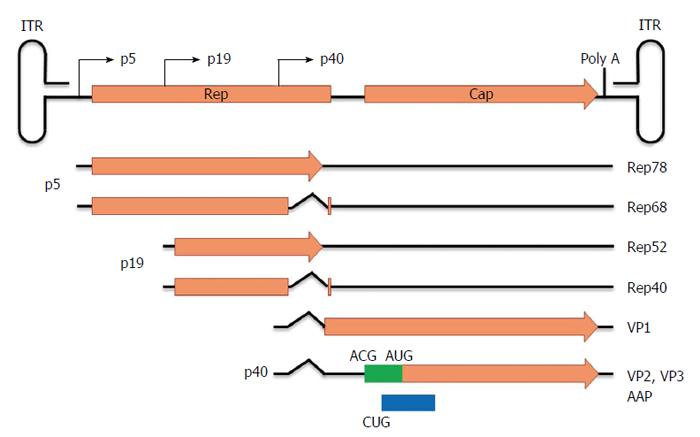
\includegraphics[width=10cm]{genoom.jpg}
	\caption{AAV genoomi skeem}
	\allikas{\cite{aav_genoom}}
	\label{aavgenoom}
\end{figure}
 
Viiruse genoom koosneb kolmest avatud lugemisraamist, mis kodeerivad kaheksat kolmelt promootorilt ekspresseeritud valku (Joonis \ref{aavgenoom}). Rep lugemisraam kodeerib nelja valku: Rep78 ja Rep68, mille valmistamiseks vajaliku mRNA süntees on alguse saanud p5 promootorilt, ning Rep52 ja Rep40, mille mRNA süntees on alguse saanud p19 promootorilt. Rep78 ja Rep68 on saadud samast pre-mRNA-st nii, et Rep68 jaoks on pre-mRNA splaissitud ja Rep78 jaoks tervikuks jäetud. Sama kehtib ka Rep52 ja Rep40 puhul. Kahel suuremal replikatsioonivalgul (Rep78 ja Rep68) esineb kohaspetsiifilise üheahelalise endonukleaasi, DNA helikaasi ja ATPaasi aktiivsus, mis on vajalik AAV DNA replikatsiooniks. Kaks väiksemat Rep-valku (Rep52 ja Rep40), mis on vajalikud AAV DNA pakkimiseks kapsiididesse, sisaldavad ainult ka suuremates valkudes esinevat helikaasi domeeni. \parencite{samulski}

Cap lugemisraam kodeerib nelja valku VP1, VP2, VP3 ja AAP. Kõikide nende valkude tootmiseks vajaliku ühise pre-mRNA tootmine on alguse saanud p40 promootorilt. Ühisest pre-mRNA-st on erinevaid valke kodeerivad mRNAd saadud pre-mRNA alternatiivse splaissimise teel. Nii moodustunud VP1, VP2 ja VP3 ühine osa on vajalik viiruse ikosaeedrilise kapsiidi moodustamiseks. Ainult VP1-s sisaldub oluline ensüüm fosfolipaas A2 ning VP1 ja VP2 ühisosas sisalduvad tuumalokatsiooniks vajalikud järjestused. AAP hõlbustab peamise kapsiidivalgu VP3 rakutuuma sisenemist ning soodustab kapsiidi kokkupanemist ja valmimist, kuid küpses kapsiidis AAP-d ei esine. \parencite{samulski}; \parencite{nature_aav}
 
\begin{figure}[htbp]
	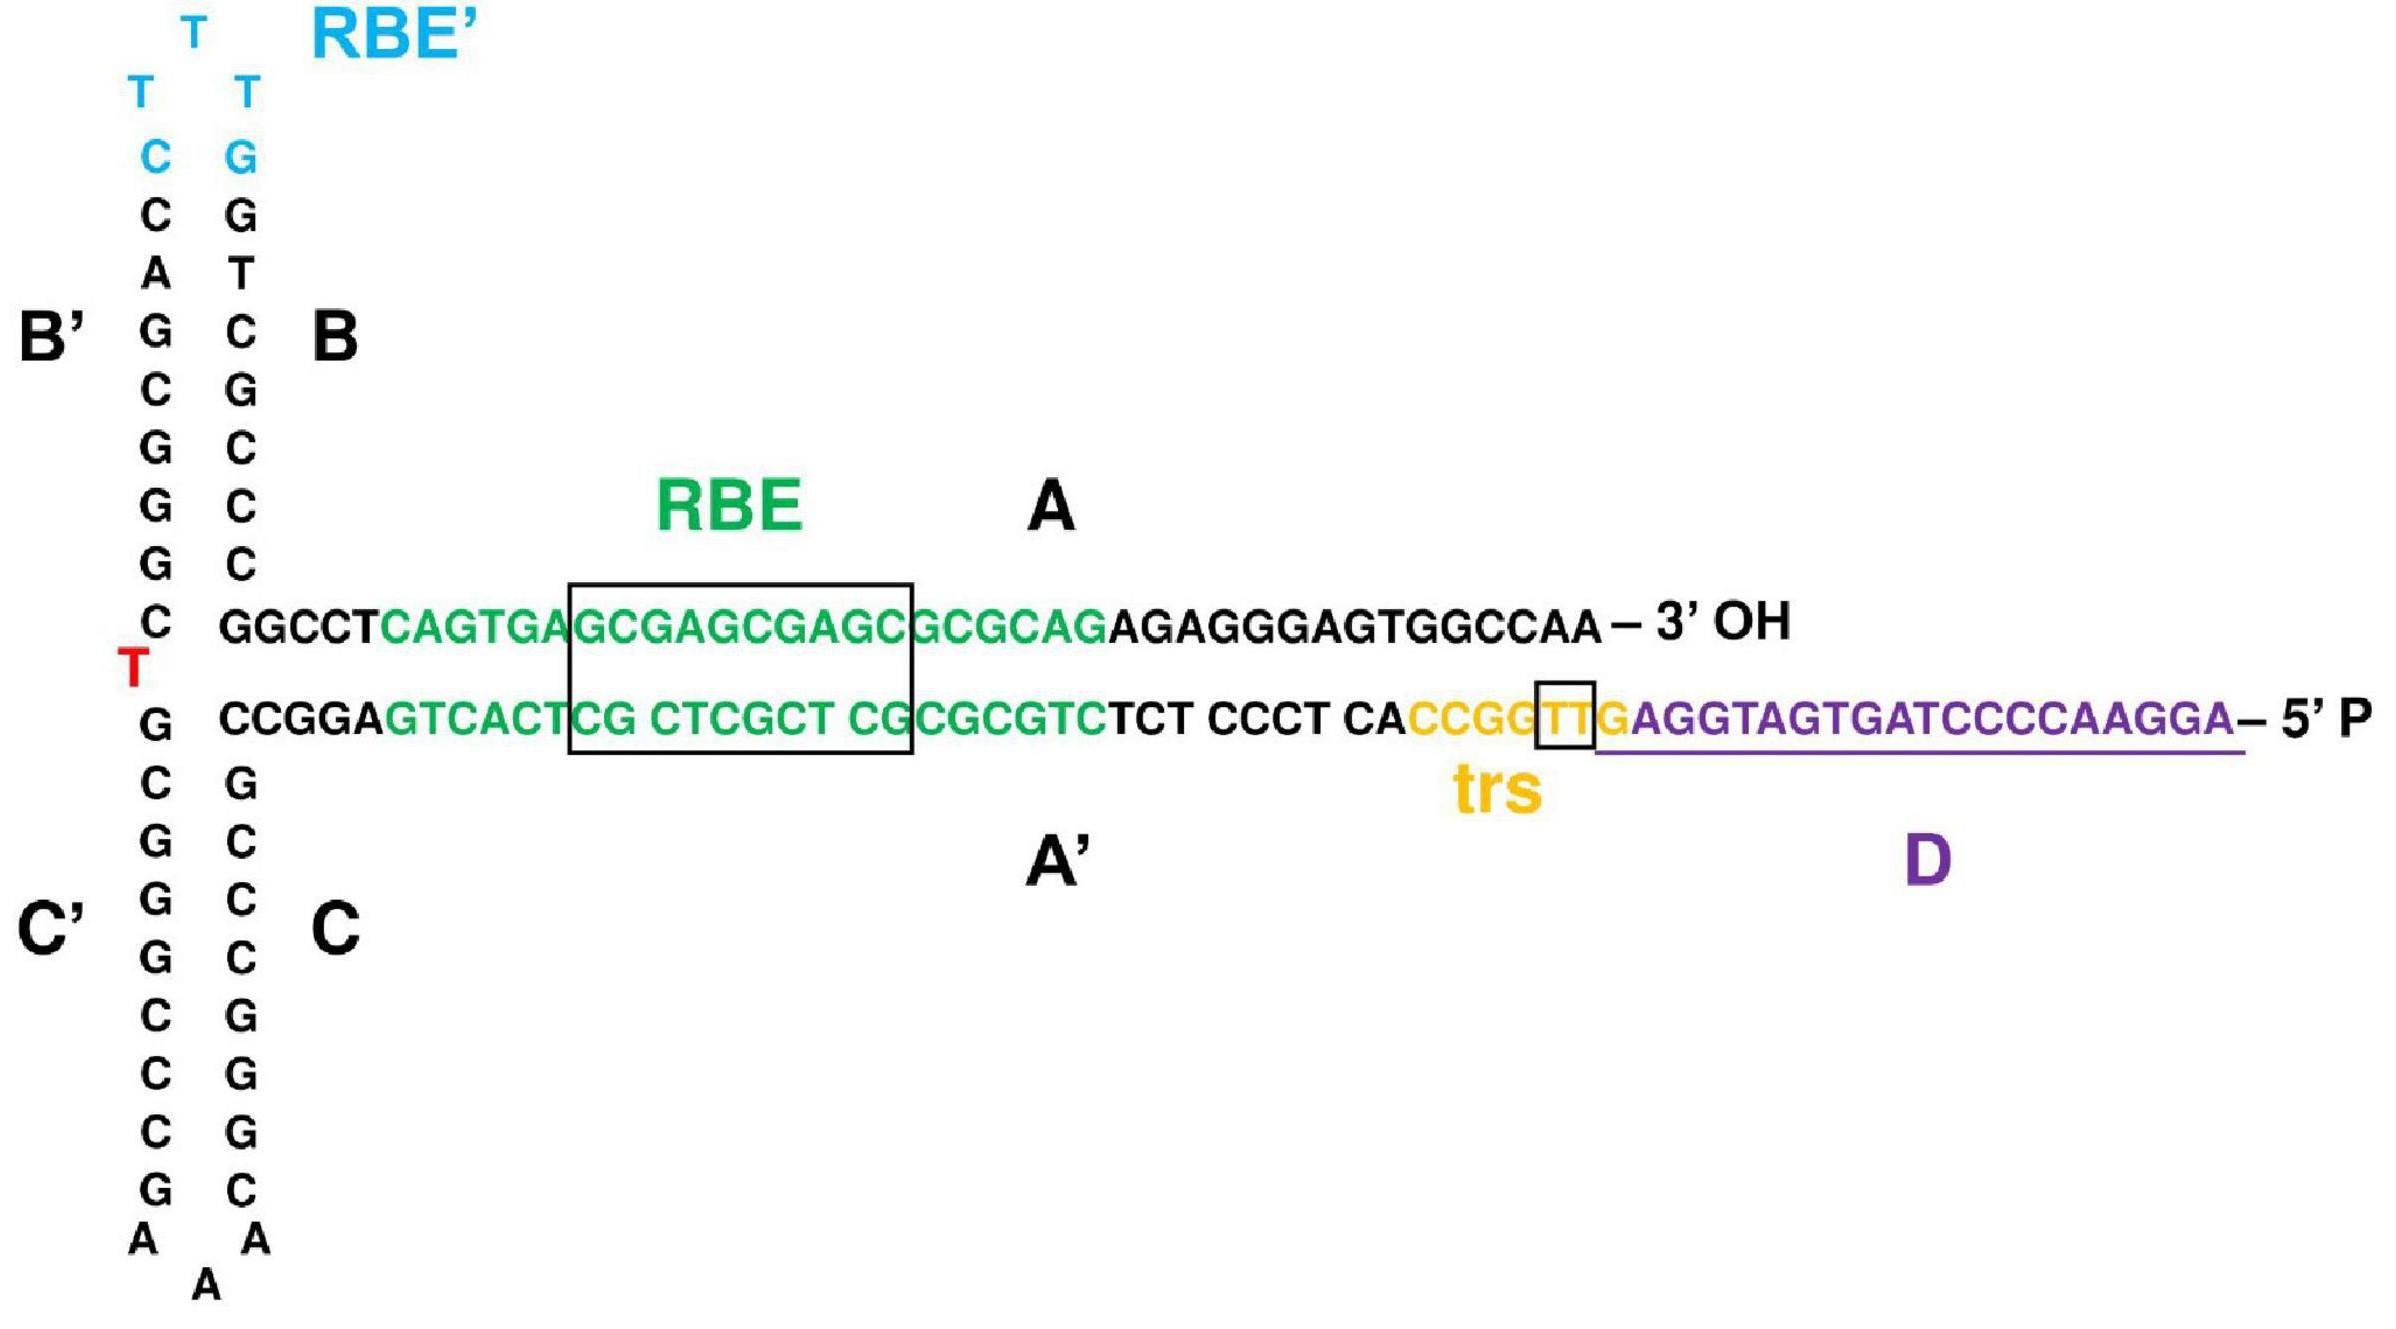
\includegraphics[width=10cm]{itr.jpg}
	\caption{AAV otsmine pöördkordusjärjestus}
	\allikas{\cite{itrmod}}
	\label{itr}
\end{figure}
 
AAV genoomi otstes asuvad 145 nukleotiidi pikkused otsmised pöördkordusjärjestused ehk ITR-id (Joonis \ref{itr}). ITR-idest algab AAV DNA replikatsioon, samuti on neil ka esmane DNA pakkesignaali funktsioon. Lisaks on ITR-id vajalikud AAV pärilikkusaine integreerumiseks peremeesraku genoomi \parencite{itrmod}. ITR-id on ka ainsad rekombinantsete AAV vektorite tootmiseks vajalikud \textit{cis}-toimelised järjestused ehk valke mitte kodeerivad DNA järjestused, mis on siiski olulised lähedal asuvate geenide transkriptsiooni reguleerimiseks. Kuigi AAV ITR-id võimendavad Rep-valgu juuresolekul transkriptsiooni, on Rep-valgu puudumisel minimaalne geeniekspressiooni reguleeriv roll. Seega peavad AAV vektorisse sisestatud transgeenid olema konstrueeritud sobiva geeniekspressiooni võimendavate transkriptsioonifaktorite, seostumissaitide, promootori, polü(A) ja splaissimissignaalidega, et tagada õige geeniekspressioon. \parencite{samulski}
 
\subsection{Viiruse kapsiid}

Adenoassptsieeritud viirusel on väike, kõigest \SI{25}{\nano\metre} diaameetriga ikosaeedriline kapsiid (Joonis \ref{aavkapsiid}), mis koosneb 60 molekulist. \parencite{samulski}. Võrdluseks võib öelda, et tavaliselt on viiruste läbimõõduks $\sim$\SI{100}{\nano\metre}. Ikosaeedrilisel kapsiidil on 20 kolmnurkset külge, AAV puhul koosneb iga kolmnurk kolmest alaosast. \parencite{viirusüld} Selline kapsiidiehitus muudab viirusosakese väga stabiilseks: see suudab taluda nii lühiajalist kuumust, happelist keskkonda kui ka kokkupuudet proteaasidega. Ikosaeedrilise AAV-osakese viiekiirelise sümmeetriatelje tipus on \SI{8,5}{\angstrom} läbimõõduga poor, mis arvatakse olevat viiruse DNA sisenemise kohaks. \parencite{samulski}

\begin{figure}[htbp]
	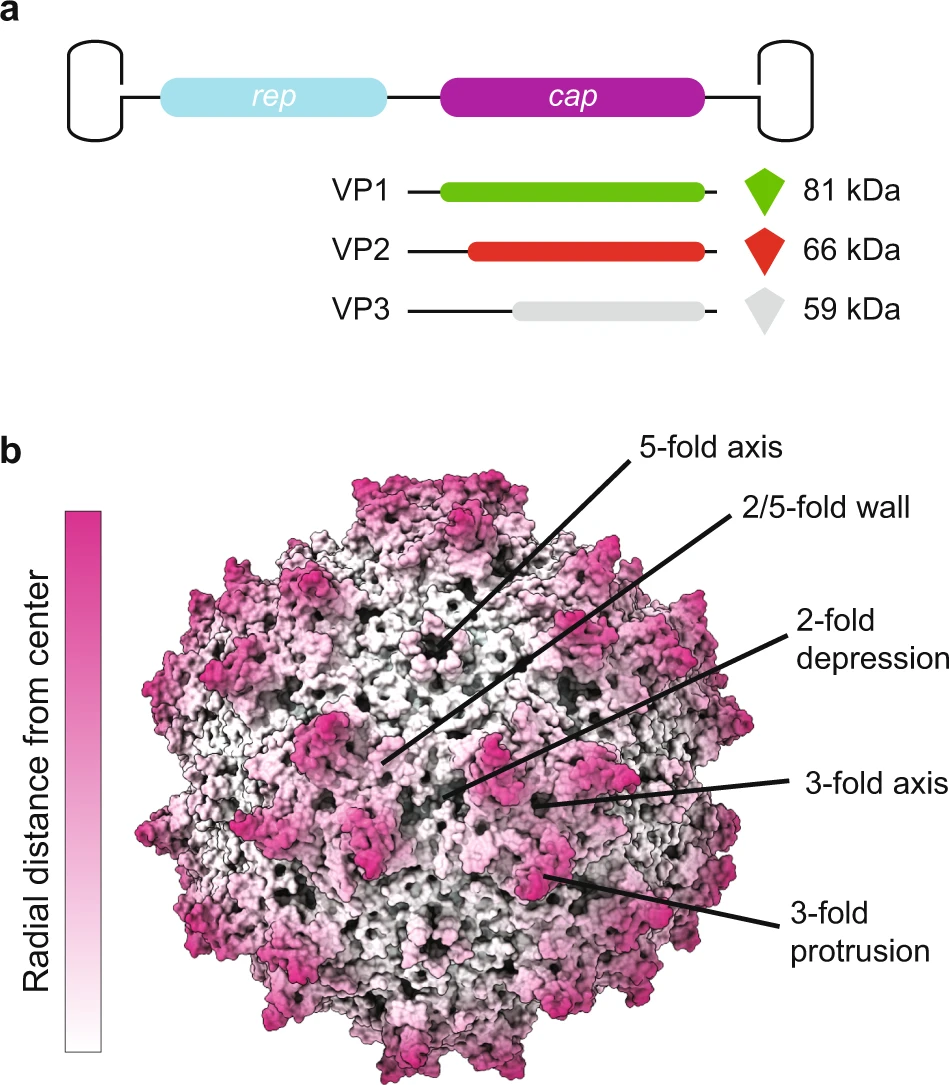
\includegraphics[width=7cm]{kapsiid.png}
	\caption{AAV kapsiidi ehitus}
	\allikas{\cite{nature_aav}}
	\label{aavkapsiid}
\end{figure}

Viiruse kapsiid koosneb kolmest erinevast viirusvalgust (VP), mis erinevad vaid oma N-otsade poolest. Kapsiid koosneb viirusvalkudest VP1, VP2 ja VP3 hinnanguliselt proportsioonis 1:1:10. Kapsiidi moodustamiseks ei ole ilmtingimata VP1 ja VP2 vaja, vaid terapeutilise geeni kohaleviimiseks vajaliku vektori moodustamiseks piisab ka ainuüksi VP3. Siiski tõstab VP1 ja VP2 olemasolu kapsiidi koostises toodetud viirusvektorite hulka ja nende transduktsiooni efektiivsust. Seda seetõttu, et VP1-l ja VP2-l on märgatav roll viiruse endotsütoosi teel rakku sisenemisel, viriooni endosomaalsel vabanemisel vesiikulist, viirusosakese rakutuuma sisenemisel ja viiruse genoomi vabanemisel kapsiidist. \parencite{nature_aav} 

\subsection{Adenoassotsieeritud viiruse paljunemine}

AAV rakku sisenemiseks seondub ta esmalt raku pinnal primaarse retseptoriga, milleks on proteoglükaanides leiduvad suhkrud, nagu siaalhape, galaktoos või heparaansulfaat \parencite{samulski}. Viiruse laia tropismi ehk võimet nakatada paljude eri kudede rakke selgitabki seondumine peaaegu kõikides rakudes toodetavate proteoglükaanidega \parencite{proteoglükaanid}. Rakku sisenemiseks peab viirus seostuma sekundaarse retseptoriga. Üheks tähtsaimaks selliseks retseptoriks on AAVR, mida on varasemalt tuntud ka KIAA0319L nime all ning mis on enamuse AAV serotüüpide rakku sisenemiseks hädavajalik. Täpsed sekundaarsed retseptorid, mida viirus rakku sisenemiseks kasutab erinevad serotüübiti, kuid mõned levinumad on FGFR1, CD9, $\alpha$V$\beta$5 integriin, $\alpha$5$\beta$1 integriin, HGFR, PDGFR, EGFR ja LamR. \parencite{pupo} Ühinenud rakupinnal olevate retseptoritega, siseneb viirus endotsütoosi teel klatriiniga kaetud vesiikulis rakku \parencite{samulski}. Klatriin on kuuest polüpeptiidahelast koosnev valk, mis hõlbustab vesiikuli eraldumist rakumembraanist \parencite{klatriin}.

Peale rakku sisenemist võib viirusosakesi leida peaagu kõigist tsütoplasmat sisaldavatest raku osadest. Esimese 2 tunni jooksul pärast nakatumist koguneb suurem osa viirusest tuumalähedasse tsütoplasmasse ja teeb sealses happelise pH-ga piirkonnas, mis on AAV infektsiooniks hädavajalik, läbi struktuurimuutuse. Seejärel siseneb AAV peremeesraku tuuma ning vabastab oma DNA seda kaitsnud kapsiidist. Kapsiidist vabanenud üheahelalise DNA põhjal sünteesitakse sellele komplementaarne DNA ahel. Nii moodustub kaheahelaline DNA genoom, mis on võimeline transkriptsiooniks. \parencite{samulski}

\begin{figure}[htbp]
	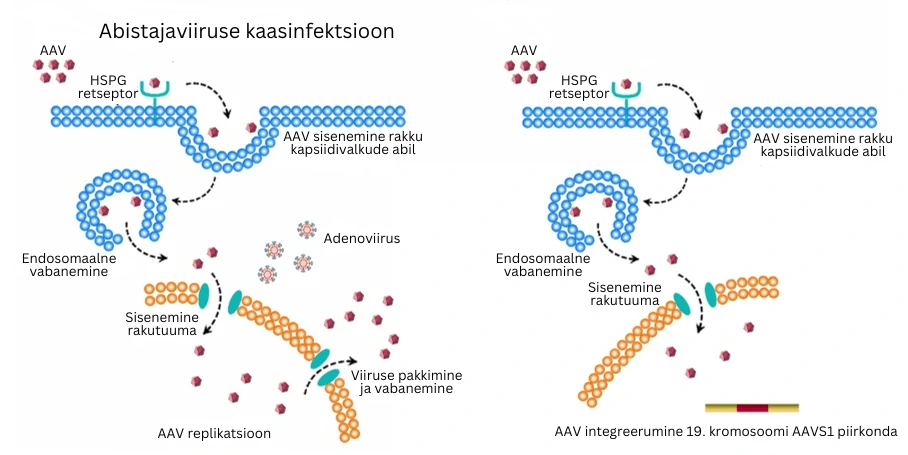
\includegraphics[width=14cm]{elu.png}
	\caption{AAV lüütiline ja lüsogeene tsükkel}
	\allikas{\cite{aav_elu}}
	\label{aavelu}
\end{figure}

Jõudnud peremeesraku tuuma võib AAV elutsükkel jätkuda, kas lüütiliselt või lüsogeenselt (Joonis \ref{aavelu}). Elutsükkel jätkub lüütiliselt, kui rakus esineb kaasinfektsioon abistajaviirusega, milleks on kas adenoviirus või herpesviirus. Viirus lülitub lüsogeensesse tsüklisse abistajaviiruse puudumisel, sel juhul represseeritakse viiruse geeniekspressioon. Peiteajal integreerub viiruse genoom eelistatult inimese 19. kromosoomi pikema õla ligikaudu \SI{4}{\kilo\base} pikkusesse piirkonda AAVS1 (Adeno-associated virus integration site 1) ning kandub nii rakujagunemisel tütarrakkudesse edasi. AAVS1 asub geeni MBS85 5' otsapoolses osas ning see paikneb lihasspetsiifiliste geenide TNNT1 ja TNNI3 lähedal. MBS85 on tuntud ka kui PPP1R12C ning see geen kodeerib müosiinfosfataasi alaühikut, mis reguleerib valgu fosfataas 1 delta katalüütilist aktiivsust ja aktiini tsütoskeleti kokkupanekut \parencite{PPP1R12C}. Kohaspetsiifilises integratsioonis mängivad olulist rolli AAV otsmine pöördkordusjärjestus (ITR), replikatsioonivalgud Rep78 ja Rep68 ning 138 aluspaari pikkune järjestus, mida nimetatakse integratsiooni efektiivsuse elemendiks (IEE). \parencite{elutsükkel}

Inaktiivses olekus AAV-d sisaldava raku nakatumisel abistajaviirusega lülitub viirus lüütilisse tsüklisse, mille käigus pääseb AAV proviiruse DNA peremeesraku kromosoomist ning aktiveeritakse AAV geeniekspressioon. Seejärel viiruse genoom replitseerub, toodetakse kapsiidivalke ning seejärel pakitakse need terviklikuks viriooniks. Rakust väljumiseks lüüsib abistajaviirus rakud, mille tulemusel vabanevad ka valminud AAV virioonid. Adenoviiruse geenide hulka, mis on abiks AAV geeniekspressioonil, kuuluvad E1a, E1b, E2a, E4 ja VA RNA. Herpesviirus aitab AAV geeni ekspressioonile kaasa, tuues rakku viiruse DNA polümeraasi ja helikaasi. AAV võib ka ilma abistajaviiruseta oma elutsükli lüütilisse faasi siseneda, kuigi sel juhul on efektiivsus madalam. Abistajaviiruseta pääseb AAV proviiruse DNA peremeesraku kromosoomist, kui peremeesrakku mõjutavad ainevahetuse inhibiitorid ehk raku ainevahetust aeglustavad ained või genotoksilised ühendid. \parencite{elutsükkel}
 
\subsection{Viiruse serotüübid}

Viiruse serotüübid erinevad teineteisest ainult kapsiidi valgulise ehituse poolest, genoom, välja arvatud kapsiidi määrav DNA järjestus, on neil kõigil sama. Loodusest leitud AAV serotüüpidest on enim uuritud serotüüpe AAV1-AAV13. Seetõttu öeldakse, et AAV-l on 13 looduslikku serotüüpi. Tegelikkuses leidub aga looduses sadu erinevaid AAV kapsiidi variante. Sõltuvalt kapsiidivalkudest omavad AAV serotüübid erinevate kudede osas erinevat tropismi ehk võimet nakatada eelistatult teatud koe rakke. \parencite{pupo} Järgnevalt kirjeldatud AAV-de kapsiidivalkude aminohappelised järjestused ning nende erinevused on  toodud lisas \ref{lisa-jarjestused}.

AAV1 serotüübi täpset päritolu pole teada, aga ilmselt pärineb see primaatidelt. Tema peamiseks retseptoriks on N-atsetüülitud siaalhape ning koretseptoriteks AAVR, GPR108, TM9SF2. Need retseptorid tekitavad AAV1 koespetsiifilist tropismi vööt-, sile- ja südamelihaskoe, kesknärvisüsteemi, kopsu, silma võrkkesta, kõhunäärme ja maksa rakkude suhtes. AAV1 on võrreldes teiste AAV looduslike serotüüpidega kõige efektiivsem vöötlihaskoe transdutseerimiseks. \parencite{pupo}; \parencite{serotüübid}

AAV2 pärineb inimpopulatsioonist ning seda peetakse kõige põhjalikumalt uuritud AAV serotüübiks. Sõltuvalt vanusest ja päritolust on hinnanguliselt 50\%-96\% meist AAV2 suhtes seropositiivsed. Tema peamiseks retseptoriks on heparaansulfaadi proteoglükaan. Sekundaarseteks retseptoriteks on AAVR, GPR108, TM9SF2, LamR, $\alpha$V$\beta$5 integriin, $\alpha$5$\beta$1 integriin, FGFR1, CD9 ja HGFR. AAV2 omab tugevamat tropismi vöötlihaskoe, kesknärvisüsteemi, maksa, neeru, võrkkesta, kopsu ja liigeste rakkude suhtes. \parencite{pupo}; \parencite{serotüübid}

AAV3 pärineb samuti inimpopulatsioonist. Sarnaselt AAV2-le on tema peamiseks retseptoriks HSPG. Teisesteks retseptoriteks on AAV3 puhul AAVR, GPR108, LamR, FGFR1 c-MET ja HGFR. Kuna esialgsetes uuringutes oli AAV3 transduktsiooni efektiivsus madal, jäeti see algselt geeniteraapiaks sobilike viirusvektorite kanditaadide hulgast välja. Hiljem avastati aga, et AAV3 omab tugevat tropismi inimese maksa kasvaja rakkude suhtes. Lisaks nakatab AAV3 ka eelkõige vöötlihaskoe, kesknärvisüsteemi ja sisekõrvas paiknevaid kuulmerakke. \parencite{pupo}; \parencite{serotüübid}

AAV4 kapsiidivalkude järjestused erinevad keskmiselt suuremal määral teiste AAV-de kapsiidivalkude järjestustest, sarnanedes AAV2-le kõigest 58\% ulatuses. AAV4 pärineb primaatidelt, arvatavasti Aafrika roheahvidelt. AAV4 kapsiidi pinna struktuur sarnaneb üllataval kombel naaritsate aleuudi haiguse viiruse (ADV) ja inimese parvoviiruse B19-ga, mis kuuluvad AAV-ga samasse perekonda. AAV 4 peamiseks retseptoriks on O-atsetüülitud siaalhape ning teiseseks retseptoriks GPR108. AAV4 omab tugevamat tropismi kesknärvisüsteemi, silma võrkesta, kopsu, neeru ja südamelihaskoe rakkude suhtes. \parencite{aav4}; \parencite{pupo}; \parencite{serotüübid}

AAV5 on teistest looduslikest AAV kapsiidivariantidest kõige erinevam. Võrreldes AAV2 ja AAV8-ga on tema kapsiid ainult 57\% ulatuses homoloogiline ning AAV10-ga on kapsiidihomoloogia samuti vaid 58\%. Võrdluseks on teistel AAV serotüüpidel omavaheline homoloogia märksa suurem, ligikaudu 80\%. AAV5 pärineb inimestelt ning see on ühtlasi ka ainus AAV serotüüp, mis on otse inimese kudedest eraldatud. Selle peamiseks retseptoriks on N-atsetüülitud siaalhape ning koretseptoriteks AAVR, PDGFR ja TM9SF2. AAV5 nakatab eelkõige vöötlihaskude, kesknärvisüsteemi, kopse, silma võrkkesta ja maksa. \parencite{pupo}; \parencite{serotüübid}

AAV6 on homoloogiliselt väga sarnane AAV serotüüpidega 1 ja 2, olles eri piirkondades, kas AAV1 või AAV2-ga peaaegu identne. Seetõttu arvatakse, et AAV6 on tekkinud nende kahe homoloogilise rekombinatsiooni käigus \parencite{aav6}. See AAV serotüüp on pärit inimeselt ning selle peamisteks retseptoriteks on HSPG ja N-atsetüülitud siaalhape. Teisesteks retseptoriteks on AAV6-l AAVR, GPR108, TM9SF2 ja EGFR. AAV6 omab kõrgemat tropismi vöötlihaskoe, südamelihaskoe, maksa, kesknärvisüsteemi, silma võrkkesta, kopsu ja teiste hingamiselundkonna rakkude suhtes. \parencite{pupo}; \parencite{serotüübid}

AAV7 avastati reesusmakaakidelt. Selle serotüübi rakule kinnitumise ja rakku sisenemise metoodika pole täpselt teada, küll aga teatakse, et AAV7 ei kasuta rakule kinnitumiseks HSPG-d \parencite{glykaanid}. Teisesteks retseptoriteks on AAV7-l GPR108 ja TM9SF2. AAV7 nakatab eeskätt vöötlihaskoe, kesknärvisüsteemi, silma võrkkesta ja maksa rakke. \parencite{pupo}; \parencite{serotüübid}

AAV8 leiti samuti reesusmakaakidelt ning nagu AAV7-l ei ole teada selle primaarset retseptorit. AAV8 sekundaarseteks retseptoriteks on AAVR, GPR108, TM9SF2 ja LamR. AAV8 nakatab maksa, vöötlihaskoe, kesknärvisüsteemi, võrkkesta, kõhunäärme, südamelihaskoe, neerude ja rasvkoe rakke. AAV8 91\% ulatuses sarnanev AAVrh.8 suudab erinevalt teistest eelpool mainitud AAV serotüüpidest ületada vere-aju barjääri \parencite{AAVrh.8}. AAVrh.8 leitud sekundaarseks retseptoriks on GPR108 ning see omab kõrgemat tropismi vöötlihaskoe, maksa ja kesknärvisüsteemi rakkude suhtes. \parencite{pupo}; \parencite{serotüübid}

AAV9 leiti inimeselt ning suudab samuti ületada vere-aju barjääri. Lisaks neuronite suudab AAV9 ajus nakatada ka neuronite tööks hädavajalikke astrotsüüte \parencite{bbb}. AAV9 primaarseks retseptoriks on N-atsetüülgaloktosamiin. Sekundaarseteks retseptoriteks on AAV9 puhul AAVR, GPR108, TM9SF2 ja LamR. Antud serotüüp nakatab eelistatult maksa, kopsu, kõhunäärme, kesknärvisüsteemi, võrkkesta, neerude, munandite, südame- ja vöötlihaskoe rakke. \parencite{pupo}; \parencite{serotüübid}

AAV10 avastati jaava makaakidelt ning selle rakule kinnitumiseks ja sellesse sisenemiseks vajalikke retseptorid on teadmata. AAV10 on leitud kõrgem tropism südamelihaskoe, kopsu, maksa, neeru ja emaka rakkude suhtes. AAVrh.10 pärineb reesusmakaakidelt ning suudab sarnaselt AAV9-le ületada vere-aju barjääri ja nakatada astrotsüüte \parencite{bbb}. Selle serotüübi teisesteks retseptoriteks on GPR108 ja LamR. AAVrh.10 nakatab eeskätt maksa, neeru, kopsu, kõhunäärme, kesknärvisüsteemi, võrkkesta, vööt- ja südamelihaskoe rakke. \parencite{pupo}; \parencite{serotüübid}

AAV11 pärineb jaava makaakidelt ning selle retseptorid pole teada. AAV11 nakatab eelistatult neeru, põrna, kopsu, mao, vööt- ja südamelihaskoe rakke. AAV12 ja AAV13 pärinevad mõlemad primaatidelt ning nende rakku sisenemise mehhanismid on teadmata. AAV12 omab kõrgemat tropismi vöötlihaskoe ja süljenäärmete suhtes. AAV13 on hetkel veel vähe uuritud, kuid on teada, et see sarnaneb enim AAV2 ja AAV3-ga. \parencite{pupo}; \parencite{serotüübid}

\subsection{AAV kasutamine geeniteraapias}

Adenoassotsieeritud viirused avastati saasteainena 1965. aastal ahvi adenoviiruse preparaadist \parencite{aav-avastamine}. Mõni aasta hiljem eraldati seda juba inimkudedest \parencite{aav-gen}. Nüüdseks on rekombinantse AAV kaasutamine saanud üheks perspektiivikaimaks geeniteraapia rakendamise viisiks ning see on kõige laialdasemalt kasutatav viirusvektor \parencite{aavlevinuim}. Esimene AAV-l põhinev ravi Glybera, mis ravib lipoproteiini lipaasi vaegust, sai Euroopas heakskiidu 2012. aastal. Hetkel on kliinilise uuringu faasis üle saja AAV-l põhineva geeniteraapia protokolli \parencite{who}. 2023. aasta seisuga on Euroopa Liidus lisaks Glyberale müügiloa saanud viis AAV põhist geeniravi: Luxturna, Zolgenmsa, Upstaza, Roctavian ning Hemgenix. Need ravivad vastavalt RPE65 puudulikkusest põhjustatud retinaalset düstroofiat ja spinaalset lihasatroofiat, aromaatse L-aminohappe dekarboksülaasi (AADC) puudulikkust ning A- ja B-hemofiiliat \parencite{ravimiamet}. 

Geeniteraapia valdkonnas AAV uurimiseks ning käsitlemiseks kui perspektiivika viirusvektorina on mitmeid põhjuseid. Üks põhjustest on AAV võrdlemisi madal immunogeensus ehk immuunvastuse esilekutsumise tõenäosus \parencite{pupo}. Samuti ei põhjusta AAV inimestes teadaolevalt mitteühtegi haigust, mis muudab nendega töötamise tunduvalt ohutumaks. Bioohutust tõstab veelgi viiruse enda geneetilise materjali eemaldamine viirusvektorist. \parencite{aav-gen} AAV laia kasutamise põhjuseks on ka viiruse lai tropism, mis võimaldab AAV vektoritega transdutseerida peaaegu, et kõiki kudesid \parencite{laitropism}.

Kuna paljudel inimestel esineb juba AAV looduslike serotüüpide vastane immuunsus, tuleb AAV efektiivseks kasutamiseks leida viis sellest mööda pääsemiseks. Samuti peab vältima uute humoraalsete ja rakuliste imuunvastuste tekkimist \parencite{pupo}. Piiranguid AAV laialdasele kasutamisele seab ka selle genoomi väike suurus, mis takistab suurte transgeenide pakkimist. Selle probleemi ületamiseks on proovitud sisestatav transgeen mitme AAV vahel ära jaotada. Sellisel meetodil pakitud transgeeni ekspressioon pole aga osutunud nii tõhusaks kui ühtsena pakitud transgeeni oma. \parencite{geenilõhkumine}

\subsection{AAV kapsiidide modifitseerimine peptiididega}

Kuigi geeniteraapia katsed nii-öelda metsiktüüpi AAV-dega ehk looduslike AAV serotüüpidega on andnud edukaid tulemusi, on kliinilistes katsetes selgunud, et metsiktüüpi AAV serotüübid geeniteraapia ravimites ei ole tihti efektiivsed, sest sageli on täiskasvanud patsientidel nende vastu juba väljakujunenud immuunsus. Näiteks hiljuti heakskiidetud geeniteraapia ravim Elevidys Duchenne’i lihasdüstroofia ravimiseks põhineb reesusmakaagi AAV serotüübil rh74, kuid isegi selle haruldase serotüübi puhul peetakse vajalikuks teha suunatud mutatsioone. \parencite{elevidys}
%ka täiesti selgeks saanud, et loodusliku kapsiidiga AAV vektorid ei ole võimelised saavutama AAV täit potentsiaali. Seda seetõttu, et AAV ei ole arenenud eesmärgiga nakatada spetsiifilisi rakke ja toimetada kohale teraupeutilise toimega geene. \parencite{modifitseerimine}
Seetõttu pööratakse viimasel ajal rohkem tähelepanu rekombinantsete AAV viirusvektorite arendamisele. Looduslikult AAV serotüübile vastava tropismi muutmiseks või selle võimendamiseks saab luua kimäärseid AAV-sid, mille kapsiid koosneb mitme erineva serotüübi järjestusest. Neid on võimalik luua sisestades peptiide või isegi terveid valke kodeerivaid DNA-järjestusi kindlatesse viiruse kapsiidigeeni piirkondadesse \parencite{pupo}. 

\begin{figure}[htbp]
	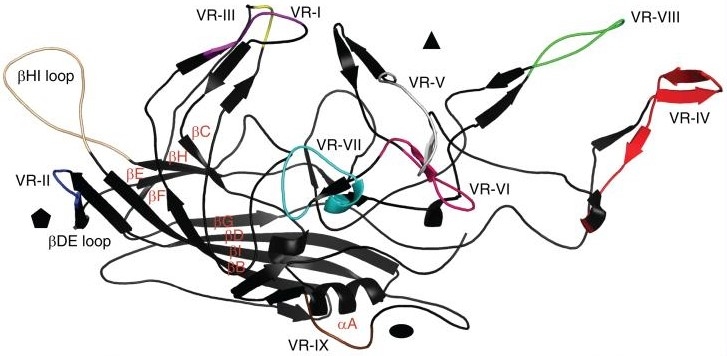
\includegraphics[width=10cm]{vr11.jpg}
	\caption{VP3 monomeer üheksa VR-iga}
	\allikas{\cite{vrjoonis}}
	\label{vrjon}
\end{figure}

AAV kapsiidi pinnal VP3-s leiduvates $\beta$-ahelate ühenduskohtades ehk pinnasilmustes esinevad struktuuriliselt varieeruvad piirkonnad (VR-id) (Joonis \ref{vrjon}). Need pinnasilmused kleepuvad kokku, tekitades kapsiidi pinnal variatsioone. Eeldatakse, et erinevustest VR-ide kokkuhaakumises, sõltub rakuline tropism ja koetransduktsiooni efektiivsus. \parencite{vr-basic} AAV kapsiidi pinnal saab eristada üheksat muutuvat piirkonda \parencite{vrjoonis}. VR-IV, VR-V ja VR-VIII moodustavad eendite ülaosas silmuseid, samas kui VR-VI ja VR-VII asuvad eendite alaosas. Nende VR-ide avatud, mitte kapsiidi struktuuri moodustamiseks asendi, ja retseptoriga seondumise funktsiooni tõttu, on VR-id ideaalsed kapsiidi modifitseerimiseks ja neisse peptiidide sisestamiseks. \parencite{modifitseerimine}

\section{Golden Gate kloneerimine}

Molekulaarne kloneerimine on protsess, mille käigus kombineeritakse kokku mitu DNA fragmenti üheks plasmiidiks, mida saab seejärel paljundada bakterites (tavaliselt \textit{Escherichia coli}'s). Kõige tavalisem praktika selle protsessi läbiviimiseks on esmalt olemasolevaid DNA-sid restrikteerida ehk lõigata neist välja vajaminevad DNA-fragmendid. Seejärel eraldatakse saadud DNA-fragmendid üksteisest geelelektroforeesi teel, millele järgneb nende väljapuhastamine geelist. Viimaseks etapiks on selle protsessi puhul saadud fragmentide kokku ligeerimine. Selline viis rekombinantse DNA saamiseks on aga töö- ja ajamahukas protsess, mis hõlmab enda mitmeid etappe, mis võivad ebaõnnestuda. \parencite{ggkloneerimine}

\begin{figure}[htbp]
	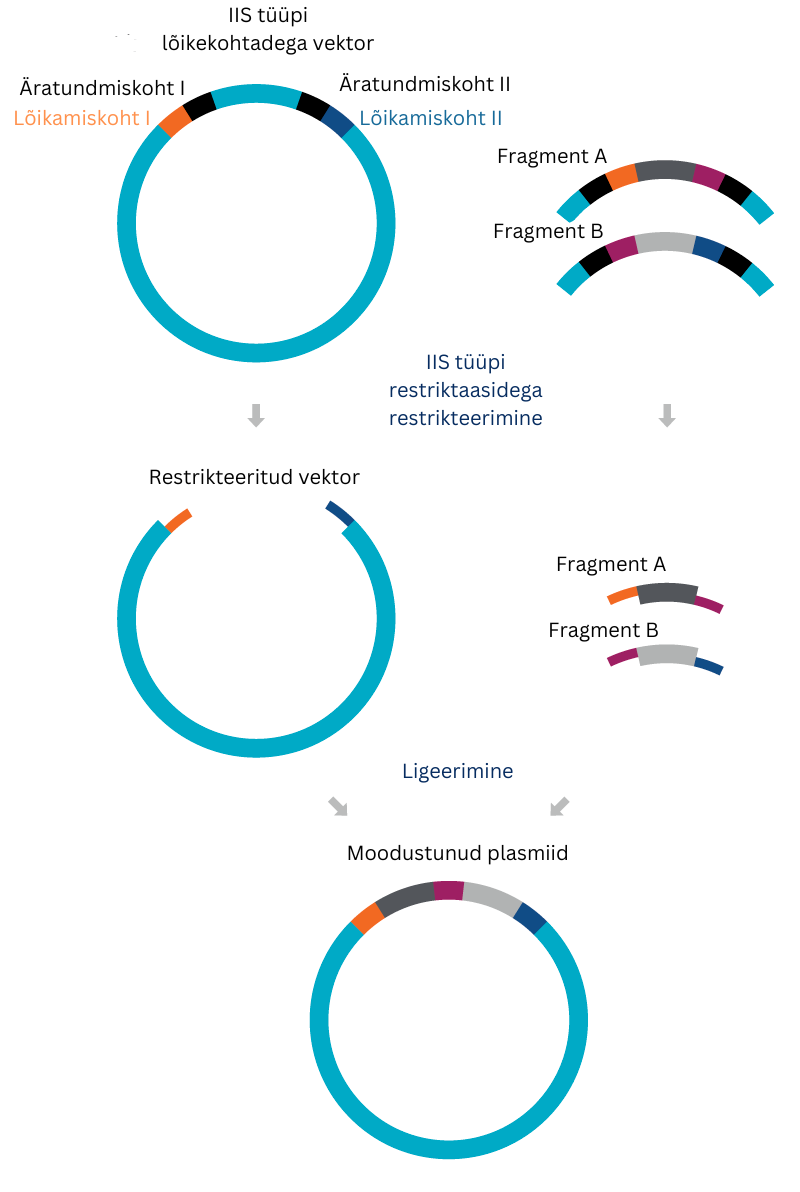
\includegraphics[width=8cm]{gg.png}
	\caption{Golden Gate kloneerimine}
	\allikas{\cite{ggjoonis}}
	\label{ggjoonis}
\end{figure}

Mõnevõrra lihtsam molekulaarse kloneerimise meetod on Golden Gate kloneerimine. Golden Gate kloneerimise meetod erineb tavapärasest DNA rekombineerimisest selle poolest, et see võimaldab korraga ühes reaktsioonisegus teostada nii restrikteerimist kui ka ligeerimist, kusjuures fragmente pole vaja geelist puhastada (Joonis \ref{ggjoonis}). \parencite{ggkloneerimine} Sellise kloneerimisviisiga on korraga ühte plasmiidi viidud kuni 52 DNA-fragmenti \parencite{gg52}. Golden Gate metoodika eeldab aktseptorvektori ja doonorvektorite eelnevat konstrueerimist, millesse on sisse disainitud üks või mitu sobivate restriktaaside äratundmiskohta. Golden Gate kloneerimisel kasutatakse ainult teatud tüüpi IIS restriktaase, mis tekitavad 4 nukleotiidi suurusi 5‘ üleulatuvaid otsi (BbsI, BsaI, Esp3I ja SapI), mis võivad olla ükskõik, millise järjestusega. See võimaldabki Golden Gate metoodikat rakendada paljude insertide sisestamiseks ühte vektorisse kindlas järjekorras, kuna teoreetiliselt on võimalik disainida 256 erinevat üleulatuvat järjestust. \parencite{256}
%Hoolimata Golden Gate metoodika eelistest ei saa seda kasutada ilma sobiva aktseptorvektorita, millesse on sisse disainitud üks või mitu restriktaasi äratundmiskohta. Golden Gate kloneerimisel kasutatakse ainult teatud tüüpi IIS restriktaase (BbsI, BsaI, BsmBI, Esp3I ja SapI), mis seab piirangud Golden Gate metoodika rakendusvõimalustele, sest enamus plasmiididel ei ole nedele restriktaasidele vajalikke äratundmiskohti. \parencite{ggkloneerimine}

\begin{figure}[htbp]
	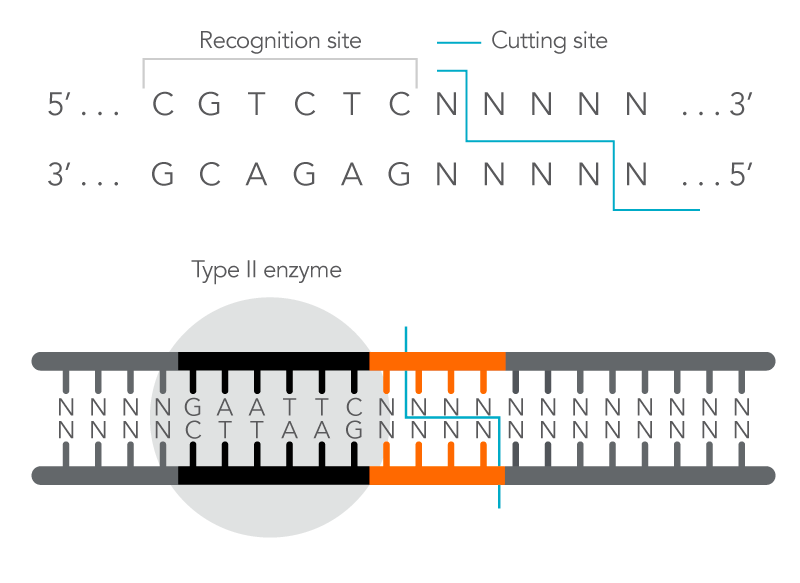
\includegraphics[width=7cm]{restriction-enzyme_s-recognition-site-differs-from-its-cutting-site.png}
	\caption{Restrikteerimine IIS tüüpi restriktaasiga}
	\allikas{\cite{ggjoonis}}
	\label{restriktaas}
\end{figure}

Täpsemalt töötab Golden Gate kloneerimine nii, et IIS tüüpi restriktaas lõikab DNA fragmente oma äratundmiskohast veidi eemal ning tekitab kas 3’ või 5’ üleulatuvaid otsi (Joonis \ref{restriktaas}) \parencite{restr}. Kuna restriktaasi äratundmis- ja lõikamiskoht ei ühti, siis võib üleulatuva otsa nukleotiidijärjestus olla ükskõik milline, seega, vastavalt vajadusele luuakse kindlate järjestustega fragmentide otsad \parencite{ggjoonis}. Seejärel ligeeritakse erinevate DNA fragmentide üleulatuvad otsad omavahel T4 DNA ligaasi abil kokku. Seda võimaldavad sama restriktaasi kasutamisel tekkinud ühepikkused üleulatuvad otsad ning plasmiidide konstueerimine selliselt, et vajaminevad DNA fragmendid ei sisaldaks ühtegi IIS restriktaasi äratundmiskohta. Lõpptulemusena moodustub ainult korrektne DNA plasmiid, nii-öelda üle jäänud DNA lõigud  kogunevad puhverlahusesse. \parencite{ggkloneerimine}; \parencite{ggkloneerimine_userguide}

\chapter{Eksperimentaalne osa}

\section{Töö eesmärk}

Käesoleva töö eesmärkideks on:\\
1) Golden Gate kloneerimiseks sobiliku platvormi loomine AAV kapsiidide modifitseerimiseks;\\
2) eeldatavalt kopsukoe ja vähkkasvaja spetsiifiliste peptiidide sisestamine AAV2 ja AAV8 kapsiididesse;\\
3) uute kapsiidivariantidega viiruste tootmine ja testimine. 

\section{Materjalid ja metoodika}

\subsection{Töös kasutatud plasmiidid}

Töös on kasutatud olemasolevaid AAV vektorite plasmiide: pHelper, pRC2 (Takara Bio), pAAV2/8 (Addgene, plasmiid nr 112864), lühendatud AAVcap2 ja lühendatud AAVcap8 ning AAV8 VR-IV ja VR-VIII vasakuid ja paremaid õlgu kodeerivad plasmiidid (IVEX Lab, Liisa Pata). Lisaks kasutati IVEX Lab OÜ-s disainitud ja ettevõttest Twist Biosciences tellitud sünteetilisi DNA plasmiide (Q1-Q8). Plasmiidid transformeeriti kompetentsetesse bakterirakkudesse (\textit{Escherichia coli} tüvi DH5$\alpha$) ning kasvanud kolooniatest eraldati aluselise lüüsi meetodil FavorGen FavorPrep Plasmid Extraction Mini Kiti ja tootja protokolli abil plasmiidse DNA minipreparatsioonid. Eraldatud DNA-st restrikteeriti 1-2 \si{\micro\gram} restriktaasidega EcoRI ja HindIII ning tekkinud fragmendid lahutati üksteisest elektroforeesiga 1,5\% TAE-agaroosgeelil. Õiged fragmendid lõigati geelist välja ning neist puhastati DNA kolonnidega FavorGen FavorPrep GEL/PCR Purification Kitiga vastavalt tootja protokollile. Plasmiidist Q1 eraldati peptiidi uCendR ning AAV2 kapsiidi VR-VIII paremat ja vasakut õlga kodeerivad DNA järjestused. Plasmiididest Q2 ja Q3 vastavalt peptiide LuS7A ja uEdbTnc kodeerivad DNA järjestused. Plasmiidist Q4 peptiidi abIntNRP ja AAV5 kapsiidi VR-IV parema ja vasaku õla kodeerivad DNA järjestused. Plasmiididest Q5-Q7 eraldati vastavalt peptiide LuVG, IVEX1 ja LinTT1 ning plasmiidist Q8 peptiidi XBB1.5 ja AAV2 kapsiidi VR-IV paremat ja vasakut õlga kodeerivad DNA järjestused.

\subsection{Töös kasutatud peptiidide ja oligonukleotiidpraimerite järjestused}

Töös kasutatud peptiidide aminohappelised- ja oligonukleotiidpraimerite nukleotiidjärjestused on toodud järgnevalt. 

Peptiidi IVEX1, mis on disainitud IVEX Lab OÜ-s, järjestus on HSRGDPRRSVST. SARS-CoV-2 tüve Omikron XBB1.5 ogavalgu RBD domeeni osa on töös valitud GVAGPANTSPLAYGFRP, mis põhineb NCBI valguandmebaasis avaldatud järjestusel \parencite{spike}. Peptiidi uCendR järjestus on RPARSGRSAGGSVA \parencite{ucendr}. LinTT1 järjestus on AKRGARSTA \parencite{lintt1}. LuS7A järjestus on APWHLSAQYSRT \parencite{lus7a}. LuVG järjestus on KDNTPGR \parencite{luvg}. Peptiidide uEdbTncC ja $\alpha$v$\beta$3-Int-NRP1 järjestused on vastavalt PPRRGLIALKTSSAGGSVA ja RGDSGSGATWLPPR, mis pärinevad Tambet Teesalu patendist EP3921329A1.

Golden Gate aktseptorplasmiidide konstrueerimiseks vajalikud praimerid:\\
GGA.Cap2-5 5'-TTG AAG CTT GAA GAC TGC TAG CTT CAT CAC ACA GTA CT-3';\\
GGA.Cap5-5 5'-TTG AAG CTT GAA GAC TCT CGA GGG CAA CAT GCT CA-3';\\
GGA.Cap5-3 5'-ATG AAG CTT GAA GAC GGG ATC CGC TGG GTC CA-3';\\
GGA.Cap8-3 5'-ATG AAG CTT GAA GAC ACG TAC GGC AGC TGG TAC TCC-3';\\
GGA.Cap8-5 5'-TTC AAG CTT GAA GAC AAC CGG TTG ATT CGT TTC AGT T-3';\\
GGA.Cap9-3 5'-ATG AAG CTT GAA GAC ACG TAC GGG AGC TGA TAG TC-3';\\
GGA.Cap9-5 5'-TTC AAG CTT GAA GAC CGG ATC CTC CAA CGG CCT-3'.

Valmis kapsiidi kodeerivate plasmiidide sekveneerimiseks vajalikud praimerid:\\
Cap5\_seqF1 5'-CCC TTC CAC TCC AGC TTC-3';\\
Cap2\_seqF1 5'-TCC TTT CCA CAG CAG CTA C-3';\\
Cap8\_seqF1 5'-TAC TTA CAC CTT CGA GGA CG-3';\\
Cap8\_seqF2 5'-CGA TGT CAT GCT CAC CAG-3';\\
Cap9\_seqF1 5'-CTA CGC TCA CAG CCA AAG-3'.

Sinivalget selektsiooni võimaldava kanamütsiini resistentse plasmiidi konstrueerimiseks vajalikud praimerid:\\
LacZ$\alpha$-3Ade 5'-GTG TCA CGT AGT GTC GGG GCT GGC TTA ACT A-3';\\
%LacZ$\alpha$-5Vsp 5'-ACT CAT TAA TCA CCC CAG GCT TTA CAC TTT ATG T-3';\\
pBR322oriF 5'-GGG AAA CGC CTG GTA TCT TT-3'.

\subsection{Ligeerimine ja transformeerimine}

Ligeerimissegu, mille kogumaht oleks \SI{10}{\micro\litre}, valmistamiseks segati kokku $\sim$\SI{5}{\micro\litre} vajaminevat DNA-d, \SI{0,6}{\micro\litre} T4 DNA ligaasi, \SI{1}{\micro\litre} 10X T4 DNA ligaasi puhvrit ning lahjendati destilleeritud veega \SI{10}{\micro\litre}. Seejärel jäeti ligeerimissegu tavaliselt üle öö toatemperatuurile ligeerima. 

Transformeerimiseks segati $\sim$\SI{10}{\micro\litre} ligeerimissegu kokku $\sim$\SI{70}{\micro\litre} \SI{-80}{\celsius} hoiustatud bakterirakkudega (\textit{Escherichia coli} tüvi DH5$\alpha$). Segu inkubeeriti jääl 45 minutit, millele järgnes kuumašokk \SI{42}{\celsius} 1 minut. Peale kuumašokki pandi transformatsioonisegu paariks minutiks tagasi jääle. Kui bakterisse viidi ampitsilliiniresistentsusega plasmiid, külvati segu seejärel otse Petri tassil olevasse LB-tardsöötmesse, mis sisaldas \SI{100}{\micro\gram\per\milli\litre} ampitsilliini. Kanamütsiiniresistentsusega plasmiidi puhul lisati transformatsioonisegule \SI{800}{\micro\litre} LB-vedelsöödet ning inkubeeriti saadud segu 45 minutit \SI{180}{\rpm} juures. Bakteriloksutist võetud segust kanti \SI{100}{\micro\litre} Petri tassil olevasse LB-tardsöötmesse, mis sisaldas \SI{50}{\micro\gram\per\milli\litre} kanamütsiini. Tasse inkubeeriti üle öö \SI{37}{\celsius} juures ning seejärel hoiustati \SI{4}{\celsius} juures. 

\subsection{Plasmiidse DNA eraldamine aluselise lüüsi meetodil}

Plasmiidse DNA eraldamiskes külvati Petri tassidel kasvanud bakterikolooniad katseklaasi, mis sisaldas \SI{4}{\milli\litre} LB-vedelsöödet ja vastavalt bakterisse viidud plasmiidi tekitavale antibiootikumiresistentsusele, kas \SI{100}{\micro\gram\per\milli\litre} ampitsilliini või \SI{50}{\micro\gram\per\milli\litre} kanamütsiini. Inokuleeritud katseklaase ehk katseklaase, kuhu oli viidud bakterid, inkubeeriti üle öö \SI{37}{\celsius} juures loksutil kiirusega \SI{180}{\rpm} (pööret minutis). 

Bakteritest plasmiidse DNA eraldamiseks aluselise lüüsi meetodil kasutati FavorGen FavorPrep Plasmid Extraction Mini Kiti ja tootja protokolli. \SI{2}{\milli\litre} eppendorfi valati katseklaasist bakterisegu ning tsentrifuugiti \SI{30}{\second} \SI{11000}{\g} juures, bakterirakud kogunesid eppendorfi põhja ning ülejäänud bakterisööde kallati ära, protsessi korrati veel ühe korra. Seejärel lisati bakteritele \SI{240}{\micro\litre} FAPD1 puhvrit ning suspendeeriti need selles vortexi abil täielikult. Lüüsimiseks lisati eppendorfidesse \SI{240}{\micro\litre} FAPD2 puhvrit, loksutati neid $\sim$10 korda ning inkubeeriti toatemperatuuril $\sim$4 minutit. Neutraliseerimiseks lisati lahustele \SI{360}{\micro\litre} FAPD3 puhvrit, loksutati neid $\sim$10 korda ning tsentrifuugiti 5 minutit \SI{16100}{\g} juures. Lüsaat kanti kogumistuubis olevasse kolonni ning tsentrifuugiti \SI{30}{\second} \SI{11000}{\g} juures. Läbivoolanud vedelikust vabaneti ning kolonni lisati \SI{400}{\micro\litre} WP puhvrit, tsentrifuugiti \SI{30}{\second} \SI{11000}{\g} juures, läbivoolanud puhvrist vabaneti ning kolonni lisati \SI{700}{\micro\litre} Wash puhvrit, mida tsentrifuugiti samuti \SI{30}{\second} \SI{11000}{\g} juures ning millest seejärel vabaneti. Kolonnid tsentrifuugiti 3 minutit \SI{16100}{\g} juures kuivaks ning asetati uutesse kogumistuubidesse (eppendorfidesse). Elueerimiseks ehk kolonni membraansesse filtrisse jäänud plasmiidse DNA vabastamiseks lisati kolonni membraanile \SI{100}{\micro\litre} elueerimispuhvrit ning lasti $\sim$3 minutit seista, misjärel tsentrifuugiti tuube minut aega \SI{16100}{\g} juures. Läbivalgunud vedelik sisaldaski plasmiidset DNA-d ning see säilitati eppendorfides \SI{-20}{\celsius} juures.

\subsection{DNA restriktsioon, geelelektroforees ja fragmentide puhastamine}

Restriktsioonisegu saamiseks segati kokku \SI{0,6}{\micro\litre} vastavat restriktaasi, \SI{1,5}{\micro\litre} vastava restriktaasi 10X puhvrit, $\sim$\SI{1}{\micro\gram} plasmiidset DNAd ning vastav kogus destilleeritud vett, et restriktsioonisegu kogumaht oleks \SI{15}{\micro\litre}. Restriktreerimiseks inkubeeriti restriktsioonisegu 45 minutit \SI{37}{\celsius} juures.

Geelelektroforeesi teostamiseks segati \SI{150}{\nano\gram} DNAd \SI{8}{\micro\litre} 1 kordse Bromophenol Blue laadimispuhvriga. Vastavalt DNA pikkusele kanti need kas 1,5\% või 0,8\% TAE-agaroosgeelile, lühemaid DNA fragmente analüüsiti kangemal ning pikemaid lahjemal geelil. DNA kanti TAE-puhverlahuses olevale geelile, samuti kanti geelile Solis markerid. Geelile avaldati \SI{120}{\volt} pinget.

Geelelektroforeesil eraldunud sobivad fragmendid lõigati UV-lambi all välja ning puhastati FavorGen FavorPrep GEL/PCR Purification Mini Kiti ja tootja protokolli abil. Geelitükid asetati eppendorfi, millele lisati \SI{500}{\micro\litre} FADF puhvrit. Segu segati vortex segistil, misjärel inkubeeriti seda aeg-ajalt segades 10 minutit \SI{55}{\celsius} juures. Segul lasti maha jahtuda ning kanti seejärel kogumistuubis olevasse kolonni ning tsentrifuugiti \SI{30}{\second} \SI{11000}{\g} juures, läbivoolanud puhvrist vabaneti, kolonni lisati \SI{750}{\micro\litre} Wash puhvrit, mida tsentrifuugiti samuti \SI{30}{\second} \SI{11000}{\g} juures ning millest seejärel vabaneti. Kolonnid tsentrifuugiti 3 minutit \SI{16100}{\g} juures kuivaks ning asetati uutesse eppendorfidesse. Kolonni membraanile lisati \SI{100}{\micro\litre} elueerimispuhvrit ning lasti $\sim$3 minutit seista, misjärel tsentrifuugiti tuube minut aega \SI{16100}{\g} juures. Saadud plasmiidne DNA hoiustati \SI{-20}{\celsius} juures.


\subsection{Golden Gate kloneerimine}

Kapsiide määrava DNA valmistamiseks Golden Gate kloneerimise meetodil segati PCR tuubis kokku \SI{20}{\micro\litre} reaktsioonisegu, mis sisaldas vektorit, vastava kapsiidivalgu muutuva piirkonna paremat ja vasakut õlga ning sinna sisestatavat peptiidi määravad DNAd. Vajaminevad DNA kogused arvutati valemiga $\frac{\SI{20}{(\femto\mole)} \cdot suurus (\si{\kilo\base})}{kontsentratsioon (\si{\nano\gram\per\micro\litre}) \cdot 1520}$. Lisaks DNAdele sisaldas reaktsioonisegu veel \SI{2}{\micro\litre} 10x T4 DNA ligaasi puhvrit, \SI{1}{\micro\litre} T4 DNA ligaasi, \SI{1}{\micro\litre} IIs tüüpi restrikaasi BpiI, ning vajaminev kogus destilleritud vett, et tuubis oleva segu kogumaht oleks kokku \SI{20}{\micro\litre}. Korraga ligeerimine ja restrikteerimine viidi läbi PCR masinas, millesse programmeeriti järgnev programm. 50 tsüklit: 2 minutit \SI{37}{\celsius} ja 5 minutit \SI{16}{\celsius}, kusjuures \SI{37}{\celsius} juures toimus restriktsioon ning \SI{16}{\celsius} juures ligeerimine. Lõpus esmalt 5 minutit \SI{37}{\celsius} ning seejärel 10 minutit \SI{80}{\celsius} juures ensüümide inaktiveerimiseks. Saadused säilitati \SI{-20}{\celsius} juures.

\subsection{Koekultuuri rakkude kasvatamine}

AAV viirusvektorite tootmiseks kasutati stabiilset rakuliini HEK293FT. Rakke kasvatati \SI{10}{\centi\metre} läbimõõduga Petri tassidel Eagle’ minimaalsöötmes, mis sisaldas L-glükoosi, L-glutamiini ja naatrium-püruvaati (DMEM, Corning). Söötmesse lisati veel ruumala järgi 10\% veise loote seerumit (FBS, PAN Biotech), \SI{100}{U\per\milli\litre} penitsilliini ja \SI{100}{\micro\gram\per\milli\litre} streptomütsiini (PEST, Corning). Rakukultuuri inkubeeriti \SI{37}{\celsius} juures 5\% \ch{CO2} keskkonnas. Iga 2-3 päeva tagant vahetati rakkudel söödet ja külvati need edasi. Selleks pesti rakke 4-5 \si{\milli\litre} PBS-iga ning lisati neile \SI{1}{\milli\litre} 0,05\% trüpsiini ja \SI{0,53}{\milli\molar} EDTA lahust, lastes sellel rakkudel mõjuda 1-2 minutit \SI{37}{\celsius} juures. Seejärel lisati tassile \SI{1}{\milli\litre} söödet ja kanti $\frac{1}{4}$-$\frac{1}{8}$ ühel tassil olnud rakkudest edasi järgmisele söötmetassile, mis tähendab, et ühest söötmetassist võis saada kuni 8 uut tassi. 

\subsection{AAV viirusvektorite tootmine ja puhastamine}

Viirusvektorite tootmiseks transfekteeriti HEK293FT rakke transientselt (rakkudesse viidud nukleiinhape jääb sinna piiratud ajaks ning ei pärandu tütarrakkudesse) AAV plasmiididega, selleks kasutati IVEX Labi OÜ-s väljatöötatud transfektsiooni protokolli ja reagente. 8 tundi enne transfekteerimist külvati rakud teisele \SI{10}{\centi\metre} läbimõõduga söötmetassile hõredamalt edasi. 30 minutit enne transfektsiooni lisati rakkudele \SI{4}{\milli\litre} \SI{37}{\celsius} juures soojendatud söödet. Seejärel valmistati \SI{1,5}{\milli\litre} eppendorfis transfektsioonisegu, mis sisaldas \SI{3}{\micro\gram} genoomset AAV reporterplasmiidi, \SI{4}{\micro\gram} abiplasmiidi pHelper, \SI{3}{\micro\gram} pRepCap plasmiidi ja \SI{1}{\milli\litre} eFECT diluenti (IVEX Lab). Segu segati vortexil õrnalt ning seejärel fuugiti. Siis lisati segule \SI{40}{\micro\litre} eFECT transfektsiooni reagenti (IVEX Lab), vortexiti 10 sekundit, fuugiti õrnalt ning jäeti 15-20 minutiks toatemperatuurile. Seejärel ühtlustati transfektsioonisegu seda õrnalt pipetiga segades ning kanti tilkhaaval rakkudele. Transfektsioonisegu ühtlase jaotumise tagamiseks loksutati Petri tasse õrnalt laua pinnal. Nakatatud rakud viidi tagasi \SI{37}{\celsius} ja 5\% \ch{CO2} keskkonda ning iga 12-24 tunni tagant vahetati nende söödet. Viirusel lasti neli ööpäeva rakkudesse akumuleeruda.

Rakkude puhastamiseks lisati neile \SI{0,1}{\milli\litre} \SI{0,5}{\molar} EDTA lahust ning lasti neil 10-15 minutit toatemperatuuril inkubeerida, et lasta rakkudel üksteisest eralduda. Seejärel koguti rakusegu tuubi, mida tsentrifuugiti 10 minutit \SI{3000}{\g} juures, rakkude peale kogunenud lahusest vabaneti. Rakkude kasvatamiseks kasutatud söötmetassi täielikuks puhastamiseks pesti seda \SI{10}{\milli\litre} PBS-i lahusega ning koguti vabanenud rakud tuubi. Tuubi tsentrifuugiti taaskord 10 minutit \SI{3000}{\g} juures ning rakkude peale kogunenud supernatandist vabaneti. Siis suspendeeriti tuubi kogutud rakud \SI{1}{\milli\litre} PBS-is ning säilitati \SI{-80}{\celsius} juures. 

Rakkudest viiruse väljapuhastamiseks inkubeeriti külmutatud rakke \SI{37}{\celsius} veevannis ligikaudu 5 minutit kuni rakud olid täielikult sulanud. Seejärel vortexiti rakke lahuse ühtlustamiseks 10-20 sekundit, misjärel külmutati rakud taaskord vedelas lämmastikus, milleks kulus $\sim$5 minutit. Vesivannil soojendamist, vorteximist ja vedelas lämmastikus külmutamist korrati viis korda. Siis tsentrifuugiti lüüsitud rakke 10 minutit \SI{4500}{\g} juures, et rakujäänused põhja koguda. Rakkude peale kogunenud AAV vektoreid sisaldav supernatant viidi uude tuubi ja säilitati \SI{-80}{\celsius} juures.

%\subsection{Viirusvektorite tiitri määramine qPCR meetodil}

%AAV vektori tiitri määramiseks qPCR meetodil valmistati vektor ette järgmiselt. \SI{2,5}{\micro\litre} AAV vektorile lisati \SI{2,5}{\micro\litre} 10X DNaseI puhvrit (Ambition), \SI{1,5}{\micro\litre} destilleeritud vett ning \SI{0,5}{\micro\litre} DNaseI (\SI{0,5}{\micro\gram\per\milli\litre}, SigmaAldrich). Nii saadud reaktioonisegu kogumaht oli \SI{25}{\micro\litre}. Segu inkubeeriti 30 minutit \SI{37}{\celsius} juures, misjärel lisati sellele proteinaas K (\SI{20}{\milli\gram\per\milli\litre}, SigmaAldrich) lõpp-kontsentratsiooniga \SI{0,5}{\milli\gram\per\milli\litre} ning inkubeeriti veel 15 minutit temperatuuril \SI{55}{\celsius}. Reaktsioonisegu inaktiveeriti 10 minutilise kuumutamisega \SI{98}{\celsius} juures.

\subsection{AAV transduktsioonivõime mõõtmine koekultuurirakkudes}

Rakkude viirusvektoritega transdutseerimiseks külvati esmalt HEK293 rakud 96-kannulisele läbipaistmatule koekultuuri plaadile. Igasse kannu külvati 10000 rakku ning neid kasvatati \SI{100}{\micro\litre} Eagle’ minimaalsöötmes, mis sisaldas \SI{1,5}{\gram\per\litre} naatriumvesinikkarbonaati, asendatavaid aminohappeid, L-glutamiini ja naatrium-püruvaati (EMEM, Corning). Sööde sisaldas veel ruumala järgi 10\% veise loote seerumit (FBS, PAN Biotech), \SI{100}{U\per\milli\litre} penitsilliini ja \SI{100}{\micro\gram\per\milli\litre} streptomütsiini (PEST, Corning). 24 tunni möödudes kanti rakkudele valmistatud viirusvektorid neljakordete lahjendustena, igat lahjendust korrati kolm korda. Kannudesse viidi vastavalt \SI{4}{\micro\litre}, \SI{1}{\micro\litre}, \SI{0,25}{\micro\litre}, \SI{0,0625}{\micro\litre}, \SI{0,0156}{\micro\litre} ja \SI{0,0039}{\micro\litre} viirusvektori lahust \SI{20}{\micro\litre} EMEM söötmes. 48 tundi peale viirusvektorite pealepanekut lisati igasse kannu \SI{120}{\micro\litre}
EMEM söödet. 

Lutsiferaasi aktiivsuse mõõtmine viidi läbi vastavalt tootja protokollile (IVEX Lab). Viis ööpäeva peale viirusvektorite rakkudele viimist eemaldati 96-kannulistel plaatidel olevatelt rakkudelt sööde ning lüüsiti need algul lüüsipuhvris \SI{50}{\micro\litre} kannu kohta 10-15 minutit \SI{200}{\rpm} juures. Pärast lüüsimist lisati igasse kannu \SI{50}{\micro\litre} substraadilahust lutsiferaasi aktiivsuse mõõtmiseks. Lutsiferaasi mõõtmine viidi läbi võimalikult kiiresti, 5-10 minuti jooksul pärast substraadi lisamist. Lutsiferaasi aktiivsust mõõdeti GeniusPro kombineeritud fluoro- ja luminometriga (Tecan).

\section{Tulemused}

\subsection{Kanamütsiini resistentse sinivalget selektsiooni võimaldava Golden Gate vektori (pGGA\_Kan\_LacZ$\alpha$) konstrueerimine}

Golden Gate (GG) meetodil kloneerimine on eriti efektiivne, kui GG aktseptorplasmiidi antibiootikumi resistentsuse geen erineb doonorplasmiidide omast. Kuna käesolevas projektis on GG aktseptorid ehk kapsiidiplasmiidid, ampitsilliini resistentsed, siis oli mõistlik viia GG doonorplasmiidid kanamütsiini resistentsusele. Kloneerimise hõlbustamiseks on kasutusele võetud sinivalget selektsiooni võimaldav LacZ $\alpha$-komplementatsioonsüsteem. See põhineb aktiivse $\beta$-galaktosidaasi tetrameeri moodustumisel, milleks vajalik $\alpha$-peptiid ekspresseeritakse plasmiidilt. Ensüümi aktiivsuse tulemusena tekib värvitust X-gal substraadist sinine pigment. Inserdi sisestamine plasmiidi rikub enamasti $\alpha$-peptiidi lugemisraami ning seetõttu jäävad kolooniad valgeks. \parencite{ullman}
%Golden Gate doonorplasmiidide konstrueerimise hõlbustamiseks oli vajalik kasutusele võtta sini-valget selektsiooni võimaldav LacZ$\alpha$-komplementatsioonsüsteem.

\begin{figure}[h!]
	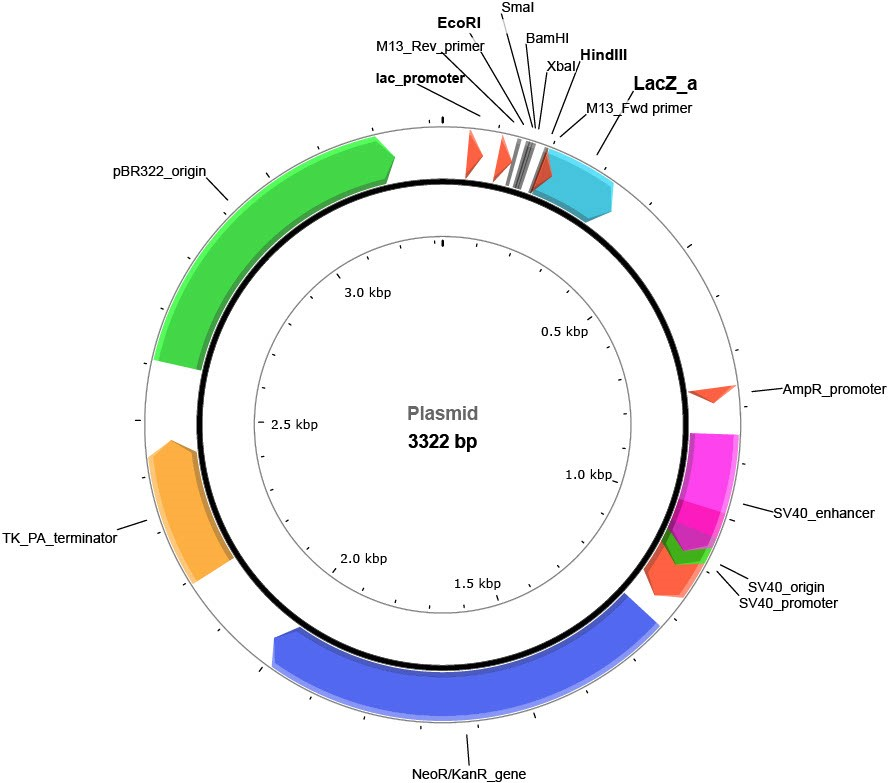
\includegraphics[width=10cm]{plasm1.jpg}
	\caption{pGGA\_Kan\_LacZ$\alpha$}
	\allikas{Autori andmed}
	\label{plasm}
\end{figure}

Kuna sellist plasmiidi ei olnud vastaval hetkel saada, konstrueeriti see ise. Selleks kasutati kanamütsiini resistentset plasmiidi pFA-CMV, mida lõigati restriktaasidega VspI ja AdeI. LacZ$\alpha$ järjestust sisaldavat plasmiidi pUC18 paljundati PCR reaktsioonis praimeritega BR322oriF ja LacZ$\alpha$-3Ade ning saadud produkti restrikteeriti samuti restriktaasidega VspI ja AdeI-ga. 450 nukletiidi pikkune fragment ligeeriti ettevalmistatud vektorisse ja transformeeriti \textit{Escherichia coli} tüvve DH5$\alpha$.
%Bakterikolooniad kasvatati \SI{15}{\milli\litre} LB-agarsöödet ja \SI{100}{\micro\gram\per\milli\litre} ampitsilliini, \SI{100}{\milli\mol} IPTG ning \SI{20}{\milli\gram\per\milli\litre} X-Gal sisaldavatel Petri tassidel.
Positiivsed kolooniad värvusid siniseks, neist eraldati plasmiidne DNA. Eraldatud plasmiidse DNA nukleotiidne järjestus kontrolliti sekveneerimisega, mille tulemus osutus soovituks. Nii saadi sinivalget selektsiooni võimaldav kanamütsiini resistentne plasmiid, mis sisaldas ka sobivaid EcoRI ja HindIII restriktsioonisaite (edaspidi nimetatud kui pGGA\_Kan\_LacZ$\alpha$) (Joonis \ref{plasm}).

\subsection{Fragmentide kloneerimine pGGA\_Kan\_LacZ$\alpha$ vektorisse}

%Tellitud plasmiidset DNA-d paljundati esmalt bakterites, seejärel tuli soovitud fragmentide eraldamiseks neid restrikteerida ning geelil tekkinud fragmendid üksteisest eraldada. Sobiva pikkusega fragmendid lõigati välja ja puhastati. Saadud DNA-d restrikteeriti koos valmistatud pGGA\_Kan\_LacZ$\alpha$ plasmiidiga restriktaasidega EcoRI ja HindIII. Pärast restriktsiooni ligeeriti fragmendid kokku ning transformeeriti saadud plasmiid \textit{Escherichia coli} tüvve DH5$\alpha$. Kontrolliks kasutati pGGA\_Kan\_LacZ$\alpha$ plasmiidi, mida restrekteeriti ja ligeeriti ilma inserteeritava plasmiidse DNA juuresolekuta.

Sünteetilised DNA plasmiidid Q1-Q8 transformeeriti kompetentsetesse
bakterirakkudesse (\textit{Escherichia coli} tüvi DH5$\alpha$) ning kasvanud kolooniatest eraldati plasmiidse DNA minipreparatsioonid. Eraldatud DNA-st restrikteeriti 1-2 \si{\micro\litre} restriktaasidega EcoRI ja HindIII ning tekkinud fragmendid lahutati üksteisest elektroforeesiga 1,5\% TAE-agaroosgeelil. Õiged fragmendid lõigati geelist välja ning neist puhastati DNA. Plasmiidist Q1 eraldati peptiidi uCendR ning AAV2 kapsiidi VR-VIII paremat ja vasakut
õlga kodeerivad DNA järjestused. Plasmiididest Q2 ja Q3 vastavalt peptiide LuS7A ja uEdbTnc kodeerivad DNA järjestused. Plasmiidist Q4 peptiidi abIntNRP ja AAV5 kapsiidi VR-IV paremat ja vasakut õlga kodeerivad DNA järjestused. Plasmiididest Q5-Q7 eraldati
vastavalt peptiide LuVG, IVEX1 ja LinTT1 ning plasmiidist Q8 peptiidi XBB1.5 ja AAV2 kapsiidi VR-IV paremat ja vasakut õlga kodeerivad DNA järjestused. Vektorit pGGA\_Kan\_LacZ$\alpha$ restrikteeriti samuti restriktaasidega EcoRI ja HindIII, tekkinud fragmendid lahutati geelelektroforeesil ning vektori \SI{3,3}{\kilo\base} suurune DNA fragment puhastati. Saadud vektori DNA-ga ligeeriti eraldi reaktsioonides kõik inserdid ning transformeeriti saadud ligeerimissegud \textit{E. coli} tüvve DH5$\alpha$. Negatiivseks kontrolliks kasutati sama vektorit – EcoRI-HindIII restrikteeritud pGGA\_Kan\_LacZ$\alpha$ plasmiidi, mida ligeeriti ning transformeeriti ilma inserteeritava fragmendi juuresolekuta.

\begin{figure}[htbp]
	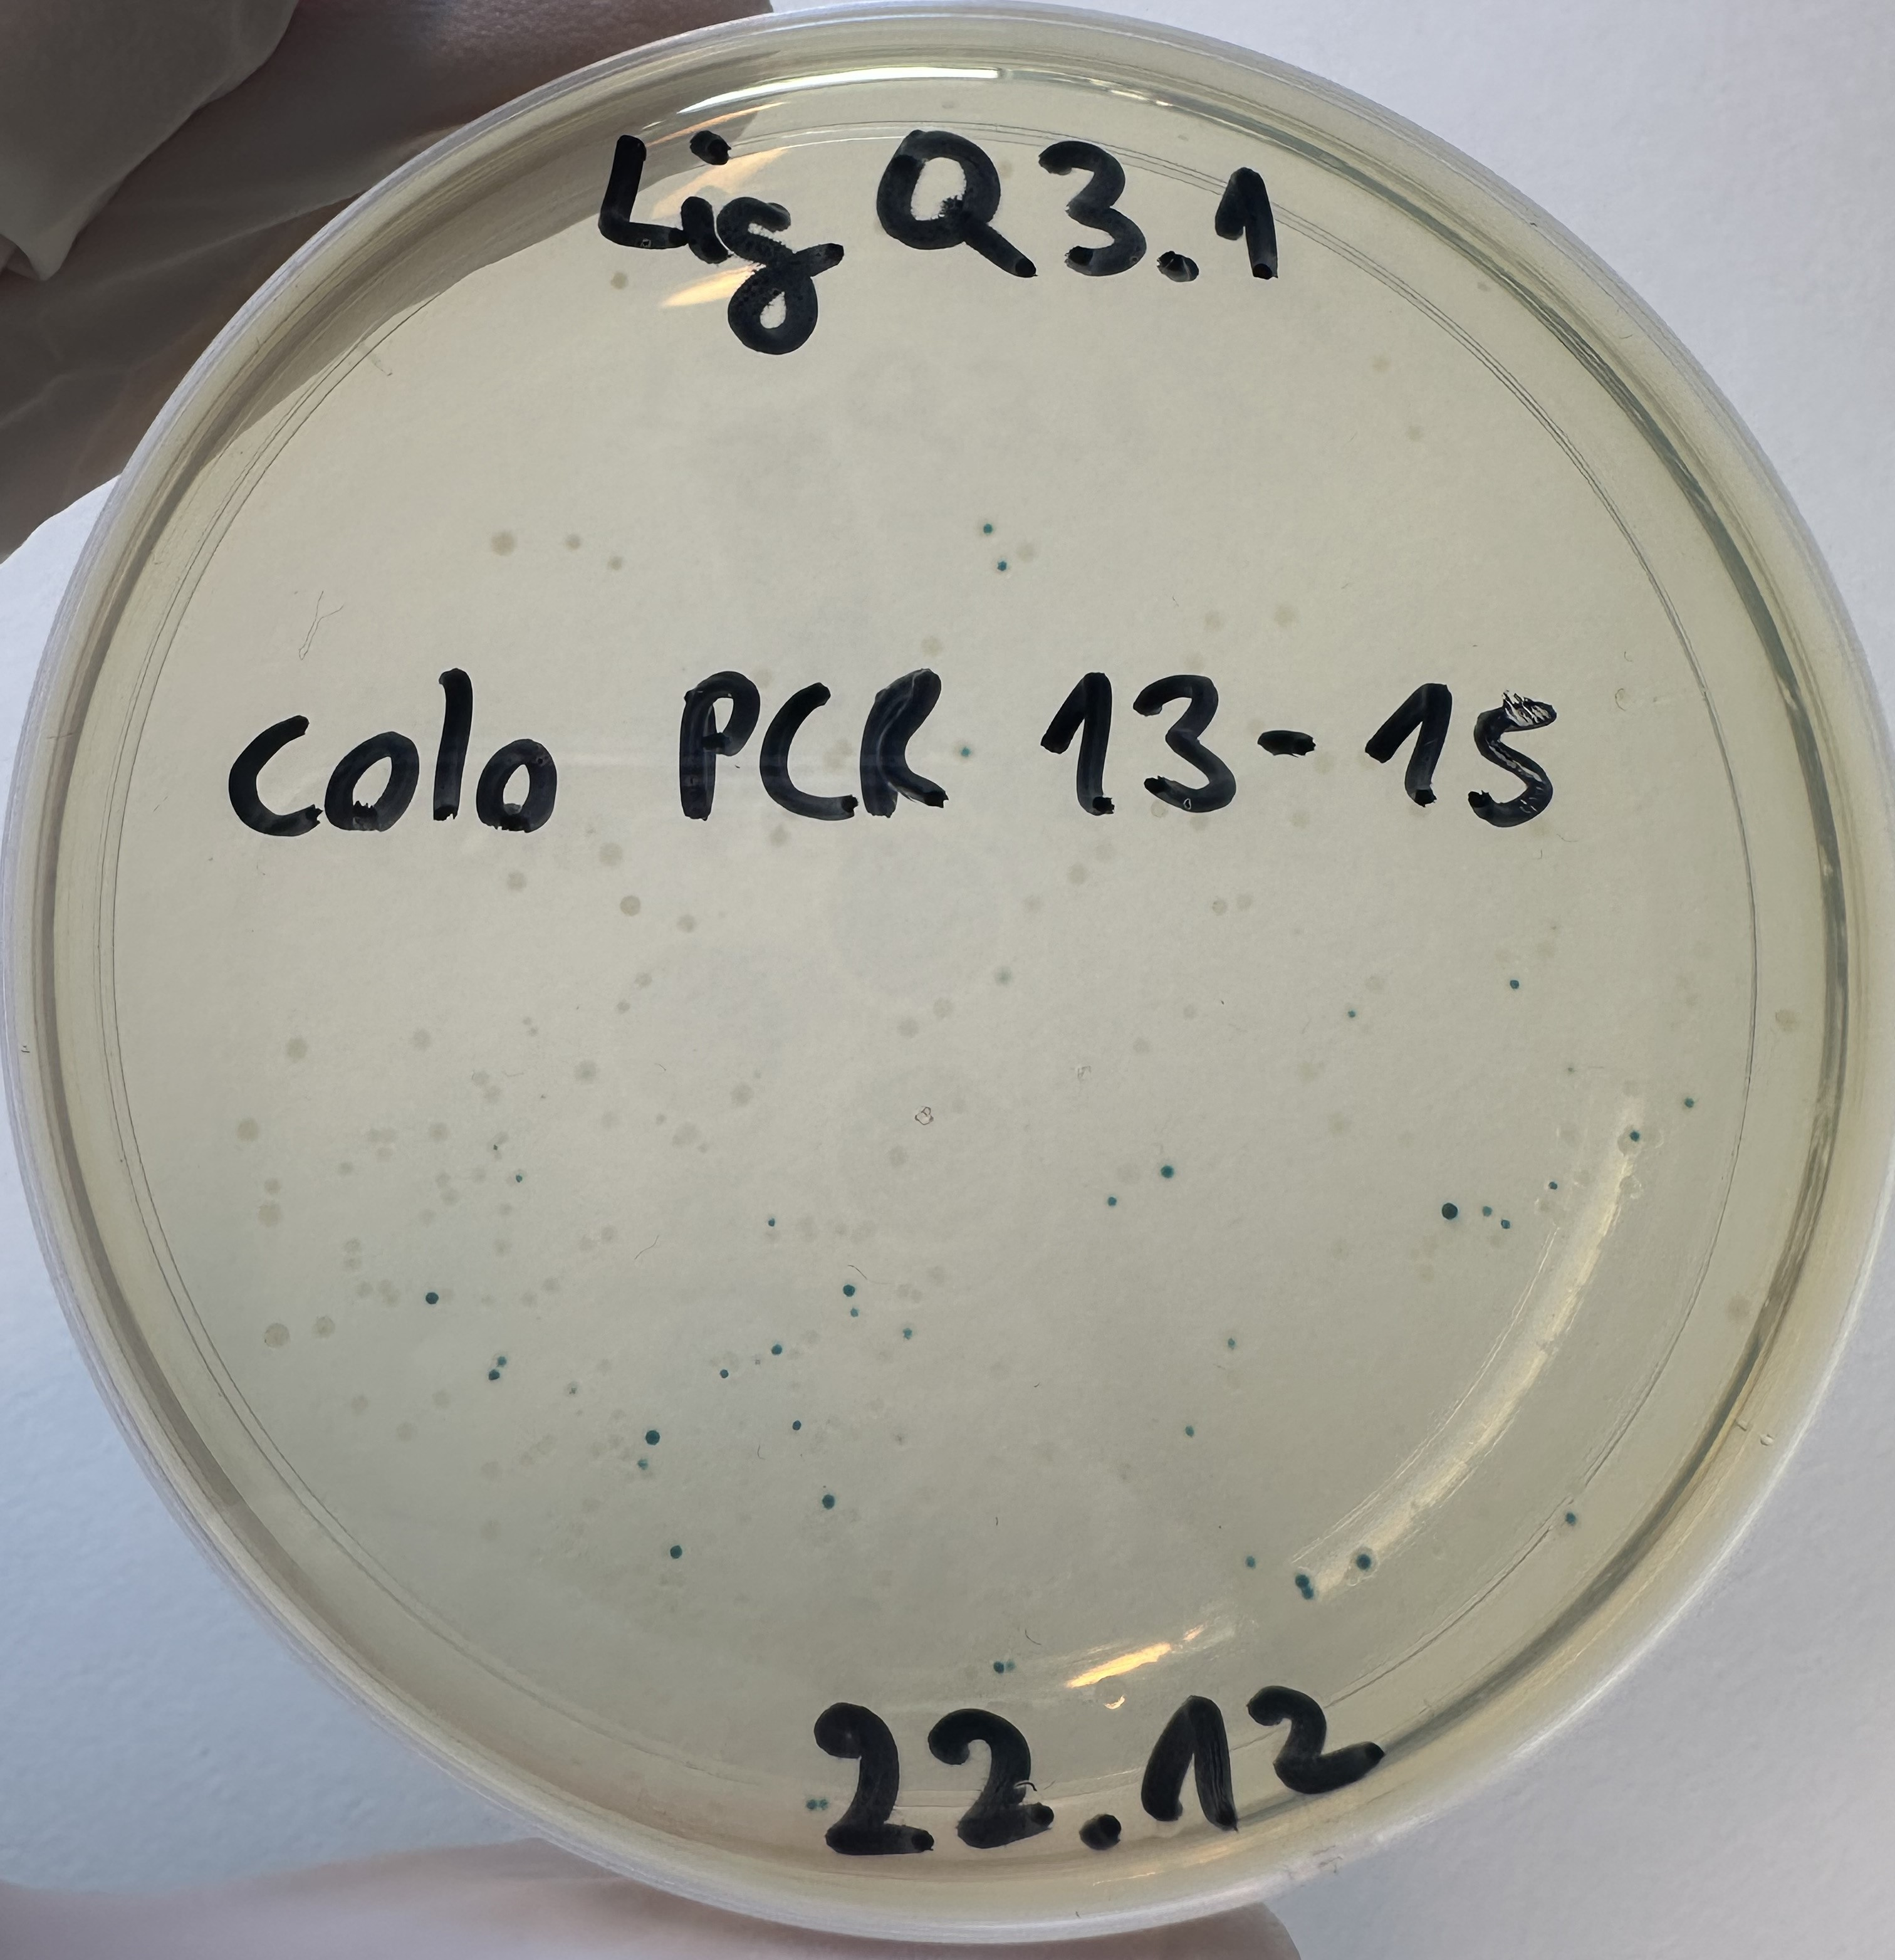
\includegraphics[width=7cm]{sinivalge.jpg}
	\caption{Sinised ja valged bakterikolooniad Petri tassil}
	\allikas{Autori andmed}
	\label{sinivalge}
\end{figure}

Tassidel, kus kasvasid inserdiga plasmiidi omavad bakterid, kasvas üles rohkem kui sada bakterikolooniat, negatiivsel kontrollil aga ainult paar. Üleskasvanud kolooniatest olid osad valged ja osad sinised (Joonis \ref{sinivalge}). Huvitav on märkida, et paljud õnnestunud ligeerimised andsid tulemuseks sinised kolooniad. Igalt tassilt eraldati kolm bakterikolooniat ja neile tehti koloonia PCR. Koloonia PCR-i produkte analüüsiti geelelektroforeesiga, mille abil kontrolliti inserdi suurust (Joonised \ref{colo1} ja \ref{colo2}). Sobivatest bakterikolooniatest eraldati plasmiidne DNA, mida seejärel sekveneeriti. Sekveneerimisel saadud DNA nukleotiidne järjestus osutus kõikide uuritud plasmiidide puhul ootuspäraseks, seega oldi saadud kõikide fragmentide jaoks BpiI restriktsioonisaitidega
varustatud plasmiidsed DNA konstruktid.

\begin{figure}[H]
	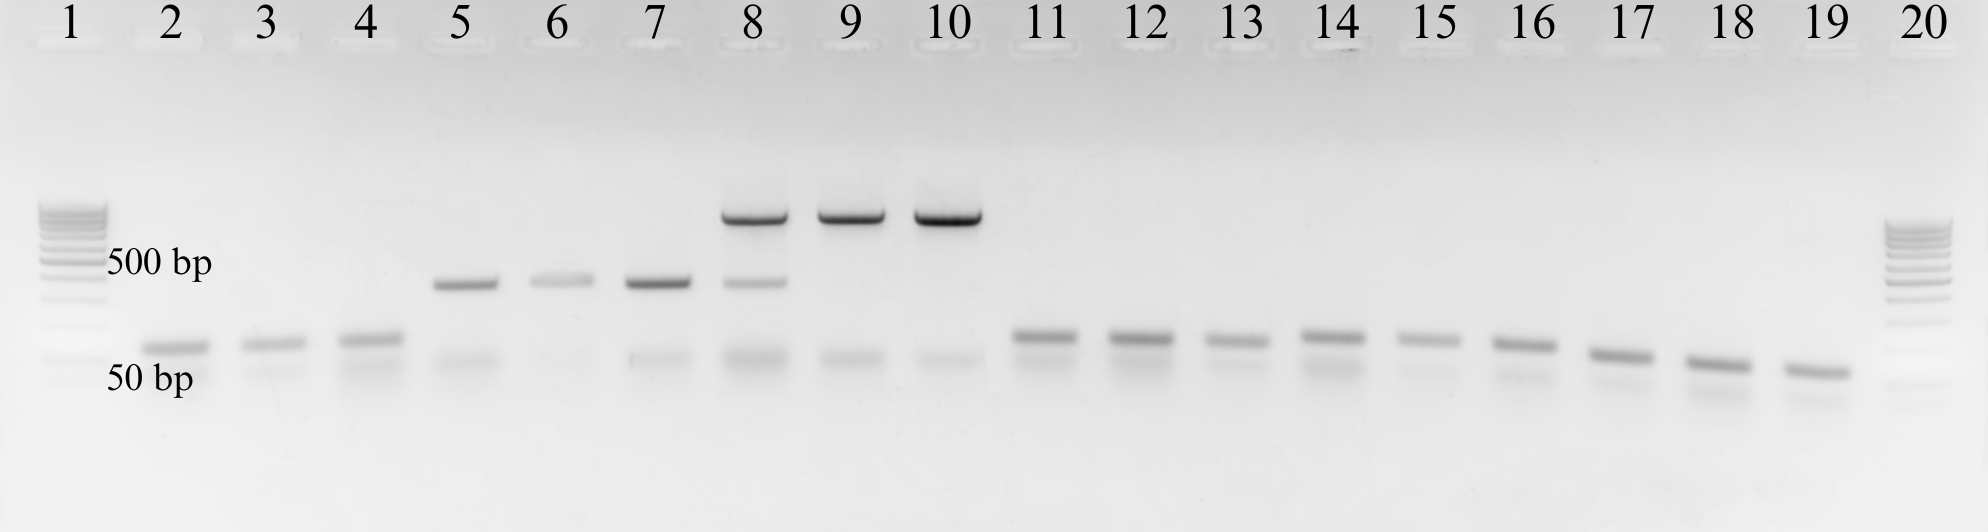
\includegraphics[width=14cm]{colopcr11.png}
	\caption{Bakterikolooniast tehtud PCR-i produktide analüüs geelelektroforeesil}
	\allikas{Autori andmed}
	\label{colo1}
\end{figure}

Joonisel \ref{colo1} on radadel 1 ja 20 50 aluspaari pikkune DNA-marker (GeneON). Ülejäänud radadel on inserdiga plasmiidid. Radadel 2-4 on inserdiks uCendR, 5-7 Cap2\_VR-VIII parem õlg, 8-10 Cap2\_VR-VIII vasak õlg, 11-13 LuS7A, 14-16 uEdbTncC ja radadel 17-19 $\alpha$v$\beta$3-Int-NRP1. Sekveneerimiseks valiti välja plasmiidid geelelektroforeesil saadud tulemuste põhjal: kolmest sama inserdiga plasmiidist eelistati kõige kõrgema kontsentratsiooni ja korrektse pikkusega plasmiidi. Valituteks osutusid plasmiidid, mille PCR produkte analüüsiti radadel 2, 5, 10, 11, 14 ja 17.

\begin{figure}[H]
	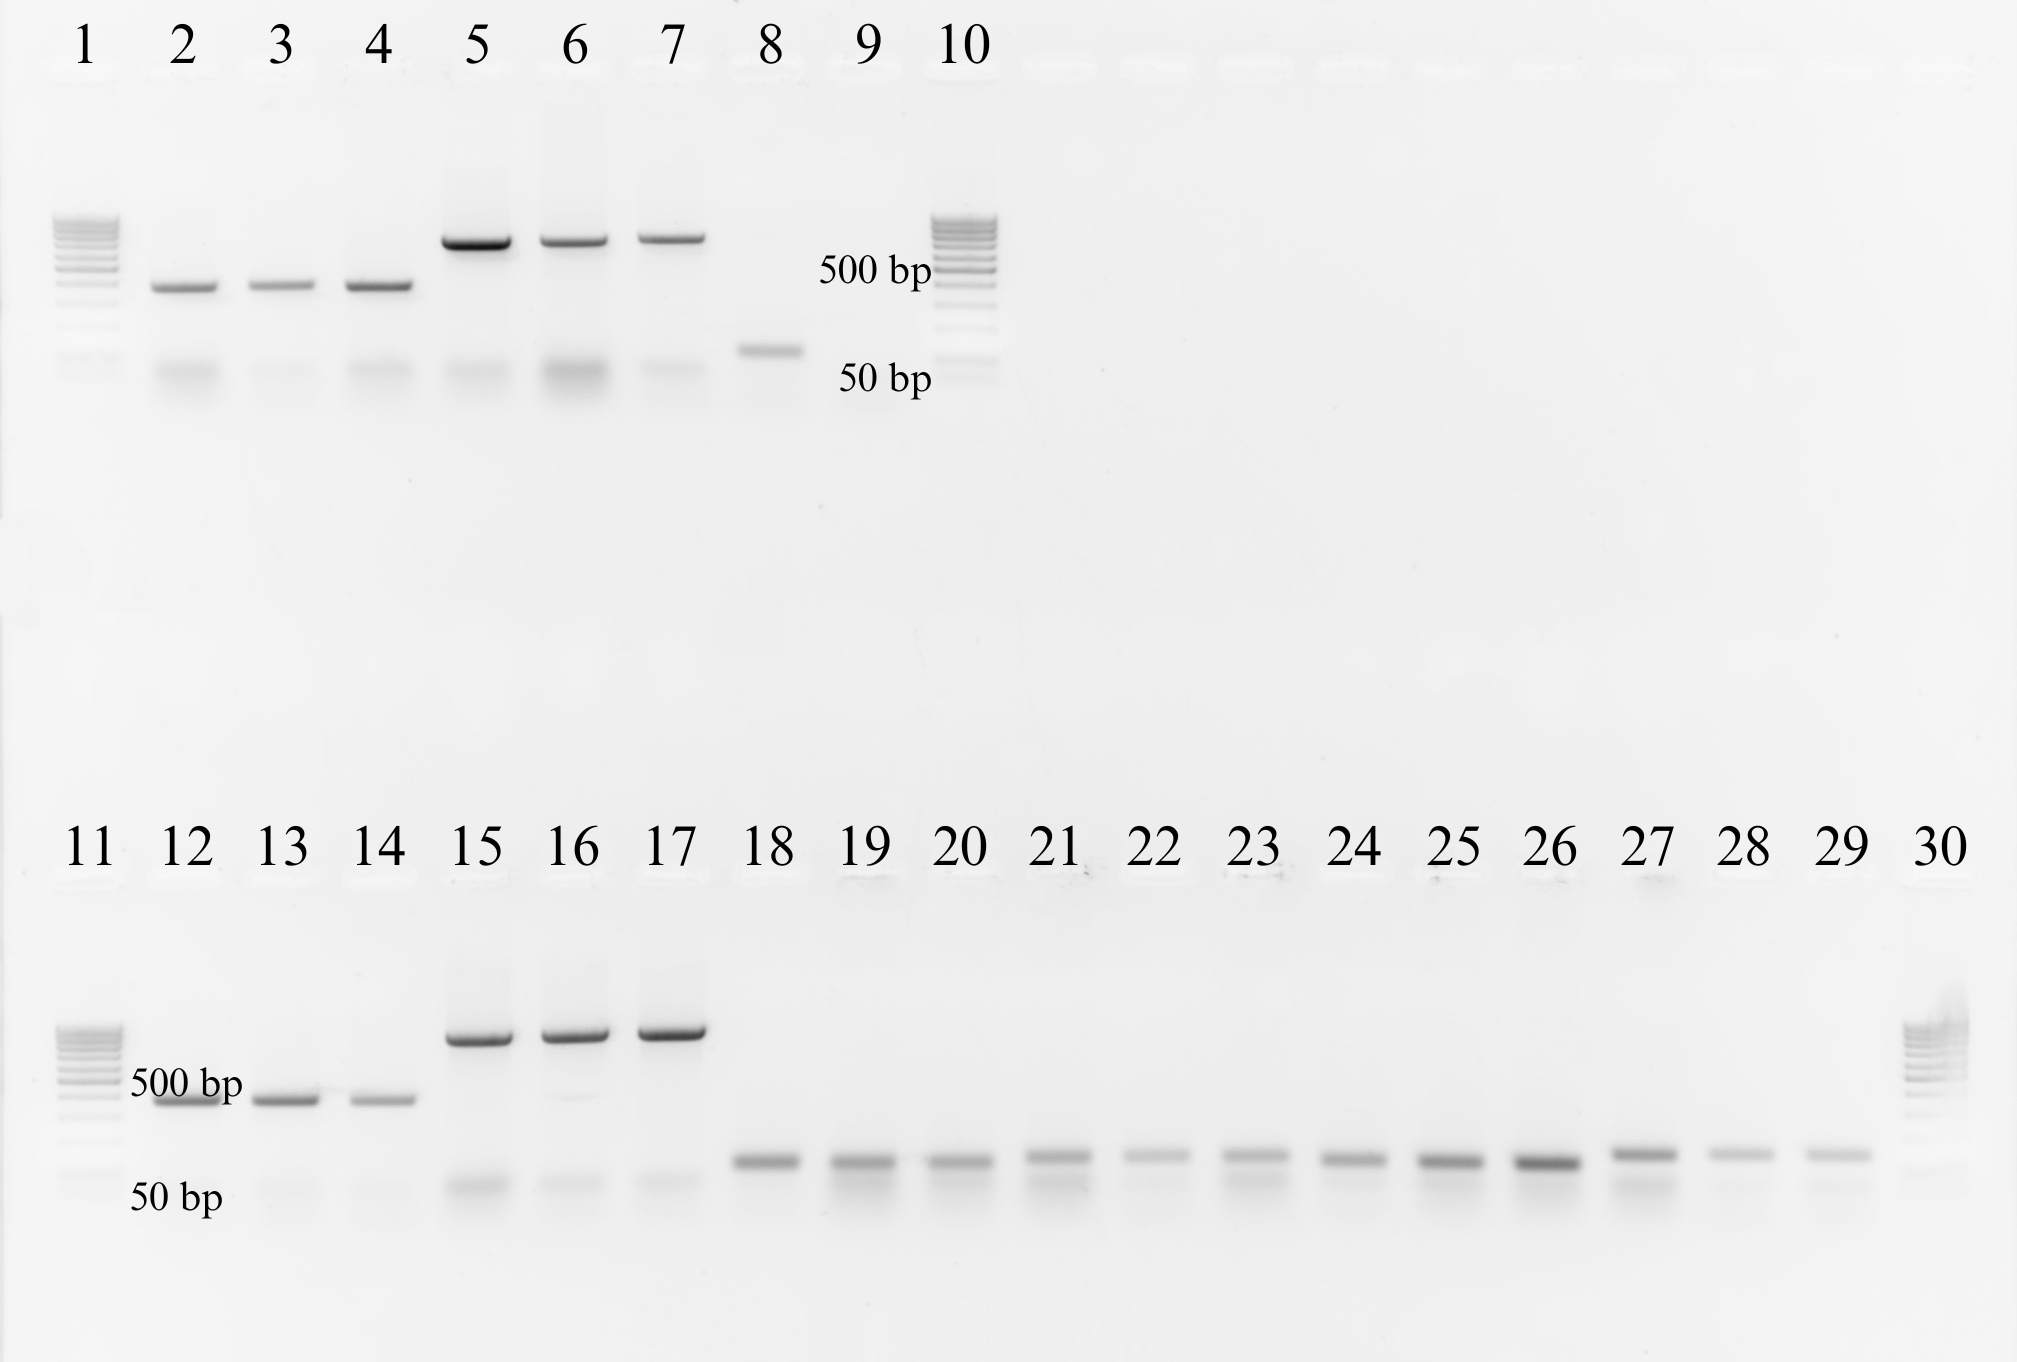
\includegraphics[width=14cm]{colopcr21.png}
	\caption{Bakterikolooniast tehtud PCR-i produktide analüüs geelelektroforeesil}
	\allikas{Autori andmed}
	\label{colo2}
\end{figure}

Joonisel \ref{colo2} on radadel 1, 10, 11 ja 30 50 aluspaari pikkune DNA-marker (GeneON). Rajal 8 on positiivseks kontrolliks \SI{50}{\basepair} pikkuse inserdiga plasmiid ja rajal 9 negatiivseks kontrolliks PCR-i segu, millele pole baktereid lisatud. Ülejäänud radadel on inserdiga plasmiidid. Radadel 2-4 on inserdiks Cap2\_VR-IV vasak õlg, 5-7 Cap2\_VR-IV parem õlg, 12-14 Cap5. VR-IV vasak õlg, 15-17 Cap5. VR-IV parem õlg, 18-20 LuVG, 21-23 IVEX1, 24-26 LinTT1 ja radadel 27-29 XBB1.5. Sekveneerimiseks valiti geelipildi alusel välja plasmiidid, mille PCR produkte analüüsiti radadel 2, 5, 12, 15, 18, 21, 24 ja 27.

\subsection{Golden Gate kloneerimine}

Edasi kloneeriti lühendatud AAV2 ja AAV8 kapsiidiplasmiididesse eeldatavalt kopsukoe ja vähkkasvaja spetsiifilised peptiidid, kasutates Golden Gate metoodikat. Kokku kloneeriti AAV lühendatud plasmiidid, muutuvpiirkondade vasakut ja paremat õlga kodeerivad plasmiidid ning sisestatavat peptiidi kodeeriv plasmiid. Kokku valmis 20 erinevat lühendatud AAV kapsiidiplasmiidi (Tabel \ref{ggtabel}).

Doonorplasmiidid olid varustatud vajalike BpiI restriktsioonisaitidega, kuid lühendatud AAV2 ja AAV8 kapsiidiplasmiidid neid ei sisaldanud. Seega aktseptoreid eelnevalt restrikteeriti sobivate restriktaasidega, fragmendid puhastati geelist ja nende DNA segati õiges stöhhiomeetrilises vahekorras Golden Gate reaktsioonisegusse. Peale transformatsiooni ja kolooniate üleskasvamist eraldati plasmiidne DNA, iga kloneerimise kohta kasutati 2-3 kolooniat, millest ühel määrati inserdi järjestus sekveneerimisega. Kõik analüüsitud plasmiidid osutusid ootuspäraseks.

\begin{table}[H]
\caption{Golden Gate meetodil kokku kloneeritud fragmendid}
\label{ggtabel}
\begin{tabular}{|p{3cm}|p{3cm}|p{3cm}|}
	\hline
	Aktseptor & Sisestuskoht & Peptiid \\
	\hline
	\centering\multirow{16}{*}{\Large{Cap2}} & \centering\multirow{8}{*}{VR-IV} & \footnotesize{uCendR} \\
	& & \footnotesize{XBB1.5} \\
	& & \footnotesize{LuS7A} \\
	& & \footnotesize{uEdbTncC} \\
	& & \footnotesize{$\alpha$v$\beta$3-Int-NRP1} \\
	& & \footnotesize{LuVG} \\
	& & \footnotesize{IVEX1} \\
	& & \footnotesize{LinTT1} \\
	\cline{2-3}
	& \centering\multirow{8}{*}{VR-VIII} & \footnotesize{uCendR} \\
	& & \footnotesize{XBB1.5} \\
	& & \footnotesize{LuS7A} \\
	& & \footnotesize{uEdbTncC} \\
	& & \footnotesize{$\alpha$v$\beta$3-Int-NRP1} \\
	& & \footnotesize{LuVG} \\
	& & \footnotesize{IVEX1} \\
	& & \footnotesize{LinTT1} \\
	\hline
	\centering\multirow{4}{*}{\Large{Cap8}} & \centering\multirow{2}{*}{VR-IV} & \footnotesize{uCendR}\\
	& & \footnotesize{XBB1.5} \\
	\cline{2-3}
	& \centering\multirow{2}{*}{VR-VIII} & \footnotesize{uCendR}
	\\
	& & \footnotesize{XBB1.5} \\
	\hline
	\end{tabular}
\allikas{Autori andmed}
\end{table}

\begin{comment}
\begin{table}[htb]
	\caption{Golden Gate meetodil kokku kloneeritud fragmendid}
	\label{ggtael}
	\begin{tabular}{ |p{3cm}|p{3cm}|p{3cm}|p{3cm}|}
		\hline
		Aktseptor & Insertsiooni koht & Peptiid & Parem õlg \\
		\hline
		\centering\multirow{16}{*}{\Large{Cap2}} & \centering\multirow{8}{*}{\large{IV}} & \footnotesize{uCendR} & \centering\arraybackslash\multirow{8}{*}{\large{IV}} \\
		& & \footnotesize{XBB1.5} & \\
		& & \footnotesize{LuS7A} & \\
		& & \footnotesize{uEdbTncC} & \\
		& & \footnotesize{$\alpha$v$\beta$3-Int-NRP1} & \\
		& & \footnotesize{LuVG} & \\
		& & \footnotesize{IVEX1} & \\
		& & \footnotesize{LinTT1} & \\
		\cline{2-4}
		& \centering\multirow{8}{*}{\large{VIII}} & \footnotesize{uCendR} & \centering\arraybackslash\multirow{8}{*}{\large{VIII}} \\
		& & \footnotesize{XBB1.5} & \\
		& & \footnotesize{LuS7A} & \\
		& & \footnotesize{uEdbTncC} & \\
		& & \footnotesize{$\alpha$v$\beta$3-Int-NRP1} & \\
		& & \footnotesize{LuVG} & \\
		& & \footnotesize{IVEX1} & \\
		& & \footnotesize{LinTT1} & \\
		\hline
		\centering\multirow{4}{*}{\Large{Cap8}} & \centering\multirow{2}{*}{\large{IV}} & \footnotesize{uCendR} & \centering\arraybackslash\multirow{2}{*}{\large{IV}} \\
		& & \footnotesize{XBB1.5} & \\
		\cline{2-4}
		& \centering\multirow{2}{*}{\large{VIII}} & \footnotesize{uCendR} & \centering\arraybackslash\multirow{2}{*}{\large{VIII}} \\
		& & \footnotesize{XBB1.5} & \\
		\hline
	\end{tabular}
	\allikas{Autori andmed}
\end{table}
\end{comment}


\subsection{Peptiididega modifitseeritud täispikkade pRepCap plasmiidide	konstrueerimine}

Golden Gate kloneerimise tulemusena saadi plasmiidid, mis sisaldasid küll peptiididega modifitseeritud kapsiide kodeerivaid järjestusi, kuid kapsiidid ise olid lühendatud. Edasi kloneeriti need täispikka kapsiidi kodeerivasse plasmiidi: Cap2 järjestused kloneeriti
plasmiidi pRC2 ja Cap8 järjestused plasmiidi pAAV2/8. Selleks restrikteeriti Cap2 plasmiide restriktaasidega Pfl23II ja NheI ning Cap8 plasmiide restriktaasidega Pfl23II ja NotI, õiged fragmendid puhastati geelist ja sisestati täispikkade plasmiidide vastavatesse restriktsioonisaitidesse. Kõigilt transformeeritud tassidelt eraldati kahe bakterikoloonia plasmiidne DNA ning analüüsiti täispikki pRepCap plasmiide geelelektroforeesil.

%Golden Gate kloneerimisest saadud lühendatud plasmiidne DNA kloneeriti täispikka kapsiidi kloneerivasse plasmiidi. Cap2. lühendatud plasmiidi kloneeriti täispikka plasmiidi pRC2 ja Cap8. lühendatud plasmiidi kloneeriti täispikka plasmiidi pAAV2/8. Selleks restrekteeriti Cap2. plasmiide restriktaasidega PH23 ja NheI ning Cap8. plasmiide restriktaasidega PH23 ja Not. Restriktsioonile järgnes ligeerimine ja DNA transformeerimine bakteritesse. Kõigilt transformeeritud tassidelt eraldati kahe bakterikoloonia plasmiidne DNA ning analüüsiti täispikki pRepCap plasmiide geelelektroforeesil.

\begin{figure}[H]
	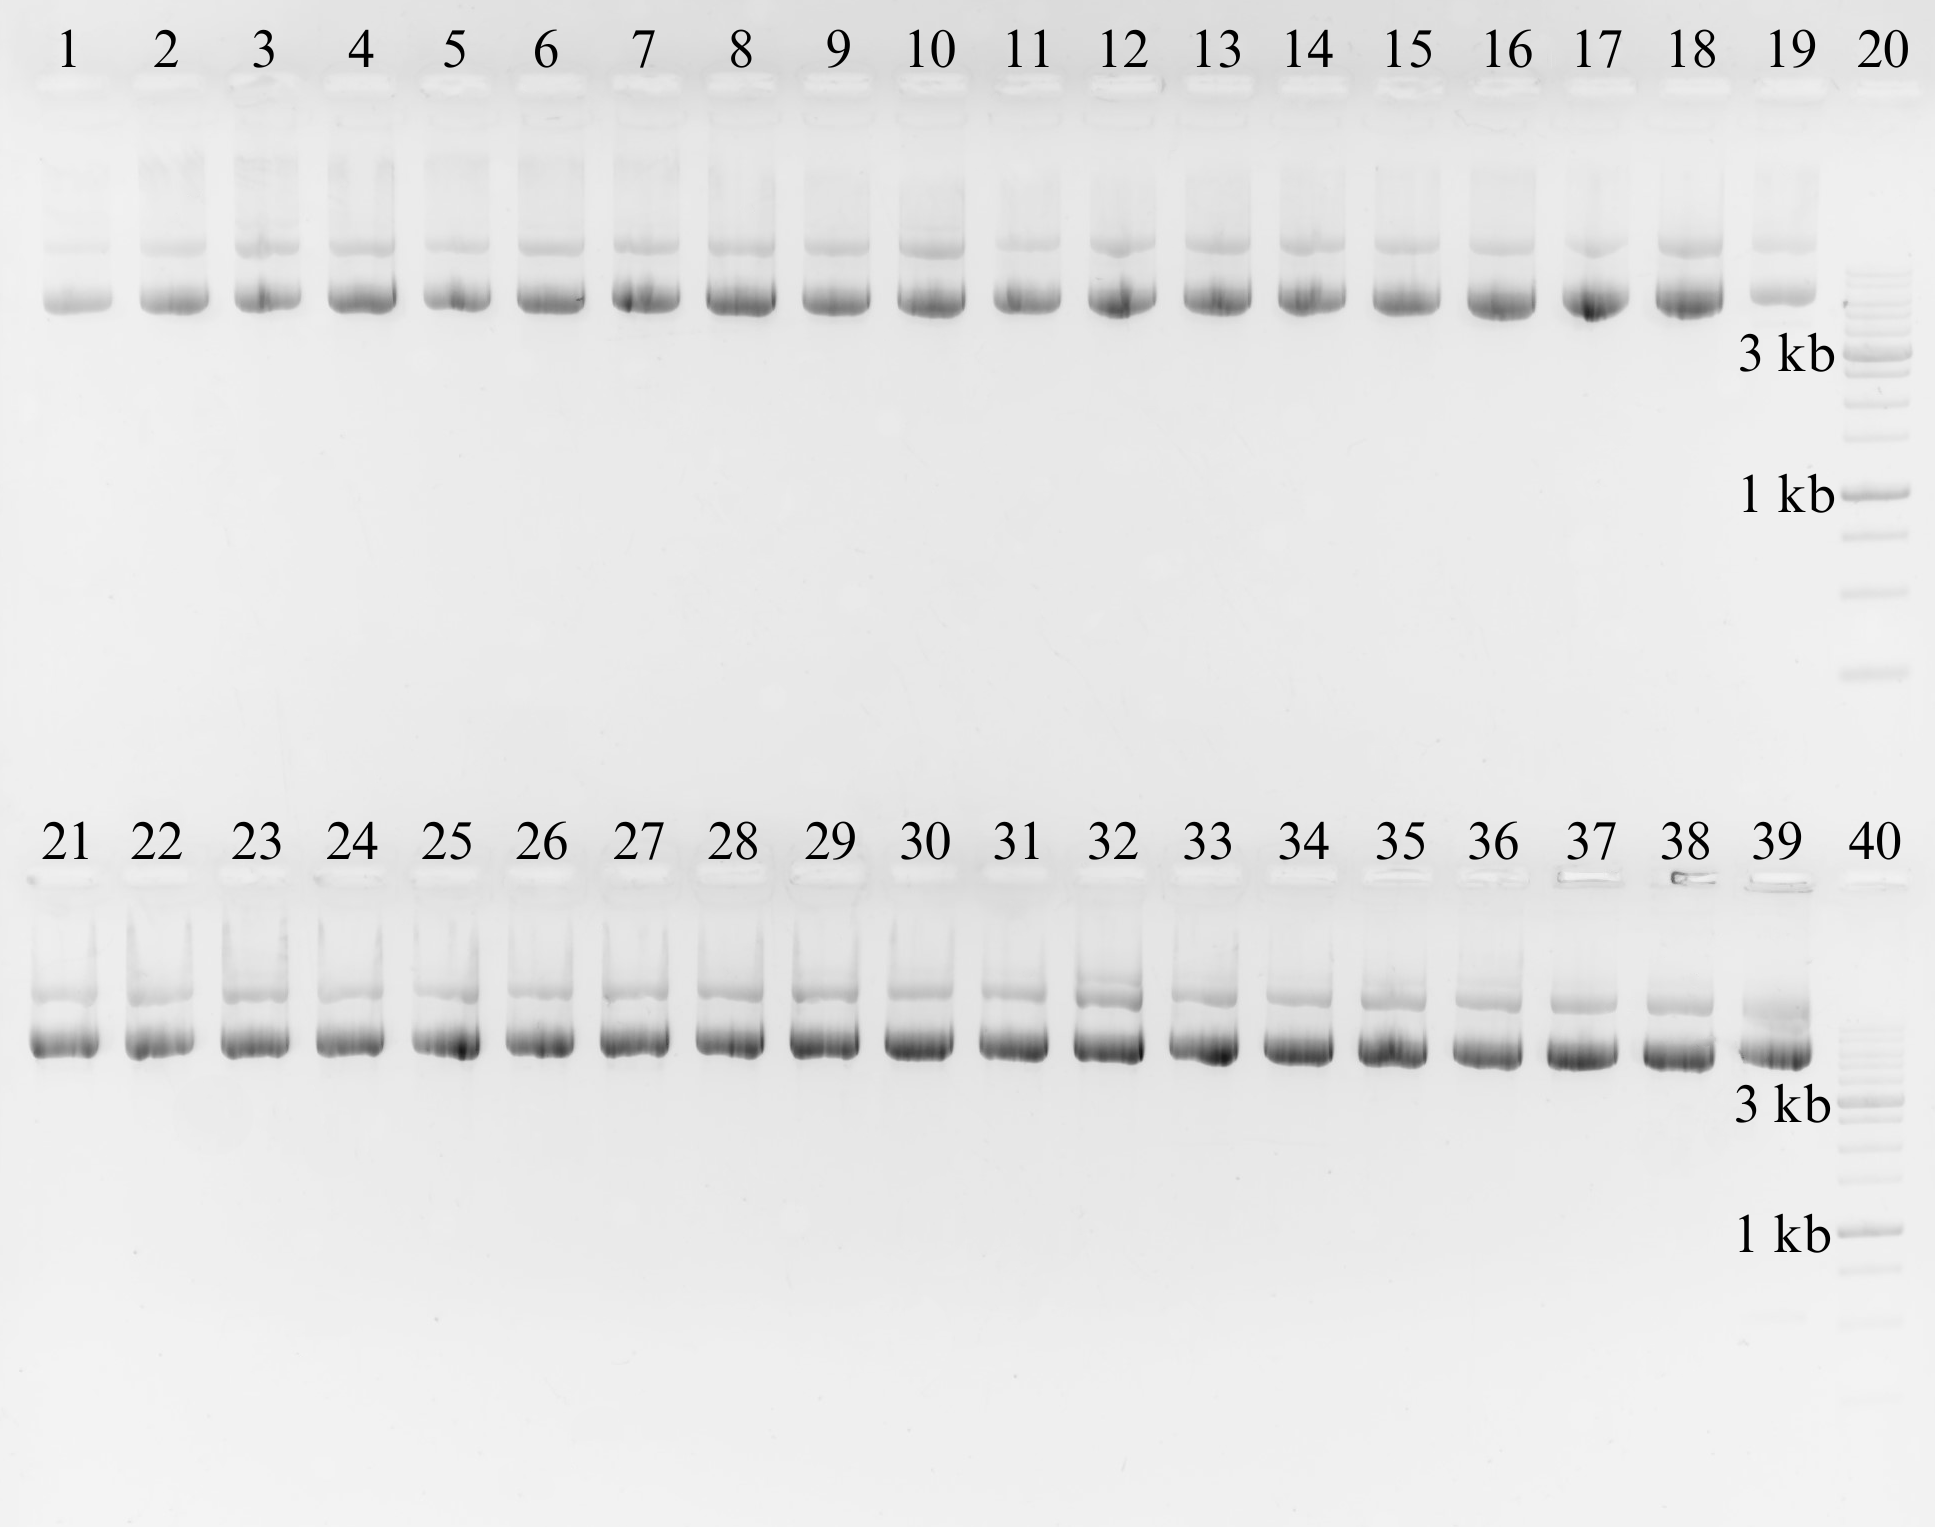
\includegraphics[width=14cm]{ggfull.png}
	\caption{Täispikkade pRepCap plasmiidide analüüs geelelektroforeesil}
	\allikas{Autori andmed}
	\label{ggfull}
\end{figure}

Joonisel \ref{ggfull} on radadel 20 ja 40 \SI{1}{\kilo\base} DNA-marker (Solis BioDyne). Rajal 19 on võrdluseks inserdita pAAV2/8 ja rajal 39 inserdita pRC2. Radadel 1-10, 23-24 ja 37-38 on pRC2, milles on inserdiks Cap2\_VR-VIII, millesse on sisestatud peptiidid. Radadel 1 ja 2 on peptiidiks uEdbTncC, 3 ja 4 $\alpha$v$\beta$3-Int-NRP1, 5 ja 6 LuVG, 7 ja 8 IVEX1, 9 ja 10 LinTT1, 23 ja 24 uCendR ning radadel 37 ja 38 LuS7A. Radadel 21-22 ja 25-36 on pRC2, milles on inserdiks Cap2\_VR-IV, millesse on sisestatud peptiidid. Radadel 21 ja 22 on peptiidiks XBB1.5, 25 ja 26 LuS7A, 27 ja 28 uEdbTncC, 29 ja 30 $\alpha$v$\beta$3-Int-NRP1, 31 ja 32 LuVG, 33 ja 34 IVEX1 ning radadel 35 ja 36 LinTT1. Radadel 11-18 on inserdiks lühendatud Cap8 plasmiidid. Radadel 11 ja 12 sisaldub inserdis VR-IV sisestatud uCendR, 13 ja 14 VR-IV sisestatud XBB1.5, 15 ja 16 VR-VIII sisestatud uCendR ja radadel 17 ja 18 VR-VIII sisestatud XBB1.5. Geelipildilt on näha, et peptiide sisaldavate kapsiidivariantide viimine täispikkadesse plasmiididesse läks ootuspäraselt.

\subsection{Tõhusamate Golden Gate aktseptorplasmiidide konstrueerimine}

Golden Gate metoodika edaspidiseks hõlpsamaks rakendamiseks otsustati
aktseptorfragmendid asendada plasmiididega, kus sobivad üleulatuvad otsad tekiksid restriktaas BpiI lõikamise tulemusena. Sellisel juhul pole vaja enam aktseptorfragmente eraldi plasmiididest puhastada, mis on äärmiselt töömahukas. Selle asemel piisab vaid õigete Golden Gate
plasmiidide kokkusegamisest. Selleks telliti oligonukleotiidpraimerid, millesse disainiti sobivad BpiI restriktsioonisaidid. Lisaks sisaldab praimer 5’ otsas HindIII restriktsioonisaiti, et tekkinud PCR-i produkti oleks mugav plasmiidirõngaks ligeerida. See osa projektist on praegu kloneerimise staadiumis.

%Golden Gate metoodika edaspidiseks hõlpsamaks rakendamiseks otsustati aktseptorfragment asendada nagu doonorplasmiididki ampitselliini resistentsete plasmiididega. Selleks telliti oligonukleotiidpraimerid, millesse disainiti BpiI restrektsioonisait, mille lõikamise tulemusena tekiksid sobivad üleulatuvad otsad. Lisaks sisaldab praimer 5' otsas HindIII restrektsioonisaiti, et tekkinud PCR-i produkti oleks mugav plasmiidirõngaks ligeerida. 

\subsection{AAV transduktsiooni võime mõõtmine koekultuuri rakkudes}

AAV viirusvektori tootmise testimiseks valiti kapsiidid AAV2\_IV-uCendR ja AAV2\_VIII-uCendR ning kontrolliks kasutati metsiktüüpi AAV2 kapsiidi. Niinimetatud genoomseks ehk transgeeni plasmiidiks kasutati jaanimardika lutsiferaasi püsivalt ekspresseerivat AAV konstrukti (IVEX Lab, plasmiid nr 745). Viirusvektori tootmisprotsessi käigus rakukultuuris ei olnud märgata erinevusi metsiktüüpi ja uCendR peptiide kandvate kapsiidide vahel. Edasi nakatati HEK293FT rakke puhastatud viirusvektoritega, kasutades viirusvektori neljakordset lahjenduste rida, alates \SI{0,004}{\micro\litre} kuni \SI{4}{\micro\litre} viirusvektorit ühe kannu kohta 96-kannulises koekultuuriplaadis.


\begin{figure}[htbp]
	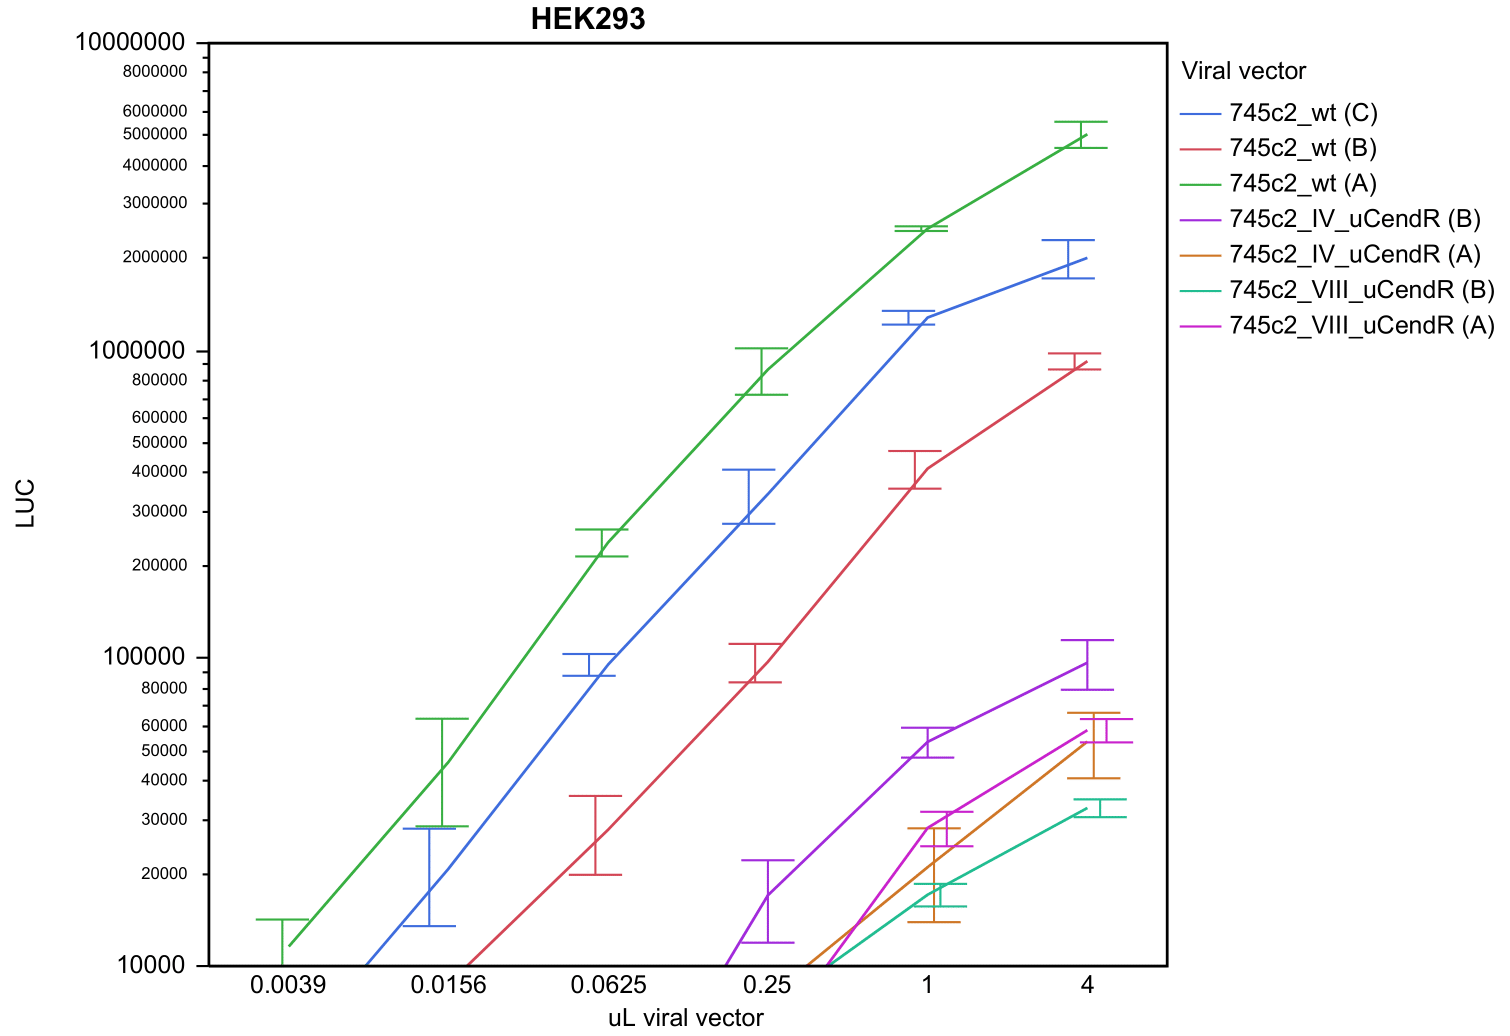
\includegraphics[width=13cm]{Log HEK293.png}
	\caption{LUC aktiivsus rakuliinis HEK293 erinevate kapsiidivariantide puhul}
	\allikas{Autori andmed}
	\label{log}
\end{figure}

Viis päeva hiljem mõõdeti rakkudes lutsiferaasi aktiivsus ehk luminestsentsi. Tulemused on esitatud joonisel \ref{log}. A, B ja C märgised vektorite juures tähistavad sama vektori tootmise kordusi. uCendR insertsiooniga viirusvektoritega mõjutatud rakud andsid 50-100 korda madalamad luminestsentsi väärtused kui metsiktüüpi AAV2 kontrollviirused.

\section{Arutelu}

%Hästi kasutatav Golden Gate doonorvektor pGGP\_ sisaldab populaarse pUC18 vektori polülinkerit, mis võimaldab kloneerimisel kasutada levinud restriktaase, ning LacZ$\alpha$ ekspressioonikassetti, mis võimaldab sini-valget selektsiooni. Kõikide fragmentide kloneerimisel ligeerimissegu transformeerimisel tekkis selle vektoriga kümneid kordi rohkem positiivseid kolooniaid kui negatiivses kontrollis. Varasemalt on samas projektis esinenud suuri problobleeme insertide sisestamisega Kanamütsiini resistentsesse vektorisse. Uue Golden Gate doonorvektoriga on need probleemid lahendatud. Mitmel juhul värvusid aga ka positiivsed kolooniad siniseks, justkui oleksid need olnud inserdita plasmiidid. Nimelt olid mitmed kloneeritavad fragmendid lühikesi peptiide kodeerivad järjestused, mille lisamine EcoRI-HindIII sisestus kohtadesse ei põhjustanud LacZ$\alpha$ lugemisraamis nihet või stoppkoodoni teket. Ka Cap5\_VR-IV vasaku õla inserdiga, mis oli \SI{400}{\basepair} pikk, plasmiide sisaldavad kolooniad värvusid siniseks.

Käesoleva töö raames valminud Golden Gate doonorvektor pGGD\_Kan\_LacZ$\alpha$ osutus tõhusaks kloneerimisvektoriks - kõikide fragmentide kloneerimisel tekkis selle vektoriga ligeerimissegu transformeerimisel kümneid kordi rohkem kolooniaid kui negatiivses kontrollis. Antud vektor sisaldab populaarse pUC18 vektori polülinkerit, mis võimaldab kloneerimisel kasutada EcoRI ja HindIII kõrval ka teisi levinud restriktaase, ning LacZ$\alpha$ ekspressioonikassetti, mis võimaldab sinivalget selektsiooni. Varasemalt on samas projektis esinenud suuri probleeme insertide sisestamisega kanamütsiini resistentsesse vektorisse. Uue Golden Gate doonorvektoriga on need mured lahendatud. Huvitav on märkida, et mitmel juhul värvusid ka positiivsed kolooniad siniseks, justkui oleksid need olnud inserdita plasmiidid. See on mõistetav, kuna suur osa kloneeritavatest fragmendist olid lühikesi peptiide kodeerivad järjestused, mille lisamine EcoRI-HindIII sisestuskohtadesse ei põhjustanud stoppkoodoni teket ja LacZ$\alpha$ inaktsivatsiooni. Kuna kloneerimine toimus kõrge efektiivsusega, siis sinivalge selektsioon ei osutunud kriitiliseks. 

%Tähtis on, et on valminud AAV kapsiidide modifitseerimise platvorm, millele on edaspidi lihtne lisada uusi komponente.

Ka Golden Gate metoodika rakendamine oli edukas: kõik peptiidid õnnestus valitud AAV kapsiidipiirkondadesse sisestada ning sekveneerimistulemuste järgi olid saadud konstruktid ilma mutatsioonideta ehk korrektsed. Kõik modifitseeritud kapsiidid on ka kloneeritud täispikkadesse pRepCap plasmiididesse, kokku on valminud selle uurimistöö raames 20 uut peptiidi insertsiooniga serotüüpi, 16 neist on modifitseeritud AAV2 kapsiidid ja neli modifitseeritud AAV8 kapsiidid. Golden Gate näol on valminud AAV kapsiidide modifitseerimise platvorm, millele on edaspidi võimalik lisada kerge vaevaga üha uusi komponente, ning neid omavahel kombineerides saada mahukas modifitseeritud AAV kapsiidivariantide raamatukogu.

Antud katsetes kasutati Golden Gate aktseptorplasmiidina tavapärasel meetodil restrikteeritud ja geelist puhastatud DNA fragmente, mis pärinesid AAV2 ja AAV8 lühendatud kapsiidiplasmiididest. Töö käigus leiti, et mugavam oleks ka aktseptorplasmiidid Golden Gate platvormile viia, sel juhul tekiks ka aktseptorvektori üleulatuvad otsad IIS tüüpi restriktaasidega lõikamise tulemusel. Nii saaks Golden Gate reaktsiooni tegemiseks lihtsalt kokku segada kõik vajalikud plasmiidsed DNA-d ja ensüümid, ilma eelneva vektorifragmendi puhastamiseta. AAV2, AAV5, AAV8 ja AAV9 kapsiidiplasmiidide vastav muutmine on praegu töös.
 
%muutmiseks on disainitud PCR praimerid, mis sisaldavad BpiI lõikamiskohti koos sobivate üleulatuvate järjestustega. Hetkel on sobivate aktseptorplasmiidide loomise projekt töös.

Viirusvektorite proovitootmine viidi läbi uCendR-sisaldavaid AAV2 kapsiide kasutades, pakkides lutsiferaasi ekspresseerivat AAV genoomi. Kuna võrreldes kontrolliga, milleks kasutati metsiktüüpi AAV2 kapsiidi, ei ilmnenud tootjarakkudes erinevusi metsiktüüpi ja uCendR-kapsiidide vahel, võib järeldada, et uCendR järjestused kapsiidis ei ole ekspressioonis rakkudele toksilised. See on oluline teave, vastasel juhul oleks neid viirusvektoreid rakkudes keerukas toota. Saadud preparaatide transduktsioonivõime testimisel HEK293FT rakkudes aga ilmnes, et uCendR insertsiooni omavad viirused andsid rakkudel 50-100 korda madalamad luminestsentsiväärtused kui metsiktüüpi kapsiidiga AAV2. Selle põhjus võib olla kas uCendR-viiruste madalam nakatamisvõime HEK293FT rakkudes või nende viiruste madalamad saagised tootmises. Põhjuste kindlaks määramiseks on edaspidi kavas mõõta iga viiruse preparaadi tiiter ehk AAV genoomi koopiate arv mahuühikus kvantitatiivse PCR-ga, ning uurida eri viiruste nakatamisvõimet ka teistes, kopsukoest ja eri kasvajatest pärit rakuliinides. Kirjeldatud katseid on vaja korrata kõikide loodud AAV kapsiidivariantidega. 

Kuna viimastel aastatel on kopsufibroosi põdejate hulk kiiresti kasvanud seoses COVID-19 pandeemiaga ning kopsude ja kasvajate ravivõimalused on hetkel kasinad, on projektis tehtavad peptiidsed muudatused väga aktuaalsed. Projekti jätkumisel loodetakse luua uudseid kopsu ja vähispetsiifilisi viirusvektoreid, mis parandaksid toodud haiguste ravi väljavaateid.

%Valitud peptiidsed modifikatsioonid, mis on selles töös AAV kapsiididesse sisse viidud, esindavad kopsukude ja kasvajaid sihtivaid järjestusi, sest nende ravivõimalused on praegu kasinad. 

%Leiti, et mugavam on viia ka aktseptorplasmiidid Golden Gate platvormile (s.t. sobivad üleulatuvad otsad tekivad samuti tüüp IIS restriktaasi(de) lõikamise tulemusena). Nii saaks Golden Gate kloneerimisel lihtsalt segada kokku kõik vajalikud plasmiidid ja ensüümid ning reaktsioon toimub. Selleks otstarbeks disainiti PCR praimerid, mis sisaldasid BpiI lõikamissaite koos sobivate üleulatuvate järjestustega. Selle katseline osa on praegu töös. 



\begin{comment}
\section{Erimärgid}
Osad märgid on reserveeritud vormindamise jaoks. Nende kirjutamiseks on vaja enne neid sisestada \textbackslash. Märkide \# \$ \% \^{} \& \_ \{ \} \~{} \textbackslash saab kasutada järgmisi käske:
\begin{verbatim}
 \# \$ \% \^{} \& \_ \{ \} \~{} \textbackslash
\end{verbatim}

\verb!\\! käsk on reserveeriud uue rea jaoks. Selle kasutamist võiks vältida, kuna võib rikkuda vormistust.

\section{Joonised}\label{sec:1}
Jooniseid saab lisada kasutades \verb!figure! keskkonda. Joonis \ref{joonis1} on lisatud kasutades järgnevaid käske:
\begin{verbatim}
\begin{figure}[htb]% [] sisse märgitakse paigutus !htbp
 \includegraphics[width=5cm]{joonis1.pdf}% Joonise suurus, joonise fail
 \caption{Probleemi ülesehitus}% Allkiri
 \allikas{Autori andmed}% Allikas
 \label{joonis1}% Selle järgi viidatakse, pärast käsku \caption
\end{figure}
\end{verbatim}
\begin{figure}[htb]% [] sisse märgitakse paigutus !htbp
 \includegraphics[width=5cm]{joonis1.pdf}% Joonise suurus, joonise fail
 \caption{Probleemi ülesehitus}% Allkiri
 \allikas{Autori andmed}% Allikas
 \label{joonis1}% Selle järgi viidatakse, pärast käsku \caption
\end{figure}

\section{Tabelid}
Tabeleid saab koostada kasutades \verb!table! ja \verb!tabular!. Kuna pikkade tabelite vormistamine \LaTeX'is on tülikas, siis on võimalik ka lisada tabel \verb!csv! failist. Tabel \ref{tabel1} on lisatud kasutades järgnevaid käske:
\begin{verbatim}
\begin{table}[htb]
 \caption{Eksperimentaalsed andmed}% Pealkiri
 \label{tabel1}% Tabelile viitamine
 \begin{tabular}{r|r|r}% r - paremjoondatud tulp, | - püstjoon
 \hline% Horisontaalne joon
 Tulp 1 & Tulp 2 & Tulp 3 \\% Märgiga & eraldatakse tulbad
 \hline
 ... & ... & ... \\
 ... & ... & ... \\
 ... & ... & ... \\
 ... & ... & ... \\
 \hline
 \end{tabular}
 \allikas{Autori andmed}}% Viide
\end{table}
\end{verbatim}

\begin{table}[htb]
 \caption{Tabeli pealkiri}% Pealkiri
 \label{tabel1}% Tabelile viitamine
 \begin{tabular}{r|r|r}% r - paremjoondatud tulp, | - püstjoon, lrcp on võimalikud käsud
 \hline% Horisontaalne joon
 Tulp 1 & Tulp 2 & Tulp 3 \\% Märgiga & eraldatakse tulbad
 \hline
 ... & ... & ... \\
 ... & ... & ... \\
 ... & ... & ... \\
 ... & ... & ... \\
 \hline
 \end{tabular}
 \allikas{Autori andmed}% Viide
\end{table}

\section{Valemid}
Teksisiseste valemite vormistamiseks saab kasutada käsku \verb!\( \)! või \verb!$ $!. Näiteks valemi \( a^2+b^2=c^2\) saamiseks on kasutatud käsku \verb!\( a^2+b^2=c^2\)!.

Eraldi real olevate tabelite vormistamiseks on kaks võimalust. Ilma nummerdamata vormistamisks saab kasutada käsku \verb!\[ \]! või \verb!$$ $$!. Näiteks valemi
\[\int_{-\infty}^{+\infty} e^{-x^2} dx = \left( 6 \sum_{n=1}^{\infty} \frac{1}{n^2} \right)^\frac{1}{4}\]
saamiseks on kasutatud käsku
\begin{verbatim}
\[\int_{-\infty}^{+\infty} e^{-x^2} dx =
\left( 6 \sum_{n=1}^{\infty} \frac{1}{n^2} \right)^\frac{1}{4}\]
\end{verbatim}

Nummerdusega valemite saamiseks on vaja kasutada keskkonda \verb!equation!. Valemi \ref{eq1} on lisatud kasutades järgnevaid käske:
\begin{verbatim}
\begin{equation}\label{eq1}
 \int_{-\infty}^{+\infty} e^{-x^2} dx =
 \left( 6 \sum_{n=1}^{\infty} \frac{1}{n^2} \right)^\frac{1}{4}.
\end{equation}
\end{verbatim}

\begin{equation}\label{eq1}
 \int_{-\infty}^{+\infty} e^{-x^2} dx = \left( 6 \sum_{n=1}^{\infty} \frac{1}{n^2} \right)^\frac{1}{4}.
\end{equation}

\section{Failid}
Lisaks põhifailile on kompileerimiseks vajalikud ka muud failid. Kompileerimise käigus loovad \LaTeX\ ja BibLaTeX ka muid faile, nende pärast pole vaja muretseda.

\verb!135d_EesnimiPerekonnanimi.tex! -- see on fail, mille järgi \LaTeX\ kompileerib uurimistöö \verb!.pdf! failiks. Siia on kirjutatud kogu uurimistöö (või on siin lisatud osad, mis on eraldi failidena kirjutatud).

\verb!trkut.cls! -- see on class fail, mille järgi \LaTeX\ vormistab uurimistöö.

\verb!135d_EesnimiPerekonnanimi.pdf! -- see on \LaTeX'i vormistatud uurimistöö \verb!.pdf! formaadis.

\verb!viited_EesnimiPerekonnanimi.bib! -- see on oluline fail, kus on kõik informatsioon kasutatud materjalidele, millele tahad viidata. Selle faili võib ise kirjutada, kuid parem on lasta see automaatselt koostada, milleks on võimelised paljud kasutatud materjalide haldajad.

\verb!trkut.cbx! -- see on oluline fail, kus on kirjas Tallinna Reaalkooli viidete vormistamise stiil.

\verb!trkut.bbx! -- see on oluline fail, kus on kirjas Tallinna Reaalkooli kasutatud materjali vormistamise stiil.

\verb!estonian.lbx! -- see on eesti keele toetamisks vajalik fail. Ei ole alati vajalik.

\verb!135d_EesnimiPerekonnanimi.aux! -- see on \LaTeX'i genereeritud abifail, kui see kustutatakse, siis \LaTeX genereerib selle uuesti \verb!135d_EesnimiPerekonnanimi.tex! kompileerimisel.

\verb!135d_EesnimiPerekonnanimi.bbl! -- see on BibLaTex'i genereeritud lisafail, kui see kustutatakse, siis BibLaTeX genereerib selle vajadusel uuesti. Siin on materjalid, millele on tegelikult töös viidatud. Selle järgi koostatakse kasutatud materjalid.

\verb!135d_EesnimiPerekonnanimi.blg! -- BiBLaTeX'i genereeritud lisafail.

\verb!135d_EesnimiPerekonnanimi.lof! -- \LaTeX'i genereeritud lisafail. Selle järgi luuakse jooniste sisukord.

\verb!135d_EesnimiPerekonnanimi.log! -- \LaTeX'i genereeritud lisafail. Siin asuvad veateated.

\verb!135d_EesnimiPerekonnanimi.lot! -- \LaTeX'i genereeritud lisafail. Selle järgi luuakse tabelite sisukord.

\verb!135d_EesnimiPerekonnanimi.out! -- \LaTeX'i genereeritud lisafail.

\section{Peatükid}
Pealkirjade ja alapealkijade jaoks on olemas järgmised käsud:
\begin{verbatim}
\chapter{Pealkiri 1}
\section{Pealkiri 1.1}
\subsection{Pealkiri 1.1.1}
\subsubsection{Pealkiri 1.1.1.1}
\paragraph{Pealkiri 1.1.1.1.1}
\subparagraph{Pealkiri 1.1.1.1.1.1}
\end{verbatim}

Ilma nummerduseta pealkirjaks on vaja kasutada käsku \verb!\addchap{}!. Käsk \verb!\chapter*{}! ei lisa pealkirja sisukorda.
\end{comment}

%\subsection{Lisad}
%Lisasid saab koostada peale käsku \verb!\appendix!. Tuleb vaid lisada pealkiri käsuga \verb!\chapter{}!.

\begin{comment}

\section{Pakid}
Alusfail toetab mitmeid autorile kasulikke pakke. Nende loetelu ja kirjelus on toodud allpool. Kui soovitud pakki pole loetelus, siis saab selle lisada käsuga \verb!\usepackage{}!.
\subsection{\textsf{csquotes}}
Selle pakiga saab kasutada \enquote{eesti jutumärke} käsuga \verb!\enquote{}!. Alusfail muudab automaatselt \verb!"! "tarkadeks" jutumärkideks, juhul kui on vaja saada tavaline jutumärk võib kasutada \verb!''!. Selleks, et jutumärkide sees uuesti jutumärke avada, tuleb juba \verb!\enquote{}! käsklust kasutada.
\subsection{\textsf{graphicx}}
Selle pakiga saab lisada jooniseid. Vaata peatükki \ref{sec:1} lisainfo jaoks.
\subsection{\textsf{amsmath} ja \textsf{amssymb}}
Suurendavad matemaatiliste tehete võimalusi.
\subsection{\textsf{hyperref}}
See pakk koostab \file{.pdf} failide metadata. Käsuga \verb!\url{}! saab koostada hüperlinke.
\subsection{\textsf{siunitx}}
SI ühikute ja arvude vormistamiseks on see soovitatav. Tagab ühtse stiili igal pool. Saab kasutada valemite sees. Näide:
\begin{verbatim}
\num{125,5e2}\\
\si{\kg\squared\per\Pa\tothe{4}}\\
\SI{125,5e2}{\kg\squared\per\Pa\tothe{4}}
\end{verbatim}
\num{125,5e2}\\
\SI{5}{\degree}\\
\si{\kg\squared\per\Pa\tothe{4}}\\
\SI{125,5e2}{\kg\squared\per\Pa\tothe{4}}


\chapter{Kasutatud materjalid ja viitamine BibLaTeX'iga}
Alusfail töötab \verb!biblatex! pakiga. See koostab automaatselt viited ja kasutatud materjalide loetelu. Kõik materjalid, millele viidatakse peavad olema kirjas \verb!.bib! failis.

\section{Viited}
Tekstisiseseid viiteis saab luua käsuga \verb!\parencite{}!. Praegu pole see korrektselt vormistatud, aga selle pärast pole vaja praegu muretseda. \parencite{palma15}

\section{Kasutatud materjalid}
Kasutatud materjalide loetelu koostatakse viidete alusel käsuga \verb!\printbibliography!. Kui on soov testida kasutatud materjale isegi kui neile pole viidatud, siis võib kasutada käsku \verb!\nocite{*}! kõikide materjalide või \verb!\nocite{}! üksiku materjali jaoks. \parencite[1--5]{palma15}

Erinevate viitamisstiilide näidised: \parencite[333]{test0}

\parencite{test12a} \parencite{test12b}

\parencite{test9}

\parencite[27]{test3}

\parencite{test11}

\parencite{ee1}

\parencite{wiki1}

Joonealune märkus\footnote{Täiendav selgitus}, viide\footnote{Nimeseadus (RT I, 22.12.2018, 15) \textsection{}6 lõige 1, punkt 1.}.
\end{comment}

\addchap{Kokkuvõte}

Käesoleva uurimistöö eesmärgiks oli anda ülevaade adenoassotsieeritud viiruste kasutamisest geeniteraapias ning uurida nende modifitseerimist peptiididega. Selleks jaotati töö kaheks osaks. Teoreetilises osas anti üldine ülevaade nii geeniteraapiast kui ka adenoasotsieeritud viirustest. Kirjanduse ülevaade põhineb internetis leiduvatel allikatel ning teemakohastel artiklitel ja raamatutel. Töö praktilises osas loodi platvorm AAV kapsiidide modifitseerimiseks, modifitseeriti ning toodeti ja katsetati uute kapsiidivariantidega viiruseid rakuliinis. Praktiline osa viidi läbi koostöös IVEX Lab OÜ-ga. 

Töö esimesene osa jaotus omakorda kolmeks. Esimeses osas anti ülevaade geeniteraapia ajaloost ja tagasilöökidest, füüsikalistest ja keemilistest geenide rakku viimise viisidest, viirusvektorite kasutamisest geeniteraapias ning juba kasutusel olevatest geeniteraapiatest. Teine osa keskendub adenoassotsieeritud viirustele. Kirjeldati viiruse genoomi, kapsiidi ehitust, viiruse paljunemist ning tuntumaid AAV serotüüpe ja nende tropismi. Samuti anti ülevaade AAV-de kasutamisest geeniteraapias ja nende kapsiidivalkude modifitseerimisest peptiididega efektiivsemate ja rakuspetsiifilisemate viiruste loomiseks. Kirjanduse ülevaate viimane osa seletab lahti töö seisukohast äärmiselt olulise Golden Gate kloneerimise meetodi.

Töö praktilises osas loodi Golden Gate kloneerimiseks sobilik platvorm, mis võimaldaks AAV kapsiidide mugavat modifitseerimist. Loodud sinivalget selektsiooni võimaldavasse Golden Gate vektorisse kloneeriti lühendatud AAV kapsiidi moodustamiseks vajalikud fragmendid, milleks olid viiruse lühendatud kapsiidi aktseptorplasmiidi, muutuvpiirkonna paremat ja vasakut õlga ning kapsiidi viidud peptiidi kodeerivad järjestused. Saadud plasmiididest moodustati Golden Gate kloneerimise teel ühtsed lühendatud AAV kapsiidiplasmiid, kokku valmistati kakskümmend uut AAV kapsiidivarianti. Lühendatud plasmiidid kloneeriti edasi täispikkadesse viiruse kapsiidiplasmiididesse. Paari valmisatud plasmiidi põhjal toodeti HEK293FT rakkudes viirusvektoreid, millega transdutseeriti samuti HEK293FT rakke, võrdluseks kasutati metsiktüüpi viiruseid. Katsete tulemusel selgus, et valitud uued viirusvektorid, milleks olid AAV2 uCendR-i inserdiga VR-IV ja AAV2 uCendR-i inserdiga VR-VIII andsid rakkudes 50-100 korda madalamad ekspressiooniväärtused kui metsiktüüpi AAV2 kontrollviirused.

Antud uurimistöö on osa suuremast projektist, mille katseline osa on veel pooleli. Projekti jätkudes toodetakse viiruseid kõigi toodetud plasmiidide põhjal ning transdutseeritakse nendega mitmeid eri rakuliine. Selle käigus soovitakse luua efektiivsemaid rakuspetsiifilisi viirusvektoreid, mida saaks tulevikus geeniteraapia arendamiseks kasutada. Uurimistöö põhiväärtus antud projektis seisneb mugava Golden Gate kloneerimisplatvormi loomises, mis on suureks abiks modifitseeritud AAV-de kiiremaks tootmiseks. Modifitseeritud AAV-de loomise teemal on plaanis tulevikus luua kimäärseid AAV kapsiide ehk mitme serotüübi kapsiidivalkudest kokku kombineeritud AAV-sid.

%Eksperimentaalseteks eesmärgideks oli luua Golden Gate kloneerimiseks sobilik platvorm AAV kapsiidide modifitseerimiseks, sisestada eeldatavalt kopsu ja vähi spetsiifilisi peptiide AAV2 ja AAV8 kapsiididesse ning toota uute kapsiidivariantidega viiruseid ning testida neid erinevates rakuliinides. 

%\nocite{*}
\printbibliography

% lisade algus
\begin{appendices}

\chapter{Metsiktüüpi AAV-de kapsiidivalkude aminohappelised järjestused}
\label{lisa-jarjestused}
\definecolor{blue}{RGB}{175,187,242}
\definecolor{red}{RGB}{224,81,109}
\definecolor{magenta}{RGB}{216,121,201}
\definecolor{green}{RGB}{137,241,186}
\definecolor{pink}{RGB}{255,214,234}
\definecolor{orange}{RGB}{222,139,139}
\definecolor{yellow}{RGB}{255,239,171}
\definecolor{cyan}{RGB}{153,255,246}

\setlength{\fboxsep}{0pt}
\tiny
\begin{longtable}{l l}
\textbf{Serotüüp} & \textbf{Aminohapped 1-70} \\*
AAV1 & \colorbox{blue}{\makebox[1em]{\strut M}}\colorbox{blue}{\makebox[1em]{\strut A}}\colorbox{blue}{\makebox[1em]{\strut A}}\colorbox{magenta}{\makebox[1em]{\strut D}}\colorbox{orange}{\makebox[1em]{\strut G}}\colorbox{cyan}{\makebox[1em]{\strut Y}}\colorbox{blue}{\makebox[1em]{\strut L}}\colorbox{yellow}{\makebox[1em]{\strut P}}\colorbox{magenta}{\makebox[1em]{\strut D}}\colorbox{blue}{\makebox[1em]{\strut W}}\colorbox{blue}{\makebox[1em]{\strut L}}\colorbox{magenta}{\makebox[1em]{\strut E}}\colorbox{magenta}{\makebox[1em]{\strut D}}\colorbox{green}{\makebox[1em]{\strut N}}\colorbox{blue}{\makebox[1em]{\strut L}}\colorbox{green}{\makebox[1em]{\strut S}}\colorbox{magenta}{\makebox[1em]{\strut E}}\colorbox{orange}{\makebox[1em]{\strut G}}\colorbox{blue}{\makebox[1em]{\strut I}}\colorbox{red}{\makebox[1em]{\strut R}}\colorbox{magenta}{\makebox[1em]{\strut E}}\colorbox{blue}{\makebox[1em]{\strut W}}\colorbox{blue}{\makebox[1em]{\strut W}}\colorbox{magenta}{\makebox[1em]{\strut D}}\colorbox{blue}{\makebox[1em]{\strut L}}\colorbox{red}{\makebox[1em]{\strut K}}\colorbox{yellow}{\makebox[1em]{\strut P}}\colorbox{orange}{\makebox[1em]{\strut G}}\colorbox{blue}{\makebox[1em]{\strut A}}\colorbox{yellow}{\makebox[1em]{\strut P}}\colorbox{red}{\makebox[1em]{\strut K}}\colorbox{yellow}{\makebox[1em]{\strut P}}\colorbox{red}{\makebox[1em]{\strut K}}\colorbox{blue}{\makebox[1em]{\strut A}}\colorbox{green}{\makebox[1em]{\strut N}}\colorbox{green}{\makebox[1em]{\strut Q}}\colorbox{green}{\makebox[1em]{\strut Q}}\colorbox{red}{\makebox[1em]{\strut K}}\colorbox{green}{\makebox[1em]{\strut Q}}\colorbox{magenta}{\makebox[1em]{\strut D}}\colorbox{magenta}{\makebox[1em]{\strut D}}\colorbox{orange}{\makebox[1em]{\strut G}}\colorbox{red}{\makebox[1em]{\strut R}}\colorbox{orange}{\makebox[1em]{\strut G}}\colorbox{blue}{\makebox[1em]{\strut L}}\colorbox{blue}{\makebox[1em]{\strut V}}\colorbox{blue}{\makebox[1em]{\strut L}}\colorbox{yellow}{\makebox[1em]{\strut P}}\colorbox{orange}{\makebox[1em]{\strut G}}\colorbox{cyan}{\makebox[1em]{\strut Y}}\colorbox{red}{\makebox[1em]{\strut K}}\colorbox{cyan}{\makebox[1em]{\strut Y}}\colorbox{blue}{\makebox[1em]{\strut L}}\colorbox{orange}{\makebox[1em]{\strut G}}\colorbox{yellow}{\makebox[1em]{\strut P}}\colorbox{blue}{\makebox[1em]{\strut F}}\colorbox{green}{\makebox[1em]{\strut N}}\colorbox{orange}{\makebox[1em]{\strut G}}\colorbox{blue}{\makebox[1em]{\strut L}}\colorbox{magenta}{\makebox[1em]{\strut D}}\colorbox{red}{\makebox[1em]{\strut K}}\colorbox{orange}{\makebox[1em]{\strut G}}\colorbox{magenta}{\makebox[1em]{\strut E}}\colorbox{yellow}{\makebox[1em]{\strut P}}\colorbox{blue}{\makebox[1em]{\strut V}}\colorbox{green}{\makebox[1em]{\strut N}}\colorbox{blue}{\makebox[1em]{\strut A}}\colorbox{blue}{\makebox[1em]{\strut A}}\colorbox{magenta}{\makebox[1em]{\strut D}}\colorbox{blue}{\makebox[1em]{\strut A}}\\*
AAV2 & \colorbox{blue}{\makebox[1em]{\strut M}}\colorbox{blue}{\makebox[1em]{\strut A}}\colorbox{blue}{\makebox[1em]{\strut A}}\colorbox{magenta}{\makebox[1em]{\strut D}}\colorbox{orange}{\makebox[1em]{\strut G}}\colorbox{cyan}{\makebox[1em]{\strut Y}}\colorbox{blue}{\makebox[1em]{\strut L}}\colorbox{yellow}{\makebox[1em]{\strut P}}\colorbox{magenta}{\makebox[1em]{\strut D}}\colorbox{blue}{\makebox[1em]{\strut W}}\colorbox{blue}{\makebox[1em]{\strut L}}\colorbox{magenta}{\makebox[1em]{\strut E}}\colorbox{magenta}{\makebox[1em]{\strut D}}\colorbox{green}{\makebox[1em]{\strut T}}\colorbox{blue}{\makebox[1em]{\strut L}}\colorbox{green}{\makebox[1em]{\strut S}}\colorbox{magenta}{\makebox[1em]{\strut E}}\colorbox{orange}{\makebox[1em]{\strut G}}\colorbox{blue}{\makebox[1em]{\strut I}}\colorbox{red}{\makebox[1em]{\strut R}}\colorbox{green}{\makebox[1em]{\strut Q}}\colorbox{blue}{\makebox[1em]{\strut W}}\colorbox{blue}{\makebox[1em]{\strut W}}\colorbox{red}{\makebox[1em]{\strut K}}\colorbox{blue}{\makebox[1em]{\strut L}}\colorbox{red}{\makebox[1em]{\strut K}}\colorbox{yellow}{\makebox[1em]{\strut P}}\colorbox{orange}{\makebox[1em]{\strut G}}\colorbox{yellow}{\makebox[1em]{\strut P}}\colorbox{yellow}{\makebox[1em]{\strut P}}\colorbox{yellow}{\makebox[1em]{\strut P}}\colorbox{yellow}{\makebox[1em]{\strut P}}\colorbox{red}{\makebox[1em]{\strut K}}\colorbox{yellow}{\makebox[1em]{\strut P}}\colorbox{blue}{\makebox[1em]{\strut A}}\colorbox{magenta}{\makebox[1em]{\strut E}}\colorbox{red}{\makebox[1em]{\strut R}}\colorbox{cyan}{\makebox[1em]{\strut H}}\colorbox{red}{\makebox[1em]{\strut K}}\colorbox{magenta}{\makebox[1em]{\strut D}}\colorbox{magenta}{\makebox[1em]{\strut D}}\colorbox{green}{\makebox[1em]{\strut S}}\colorbox{red}{\makebox[1em]{\strut R}}\colorbox{orange}{\makebox[1em]{\strut G}}\colorbox{blue}{\makebox[1em]{\strut L}}\colorbox{blue}{\makebox[1em]{\strut V}}\colorbox{blue}{\makebox[1em]{\strut L}}\colorbox{yellow}{\makebox[1em]{\strut P}}\colorbox{orange}{\makebox[1em]{\strut G}}\colorbox{cyan}{\makebox[1em]{\strut Y}}\colorbox{red}{\makebox[1em]{\strut K}}\colorbox{cyan}{\makebox[1em]{\strut Y}}\colorbox{blue}{\makebox[1em]{\strut L}}\colorbox{orange}{\makebox[1em]{\strut G}}\colorbox{yellow}{\makebox[1em]{\strut P}}\colorbox{blue}{\makebox[1em]{\strut F}}\colorbox{green}{\makebox[1em]{\strut N}}\colorbox{orange}{\makebox[1em]{\strut G}}\colorbox{blue}{\makebox[1em]{\strut L}}\colorbox{magenta}{\makebox[1em]{\strut D}}\colorbox{red}{\makebox[1em]{\strut K}}\colorbox{orange}{\makebox[1em]{\strut G}}\colorbox{magenta}{\makebox[1em]{\strut E}}\colorbox{yellow}{\makebox[1em]{\strut P}}\colorbox{blue}{\makebox[1em]{\strut V}}\colorbox{green}{\makebox[1em]{\strut N}}\colorbox{magenta}{\makebox[1em]{\strut E}}\colorbox{blue}{\makebox[1em]{\strut A}}\colorbox{magenta}{\makebox[1em]{\strut D}}\colorbox{blue}{\makebox[1em]{\strut A}}\\*
AAV3 & \colorbox{blue}{\makebox[1em]{\strut M}}\colorbox{blue}{\makebox[1em]{\strut A}}\colorbox{blue}{\makebox[1em]{\strut A}}\colorbox{magenta}{\makebox[1em]{\strut D}}\colorbox{orange}{\makebox[1em]{\strut G}}\colorbox{cyan}{\makebox[1em]{\strut Y}}\colorbox{blue}{\makebox[1em]{\strut L}}\colorbox{yellow}{\makebox[1em]{\strut P}}\colorbox{magenta}{\makebox[1em]{\strut D}}\colorbox{blue}{\makebox[1em]{\strut W}}\colorbox{blue}{\makebox[1em]{\strut L}}\colorbox{magenta}{\makebox[1em]{\strut E}}\colorbox{magenta}{\makebox[1em]{\strut D}}\colorbox{green}{\makebox[1em]{\strut N}}\colorbox{blue}{\makebox[1em]{\strut L}}\colorbox{green}{\makebox[1em]{\strut S}}\colorbox{magenta}{\makebox[1em]{\strut E}}\colorbox{orange}{\makebox[1em]{\strut G}}\colorbox{blue}{\makebox[1em]{\strut I}}\colorbox{red}{\makebox[1em]{\strut R}}\colorbox{magenta}{\makebox[1em]{\strut E}}\colorbox{blue}{\makebox[1em]{\strut W}}\colorbox{blue}{\makebox[1em]{\strut W}}\colorbox{blue}{\makebox[1em]{\strut A}}\colorbox{blue}{\makebox[1em]{\strut L}}\colorbox{red}{\makebox[1em]{\strut K}}\colorbox{yellow}{\makebox[1em]{\strut P}}\colorbox{orange}{\makebox[1em]{\strut G}}\colorbox{blue}{\makebox[1em]{\strut V}}\colorbox{yellow}{\makebox[1em]{\strut P}}\colorbox{green}{\makebox[1em]{\strut Q}}\colorbox{yellow}{\makebox[1em]{\strut P}}\colorbox{red}{\makebox[1em]{\strut K}}\colorbox{blue}{\makebox[1em]{\strut A}}\colorbox{green}{\makebox[1em]{\strut N}}\colorbox{green}{\makebox[1em]{\strut Q}}\colorbox{green}{\makebox[1em]{\strut Q}}\colorbox{cyan}{\makebox[1em]{\strut H}}\colorbox{green}{\makebox[1em]{\strut Q}}\colorbox{magenta}{\makebox[1em]{\strut D}}\colorbox{green}{\makebox[1em]{\strut N}}\colorbox{red}{\makebox[1em]{\strut R}}\colorbox{red}{\makebox[1em]{\strut R}}\colorbox{orange}{\makebox[1em]{\strut G}}\colorbox{blue}{\makebox[1em]{\strut L}}\colorbox{blue}{\makebox[1em]{\strut V}}\colorbox{blue}{\makebox[1em]{\strut L}}\colorbox{yellow}{\makebox[1em]{\strut P}}\colorbox{orange}{\makebox[1em]{\strut G}}\colorbox{cyan}{\makebox[1em]{\strut Y}}\colorbox{red}{\makebox[1em]{\strut K}}\colorbox{cyan}{\makebox[1em]{\strut Y}}\colorbox{blue}{\makebox[1em]{\strut L}}\colorbox{orange}{\makebox[1em]{\strut G}}\colorbox{yellow}{\makebox[1em]{\strut P}}\colorbox{orange}{\makebox[1em]{\strut G}}\colorbox{green}{\makebox[1em]{\strut N}}\colorbox{orange}{\makebox[1em]{\strut G}}\colorbox{blue}{\makebox[1em]{\strut L}}\colorbox{magenta}{\makebox[1em]{\strut D}}\colorbox{red}{\makebox[1em]{\strut K}}\colorbox{orange}{\makebox[1em]{\strut G}}\colorbox{magenta}{\makebox[1em]{\strut E}}\colorbox{yellow}{\makebox[1em]{\strut P}}\colorbox{blue}{\makebox[1em]{\strut V}}\colorbox{green}{\makebox[1em]{\strut N}}\colorbox{magenta}{\makebox[1em]{\strut E}}\colorbox{blue}{\makebox[1em]{\strut A}}\colorbox{magenta}{\makebox[1em]{\strut D}}\colorbox{blue}{\makebox[1em]{\strut A}}\\*
AAV4 & \colorbox{white}{\makebox[1em]{-}}\colorbox{blue}{\makebox[1em]{\strut M}}\colorbox{green}{\makebox[1em]{\strut T}}\colorbox{magenta}{\makebox[1em]{\strut D}}\colorbox{orange}{\makebox[1em]{\strut G}}\colorbox{cyan}{\makebox[1em]{\strut Y}}\colorbox{blue}{\makebox[1em]{\strut L}}\colorbox{yellow}{\makebox[1em]{\strut P}}\colorbox{magenta}{\makebox[1em]{\strut D}}\colorbox{blue}{\makebox[1em]{\strut W}}\colorbox{blue}{\makebox[1em]{\strut L}}\colorbox{magenta}{\makebox[1em]{\strut E}}\colorbox{magenta}{\makebox[1em]{\strut D}}\colorbox{green}{\makebox[1em]{\strut N}}\colorbox{blue}{\makebox[1em]{\strut L}}\colorbox{green}{\makebox[1em]{\strut S}}\colorbox{magenta}{\makebox[1em]{\strut E}}\colorbox{orange}{\makebox[1em]{\strut G}}\colorbox{blue}{\makebox[1em]{\strut V}}\colorbox{red}{\makebox[1em]{\strut R}}\colorbox{magenta}{\makebox[1em]{\strut E}}\colorbox{blue}{\makebox[1em]{\strut W}}\colorbox{blue}{\makebox[1em]{\strut W}}\colorbox{blue}{\makebox[1em]{\strut A}}\colorbox{blue}{\makebox[1em]{\strut L}}\colorbox{green}{\makebox[1em]{\strut Q}}\colorbox{yellow}{\makebox[1em]{\strut P}}\colorbox{orange}{\makebox[1em]{\strut G}}\colorbox{blue}{\makebox[1em]{\strut A}}\colorbox{yellow}{\makebox[1em]{\strut P}}\colorbox{red}{\makebox[1em]{\strut K}}\colorbox{yellow}{\makebox[1em]{\strut P}}\colorbox{red}{\makebox[1em]{\strut K}}\colorbox{blue}{\makebox[1em]{\strut A}}\colorbox{green}{\makebox[1em]{\strut N}}\colorbox{green}{\makebox[1em]{\strut Q}}\colorbox{green}{\makebox[1em]{\strut Q}}\colorbox{cyan}{\makebox[1em]{\strut H}}\colorbox{green}{\makebox[1em]{\strut Q}}\colorbox{magenta}{\makebox[1em]{\strut D}}\colorbox{green}{\makebox[1em]{\strut N}}\colorbox{blue}{\makebox[1em]{\strut A}}\colorbox{red}{\makebox[1em]{\strut R}}\colorbox{orange}{\makebox[1em]{\strut G}}\colorbox{blue}{\makebox[1em]{\strut L}}\colorbox{blue}{\makebox[1em]{\strut V}}\colorbox{blue}{\makebox[1em]{\strut L}}\colorbox{yellow}{\makebox[1em]{\strut P}}\colorbox{orange}{\makebox[1em]{\strut G}}\colorbox{cyan}{\makebox[1em]{\strut Y}}\colorbox{red}{\makebox[1em]{\strut K}}\colorbox{cyan}{\makebox[1em]{\strut Y}}\colorbox{blue}{\makebox[1em]{\strut L}}\colorbox{orange}{\makebox[1em]{\strut G}}\colorbox{yellow}{\makebox[1em]{\strut P}}\colorbox{orange}{\makebox[1em]{\strut G}}\colorbox{green}{\makebox[1em]{\strut N}}\colorbox{orange}{\makebox[1em]{\strut G}}\colorbox{blue}{\makebox[1em]{\strut L}}\colorbox{magenta}{\makebox[1em]{\strut D}}\colorbox{red}{\makebox[1em]{\strut K}}\colorbox{orange}{\makebox[1em]{\strut G}}\colorbox{magenta}{\makebox[1em]{\strut E}}\colorbox{yellow}{\makebox[1em]{\strut P}}\colorbox{blue}{\makebox[1em]{\strut V}}\colorbox{green}{\makebox[1em]{\strut N}}\colorbox{blue}{\makebox[1em]{\strut A}}\colorbox{blue}{\makebox[1em]{\strut A}}\colorbox{magenta}{\makebox[1em]{\strut D}}\colorbox{blue}{\makebox[1em]{\strut A}}\\*
AAV5 & \colorbox{blue}{\makebox[1em]{\strut M}}\colorbox{green}{\makebox[1em]{\strut S}}\colorbox{blue}{\makebox[1em]{\strut F}}\colorbox{blue}{\makebox[1em]{\strut V}}\colorbox{magenta}{\makebox[1em]{\strut D}}\colorbox{cyan}{\makebox[1em]{\strut H}}\colorbox{yellow}{\makebox[1em]{\strut P}}\colorbox{yellow}{\makebox[1em]{\strut P}}\colorbox{magenta}{\makebox[1em]{\strut D}}\colorbox{blue}{\makebox[1em]{\strut W}}\colorbox{blue}{\makebox[1em]{\strut L}}\colorbox{magenta}{\makebox[1em]{\strut E}}\colorbox{magenta}{\makebox[1em]{\strut E}}\colorbox{white}{\makebox[1em]{-}}\colorbox{blue}{\makebox[1em]{\strut V}}\colorbox{orange}{\makebox[1em]{\strut G}}\colorbox{magenta}{\makebox[1em]{\strut E}}\colorbox{orange}{\makebox[1em]{\strut G}}\colorbox{blue}{\makebox[1em]{\strut L}}\colorbox{red}{\makebox[1em]{\strut R}}\colorbox{magenta}{\makebox[1em]{\strut E}}\colorbox{blue}{\makebox[1em]{\strut F}}\colorbox{blue}{\makebox[1em]{\strut L}}\colorbox{orange}{\makebox[1em]{\strut G}}\colorbox{blue}{\makebox[1em]{\strut L}}\colorbox{magenta}{\makebox[1em]{\strut E}}\colorbox{blue}{\makebox[1em]{\strut A}}\colorbox{orange}{\makebox[1em]{\strut G}}\colorbox{yellow}{\makebox[1em]{\strut P}}\colorbox{yellow}{\makebox[1em]{\strut P}}\colorbox{red}{\makebox[1em]{\strut K}}\colorbox{yellow}{\makebox[1em]{\strut P}}\colorbox{red}{\makebox[1em]{\strut K}}\colorbox{yellow}{\makebox[1em]{\strut P}}\colorbox{green}{\makebox[1em]{\strut N}}\colorbox{green}{\makebox[1em]{\strut Q}}\colorbox{green}{\makebox[1em]{\strut Q}}\colorbox{cyan}{\makebox[1em]{\strut H}}\colorbox{green}{\makebox[1em]{\strut Q}}\colorbox{magenta}{\makebox[1em]{\strut D}}\colorbox{green}{\makebox[1em]{\strut Q}}\colorbox{blue}{\makebox[1em]{\strut A}}\colorbox{red}{\makebox[1em]{\strut R}}\colorbox{orange}{\makebox[1em]{\strut G}}\colorbox{blue}{\makebox[1em]{\strut L}}\colorbox{blue}{\makebox[1em]{\strut V}}\colorbox{blue}{\makebox[1em]{\strut L}}\colorbox{yellow}{\makebox[1em]{\strut P}}\colorbox{orange}{\makebox[1em]{\strut G}}\colorbox{cyan}{\makebox[1em]{\strut Y}}\colorbox{green}{\makebox[1em]{\strut N}}\colorbox{cyan}{\makebox[1em]{\strut Y}}\colorbox{blue}{\makebox[1em]{\strut L}}\colorbox{orange}{\makebox[1em]{\strut G}}\colorbox{yellow}{\makebox[1em]{\strut P}}\colorbox{orange}{\makebox[1em]{\strut G}}\colorbox{green}{\makebox[1em]{\strut N}}\colorbox{orange}{\makebox[1em]{\strut G}}\colorbox{blue}{\makebox[1em]{\strut L}}\colorbox{magenta}{\makebox[1em]{\strut D}}\colorbox{red}{\makebox[1em]{\strut R}}\colorbox{orange}{\makebox[1em]{\strut G}}\colorbox{magenta}{\makebox[1em]{\strut E}}\colorbox{yellow}{\makebox[1em]{\strut P}}\colorbox{blue}{\makebox[1em]{\strut V}}\colorbox{green}{\makebox[1em]{\strut N}}\colorbox{red}{\makebox[1em]{\strut R}}\colorbox{blue}{\makebox[1em]{\strut A}}\colorbox{magenta}{\makebox[1em]{\strut D}}\colorbox{magenta}{\makebox[1em]{\strut E}}\\*
AAV6 & \colorbox{blue}{\makebox[1em]{\strut M}}\colorbox{blue}{\makebox[1em]{\strut A}}\colorbox{blue}{\makebox[1em]{\strut A}}\colorbox{magenta}{\makebox[1em]{\strut D}}\colorbox{orange}{\makebox[1em]{\strut G}}\colorbox{cyan}{\makebox[1em]{\strut Y}}\colorbox{blue}{\makebox[1em]{\strut L}}\colorbox{yellow}{\makebox[1em]{\strut P}}\colorbox{magenta}{\makebox[1em]{\strut D}}\colorbox{blue}{\makebox[1em]{\strut W}}\colorbox{blue}{\makebox[1em]{\strut L}}\colorbox{magenta}{\makebox[1em]{\strut E}}\colorbox{magenta}{\makebox[1em]{\strut D}}\colorbox{green}{\makebox[1em]{\strut N}}\colorbox{blue}{\makebox[1em]{\strut L}}\colorbox{green}{\makebox[1em]{\strut S}}\colorbox{magenta}{\makebox[1em]{\strut E}}\colorbox{orange}{\makebox[1em]{\strut G}}\colorbox{blue}{\makebox[1em]{\strut I}}\colorbox{red}{\makebox[1em]{\strut R}}\colorbox{magenta}{\makebox[1em]{\strut E}}\colorbox{blue}{\makebox[1em]{\strut W}}\colorbox{blue}{\makebox[1em]{\strut W}}\colorbox{magenta}{\makebox[1em]{\strut D}}\colorbox{blue}{\makebox[1em]{\strut L}}\colorbox{red}{\makebox[1em]{\strut K}}\colorbox{yellow}{\makebox[1em]{\strut P}}\colorbox{orange}{\makebox[1em]{\strut G}}\colorbox{blue}{\makebox[1em]{\strut A}}\colorbox{yellow}{\makebox[1em]{\strut P}}\colorbox{red}{\makebox[1em]{\strut K}}\colorbox{yellow}{\makebox[1em]{\strut P}}\colorbox{red}{\makebox[1em]{\strut K}}\colorbox{blue}{\makebox[1em]{\strut A}}\colorbox{green}{\makebox[1em]{\strut N}}\colorbox{green}{\makebox[1em]{\strut Q}}\colorbox{green}{\makebox[1em]{\strut Q}}\colorbox{red}{\makebox[1em]{\strut K}}\colorbox{green}{\makebox[1em]{\strut Q}}\colorbox{magenta}{\makebox[1em]{\strut D}}\colorbox{magenta}{\makebox[1em]{\strut D}}\colorbox{orange}{\makebox[1em]{\strut G}}\colorbox{red}{\makebox[1em]{\strut R}}\colorbox{orange}{\makebox[1em]{\strut G}}\colorbox{blue}{\makebox[1em]{\strut L}}\colorbox{blue}{\makebox[1em]{\strut V}}\colorbox{blue}{\makebox[1em]{\strut L}}\colorbox{yellow}{\makebox[1em]{\strut P}}\colorbox{orange}{\makebox[1em]{\strut G}}\colorbox{cyan}{\makebox[1em]{\strut Y}}\colorbox{red}{\makebox[1em]{\strut K}}\colorbox{cyan}{\makebox[1em]{\strut Y}}\colorbox{blue}{\makebox[1em]{\strut L}}\colorbox{orange}{\makebox[1em]{\strut G}}\colorbox{yellow}{\makebox[1em]{\strut P}}\colorbox{blue}{\makebox[1em]{\strut F}}\colorbox{green}{\makebox[1em]{\strut N}}\colorbox{orange}{\makebox[1em]{\strut G}}\colorbox{blue}{\makebox[1em]{\strut L}}\colorbox{magenta}{\makebox[1em]{\strut D}}\colorbox{red}{\makebox[1em]{\strut K}}\colorbox{orange}{\makebox[1em]{\strut G}}\colorbox{magenta}{\makebox[1em]{\strut E}}\colorbox{yellow}{\makebox[1em]{\strut P}}\colorbox{blue}{\makebox[1em]{\strut V}}\colorbox{green}{\makebox[1em]{\strut N}}\colorbox{blue}{\makebox[1em]{\strut A}}\colorbox{blue}{\makebox[1em]{\strut A}}\colorbox{magenta}{\makebox[1em]{\strut D}}\colorbox{blue}{\makebox[1em]{\strut A}}\\*
AAV7 & \colorbox{blue}{\makebox[1em]{\strut M}}\colorbox{blue}{\makebox[1em]{\strut A}}\colorbox{blue}{\makebox[1em]{\strut A}}\colorbox{magenta}{\makebox[1em]{\strut D}}\colorbox{orange}{\makebox[1em]{\strut G}}\colorbox{cyan}{\makebox[1em]{\strut Y}}\colorbox{blue}{\makebox[1em]{\strut L}}\colorbox{yellow}{\makebox[1em]{\strut P}}\colorbox{magenta}{\makebox[1em]{\strut D}}\colorbox{blue}{\makebox[1em]{\strut W}}\colorbox{blue}{\makebox[1em]{\strut L}}\colorbox{magenta}{\makebox[1em]{\strut E}}\colorbox{magenta}{\makebox[1em]{\strut D}}\colorbox{green}{\makebox[1em]{\strut N}}\colorbox{blue}{\makebox[1em]{\strut L}}\colorbox{green}{\makebox[1em]{\strut S}}\colorbox{magenta}{\makebox[1em]{\strut E}}\colorbox{orange}{\makebox[1em]{\strut G}}\colorbox{blue}{\makebox[1em]{\strut I}}\colorbox{red}{\makebox[1em]{\strut R}}\colorbox{magenta}{\makebox[1em]{\strut E}}\colorbox{blue}{\makebox[1em]{\strut W}}\colorbox{blue}{\makebox[1em]{\strut W}}\colorbox{magenta}{\makebox[1em]{\strut D}}\colorbox{blue}{\makebox[1em]{\strut L}}\colorbox{red}{\makebox[1em]{\strut K}}\colorbox{yellow}{\makebox[1em]{\strut P}}\colorbox{orange}{\makebox[1em]{\strut G}}\colorbox{blue}{\makebox[1em]{\strut A}}\colorbox{yellow}{\makebox[1em]{\strut P}}\colorbox{red}{\makebox[1em]{\strut K}}\colorbox{yellow}{\makebox[1em]{\strut P}}\colorbox{red}{\makebox[1em]{\strut K}}\colorbox{blue}{\makebox[1em]{\strut A}}\colorbox{green}{\makebox[1em]{\strut N}}\colorbox{green}{\makebox[1em]{\strut Q}}\colorbox{green}{\makebox[1em]{\strut Q}}\colorbox{red}{\makebox[1em]{\strut K}}\colorbox{green}{\makebox[1em]{\strut Q}}\colorbox{magenta}{\makebox[1em]{\strut D}}\colorbox{green}{\makebox[1em]{\strut N}}\colorbox{orange}{\makebox[1em]{\strut G}}\colorbox{red}{\makebox[1em]{\strut R}}\colorbox{orange}{\makebox[1em]{\strut G}}\colorbox{blue}{\makebox[1em]{\strut L}}\colorbox{blue}{\makebox[1em]{\strut V}}\colorbox{blue}{\makebox[1em]{\strut L}}\colorbox{yellow}{\makebox[1em]{\strut P}}\colorbox{orange}{\makebox[1em]{\strut G}}\colorbox{cyan}{\makebox[1em]{\strut Y}}\colorbox{red}{\makebox[1em]{\strut K}}\colorbox{cyan}{\makebox[1em]{\strut Y}}\colorbox{blue}{\makebox[1em]{\strut L}}\colorbox{orange}{\makebox[1em]{\strut G}}\colorbox{yellow}{\makebox[1em]{\strut P}}\colorbox{blue}{\makebox[1em]{\strut F}}\colorbox{green}{\makebox[1em]{\strut N}}\colorbox{orange}{\makebox[1em]{\strut G}}\colorbox{blue}{\makebox[1em]{\strut L}}\colorbox{magenta}{\makebox[1em]{\strut D}}\colorbox{red}{\makebox[1em]{\strut K}}\colorbox{orange}{\makebox[1em]{\strut G}}\colorbox{magenta}{\makebox[1em]{\strut E}}\colorbox{yellow}{\makebox[1em]{\strut P}}\colorbox{blue}{\makebox[1em]{\strut V}}\colorbox{green}{\makebox[1em]{\strut N}}\colorbox{blue}{\makebox[1em]{\strut A}}\colorbox{blue}{\makebox[1em]{\strut A}}\colorbox{magenta}{\makebox[1em]{\strut D}}\colorbox{blue}{\makebox[1em]{\strut A}}\\*
AAV8 & \colorbox{blue}{\makebox[1em]{\strut M}}\colorbox{blue}{\makebox[1em]{\strut A}}\colorbox{blue}{\makebox[1em]{\strut A}}\colorbox{magenta}{\makebox[1em]{\strut D}}\colorbox{orange}{\makebox[1em]{\strut G}}\colorbox{cyan}{\makebox[1em]{\strut Y}}\colorbox{blue}{\makebox[1em]{\strut L}}\colorbox{yellow}{\makebox[1em]{\strut P}}\colorbox{magenta}{\makebox[1em]{\strut D}}\colorbox{blue}{\makebox[1em]{\strut W}}\colorbox{blue}{\makebox[1em]{\strut L}}\colorbox{magenta}{\makebox[1em]{\strut E}}\colorbox{magenta}{\makebox[1em]{\strut D}}\colorbox{green}{\makebox[1em]{\strut N}}\colorbox{blue}{\makebox[1em]{\strut L}}\colorbox{green}{\makebox[1em]{\strut S}}\colorbox{magenta}{\makebox[1em]{\strut E}}\colorbox{orange}{\makebox[1em]{\strut G}}\colorbox{blue}{\makebox[1em]{\strut I}}\colorbox{red}{\makebox[1em]{\strut R}}\colorbox{magenta}{\makebox[1em]{\strut E}}\colorbox{blue}{\makebox[1em]{\strut W}}\colorbox{blue}{\makebox[1em]{\strut W}}\colorbox{blue}{\makebox[1em]{\strut A}}\colorbox{blue}{\makebox[1em]{\strut L}}\colorbox{red}{\makebox[1em]{\strut K}}\colorbox{yellow}{\makebox[1em]{\strut P}}\colorbox{orange}{\makebox[1em]{\strut G}}\colorbox{blue}{\makebox[1em]{\strut A}}\colorbox{yellow}{\makebox[1em]{\strut P}}\colorbox{red}{\makebox[1em]{\strut K}}\colorbox{yellow}{\makebox[1em]{\strut P}}\colorbox{red}{\makebox[1em]{\strut K}}\colorbox{blue}{\makebox[1em]{\strut A}}\colorbox{green}{\makebox[1em]{\strut N}}\colorbox{green}{\makebox[1em]{\strut Q}}\colorbox{green}{\makebox[1em]{\strut Q}}\colorbox{red}{\makebox[1em]{\strut K}}\colorbox{green}{\makebox[1em]{\strut Q}}\colorbox{magenta}{\makebox[1em]{\strut D}}\colorbox{magenta}{\makebox[1em]{\strut D}}\colorbox{orange}{\makebox[1em]{\strut G}}\colorbox{red}{\makebox[1em]{\strut R}}\colorbox{orange}{\makebox[1em]{\strut G}}\colorbox{blue}{\makebox[1em]{\strut L}}\colorbox{blue}{\makebox[1em]{\strut V}}\colorbox{blue}{\makebox[1em]{\strut L}}\colorbox{yellow}{\makebox[1em]{\strut P}}\colorbox{orange}{\makebox[1em]{\strut G}}\colorbox{cyan}{\makebox[1em]{\strut Y}}\colorbox{red}{\makebox[1em]{\strut K}}\colorbox{cyan}{\makebox[1em]{\strut Y}}\colorbox{blue}{\makebox[1em]{\strut L}}\colorbox{orange}{\makebox[1em]{\strut G}}\colorbox{yellow}{\makebox[1em]{\strut P}}\colorbox{blue}{\makebox[1em]{\strut F}}\colorbox{green}{\makebox[1em]{\strut N}}\colorbox{orange}{\makebox[1em]{\strut G}}\colorbox{blue}{\makebox[1em]{\strut L}}\colorbox{magenta}{\makebox[1em]{\strut D}}\colorbox{red}{\makebox[1em]{\strut K}}\colorbox{orange}{\makebox[1em]{\strut G}}\colorbox{magenta}{\makebox[1em]{\strut E}}\colorbox{yellow}{\makebox[1em]{\strut P}}\colorbox{blue}{\makebox[1em]{\strut V}}\colorbox{green}{\makebox[1em]{\strut N}}\colorbox{blue}{\makebox[1em]{\strut A}}\colorbox{blue}{\makebox[1em]{\strut A}}\colorbox{magenta}{\makebox[1em]{\strut D}}\colorbox{blue}{\makebox[1em]{\strut A}}\\*
AAVrh.8 & \colorbox{blue}{\makebox[1em]{\strut M}}\colorbox{blue}{\makebox[1em]{\strut A}}\colorbox{blue}{\makebox[1em]{\strut A}}\colorbox{magenta}{\makebox[1em]{\strut D}}\colorbox{orange}{\makebox[1em]{\strut G}}\colorbox{cyan}{\makebox[1em]{\strut Y}}\colorbox{blue}{\makebox[1em]{\strut L}}\colorbox{yellow}{\makebox[1em]{\strut P}}\colorbox{magenta}{\makebox[1em]{\strut D}}\colorbox{blue}{\makebox[1em]{\strut W}}\colorbox{blue}{\makebox[1em]{\strut L}}\colorbox{magenta}{\makebox[1em]{\strut E}}\colorbox{magenta}{\makebox[1em]{\strut D}}\colorbox{green}{\makebox[1em]{\strut N}}\colorbox{blue}{\makebox[1em]{\strut L}}\colorbox{green}{\makebox[1em]{\strut S}}\colorbox{magenta}{\makebox[1em]{\strut E}}\colorbox{orange}{\makebox[1em]{\strut G}}\colorbox{blue}{\makebox[1em]{\strut I}}\colorbox{red}{\makebox[1em]{\strut R}}\colorbox{magenta}{\makebox[1em]{\strut E}}\colorbox{blue}{\makebox[1em]{\strut W}}\colorbox{blue}{\makebox[1em]{\strut W}}\colorbox{magenta}{\makebox[1em]{\strut D}}\colorbox{blue}{\makebox[1em]{\strut L}}\colorbox{red}{\makebox[1em]{\strut K}}\colorbox{yellow}{\makebox[1em]{\strut P}}\colorbox{orange}{\makebox[1em]{\strut G}}\colorbox{blue}{\makebox[1em]{\strut A}}\colorbox{yellow}{\makebox[1em]{\strut P}}\colorbox{red}{\makebox[1em]{\strut K}}\colorbox{yellow}{\makebox[1em]{\strut P}}\colorbox{red}{\makebox[1em]{\strut K}}\colorbox{blue}{\makebox[1em]{\strut A}}\colorbox{green}{\makebox[1em]{\strut N}}\colorbox{green}{\makebox[1em]{\strut Q}}\colorbox{green}{\makebox[1em]{\strut Q}}\colorbox{red}{\makebox[1em]{\strut K}}\colorbox{green}{\makebox[1em]{\strut Q}}\colorbox{magenta}{\makebox[1em]{\strut D}}\colorbox{magenta}{\makebox[1em]{\strut D}}\colorbox{orange}{\makebox[1em]{\strut G}}\colorbox{red}{\makebox[1em]{\strut R}}\colorbox{orange}{\makebox[1em]{\strut G}}\colorbox{blue}{\makebox[1em]{\strut L}}\colorbox{blue}{\makebox[1em]{\strut V}}\colorbox{blue}{\makebox[1em]{\strut L}}\colorbox{yellow}{\makebox[1em]{\strut P}}\colorbox{orange}{\makebox[1em]{\strut G}}\colorbox{cyan}{\makebox[1em]{\strut Y}}\colorbox{red}{\makebox[1em]{\strut K}}\colorbox{cyan}{\makebox[1em]{\strut Y}}\colorbox{blue}{\makebox[1em]{\strut L}}\colorbox{orange}{\makebox[1em]{\strut G}}\colorbox{yellow}{\makebox[1em]{\strut P}}\colorbox{blue}{\makebox[1em]{\strut F}}\colorbox{green}{\makebox[1em]{\strut N}}\colorbox{orange}{\makebox[1em]{\strut G}}\colorbox{blue}{\makebox[1em]{\strut L}}\colorbox{magenta}{\makebox[1em]{\strut D}}\colorbox{red}{\makebox[1em]{\strut K}}\colorbox{orange}{\makebox[1em]{\strut G}}\colorbox{magenta}{\makebox[1em]{\strut E}}\colorbox{yellow}{\makebox[1em]{\strut P}}\colorbox{blue}{\makebox[1em]{\strut V}}\colorbox{green}{\makebox[1em]{\strut N}}\colorbox{blue}{\makebox[1em]{\strut A}}\colorbox{blue}{\makebox[1em]{\strut A}}\colorbox{magenta}{\makebox[1em]{\strut D}}\colorbox{blue}{\makebox[1em]{\strut A}}\\*
AAV9 & \colorbox{blue}{\makebox[1em]{\strut M}}\colorbox{blue}{\makebox[1em]{\strut A}}\colorbox{blue}{\makebox[1em]{\strut A}}\colorbox{magenta}{\makebox[1em]{\strut D}}\colorbox{orange}{\makebox[1em]{\strut G}}\colorbox{cyan}{\makebox[1em]{\strut Y}}\colorbox{blue}{\makebox[1em]{\strut L}}\colorbox{yellow}{\makebox[1em]{\strut P}}\colorbox{magenta}{\makebox[1em]{\strut D}}\colorbox{blue}{\makebox[1em]{\strut W}}\colorbox{blue}{\makebox[1em]{\strut L}}\colorbox{magenta}{\makebox[1em]{\strut E}}\colorbox{magenta}{\makebox[1em]{\strut D}}\colorbox{green}{\makebox[1em]{\strut N}}\colorbox{blue}{\makebox[1em]{\strut L}}\colorbox{green}{\makebox[1em]{\strut S}}\colorbox{magenta}{\makebox[1em]{\strut E}}\colorbox{orange}{\makebox[1em]{\strut G}}\colorbox{blue}{\makebox[1em]{\strut I}}\colorbox{red}{\makebox[1em]{\strut R}}\colorbox{magenta}{\makebox[1em]{\strut E}}\colorbox{blue}{\makebox[1em]{\strut W}}\colorbox{blue}{\makebox[1em]{\strut W}}\colorbox{blue}{\makebox[1em]{\strut A}}\colorbox{blue}{\makebox[1em]{\strut L}}\colorbox{red}{\makebox[1em]{\strut K}}\colorbox{yellow}{\makebox[1em]{\strut P}}\colorbox{orange}{\makebox[1em]{\strut G}}\colorbox{blue}{\makebox[1em]{\strut A}}\colorbox{yellow}{\makebox[1em]{\strut P}}\colorbox{green}{\makebox[1em]{\strut Q}}\colorbox{yellow}{\makebox[1em]{\strut P}}\colorbox{red}{\makebox[1em]{\strut K}}\colorbox{blue}{\makebox[1em]{\strut A}}\colorbox{green}{\makebox[1em]{\strut N}}\colorbox{green}{\makebox[1em]{\strut Q}}\colorbox{green}{\makebox[1em]{\strut Q}}\colorbox{cyan}{\makebox[1em]{\strut H}}\colorbox{green}{\makebox[1em]{\strut Q}}\colorbox{magenta}{\makebox[1em]{\strut D}}\colorbox{green}{\makebox[1em]{\strut N}}\colorbox{blue}{\makebox[1em]{\strut A}}\colorbox{red}{\makebox[1em]{\strut R}}\colorbox{orange}{\makebox[1em]{\strut G}}\colorbox{blue}{\makebox[1em]{\strut L}}\colorbox{blue}{\makebox[1em]{\strut V}}\colorbox{blue}{\makebox[1em]{\strut L}}\colorbox{yellow}{\makebox[1em]{\strut P}}\colorbox{orange}{\makebox[1em]{\strut G}}\colorbox{cyan}{\makebox[1em]{\strut Y}}\colorbox{red}{\makebox[1em]{\strut K}}\colorbox{cyan}{\makebox[1em]{\strut Y}}\colorbox{blue}{\makebox[1em]{\strut L}}\colorbox{orange}{\makebox[1em]{\strut G}}\colorbox{yellow}{\makebox[1em]{\strut P}}\colorbox{orange}{\makebox[1em]{\strut G}}\colorbox{green}{\makebox[1em]{\strut N}}\colorbox{orange}{\makebox[1em]{\strut G}}\colorbox{blue}{\makebox[1em]{\strut L}}\colorbox{magenta}{\makebox[1em]{\strut D}}\colorbox{red}{\makebox[1em]{\strut K}}\colorbox{orange}{\makebox[1em]{\strut G}}\colorbox{magenta}{\makebox[1em]{\strut E}}\colorbox{yellow}{\makebox[1em]{\strut P}}\colorbox{blue}{\makebox[1em]{\strut V}}\colorbox{green}{\makebox[1em]{\strut N}}\colorbox{blue}{\makebox[1em]{\strut A}}\colorbox{blue}{\makebox[1em]{\strut A}}\colorbox{magenta}{\makebox[1em]{\strut D}}\colorbox{blue}{\makebox[1em]{\strut A}}\\*
AAV10 & \colorbox{blue}{\makebox[1em]{\strut M}}\colorbox{blue}{\makebox[1em]{\strut A}}\colorbox{blue}{\makebox[1em]{\strut A}}\colorbox{magenta}{\makebox[1em]{\strut D}}\colorbox{orange}{\makebox[1em]{\strut G}}\colorbox{cyan}{\makebox[1em]{\strut Y}}\colorbox{blue}{\makebox[1em]{\strut L}}\colorbox{yellow}{\makebox[1em]{\strut P}}\colorbox{magenta}{\makebox[1em]{\strut D}}\colorbox{blue}{\makebox[1em]{\strut W}}\colorbox{blue}{\makebox[1em]{\strut L}}\colorbox{magenta}{\makebox[1em]{\strut E}}\colorbox{magenta}{\makebox[1em]{\strut D}}\colorbox{green}{\makebox[1em]{\strut T}}\colorbox{blue}{\makebox[1em]{\strut L}}\colorbox{green}{\makebox[1em]{\strut S}}\colorbox{magenta}{\makebox[1em]{\strut E}}\colorbox{orange}{\makebox[1em]{\strut G}}\colorbox{blue}{\makebox[1em]{\strut I}}\colorbox{red}{\makebox[1em]{\strut R}}\colorbox{green}{\makebox[1em]{\strut Q}}\colorbox{blue}{\makebox[1em]{\strut W}}\colorbox{blue}{\makebox[1em]{\strut W}}\colorbox{red}{\makebox[1em]{\strut K}}\colorbox{blue}{\makebox[1em]{\strut L}}\colorbox{red}{\makebox[1em]{\strut K}}\colorbox{yellow}{\makebox[1em]{\strut P}}\colorbox{orange}{\makebox[1em]{\strut G}}\colorbox{yellow}{\makebox[1em]{\strut P}}\colorbox{yellow}{\makebox[1em]{\strut P}}\colorbox{yellow}{\makebox[1em]{\strut P}}\colorbox{yellow}{\makebox[1em]{\strut P}}\colorbox{red}{\makebox[1em]{\strut K}}\colorbox{yellow}{\makebox[1em]{\strut P}}\colorbox{blue}{\makebox[1em]{\strut A}}\colorbox{magenta}{\makebox[1em]{\strut E}}\colorbox{red}{\makebox[1em]{\strut R}}\colorbox{cyan}{\makebox[1em]{\strut H}}\colorbox{red}{\makebox[1em]{\strut K}}\colorbox{magenta}{\makebox[1em]{\strut D}}\colorbox{magenta}{\makebox[1em]{\strut D}}\colorbox{green}{\makebox[1em]{\strut S}}\colorbox{red}{\makebox[1em]{\strut R}}\colorbox{orange}{\makebox[1em]{\strut G}}\colorbox{blue}{\makebox[1em]{\strut L}}\colorbox{blue}{\makebox[1em]{\strut V}}\colorbox{blue}{\makebox[1em]{\strut L}}\colorbox{yellow}{\makebox[1em]{\strut P}}\colorbox{orange}{\makebox[1em]{\strut G}}\colorbox{cyan}{\makebox[1em]{\strut Y}}\colorbox{red}{\makebox[1em]{\strut K}}\colorbox{cyan}{\makebox[1em]{\strut Y}}\colorbox{blue}{\makebox[1em]{\strut L}}\colorbox{orange}{\makebox[1em]{\strut G}}\colorbox{yellow}{\makebox[1em]{\strut P}}\colorbox{blue}{\makebox[1em]{\strut F}}\colorbox{green}{\makebox[1em]{\strut N}}\colorbox{orange}{\makebox[1em]{\strut G}}\colorbox{blue}{\makebox[1em]{\strut L}}\colorbox{magenta}{\makebox[1em]{\strut D}}\colorbox{red}{\makebox[1em]{\strut K}}\colorbox{orange}{\makebox[1em]{\strut G}}\colorbox{magenta}{\makebox[1em]{\strut E}}\colorbox{yellow}{\makebox[1em]{\strut P}}\colorbox{blue}{\makebox[1em]{\strut V}}\colorbox{green}{\makebox[1em]{\strut N}}\colorbox{magenta}{\makebox[1em]{\strut E}}\colorbox{blue}{\makebox[1em]{\strut A}}\colorbox{magenta}{\makebox[1em]{\strut D}}\colorbox{blue}{\makebox[1em]{\strut A}}\\*
AAVrh.10 & \colorbox{blue}{\makebox[1em]{\strut M}}\colorbox{blue}{\makebox[1em]{\strut A}}\colorbox{blue}{\makebox[1em]{\strut A}}\colorbox{magenta}{\makebox[1em]{\strut D}}\colorbox{orange}{\makebox[1em]{\strut G}}\colorbox{cyan}{\makebox[1em]{\strut Y}}\colorbox{blue}{\makebox[1em]{\strut L}}\colorbox{yellow}{\makebox[1em]{\strut P}}\colorbox{magenta}{\makebox[1em]{\strut D}}\colorbox{blue}{\makebox[1em]{\strut W}}\colorbox{blue}{\makebox[1em]{\strut L}}\colorbox{magenta}{\makebox[1em]{\strut E}}\colorbox{magenta}{\makebox[1em]{\strut D}}\colorbox{green}{\makebox[1em]{\strut N}}\colorbox{blue}{\makebox[1em]{\strut L}}\colorbox{green}{\makebox[1em]{\strut S}}\colorbox{magenta}{\makebox[1em]{\strut E}}\colorbox{orange}{\makebox[1em]{\strut G}}\colorbox{blue}{\makebox[1em]{\strut I}}\colorbox{red}{\makebox[1em]{\strut R}}\colorbox{magenta}{\makebox[1em]{\strut E}}\colorbox{blue}{\makebox[1em]{\strut W}}\colorbox{blue}{\makebox[1em]{\strut W}}\colorbox{magenta}{\makebox[1em]{\strut D}}\colorbox{blue}{\makebox[1em]{\strut L}}\colorbox{red}{\makebox[1em]{\strut K}}\colorbox{yellow}{\makebox[1em]{\strut P}}\colorbox{orange}{\makebox[1em]{\strut G}}\colorbox{blue}{\makebox[1em]{\strut A}}\colorbox{yellow}{\makebox[1em]{\strut P}}\colorbox{red}{\makebox[1em]{\strut K}}\colorbox{yellow}{\makebox[1em]{\strut P}}\colorbox{red}{\makebox[1em]{\strut K}}\colorbox{blue}{\makebox[1em]{\strut A}}\colorbox{green}{\makebox[1em]{\strut N}}\colorbox{green}{\makebox[1em]{\strut Q}}\colorbox{green}{\makebox[1em]{\strut Q}}\colorbox{red}{\makebox[1em]{\strut K}}\colorbox{green}{\makebox[1em]{\strut Q}}\colorbox{magenta}{\makebox[1em]{\strut D}}\colorbox{magenta}{\makebox[1em]{\strut D}}\colorbox{orange}{\makebox[1em]{\strut G}}\colorbox{red}{\makebox[1em]{\strut R}}\colorbox{orange}{\makebox[1em]{\strut G}}\colorbox{blue}{\makebox[1em]{\strut L}}\colorbox{blue}{\makebox[1em]{\strut V}}\colorbox{blue}{\makebox[1em]{\strut L}}\colorbox{yellow}{\makebox[1em]{\strut P}}\colorbox{orange}{\makebox[1em]{\strut G}}\colorbox{cyan}{\makebox[1em]{\strut Y}}\colorbox{red}{\makebox[1em]{\strut K}}\colorbox{cyan}{\makebox[1em]{\strut Y}}\colorbox{blue}{\makebox[1em]{\strut L}}\colorbox{orange}{\makebox[1em]{\strut G}}\colorbox{yellow}{\makebox[1em]{\strut P}}\colorbox{blue}{\makebox[1em]{\strut F}}\colorbox{green}{\makebox[1em]{\strut N}}\colorbox{orange}{\makebox[1em]{\strut G}}\colorbox{blue}{\makebox[1em]{\strut L}}\colorbox{magenta}{\makebox[1em]{\strut D}}\colorbox{red}{\makebox[1em]{\strut K}}\colorbox{orange}{\makebox[1em]{\strut G}}\colorbox{magenta}{\makebox[1em]{\strut E}}\colorbox{yellow}{\makebox[1em]{\strut P}}\colorbox{blue}{\makebox[1em]{\strut V}}\colorbox{green}{\makebox[1em]{\strut N}}\colorbox{blue}{\makebox[1em]{\strut A}}\colorbox{blue}{\makebox[1em]{\strut A}}\colorbox{magenta}{\makebox[1em]{\strut D}}\colorbox{blue}{\makebox[1em]{\strut A}}\\*
AAV11 & \colorbox{blue}{\makebox[1em]{\strut M}}\colorbox{blue}{\makebox[1em]{\strut A}}\colorbox{blue}{\makebox[1em]{\strut A}}\colorbox{magenta}{\makebox[1em]{\strut D}}\colorbox{orange}{\makebox[1em]{\strut G}}\colorbox{cyan}{\makebox[1em]{\strut Y}}\colorbox{blue}{\makebox[1em]{\strut L}}\colorbox{yellow}{\makebox[1em]{\strut P}}\colorbox{magenta}{\makebox[1em]{\strut D}}\colorbox{blue}{\makebox[1em]{\strut W}}\colorbox{blue}{\makebox[1em]{\strut L}}\colorbox{magenta}{\makebox[1em]{\strut E}}\colorbox{magenta}{\makebox[1em]{\strut D}}\colorbox{green}{\makebox[1em]{\strut N}}\colorbox{blue}{\makebox[1em]{\strut L}}\colorbox{green}{\makebox[1em]{\strut S}}\colorbox{magenta}{\makebox[1em]{\strut E}}\colorbox{orange}{\makebox[1em]{\strut G}}\colorbox{blue}{\makebox[1em]{\strut I}}\colorbox{red}{\makebox[1em]{\strut R}}\colorbox{magenta}{\makebox[1em]{\strut E}}\colorbox{blue}{\makebox[1em]{\strut W}}\colorbox{blue}{\makebox[1em]{\strut W}}\colorbox{magenta}{\makebox[1em]{\strut D}}\colorbox{blue}{\makebox[1em]{\strut L}}\colorbox{red}{\makebox[1em]{\strut K}}\colorbox{yellow}{\makebox[1em]{\strut P}}\colorbox{orange}{\makebox[1em]{\strut G}}\colorbox{blue}{\makebox[1em]{\strut A}}\colorbox{yellow}{\makebox[1em]{\strut P}}\colorbox{red}{\makebox[1em]{\strut K}}\colorbox{yellow}{\makebox[1em]{\strut P}}\colorbox{red}{\makebox[1em]{\strut K}}\colorbox{blue}{\makebox[1em]{\strut A}}\colorbox{green}{\makebox[1em]{\strut N}}\colorbox{green}{\makebox[1em]{\strut Q}}\colorbox{green}{\makebox[1em]{\strut Q}}\colorbox{red}{\makebox[1em]{\strut K}}\colorbox{green}{\makebox[1em]{\strut Q}}\colorbox{magenta}{\makebox[1em]{\strut D}}\colorbox{magenta}{\makebox[1em]{\strut D}}\colorbox{orange}{\makebox[1em]{\strut G}}\colorbox{red}{\makebox[1em]{\strut R}}\colorbox{orange}{\makebox[1em]{\strut G}}\colorbox{blue}{\makebox[1em]{\strut L}}\colorbox{blue}{\makebox[1em]{\strut V}}\colorbox{blue}{\makebox[1em]{\strut L}}\colorbox{yellow}{\makebox[1em]{\strut P}}\colorbox{orange}{\makebox[1em]{\strut G}}\colorbox{cyan}{\makebox[1em]{\strut Y}}\colorbox{red}{\makebox[1em]{\strut K}}\colorbox{cyan}{\makebox[1em]{\strut Y}}\colorbox{blue}{\makebox[1em]{\strut L}}\colorbox{orange}{\makebox[1em]{\strut G}}\colorbox{yellow}{\makebox[1em]{\strut P}}\colorbox{blue}{\makebox[1em]{\strut F}}\colorbox{green}{\makebox[1em]{\strut N}}\colorbox{orange}{\makebox[1em]{\strut G}}\colorbox{blue}{\makebox[1em]{\strut L}}\colorbox{magenta}{\makebox[1em]{\strut D}}\colorbox{red}{\makebox[1em]{\strut K}}\colorbox{orange}{\makebox[1em]{\strut G}}\colorbox{magenta}{\makebox[1em]{\strut E}}\colorbox{yellow}{\makebox[1em]{\strut P}}\colorbox{blue}{\makebox[1em]{\strut V}}\colorbox{green}{\makebox[1em]{\strut N}}\colorbox{blue}{\makebox[1em]{\strut A}}\colorbox{blue}{\makebox[1em]{\strut A}}\colorbox{magenta}{\makebox[1em]{\strut D}}\colorbox{blue}{\makebox[1em]{\strut A}}\\*
AAV12 & \colorbox{blue}{\makebox[1em]{\strut M}}\colorbox{blue}{\makebox[1em]{\strut A}}\colorbox{blue}{\makebox[1em]{\strut A}}\colorbox{magenta}{\makebox[1em]{\strut D}}\colorbox{orange}{\makebox[1em]{\strut G}}\colorbox{cyan}{\makebox[1em]{\strut Y}}\colorbox{blue}{\makebox[1em]{\strut L}}\colorbox{yellow}{\makebox[1em]{\strut P}}\colorbox{magenta}{\makebox[1em]{\strut D}}\colorbox{blue}{\makebox[1em]{\strut W}}\colorbox{blue}{\makebox[1em]{\strut L}}\colorbox{magenta}{\makebox[1em]{\strut E}}\colorbox{magenta}{\makebox[1em]{\strut D}}\colorbox{green}{\makebox[1em]{\strut N}}\colorbox{blue}{\makebox[1em]{\strut L}}\colorbox{green}{\makebox[1em]{\strut S}}\colorbox{magenta}{\makebox[1em]{\strut E}}\colorbox{orange}{\makebox[1em]{\strut G}}\colorbox{blue}{\makebox[1em]{\strut I}}\colorbox{red}{\makebox[1em]{\strut R}}\colorbox{magenta}{\makebox[1em]{\strut E}}\colorbox{blue}{\makebox[1em]{\strut W}}\colorbox{blue}{\makebox[1em]{\strut W}}\colorbox{blue}{\makebox[1em]{\strut A}}\colorbox{blue}{\makebox[1em]{\strut L}}\colorbox{red}{\makebox[1em]{\strut K}}\colorbox{yellow}{\makebox[1em]{\strut P}}\colorbox{orange}{\makebox[1em]{\strut G}}\colorbox{blue}{\makebox[1em]{\strut A}}\colorbox{yellow}{\makebox[1em]{\strut P}}\colorbox{green}{\makebox[1em]{\strut Q}}\colorbox{yellow}{\makebox[1em]{\strut P}}\colorbox{red}{\makebox[1em]{\strut K}}\colorbox{blue}{\makebox[1em]{\strut A}}\colorbox{green}{\makebox[1em]{\strut N}}\colorbox{green}{\makebox[1em]{\strut Q}}\colorbox{green}{\makebox[1em]{\strut Q}}\colorbox{cyan}{\makebox[1em]{\strut H}}\colorbox{green}{\makebox[1em]{\strut Q}}\colorbox{magenta}{\makebox[1em]{\strut D}}\colorbox{green}{\makebox[1em]{\strut N}}\colorbox{orange}{\makebox[1em]{\strut G}}\colorbox{red}{\makebox[1em]{\strut R}}\colorbox{orange}{\makebox[1em]{\strut G}}\colorbox{blue}{\makebox[1em]{\strut L}}\colorbox{blue}{\makebox[1em]{\strut V}}\colorbox{blue}{\makebox[1em]{\strut L}}\colorbox{yellow}{\makebox[1em]{\strut P}}\colorbox{orange}{\makebox[1em]{\strut G}}\colorbox{cyan}{\makebox[1em]{\strut Y}}\colorbox{red}{\makebox[1em]{\strut K}}\colorbox{cyan}{\makebox[1em]{\strut Y}}\colorbox{blue}{\makebox[1em]{\strut L}}\colorbox{orange}{\makebox[1em]{\strut G}}\colorbox{yellow}{\makebox[1em]{\strut P}}\colorbox{blue}{\makebox[1em]{\strut F}}\colorbox{green}{\makebox[1em]{\strut N}}\colorbox{orange}{\makebox[1em]{\strut G}}\colorbox{blue}{\makebox[1em]{\strut L}}\colorbox{magenta}{\makebox[1em]{\strut D}}\colorbox{red}{\makebox[1em]{\strut K}}\colorbox{orange}{\makebox[1em]{\strut G}}\colorbox{magenta}{\makebox[1em]{\strut E}}\colorbox{yellow}{\makebox[1em]{\strut P}}\colorbox{blue}{\makebox[1em]{\strut V}}\colorbox{green}{\makebox[1em]{\strut N}}\colorbox{magenta}{\makebox[1em]{\strut E}}\colorbox{blue}{\makebox[1em]{\strut A}}\colorbox{magenta}{\makebox[1em]{\strut D}}\colorbox{blue}{\makebox[1em]{\strut A}}\\*
AAV13 & \colorbox{white}{\makebox[1em]{-}}\colorbox{blue}{\makebox[1em]{\strut M}}\colorbox{green}{\makebox[1em]{\strut T}}\colorbox{magenta}{\makebox[1em]{\strut D}}\colorbox{orange}{\makebox[1em]{\strut G}}\colorbox{cyan}{\makebox[1em]{\strut Y}}\colorbox{blue}{\makebox[1em]{\strut L}}\colorbox{yellow}{\makebox[1em]{\strut P}}\colorbox{magenta}{\makebox[1em]{\strut D}}\colorbox{blue}{\makebox[1em]{\strut W}}\colorbox{blue}{\makebox[1em]{\strut L}}\colorbox{magenta}{\makebox[1em]{\strut E}}\colorbox{magenta}{\makebox[1em]{\strut D}}\colorbox{green}{\makebox[1em]{\strut N}}\colorbox{blue}{\makebox[1em]{\strut L}}\colorbox{green}{\makebox[1em]{\strut S}}\colorbox{magenta}{\makebox[1em]{\strut E}}\colorbox{orange}{\makebox[1em]{\strut G}}\colorbox{blue}{\makebox[1em]{\strut V}}\colorbox{red}{\makebox[1em]{\strut R}}\colorbox{magenta}{\makebox[1em]{\strut E}}\colorbox{blue}{\makebox[1em]{\strut W}}\colorbox{blue}{\makebox[1em]{\strut W}}\colorbox{blue}{\makebox[1em]{\strut A}}\colorbox{blue}{\makebox[1em]{\strut L}}\colorbox{green}{\makebox[1em]{\strut Q}}\colorbox{yellow}{\makebox[1em]{\strut P}}\colorbox{orange}{\makebox[1em]{\strut G}}\colorbox{blue}{\makebox[1em]{\strut A}}\colorbox{yellow}{\makebox[1em]{\strut P}}\colorbox{red}{\makebox[1em]{\strut K}}\colorbox{yellow}{\makebox[1em]{\strut P}}\colorbox{red}{\makebox[1em]{\strut K}}\colorbox{blue}{\makebox[1em]{\strut A}}\colorbox{green}{\makebox[1em]{\strut N}}\colorbox{green}{\makebox[1em]{\strut Q}}\colorbox{green}{\makebox[1em]{\strut Q}}\colorbox{cyan}{\makebox[1em]{\strut H}}\colorbox{green}{\makebox[1em]{\strut Q}}\colorbox{magenta}{\makebox[1em]{\strut D}}\colorbox{green}{\makebox[1em]{\strut N}}\colorbox{blue}{\makebox[1em]{\strut A}}\colorbox{red}{\makebox[1em]{\strut R}}\colorbox{orange}{\makebox[1em]{\strut G}}\colorbox{blue}{\makebox[1em]{\strut L}}\colorbox{blue}{\makebox[1em]{\strut V}}\colorbox{blue}{\makebox[1em]{\strut L}}\colorbox{yellow}{\makebox[1em]{\strut P}}\colorbox{orange}{\makebox[1em]{\strut G}}\colorbox{cyan}{\makebox[1em]{\strut Y}}\colorbox{red}{\makebox[1em]{\strut K}}\colorbox{cyan}{\makebox[1em]{\strut Y}}\colorbox{blue}{\makebox[1em]{\strut L}}\colorbox{orange}{\makebox[1em]{\strut G}}\colorbox{yellow}{\makebox[1em]{\strut P}}\colorbox{orange}{\makebox[1em]{\strut G}}\colorbox{green}{\makebox[1em]{\strut N}}\colorbox{orange}{\makebox[1em]{\strut G}}\colorbox{blue}{\makebox[1em]{\strut L}}\colorbox{magenta}{\makebox[1em]{\strut D}}\colorbox{red}{\makebox[1em]{\strut K}}\colorbox{orange}{\makebox[1em]{\strut G}}\colorbox{magenta}{\makebox[1em]{\strut E}}\colorbox{yellow}{\makebox[1em]{\strut P}}\colorbox{blue}{\makebox[1em]{\strut V}}\colorbox{green}{\makebox[1em]{\strut N}}\colorbox{blue}{\makebox[1em]{\strut A}}\colorbox{blue}{\makebox[1em]{\strut A}}\colorbox{magenta}{\makebox[1em]{\strut D}}\colorbox{blue}{\makebox[1em]{\strut A}}\\*
 & \\
\textbf{Serotüüp} & \textbf{Aminohapped 71-140} \\*
AAV1 & \colorbox{blue}{\makebox[1em]{\strut A}}\colorbox{blue}{\makebox[1em]{\strut A}}\colorbox{blue}{\makebox[1em]{\strut L}}\colorbox{magenta}{\makebox[1em]{\strut E}}\colorbox{cyan}{\makebox[1em]{\strut H}}\colorbox{magenta}{\makebox[1em]{\strut D}}\colorbox{red}{\makebox[1em]{\strut K}}\colorbox{blue}{\makebox[1em]{\strut A}}\colorbox{cyan}{\makebox[1em]{\strut Y}}\colorbox{magenta}{\makebox[1em]{\strut D}}\colorbox{green}{\makebox[1em]{\strut Q}}\colorbox{green}{\makebox[1em]{\strut Q}}\colorbox{blue}{\makebox[1em]{\strut L}}\colorbox{red}{\makebox[1em]{\strut K}}\colorbox{blue}{\makebox[1em]{\strut A}}\colorbox{orange}{\makebox[1em]{\strut G}}\colorbox{magenta}{\makebox[1em]{\strut D}}\colorbox{green}{\makebox[1em]{\strut N}}\colorbox{yellow}{\makebox[1em]{\strut P}}\colorbox{cyan}{\makebox[1em]{\strut Y}}\colorbox{blue}{\makebox[1em]{\strut L}}\colorbox{red}{\makebox[1em]{\strut R}}\colorbox{cyan}{\makebox[1em]{\strut Y}}\colorbox{green}{\makebox[1em]{\strut N}}\colorbox{cyan}{\makebox[1em]{\strut H}}\colorbox{blue}{\makebox[1em]{\strut A}}\colorbox{magenta}{\makebox[1em]{\strut D}}\colorbox{blue}{\makebox[1em]{\strut A}}\colorbox{magenta}{\makebox[1em]{\strut E}}\colorbox{blue}{\makebox[1em]{\strut F}}\colorbox{green}{\makebox[1em]{\strut Q}}\colorbox{magenta}{\makebox[1em]{\strut E}}\colorbox{red}{\makebox[1em]{\strut R}}\colorbox{blue}{\makebox[1em]{\strut L}}\colorbox{green}{\makebox[1em]{\strut Q}}\colorbox{magenta}{\makebox[1em]{\strut E}}\colorbox{magenta}{\makebox[1em]{\strut D}}\colorbox{green}{\makebox[1em]{\strut T}}\colorbox{green}{\makebox[1em]{\strut S}}\colorbox{blue}{\makebox[1em]{\strut F}}\colorbox{orange}{\makebox[1em]{\strut G}}\colorbox{orange}{\makebox[1em]{\strut G}}\colorbox{green}{\makebox[1em]{\strut N}}\colorbox{blue}{\makebox[1em]{\strut L}}\colorbox{orange}{\makebox[1em]{\strut G}}\colorbox{red}{\makebox[1em]{\strut R}}\colorbox{blue}{\makebox[1em]{\strut A}}\colorbox{blue}{\makebox[1em]{\strut V}}\colorbox{blue}{\makebox[1em]{\strut F}}\colorbox{green}{\makebox[1em]{\strut Q}}\colorbox{blue}{\makebox[1em]{\strut A}}\colorbox{red}{\makebox[1em]{\strut K}}\colorbox{red}{\makebox[1em]{\strut K}}\colorbox{red}{\makebox[1em]{\strut R}}\colorbox{blue}{\makebox[1em]{\strut V}}\colorbox{blue}{\makebox[1em]{\strut L}}\colorbox{magenta}{\makebox[1em]{\strut E}}\colorbox{yellow}{\makebox[1em]{\strut P}}\colorbox{blue}{\makebox[1em]{\strut L}}\colorbox{orange}{\makebox[1em]{\strut G}}\colorbox{blue}{\makebox[1em]{\strut L}}\colorbox{blue}{\makebox[1em]{\strut V}}\colorbox{magenta}{\makebox[1em]{\strut E}}\colorbox{magenta}{\makebox[1em]{\strut E}}\colorbox{orange}{\makebox[1em]{\strut G}}\colorbox{blue}{\makebox[1em]{\strut A}}\colorbox{red}{\makebox[1em]{\strut K}}\colorbox{green}{\makebox[1em]{\strut T}}\colorbox{blue}{\makebox[1em]{\strut A}}\colorbox{yellow}{\makebox[1em]{\strut P}}\\*
AAV2 & \colorbox{blue}{\makebox[1em]{\strut A}}\colorbox{blue}{\makebox[1em]{\strut A}}\colorbox{blue}{\makebox[1em]{\strut L}}\colorbox{magenta}{\makebox[1em]{\strut E}}\colorbox{cyan}{\makebox[1em]{\strut H}}\colorbox{magenta}{\makebox[1em]{\strut D}}\colorbox{red}{\makebox[1em]{\strut K}}\colorbox{blue}{\makebox[1em]{\strut A}}\colorbox{cyan}{\makebox[1em]{\strut Y}}\colorbox{magenta}{\makebox[1em]{\strut D}}\colorbox{red}{\makebox[1em]{\strut R}}\colorbox{green}{\makebox[1em]{\strut Q}}\colorbox{blue}{\makebox[1em]{\strut L}}\colorbox{magenta}{\makebox[1em]{\strut D}}\colorbox{green}{\makebox[1em]{\strut S}}\colorbox{orange}{\makebox[1em]{\strut G}}\colorbox{magenta}{\makebox[1em]{\strut D}}\colorbox{green}{\makebox[1em]{\strut N}}\colorbox{yellow}{\makebox[1em]{\strut P}}\colorbox{cyan}{\makebox[1em]{\strut Y}}\colorbox{blue}{\makebox[1em]{\strut L}}\colorbox{red}{\makebox[1em]{\strut K}}\colorbox{cyan}{\makebox[1em]{\strut Y}}\colorbox{green}{\makebox[1em]{\strut N}}\colorbox{cyan}{\makebox[1em]{\strut H}}\colorbox{blue}{\makebox[1em]{\strut A}}\colorbox{magenta}{\makebox[1em]{\strut D}}\colorbox{blue}{\makebox[1em]{\strut A}}\colorbox{magenta}{\makebox[1em]{\strut E}}\colorbox{blue}{\makebox[1em]{\strut F}}\colorbox{green}{\makebox[1em]{\strut Q}}\colorbox{magenta}{\makebox[1em]{\strut E}}\colorbox{red}{\makebox[1em]{\strut R}}\colorbox{blue}{\makebox[1em]{\strut L}}\colorbox{red}{\makebox[1em]{\strut K}}\colorbox{magenta}{\makebox[1em]{\strut E}}\colorbox{magenta}{\makebox[1em]{\strut D}}\colorbox{green}{\makebox[1em]{\strut T}}\colorbox{green}{\makebox[1em]{\strut S}}\colorbox{blue}{\makebox[1em]{\strut F}}\colorbox{orange}{\makebox[1em]{\strut G}}\colorbox{orange}{\makebox[1em]{\strut G}}\colorbox{green}{\makebox[1em]{\strut N}}\colorbox{blue}{\makebox[1em]{\strut L}}\colorbox{orange}{\makebox[1em]{\strut G}}\colorbox{red}{\makebox[1em]{\strut R}}\colorbox{blue}{\makebox[1em]{\strut A}}\colorbox{blue}{\makebox[1em]{\strut V}}\colorbox{blue}{\makebox[1em]{\strut F}}\colorbox{green}{\makebox[1em]{\strut Q}}\colorbox{blue}{\makebox[1em]{\strut A}}\colorbox{red}{\makebox[1em]{\strut K}}\colorbox{red}{\makebox[1em]{\strut K}}\colorbox{red}{\makebox[1em]{\strut R}}\colorbox{blue}{\makebox[1em]{\strut V}}\colorbox{blue}{\makebox[1em]{\strut L}}\colorbox{magenta}{\makebox[1em]{\strut E}}\colorbox{yellow}{\makebox[1em]{\strut P}}\colorbox{blue}{\makebox[1em]{\strut L}}\colorbox{orange}{\makebox[1em]{\strut G}}\colorbox{blue}{\makebox[1em]{\strut L}}\colorbox{blue}{\makebox[1em]{\strut V}}\colorbox{magenta}{\makebox[1em]{\strut E}}\colorbox{magenta}{\makebox[1em]{\strut E}}\colorbox{yellow}{\makebox[1em]{\strut P}}\colorbox{blue}{\makebox[1em]{\strut V}}\colorbox{red}{\makebox[1em]{\strut K}}\colorbox{green}{\makebox[1em]{\strut T}}\colorbox{blue}{\makebox[1em]{\strut A}}\colorbox{yellow}{\makebox[1em]{\strut P}}\\*
AAV3 & \colorbox{blue}{\makebox[1em]{\strut A}}\colorbox{blue}{\makebox[1em]{\strut A}}\colorbox{blue}{\makebox[1em]{\strut L}}\colorbox{magenta}{\makebox[1em]{\strut E}}\colorbox{cyan}{\makebox[1em]{\strut H}}\colorbox{magenta}{\makebox[1em]{\strut D}}\colorbox{red}{\makebox[1em]{\strut K}}\colorbox{blue}{\makebox[1em]{\strut A}}\colorbox{cyan}{\makebox[1em]{\strut Y}}\colorbox{magenta}{\makebox[1em]{\strut D}}\colorbox{green}{\makebox[1em]{\strut Q}}\colorbox{green}{\makebox[1em]{\strut Q}}\colorbox{blue}{\makebox[1em]{\strut L}}\colorbox{red}{\makebox[1em]{\strut K}}\colorbox{blue}{\makebox[1em]{\strut A}}\colorbox{orange}{\makebox[1em]{\strut G}}\colorbox{magenta}{\makebox[1em]{\strut D}}\colorbox{green}{\makebox[1em]{\strut N}}\colorbox{yellow}{\makebox[1em]{\strut P}}\colorbox{cyan}{\makebox[1em]{\strut Y}}\colorbox{blue}{\makebox[1em]{\strut L}}\colorbox{red}{\makebox[1em]{\strut K}}\colorbox{cyan}{\makebox[1em]{\strut Y}}\colorbox{green}{\makebox[1em]{\strut N}}\colorbox{cyan}{\makebox[1em]{\strut H}}\colorbox{blue}{\makebox[1em]{\strut A}}\colorbox{magenta}{\makebox[1em]{\strut D}}\colorbox{blue}{\makebox[1em]{\strut A}}\colorbox{magenta}{\makebox[1em]{\strut E}}\colorbox{blue}{\makebox[1em]{\strut F}}\colorbox{green}{\makebox[1em]{\strut Q}}\colorbox{magenta}{\makebox[1em]{\strut E}}\colorbox{red}{\makebox[1em]{\strut R}}\colorbox{blue}{\makebox[1em]{\strut L}}\colorbox{green}{\makebox[1em]{\strut Q}}\colorbox{magenta}{\makebox[1em]{\strut E}}\colorbox{magenta}{\makebox[1em]{\strut D}}\colorbox{green}{\makebox[1em]{\strut T}}\colorbox{green}{\makebox[1em]{\strut S}}\colorbox{blue}{\makebox[1em]{\strut F}}\colorbox{orange}{\makebox[1em]{\strut G}}\colorbox{orange}{\makebox[1em]{\strut G}}\colorbox{green}{\makebox[1em]{\strut N}}\colorbox{blue}{\makebox[1em]{\strut L}}\colorbox{orange}{\makebox[1em]{\strut G}}\colorbox{red}{\makebox[1em]{\strut R}}\colorbox{blue}{\makebox[1em]{\strut A}}\colorbox{blue}{\makebox[1em]{\strut V}}\colorbox{blue}{\makebox[1em]{\strut F}}\colorbox{green}{\makebox[1em]{\strut Q}}\colorbox{blue}{\makebox[1em]{\strut A}}\colorbox{red}{\makebox[1em]{\strut K}}\colorbox{red}{\makebox[1em]{\strut K}}\colorbox{red}{\makebox[1em]{\strut R}}\colorbox{blue}{\makebox[1em]{\strut I}}\colorbox{blue}{\makebox[1em]{\strut L}}\colorbox{magenta}{\makebox[1em]{\strut E}}\colorbox{yellow}{\makebox[1em]{\strut P}}\colorbox{blue}{\makebox[1em]{\strut L}}\colorbox{orange}{\makebox[1em]{\strut G}}\colorbox{blue}{\makebox[1em]{\strut L}}\colorbox{blue}{\makebox[1em]{\strut V}}\colorbox{magenta}{\makebox[1em]{\strut E}}\colorbox{magenta}{\makebox[1em]{\strut E}}\colorbox{blue}{\makebox[1em]{\strut A}}\colorbox{blue}{\makebox[1em]{\strut A}}\colorbox{red}{\makebox[1em]{\strut K}}\colorbox{green}{\makebox[1em]{\strut T}}\colorbox{blue}{\makebox[1em]{\strut A}}\colorbox{yellow}{\makebox[1em]{\strut P}}\\*
AAV4 & \colorbox{blue}{\makebox[1em]{\strut A}}\colorbox{blue}{\makebox[1em]{\strut A}}\colorbox{blue}{\makebox[1em]{\strut L}}\colorbox{magenta}{\makebox[1em]{\strut E}}\colorbox{cyan}{\makebox[1em]{\strut H}}\colorbox{magenta}{\makebox[1em]{\strut D}}\colorbox{red}{\makebox[1em]{\strut K}}\colorbox{blue}{\makebox[1em]{\strut A}}\colorbox{cyan}{\makebox[1em]{\strut Y}}\colorbox{magenta}{\makebox[1em]{\strut D}}\colorbox{green}{\makebox[1em]{\strut Q}}\colorbox{green}{\makebox[1em]{\strut Q}}\colorbox{blue}{\makebox[1em]{\strut L}}\colorbox{red}{\makebox[1em]{\strut K}}\colorbox{blue}{\makebox[1em]{\strut A}}\colorbox{orange}{\makebox[1em]{\strut G}}\colorbox{magenta}{\makebox[1em]{\strut D}}\colorbox{green}{\makebox[1em]{\strut N}}\colorbox{yellow}{\makebox[1em]{\strut P}}\colorbox{cyan}{\makebox[1em]{\strut Y}}\colorbox{blue}{\makebox[1em]{\strut L}}\colorbox{red}{\makebox[1em]{\strut K}}\colorbox{cyan}{\makebox[1em]{\strut Y}}\colorbox{green}{\makebox[1em]{\strut N}}\colorbox{cyan}{\makebox[1em]{\strut H}}\colorbox{blue}{\makebox[1em]{\strut A}}\colorbox{magenta}{\makebox[1em]{\strut D}}\colorbox{blue}{\makebox[1em]{\strut A}}\colorbox{magenta}{\makebox[1em]{\strut E}}\colorbox{blue}{\makebox[1em]{\strut F}}\colorbox{green}{\makebox[1em]{\strut Q}}\colorbox{green}{\makebox[1em]{\strut Q}}\colorbox{red}{\makebox[1em]{\strut R}}\colorbox{blue}{\makebox[1em]{\strut L}}\colorbox{green}{\makebox[1em]{\strut Q}}\colorbox{orange}{\makebox[1em]{\strut G}}\colorbox{magenta}{\makebox[1em]{\strut D}}\colorbox{green}{\makebox[1em]{\strut T}}\colorbox{green}{\makebox[1em]{\strut S}}\colorbox{blue}{\makebox[1em]{\strut F}}\colorbox{orange}{\makebox[1em]{\strut G}}\colorbox{orange}{\makebox[1em]{\strut G}}\colorbox{green}{\makebox[1em]{\strut N}}\colorbox{blue}{\makebox[1em]{\strut L}}\colorbox{orange}{\makebox[1em]{\strut G}}\colorbox{red}{\makebox[1em]{\strut R}}\colorbox{blue}{\makebox[1em]{\strut A}}\colorbox{blue}{\makebox[1em]{\strut V}}\colorbox{blue}{\makebox[1em]{\strut F}}\colorbox{green}{\makebox[1em]{\strut Q}}\colorbox{blue}{\makebox[1em]{\strut A}}\colorbox{red}{\makebox[1em]{\strut K}}\colorbox{red}{\makebox[1em]{\strut K}}\colorbox{red}{\makebox[1em]{\strut R}}\colorbox{blue}{\makebox[1em]{\strut V}}\colorbox{blue}{\makebox[1em]{\strut L}}\colorbox{magenta}{\makebox[1em]{\strut E}}\colorbox{yellow}{\makebox[1em]{\strut P}}\colorbox{blue}{\makebox[1em]{\strut L}}\colorbox{orange}{\makebox[1em]{\strut G}}\colorbox{blue}{\makebox[1em]{\strut L}}\colorbox{blue}{\makebox[1em]{\strut V}}\colorbox{magenta}{\makebox[1em]{\strut E}}\colorbox{green}{\makebox[1em]{\strut Q}}\colorbox{blue}{\makebox[1em]{\strut A}}\colorbox{orange}{\makebox[1em]{\strut G}}\colorbox{magenta}{\makebox[1em]{\strut E}}\colorbox{green}{\makebox[1em]{\strut T}}\colorbox{blue}{\makebox[1em]{\strut A}}\colorbox{yellow}{\makebox[1em]{\strut P}}\\*
AAV5 & \colorbox{blue}{\makebox[1em]{\strut V}}\colorbox{blue}{\makebox[1em]{\strut A}}\colorbox{red}{\makebox[1em]{\strut R}}\colorbox{magenta}{\makebox[1em]{\strut E}}\colorbox{cyan}{\makebox[1em]{\strut H}}\colorbox{magenta}{\makebox[1em]{\strut D}}\colorbox{blue}{\makebox[1em]{\strut I}}\colorbox{green}{\makebox[1em]{\strut S}}\colorbox{cyan}{\makebox[1em]{\strut Y}}\colorbox{green}{\makebox[1em]{\strut N}}\colorbox{magenta}{\makebox[1em]{\strut E}}\colorbox{green}{\makebox[1em]{\strut Q}}\colorbox{blue}{\makebox[1em]{\strut L}}\colorbox{magenta}{\makebox[1em]{\strut E}}\colorbox{blue}{\makebox[1em]{\strut A}}\colorbox{orange}{\makebox[1em]{\strut G}}\colorbox{magenta}{\makebox[1em]{\strut D}}\colorbox{green}{\makebox[1em]{\strut N}}\colorbox{yellow}{\makebox[1em]{\strut P}}\colorbox{cyan}{\makebox[1em]{\strut Y}}\colorbox{blue}{\makebox[1em]{\strut L}}\colorbox{red}{\makebox[1em]{\strut K}}\colorbox{cyan}{\makebox[1em]{\strut Y}}\colorbox{green}{\makebox[1em]{\strut N}}\colorbox{cyan}{\makebox[1em]{\strut H}}\colorbox{blue}{\makebox[1em]{\strut A}}\colorbox{magenta}{\makebox[1em]{\strut D}}\colorbox{blue}{\makebox[1em]{\strut A}}\colorbox{magenta}{\makebox[1em]{\strut E}}\colorbox{blue}{\makebox[1em]{\strut F}}\colorbox{green}{\makebox[1em]{\strut Q}}\colorbox{magenta}{\makebox[1em]{\strut E}}\colorbox{red}{\makebox[1em]{\strut K}}\colorbox{blue}{\makebox[1em]{\strut L}}\colorbox{blue}{\makebox[1em]{\strut A}}\colorbox{magenta}{\makebox[1em]{\strut D}}\colorbox{magenta}{\makebox[1em]{\strut D}}\colorbox{green}{\makebox[1em]{\strut T}}\colorbox{green}{\makebox[1em]{\strut S}}\colorbox{blue}{\makebox[1em]{\strut F}}\colorbox{orange}{\makebox[1em]{\strut G}}\colorbox{orange}{\makebox[1em]{\strut G}}\colorbox{green}{\makebox[1em]{\strut N}}\colorbox{blue}{\makebox[1em]{\strut L}}\colorbox{orange}{\makebox[1em]{\strut G}}\colorbox{red}{\makebox[1em]{\strut K}}\colorbox{blue}{\makebox[1em]{\strut A}}\colorbox{blue}{\makebox[1em]{\strut V}}\colorbox{blue}{\makebox[1em]{\strut F}}\colorbox{green}{\makebox[1em]{\strut Q}}\colorbox{blue}{\makebox[1em]{\strut A}}\colorbox{red}{\makebox[1em]{\strut K}}\colorbox{red}{\makebox[1em]{\strut K}}\colorbox{red}{\makebox[1em]{\strut R}}\colorbox{blue}{\makebox[1em]{\strut V}}\colorbox{blue}{\makebox[1em]{\strut L}}\colorbox{magenta}{\makebox[1em]{\strut E}}\colorbox{yellow}{\makebox[1em]{\strut P}}\colorbox{blue}{\makebox[1em]{\strut F}}\colorbox{orange}{\makebox[1em]{\strut G}}\colorbox{blue}{\makebox[1em]{\strut L}}\colorbox{blue}{\makebox[1em]{\strut V}}\colorbox{magenta}{\makebox[1em]{\strut E}}\colorbox{magenta}{\makebox[1em]{\strut E}}\colorbox{orange}{\makebox[1em]{\strut G}}\colorbox{blue}{\makebox[1em]{\strut A}}\colorbox{red}{\makebox[1em]{\strut K}}\colorbox{green}{\makebox[1em]{\strut T}}\colorbox{blue}{\makebox[1em]{\strut A}}\colorbox{yellow}{\makebox[1em]{\strut P}}\\*
AAV6 & \colorbox{blue}{\makebox[1em]{\strut A}}\colorbox{blue}{\makebox[1em]{\strut A}}\colorbox{blue}{\makebox[1em]{\strut L}}\colorbox{magenta}{\makebox[1em]{\strut E}}\colorbox{cyan}{\makebox[1em]{\strut H}}\colorbox{magenta}{\makebox[1em]{\strut D}}\colorbox{red}{\makebox[1em]{\strut K}}\colorbox{blue}{\makebox[1em]{\strut A}}\colorbox{cyan}{\makebox[1em]{\strut Y}}\colorbox{magenta}{\makebox[1em]{\strut D}}\colorbox{green}{\makebox[1em]{\strut Q}}\colorbox{green}{\makebox[1em]{\strut Q}}\colorbox{blue}{\makebox[1em]{\strut L}}\colorbox{red}{\makebox[1em]{\strut K}}\colorbox{blue}{\makebox[1em]{\strut A}}\colorbox{orange}{\makebox[1em]{\strut G}}\colorbox{magenta}{\makebox[1em]{\strut D}}\colorbox{green}{\makebox[1em]{\strut N}}\colorbox{yellow}{\makebox[1em]{\strut P}}\colorbox{cyan}{\makebox[1em]{\strut Y}}\colorbox{blue}{\makebox[1em]{\strut L}}\colorbox{red}{\makebox[1em]{\strut R}}\colorbox{cyan}{\makebox[1em]{\strut Y}}\colorbox{green}{\makebox[1em]{\strut N}}\colorbox{cyan}{\makebox[1em]{\strut H}}\colorbox{blue}{\makebox[1em]{\strut A}}\colorbox{magenta}{\makebox[1em]{\strut D}}\colorbox{blue}{\makebox[1em]{\strut A}}\colorbox{magenta}{\makebox[1em]{\strut E}}\colorbox{blue}{\makebox[1em]{\strut F}}\colorbox{green}{\makebox[1em]{\strut Q}}\colorbox{magenta}{\makebox[1em]{\strut E}}\colorbox{red}{\makebox[1em]{\strut R}}\colorbox{blue}{\makebox[1em]{\strut L}}\colorbox{green}{\makebox[1em]{\strut Q}}\colorbox{magenta}{\makebox[1em]{\strut E}}\colorbox{magenta}{\makebox[1em]{\strut D}}\colorbox{green}{\makebox[1em]{\strut T}}\colorbox{green}{\makebox[1em]{\strut S}}\colorbox{blue}{\makebox[1em]{\strut F}}\colorbox{orange}{\makebox[1em]{\strut G}}\colorbox{orange}{\makebox[1em]{\strut G}}\colorbox{green}{\makebox[1em]{\strut N}}\colorbox{blue}{\makebox[1em]{\strut L}}\colorbox{orange}{\makebox[1em]{\strut G}}\colorbox{red}{\makebox[1em]{\strut R}}\colorbox{blue}{\makebox[1em]{\strut A}}\colorbox{blue}{\makebox[1em]{\strut V}}\colorbox{blue}{\makebox[1em]{\strut F}}\colorbox{green}{\makebox[1em]{\strut Q}}\colorbox{blue}{\makebox[1em]{\strut A}}\colorbox{red}{\makebox[1em]{\strut K}}\colorbox{red}{\makebox[1em]{\strut K}}\colorbox{red}{\makebox[1em]{\strut R}}\colorbox{blue}{\makebox[1em]{\strut V}}\colorbox{blue}{\makebox[1em]{\strut L}}\colorbox{magenta}{\makebox[1em]{\strut E}}\colorbox{yellow}{\makebox[1em]{\strut P}}\colorbox{blue}{\makebox[1em]{\strut F}}\colorbox{orange}{\makebox[1em]{\strut G}}\colorbox{blue}{\makebox[1em]{\strut L}}\colorbox{blue}{\makebox[1em]{\strut V}}\colorbox{magenta}{\makebox[1em]{\strut E}}\colorbox{magenta}{\makebox[1em]{\strut E}}\colorbox{orange}{\makebox[1em]{\strut G}}\colorbox{blue}{\makebox[1em]{\strut A}}\colorbox{red}{\makebox[1em]{\strut K}}\colorbox{green}{\makebox[1em]{\strut T}}\colorbox{blue}{\makebox[1em]{\strut A}}\colorbox{yellow}{\makebox[1em]{\strut P}}\\*
AAV7 & \colorbox{blue}{\makebox[1em]{\strut A}}\colorbox{blue}{\makebox[1em]{\strut A}}\colorbox{blue}{\makebox[1em]{\strut L}}\colorbox{magenta}{\makebox[1em]{\strut E}}\colorbox{cyan}{\makebox[1em]{\strut H}}\colorbox{magenta}{\makebox[1em]{\strut D}}\colorbox{red}{\makebox[1em]{\strut K}}\colorbox{blue}{\makebox[1em]{\strut A}}\colorbox{cyan}{\makebox[1em]{\strut Y}}\colorbox{magenta}{\makebox[1em]{\strut D}}\colorbox{green}{\makebox[1em]{\strut Q}}\colorbox{green}{\makebox[1em]{\strut Q}}\colorbox{blue}{\makebox[1em]{\strut L}}\colorbox{red}{\makebox[1em]{\strut K}}\colorbox{blue}{\makebox[1em]{\strut A}}\colorbox{orange}{\makebox[1em]{\strut G}}\colorbox{magenta}{\makebox[1em]{\strut D}}\colorbox{green}{\makebox[1em]{\strut N}}\colorbox{yellow}{\makebox[1em]{\strut P}}\colorbox{cyan}{\makebox[1em]{\strut Y}}\colorbox{blue}{\makebox[1em]{\strut L}}\colorbox{red}{\makebox[1em]{\strut R}}\colorbox{cyan}{\makebox[1em]{\strut Y}}\colorbox{green}{\makebox[1em]{\strut N}}\colorbox{cyan}{\makebox[1em]{\strut H}}\colorbox{blue}{\makebox[1em]{\strut A}}\colorbox{magenta}{\makebox[1em]{\strut D}}\colorbox{blue}{\makebox[1em]{\strut A}}\colorbox{magenta}{\makebox[1em]{\strut E}}\colorbox{blue}{\makebox[1em]{\strut F}}\colorbox{green}{\makebox[1em]{\strut Q}}\colorbox{magenta}{\makebox[1em]{\strut E}}\colorbox{red}{\makebox[1em]{\strut R}}\colorbox{blue}{\makebox[1em]{\strut L}}\colorbox{green}{\makebox[1em]{\strut Q}}\colorbox{magenta}{\makebox[1em]{\strut E}}\colorbox{magenta}{\makebox[1em]{\strut D}}\colorbox{green}{\makebox[1em]{\strut T}}\colorbox{green}{\makebox[1em]{\strut S}}\colorbox{blue}{\makebox[1em]{\strut F}}\colorbox{orange}{\makebox[1em]{\strut G}}\colorbox{orange}{\makebox[1em]{\strut G}}\colorbox{green}{\makebox[1em]{\strut N}}\colorbox{blue}{\makebox[1em]{\strut L}}\colorbox{orange}{\makebox[1em]{\strut G}}\colorbox{red}{\makebox[1em]{\strut R}}\colorbox{blue}{\makebox[1em]{\strut A}}\colorbox{blue}{\makebox[1em]{\strut V}}\colorbox{blue}{\makebox[1em]{\strut F}}\colorbox{green}{\makebox[1em]{\strut Q}}\colorbox{blue}{\makebox[1em]{\strut A}}\colorbox{red}{\makebox[1em]{\strut K}}\colorbox{red}{\makebox[1em]{\strut K}}\colorbox{red}{\makebox[1em]{\strut R}}\colorbox{blue}{\makebox[1em]{\strut V}}\colorbox{blue}{\makebox[1em]{\strut L}}\colorbox{magenta}{\makebox[1em]{\strut E}}\colorbox{yellow}{\makebox[1em]{\strut P}}\colorbox{blue}{\makebox[1em]{\strut L}}\colorbox{orange}{\makebox[1em]{\strut G}}\colorbox{blue}{\makebox[1em]{\strut L}}\colorbox{blue}{\makebox[1em]{\strut V}}\colorbox{magenta}{\makebox[1em]{\strut E}}\colorbox{magenta}{\makebox[1em]{\strut E}}\colorbox{orange}{\makebox[1em]{\strut G}}\colorbox{blue}{\makebox[1em]{\strut A}}\colorbox{red}{\makebox[1em]{\strut K}}\colorbox{green}{\makebox[1em]{\strut T}}\colorbox{blue}{\makebox[1em]{\strut A}}\colorbox{yellow}{\makebox[1em]{\strut P}}\\*
AAV8 & \colorbox{blue}{\makebox[1em]{\strut A}}\colorbox{blue}{\makebox[1em]{\strut A}}\colorbox{blue}{\makebox[1em]{\strut L}}\colorbox{magenta}{\makebox[1em]{\strut E}}\colorbox{cyan}{\makebox[1em]{\strut H}}\colorbox{magenta}{\makebox[1em]{\strut D}}\colorbox{red}{\makebox[1em]{\strut K}}\colorbox{blue}{\makebox[1em]{\strut A}}\colorbox{cyan}{\makebox[1em]{\strut Y}}\colorbox{magenta}{\makebox[1em]{\strut D}}\colorbox{green}{\makebox[1em]{\strut Q}}\colorbox{green}{\makebox[1em]{\strut Q}}\colorbox{blue}{\makebox[1em]{\strut L}}\colorbox{green}{\makebox[1em]{\strut Q}}\colorbox{blue}{\makebox[1em]{\strut A}}\colorbox{orange}{\makebox[1em]{\strut G}}\colorbox{magenta}{\makebox[1em]{\strut D}}\colorbox{green}{\makebox[1em]{\strut N}}\colorbox{yellow}{\makebox[1em]{\strut P}}\colorbox{cyan}{\makebox[1em]{\strut Y}}\colorbox{blue}{\makebox[1em]{\strut L}}\colorbox{red}{\makebox[1em]{\strut R}}\colorbox{cyan}{\makebox[1em]{\strut Y}}\colorbox{green}{\makebox[1em]{\strut N}}\colorbox{cyan}{\makebox[1em]{\strut H}}\colorbox{blue}{\makebox[1em]{\strut A}}\colorbox{magenta}{\makebox[1em]{\strut D}}\colorbox{blue}{\makebox[1em]{\strut A}}\colorbox{magenta}{\makebox[1em]{\strut E}}\colorbox{blue}{\makebox[1em]{\strut F}}\colorbox{green}{\makebox[1em]{\strut Q}}\colorbox{magenta}{\makebox[1em]{\strut E}}\colorbox{red}{\makebox[1em]{\strut R}}\colorbox{blue}{\makebox[1em]{\strut L}}\colorbox{green}{\makebox[1em]{\strut Q}}\colorbox{magenta}{\makebox[1em]{\strut E}}\colorbox{magenta}{\makebox[1em]{\strut D}}\colorbox{green}{\makebox[1em]{\strut T}}\colorbox{green}{\makebox[1em]{\strut S}}\colorbox{blue}{\makebox[1em]{\strut F}}\colorbox{orange}{\makebox[1em]{\strut G}}\colorbox{orange}{\makebox[1em]{\strut G}}\colorbox{green}{\makebox[1em]{\strut N}}\colorbox{blue}{\makebox[1em]{\strut L}}\colorbox{orange}{\makebox[1em]{\strut G}}\colorbox{red}{\makebox[1em]{\strut R}}\colorbox{blue}{\makebox[1em]{\strut A}}\colorbox{blue}{\makebox[1em]{\strut V}}\colorbox{blue}{\makebox[1em]{\strut F}}\colorbox{green}{\makebox[1em]{\strut Q}}\colorbox{blue}{\makebox[1em]{\strut A}}\colorbox{red}{\makebox[1em]{\strut K}}\colorbox{red}{\makebox[1em]{\strut K}}\colorbox{red}{\makebox[1em]{\strut R}}\colorbox{blue}{\makebox[1em]{\strut V}}\colorbox{blue}{\makebox[1em]{\strut L}}\colorbox{magenta}{\makebox[1em]{\strut E}}\colorbox{yellow}{\makebox[1em]{\strut P}}\colorbox{blue}{\makebox[1em]{\strut L}}\colorbox{orange}{\makebox[1em]{\strut G}}\colorbox{blue}{\makebox[1em]{\strut L}}\colorbox{blue}{\makebox[1em]{\strut V}}\colorbox{magenta}{\makebox[1em]{\strut E}}\colorbox{magenta}{\makebox[1em]{\strut E}}\colorbox{orange}{\makebox[1em]{\strut G}}\colorbox{blue}{\makebox[1em]{\strut A}}\colorbox{red}{\makebox[1em]{\strut K}}\colorbox{green}{\makebox[1em]{\strut T}}\colorbox{blue}{\makebox[1em]{\strut A}}\colorbox{yellow}{\makebox[1em]{\strut P}}\\*
AAVrh.8 & \colorbox{blue}{\makebox[1em]{\strut A}}\colorbox{blue}{\makebox[1em]{\strut A}}\colorbox{blue}{\makebox[1em]{\strut L}}\colorbox{magenta}{\makebox[1em]{\strut E}}\colorbox{cyan}{\makebox[1em]{\strut H}}\colorbox{magenta}{\makebox[1em]{\strut D}}\colorbox{red}{\makebox[1em]{\strut K}}\colorbox{blue}{\makebox[1em]{\strut A}}\colorbox{cyan}{\makebox[1em]{\strut Y}}\colorbox{magenta}{\makebox[1em]{\strut D}}\colorbox{green}{\makebox[1em]{\strut Q}}\colorbox{green}{\makebox[1em]{\strut Q}}\colorbox{blue}{\makebox[1em]{\strut L}}\colorbox{red}{\makebox[1em]{\strut K}}\colorbox{blue}{\makebox[1em]{\strut A}}\colorbox{orange}{\makebox[1em]{\strut G}}\colorbox{magenta}{\makebox[1em]{\strut D}}\colorbox{green}{\makebox[1em]{\strut N}}\colorbox{yellow}{\makebox[1em]{\strut P}}\colorbox{cyan}{\makebox[1em]{\strut Y}}\colorbox{blue}{\makebox[1em]{\strut L}}\colorbox{red}{\makebox[1em]{\strut R}}\colorbox{cyan}{\makebox[1em]{\strut Y}}\colorbox{green}{\makebox[1em]{\strut N}}\colorbox{cyan}{\makebox[1em]{\strut H}}\colorbox{blue}{\makebox[1em]{\strut A}}\colorbox{magenta}{\makebox[1em]{\strut D}}\colorbox{blue}{\makebox[1em]{\strut A}}\colorbox{magenta}{\makebox[1em]{\strut E}}\colorbox{blue}{\makebox[1em]{\strut F}}\colorbox{green}{\makebox[1em]{\strut Q}}\colorbox{magenta}{\makebox[1em]{\strut E}}\colorbox{red}{\makebox[1em]{\strut R}}\colorbox{blue}{\makebox[1em]{\strut L}}\colorbox{green}{\makebox[1em]{\strut Q}}\colorbox{magenta}{\makebox[1em]{\strut E}}\colorbox{magenta}{\makebox[1em]{\strut D}}\colorbox{green}{\makebox[1em]{\strut T}}\colorbox{green}{\makebox[1em]{\strut S}}\colorbox{blue}{\makebox[1em]{\strut F}}\colorbox{orange}{\makebox[1em]{\strut G}}\colorbox{orange}{\makebox[1em]{\strut G}}\colorbox{green}{\makebox[1em]{\strut N}}\colorbox{blue}{\makebox[1em]{\strut L}}\colorbox{orange}{\makebox[1em]{\strut G}}\colorbox{red}{\makebox[1em]{\strut R}}\colorbox{blue}{\makebox[1em]{\strut A}}\colorbox{blue}{\makebox[1em]{\strut V}}\colorbox{blue}{\makebox[1em]{\strut F}}\colorbox{green}{\makebox[1em]{\strut Q}}\colorbox{blue}{\makebox[1em]{\strut A}}\colorbox{red}{\makebox[1em]{\strut K}}\colorbox{red}{\makebox[1em]{\strut K}}\colorbox{red}{\makebox[1em]{\strut R}}\colorbox{blue}{\makebox[1em]{\strut V}}\colorbox{blue}{\makebox[1em]{\strut L}}\colorbox{magenta}{\makebox[1em]{\strut E}}\colorbox{yellow}{\makebox[1em]{\strut P}}\colorbox{blue}{\makebox[1em]{\strut L}}\colorbox{orange}{\makebox[1em]{\strut G}}\colorbox{blue}{\makebox[1em]{\strut L}}\colorbox{blue}{\makebox[1em]{\strut V}}\colorbox{magenta}{\makebox[1em]{\strut E}}\colorbox{magenta}{\makebox[1em]{\strut E}}\colorbox{orange}{\makebox[1em]{\strut G}}\colorbox{blue}{\makebox[1em]{\strut A}}\colorbox{red}{\makebox[1em]{\strut K}}\colorbox{green}{\makebox[1em]{\strut T}}\colorbox{blue}{\makebox[1em]{\strut A}}\colorbox{yellow}{\makebox[1em]{\strut P}}\\*
AAV9 & \colorbox{blue}{\makebox[1em]{\strut A}}\colorbox{blue}{\makebox[1em]{\strut A}}\colorbox{blue}{\makebox[1em]{\strut L}}\colorbox{magenta}{\makebox[1em]{\strut E}}\colorbox{cyan}{\makebox[1em]{\strut H}}\colorbox{magenta}{\makebox[1em]{\strut D}}\colorbox{red}{\makebox[1em]{\strut K}}\colorbox{blue}{\makebox[1em]{\strut A}}\colorbox{cyan}{\makebox[1em]{\strut Y}}\colorbox{magenta}{\makebox[1em]{\strut D}}\colorbox{green}{\makebox[1em]{\strut Q}}\colorbox{green}{\makebox[1em]{\strut Q}}\colorbox{blue}{\makebox[1em]{\strut L}}\colorbox{red}{\makebox[1em]{\strut K}}\colorbox{blue}{\makebox[1em]{\strut A}}\colorbox{orange}{\makebox[1em]{\strut G}}\colorbox{magenta}{\makebox[1em]{\strut D}}\colorbox{green}{\makebox[1em]{\strut N}}\colorbox{yellow}{\makebox[1em]{\strut P}}\colorbox{cyan}{\makebox[1em]{\strut Y}}\colorbox{blue}{\makebox[1em]{\strut L}}\colorbox{red}{\makebox[1em]{\strut K}}\colorbox{cyan}{\makebox[1em]{\strut Y}}\colorbox{green}{\makebox[1em]{\strut N}}\colorbox{cyan}{\makebox[1em]{\strut H}}\colorbox{blue}{\makebox[1em]{\strut A}}\colorbox{magenta}{\makebox[1em]{\strut D}}\colorbox{blue}{\makebox[1em]{\strut A}}\colorbox{magenta}{\makebox[1em]{\strut E}}\colorbox{blue}{\makebox[1em]{\strut F}}\colorbox{green}{\makebox[1em]{\strut Q}}\colorbox{magenta}{\makebox[1em]{\strut E}}\colorbox{red}{\makebox[1em]{\strut R}}\colorbox{blue}{\makebox[1em]{\strut L}}\colorbox{red}{\makebox[1em]{\strut K}}\colorbox{magenta}{\makebox[1em]{\strut E}}\colorbox{magenta}{\makebox[1em]{\strut D}}\colorbox{green}{\makebox[1em]{\strut T}}\colorbox{green}{\makebox[1em]{\strut S}}\colorbox{blue}{\makebox[1em]{\strut F}}\colorbox{orange}{\makebox[1em]{\strut G}}\colorbox{orange}{\makebox[1em]{\strut G}}\colorbox{green}{\makebox[1em]{\strut N}}\colorbox{blue}{\makebox[1em]{\strut L}}\colorbox{orange}{\makebox[1em]{\strut G}}\colorbox{red}{\makebox[1em]{\strut R}}\colorbox{blue}{\makebox[1em]{\strut A}}\colorbox{blue}{\makebox[1em]{\strut V}}\colorbox{blue}{\makebox[1em]{\strut F}}\colorbox{green}{\makebox[1em]{\strut Q}}\colorbox{blue}{\makebox[1em]{\strut A}}\colorbox{red}{\makebox[1em]{\strut K}}\colorbox{red}{\makebox[1em]{\strut K}}\colorbox{red}{\makebox[1em]{\strut R}}\colorbox{blue}{\makebox[1em]{\strut L}}\colorbox{blue}{\makebox[1em]{\strut L}}\colorbox{magenta}{\makebox[1em]{\strut E}}\colorbox{yellow}{\makebox[1em]{\strut P}}\colorbox{blue}{\makebox[1em]{\strut L}}\colorbox{orange}{\makebox[1em]{\strut G}}\colorbox{blue}{\makebox[1em]{\strut L}}\colorbox{blue}{\makebox[1em]{\strut V}}\colorbox{magenta}{\makebox[1em]{\strut E}}\colorbox{magenta}{\makebox[1em]{\strut E}}\colorbox{blue}{\makebox[1em]{\strut A}}\colorbox{blue}{\makebox[1em]{\strut A}}\colorbox{red}{\makebox[1em]{\strut K}}\colorbox{green}{\makebox[1em]{\strut T}}\colorbox{blue}{\makebox[1em]{\strut A}}\colorbox{yellow}{\makebox[1em]{\strut P}}\\*
AAV10 & \colorbox{blue}{\makebox[1em]{\strut A}}\colorbox{blue}{\makebox[1em]{\strut A}}\colorbox{blue}{\makebox[1em]{\strut L}}\colorbox{magenta}{\makebox[1em]{\strut E}}\colorbox{cyan}{\makebox[1em]{\strut H}}\colorbox{magenta}{\makebox[1em]{\strut D}}\colorbox{red}{\makebox[1em]{\strut K}}\colorbox{blue}{\makebox[1em]{\strut A}}\colorbox{cyan}{\makebox[1em]{\strut Y}}\colorbox{magenta}{\makebox[1em]{\strut D}}\colorbox{red}{\makebox[1em]{\strut R}}\colorbox{green}{\makebox[1em]{\strut Q}}\colorbox{blue}{\makebox[1em]{\strut L}}\colorbox{magenta}{\makebox[1em]{\strut D}}\colorbox{green}{\makebox[1em]{\strut S}}\colorbox{orange}{\makebox[1em]{\strut G}}\colorbox{magenta}{\makebox[1em]{\strut D}}\colorbox{green}{\makebox[1em]{\strut N}}\colorbox{yellow}{\makebox[1em]{\strut P}}\colorbox{cyan}{\makebox[1em]{\strut Y}}\colorbox{blue}{\makebox[1em]{\strut L}}\colorbox{red}{\makebox[1em]{\strut K}}\colorbox{cyan}{\makebox[1em]{\strut Y}}\colorbox{green}{\makebox[1em]{\strut N}}\colorbox{cyan}{\makebox[1em]{\strut H}}\colorbox{blue}{\makebox[1em]{\strut A}}\colorbox{magenta}{\makebox[1em]{\strut D}}\colorbox{blue}{\makebox[1em]{\strut A}}\colorbox{magenta}{\makebox[1em]{\strut E}}\colorbox{blue}{\makebox[1em]{\strut F}}\colorbox{green}{\makebox[1em]{\strut Q}}\colorbox{magenta}{\makebox[1em]{\strut E}}\colorbox{red}{\makebox[1em]{\strut R}}\colorbox{blue}{\makebox[1em]{\strut L}}\colorbox{red}{\makebox[1em]{\strut K}}\colorbox{magenta}{\makebox[1em]{\strut E}}\colorbox{magenta}{\makebox[1em]{\strut D}}\colorbox{green}{\makebox[1em]{\strut T}}\colorbox{green}{\makebox[1em]{\strut S}}\colorbox{blue}{\makebox[1em]{\strut F}}\colorbox{orange}{\makebox[1em]{\strut G}}\colorbox{orange}{\makebox[1em]{\strut G}}\colorbox{green}{\makebox[1em]{\strut N}}\colorbox{blue}{\makebox[1em]{\strut L}}\colorbox{orange}{\makebox[1em]{\strut G}}\colorbox{red}{\makebox[1em]{\strut R}}\colorbox{blue}{\makebox[1em]{\strut A}}\colorbox{blue}{\makebox[1em]{\strut V}}\colorbox{blue}{\makebox[1em]{\strut F}}\colorbox{green}{\makebox[1em]{\strut Q}}\colorbox{blue}{\makebox[1em]{\strut A}}\colorbox{red}{\makebox[1em]{\strut K}}\colorbox{red}{\makebox[1em]{\strut K}}\colorbox{red}{\makebox[1em]{\strut R}}\colorbox{blue}{\makebox[1em]{\strut V}}\colorbox{blue}{\makebox[1em]{\strut L}}\colorbox{magenta}{\makebox[1em]{\strut E}}\colorbox{yellow}{\makebox[1em]{\strut P}}\colorbox{blue}{\makebox[1em]{\strut L}}\colorbox{orange}{\makebox[1em]{\strut G}}\colorbox{blue}{\makebox[1em]{\strut L}}\colorbox{blue}{\makebox[1em]{\strut V}}\colorbox{magenta}{\makebox[1em]{\strut E}}\colorbox{magenta}{\makebox[1em]{\strut E}}\colorbox{yellow}{\makebox[1em]{\strut P}}\colorbox{blue}{\makebox[1em]{\strut V}}\colorbox{red}{\makebox[1em]{\strut K}}\colorbox{green}{\makebox[1em]{\strut T}}\colorbox{blue}{\makebox[1em]{\strut A}}\colorbox{yellow}{\makebox[1em]{\strut P}}\\*
AAVrh.10 & \colorbox{blue}{\makebox[1em]{\strut A}}\colorbox{blue}{\makebox[1em]{\strut A}}\colorbox{blue}{\makebox[1em]{\strut L}}\colorbox{magenta}{\makebox[1em]{\strut E}}\colorbox{cyan}{\makebox[1em]{\strut H}}\colorbox{magenta}{\makebox[1em]{\strut D}}\colorbox{red}{\makebox[1em]{\strut K}}\colorbox{blue}{\makebox[1em]{\strut A}}\colorbox{cyan}{\makebox[1em]{\strut Y}}\colorbox{magenta}{\makebox[1em]{\strut D}}\colorbox{green}{\makebox[1em]{\strut Q}}\colorbox{green}{\makebox[1em]{\strut Q}}\colorbox{blue}{\makebox[1em]{\strut L}}\colorbox{red}{\makebox[1em]{\strut K}}\colorbox{blue}{\makebox[1em]{\strut A}}\colorbox{orange}{\makebox[1em]{\strut G}}\colorbox{magenta}{\makebox[1em]{\strut D}}\colorbox{green}{\makebox[1em]{\strut N}}\colorbox{yellow}{\makebox[1em]{\strut P}}\colorbox{cyan}{\makebox[1em]{\strut Y}}\colorbox{blue}{\makebox[1em]{\strut L}}\colorbox{red}{\makebox[1em]{\strut R}}\colorbox{cyan}{\makebox[1em]{\strut Y}}\colorbox{green}{\makebox[1em]{\strut N}}\colorbox{cyan}{\makebox[1em]{\strut H}}\colorbox{blue}{\makebox[1em]{\strut A}}\colorbox{magenta}{\makebox[1em]{\strut D}}\colorbox{blue}{\makebox[1em]{\strut A}}\colorbox{magenta}{\makebox[1em]{\strut E}}\colorbox{blue}{\makebox[1em]{\strut F}}\colorbox{green}{\makebox[1em]{\strut Q}}\colorbox{magenta}{\makebox[1em]{\strut E}}\colorbox{red}{\makebox[1em]{\strut R}}\colorbox{blue}{\makebox[1em]{\strut L}}\colorbox{green}{\makebox[1em]{\strut Q}}\colorbox{magenta}{\makebox[1em]{\strut E}}\colorbox{magenta}{\makebox[1em]{\strut D}}\colorbox{green}{\makebox[1em]{\strut T}}\colorbox{green}{\makebox[1em]{\strut S}}\colorbox{blue}{\makebox[1em]{\strut F}}\colorbox{orange}{\makebox[1em]{\strut G}}\colorbox{orange}{\makebox[1em]{\strut G}}\colorbox{green}{\makebox[1em]{\strut N}}\colorbox{blue}{\makebox[1em]{\strut L}}\colorbox{orange}{\makebox[1em]{\strut G}}\colorbox{red}{\makebox[1em]{\strut R}}\colorbox{blue}{\makebox[1em]{\strut A}}\colorbox{blue}{\makebox[1em]{\strut V}}\colorbox{blue}{\makebox[1em]{\strut F}}\colorbox{green}{\makebox[1em]{\strut Q}}\colorbox{blue}{\makebox[1em]{\strut A}}\colorbox{red}{\makebox[1em]{\strut K}}\colorbox{red}{\makebox[1em]{\strut K}}\colorbox{red}{\makebox[1em]{\strut R}}\colorbox{blue}{\makebox[1em]{\strut V}}\colorbox{blue}{\makebox[1em]{\strut L}}\colorbox{magenta}{\makebox[1em]{\strut E}}\colorbox{yellow}{\makebox[1em]{\strut P}}\colorbox{blue}{\makebox[1em]{\strut L}}\colorbox{orange}{\makebox[1em]{\strut G}}\colorbox{blue}{\makebox[1em]{\strut L}}\colorbox{blue}{\makebox[1em]{\strut V}}\colorbox{magenta}{\makebox[1em]{\strut E}}\colorbox{magenta}{\makebox[1em]{\strut E}}\colorbox{orange}{\makebox[1em]{\strut G}}\colorbox{blue}{\makebox[1em]{\strut A}}\colorbox{red}{\makebox[1em]{\strut K}}\colorbox{green}{\makebox[1em]{\strut T}}\colorbox{blue}{\makebox[1em]{\strut A}}\colorbox{yellow}{\makebox[1em]{\strut P}}\\*
AAV11 & \colorbox{blue}{\makebox[1em]{\strut A}}\colorbox{blue}{\makebox[1em]{\strut A}}\colorbox{blue}{\makebox[1em]{\strut L}}\colorbox{magenta}{\makebox[1em]{\strut E}}\colorbox{cyan}{\makebox[1em]{\strut H}}\colorbox{magenta}{\makebox[1em]{\strut D}}\colorbox{red}{\makebox[1em]{\strut K}}\colorbox{blue}{\makebox[1em]{\strut A}}\colorbox{cyan}{\makebox[1em]{\strut Y}}\colorbox{magenta}{\makebox[1em]{\strut D}}\colorbox{green}{\makebox[1em]{\strut Q}}\colorbox{green}{\makebox[1em]{\strut Q}}\colorbox{blue}{\makebox[1em]{\strut L}}\colorbox{red}{\makebox[1em]{\strut K}}\colorbox{blue}{\makebox[1em]{\strut A}}\colorbox{orange}{\makebox[1em]{\strut G}}\colorbox{magenta}{\makebox[1em]{\strut D}}\colorbox{green}{\makebox[1em]{\strut N}}\colorbox{yellow}{\makebox[1em]{\strut P}}\colorbox{cyan}{\makebox[1em]{\strut Y}}\colorbox{blue}{\makebox[1em]{\strut L}}\colorbox{red}{\makebox[1em]{\strut R}}\colorbox{cyan}{\makebox[1em]{\strut Y}}\colorbox{green}{\makebox[1em]{\strut N}}\colorbox{cyan}{\makebox[1em]{\strut H}}\colorbox{blue}{\makebox[1em]{\strut A}}\colorbox{magenta}{\makebox[1em]{\strut D}}\colorbox{blue}{\makebox[1em]{\strut A}}\colorbox{magenta}{\makebox[1em]{\strut E}}\colorbox{blue}{\makebox[1em]{\strut F}}\colorbox{green}{\makebox[1em]{\strut Q}}\colorbox{magenta}{\makebox[1em]{\strut E}}\colorbox{red}{\makebox[1em]{\strut R}}\colorbox{blue}{\makebox[1em]{\strut L}}\colorbox{green}{\makebox[1em]{\strut Q}}\colorbox{magenta}{\makebox[1em]{\strut E}}\colorbox{magenta}{\makebox[1em]{\strut D}}\colorbox{green}{\makebox[1em]{\strut T}}\colorbox{green}{\makebox[1em]{\strut S}}\colorbox{blue}{\makebox[1em]{\strut F}}\colorbox{orange}{\makebox[1em]{\strut G}}\colorbox{orange}{\makebox[1em]{\strut G}}\colorbox{green}{\makebox[1em]{\strut N}}\colorbox{blue}{\makebox[1em]{\strut L}}\colorbox{orange}{\makebox[1em]{\strut G}}\colorbox{red}{\makebox[1em]{\strut R}}\colorbox{blue}{\makebox[1em]{\strut A}}\colorbox{blue}{\makebox[1em]{\strut V}}\colorbox{blue}{\makebox[1em]{\strut F}}\colorbox{green}{\makebox[1em]{\strut Q}}\colorbox{blue}{\makebox[1em]{\strut A}}\colorbox{red}{\makebox[1em]{\strut K}}\colorbox{red}{\makebox[1em]{\strut K}}\colorbox{red}{\makebox[1em]{\strut R}}\colorbox{blue}{\makebox[1em]{\strut V}}\colorbox{blue}{\makebox[1em]{\strut L}}\colorbox{magenta}{\makebox[1em]{\strut E}}\colorbox{yellow}{\makebox[1em]{\strut P}}\colorbox{blue}{\makebox[1em]{\strut L}}\colorbox{orange}{\makebox[1em]{\strut G}}\colorbox{blue}{\makebox[1em]{\strut L}}\colorbox{blue}{\makebox[1em]{\strut V}}\colorbox{magenta}{\makebox[1em]{\strut E}}\colorbox{magenta}{\makebox[1em]{\strut E}}\colorbox{orange}{\makebox[1em]{\strut G}}\colorbox{blue}{\makebox[1em]{\strut A}}\colorbox{red}{\makebox[1em]{\strut K}}\colorbox{green}{\makebox[1em]{\strut T}}\colorbox{blue}{\makebox[1em]{\strut A}}\colorbox{yellow}{\makebox[1em]{\strut P}}\\*
AAV12 & \colorbox{blue}{\makebox[1em]{\strut A}}\colorbox{blue}{\makebox[1em]{\strut A}}\colorbox{blue}{\makebox[1em]{\strut L}}\colorbox{magenta}{\makebox[1em]{\strut E}}\colorbox{cyan}{\makebox[1em]{\strut H}}\colorbox{magenta}{\makebox[1em]{\strut D}}\colorbox{red}{\makebox[1em]{\strut K}}\colorbox{blue}{\makebox[1em]{\strut A}}\colorbox{cyan}{\makebox[1em]{\strut Y}}\colorbox{magenta}{\makebox[1em]{\strut D}}\colorbox{red}{\makebox[1em]{\strut K}}\colorbox{green}{\makebox[1em]{\strut Q}}\colorbox{blue}{\makebox[1em]{\strut L}}\colorbox{magenta}{\makebox[1em]{\strut E}}\colorbox{green}{\makebox[1em]{\strut Q}}\colorbox{orange}{\makebox[1em]{\strut G}}\colorbox{magenta}{\makebox[1em]{\strut D}}\colorbox{green}{\makebox[1em]{\strut N}}\colorbox{yellow}{\makebox[1em]{\strut P}}\colorbox{cyan}{\makebox[1em]{\strut Y}}\colorbox{blue}{\makebox[1em]{\strut L}}\colorbox{red}{\makebox[1em]{\strut K}}\colorbox{cyan}{\makebox[1em]{\strut Y}}\colorbox{green}{\makebox[1em]{\strut N}}\colorbox{cyan}{\makebox[1em]{\strut H}}\colorbox{blue}{\makebox[1em]{\strut A}}\colorbox{magenta}{\makebox[1em]{\strut D}}\colorbox{blue}{\makebox[1em]{\strut A}}\colorbox{magenta}{\makebox[1em]{\strut E}}\colorbox{blue}{\makebox[1em]{\strut F}}\colorbox{green}{\makebox[1em]{\strut Q}}\colorbox{green}{\makebox[1em]{\strut Q}}\colorbox{red}{\makebox[1em]{\strut R}}\colorbox{blue}{\makebox[1em]{\strut L}}\colorbox{blue}{\makebox[1em]{\strut A}}\colorbox{green}{\makebox[1em]{\strut T}}\colorbox{magenta}{\makebox[1em]{\strut D}}\colorbox{green}{\makebox[1em]{\strut T}}\colorbox{green}{\makebox[1em]{\strut S}}\colorbox{blue}{\makebox[1em]{\strut F}}\colorbox{orange}{\makebox[1em]{\strut G}}\colorbox{orange}{\makebox[1em]{\strut G}}\colorbox{green}{\makebox[1em]{\strut N}}\colorbox{blue}{\makebox[1em]{\strut L}}\colorbox{orange}{\makebox[1em]{\strut G}}\colorbox{red}{\makebox[1em]{\strut R}}\colorbox{blue}{\makebox[1em]{\strut A}}\colorbox{blue}{\makebox[1em]{\strut V}}\colorbox{blue}{\makebox[1em]{\strut F}}\colorbox{green}{\makebox[1em]{\strut Q}}\colorbox{blue}{\makebox[1em]{\strut A}}\colorbox{red}{\makebox[1em]{\strut K}}\colorbox{red}{\makebox[1em]{\strut K}}\colorbox{red}{\makebox[1em]{\strut R}}\colorbox{blue}{\makebox[1em]{\strut I}}\colorbox{blue}{\makebox[1em]{\strut L}}\colorbox{magenta}{\makebox[1em]{\strut E}}\colorbox{yellow}{\makebox[1em]{\strut P}}\colorbox{blue}{\makebox[1em]{\strut L}}\colorbox{orange}{\makebox[1em]{\strut G}}\colorbox{blue}{\makebox[1em]{\strut L}}\colorbox{blue}{\makebox[1em]{\strut V}}\colorbox{magenta}{\makebox[1em]{\strut E}}\colorbox{magenta}{\makebox[1em]{\strut E}}\colorbox{orange}{\makebox[1em]{\strut G}}\colorbox{blue}{\makebox[1em]{\strut V}}\colorbox{red}{\makebox[1em]{\strut K}}\colorbox{green}{\makebox[1em]{\strut T}}\colorbox{blue}{\makebox[1em]{\strut A}}\colorbox{yellow}{\makebox[1em]{\strut P}}\\*
AAV13 & \colorbox{blue}{\makebox[1em]{\strut A}}\colorbox{blue}{\makebox[1em]{\strut A}}\colorbox{blue}{\makebox[1em]{\strut L}}\colorbox{magenta}{\makebox[1em]{\strut E}}\colorbox{cyan}{\makebox[1em]{\strut H}}\colorbox{magenta}{\makebox[1em]{\strut D}}\colorbox{red}{\makebox[1em]{\strut K}}\colorbox{blue}{\makebox[1em]{\strut A}}\colorbox{cyan}{\makebox[1em]{\strut Y}}\colorbox{magenta}{\makebox[1em]{\strut D}}\colorbox{green}{\makebox[1em]{\strut Q}}\colorbox{green}{\makebox[1em]{\strut Q}}\colorbox{blue}{\makebox[1em]{\strut L}}\colorbox{red}{\makebox[1em]{\strut K}}\colorbox{blue}{\makebox[1em]{\strut A}}\colorbox{orange}{\makebox[1em]{\strut G}}\colorbox{magenta}{\makebox[1em]{\strut D}}\colorbox{green}{\makebox[1em]{\strut N}}\colorbox{yellow}{\makebox[1em]{\strut P}}\colorbox{cyan}{\makebox[1em]{\strut Y}}\colorbox{blue}{\makebox[1em]{\strut L}}\colorbox{red}{\makebox[1em]{\strut K}}\colorbox{cyan}{\makebox[1em]{\strut Y}}\colorbox{green}{\makebox[1em]{\strut N}}\colorbox{cyan}{\makebox[1em]{\strut H}}\colorbox{blue}{\makebox[1em]{\strut A}}\colorbox{magenta}{\makebox[1em]{\strut D}}\colorbox{blue}{\makebox[1em]{\strut A}}\colorbox{magenta}{\makebox[1em]{\strut E}}\colorbox{blue}{\makebox[1em]{\strut F}}\colorbox{green}{\makebox[1em]{\strut Q}}\colorbox{magenta}{\makebox[1em]{\strut E}}\colorbox{red}{\makebox[1em]{\strut R}}\colorbox{blue}{\makebox[1em]{\strut L}}\colorbox{green}{\makebox[1em]{\strut Q}}\colorbox{magenta}{\makebox[1em]{\strut E}}\colorbox{magenta}{\makebox[1em]{\strut D}}\colorbox{green}{\makebox[1em]{\strut T}}\colorbox{green}{\makebox[1em]{\strut S}}\colorbox{blue}{\makebox[1em]{\strut F}}\colorbox{orange}{\makebox[1em]{\strut G}}\colorbox{orange}{\makebox[1em]{\strut G}}\colorbox{green}{\makebox[1em]{\strut N}}\colorbox{blue}{\makebox[1em]{\strut L}}\colorbox{orange}{\makebox[1em]{\strut G}}\colorbox{red}{\makebox[1em]{\strut R}}\colorbox{blue}{\makebox[1em]{\strut A}}\colorbox{blue}{\makebox[1em]{\strut V}}\colorbox{blue}{\makebox[1em]{\strut F}}\colorbox{green}{\makebox[1em]{\strut Q}}\colorbox{blue}{\makebox[1em]{\strut A}}\colorbox{red}{\makebox[1em]{\strut K}}\colorbox{red}{\makebox[1em]{\strut K}}\colorbox{red}{\makebox[1em]{\strut R}}\colorbox{blue}{\makebox[1em]{\strut I}}\colorbox{blue}{\makebox[1em]{\strut L}}\colorbox{magenta}{\makebox[1em]{\strut E}}\colorbox{yellow}{\makebox[1em]{\strut P}}\colorbox{blue}{\makebox[1em]{\strut L}}\colorbox{orange}{\makebox[1em]{\strut G}}\colorbox{blue}{\makebox[1em]{\strut L}}\colorbox{blue}{\makebox[1em]{\strut V}}\colorbox{magenta}{\makebox[1em]{\strut E}}\colorbox{magenta}{\makebox[1em]{\strut E}}\colorbox{blue}{\makebox[1em]{\strut A}}\colorbox{blue}{\makebox[1em]{\strut A}}\colorbox{red}{\makebox[1em]{\strut K}}\colorbox{green}{\makebox[1em]{\strut T}}\colorbox{blue}{\makebox[1em]{\strut A}}\colorbox{yellow}{\makebox[1em]{\strut P}}\\*
 & \\
\textbf{Serotüüp} & \textbf{Aminohapped 141-210} \\*
AAV1 & \colorbox{orange}{\makebox[1em]{\strut G}}\colorbox{red}{\makebox[1em]{\strut K}}\colorbox{red}{\makebox[1em]{\strut K}}\colorbox{red}{\makebox[1em]{\strut R}}\colorbox{yellow}{\makebox[1em]{\strut P}}\colorbox{blue}{\makebox[1em]{\strut V}}\colorbox{magenta}{\makebox[1em]{\strut E}}\colorbox{green}{\makebox[1em]{\strut Q}}\colorbox{green}{\makebox[1em]{\strut S}}\colorbox{yellow}{\makebox[1em]{\strut P}}\colorbox{green}{\makebox[1em]{\strut Q}}\colorbox{white}{\makebox[1em]{-}}\colorbox{magenta}{\makebox[1em]{\strut E}}\colorbox{yellow}{\makebox[1em]{\strut P}}\colorbox{magenta}{\makebox[1em]{\strut D}}\colorbox{green}{\makebox[1em]{\strut S}}\colorbox{green}{\makebox[1em]{\strut S}}\colorbox{green}{\makebox[1em]{\strut S}}\colorbox{orange}{\makebox[1em]{\strut G}}\colorbox{blue}{\makebox[1em]{\strut I}}\colorbox{orange}{\makebox[1em]{\strut G}}\colorbox{red}{\makebox[1em]{\strut K}}\colorbox{white}{\makebox[1em]{-}}\colorbox{white}{\makebox[1em]{-}}\colorbox{white}{\makebox[1em]{-}}\colorbox{white}{\makebox[1em]{-}}\colorbox{white}{\makebox[1em]{-}}\colorbox{white}{\makebox[1em]{-}}\colorbox{white}{\makebox[1em]{-}}\colorbox{white}{\makebox[1em]{-}}\colorbox{white}{\makebox[1em]{-}}\colorbox{white}{\makebox[1em]{-}}\colorbox{green}{\makebox[1em]{\strut T}}\colorbox{orange}{\makebox[1em]{\strut G}}\colorbox{green}{\makebox[1em]{\strut Q}}\colorbox{green}{\makebox[1em]{\strut Q}}\colorbox{yellow}{\makebox[1em]{\strut P}}\colorbox{blue}{\makebox[1em]{\strut A}}\colorbox{red}{\makebox[1em]{\strut K}}\colorbox{red}{\makebox[1em]{\strut K}}\colorbox{red}{\makebox[1em]{\strut R}}\colorbox{blue}{\makebox[1em]{\strut L}}\colorbox{green}{\makebox[1em]{\strut N}}\colorbox{blue}{\makebox[1em]{\strut F}}\colorbox{orange}{\makebox[1em]{\strut G}}\colorbox{green}{\makebox[1em]{\strut Q}}\colorbox{green}{\makebox[1em]{\strut T}}\colorbox{orange}{\makebox[1em]{\strut G}}\colorbox{magenta}{\makebox[1em]{\strut D}}\colorbox{green}{\makebox[1em]{\strut S}}\colorbox{magenta}{\makebox[1em]{\strut E}}\colorbox{green}{\makebox[1em]{\strut S}}\colorbox{blue}{\makebox[1em]{\strut V}}\colorbox{yellow}{\makebox[1em]{\strut P}}\colorbox{magenta}{\makebox[1em]{\strut D}}\colorbox{white}{\makebox[1em]{-}}\colorbox{yellow}{\makebox[1em]{\strut P}}\colorbox{green}{\makebox[1em]{\strut Q}}\colorbox{yellow}{\makebox[1em]{\strut P}}\colorbox{blue}{\makebox[1em]{\strut L}}\colorbox{orange}{\makebox[1em]{\strut G}}\colorbox{magenta}{\makebox[1em]{\strut E}}\colorbox{yellow}{\makebox[1em]{\strut P}}\colorbox{yellow}{\makebox[1em]{\strut P}}\colorbox{blue}{\makebox[1em]{\strut A}}\colorbox{green}{\makebox[1em]{\strut T}}\colorbox{yellow}{\makebox[1em]{\strut P}}\colorbox{blue}{\makebox[1em]{\strut A}}\colorbox{blue}{\makebox[1em]{\strut A}}\colorbox{blue}{\makebox[1em]{\strut V}}\\*
AAV2 & \colorbox{orange}{\makebox[1em]{\strut G}}\colorbox{red}{\makebox[1em]{\strut K}}\colorbox{red}{\makebox[1em]{\strut K}}\colorbox{red}{\makebox[1em]{\strut R}}\colorbox{yellow}{\makebox[1em]{\strut P}}\colorbox{blue}{\makebox[1em]{\strut V}}\colorbox{magenta}{\makebox[1em]{\strut E}}\colorbox{cyan}{\makebox[1em]{\strut H}}\colorbox{green}{\makebox[1em]{\strut S}}\colorbox{yellow}{\makebox[1em]{\strut P}}\colorbox{blue}{\makebox[1em]{\strut V}}\colorbox{white}{\makebox[1em]{-}}\colorbox{magenta}{\makebox[1em]{\strut E}}\colorbox{yellow}{\makebox[1em]{\strut P}}\colorbox{magenta}{\makebox[1em]{\strut D}}\colorbox{green}{\makebox[1em]{\strut S}}\colorbox{green}{\makebox[1em]{\strut S}}\colorbox{green}{\makebox[1em]{\strut S}}\colorbox{orange}{\makebox[1em]{\strut G}}\colorbox{green}{\makebox[1em]{\strut T}}\colorbox{orange}{\makebox[1em]{\strut G}}\colorbox{red}{\makebox[1em]{\strut K}}\colorbox{white}{\makebox[1em]{-}}\colorbox{white}{\makebox[1em]{-}}\colorbox{white}{\makebox[1em]{-}}\colorbox{white}{\makebox[1em]{-}}\colorbox{white}{\makebox[1em]{-}}\colorbox{white}{\makebox[1em]{-}}\colorbox{white}{\makebox[1em]{-}}\colorbox{white}{\makebox[1em]{-}}\colorbox{white}{\makebox[1em]{-}}\colorbox{white}{\makebox[1em]{-}}\colorbox{blue}{\makebox[1em]{\strut A}}\colorbox{orange}{\makebox[1em]{\strut G}}\colorbox{green}{\makebox[1em]{\strut Q}}\colorbox{green}{\makebox[1em]{\strut Q}}\colorbox{yellow}{\makebox[1em]{\strut P}}\colorbox{blue}{\makebox[1em]{\strut A}}\colorbox{red}{\makebox[1em]{\strut R}}\colorbox{red}{\makebox[1em]{\strut K}}\colorbox{red}{\makebox[1em]{\strut R}}\colorbox{blue}{\makebox[1em]{\strut L}}\colorbox{green}{\makebox[1em]{\strut N}}\colorbox{blue}{\makebox[1em]{\strut F}}\colorbox{orange}{\makebox[1em]{\strut G}}\colorbox{green}{\makebox[1em]{\strut Q}}\colorbox{green}{\makebox[1em]{\strut T}}\colorbox{orange}{\makebox[1em]{\strut G}}\colorbox{magenta}{\makebox[1em]{\strut D}}\colorbox{blue}{\makebox[1em]{\strut A}}\colorbox{magenta}{\makebox[1em]{\strut D}}\colorbox{green}{\makebox[1em]{\strut S}}\colorbox{blue}{\makebox[1em]{\strut V}}\colorbox{yellow}{\makebox[1em]{\strut P}}\colorbox{magenta}{\makebox[1em]{\strut D}}\colorbox{white}{\makebox[1em]{-}}\colorbox{yellow}{\makebox[1em]{\strut P}}\colorbox{green}{\makebox[1em]{\strut Q}}\colorbox{yellow}{\makebox[1em]{\strut P}}\colorbox{blue}{\makebox[1em]{\strut L}}\colorbox{orange}{\makebox[1em]{\strut G}}\colorbox{green}{\makebox[1em]{\strut Q}}\colorbox{yellow}{\makebox[1em]{\strut P}}\colorbox{yellow}{\makebox[1em]{\strut P}}\colorbox{blue}{\makebox[1em]{\strut A}}\colorbox{blue}{\makebox[1em]{\strut A}}\colorbox{yellow}{\makebox[1em]{\strut P}}\colorbox{green}{\makebox[1em]{\strut S}}\colorbox{orange}{\makebox[1em]{\strut G}}\colorbox{blue}{\makebox[1em]{\strut L}}\\*
AAV3 & \colorbox{orange}{\makebox[1em]{\strut G}}\colorbox{red}{\makebox[1em]{\strut K}}\colorbox{red}{\makebox[1em]{\strut K}}\colorbox{orange}{\makebox[1em]{\strut G}}\colorbox{blue}{\makebox[1em]{\strut A}}\colorbox{blue}{\makebox[1em]{\strut V}}\colorbox{magenta}{\makebox[1em]{\strut D}}\colorbox{green}{\makebox[1em]{\strut Q}}\colorbox{green}{\makebox[1em]{\strut S}}\colorbox{yellow}{\makebox[1em]{\strut P}}\colorbox{green}{\makebox[1em]{\strut Q}}\colorbox{white}{\makebox[1em]{-}}\colorbox{magenta}{\makebox[1em]{\strut E}}\colorbox{yellow}{\makebox[1em]{\strut P}}\colorbox{magenta}{\makebox[1em]{\strut D}}\colorbox{green}{\makebox[1em]{\strut S}}\colorbox{green}{\makebox[1em]{\strut S}}\colorbox{green}{\makebox[1em]{\strut S}}\colorbox{orange}{\makebox[1em]{\strut G}}\colorbox{blue}{\makebox[1em]{\strut V}}\colorbox{orange}{\makebox[1em]{\strut G}}\colorbox{red}{\makebox[1em]{\strut K}}\colorbox{white}{\makebox[1em]{-}}\colorbox{white}{\makebox[1em]{-}}\colorbox{white}{\makebox[1em]{-}}\colorbox{white}{\makebox[1em]{-}}\colorbox{white}{\makebox[1em]{-}}\colorbox{white}{\makebox[1em]{-}}\colorbox{white}{\makebox[1em]{-}}\colorbox{white}{\makebox[1em]{-}}\colorbox{white}{\makebox[1em]{-}}\colorbox{white}{\makebox[1em]{-}}\colorbox{green}{\makebox[1em]{\strut S}}\colorbox{orange}{\makebox[1em]{\strut G}}\colorbox{red}{\makebox[1em]{\strut K}}\colorbox{green}{\makebox[1em]{\strut Q}}\colorbox{yellow}{\makebox[1em]{\strut P}}\colorbox{blue}{\makebox[1em]{\strut A}}\colorbox{red}{\makebox[1em]{\strut R}}\colorbox{red}{\makebox[1em]{\strut K}}\colorbox{red}{\makebox[1em]{\strut R}}\colorbox{blue}{\makebox[1em]{\strut L}}\colorbox{green}{\makebox[1em]{\strut N}}\colorbox{blue}{\makebox[1em]{\strut F}}\colorbox{orange}{\makebox[1em]{\strut G}}\colorbox{green}{\makebox[1em]{\strut Q}}\colorbox{green}{\makebox[1em]{\strut T}}\colorbox{orange}{\makebox[1em]{\strut G}}\colorbox{magenta}{\makebox[1em]{\strut D}}\colorbox{green}{\makebox[1em]{\strut S}}\colorbox{magenta}{\makebox[1em]{\strut E}}\colorbox{green}{\makebox[1em]{\strut S}}\colorbox{blue}{\makebox[1em]{\strut V}}\colorbox{yellow}{\makebox[1em]{\strut P}}\colorbox{magenta}{\makebox[1em]{\strut D}}\colorbox{white}{\makebox[1em]{-}}\colorbox{yellow}{\makebox[1em]{\strut P}}\colorbox{green}{\makebox[1em]{\strut Q}}\colorbox{yellow}{\makebox[1em]{\strut P}}\colorbox{blue}{\makebox[1em]{\strut L}}\colorbox{orange}{\makebox[1em]{\strut G}}\colorbox{magenta}{\makebox[1em]{\strut E}}\colorbox{yellow}{\makebox[1em]{\strut P}}\colorbox{yellow}{\makebox[1em]{\strut P}}\colorbox{blue}{\makebox[1em]{\strut A}}\colorbox{blue}{\makebox[1em]{\strut A}}\colorbox{yellow}{\makebox[1em]{\strut P}}\colorbox{green}{\makebox[1em]{\strut T}}\colorbox{green}{\makebox[1em]{\strut S}}\colorbox{blue}{\makebox[1em]{\strut L}}\\*
AAV4 & \colorbox{orange}{\makebox[1em]{\strut G}}\colorbox{red}{\makebox[1em]{\strut K}}\colorbox{red}{\makebox[1em]{\strut K}}\colorbox{red}{\makebox[1em]{\strut R}}\colorbox{yellow}{\makebox[1em]{\strut P}}\colorbox{blue}{\makebox[1em]{\strut L}}\colorbox{blue}{\makebox[1em]{\strut I}}\colorbox{magenta}{\makebox[1em]{\strut E}}\colorbox{green}{\makebox[1em]{\strut S}}\colorbox{yellow}{\makebox[1em]{\strut P}}\colorbox{green}{\makebox[1em]{\strut Q}}\colorbox{white}{\makebox[1em]{-}}\colorbox{green}{\makebox[1em]{\strut Q}}\colorbox{yellow}{\makebox[1em]{\strut P}}\colorbox{magenta}{\makebox[1em]{\strut D}}\colorbox{green}{\makebox[1em]{\strut S}}\colorbox{green}{\makebox[1em]{\strut S}}\colorbox{green}{\makebox[1em]{\strut T}}\colorbox{orange}{\makebox[1em]{\strut G}}\colorbox{blue}{\makebox[1em]{\strut I}}\colorbox{orange}{\makebox[1em]{\strut G}}\colorbox{red}{\makebox[1em]{\strut K}}\colorbox{white}{\makebox[1em]{-}}\colorbox{white}{\makebox[1em]{-}}\colorbox{white}{\makebox[1em]{-}}\colorbox{white}{\makebox[1em]{-}}\colorbox{white}{\makebox[1em]{-}}\colorbox{white}{\makebox[1em]{-}}\colorbox{white}{\makebox[1em]{-}}\colorbox{white}{\makebox[1em]{-}}\colorbox{white}{\makebox[1em]{-}}\colorbox{white}{\makebox[1em]{-}}\colorbox{red}{\makebox[1em]{\strut K}}\colorbox{orange}{\makebox[1em]{\strut G}}\colorbox{red}{\makebox[1em]{\strut K}}\colorbox{green}{\makebox[1em]{\strut Q}}\colorbox{yellow}{\makebox[1em]{\strut P}}\colorbox{blue}{\makebox[1em]{\strut A}}\colorbox{red}{\makebox[1em]{\strut K}}\colorbox{red}{\makebox[1em]{\strut K}}\colorbox{red}{\makebox[1em]{\strut K}}\colorbox{blue}{\makebox[1em]{\strut L}}\colorbox{blue}{\makebox[1em]{\strut V}}\colorbox{blue}{\makebox[1em]{\strut F}}\colorbox{magenta}{\makebox[1em]{\strut E}}\colorbox{magenta}{\makebox[1em]{\strut D}}\colorbox{magenta}{\makebox[1em]{\strut E}}\colorbox{green}{\makebox[1em]{\strut T}}\colorbox{orange}{\makebox[1em]{\strut G}}\colorbox{blue}{\makebox[1em]{\strut A}}\colorbox{orange}{\makebox[1em]{\strut G}}\colorbox{magenta}{\makebox[1em]{\strut D}}\colorbox{orange}{\makebox[1em]{\strut G}}\colorbox{white}{\makebox[1em]{-}}\colorbox{white}{\makebox[1em]{-}}\colorbox{white}{\makebox[1em]{-}}\colorbox{white}{\makebox[1em]{-}}\colorbox{yellow}{\makebox[1em]{\strut P}}\colorbox{yellow}{\makebox[1em]{\strut P}}\colorbox{magenta}{\makebox[1em]{\strut E}}\colorbox{orange}{\makebox[1em]{\strut G}}\colorbox{green}{\makebox[1em]{\strut S}}\colorbox{green}{\makebox[1em]{\strut T}}\colorbox{green}{\makebox[1em]{\strut S}}\colorbox{orange}{\makebox[1em]{\strut G}}\colorbox{blue}{\makebox[1em]{\strut A}}\colorbox{blue}{\makebox[1em]{\strut M}}\colorbox{green}{\makebox[1em]{\strut S}}\colorbox{white}{\makebox[1em]{-}}\colorbox{white}{\makebox[1em]{-}}\\*
AAV5 & \colorbox{green}{\makebox[1em]{\strut T}}\colorbox{orange}{\makebox[1em]{\strut G}}\colorbox{red}{\makebox[1em]{\strut K}}\colorbox{red}{\makebox[1em]{\strut R}}\colorbox{blue}{\makebox[1em]{\strut I}}\colorbox{magenta}{\makebox[1em]{\strut D}}\colorbox{magenta}{\makebox[1em]{\strut D}}\colorbox{cyan}{\makebox[1em]{\strut H}}\colorbox{blue}{\makebox[1em]{\strut F}}\colorbox{yellow}{\makebox[1em]{\strut P}}\colorbox{red}{\makebox[1em]{\strut K}}\colorbox{red}{\makebox[1em]{\strut R}}\colorbox{red}{\makebox[1em]{\strut K}}\colorbox{red}{\makebox[1em]{\strut K}}\colorbox{blue}{\makebox[1em]{\strut A}}\colorbox{red}{\makebox[1em]{\strut R}}\colorbox{green}{\makebox[1em]{\strut T}}\colorbox{magenta}{\makebox[1em]{\strut E}}\colorbox{magenta}{\makebox[1em]{\strut E}}\colorbox{magenta}{\makebox[1em]{\strut D}}\colorbox{green}{\makebox[1em]{\strut S}}\colorbox{red}{\makebox[1em]{\strut K}}\colorbox{white}{\makebox[1em]{-}}\colorbox{white}{\makebox[1em]{-}}\colorbox{white}{\makebox[1em]{-}}\colorbox{white}{\makebox[1em]{-}}\colorbox{white}{\makebox[1em]{-}}\colorbox{white}{\makebox[1em]{-}}\colorbox{white}{\makebox[1em]{-}}\colorbox{white}{\makebox[1em]{-}}\colorbox{white}{\makebox[1em]{-}}\colorbox{white}{\makebox[1em]{-}}\colorbox{white}{\makebox[1em]{-}}\colorbox{white}{\makebox[1em]{-}}\colorbox{white}{\makebox[1em]{-}}\colorbox{white}{\makebox[1em]{-}}\colorbox{yellow}{\makebox[1em]{\strut P}}\colorbox{green}{\makebox[1em]{\strut S}}\colorbox{white}{\makebox[1em]{-}}\colorbox{white}{\makebox[1em]{-}}\colorbox{white}{\makebox[1em]{-}}\colorbox{white}{\makebox[1em]{-}}\colorbox{white}{\makebox[1em]{-}}\colorbox{white}{\makebox[1em]{-}}\colorbox{white}{\makebox[1em]{-}}\colorbox{green}{\makebox[1em]{\strut T}}\colorbox{green}{\makebox[1em]{\strut S}}\colorbox{green}{\makebox[1em]{\strut S}}\colorbox{magenta}{\makebox[1em]{\strut D}}\colorbox{blue}{\makebox[1em]{\strut A}}\colorbox{magenta}{\makebox[1em]{\strut E}}\colorbox{blue}{\makebox[1em]{\strut A}}\colorbox{orange}{\makebox[1em]{\strut G}}\colorbox{yellow}{\makebox[1em]{\strut P}}\colorbox{green}{\makebox[1em]{\strut S}}\colorbox{orange}{\makebox[1em]{\strut G}}\colorbox{green}{\makebox[1em]{\strut S}}\colorbox{green}{\makebox[1em]{\strut Q}}\colorbox{green}{\makebox[1em]{\strut Q}}\colorbox{blue}{\makebox[1em]{\strut L}}\colorbox{green}{\makebox[1em]{\strut Q}}\colorbox{blue}{\makebox[1em]{\strut I}}\colorbox{yellow}{\makebox[1em]{\strut P}}\colorbox{blue}{\makebox[1em]{\strut A}}\colorbox{green}{\makebox[1em]{\strut Q}}\colorbox{yellow}{\makebox[1em]{\strut P}}\colorbox{blue}{\makebox[1em]{\strut A}}\colorbox{green}{\makebox[1em]{\strut S}}\colorbox{green}{\makebox[1em]{\strut S}}\colorbox{blue}{\makebox[1em]{\strut L}}\\*
AAV6 & \colorbox{orange}{\makebox[1em]{\strut G}}\colorbox{red}{\makebox[1em]{\strut K}}\colorbox{red}{\makebox[1em]{\strut K}}\colorbox{red}{\makebox[1em]{\strut R}}\colorbox{yellow}{\makebox[1em]{\strut P}}\colorbox{blue}{\makebox[1em]{\strut V}}\colorbox{magenta}{\makebox[1em]{\strut E}}\colorbox{green}{\makebox[1em]{\strut Q}}\colorbox{green}{\makebox[1em]{\strut S}}\colorbox{yellow}{\makebox[1em]{\strut P}}\colorbox{green}{\makebox[1em]{\strut Q}}\colorbox{white}{\makebox[1em]{-}}\colorbox{magenta}{\makebox[1em]{\strut E}}\colorbox{yellow}{\makebox[1em]{\strut P}}\colorbox{magenta}{\makebox[1em]{\strut D}}\colorbox{green}{\makebox[1em]{\strut S}}\colorbox{green}{\makebox[1em]{\strut S}}\colorbox{green}{\makebox[1em]{\strut S}}\colorbox{orange}{\makebox[1em]{\strut G}}\colorbox{blue}{\makebox[1em]{\strut I}}\colorbox{orange}{\makebox[1em]{\strut G}}\colorbox{red}{\makebox[1em]{\strut K}}\colorbox{white}{\makebox[1em]{-}}\colorbox{white}{\makebox[1em]{-}}\colorbox{white}{\makebox[1em]{-}}\colorbox{white}{\makebox[1em]{-}}\colorbox{white}{\makebox[1em]{-}}\colorbox{white}{\makebox[1em]{-}}\colorbox{white}{\makebox[1em]{-}}\colorbox{white}{\makebox[1em]{-}}\colorbox{white}{\makebox[1em]{-}}\colorbox{white}{\makebox[1em]{-}}\colorbox{green}{\makebox[1em]{\strut T}}\colorbox{orange}{\makebox[1em]{\strut G}}\colorbox{green}{\makebox[1em]{\strut Q}}\colorbox{green}{\makebox[1em]{\strut Q}}\colorbox{yellow}{\makebox[1em]{\strut P}}\colorbox{blue}{\makebox[1em]{\strut A}}\colorbox{red}{\makebox[1em]{\strut K}}\colorbox{red}{\makebox[1em]{\strut K}}\colorbox{red}{\makebox[1em]{\strut R}}\colorbox{blue}{\makebox[1em]{\strut L}}\colorbox{green}{\makebox[1em]{\strut N}}\colorbox{blue}{\makebox[1em]{\strut F}}\colorbox{orange}{\makebox[1em]{\strut G}}\colorbox{green}{\makebox[1em]{\strut Q}}\colorbox{green}{\makebox[1em]{\strut T}}\colorbox{orange}{\makebox[1em]{\strut G}}\colorbox{magenta}{\makebox[1em]{\strut D}}\colorbox{green}{\makebox[1em]{\strut S}}\colorbox{magenta}{\makebox[1em]{\strut E}}\colorbox{green}{\makebox[1em]{\strut S}}\colorbox{blue}{\makebox[1em]{\strut V}}\colorbox{yellow}{\makebox[1em]{\strut P}}\colorbox{magenta}{\makebox[1em]{\strut D}}\colorbox{white}{\makebox[1em]{-}}\colorbox{yellow}{\makebox[1em]{\strut P}}\colorbox{green}{\makebox[1em]{\strut Q}}\colorbox{yellow}{\makebox[1em]{\strut P}}\colorbox{blue}{\makebox[1em]{\strut L}}\colorbox{orange}{\makebox[1em]{\strut G}}\colorbox{magenta}{\makebox[1em]{\strut E}}\colorbox{yellow}{\makebox[1em]{\strut P}}\colorbox{yellow}{\makebox[1em]{\strut P}}\colorbox{blue}{\makebox[1em]{\strut A}}\colorbox{green}{\makebox[1em]{\strut T}}\colorbox{yellow}{\makebox[1em]{\strut P}}\colorbox{blue}{\makebox[1em]{\strut A}}\colorbox{blue}{\makebox[1em]{\strut A}}\colorbox{blue}{\makebox[1em]{\strut V}}\\*
AAV7 & \colorbox{blue}{\makebox[1em]{\strut A}}\colorbox{red}{\makebox[1em]{\strut K}}\colorbox{red}{\makebox[1em]{\strut K}}\colorbox{red}{\makebox[1em]{\strut R}}\colorbox{yellow}{\makebox[1em]{\strut P}}\colorbox{blue}{\makebox[1em]{\strut V}}\colorbox{magenta}{\makebox[1em]{\strut E}}\colorbox{yellow}{\makebox[1em]{\strut P}}\colorbox{green}{\makebox[1em]{\strut S}}\colorbox{yellow}{\makebox[1em]{\strut P}}\colorbox{green}{\makebox[1em]{\strut Q}}\colorbox{red}{\makebox[1em]{\strut R}}\colorbox{green}{\makebox[1em]{\strut S}}\colorbox{yellow}{\makebox[1em]{\strut P}}\colorbox{magenta}{\makebox[1em]{\strut D}}\colorbox{green}{\makebox[1em]{\strut S}}\colorbox{green}{\makebox[1em]{\strut S}}\colorbox{green}{\makebox[1em]{\strut T}}\colorbox{orange}{\makebox[1em]{\strut G}}\colorbox{blue}{\makebox[1em]{\strut I}}\colorbox{orange}{\makebox[1em]{\strut G}}\colorbox{red}{\makebox[1em]{\strut K}}\colorbox{white}{\makebox[1em]{-}}\colorbox{white}{\makebox[1em]{-}}\colorbox{white}{\makebox[1em]{-}}\colorbox{white}{\makebox[1em]{-}}\colorbox{white}{\makebox[1em]{-}}\colorbox{white}{\makebox[1em]{-}}\colorbox{white}{\makebox[1em]{-}}\colorbox{white}{\makebox[1em]{-}}\colorbox{white}{\makebox[1em]{-}}\colorbox{white}{\makebox[1em]{-}}\colorbox{red}{\makebox[1em]{\strut K}}\colorbox{orange}{\makebox[1em]{\strut G}}\colorbox{green}{\makebox[1em]{\strut Q}}\colorbox{green}{\makebox[1em]{\strut Q}}\colorbox{yellow}{\makebox[1em]{\strut P}}\colorbox{blue}{\makebox[1em]{\strut A}}\colorbox{red}{\makebox[1em]{\strut R}}\colorbox{red}{\makebox[1em]{\strut K}}\colorbox{red}{\makebox[1em]{\strut R}}\colorbox{blue}{\makebox[1em]{\strut L}}\colorbox{green}{\makebox[1em]{\strut N}}\colorbox{blue}{\makebox[1em]{\strut F}}\colorbox{orange}{\makebox[1em]{\strut G}}\colorbox{green}{\makebox[1em]{\strut Q}}\colorbox{green}{\makebox[1em]{\strut T}}\colorbox{orange}{\makebox[1em]{\strut G}}\colorbox{magenta}{\makebox[1em]{\strut D}}\colorbox{green}{\makebox[1em]{\strut S}}\colorbox{magenta}{\makebox[1em]{\strut E}}\colorbox{green}{\makebox[1em]{\strut S}}\colorbox{blue}{\makebox[1em]{\strut V}}\colorbox{yellow}{\makebox[1em]{\strut P}}\colorbox{magenta}{\makebox[1em]{\strut D}}\colorbox{white}{\makebox[1em]{-}}\colorbox{yellow}{\makebox[1em]{\strut P}}\colorbox{green}{\makebox[1em]{\strut Q}}\colorbox{yellow}{\makebox[1em]{\strut P}}\colorbox{blue}{\makebox[1em]{\strut L}}\colorbox{orange}{\makebox[1em]{\strut G}}\colorbox{magenta}{\makebox[1em]{\strut E}}\colorbox{yellow}{\makebox[1em]{\strut P}}\colorbox{yellow}{\makebox[1em]{\strut P}}\colorbox{blue}{\makebox[1em]{\strut A}}\colorbox{blue}{\makebox[1em]{\strut A}}\colorbox{yellow}{\makebox[1em]{\strut P}}\colorbox{green}{\makebox[1em]{\strut S}}\colorbox{green}{\makebox[1em]{\strut S}}\colorbox{blue}{\makebox[1em]{\strut V}}\\*
AAV8 & \colorbox{orange}{\makebox[1em]{\strut G}}\colorbox{red}{\makebox[1em]{\strut K}}\colorbox{red}{\makebox[1em]{\strut K}}\colorbox{red}{\makebox[1em]{\strut R}}\colorbox{yellow}{\makebox[1em]{\strut P}}\colorbox{blue}{\makebox[1em]{\strut V}}\colorbox{magenta}{\makebox[1em]{\strut E}}\colorbox{yellow}{\makebox[1em]{\strut P}}\colorbox{green}{\makebox[1em]{\strut S}}\colorbox{yellow}{\makebox[1em]{\strut P}}\colorbox{green}{\makebox[1em]{\strut Q}}\colorbox{red}{\makebox[1em]{\strut R}}\colorbox{green}{\makebox[1em]{\strut S}}\colorbox{yellow}{\makebox[1em]{\strut P}}\colorbox{magenta}{\makebox[1em]{\strut D}}\colorbox{green}{\makebox[1em]{\strut S}}\colorbox{green}{\makebox[1em]{\strut S}}\colorbox{green}{\makebox[1em]{\strut T}}\colorbox{orange}{\makebox[1em]{\strut G}}\colorbox{blue}{\makebox[1em]{\strut I}}\colorbox{orange}{\makebox[1em]{\strut G}}\colorbox{red}{\makebox[1em]{\strut K}}\colorbox{white}{\makebox[1em]{-}}\colorbox{white}{\makebox[1em]{-}}\colorbox{white}{\makebox[1em]{-}}\colorbox{white}{\makebox[1em]{-}}\colorbox{white}{\makebox[1em]{-}}\colorbox{white}{\makebox[1em]{-}}\colorbox{white}{\makebox[1em]{-}}\colorbox{white}{\makebox[1em]{-}}\colorbox{white}{\makebox[1em]{-}}\colorbox{white}{\makebox[1em]{-}}\colorbox{red}{\makebox[1em]{\strut K}}\colorbox{orange}{\makebox[1em]{\strut G}}\colorbox{green}{\makebox[1em]{\strut Q}}\colorbox{green}{\makebox[1em]{\strut Q}}\colorbox{yellow}{\makebox[1em]{\strut P}}\colorbox{blue}{\makebox[1em]{\strut A}}\colorbox{red}{\makebox[1em]{\strut R}}\colorbox{red}{\makebox[1em]{\strut K}}\colorbox{red}{\makebox[1em]{\strut R}}\colorbox{blue}{\makebox[1em]{\strut L}}\colorbox{green}{\makebox[1em]{\strut N}}\colorbox{blue}{\makebox[1em]{\strut F}}\colorbox{orange}{\makebox[1em]{\strut G}}\colorbox{green}{\makebox[1em]{\strut Q}}\colorbox{green}{\makebox[1em]{\strut T}}\colorbox{orange}{\makebox[1em]{\strut G}}\colorbox{magenta}{\makebox[1em]{\strut D}}\colorbox{green}{\makebox[1em]{\strut S}}\colorbox{magenta}{\makebox[1em]{\strut E}}\colorbox{green}{\makebox[1em]{\strut S}}\colorbox{blue}{\makebox[1em]{\strut V}}\colorbox{yellow}{\makebox[1em]{\strut P}}\colorbox{magenta}{\makebox[1em]{\strut D}}\colorbox{white}{\makebox[1em]{-}}\colorbox{yellow}{\makebox[1em]{\strut P}}\colorbox{green}{\makebox[1em]{\strut Q}}\colorbox{yellow}{\makebox[1em]{\strut P}}\colorbox{blue}{\makebox[1em]{\strut L}}\colorbox{orange}{\makebox[1em]{\strut G}}\colorbox{magenta}{\makebox[1em]{\strut E}}\colorbox{yellow}{\makebox[1em]{\strut P}}\colorbox{yellow}{\makebox[1em]{\strut P}}\colorbox{blue}{\makebox[1em]{\strut A}}\colorbox{blue}{\makebox[1em]{\strut A}}\colorbox{yellow}{\makebox[1em]{\strut P}}\colorbox{green}{\makebox[1em]{\strut S}}\colorbox{orange}{\makebox[1em]{\strut G}}\colorbox{blue}{\makebox[1em]{\strut V}}\\*
AAVrh.8 & \colorbox{orange}{\makebox[1em]{\strut G}}\colorbox{red}{\makebox[1em]{\strut K}}\colorbox{red}{\makebox[1em]{\strut K}}\colorbox{red}{\makebox[1em]{\strut R}}\colorbox{yellow}{\makebox[1em]{\strut P}}\colorbox{blue}{\makebox[1em]{\strut V}}\colorbox{magenta}{\makebox[1em]{\strut E}}\colorbox{green}{\makebox[1em]{\strut Q}}\colorbox{green}{\makebox[1em]{\strut S}}\colorbox{yellow}{\makebox[1em]{\strut P}}\colorbox{green}{\makebox[1em]{\strut Q}}\colorbox{white}{\makebox[1em]{-}}\colorbox{magenta}{\makebox[1em]{\strut E}}\colorbox{yellow}{\makebox[1em]{\strut P}}\colorbox{magenta}{\makebox[1em]{\strut D}}\colorbox{green}{\makebox[1em]{\strut S}}\colorbox{green}{\makebox[1em]{\strut S}}\colorbox{green}{\makebox[1em]{\strut S}}\colorbox{orange}{\makebox[1em]{\strut G}}\colorbox{blue}{\makebox[1em]{\strut I}}\colorbox{orange}{\makebox[1em]{\strut G}}\colorbox{red}{\makebox[1em]{\strut K}}\colorbox{white}{\makebox[1em]{-}}\colorbox{white}{\makebox[1em]{-}}\colorbox{white}{\makebox[1em]{-}}\colorbox{white}{\makebox[1em]{-}}\colorbox{white}{\makebox[1em]{-}}\colorbox{white}{\makebox[1em]{-}}\colorbox{white}{\makebox[1em]{-}}\colorbox{white}{\makebox[1em]{-}}\colorbox{white}{\makebox[1em]{-}}\colorbox{white}{\makebox[1em]{-}}\colorbox{green}{\makebox[1em]{\strut T}}\colorbox{orange}{\makebox[1em]{\strut G}}\colorbox{green}{\makebox[1em]{\strut Q}}\colorbox{green}{\makebox[1em]{\strut Q}}\colorbox{yellow}{\makebox[1em]{\strut P}}\colorbox{blue}{\makebox[1em]{\strut A}}\colorbox{red}{\makebox[1em]{\strut K}}\colorbox{red}{\makebox[1em]{\strut K}}\colorbox{red}{\makebox[1em]{\strut R}}\colorbox{blue}{\makebox[1em]{\strut L}}\colorbox{green}{\makebox[1em]{\strut N}}\colorbox{blue}{\makebox[1em]{\strut F}}\colorbox{orange}{\makebox[1em]{\strut G}}\colorbox{green}{\makebox[1em]{\strut Q}}\colorbox{green}{\makebox[1em]{\strut T}}\colorbox{orange}{\makebox[1em]{\strut G}}\colorbox{magenta}{\makebox[1em]{\strut D}}\colorbox{green}{\makebox[1em]{\strut S}}\colorbox{magenta}{\makebox[1em]{\strut E}}\colorbox{green}{\makebox[1em]{\strut S}}\colorbox{blue}{\makebox[1em]{\strut V}}\colorbox{yellow}{\makebox[1em]{\strut P}}\colorbox{magenta}{\makebox[1em]{\strut D}}\colorbox{white}{\makebox[1em]{-}}\colorbox{yellow}{\makebox[1em]{\strut P}}\colorbox{green}{\makebox[1em]{\strut Q}}\colorbox{yellow}{\makebox[1em]{\strut P}}\colorbox{blue}{\makebox[1em]{\strut L}}\colorbox{orange}{\makebox[1em]{\strut G}}\colorbox{magenta}{\makebox[1em]{\strut E}}\colorbox{yellow}{\makebox[1em]{\strut P}}\colorbox{yellow}{\makebox[1em]{\strut P}}\colorbox{blue}{\makebox[1em]{\strut A}}\colorbox{blue}{\makebox[1em]{\strut A}}\colorbox{yellow}{\makebox[1em]{\strut P}}\colorbox{green}{\makebox[1em]{\strut S}}\colorbox{orange}{\makebox[1em]{\strut G}}\colorbox{blue}{\makebox[1em]{\strut L}}\\*
AAV9 & \colorbox{orange}{\makebox[1em]{\strut G}}\colorbox{red}{\makebox[1em]{\strut K}}\colorbox{red}{\makebox[1em]{\strut K}}\colorbox{red}{\makebox[1em]{\strut R}}\colorbox{yellow}{\makebox[1em]{\strut P}}\colorbox{blue}{\makebox[1em]{\strut V}}\colorbox{magenta}{\makebox[1em]{\strut E}}\colorbox{green}{\makebox[1em]{\strut Q}}\colorbox{green}{\makebox[1em]{\strut S}}\colorbox{yellow}{\makebox[1em]{\strut P}}\colorbox{green}{\makebox[1em]{\strut Q}}\colorbox{white}{\makebox[1em]{-}}\colorbox{magenta}{\makebox[1em]{\strut E}}\colorbox{yellow}{\makebox[1em]{\strut P}}\colorbox{magenta}{\makebox[1em]{\strut D}}\colorbox{green}{\makebox[1em]{\strut S}}\colorbox{green}{\makebox[1em]{\strut S}}\colorbox{blue}{\makebox[1em]{\strut A}}\colorbox{orange}{\makebox[1em]{\strut G}}\colorbox{blue}{\makebox[1em]{\strut I}}\colorbox{orange}{\makebox[1em]{\strut G}}\colorbox{red}{\makebox[1em]{\strut K}}\colorbox{white}{\makebox[1em]{-}}\colorbox{white}{\makebox[1em]{-}}\colorbox{white}{\makebox[1em]{-}}\colorbox{white}{\makebox[1em]{-}}\colorbox{white}{\makebox[1em]{-}}\colorbox{white}{\makebox[1em]{-}}\colorbox{white}{\makebox[1em]{-}}\colorbox{white}{\makebox[1em]{-}}\colorbox{white}{\makebox[1em]{-}}\colorbox{white}{\makebox[1em]{-}}\colorbox{green}{\makebox[1em]{\strut S}}\colorbox{orange}{\makebox[1em]{\strut G}}\colorbox{blue}{\makebox[1em]{\strut A}}\colorbox{green}{\makebox[1em]{\strut Q}}\colorbox{yellow}{\makebox[1em]{\strut P}}\colorbox{blue}{\makebox[1em]{\strut A}}\colorbox{red}{\makebox[1em]{\strut K}}\colorbox{red}{\makebox[1em]{\strut K}}\colorbox{red}{\makebox[1em]{\strut R}}\colorbox{blue}{\makebox[1em]{\strut L}}\colorbox{green}{\makebox[1em]{\strut N}}\colorbox{blue}{\makebox[1em]{\strut F}}\colorbox{orange}{\makebox[1em]{\strut G}}\colorbox{green}{\makebox[1em]{\strut Q}}\colorbox{green}{\makebox[1em]{\strut T}}\colorbox{orange}{\makebox[1em]{\strut G}}\colorbox{magenta}{\makebox[1em]{\strut D}}\colorbox{green}{\makebox[1em]{\strut T}}\colorbox{magenta}{\makebox[1em]{\strut E}}\colorbox{green}{\makebox[1em]{\strut S}}\colorbox{blue}{\makebox[1em]{\strut V}}\colorbox{yellow}{\makebox[1em]{\strut P}}\colorbox{magenta}{\makebox[1em]{\strut D}}\colorbox{white}{\makebox[1em]{-}}\colorbox{yellow}{\makebox[1em]{\strut P}}\colorbox{green}{\makebox[1em]{\strut Q}}\colorbox{yellow}{\makebox[1em]{\strut P}}\colorbox{blue}{\makebox[1em]{\strut I}}\colorbox{orange}{\makebox[1em]{\strut G}}\colorbox{magenta}{\makebox[1em]{\strut E}}\colorbox{yellow}{\makebox[1em]{\strut P}}\colorbox{yellow}{\makebox[1em]{\strut P}}\colorbox{blue}{\makebox[1em]{\strut A}}\colorbox{blue}{\makebox[1em]{\strut A}}\colorbox{yellow}{\makebox[1em]{\strut P}}\colorbox{green}{\makebox[1em]{\strut S}}\colorbox{orange}{\makebox[1em]{\strut G}}\colorbox{blue}{\makebox[1em]{\strut V}}\\*
AAV10 & \colorbox{orange}{\makebox[1em]{\strut G}}\colorbox{red}{\makebox[1em]{\strut K}}\colorbox{red}{\makebox[1em]{\strut K}}\colorbox{red}{\makebox[1em]{\strut R}}\colorbox{yellow}{\makebox[1em]{\strut P}}\colorbox{blue}{\makebox[1em]{\strut V}}\colorbox{magenta}{\makebox[1em]{\strut E}}\colorbox{cyan}{\makebox[1em]{\strut H}}\colorbox{green}{\makebox[1em]{\strut S}}\colorbox{yellow}{\makebox[1em]{\strut P}}\colorbox{blue}{\makebox[1em]{\strut A}}\colorbox{white}{\makebox[1em]{-}}\colorbox{magenta}{\makebox[1em]{\strut E}}\colorbox{yellow}{\makebox[1em]{\strut P}}\colorbox{magenta}{\makebox[1em]{\strut D}}\colorbox{green}{\makebox[1em]{\strut S}}\colorbox{green}{\makebox[1em]{\strut S}}\colorbox{green}{\makebox[1em]{\strut S}}\colorbox{orange}{\makebox[1em]{\strut G}}\colorbox{green}{\makebox[1em]{\strut T}}\colorbox{orange}{\makebox[1em]{\strut G}}\colorbox{red}{\makebox[1em]{\strut K}}\colorbox{white}{\makebox[1em]{-}}\colorbox{white}{\makebox[1em]{-}}\colorbox{white}{\makebox[1em]{-}}\colorbox{white}{\makebox[1em]{-}}\colorbox{white}{\makebox[1em]{-}}\colorbox{white}{\makebox[1em]{-}}\colorbox{white}{\makebox[1em]{-}}\colorbox{white}{\makebox[1em]{-}}\colorbox{white}{\makebox[1em]{-}}\colorbox{white}{\makebox[1em]{-}}\colorbox{blue}{\makebox[1em]{\strut A}}\colorbox{orange}{\makebox[1em]{\strut G}}\colorbox{green}{\makebox[1em]{\strut Q}}\colorbox{green}{\makebox[1em]{\strut Q}}\colorbox{yellow}{\makebox[1em]{\strut P}}\colorbox{blue}{\makebox[1em]{\strut A}}\colorbox{red}{\makebox[1em]{\strut R}}\colorbox{red}{\makebox[1em]{\strut K}}\colorbox{red}{\makebox[1em]{\strut R}}\colorbox{blue}{\makebox[1em]{\strut L}}\colorbox{green}{\makebox[1em]{\strut N}}\colorbox{blue}{\makebox[1em]{\strut F}}\colorbox{orange}{\makebox[1em]{\strut G}}\colorbox{green}{\makebox[1em]{\strut Q}}\colorbox{green}{\makebox[1em]{\strut T}}\colorbox{orange}{\makebox[1em]{\strut G}}\colorbox{magenta}{\makebox[1em]{\strut D}}\colorbox{blue}{\makebox[1em]{\strut A}}\colorbox{magenta}{\makebox[1em]{\strut D}}\colorbox{green}{\makebox[1em]{\strut S}}\colorbox{blue}{\makebox[1em]{\strut V}}\colorbox{yellow}{\makebox[1em]{\strut P}}\colorbox{magenta}{\makebox[1em]{\strut D}}\colorbox{white}{\makebox[1em]{-}}\colorbox{yellow}{\makebox[1em]{\strut P}}\colorbox{green}{\makebox[1em]{\strut Q}}\colorbox{yellow}{\makebox[1em]{\strut P}}\colorbox{blue}{\makebox[1em]{\strut L}}\colorbox{orange}{\makebox[1em]{\strut G}}\colorbox{green}{\makebox[1em]{\strut Q}}\colorbox{yellow}{\makebox[1em]{\strut P}}\colorbox{yellow}{\makebox[1em]{\strut P}}\colorbox{blue}{\makebox[1em]{\strut A}}\colorbox{blue}{\makebox[1em]{\strut A}}\colorbox{yellow}{\makebox[1em]{\strut P}}\colorbox{green}{\makebox[1em]{\strut S}}\colorbox{orange}{\makebox[1em]{\strut G}}\colorbox{blue}{\makebox[1em]{\strut L}}\\*
AAVrh.10 & \colorbox{orange}{\makebox[1em]{\strut G}}\colorbox{red}{\makebox[1em]{\strut K}}\colorbox{red}{\makebox[1em]{\strut K}}\colorbox{red}{\makebox[1em]{\strut R}}\colorbox{yellow}{\makebox[1em]{\strut P}}\colorbox{blue}{\makebox[1em]{\strut V}}\colorbox{magenta}{\makebox[1em]{\strut E}}\colorbox{yellow}{\makebox[1em]{\strut P}}\colorbox{green}{\makebox[1em]{\strut S}}\colorbox{yellow}{\makebox[1em]{\strut P}}\colorbox{green}{\makebox[1em]{\strut Q}}\colorbox{red}{\makebox[1em]{\strut R}}\colorbox{green}{\makebox[1em]{\strut S}}\colorbox{yellow}{\makebox[1em]{\strut P}}\colorbox{magenta}{\makebox[1em]{\strut D}}\colorbox{green}{\makebox[1em]{\strut S}}\colorbox{green}{\makebox[1em]{\strut S}}\colorbox{green}{\makebox[1em]{\strut T}}\colorbox{orange}{\makebox[1em]{\strut G}}\colorbox{blue}{\makebox[1em]{\strut I}}\colorbox{orange}{\makebox[1em]{\strut G}}\colorbox{red}{\makebox[1em]{\strut K}}\colorbox{white}{\makebox[1em]{-}}\colorbox{white}{\makebox[1em]{-}}\colorbox{white}{\makebox[1em]{-}}\colorbox{white}{\makebox[1em]{-}}\colorbox{white}{\makebox[1em]{-}}\colorbox{white}{\makebox[1em]{-}}\colorbox{white}{\makebox[1em]{-}}\colorbox{white}{\makebox[1em]{-}}\colorbox{white}{\makebox[1em]{-}}\colorbox{white}{\makebox[1em]{-}}\colorbox{red}{\makebox[1em]{\strut K}}\colorbox{orange}{\makebox[1em]{\strut G}}\colorbox{green}{\makebox[1em]{\strut Q}}\colorbox{green}{\makebox[1em]{\strut Q}}\colorbox{yellow}{\makebox[1em]{\strut P}}\colorbox{blue}{\makebox[1em]{\strut A}}\colorbox{red}{\makebox[1em]{\strut K}}\colorbox{red}{\makebox[1em]{\strut K}}\colorbox{red}{\makebox[1em]{\strut R}}\colorbox{blue}{\makebox[1em]{\strut L}}\colorbox{green}{\makebox[1em]{\strut N}}\colorbox{blue}{\makebox[1em]{\strut F}}\colorbox{orange}{\makebox[1em]{\strut G}}\colorbox{green}{\makebox[1em]{\strut Q}}\colorbox{green}{\makebox[1em]{\strut T}}\colorbox{orange}{\makebox[1em]{\strut G}}\colorbox{magenta}{\makebox[1em]{\strut D}}\colorbox{green}{\makebox[1em]{\strut S}}\colorbox{magenta}{\makebox[1em]{\strut E}}\colorbox{green}{\makebox[1em]{\strut S}}\colorbox{blue}{\makebox[1em]{\strut V}}\colorbox{yellow}{\makebox[1em]{\strut P}}\colorbox{magenta}{\makebox[1em]{\strut D}}\colorbox{white}{\makebox[1em]{-}}\colorbox{yellow}{\makebox[1em]{\strut P}}\colorbox{green}{\makebox[1em]{\strut Q}}\colorbox{yellow}{\makebox[1em]{\strut P}}\colorbox{blue}{\makebox[1em]{\strut I}}\colorbox{orange}{\makebox[1em]{\strut G}}\colorbox{magenta}{\makebox[1em]{\strut E}}\colorbox{yellow}{\makebox[1em]{\strut P}}\colorbox{yellow}{\makebox[1em]{\strut P}}\colorbox{blue}{\makebox[1em]{\strut A}}\colorbox{orange}{\makebox[1em]{\strut G}}\colorbox{yellow}{\makebox[1em]{\strut P}}\colorbox{green}{\makebox[1em]{\strut S}}\colorbox{orange}{\makebox[1em]{\strut G}}\colorbox{blue}{\makebox[1em]{\strut L}}\\*
AAV11 & \colorbox{orange}{\makebox[1em]{\strut G}}\colorbox{red}{\makebox[1em]{\strut K}}\colorbox{red}{\makebox[1em]{\strut K}}\colorbox{red}{\makebox[1em]{\strut R}}\colorbox{yellow}{\makebox[1em]{\strut P}}\colorbox{blue}{\makebox[1em]{\strut L}}\colorbox{magenta}{\makebox[1em]{\strut E}}\colorbox{green}{\makebox[1em]{\strut S}}\colorbox{yellow}{\makebox[1em]{\strut P}}\colorbox{green}{\makebox[1em]{\strut Q}}\colorbox{magenta}{\makebox[1em]{\strut E}}\colorbox{white}{\makebox[1em]{-}}\colorbox{white}{\makebox[1em]{-}}\colorbox{yellow}{\makebox[1em]{\strut P}}\colorbox{magenta}{\makebox[1em]{\strut D}}\colorbox{green}{\makebox[1em]{\strut S}}\colorbox{green}{\makebox[1em]{\strut S}}\colorbox{green}{\makebox[1em]{\strut S}}\colorbox{orange}{\makebox[1em]{\strut G}}\colorbox{blue}{\makebox[1em]{\strut I}}\colorbox{orange}{\makebox[1em]{\strut G}}\colorbox{red}{\makebox[1em]{\strut K}}\colorbox{white}{\makebox[1em]{-}}\colorbox{white}{\makebox[1em]{-}}\colorbox{white}{\makebox[1em]{-}}\colorbox{white}{\makebox[1em]{-}}\colorbox{red}{\makebox[1em]{\strut K}}\colorbox{white}{\makebox[1em]{-}}\colorbox{white}{\makebox[1em]{-}}\colorbox{white}{\makebox[1em]{-}}\colorbox{white}{\makebox[1em]{-}}\colorbox{white}{\makebox[1em]{-}}\colorbox{white}{\makebox[1em]{-}}\colorbox{orange}{\makebox[1em]{\strut G}}\colorbox{red}{\makebox[1em]{\strut K}}\colorbox{green}{\makebox[1em]{\strut Q}}\colorbox{yellow}{\makebox[1em]{\strut P}}\colorbox{blue}{\makebox[1em]{\strut A}}\colorbox{red}{\makebox[1em]{\strut R}}\colorbox{red}{\makebox[1em]{\strut K}}\colorbox{red}{\makebox[1em]{\strut R}}\colorbox{blue}{\makebox[1em]{\strut L}}\colorbox{green}{\makebox[1em]{\strut N}}\colorbox{blue}{\makebox[1em]{\strut F}}\colorbox{magenta}{\makebox[1em]{\strut E}}\colorbox{magenta}{\makebox[1em]{\strut E}}\colorbox{magenta}{\makebox[1em]{\strut D}}\colorbox{green}{\makebox[1em]{\strut T}}\colorbox{orange}{\makebox[1em]{\strut G}}\colorbox{blue}{\makebox[1em]{\strut A}}\colorbox{orange}{\makebox[1em]{\strut G}}\colorbox{magenta}{\makebox[1em]{\strut D}}\colorbox{orange}{\makebox[1em]{\strut G}}\colorbox{white}{\makebox[1em]{-}}\colorbox{white}{\makebox[1em]{-}}\colorbox{white}{\makebox[1em]{-}}\colorbox{white}{\makebox[1em]{-}}\colorbox{yellow}{\makebox[1em]{\strut P}}\colorbox{yellow}{\makebox[1em]{\strut P}}\colorbox{magenta}{\makebox[1em]{\strut E}}\colorbox{orange}{\makebox[1em]{\strut G}}\colorbox{green}{\makebox[1em]{\strut S}}\colorbox{magenta}{\makebox[1em]{\strut D}}\colorbox{green}{\makebox[1em]{\strut T}}\colorbox{green}{\makebox[1em]{\strut S}}\colorbox{blue}{\makebox[1em]{\strut A}}\colorbox{blue}{\makebox[1em]{\strut M}}\colorbox{green}{\makebox[1em]{\strut S}}\colorbox{white}{\makebox[1em]{-}}\colorbox{white}{\makebox[1em]{-}}\\*
AAV12 & \colorbox{orange}{\makebox[1em]{\strut G}}\colorbox{red}{\makebox[1em]{\strut K}}\colorbox{red}{\makebox[1em]{\strut K}}\colorbox{red}{\makebox[1em]{\strut R}}\colorbox{yellow}{\makebox[1em]{\strut P}}\colorbox{blue}{\makebox[1em]{\strut L}}\colorbox{magenta}{\makebox[1em]{\strut E}}\colorbox{red}{\makebox[1em]{\strut K}}\colorbox{green}{\makebox[1em]{\strut T}}\colorbox{yellow}{\makebox[1em]{\strut P}}\colorbox{green}{\makebox[1em]{\strut N}}\colorbox{white}{\makebox[1em]{-}}\colorbox{white}{\makebox[1em]{-}}\colorbox{red}{\makebox[1em]{\strut R}}\colorbox{yellow}{\makebox[1em]{\strut P}}\colorbox{green}{\makebox[1em]{\strut T}}\colorbox{green}{\makebox[1em]{\strut N}}\colorbox{yellow}{\makebox[1em]{\strut P}}\colorbox{magenta}{\makebox[1em]{\strut D}}\colorbox{green}{\makebox[1em]{\strut S}}\colorbox{orange}{\makebox[1em]{\strut G}}\colorbox{red}{\makebox[1em]{\strut K}}\colorbox{blue}{\makebox[1em]{\strut A}}\colorbox{yellow}{\makebox[1em]{\strut P}}\colorbox{blue}{\makebox[1em]{\strut A}}\colorbox{red}{\makebox[1em]{\strut K}}\colorbox{red}{\makebox[1em]{\strut K}}\colorbox{red}{\makebox[1em]{\strut K}}\colorbox{green}{\makebox[1em]{\strut Q}}\colorbox{red}{\makebox[1em]{\strut K}}\colorbox{magenta}{\makebox[1em]{\strut D}}\colorbox{orange}{\makebox[1em]{\strut G}}\colorbox{magenta}{\makebox[1em]{\strut E}}\colorbox{yellow}{\makebox[1em]{\strut P}}\colorbox{blue}{\makebox[1em]{\strut A}}\colorbox{magenta}{\makebox[1em]{\strut D}}\colorbox{green}{\makebox[1em]{\strut S}}\colorbox{blue}{\makebox[1em]{\strut A}}\colorbox{red}{\makebox[1em]{\strut R}}\colorbox{red}{\makebox[1em]{\strut R}}\colorbox{green}{\makebox[1em]{\strut T}}\colorbox{blue}{\makebox[1em]{\strut L}}\colorbox{magenta}{\makebox[1em]{\strut D}}\colorbox{blue}{\makebox[1em]{\strut F}}\colorbox{white}{\makebox[1em]{-}}\colorbox{magenta}{\makebox[1em]{\strut E}}\colorbox{magenta}{\makebox[1em]{\strut D}}\colorbox{green}{\makebox[1em]{\strut S}}\colorbox{orange}{\makebox[1em]{\strut G}}\colorbox{blue}{\makebox[1em]{\strut A}}\colorbox{orange}{\makebox[1em]{\strut G}}\colorbox{magenta}{\makebox[1em]{\strut D}}\colorbox{orange}{\makebox[1em]{\strut G}}\colorbox{white}{\makebox[1em]{-}}\colorbox{white}{\makebox[1em]{-}}\colorbox{white}{\makebox[1em]{-}}\colorbox{white}{\makebox[1em]{-}}\colorbox{yellow}{\makebox[1em]{\strut P}}\colorbox{yellow}{\makebox[1em]{\strut P}}\colorbox{magenta}{\makebox[1em]{\strut E}}\colorbox{orange}{\makebox[1em]{\strut G}}\colorbox{green}{\makebox[1em]{\strut S}}\colorbox{green}{\makebox[1em]{\strut S}}\colorbox{green}{\makebox[1em]{\strut S}}\colorbox{orange}{\makebox[1em]{\strut G}}\colorbox{magenta}{\makebox[1em]{\strut E}}\colorbox{blue}{\makebox[1em]{\strut M}}\colorbox{green}{\makebox[1em]{\strut S}}\colorbox{white}{\makebox[1em]{-}}\colorbox{white}{\makebox[1em]{-}}\\*
AAV13 & \colorbox{orange}{\makebox[1em]{\strut G}}\colorbox{red}{\makebox[1em]{\strut K}}\colorbox{red}{\makebox[1em]{\strut K}}\colorbox{red}{\makebox[1em]{\strut R}}\colorbox{yellow}{\makebox[1em]{\strut P}}\colorbox{blue}{\makebox[1em]{\strut V}}\colorbox{magenta}{\makebox[1em]{\strut E}}\colorbox{green}{\makebox[1em]{\strut Q}}\colorbox{green}{\makebox[1em]{\strut S}}\colorbox{yellow}{\makebox[1em]{\strut P}}\colorbox{blue}{\makebox[1em]{\strut A}}\colorbox{white}{\makebox[1em]{-}}\colorbox{magenta}{\makebox[1em]{\strut E}}\colorbox{yellow}{\makebox[1em]{\strut P}}\colorbox{magenta}{\makebox[1em]{\strut D}}\colorbox{green}{\makebox[1em]{\strut S}}\colorbox{green}{\makebox[1em]{\strut S}}\colorbox{green}{\makebox[1em]{\strut S}}\colorbox{orange}{\makebox[1em]{\strut G}}\colorbox{blue}{\makebox[1em]{\strut I}}\colorbox{orange}{\makebox[1em]{\strut G}}\colorbox{red}{\makebox[1em]{\strut K}}\colorbox{white}{\makebox[1em]{-}}\colorbox{white}{\makebox[1em]{-}}\colorbox{white}{\makebox[1em]{-}}\colorbox{white}{\makebox[1em]{-}}\colorbox{white}{\makebox[1em]{-}}\colorbox{white}{\makebox[1em]{-}}\colorbox{white}{\makebox[1em]{-}}\colorbox{white}{\makebox[1em]{-}}\colorbox{white}{\makebox[1em]{-}}\colorbox{white}{\makebox[1em]{-}}\colorbox{green}{\makebox[1em]{\strut S}}\colorbox{orange}{\makebox[1em]{\strut G}}\colorbox{green}{\makebox[1em]{\strut Q}}\colorbox{green}{\makebox[1em]{\strut Q}}\colorbox{yellow}{\makebox[1em]{\strut P}}\colorbox{blue}{\makebox[1em]{\strut A}}\colorbox{red}{\makebox[1em]{\strut R}}\colorbox{red}{\makebox[1em]{\strut K}}\colorbox{red}{\makebox[1em]{\strut R}}\colorbox{blue}{\makebox[1em]{\strut L}}\colorbox{green}{\makebox[1em]{\strut N}}\colorbox{blue}{\makebox[1em]{\strut F}}\colorbox{orange}{\makebox[1em]{\strut G}}\colorbox{green}{\makebox[1em]{\strut Q}}\colorbox{green}{\makebox[1em]{\strut T}}\colorbox{orange}{\makebox[1em]{\strut G}}\colorbox{magenta}{\makebox[1em]{\strut D}}\colorbox{green}{\makebox[1em]{\strut T}}\colorbox{magenta}{\makebox[1em]{\strut E}}\colorbox{green}{\makebox[1em]{\strut S}}\colorbox{blue}{\makebox[1em]{\strut V}}\colorbox{yellow}{\makebox[1em]{\strut P}}\colorbox{magenta}{\makebox[1em]{\strut D}}\colorbox{white}{\makebox[1em]{-}}\colorbox{yellow}{\makebox[1em]{\strut P}}\colorbox{green}{\makebox[1em]{\strut Q}}\colorbox{yellow}{\makebox[1em]{\strut P}}\colorbox{blue}{\makebox[1em]{\strut L}}\colorbox{orange}{\makebox[1em]{\strut G}}\colorbox{green}{\makebox[1em]{\strut Q}}\colorbox{yellow}{\makebox[1em]{\strut P}}\colorbox{yellow}{\makebox[1em]{\strut P}}\colorbox{blue}{\makebox[1em]{\strut A}}\colorbox{blue}{\makebox[1em]{\strut A}}\colorbox{yellow}{\makebox[1em]{\strut P}}\colorbox{green}{\makebox[1em]{\strut S}}\colorbox{orange}{\makebox[1em]{\strut G}}\colorbox{blue}{\makebox[1em]{\strut V}}\\*
 & \\
\textbf{Serotüüp} & \textbf{Aminohapped 211-280} \\*
AAV1 & \colorbox{orange}{\makebox[1em]{\strut G}}\colorbox{yellow}{\makebox[1em]{\strut P}}\colorbox{green}{\makebox[1em]{\strut T}}\colorbox{green}{\makebox[1em]{\strut T}}\colorbox{blue}{\makebox[1em]{\strut M}}\colorbox{blue}{\makebox[1em]{\strut A}}\colorbox{green}{\makebox[1em]{\strut S}}\colorbox{orange}{\makebox[1em]{\strut G}}\colorbox{orange}{\makebox[1em]{\strut G}}\colorbox{orange}{\makebox[1em]{\strut G}}\colorbox{blue}{\makebox[1em]{\strut A}}\colorbox{yellow}{\makebox[1em]{\strut P}}\colorbox{blue}{\makebox[1em]{\strut M}}\colorbox{blue}{\makebox[1em]{\strut A}}\colorbox{magenta}{\makebox[1em]{\strut D}}\colorbox{green}{\makebox[1em]{\strut N}}\colorbox{green}{\makebox[1em]{\strut N}}\colorbox{magenta}{\makebox[1em]{\strut E}}\colorbox{orange}{\makebox[1em]{\strut G}}\colorbox{blue}{\makebox[1em]{\strut A}}\colorbox{magenta}{\makebox[1em]{\strut D}}\colorbox{orange}{\makebox[1em]{\strut G}}\colorbox{blue}{\makebox[1em]{\strut V}}\colorbox{orange}{\makebox[1em]{\strut G}}\colorbox{green}{\makebox[1em]{\strut N}}\colorbox{blue}{\makebox[1em]{\strut A}}\colorbox{green}{\makebox[1em]{\strut S}}\colorbox{orange}{\makebox[1em]{\strut G}}\colorbox{green}{\makebox[1em]{\strut N}}\colorbox{blue}{\makebox[1em]{\strut W}}\colorbox{cyan}{\makebox[1em]{\strut H}}\colorbox{pink}{\makebox[1em]{\strut C}}\colorbox{magenta}{\makebox[1em]{\strut D}}\colorbox{green}{\makebox[1em]{\strut S}}\colorbox{green}{\makebox[1em]{\strut T}}\colorbox{blue}{\makebox[1em]{\strut W}}\colorbox{blue}{\makebox[1em]{\strut L}}\colorbox{orange}{\makebox[1em]{\strut G}}\colorbox{magenta}{\makebox[1em]{\strut D}}\colorbox{red}{\makebox[1em]{\strut R}}\colorbox{blue}{\makebox[1em]{\strut V}}\colorbox{blue}{\makebox[1em]{\strut I}}\colorbox{green}{\makebox[1em]{\strut T}}\colorbox{green}{\makebox[1em]{\strut T}}\colorbox{green}{\makebox[1em]{\strut S}}\colorbox{green}{\makebox[1em]{\strut T}}\colorbox{red}{\makebox[1em]{\strut R}}\colorbox{green}{\makebox[1em]{\strut T}}\colorbox{blue}{\makebox[1em]{\strut W}}\colorbox{blue}{\makebox[1em]{\strut A}}\colorbox{blue}{\makebox[1em]{\strut L}}\colorbox{yellow}{\makebox[1em]{\strut P}}\colorbox{green}{\makebox[1em]{\strut T}}\colorbox{cyan}{\makebox[1em]{\strut Y}}\colorbox{green}{\makebox[1em]{\strut N}}\colorbox{green}{\makebox[1em]{\strut N}}\colorbox{cyan}{\makebox[1em]{\strut H}}\colorbox{blue}{\makebox[1em]{\strut L}}\colorbox{cyan}{\makebox[1em]{\strut Y}}\colorbox{red}{\makebox[1em]{\strut K}}\colorbox{green}{\makebox[1em]{\strut Q}}\colorbox{blue}{\makebox[1em]{\strut I}}\colorbox{green}{\makebox[1em]{\strut S}}\colorbox{green}{\makebox[1em]{\strut S}}\colorbox{blue}{\makebox[1em]{\strut A}}\colorbox{green}{\makebox[1em]{\strut S}}\colorbox{white}{\makebox[1em]{-}}\colorbox{green}{\makebox[1em]{\strut T}}\colorbox{orange}{\makebox[1em]{\strut G}}\colorbox{blue}{\makebox[1em]{\strut A}}\\*
AAV2 & \colorbox{orange}{\makebox[1em]{\strut G}}\colorbox{green}{\makebox[1em]{\strut T}}\colorbox{green}{\makebox[1em]{\strut N}}\colorbox{green}{\makebox[1em]{\strut T}}\colorbox{blue}{\makebox[1em]{\strut M}}\colorbox{blue}{\makebox[1em]{\strut A}}\colorbox{green}{\makebox[1em]{\strut T}}\colorbox{orange}{\makebox[1em]{\strut G}}\colorbox{green}{\makebox[1em]{\strut S}}\colorbox{orange}{\makebox[1em]{\strut G}}\colorbox{blue}{\makebox[1em]{\strut A}}\colorbox{yellow}{\makebox[1em]{\strut P}}\colorbox{blue}{\makebox[1em]{\strut M}}\colorbox{blue}{\makebox[1em]{\strut A}}\colorbox{magenta}{\makebox[1em]{\strut D}}\colorbox{green}{\makebox[1em]{\strut N}}\colorbox{green}{\makebox[1em]{\strut N}}\colorbox{magenta}{\makebox[1em]{\strut E}}\colorbox{orange}{\makebox[1em]{\strut G}}\colorbox{blue}{\makebox[1em]{\strut A}}\colorbox{magenta}{\makebox[1em]{\strut D}}\colorbox{orange}{\makebox[1em]{\strut G}}\colorbox{blue}{\makebox[1em]{\strut V}}\colorbox{orange}{\makebox[1em]{\strut G}}\colorbox{green}{\makebox[1em]{\strut N}}\colorbox{green}{\makebox[1em]{\strut S}}\colorbox{green}{\makebox[1em]{\strut S}}\colorbox{orange}{\makebox[1em]{\strut G}}\colorbox{green}{\makebox[1em]{\strut N}}\colorbox{blue}{\makebox[1em]{\strut W}}\colorbox{cyan}{\makebox[1em]{\strut H}}\colorbox{pink}{\makebox[1em]{\strut C}}\colorbox{magenta}{\makebox[1em]{\strut D}}\colorbox{green}{\makebox[1em]{\strut S}}\colorbox{green}{\makebox[1em]{\strut T}}\colorbox{blue}{\makebox[1em]{\strut W}}\colorbox{blue}{\makebox[1em]{\strut M}}\colorbox{orange}{\makebox[1em]{\strut G}}\colorbox{magenta}{\makebox[1em]{\strut D}}\colorbox{red}{\makebox[1em]{\strut R}}\colorbox{blue}{\makebox[1em]{\strut V}}\colorbox{blue}{\makebox[1em]{\strut I}}\colorbox{green}{\makebox[1em]{\strut T}}\colorbox{green}{\makebox[1em]{\strut T}}\colorbox{green}{\makebox[1em]{\strut S}}\colorbox{green}{\makebox[1em]{\strut T}}\colorbox{red}{\makebox[1em]{\strut R}}\colorbox{green}{\makebox[1em]{\strut T}}\colorbox{blue}{\makebox[1em]{\strut W}}\colorbox{blue}{\makebox[1em]{\strut A}}\colorbox{blue}{\makebox[1em]{\strut L}}\colorbox{yellow}{\makebox[1em]{\strut P}}\colorbox{green}{\makebox[1em]{\strut T}}\colorbox{cyan}{\makebox[1em]{\strut Y}}\colorbox{green}{\makebox[1em]{\strut N}}\colorbox{green}{\makebox[1em]{\strut N}}\colorbox{cyan}{\makebox[1em]{\strut H}}\colorbox{blue}{\makebox[1em]{\strut L}}\colorbox{cyan}{\makebox[1em]{\strut Y}}\colorbox{red}{\makebox[1em]{\strut K}}\colorbox{green}{\makebox[1em]{\strut Q}}\colorbox{blue}{\makebox[1em]{\strut I}}\colorbox{green}{\makebox[1em]{\strut S}}\colorbox{green}{\makebox[1em]{\strut S}}\colorbox{green}{\makebox[1em]{\strut Q}}\colorbox{white}{\makebox[1em]{-}}\colorbox{white}{\makebox[1em]{-}}\colorbox{green}{\makebox[1em]{\strut S}}\colorbox{orange}{\makebox[1em]{\strut G}}\colorbox{blue}{\makebox[1em]{\strut A}}\\*
AAV3 & \colorbox{orange}{\makebox[1em]{\strut G}}\colorbox{green}{\makebox[1em]{\strut S}}\colorbox{green}{\makebox[1em]{\strut N}}\colorbox{green}{\makebox[1em]{\strut T}}\colorbox{blue}{\makebox[1em]{\strut M}}\colorbox{blue}{\makebox[1em]{\strut A}}\colorbox{green}{\makebox[1em]{\strut S}}\colorbox{orange}{\makebox[1em]{\strut G}}\colorbox{orange}{\makebox[1em]{\strut G}}\colorbox{orange}{\makebox[1em]{\strut G}}\colorbox{blue}{\makebox[1em]{\strut A}}\colorbox{yellow}{\makebox[1em]{\strut P}}\colorbox{blue}{\makebox[1em]{\strut M}}\colorbox{blue}{\makebox[1em]{\strut A}}\colorbox{magenta}{\makebox[1em]{\strut D}}\colorbox{green}{\makebox[1em]{\strut N}}\colorbox{green}{\makebox[1em]{\strut N}}\colorbox{magenta}{\makebox[1em]{\strut E}}\colorbox{orange}{\makebox[1em]{\strut G}}\colorbox{blue}{\makebox[1em]{\strut A}}\colorbox{magenta}{\makebox[1em]{\strut D}}\colorbox{orange}{\makebox[1em]{\strut G}}\colorbox{blue}{\makebox[1em]{\strut V}}\colorbox{orange}{\makebox[1em]{\strut G}}\colorbox{green}{\makebox[1em]{\strut N}}\colorbox{green}{\makebox[1em]{\strut S}}\colorbox{green}{\makebox[1em]{\strut S}}\colorbox{orange}{\makebox[1em]{\strut G}}\colorbox{green}{\makebox[1em]{\strut N}}\colorbox{blue}{\makebox[1em]{\strut W}}\colorbox{cyan}{\makebox[1em]{\strut H}}\colorbox{pink}{\makebox[1em]{\strut C}}\colorbox{magenta}{\makebox[1em]{\strut D}}\colorbox{green}{\makebox[1em]{\strut S}}\colorbox{green}{\makebox[1em]{\strut Q}}\colorbox{blue}{\makebox[1em]{\strut W}}\colorbox{blue}{\makebox[1em]{\strut L}}\colorbox{orange}{\makebox[1em]{\strut G}}\colorbox{magenta}{\makebox[1em]{\strut D}}\colorbox{red}{\makebox[1em]{\strut R}}\colorbox{blue}{\makebox[1em]{\strut V}}\colorbox{blue}{\makebox[1em]{\strut I}}\colorbox{green}{\makebox[1em]{\strut T}}\colorbox{green}{\makebox[1em]{\strut T}}\colorbox{green}{\makebox[1em]{\strut S}}\colorbox{green}{\makebox[1em]{\strut T}}\colorbox{red}{\makebox[1em]{\strut R}}\colorbox{green}{\makebox[1em]{\strut T}}\colorbox{blue}{\makebox[1em]{\strut W}}\colorbox{blue}{\makebox[1em]{\strut A}}\colorbox{blue}{\makebox[1em]{\strut L}}\colorbox{yellow}{\makebox[1em]{\strut P}}\colorbox{green}{\makebox[1em]{\strut T}}\colorbox{cyan}{\makebox[1em]{\strut Y}}\colorbox{green}{\makebox[1em]{\strut N}}\colorbox{green}{\makebox[1em]{\strut N}}\colorbox{cyan}{\makebox[1em]{\strut H}}\colorbox{blue}{\makebox[1em]{\strut L}}\colorbox{cyan}{\makebox[1em]{\strut Y}}\colorbox{red}{\makebox[1em]{\strut K}}\colorbox{green}{\makebox[1em]{\strut Q}}\colorbox{blue}{\makebox[1em]{\strut I}}\colorbox{green}{\makebox[1em]{\strut S}}\colorbox{green}{\makebox[1em]{\strut S}}\colorbox{green}{\makebox[1em]{\strut Q}}\colorbox{white}{\makebox[1em]{-}}\colorbox{white}{\makebox[1em]{-}}\colorbox{green}{\makebox[1em]{\strut S}}\colorbox{orange}{\makebox[1em]{\strut G}}\colorbox{blue}{\makebox[1em]{\strut A}}\\*
AAV4 & \colorbox{magenta}{\makebox[1em]{\strut D}}\colorbox{magenta}{\makebox[1em]{\strut D}}\colorbox{green}{\makebox[1em]{\strut S}}\colorbox{magenta}{\makebox[1em]{\strut E}}\colorbox{blue}{\makebox[1em]{\strut M}}\colorbox{red}{\makebox[1em]{\strut R}}\colorbox{blue}{\makebox[1em]{\strut A}}\colorbox{blue}{\makebox[1em]{\strut A}}\colorbox{blue}{\makebox[1em]{\strut A}}\colorbox{orange}{\makebox[1em]{\strut G}}\colorbox{orange}{\makebox[1em]{\strut G}}\colorbox{blue}{\makebox[1em]{\strut A}}\colorbox{blue}{\makebox[1em]{\strut A}}\colorbox{blue}{\makebox[1em]{\strut V}}\colorbox{magenta}{\makebox[1em]{\strut E}}\colorbox{orange}{\makebox[1em]{\strut G}}\colorbox{orange}{\makebox[1em]{\strut G}}\colorbox{green}{\makebox[1em]{\strut Q}}\colorbox{orange}{\makebox[1em]{\strut G}}\colorbox{blue}{\makebox[1em]{\strut A}}\colorbox{magenta}{\makebox[1em]{\strut D}}\colorbox{orange}{\makebox[1em]{\strut G}}\colorbox{blue}{\makebox[1em]{\strut V}}\colorbox{orange}{\makebox[1em]{\strut G}}\colorbox{green}{\makebox[1em]{\strut N}}\colorbox{blue}{\makebox[1em]{\strut A}}\colorbox{green}{\makebox[1em]{\strut S}}\colorbox{orange}{\makebox[1em]{\strut G}}\colorbox{magenta}{\makebox[1em]{\strut D}}\colorbox{blue}{\makebox[1em]{\strut W}}\colorbox{cyan}{\makebox[1em]{\strut H}}\colorbox{pink}{\makebox[1em]{\strut C}}\colorbox{magenta}{\makebox[1em]{\strut D}}\colorbox{green}{\makebox[1em]{\strut S}}\colorbox{green}{\makebox[1em]{\strut T}}\colorbox{blue}{\makebox[1em]{\strut W}}\colorbox{green}{\makebox[1em]{\strut S}}\colorbox{magenta}{\makebox[1em]{\strut E}}\colorbox{orange}{\makebox[1em]{\strut G}}\colorbox{cyan}{\makebox[1em]{\strut H}}\colorbox{blue}{\makebox[1em]{\strut V}}\colorbox{green}{\makebox[1em]{\strut T}}\colorbox{green}{\makebox[1em]{\strut T}}\colorbox{green}{\makebox[1em]{\strut T}}\colorbox{green}{\makebox[1em]{\strut S}}\colorbox{green}{\makebox[1em]{\strut T}}\colorbox{red}{\makebox[1em]{\strut R}}\colorbox{green}{\makebox[1em]{\strut T}}\colorbox{blue}{\makebox[1em]{\strut W}}\colorbox{blue}{\makebox[1em]{\strut V}}\colorbox{blue}{\makebox[1em]{\strut L}}\colorbox{yellow}{\makebox[1em]{\strut P}}\colorbox{green}{\makebox[1em]{\strut T}}\colorbox{cyan}{\makebox[1em]{\strut Y}}\colorbox{green}{\makebox[1em]{\strut N}}\colorbox{green}{\makebox[1em]{\strut N}}\colorbox{cyan}{\makebox[1em]{\strut H}}\colorbox{blue}{\makebox[1em]{\strut L}}\colorbox{cyan}{\makebox[1em]{\strut Y}}\colorbox{red}{\makebox[1em]{\strut K}}\colorbox{red}{\makebox[1em]{\strut R}}\colorbox{blue}{\makebox[1em]{\strut L}}\colorbox{orange}{\makebox[1em]{\strut G}}\colorbox{magenta}{\makebox[1em]{\strut E}}\colorbox{white}{\makebox[1em]{-}}\colorbox{white}{\makebox[1em]{-}}\colorbox{white}{\makebox[1em]{-}}\colorbox{white}{\makebox[1em]{-}}\colorbox{white}{\makebox[1em]{-}}\colorbox{green}{\makebox[1em]{\strut S}}\\*
AAV5 & \colorbox{orange}{\makebox[1em]{\strut G}}\colorbox{blue}{\makebox[1em]{\strut A}}\colorbox{magenta}{\makebox[1em]{\strut D}}\colorbox{green}{\makebox[1em]{\strut T}}\colorbox{blue}{\makebox[1em]{\strut M}}\colorbox{green}{\makebox[1em]{\strut S}}\colorbox{blue}{\makebox[1em]{\strut A}}\colorbox{orange}{\makebox[1em]{\strut G}}\colorbox{orange}{\makebox[1em]{\strut G}}\colorbox{orange}{\makebox[1em]{\strut G}}\colorbox{orange}{\makebox[1em]{\strut G}}\colorbox{yellow}{\makebox[1em]{\strut P}}\colorbox{blue}{\makebox[1em]{\strut L}}\colorbox{orange}{\makebox[1em]{\strut G}}\colorbox{magenta}{\makebox[1em]{\strut D}}\colorbox{green}{\makebox[1em]{\strut N}}\colorbox{green}{\makebox[1em]{\strut N}}\colorbox{green}{\makebox[1em]{\strut Q}}\colorbox{orange}{\makebox[1em]{\strut G}}\colorbox{blue}{\makebox[1em]{\strut A}}\colorbox{magenta}{\makebox[1em]{\strut D}}\colorbox{orange}{\makebox[1em]{\strut G}}\colorbox{blue}{\makebox[1em]{\strut V}}\colorbox{orange}{\makebox[1em]{\strut G}}\colorbox{green}{\makebox[1em]{\strut N}}\colorbox{blue}{\makebox[1em]{\strut A}}\colorbox{green}{\makebox[1em]{\strut S}}\colorbox{orange}{\makebox[1em]{\strut G}}\colorbox{magenta}{\makebox[1em]{\strut D}}\colorbox{blue}{\makebox[1em]{\strut W}}\colorbox{cyan}{\makebox[1em]{\strut H}}\colorbox{pink}{\makebox[1em]{\strut C}}\colorbox{magenta}{\makebox[1em]{\strut D}}\colorbox{green}{\makebox[1em]{\strut S}}\colorbox{green}{\makebox[1em]{\strut T}}\colorbox{blue}{\makebox[1em]{\strut W}}\colorbox{blue}{\makebox[1em]{\strut M}}\colorbox{orange}{\makebox[1em]{\strut G}}\colorbox{magenta}{\makebox[1em]{\strut D}}\colorbox{red}{\makebox[1em]{\strut R}}\colorbox{blue}{\makebox[1em]{\strut V}}\colorbox{blue}{\makebox[1em]{\strut V}}\colorbox{green}{\makebox[1em]{\strut T}}\colorbox{red}{\makebox[1em]{\strut K}}\colorbox{green}{\makebox[1em]{\strut S}}\colorbox{green}{\makebox[1em]{\strut T}}\colorbox{red}{\makebox[1em]{\strut R}}\colorbox{green}{\makebox[1em]{\strut T}}\colorbox{blue}{\makebox[1em]{\strut W}}\colorbox{blue}{\makebox[1em]{\strut V}}\colorbox{blue}{\makebox[1em]{\strut L}}\colorbox{yellow}{\makebox[1em]{\strut P}}\colorbox{green}{\makebox[1em]{\strut S}}\colorbox{cyan}{\makebox[1em]{\strut Y}}\colorbox{green}{\makebox[1em]{\strut N}}\colorbox{green}{\makebox[1em]{\strut N}}\colorbox{cyan}{\makebox[1em]{\strut H}}\colorbox{green}{\makebox[1em]{\strut Q}}\colorbox{cyan}{\makebox[1em]{\strut Y}}\colorbox{red}{\makebox[1em]{\strut R}}\colorbox{magenta}{\makebox[1em]{\strut E}}\colorbox{blue}{\makebox[1em]{\strut I}}\colorbox{red}{\makebox[1em]{\strut K}}\colorbox{green}{\makebox[1em]{\strut S}}\colorbox{orange}{\makebox[1em]{\strut G}}\colorbox{green}{\makebox[1em]{\strut S}}\colorbox{blue}{\makebox[1em]{\strut V}}\colorbox{magenta}{\makebox[1em]{\strut D}}\colorbox{white}{\makebox[1em]{-}}\colorbox{orange}{\makebox[1em]{\strut G}}\\*
AAV6 & \colorbox{orange}{\makebox[1em]{\strut G}}\colorbox{yellow}{\makebox[1em]{\strut P}}\colorbox{green}{\makebox[1em]{\strut T}}\colorbox{green}{\makebox[1em]{\strut T}}\colorbox{blue}{\makebox[1em]{\strut M}}\colorbox{blue}{\makebox[1em]{\strut A}}\colorbox{green}{\makebox[1em]{\strut S}}\colorbox{orange}{\makebox[1em]{\strut G}}\colorbox{orange}{\makebox[1em]{\strut G}}\colorbox{orange}{\makebox[1em]{\strut G}}\colorbox{blue}{\makebox[1em]{\strut A}}\colorbox{yellow}{\makebox[1em]{\strut P}}\colorbox{blue}{\makebox[1em]{\strut M}}\colorbox{blue}{\makebox[1em]{\strut A}}\colorbox{magenta}{\makebox[1em]{\strut D}}\colorbox{green}{\makebox[1em]{\strut N}}\colorbox{green}{\makebox[1em]{\strut N}}\colorbox{magenta}{\makebox[1em]{\strut E}}\colorbox{orange}{\makebox[1em]{\strut G}}\colorbox{blue}{\makebox[1em]{\strut A}}\colorbox{magenta}{\makebox[1em]{\strut D}}\colorbox{orange}{\makebox[1em]{\strut G}}\colorbox{blue}{\makebox[1em]{\strut V}}\colorbox{orange}{\makebox[1em]{\strut G}}\colorbox{green}{\makebox[1em]{\strut N}}\colorbox{blue}{\makebox[1em]{\strut A}}\colorbox{green}{\makebox[1em]{\strut S}}\colorbox{orange}{\makebox[1em]{\strut G}}\colorbox{green}{\makebox[1em]{\strut N}}\colorbox{blue}{\makebox[1em]{\strut W}}\colorbox{cyan}{\makebox[1em]{\strut H}}\colorbox{pink}{\makebox[1em]{\strut C}}\colorbox{magenta}{\makebox[1em]{\strut D}}\colorbox{green}{\makebox[1em]{\strut S}}\colorbox{green}{\makebox[1em]{\strut T}}\colorbox{blue}{\makebox[1em]{\strut W}}\colorbox{blue}{\makebox[1em]{\strut L}}\colorbox{orange}{\makebox[1em]{\strut G}}\colorbox{magenta}{\makebox[1em]{\strut D}}\colorbox{red}{\makebox[1em]{\strut R}}\colorbox{blue}{\makebox[1em]{\strut V}}\colorbox{blue}{\makebox[1em]{\strut I}}\colorbox{green}{\makebox[1em]{\strut T}}\colorbox{green}{\makebox[1em]{\strut T}}\colorbox{green}{\makebox[1em]{\strut S}}\colorbox{green}{\makebox[1em]{\strut T}}\colorbox{red}{\makebox[1em]{\strut R}}\colorbox{green}{\makebox[1em]{\strut T}}\colorbox{blue}{\makebox[1em]{\strut W}}\colorbox{blue}{\makebox[1em]{\strut A}}\colorbox{blue}{\makebox[1em]{\strut L}}\colorbox{yellow}{\makebox[1em]{\strut P}}\colorbox{green}{\makebox[1em]{\strut T}}\colorbox{cyan}{\makebox[1em]{\strut Y}}\colorbox{green}{\makebox[1em]{\strut N}}\colorbox{green}{\makebox[1em]{\strut N}}\colorbox{cyan}{\makebox[1em]{\strut H}}\colorbox{blue}{\makebox[1em]{\strut L}}\colorbox{cyan}{\makebox[1em]{\strut Y}}\colorbox{red}{\makebox[1em]{\strut K}}\colorbox{green}{\makebox[1em]{\strut Q}}\colorbox{blue}{\makebox[1em]{\strut I}}\colorbox{green}{\makebox[1em]{\strut S}}\colorbox{green}{\makebox[1em]{\strut S}}\colorbox{blue}{\makebox[1em]{\strut A}}\colorbox{green}{\makebox[1em]{\strut S}}\colorbox{white}{\makebox[1em]{-}}\colorbox{green}{\makebox[1em]{\strut T}}\colorbox{orange}{\makebox[1em]{\strut G}}\colorbox{blue}{\makebox[1em]{\strut A}}\\*
AAV7 & \colorbox{orange}{\makebox[1em]{\strut G}}\colorbox{green}{\makebox[1em]{\strut S}}\colorbox{orange}{\makebox[1em]{\strut G}}\colorbox{green}{\makebox[1em]{\strut T}}\colorbox{blue}{\makebox[1em]{\strut V}}\colorbox{blue}{\makebox[1em]{\strut A}}\colorbox{blue}{\makebox[1em]{\strut A}}\colorbox{orange}{\makebox[1em]{\strut G}}\colorbox{orange}{\makebox[1em]{\strut G}}\colorbox{orange}{\makebox[1em]{\strut G}}\colorbox{blue}{\makebox[1em]{\strut A}}\colorbox{yellow}{\makebox[1em]{\strut P}}\colorbox{blue}{\makebox[1em]{\strut M}}\colorbox{blue}{\makebox[1em]{\strut A}}\colorbox{magenta}{\makebox[1em]{\strut D}}\colorbox{green}{\makebox[1em]{\strut N}}\colorbox{green}{\makebox[1em]{\strut N}}\colorbox{magenta}{\makebox[1em]{\strut E}}\colorbox{orange}{\makebox[1em]{\strut G}}\colorbox{blue}{\makebox[1em]{\strut A}}\colorbox{magenta}{\makebox[1em]{\strut D}}\colorbox{orange}{\makebox[1em]{\strut G}}\colorbox{blue}{\makebox[1em]{\strut V}}\colorbox{orange}{\makebox[1em]{\strut G}}\colorbox{green}{\makebox[1em]{\strut N}}\colorbox{blue}{\makebox[1em]{\strut A}}\colorbox{green}{\makebox[1em]{\strut S}}\colorbox{orange}{\makebox[1em]{\strut G}}\colorbox{green}{\makebox[1em]{\strut N}}\colorbox{blue}{\makebox[1em]{\strut W}}\colorbox{cyan}{\makebox[1em]{\strut H}}\colorbox{pink}{\makebox[1em]{\strut C}}\colorbox{magenta}{\makebox[1em]{\strut D}}\colorbox{green}{\makebox[1em]{\strut S}}\colorbox{green}{\makebox[1em]{\strut T}}\colorbox{blue}{\makebox[1em]{\strut W}}\colorbox{blue}{\makebox[1em]{\strut L}}\colorbox{orange}{\makebox[1em]{\strut G}}\colorbox{magenta}{\makebox[1em]{\strut D}}\colorbox{red}{\makebox[1em]{\strut R}}\colorbox{blue}{\makebox[1em]{\strut V}}\colorbox{blue}{\makebox[1em]{\strut I}}\colorbox{green}{\makebox[1em]{\strut T}}\colorbox{green}{\makebox[1em]{\strut T}}\colorbox{green}{\makebox[1em]{\strut S}}\colorbox{green}{\makebox[1em]{\strut T}}\colorbox{red}{\makebox[1em]{\strut R}}\colorbox{green}{\makebox[1em]{\strut T}}\colorbox{blue}{\makebox[1em]{\strut W}}\colorbox{blue}{\makebox[1em]{\strut A}}\colorbox{blue}{\makebox[1em]{\strut L}}\colorbox{yellow}{\makebox[1em]{\strut P}}\colorbox{green}{\makebox[1em]{\strut T}}\colorbox{cyan}{\makebox[1em]{\strut Y}}\colorbox{green}{\makebox[1em]{\strut N}}\colorbox{green}{\makebox[1em]{\strut N}}\colorbox{cyan}{\makebox[1em]{\strut H}}\colorbox{blue}{\makebox[1em]{\strut L}}\colorbox{cyan}{\makebox[1em]{\strut Y}}\colorbox{red}{\makebox[1em]{\strut K}}\colorbox{green}{\makebox[1em]{\strut Q}}\colorbox{blue}{\makebox[1em]{\strut I}}\colorbox{green}{\makebox[1em]{\strut S}}\colorbox{green}{\makebox[1em]{\strut S}}\colorbox{magenta}{\makebox[1em]{\strut E}}\colorbox{green}{\makebox[1em]{\strut T}}\colorbox{white}{\makebox[1em]{-}}\colorbox{blue}{\makebox[1em]{\strut A}}\colorbox{orange}{\makebox[1em]{\strut G}}\colorbox{green}{\makebox[1em]{\strut S}}\\*
AAV8 & \colorbox{orange}{\makebox[1em]{\strut G}}\colorbox{yellow}{\makebox[1em]{\strut P}}\colorbox{green}{\makebox[1em]{\strut N}}\colorbox{green}{\makebox[1em]{\strut T}}\colorbox{blue}{\makebox[1em]{\strut M}}\colorbox{blue}{\makebox[1em]{\strut A}}\colorbox{blue}{\makebox[1em]{\strut A}}\colorbox{orange}{\makebox[1em]{\strut G}}\colorbox{orange}{\makebox[1em]{\strut G}}\colorbox{orange}{\makebox[1em]{\strut G}}\colorbox{blue}{\makebox[1em]{\strut A}}\colorbox{yellow}{\makebox[1em]{\strut P}}\colorbox{blue}{\makebox[1em]{\strut M}}\colorbox{blue}{\makebox[1em]{\strut A}}\colorbox{magenta}{\makebox[1em]{\strut D}}\colorbox{green}{\makebox[1em]{\strut N}}\colorbox{green}{\makebox[1em]{\strut N}}\colorbox{magenta}{\makebox[1em]{\strut E}}\colorbox{orange}{\makebox[1em]{\strut G}}\colorbox{blue}{\makebox[1em]{\strut A}}\colorbox{magenta}{\makebox[1em]{\strut D}}\colorbox{orange}{\makebox[1em]{\strut G}}\colorbox{blue}{\makebox[1em]{\strut V}}\colorbox{orange}{\makebox[1em]{\strut G}}\colorbox{green}{\makebox[1em]{\strut S}}\colorbox{green}{\makebox[1em]{\strut S}}\colorbox{green}{\makebox[1em]{\strut S}}\colorbox{orange}{\makebox[1em]{\strut G}}\colorbox{green}{\makebox[1em]{\strut N}}\colorbox{blue}{\makebox[1em]{\strut W}}\colorbox{cyan}{\makebox[1em]{\strut H}}\colorbox{pink}{\makebox[1em]{\strut C}}\colorbox{magenta}{\makebox[1em]{\strut D}}\colorbox{green}{\makebox[1em]{\strut S}}\colorbox{green}{\makebox[1em]{\strut T}}\colorbox{blue}{\makebox[1em]{\strut W}}\colorbox{blue}{\makebox[1em]{\strut L}}\colorbox{orange}{\makebox[1em]{\strut G}}\colorbox{magenta}{\makebox[1em]{\strut D}}\colorbox{red}{\makebox[1em]{\strut R}}\colorbox{blue}{\makebox[1em]{\strut V}}\colorbox{blue}{\makebox[1em]{\strut I}}\colorbox{green}{\makebox[1em]{\strut T}}\colorbox{green}{\makebox[1em]{\strut T}}\colorbox{green}{\makebox[1em]{\strut S}}\colorbox{green}{\makebox[1em]{\strut T}}\colorbox{red}{\makebox[1em]{\strut R}}\colorbox{green}{\makebox[1em]{\strut T}}\colorbox{blue}{\makebox[1em]{\strut W}}\colorbox{blue}{\makebox[1em]{\strut A}}\colorbox{blue}{\makebox[1em]{\strut L}}\colorbox{yellow}{\makebox[1em]{\strut P}}\colorbox{green}{\makebox[1em]{\strut T}}\colorbox{cyan}{\makebox[1em]{\strut Y}}\colorbox{green}{\makebox[1em]{\strut N}}\colorbox{green}{\makebox[1em]{\strut N}}\colorbox{cyan}{\makebox[1em]{\strut H}}\colorbox{blue}{\makebox[1em]{\strut L}}\colorbox{cyan}{\makebox[1em]{\strut Y}}\colorbox{red}{\makebox[1em]{\strut K}}\colorbox{green}{\makebox[1em]{\strut Q}}\colorbox{blue}{\makebox[1em]{\strut I}}\colorbox{green}{\makebox[1em]{\strut S}}\colorbox{green}{\makebox[1em]{\strut N}}\colorbox{orange}{\makebox[1em]{\strut G}}\colorbox{green}{\makebox[1em]{\strut T}}\colorbox{green}{\makebox[1em]{\strut S}}\colorbox{orange}{\makebox[1em]{\strut G}}\colorbox{orange}{\makebox[1em]{\strut G}}\colorbox{blue}{\makebox[1em]{\strut A}}\\*
AAVrh.8 & \colorbox{orange}{\makebox[1em]{\strut G}}\colorbox{yellow}{\makebox[1em]{\strut P}}\colorbox{green}{\makebox[1em]{\strut N}}\colorbox{green}{\makebox[1em]{\strut T}}\colorbox{blue}{\makebox[1em]{\strut M}}\colorbox{blue}{\makebox[1em]{\strut A}}\colorbox{green}{\makebox[1em]{\strut S}}\colorbox{orange}{\makebox[1em]{\strut G}}\colorbox{orange}{\makebox[1em]{\strut G}}\colorbox{orange}{\makebox[1em]{\strut G}}\colorbox{blue}{\makebox[1em]{\strut A}}\colorbox{yellow}{\makebox[1em]{\strut P}}\colorbox{blue}{\makebox[1em]{\strut M}}\colorbox{blue}{\makebox[1em]{\strut A}}\colorbox{magenta}{\makebox[1em]{\strut D}}\colorbox{green}{\makebox[1em]{\strut N}}\colorbox{green}{\makebox[1em]{\strut N}}\colorbox{magenta}{\makebox[1em]{\strut E}}\colorbox{orange}{\makebox[1em]{\strut G}}\colorbox{blue}{\makebox[1em]{\strut A}}\colorbox{magenta}{\makebox[1em]{\strut D}}\colorbox{orange}{\makebox[1em]{\strut G}}\colorbox{blue}{\makebox[1em]{\strut V}}\colorbox{orange}{\makebox[1em]{\strut G}}\colorbox{green}{\makebox[1em]{\strut N}}\colorbox{green}{\makebox[1em]{\strut S}}\colorbox{green}{\makebox[1em]{\strut S}}\colorbox{orange}{\makebox[1em]{\strut G}}\colorbox{green}{\makebox[1em]{\strut N}}\colorbox{blue}{\makebox[1em]{\strut W}}\colorbox{cyan}{\makebox[1em]{\strut H}}\colorbox{pink}{\makebox[1em]{\strut C}}\colorbox{magenta}{\makebox[1em]{\strut D}}\colorbox{green}{\makebox[1em]{\strut S}}\colorbox{green}{\makebox[1em]{\strut T}}\colorbox{blue}{\makebox[1em]{\strut W}}\colorbox{blue}{\makebox[1em]{\strut L}}\colorbox{orange}{\makebox[1em]{\strut G}}\colorbox{magenta}{\makebox[1em]{\strut D}}\colorbox{red}{\makebox[1em]{\strut R}}\colorbox{blue}{\makebox[1em]{\strut V}}\colorbox{blue}{\makebox[1em]{\strut I}}\colorbox{green}{\makebox[1em]{\strut T}}\colorbox{green}{\makebox[1em]{\strut T}}\colorbox{green}{\makebox[1em]{\strut S}}\colorbox{green}{\makebox[1em]{\strut T}}\colorbox{red}{\makebox[1em]{\strut R}}\colorbox{green}{\makebox[1em]{\strut T}}\colorbox{blue}{\makebox[1em]{\strut W}}\colorbox{blue}{\makebox[1em]{\strut A}}\colorbox{blue}{\makebox[1em]{\strut L}}\colorbox{yellow}{\makebox[1em]{\strut P}}\colorbox{green}{\makebox[1em]{\strut T}}\colorbox{cyan}{\makebox[1em]{\strut Y}}\colorbox{green}{\makebox[1em]{\strut N}}\colorbox{green}{\makebox[1em]{\strut N}}\colorbox{cyan}{\makebox[1em]{\strut H}}\colorbox{blue}{\makebox[1em]{\strut L}}\colorbox{cyan}{\makebox[1em]{\strut Y}}\colorbox{red}{\makebox[1em]{\strut K}}\colorbox{green}{\makebox[1em]{\strut Q}}\colorbox{blue}{\makebox[1em]{\strut I}}\colorbox{green}{\makebox[1em]{\strut S}}\colorbox{green}{\makebox[1em]{\strut N}}\colorbox{orange}{\makebox[1em]{\strut G}}\colorbox{green}{\makebox[1em]{\strut T}}\colorbox{green}{\makebox[1em]{\strut S}}\colorbox{orange}{\makebox[1em]{\strut G}}\colorbox{orange}{\makebox[1em]{\strut G}}\colorbox{green}{\makebox[1em]{\strut S}}\\*
AAV9 & \colorbox{orange}{\makebox[1em]{\strut G}}\colorbox{green}{\makebox[1em]{\strut S}}\colorbox{blue}{\makebox[1em]{\strut L}}\colorbox{green}{\makebox[1em]{\strut T}}\colorbox{blue}{\makebox[1em]{\strut M}}\colorbox{blue}{\makebox[1em]{\strut A}}\colorbox{green}{\makebox[1em]{\strut S}}\colorbox{orange}{\makebox[1em]{\strut G}}\colorbox{orange}{\makebox[1em]{\strut G}}\colorbox{orange}{\makebox[1em]{\strut G}}\colorbox{blue}{\makebox[1em]{\strut A}}\colorbox{yellow}{\makebox[1em]{\strut P}}\colorbox{blue}{\makebox[1em]{\strut V}}\colorbox{blue}{\makebox[1em]{\strut A}}\colorbox{magenta}{\makebox[1em]{\strut D}}\colorbox{green}{\makebox[1em]{\strut N}}\colorbox{green}{\makebox[1em]{\strut N}}\colorbox{magenta}{\makebox[1em]{\strut E}}\colorbox{orange}{\makebox[1em]{\strut G}}\colorbox{blue}{\makebox[1em]{\strut A}}\colorbox{magenta}{\makebox[1em]{\strut D}}\colorbox{orange}{\makebox[1em]{\strut G}}\colorbox{blue}{\makebox[1em]{\strut V}}\colorbox{orange}{\makebox[1em]{\strut G}}\colorbox{green}{\makebox[1em]{\strut S}}\colorbox{green}{\makebox[1em]{\strut S}}\colorbox{green}{\makebox[1em]{\strut S}}\colorbox{orange}{\makebox[1em]{\strut G}}\colorbox{green}{\makebox[1em]{\strut N}}\colorbox{blue}{\makebox[1em]{\strut W}}\colorbox{cyan}{\makebox[1em]{\strut H}}\colorbox{pink}{\makebox[1em]{\strut C}}\colorbox{magenta}{\makebox[1em]{\strut D}}\colorbox{green}{\makebox[1em]{\strut S}}\colorbox{green}{\makebox[1em]{\strut Q}}\colorbox{blue}{\makebox[1em]{\strut W}}\colorbox{blue}{\makebox[1em]{\strut L}}\colorbox{orange}{\makebox[1em]{\strut G}}\colorbox{magenta}{\makebox[1em]{\strut D}}\colorbox{red}{\makebox[1em]{\strut R}}\colorbox{blue}{\makebox[1em]{\strut V}}\colorbox{blue}{\makebox[1em]{\strut I}}\colorbox{green}{\makebox[1em]{\strut T}}\colorbox{green}{\makebox[1em]{\strut T}}\colorbox{green}{\makebox[1em]{\strut S}}\colorbox{green}{\makebox[1em]{\strut T}}\colorbox{red}{\makebox[1em]{\strut R}}\colorbox{green}{\makebox[1em]{\strut T}}\colorbox{blue}{\makebox[1em]{\strut W}}\colorbox{blue}{\makebox[1em]{\strut A}}\colorbox{blue}{\makebox[1em]{\strut L}}\colorbox{yellow}{\makebox[1em]{\strut P}}\colorbox{green}{\makebox[1em]{\strut T}}\colorbox{cyan}{\makebox[1em]{\strut Y}}\colorbox{green}{\makebox[1em]{\strut N}}\colorbox{green}{\makebox[1em]{\strut N}}\colorbox{cyan}{\makebox[1em]{\strut H}}\colorbox{blue}{\makebox[1em]{\strut L}}\colorbox{cyan}{\makebox[1em]{\strut Y}}\colorbox{red}{\makebox[1em]{\strut K}}\colorbox{green}{\makebox[1em]{\strut Q}}\colorbox{blue}{\makebox[1em]{\strut I}}\colorbox{green}{\makebox[1em]{\strut S}}\colorbox{green}{\makebox[1em]{\strut N}}\colorbox{green}{\makebox[1em]{\strut S}}\colorbox{green}{\makebox[1em]{\strut T}}\colorbox{green}{\makebox[1em]{\strut S}}\colorbox{orange}{\makebox[1em]{\strut G}}\colorbox{orange}{\makebox[1em]{\strut G}}\colorbox{green}{\makebox[1em]{\strut S}}\\*
AAV10 & \colorbox{orange}{\makebox[1em]{\strut G}}\colorbox{green}{\makebox[1em]{\strut T}}\colorbox{green}{\makebox[1em]{\strut N}}\colorbox{green}{\makebox[1em]{\strut T}}\colorbox{blue}{\makebox[1em]{\strut M}}\colorbox{blue}{\makebox[1em]{\strut A}}\colorbox{green}{\makebox[1em]{\strut S}}\colorbox{orange}{\makebox[1em]{\strut G}}\colorbox{green}{\makebox[1em]{\strut S}}\colorbox{orange}{\makebox[1em]{\strut G}}\colorbox{blue}{\makebox[1em]{\strut A}}\colorbox{yellow}{\makebox[1em]{\strut P}}\colorbox{blue}{\makebox[1em]{\strut M}}\colorbox{blue}{\makebox[1em]{\strut A}}\colorbox{magenta}{\makebox[1em]{\strut D}}\colorbox{green}{\makebox[1em]{\strut N}}\colorbox{green}{\makebox[1em]{\strut N}}\colorbox{magenta}{\makebox[1em]{\strut E}}\colorbox{orange}{\makebox[1em]{\strut G}}\colorbox{blue}{\makebox[1em]{\strut A}}\colorbox{magenta}{\makebox[1em]{\strut D}}\colorbox{orange}{\makebox[1em]{\strut G}}\colorbox{blue}{\makebox[1em]{\strut V}}\colorbox{orange}{\makebox[1em]{\strut G}}\colorbox{green}{\makebox[1em]{\strut N}}\colorbox{green}{\makebox[1em]{\strut S}}\colorbox{green}{\makebox[1em]{\strut S}}\colorbox{orange}{\makebox[1em]{\strut G}}\colorbox{green}{\makebox[1em]{\strut N}}\colorbox{blue}{\makebox[1em]{\strut W}}\colorbox{cyan}{\makebox[1em]{\strut H}}\colorbox{pink}{\makebox[1em]{\strut C}}\colorbox{magenta}{\makebox[1em]{\strut D}}\colorbox{green}{\makebox[1em]{\strut S}}\colorbox{green}{\makebox[1em]{\strut T}}\colorbox{blue}{\makebox[1em]{\strut W}}\colorbox{blue}{\makebox[1em]{\strut M}}\colorbox{orange}{\makebox[1em]{\strut G}}\colorbox{magenta}{\makebox[1em]{\strut D}}\colorbox{red}{\makebox[1em]{\strut R}}\colorbox{blue}{\makebox[1em]{\strut V}}\colorbox{blue}{\makebox[1em]{\strut I}}\colorbox{green}{\makebox[1em]{\strut T}}\colorbox{green}{\makebox[1em]{\strut T}}\colorbox{green}{\makebox[1em]{\strut S}}\colorbox{green}{\makebox[1em]{\strut T}}\colorbox{red}{\makebox[1em]{\strut R}}\colorbox{green}{\makebox[1em]{\strut T}}\colorbox{blue}{\makebox[1em]{\strut W}}\colorbox{blue}{\makebox[1em]{\strut A}}\colorbox{blue}{\makebox[1em]{\strut L}}\colorbox{yellow}{\makebox[1em]{\strut P}}\colorbox{green}{\makebox[1em]{\strut T}}\colorbox{cyan}{\makebox[1em]{\strut Y}}\colorbox{green}{\makebox[1em]{\strut N}}\colorbox{green}{\makebox[1em]{\strut N}}\colorbox{cyan}{\makebox[1em]{\strut H}}\colorbox{blue}{\makebox[1em]{\strut L}}\colorbox{cyan}{\makebox[1em]{\strut Y}}\colorbox{red}{\makebox[1em]{\strut K}}\colorbox{green}{\makebox[1em]{\strut Q}}\colorbox{blue}{\makebox[1em]{\strut I}}\colorbox{green}{\makebox[1em]{\strut S}}\colorbox{green}{\makebox[1em]{\strut S}}\colorbox{green}{\makebox[1em]{\strut Q}}\colorbox{white}{\makebox[1em]{-}}\colorbox{white}{\makebox[1em]{-}}\colorbox{green}{\makebox[1em]{\strut S}}\colorbox{orange}{\makebox[1em]{\strut G}}\colorbox{blue}{\makebox[1em]{\strut A}}\\*
AAVrh.10 & \colorbox{orange}{\makebox[1em]{\strut G}}\colorbox{green}{\makebox[1em]{\strut S}}\colorbox{orange}{\makebox[1em]{\strut G}}\colorbox{green}{\makebox[1em]{\strut T}}\colorbox{blue}{\makebox[1em]{\strut M}}\colorbox{blue}{\makebox[1em]{\strut A}}\colorbox{blue}{\makebox[1em]{\strut A}}\colorbox{orange}{\makebox[1em]{\strut G}}\colorbox{orange}{\makebox[1em]{\strut G}}\colorbox{orange}{\makebox[1em]{\strut G}}\colorbox{blue}{\makebox[1em]{\strut A}}\colorbox{yellow}{\makebox[1em]{\strut P}}\colorbox{blue}{\makebox[1em]{\strut M}}\colorbox{blue}{\makebox[1em]{\strut A}}\colorbox{magenta}{\makebox[1em]{\strut D}}\colorbox{green}{\makebox[1em]{\strut N}}\colorbox{green}{\makebox[1em]{\strut N}}\colorbox{magenta}{\makebox[1em]{\strut E}}\colorbox{orange}{\makebox[1em]{\strut G}}\colorbox{blue}{\makebox[1em]{\strut A}}\colorbox{magenta}{\makebox[1em]{\strut D}}\colorbox{orange}{\makebox[1em]{\strut G}}\colorbox{blue}{\makebox[1em]{\strut V}}\colorbox{orange}{\makebox[1em]{\strut G}}\colorbox{green}{\makebox[1em]{\strut S}}\colorbox{green}{\makebox[1em]{\strut S}}\colorbox{green}{\makebox[1em]{\strut S}}\colorbox{orange}{\makebox[1em]{\strut G}}\colorbox{green}{\makebox[1em]{\strut N}}\colorbox{blue}{\makebox[1em]{\strut W}}\colorbox{cyan}{\makebox[1em]{\strut H}}\colorbox{pink}{\makebox[1em]{\strut C}}\colorbox{magenta}{\makebox[1em]{\strut D}}\colorbox{green}{\makebox[1em]{\strut S}}\colorbox{green}{\makebox[1em]{\strut T}}\colorbox{blue}{\makebox[1em]{\strut W}}\colorbox{blue}{\makebox[1em]{\strut L}}\colorbox{orange}{\makebox[1em]{\strut G}}\colorbox{magenta}{\makebox[1em]{\strut D}}\colorbox{red}{\makebox[1em]{\strut R}}\colorbox{blue}{\makebox[1em]{\strut V}}\colorbox{blue}{\makebox[1em]{\strut I}}\colorbox{green}{\makebox[1em]{\strut T}}\colorbox{green}{\makebox[1em]{\strut T}}\colorbox{green}{\makebox[1em]{\strut S}}\colorbox{green}{\makebox[1em]{\strut T}}\colorbox{red}{\makebox[1em]{\strut R}}\colorbox{green}{\makebox[1em]{\strut T}}\colorbox{blue}{\makebox[1em]{\strut W}}\colorbox{blue}{\makebox[1em]{\strut A}}\colorbox{blue}{\makebox[1em]{\strut L}}\colorbox{yellow}{\makebox[1em]{\strut P}}\colorbox{green}{\makebox[1em]{\strut T}}\colorbox{cyan}{\makebox[1em]{\strut Y}}\colorbox{green}{\makebox[1em]{\strut N}}\colorbox{green}{\makebox[1em]{\strut N}}\colorbox{cyan}{\makebox[1em]{\strut H}}\colorbox{blue}{\makebox[1em]{\strut L}}\colorbox{cyan}{\makebox[1em]{\strut Y}}\colorbox{red}{\makebox[1em]{\strut K}}\colorbox{green}{\makebox[1em]{\strut Q}}\colorbox{blue}{\makebox[1em]{\strut I}}\colorbox{green}{\makebox[1em]{\strut S}}\colorbox{green}{\makebox[1em]{\strut N}}\colorbox{orange}{\makebox[1em]{\strut G}}\colorbox{green}{\makebox[1em]{\strut T}}\colorbox{green}{\makebox[1em]{\strut S}}\colorbox{orange}{\makebox[1em]{\strut G}}\colorbox{orange}{\makebox[1em]{\strut G}}\colorbox{green}{\makebox[1em]{\strut S}}\\*
AAV11 & \colorbox{green}{\makebox[1em]{\strut S}}\colorbox{magenta}{\makebox[1em]{\strut D}}\colorbox{blue}{\makebox[1em]{\strut I}}\colorbox{magenta}{\makebox[1em]{\strut E}}\colorbox{blue}{\makebox[1em]{\strut M}}\colorbox{red}{\makebox[1em]{\strut R}}\colorbox{blue}{\makebox[1em]{\strut A}}\colorbox{blue}{\makebox[1em]{\strut A}}\colorbox{yellow}{\makebox[1em]{\strut P}}\colorbox{orange}{\makebox[1em]{\strut G}}\colorbox{orange}{\makebox[1em]{\strut G}}\colorbox{green}{\makebox[1em]{\strut N}}\colorbox{blue}{\makebox[1em]{\strut A}}\colorbox{blue}{\makebox[1em]{\strut V}}\colorbox{magenta}{\makebox[1em]{\strut D}}\colorbox{blue}{\makebox[1em]{\strut A}}\colorbox{orange}{\makebox[1em]{\strut G}}\colorbox{green}{\makebox[1em]{\strut Q}}\colorbox{orange}{\makebox[1em]{\strut G}}\colorbox{green}{\makebox[1em]{\strut S}}\colorbox{magenta}{\makebox[1em]{\strut D}}\colorbox{orange}{\makebox[1em]{\strut G}}\colorbox{blue}{\makebox[1em]{\strut V}}\colorbox{orange}{\makebox[1em]{\strut G}}\colorbox{green}{\makebox[1em]{\strut N}}\colorbox{blue}{\makebox[1em]{\strut A}}\colorbox{green}{\makebox[1em]{\strut S}}\colorbox{orange}{\makebox[1em]{\strut G}}\colorbox{magenta}{\makebox[1em]{\strut D}}\colorbox{blue}{\makebox[1em]{\strut W}}\colorbox{cyan}{\makebox[1em]{\strut H}}\colorbox{pink}{\makebox[1em]{\strut C}}\colorbox{magenta}{\makebox[1em]{\strut D}}\colorbox{green}{\makebox[1em]{\strut S}}\colorbox{green}{\makebox[1em]{\strut T}}\colorbox{blue}{\makebox[1em]{\strut W}}\colorbox{green}{\makebox[1em]{\strut S}}\colorbox{magenta}{\makebox[1em]{\strut E}}\colorbox{orange}{\makebox[1em]{\strut G}}\colorbox{red}{\makebox[1em]{\strut K}}\colorbox{blue}{\makebox[1em]{\strut V}}\colorbox{green}{\makebox[1em]{\strut T}}\colorbox{green}{\makebox[1em]{\strut T}}\colorbox{green}{\makebox[1em]{\strut T}}\colorbox{green}{\makebox[1em]{\strut S}}\colorbox{green}{\makebox[1em]{\strut T}}\colorbox{red}{\makebox[1em]{\strut R}}\colorbox{green}{\makebox[1em]{\strut T}}\colorbox{blue}{\makebox[1em]{\strut W}}\colorbox{blue}{\makebox[1em]{\strut V}}\colorbox{blue}{\makebox[1em]{\strut L}}\colorbox{yellow}{\makebox[1em]{\strut P}}\colorbox{green}{\makebox[1em]{\strut T}}\colorbox{cyan}{\makebox[1em]{\strut Y}}\colorbox{green}{\makebox[1em]{\strut N}}\colorbox{green}{\makebox[1em]{\strut N}}\colorbox{cyan}{\makebox[1em]{\strut H}}\colorbox{blue}{\makebox[1em]{\strut L}}\colorbox{cyan}{\makebox[1em]{\strut Y}}\colorbox{blue}{\makebox[1em]{\strut L}}\colorbox{red}{\makebox[1em]{\strut R}}\colorbox{blue}{\makebox[1em]{\strut L}}\colorbox{orange}{\makebox[1em]{\strut G}}\colorbox{green}{\makebox[1em]{\strut T}}\colorbox{white}{\makebox[1em]{-}}\colorbox{white}{\makebox[1em]{-}}\colorbox{white}{\makebox[1em]{-}}\colorbox{white}{\makebox[1em]{-}}\colorbox{white}{\makebox[1em]{-}}\colorbox{green}{\makebox[1em]{\strut T}}\\*
AAV12 & \colorbox{cyan}{\makebox[1em]{\strut H}}\colorbox{magenta}{\makebox[1em]{\strut D}}\colorbox{blue}{\makebox[1em]{\strut A}}\colorbox{magenta}{\makebox[1em]{\strut E}}\colorbox{blue}{\makebox[1em]{\strut M}}\colorbox{red}{\makebox[1em]{\strut R}}\colorbox{blue}{\makebox[1em]{\strut A}}\colorbox{blue}{\makebox[1em]{\strut A}}\colorbox{yellow}{\makebox[1em]{\strut P}}\colorbox{orange}{\makebox[1em]{\strut G}}\colorbox{orange}{\makebox[1em]{\strut G}}\colorbox{green}{\makebox[1em]{\strut N}}\colorbox{blue}{\makebox[1em]{\strut A}}\colorbox{blue}{\makebox[1em]{\strut V}}\colorbox{magenta}{\makebox[1em]{\strut E}}\colorbox{blue}{\makebox[1em]{\strut A}}\colorbox{orange}{\makebox[1em]{\strut G}}\colorbox{green}{\makebox[1em]{\strut Q}}\colorbox{orange}{\makebox[1em]{\strut G}}\colorbox{blue}{\makebox[1em]{\strut A}}\colorbox{magenta}{\makebox[1em]{\strut D}}\colorbox{orange}{\makebox[1em]{\strut G}}\colorbox{blue}{\makebox[1em]{\strut V}}\colorbox{orange}{\makebox[1em]{\strut G}}\colorbox{green}{\makebox[1em]{\strut N}}\colorbox{blue}{\makebox[1em]{\strut A}}\colorbox{green}{\makebox[1em]{\strut S}}\colorbox{orange}{\makebox[1em]{\strut G}}\colorbox{magenta}{\makebox[1em]{\strut D}}\colorbox{blue}{\makebox[1em]{\strut W}}\colorbox{cyan}{\makebox[1em]{\strut H}}\colorbox{pink}{\makebox[1em]{\strut C}}\colorbox{magenta}{\makebox[1em]{\strut D}}\colorbox{green}{\makebox[1em]{\strut S}}\colorbox{green}{\makebox[1em]{\strut T}}\colorbox{blue}{\makebox[1em]{\strut W}}\colorbox{green}{\makebox[1em]{\strut S}}\colorbox{magenta}{\makebox[1em]{\strut E}}\colorbox{orange}{\makebox[1em]{\strut G}}\colorbox{red}{\makebox[1em]{\strut R}}\colorbox{blue}{\makebox[1em]{\strut V}}\colorbox{green}{\makebox[1em]{\strut T}}\colorbox{green}{\makebox[1em]{\strut T}}\colorbox{green}{\makebox[1em]{\strut T}}\colorbox{green}{\makebox[1em]{\strut S}}\colorbox{green}{\makebox[1em]{\strut T}}\colorbox{red}{\makebox[1em]{\strut R}}\colorbox{green}{\makebox[1em]{\strut T}}\colorbox{blue}{\makebox[1em]{\strut W}}\colorbox{blue}{\makebox[1em]{\strut V}}\colorbox{blue}{\makebox[1em]{\strut L}}\colorbox{yellow}{\makebox[1em]{\strut P}}\colorbox{green}{\makebox[1em]{\strut T}}\colorbox{cyan}{\makebox[1em]{\strut Y}}\colorbox{green}{\makebox[1em]{\strut N}}\colorbox{green}{\makebox[1em]{\strut N}}\colorbox{cyan}{\makebox[1em]{\strut H}}\colorbox{blue}{\makebox[1em]{\strut L}}\colorbox{cyan}{\makebox[1em]{\strut Y}}\colorbox{blue}{\makebox[1em]{\strut L}}\colorbox{red}{\makebox[1em]{\strut R}}\colorbox{blue}{\makebox[1em]{\strut I}}\colorbox{orange}{\makebox[1em]{\strut G}}\colorbox{green}{\makebox[1em]{\strut T}}\colorbox{white}{\makebox[1em]{-}}\colorbox{white}{\makebox[1em]{-}}\colorbox{white}{\makebox[1em]{-}}\colorbox{white}{\makebox[1em]{-}}\colorbox{white}{\makebox[1em]{-}}\colorbox{green}{\makebox[1em]{\strut T}}\\*
AAV13 & \colorbox{orange}{\makebox[1em]{\strut G}}\colorbox{green}{\makebox[1em]{\strut S}}\colorbox{green}{\makebox[1em]{\strut T}}\colorbox{green}{\makebox[1em]{\strut T}}\colorbox{blue}{\makebox[1em]{\strut M}}\colorbox{blue}{\makebox[1em]{\strut A}}\colorbox{green}{\makebox[1em]{\strut S}}\colorbox{orange}{\makebox[1em]{\strut G}}\colorbox{orange}{\makebox[1em]{\strut G}}\colorbox{orange}{\makebox[1em]{\strut G}}\colorbox{blue}{\makebox[1em]{\strut A}}\colorbox{yellow}{\makebox[1em]{\strut P}}\colorbox{blue}{\makebox[1em]{\strut M}}\colorbox{blue}{\makebox[1em]{\strut A}}\colorbox{magenta}{\makebox[1em]{\strut D}}\colorbox{green}{\makebox[1em]{\strut N}}\colorbox{green}{\makebox[1em]{\strut N}}\colorbox{magenta}{\makebox[1em]{\strut E}}\colorbox{orange}{\makebox[1em]{\strut G}}\colorbox{blue}{\makebox[1em]{\strut A}}\colorbox{magenta}{\makebox[1em]{\strut D}}\colorbox{orange}{\makebox[1em]{\strut G}}\colorbox{blue}{\makebox[1em]{\strut V}}\colorbox{orange}{\makebox[1em]{\strut G}}\colorbox{green}{\makebox[1em]{\strut N}}\colorbox{green}{\makebox[1em]{\strut S}}\colorbox{green}{\makebox[1em]{\strut S}}\colorbox{orange}{\makebox[1em]{\strut G}}\colorbox{green}{\makebox[1em]{\strut N}}\colorbox{blue}{\makebox[1em]{\strut W}}\colorbox{cyan}{\makebox[1em]{\strut H}}\colorbox{pink}{\makebox[1em]{\strut C}}\colorbox{magenta}{\makebox[1em]{\strut D}}\colorbox{green}{\makebox[1em]{\strut S}}\colorbox{green}{\makebox[1em]{\strut Q}}\colorbox{blue}{\makebox[1em]{\strut W}}\colorbox{blue}{\makebox[1em]{\strut L}}\colorbox{orange}{\makebox[1em]{\strut G}}\colorbox{magenta}{\makebox[1em]{\strut D}}\colorbox{red}{\makebox[1em]{\strut R}}\colorbox{blue}{\makebox[1em]{\strut V}}\colorbox{blue}{\makebox[1em]{\strut I}}\colorbox{green}{\makebox[1em]{\strut T}}\colorbox{green}{\makebox[1em]{\strut T}}\colorbox{green}{\makebox[1em]{\strut S}}\colorbox{green}{\makebox[1em]{\strut T}}\colorbox{red}{\makebox[1em]{\strut R}}\colorbox{green}{\makebox[1em]{\strut T}}\colorbox{blue}{\makebox[1em]{\strut W}}\colorbox{blue}{\makebox[1em]{\strut A}}\colorbox{blue}{\makebox[1em]{\strut L}}\colorbox{yellow}{\makebox[1em]{\strut P}}\colorbox{green}{\makebox[1em]{\strut T}}\colorbox{cyan}{\makebox[1em]{\strut Y}}\colorbox{green}{\makebox[1em]{\strut N}}\colorbox{green}{\makebox[1em]{\strut N}}\colorbox{cyan}{\makebox[1em]{\strut H}}\colorbox{blue}{\makebox[1em]{\strut L}}\colorbox{cyan}{\makebox[1em]{\strut Y}}\colorbox{red}{\makebox[1em]{\strut K}}\colorbox{green}{\makebox[1em]{\strut Q}}\colorbox{blue}{\makebox[1em]{\strut I}}\colorbox{green}{\makebox[1em]{\strut S}}\colorbox{green}{\makebox[1em]{\strut S}}\colorbox{green}{\makebox[1em]{\strut Q}}\colorbox{white}{\makebox[1em]{-}}\colorbox{white}{\makebox[1em]{-}}\colorbox{green}{\makebox[1em]{\strut S}}\colorbox{orange}{\makebox[1em]{\strut G}}\colorbox{blue}{\makebox[1em]{\strut A}}\\*
 & \\
\textbf{Serotüüp} & \textbf{Aminohapped 281-350} \\*
AAV1 & \colorbox{green}{\makebox[1em]{\strut S}}\colorbox{green}{\makebox[1em]{\strut N}}\colorbox{magenta}{\makebox[1em]{\strut D}}\colorbox{green}{\makebox[1em]{\strut N}}\colorbox{cyan}{\makebox[1em]{\strut H}}\colorbox{cyan}{\makebox[1em]{\strut Y}}\colorbox{blue}{\makebox[1em]{\strut F}}\colorbox{orange}{\makebox[1em]{\strut G}}\colorbox{cyan}{\makebox[1em]{\strut Y}}\colorbox{green}{\makebox[1em]{\strut S}}\colorbox{green}{\makebox[1em]{\strut T}}\colorbox{yellow}{\makebox[1em]{\strut P}}\colorbox{blue}{\makebox[1em]{\strut W}}\colorbox{orange}{\makebox[1em]{\strut G}}\colorbox{cyan}{\makebox[1em]{\strut Y}}\colorbox{blue}{\makebox[1em]{\strut F}}\colorbox{magenta}{\makebox[1em]{\strut D}}\colorbox{blue}{\makebox[1em]{\strut F}}\colorbox{green}{\makebox[1em]{\strut N}}\colorbox{red}{\makebox[1em]{\strut R}}\colorbox{blue}{\makebox[1em]{\strut F}}\colorbox{cyan}{\makebox[1em]{\strut H}}\colorbox{pink}{\makebox[1em]{\strut C}}\colorbox{cyan}{\makebox[1em]{\strut H}}\colorbox{blue}{\makebox[1em]{\strut F}}\colorbox{green}{\makebox[1em]{\strut S}}\colorbox{yellow}{\makebox[1em]{\strut P}}\colorbox{red}{\makebox[1em]{\strut R}}\colorbox{magenta}{\makebox[1em]{\strut D}}\colorbox{blue}{\makebox[1em]{\strut W}}\colorbox{green}{\makebox[1em]{\strut Q}}\colorbox{red}{\makebox[1em]{\strut R}}\colorbox{blue}{\makebox[1em]{\strut L}}\colorbox{blue}{\makebox[1em]{\strut I}}\colorbox{green}{\makebox[1em]{\strut N}}\colorbox{green}{\makebox[1em]{\strut N}}\colorbox{green}{\makebox[1em]{\strut N}}\colorbox{blue}{\makebox[1em]{\strut W}}\colorbox{orange}{\makebox[1em]{\strut G}}\colorbox{blue}{\makebox[1em]{\strut F}}\colorbox{red}{\makebox[1em]{\strut R}}\colorbox{yellow}{\makebox[1em]{\strut P}}\colorbox{red}{\makebox[1em]{\strut K}}\colorbox{red}{\makebox[1em]{\strut R}}\colorbox{blue}{\makebox[1em]{\strut L}}\colorbox{green}{\makebox[1em]{\strut N}}\colorbox{blue}{\makebox[1em]{\strut F}}\colorbox{red}{\makebox[1em]{\strut K}}\colorbox{blue}{\makebox[1em]{\strut L}}\colorbox{blue}{\makebox[1em]{\strut F}}\colorbox{green}{\makebox[1em]{\strut N}}\colorbox{blue}{\makebox[1em]{\strut I}}\colorbox{green}{\makebox[1em]{\strut Q}}\colorbox{blue}{\makebox[1em]{\strut V}}\colorbox{red}{\makebox[1em]{\strut K}}\colorbox{magenta}{\makebox[1em]{\strut E}}\colorbox{blue}{\makebox[1em]{\strut V}}\colorbox{green}{\makebox[1em]{\strut T}}\colorbox{green}{\makebox[1em]{\strut T}}\colorbox{green}{\makebox[1em]{\strut N}}\colorbox{magenta}{\makebox[1em]{\strut D}}\colorbox{orange}{\makebox[1em]{\strut G}}\colorbox{blue}{\makebox[1em]{\strut V}}\colorbox{green}{\makebox[1em]{\strut T}}\colorbox{green}{\makebox[1em]{\strut T}}\colorbox{blue}{\makebox[1em]{\strut I}}\colorbox{blue}{\makebox[1em]{\strut A}}\colorbox{green}{\makebox[1em]{\strut N}}\colorbox{green}{\makebox[1em]{\strut N}}\colorbox{blue}{\makebox[1em]{\strut L}}\\*
AAV2 & \colorbox{green}{\makebox[1em]{\strut S}}\colorbox{green}{\makebox[1em]{\strut N}}\colorbox{magenta}{\makebox[1em]{\strut D}}\colorbox{green}{\makebox[1em]{\strut N}}\colorbox{cyan}{\makebox[1em]{\strut H}}\colorbox{cyan}{\makebox[1em]{\strut Y}}\colorbox{blue}{\makebox[1em]{\strut F}}\colorbox{orange}{\makebox[1em]{\strut G}}\colorbox{cyan}{\makebox[1em]{\strut Y}}\colorbox{green}{\makebox[1em]{\strut S}}\colorbox{green}{\makebox[1em]{\strut T}}\colorbox{yellow}{\makebox[1em]{\strut P}}\colorbox{blue}{\makebox[1em]{\strut W}}\colorbox{orange}{\makebox[1em]{\strut G}}\colorbox{cyan}{\makebox[1em]{\strut Y}}\colorbox{blue}{\makebox[1em]{\strut F}}\colorbox{magenta}{\makebox[1em]{\strut D}}\colorbox{blue}{\makebox[1em]{\strut F}}\colorbox{green}{\makebox[1em]{\strut N}}\colorbox{red}{\makebox[1em]{\strut R}}\colorbox{blue}{\makebox[1em]{\strut F}}\colorbox{cyan}{\makebox[1em]{\strut H}}\colorbox{pink}{\makebox[1em]{\strut C}}\colorbox{cyan}{\makebox[1em]{\strut H}}\colorbox{blue}{\makebox[1em]{\strut F}}\colorbox{green}{\makebox[1em]{\strut S}}\colorbox{yellow}{\makebox[1em]{\strut P}}\colorbox{red}{\makebox[1em]{\strut R}}\colorbox{magenta}{\makebox[1em]{\strut D}}\colorbox{blue}{\makebox[1em]{\strut W}}\colorbox{green}{\makebox[1em]{\strut Q}}\colorbox{red}{\makebox[1em]{\strut R}}\colorbox{blue}{\makebox[1em]{\strut L}}\colorbox{blue}{\makebox[1em]{\strut I}}\colorbox{green}{\makebox[1em]{\strut N}}\colorbox{green}{\makebox[1em]{\strut N}}\colorbox{green}{\makebox[1em]{\strut N}}\colorbox{blue}{\makebox[1em]{\strut W}}\colorbox{orange}{\makebox[1em]{\strut G}}\colorbox{blue}{\makebox[1em]{\strut F}}\colorbox{red}{\makebox[1em]{\strut R}}\colorbox{yellow}{\makebox[1em]{\strut P}}\colorbox{red}{\makebox[1em]{\strut K}}\colorbox{red}{\makebox[1em]{\strut R}}\colorbox{blue}{\makebox[1em]{\strut L}}\colorbox{green}{\makebox[1em]{\strut N}}\colorbox{blue}{\makebox[1em]{\strut F}}\colorbox{red}{\makebox[1em]{\strut K}}\colorbox{blue}{\makebox[1em]{\strut L}}\colorbox{blue}{\makebox[1em]{\strut F}}\colorbox{green}{\makebox[1em]{\strut N}}\colorbox{blue}{\makebox[1em]{\strut I}}\colorbox{green}{\makebox[1em]{\strut Q}}\colorbox{blue}{\makebox[1em]{\strut V}}\colorbox{red}{\makebox[1em]{\strut K}}\colorbox{magenta}{\makebox[1em]{\strut E}}\colorbox{blue}{\makebox[1em]{\strut V}}\colorbox{green}{\makebox[1em]{\strut T}}\colorbox{green}{\makebox[1em]{\strut Q}}\colorbox{green}{\makebox[1em]{\strut N}}\colorbox{magenta}{\makebox[1em]{\strut D}}\colorbox{orange}{\makebox[1em]{\strut G}}\colorbox{green}{\makebox[1em]{\strut T}}\colorbox{green}{\makebox[1em]{\strut T}}\colorbox{green}{\makebox[1em]{\strut T}}\colorbox{blue}{\makebox[1em]{\strut I}}\colorbox{blue}{\makebox[1em]{\strut A}}\colorbox{green}{\makebox[1em]{\strut N}}\colorbox{green}{\makebox[1em]{\strut N}}\colorbox{blue}{\makebox[1em]{\strut L}}\\*
AAV3 & \colorbox{green}{\makebox[1em]{\strut S}}\colorbox{green}{\makebox[1em]{\strut N}}\colorbox{magenta}{\makebox[1em]{\strut D}}\colorbox{green}{\makebox[1em]{\strut N}}\colorbox{cyan}{\makebox[1em]{\strut H}}\colorbox{cyan}{\makebox[1em]{\strut Y}}\colorbox{blue}{\makebox[1em]{\strut F}}\colorbox{orange}{\makebox[1em]{\strut G}}\colorbox{cyan}{\makebox[1em]{\strut Y}}\colorbox{green}{\makebox[1em]{\strut S}}\colorbox{green}{\makebox[1em]{\strut T}}\colorbox{yellow}{\makebox[1em]{\strut P}}\colorbox{blue}{\makebox[1em]{\strut W}}\colorbox{orange}{\makebox[1em]{\strut G}}\colorbox{cyan}{\makebox[1em]{\strut Y}}\colorbox{blue}{\makebox[1em]{\strut F}}\colorbox{magenta}{\makebox[1em]{\strut D}}\colorbox{blue}{\makebox[1em]{\strut F}}\colorbox{green}{\makebox[1em]{\strut N}}\colorbox{red}{\makebox[1em]{\strut R}}\colorbox{blue}{\makebox[1em]{\strut F}}\colorbox{cyan}{\makebox[1em]{\strut H}}\colorbox{pink}{\makebox[1em]{\strut C}}\colorbox{cyan}{\makebox[1em]{\strut H}}\colorbox{blue}{\makebox[1em]{\strut F}}\colorbox{green}{\makebox[1em]{\strut S}}\colorbox{yellow}{\makebox[1em]{\strut P}}\colorbox{red}{\makebox[1em]{\strut R}}\colorbox{magenta}{\makebox[1em]{\strut D}}\colorbox{blue}{\makebox[1em]{\strut W}}\colorbox{green}{\makebox[1em]{\strut Q}}\colorbox{red}{\makebox[1em]{\strut R}}\colorbox{blue}{\makebox[1em]{\strut L}}\colorbox{blue}{\makebox[1em]{\strut I}}\colorbox{green}{\makebox[1em]{\strut N}}\colorbox{green}{\makebox[1em]{\strut N}}\colorbox{green}{\makebox[1em]{\strut N}}\colorbox{blue}{\makebox[1em]{\strut W}}\colorbox{orange}{\makebox[1em]{\strut G}}\colorbox{blue}{\makebox[1em]{\strut F}}\colorbox{red}{\makebox[1em]{\strut R}}\colorbox{yellow}{\makebox[1em]{\strut P}}\colorbox{red}{\makebox[1em]{\strut K}}\colorbox{red}{\makebox[1em]{\strut K}}\colorbox{blue}{\makebox[1em]{\strut L}}\colorbox{green}{\makebox[1em]{\strut S}}\colorbox{blue}{\makebox[1em]{\strut F}}\colorbox{red}{\makebox[1em]{\strut K}}\colorbox{blue}{\makebox[1em]{\strut L}}\colorbox{blue}{\makebox[1em]{\strut F}}\colorbox{green}{\makebox[1em]{\strut N}}\colorbox{blue}{\makebox[1em]{\strut I}}\colorbox{green}{\makebox[1em]{\strut Q}}\colorbox{blue}{\makebox[1em]{\strut V}}\colorbox{red}{\makebox[1em]{\strut R}}\colorbox{orange}{\makebox[1em]{\strut G}}\colorbox{blue}{\makebox[1em]{\strut V}}\colorbox{green}{\makebox[1em]{\strut T}}\colorbox{green}{\makebox[1em]{\strut Q}}\colorbox{green}{\makebox[1em]{\strut N}}\colorbox{magenta}{\makebox[1em]{\strut D}}\colorbox{orange}{\makebox[1em]{\strut G}}\colorbox{green}{\makebox[1em]{\strut T}}\colorbox{green}{\makebox[1em]{\strut T}}\colorbox{green}{\makebox[1em]{\strut T}}\colorbox{blue}{\makebox[1em]{\strut I}}\colorbox{blue}{\makebox[1em]{\strut A}}\colorbox{green}{\makebox[1em]{\strut N}}\colorbox{green}{\makebox[1em]{\strut N}}\colorbox{blue}{\makebox[1em]{\strut L}}\\*
AAV4 & \colorbox{blue}{\makebox[1em]{\strut L}}\colorbox{green}{\makebox[1em]{\strut Q}}\colorbox{green}{\makebox[1em]{\strut S}}\colorbox{green}{\makebox[1em]{\strut N}}\colorbox{green}{\makebox[1em]{\strut T}}\colorbox{cyan}{\makebox[1em]{\strut Y}}\colorbox{green}{\makebox[1em]{\strut N}}\colorbox{orange}{\makebox[1em]{\strut G}}\colorbox{blue}{\makebox[1em]{\strut F}}\colorbox{green}{\makebox[1em]{\strut S}}\colorbox{green}{\makebox[1em]{\strut T}}\colorbox{yellow}{\makebox[1em]{\strut P}}\colorbox{blue}{\makebox[1em]{\strut W}}\colorbox{orange}{\makebox[1em]{\strut G}}\colorbox{cyan}{\makebox[1em]{\strut Y}}\colorbox{blue}{\makebox[1em]{\strut F}}\colorbox{magenta}{\makebox[1em]{\strut D}}\colorbox{blue}{\makebox[1em]{\strut F}}\colorbox{green}{\makebox[1em]{\strut N}}\colorbox{red}{\makebox[1em]{\strut R}}\colorbox{blue}{\makebox[1em]{\strut F}}\colorbox{cyan}{\makebox[1em]{\strut H}}\colorbox{pink}{\makebox[1em]{\strut C}}\colorbox{cyan}{\makebox[1em]{\strut H}}\colorbox{blue}{\makebox[1em]{\strut F}}\colorbox{green}{\makebox[1em]{\strut S}}\colorbox{yellow}{\makebox[1em]{\strut P}}\colorbox{red}{\makebox[1em]{\strut R}}\colorbox{magenta}{\makebox[1em]{\strut D}}\colorbox{blue}{\makebox[1em]{\strut W}}\colorbox{green}{\makebox[1em]{\strut Q}}\colorbox{red}{\makebox[1em]{\strut R}}\colorbox{blue}{\makebox[1em]{\strut L}}\colorbox{blue}{\makebox[1em]{\strut I}}\colorbox{green}{\makebox[1em]{\strut N}}\colorbox{green}{\makebox[1em]{\strut N}}\colorbox{green}{\makebox[1em]{\strut N}}\colorbox{blue}{\makebox[1em]{\strut W}}\colorbox{orange}{\makebox[1em]{\strut G}}\colorbox{blue}{\makebox[1em]{\strut M}}\colorbox{red}{\makebox[1em]{\strut R}}\colorbox{yellow}{\makebox[1em]{\strut P}}\colorbox{red}{\makebox[1em]{\strut K}}\colorbox{blue}{\makebox[1em]{\strut A}}\colorbox{blue}{\makebox[1em]{\strut M}}\colorbox{red}{\makebox[1em]{\strut R}}\colorbox{blue}{\makebox[1em]{\strut V}}\colorbox{red}{\makebox[1em]{\strut K}}\colorbox{blue}{\makebox[1em]{\strut I}}\colorbox{blue}{\makebox[1em]{\strut F}}\colorbox{green}{\makebox[1em]{\strut N}}\colorbox{blue}{\makebox[1em]{\strut I}}\colorbox{green}{\makebox[1em]{\strut Q}}\colorbox{blue}{\makebox[1em]{\strut V}}\colorbox{red}{\makebox[1em]{\strut K}}\colorbox{magenta}{\makebox[1em]{\strut E}}\colorbox{blue}{\makebox[1em]{\strut V}}\colorbox{green}{\makebox[1em]{\strut T}}\colorbox{green}{\makebox[1em]{\strut T}}\colorbox{green}{\makebox[1em]{\strut S}}\colorbox{green}{\makebox[1em]{\strut N}}\colorbox{orange}{\makebox[1em]{\strut G}}\colorbox{magenta}{\makebox[1em]{\strut E}}\colorbox{green}{\makebox[1em]{\strut T}}\colorbox{green}{\makebox[1em]{\strut T}}\colorbox{blue}{\makebox[1em]{\strut V}}\colorbox{blue}{\makebox[1em]{\strut A}}\colorbox{green}{\makebox[1em]{\strut N}}\colorbox{green}{\makebox[1em]{\strut N}}\colorbox{blue}{\makebox[1em]{\strut L}}\\*
AAV5 & \colorbox{green}{\makebox[1em]{\strut S}}\colorbox{green}{\makebox[1em]{\strut N}}\colorbox{blue}{\makebox[1em]{\strut A}}\colorbox{green}{\makebox[1em]{\strut N}}\colorbox{blue}{\makebox[1em]{\strut A}}\colorbox{cyan}{\makebox[1em]{\strut Y}}\colorbox{blue}{\makebox[1em]{\strut F}}\colorbox{orange}{\makebox[1em]{\strut G}}\colorbox{cyan}{\makebox[1em]{\strut Y}}\colorbox{green}{\makebox[1em]{\strut S}}\colorbox{green}{\makebox[1em]{\strut T}}\colorbox{yellow}{\makebox[1em]{\strut P}}\colorbox{blue}{\makebox[1em]{\strut W}}\colorbox{orange}{\makebox[1em]{\strut G}}\colorbox{cyan}{\makebox[1em]{\strut Y}}\colorbox{blue}{\makebox[1em]{\strut F}}\colorbox{magenta}{\makebox[1em]{\strut D}}\colorbox{blue}{\makebox[1em]{\strut F}}\colorbox{green}{\makebox[1em]{\strut N}}\colorbox{red}{\makebox[1em]{\strut R}}\colorbox{blue}{\makebox[1em]{\strut F}}\colorbox{cyan}{\makebox[1em]{\strut H}}\colorbox{green}{\makebox[1em]{\strut S}}\colorbox{cyan}{\makebox[1em]{\strut H}}\colorbox{blue}{\makebox[1em]{\strut W}}\colorbox{green}{\makebox[1em]{\strut S}}\colorbox{yellow}{\makebox[1em]{\strut P}}\colorbox{red}{\makebox[1em]{\strut R}}\colorbox{magenta}{\makebox[1em]{\strut D}}\colorbox{blue}{\makebox[1em]{\strut W}}\colorbox{green}{\makebox[1em]{\strut Q}}\colorbox{red}{\makebox[1em]{\strut R}}\colorbox{blue}{\makebox[1em]{\strut L}}\colorbox{blue}{\makebox[1em]{\strut I}}\colorbox{green}{\makebox[1em]{\strut N}}\colorbox{green}{\makebox[1em]{\strut N}}\colorbox{cyan}{\makebox[1em]{\strut Y}}\colorbox{blue}{\makebox[1em]{\strut W}}\colorbox{orange}{\makebox[1em]{\strut G}}\colorbox{blue}{\makebox[1em]{\strut F}}\colorbox{red}{\makebox[1em]{\strut R}}\colorbox{yellow}{\makebox[1em]{\strut P}}\colorbox{red}{\makebox[1em]{\strut R}}\colorbox{green}{\makebox[1em]{\strut S}}\colorbox{blue}{\makebox[1em]{\strut L}}\colorbox{red}{\makebox[1em]{\strut R}}\colorbox{blue}{\makebox[1em]{\strut V}}\colorbox{red}{\makebox[1em]{\strut K}}\colorbox{blue}{\makebox[1em]{\strut I}}\colorbox{blue}{\makebox[1em]{\strut F}}\colorbox{green}{\makebox[1em]{\strut N}}\colorbox{blue}{\makebox[1em]{\strut I}}\colorbox{green}{\makebox[1em]{\strut Q}}\colorbox{blue}{\makebox[1em]{\strut V}}\colorbox{red}{\makebox[1em]{\strut K}}\colorbox{magenta}{\makebox[1em]{\strut E}}\colorbox{blue}{\makebox[1em]{\strut V}}\colorbox{green}{\makebox[1em]{\strut T}}\colorbox{blue}{\makebox[1em]{\strut V}}\colorbox{green}{\makebox[1em]{\strut Q}}\colorbox{magenta}{\makebox[1em]{\strut D}}\colorbox{green}{\makebox[1em]{\strut S}}\colorbox{green}{\makebox[1em]{\strut T}}\colorbox{green}{\makebox[1em]{\strut T}}\colorbox{green}{\makebox[1em]{\strut T}}\colorbox{blue}{\makebox[1em]{\strut I}}\colorbox{blue}{\makebox[1em]{\strut A}}\colorbox{green}{\makebox[1em]{\strut N}}\colorbox{green}{\makebox[1em]{\strut N}}\colorbox{blue}{\makebox[1em]{\strut L}}\\*
AAV6 & \colorbox{green}{\makebox[1em]{\strut S}}\colorbox{green}{\makebox[1em]{\strut N}}\colorbox{magenta}{\makebox[1em]{\strut D}}\colorbox{green}{\makebox[1em]{\strut N}}\colorbox{cyan}{\makebox[1em]{\strut H}}\colorbox{cyan}{\makebox[1em]{\strut Y}}\colorbox{blue}{\makebox[1em]{\strut F}}\colorbox{orange}{\makebox[1em]{\strut G}}\colorbox{cyan}{\makebox[1em]{\strut Y}}\colorbox{green}{\makebox[1em]{\strut S}}\colorbox{green}{\makebox[1em]{\strut T}}\colorbox{yellow}{\makebox[1em]{\strut P}}\colorbox{blue}{\makebox[1em]{\strut W}}\colorbox{orange}{\makebox[1em]{\strut G}}\colorbox{cyan}{\makebox[1em]{\strut Y}}\colorbox{blue}{\makebox[1em]{\strut F}}\colorbox{magenta}{\makebox[1em]{\strut D}}\colorbox{blue}{\makebox[1em]{\strut F}}\colorbox{green}{\makebox[1em]{\strut N}}\colorbox{red}{\makebox[1em]{\strut R}}\colorbox{blue}{\makebox[1em]{\strut F}}\colorbox{cyan}{\makebox[1em]{\strut H}}\colorbox{pink}{\makebox[1em]{\strut C}}\colorbox{cyan}{\makebox[1em]{\strut H}}\colorbox{blue}{\makebox[1em]{\strut F}}\colorbox{green}{\makebox[1em]{\strut S}}\colorbox{yellow}{\makebox[1em]{\strut P}}\colorbox{red}{\makebox[1em]{\strut R}}\colorbox{magenta}{\makebox[1em]{\strut D}}\colorbox{blue}{\makebox[1em]{\strut W}}\colorbox{green}{\makebox[1em]{\strut Q}}\colorbox{red}{\makebox[1em]{\strut R}}\colorbox{blue}{\makebox[1em]{\strut L}}\colorbox{blue}{\makebox[1em]{\strut I}}\colorbox{green}{\makebox[1em]{\strut N}}\colorbox{green}{\makebox[1em]{\strut N}}\colorbox{green}{\makebox[1em]{\strut N}}\colorbox{blue}{\makebox[1em]{\strut W}}\colorbox{orange}{\makebox[1em]{\strut G}}\colorbox{blue}{\makebox[1em]{\strut F}}\colorbox{red}{\makebox[1em]{\strut R}}\colorbox{yellow}{\makebox[1em]{\strut P}}\colorbox{red}{\makebox[1em]{\strut K}}\colorbox{red}{\makebox[1em]{\strut R}}\colorbox{blue}{\makebox[1em]{\strut L}}\colorbox{green}{\makebox[1em]{\strut N}}\colorbox{blue}{\makebox[1em]{\strut F}}\colorbox{red}{\makebox[1em]{\strut K}}\colorbox{blue}{\makebox[1em]{\strut L}}\colorbox{blue}{\makebox[1em]{\strut F}}\colorbox{green}{\makebox[1em]{\strut N}}\colorbox{blue}{\makebox[1em]{\strut I}}\colorbox{green}{\makebox[1em]{\strut Q}}\colorbox{blue}{\makebox[1em]{\strut V}}\colorbox{red}{\makebox[1em]{\strut K}}\colorbox{magenta}{\makebox[1em]{\strut E}}\colorbox{blue}{\makebox[1em]{\strut V}}\colorbox{green}{\makebox[1em]{\strut T}}\colorbox{green}{\makebox[1em]{\strut T}}\colorbox{green}{\makebox[1em]{\strut N}}\colorbox{magenta}{\makebox[1em]{\strut D}}\colorbox{orange}{\makebox[1em]{\strut G}}\colorbox{blue}{\makebox[1em]{\strut V}}\colorbox{green}{\makebox[1em]{\strut T}}\colorbox{green}{\makebox[1em]{\strut T}}\colorbox{blue}{\makebox[1em]{\strut I}}\colorbox{blue}{\makebox[1em]{\strut A}}\colorbox{green}{\makebox[1em]{\strut N}}\colorbox{green}{\makebox[1em]{\strut N}}\colorbox{blue}{\makebox[1em]{\strut L}}\\*
AAV7 & \colorbox{green}{\makebox[1em]{\strut T}}\colorbox{green}{\makebox[1em]{\strut N}}\colorbox{magenta}{\makebox[1em]{\strut D}}\colorbox{green}{\makebox[1em]{\strut N}}\colorbox{green}{\makebox[1em]{\strut T}}\colorbox{cyan}{\makebox[1em]{\strut Y}}\colorbox{blue}{\makebox[1em]{\strut F}}\colorbox{orange}{\makebox[1em]{\strut G}}\colorbox{cyan}{\makebox[1em]{\strut Y}}\colorbox{green}{\makebox[1em]{\strut S}}\colorbox{green}{\makebox[1em]{\strut T}}\colorbox{yellow}{\makebox[1em]{\strut P}}\colorbox{blue}{\makebox[1em]{\strut W}}\colorbox{orange}{\makebox[1em]{\strut G}}\colorbox{cyan}{\makebox[1em]{\strut Y}}\colorbox{blue}{\makebox[1em]{\strut F}}\colorbox{magenta}{\makebox[1em]{\strut D}}\colorbox{blue}{\makebox[1em]{\strut F}}\colorbox{green}{\makebox[1em]{\strut N}}\colorbox{red}{\makebox[1em]{\strut R}}\colorbox{blue}{\makebox[1em]{\strut F}}\colorbox{cyan}{\makebox[1em]{\strut H}}\colorbox{pink}{\makebox[1em]{\strut C}}\colorbox{cyan}{\makebox[1em]{\strut H}}\colorbox{blue}{\makebox[1em]{\strut F}}\colorbox{green}{\makebox[1em]{\strut S}}\colorbox{yellow}{\makebox[1em]{\strut P}}\colorbox{red}{\makebox[1em]{\strut R}}\colorbox{magenta}{\makebox[1em]{\strut D}}\colorbox{blue}{\makebox[1em]{\strut W}}\colorbox{green}{\makebox[1em]{\strut Q}}\colorbox{red}{\makebox[1em]{\strut R}}\colorbox{blue}{\makebox[1em]{\strut L}}\colorbox{blue}{\makebox[1em]{\strut I}}\colorbox{green}{\makebox[1em]{\strut N}}\colorbox{green}{\makebox[1em]{\strut N}}\colorbox{green}{\makebox[1em]{\strut N}}\colorbox{blue}{\makebox[1em]{\strut W}}\colorbox{orange}{\makebox[1em]{\strut G}}\colorbox{blue}{\makebox[1em]{\strut F}}\colorbox{red}{\makebox[1em]{\strut R}}\colorbox{yellow}{\makebox[1em]{\strut P}}\colorbox{red}{\makebox[1em]{\strut K}}\colorbox{red}{\makebox[1em]{\strut K}}\colorbox{blue}{\makebox[1em]{\strut L}}\colorbox{red}{\makebox[1em]{\strut R}}\colorbox{blue}{\makebox[1em]{\strut F}}\colorbox{red}{\makebox[1em]{\strut K}}\colorbox{blue}{\makebox[1em]{\strut L}}\colorbox{blue}{\makebox[1em]{\strut F}}\colorbox{green}{\makebox[1em]{\strut N}}\colorbox{blue}{\makebox[1em]{\strut I}}\colorbox{green}{\makebox[1em]{\strut Q}}\colorbox{blue}{\makebox[1em]{\strut V}}\colorbox{red}{\makebox[1em]{\strut K}}\colorbox{magenta}{\makebox[1em]{\strut E}}\colorbox{blue}{\makebox[1em]{\strut V}}\colorbox{green}{\makebox[1em]{\strut T}}\colorbox{green}{\makebox[1em]{\strut T}}\colorbox{green}{\makebox[1em]{\strut N}}\colorbox{magenta}{\makebox[1em]{\strut D}}\colorbox{orange}{\makebox[1em]{\strut G}}\colorbox{blue}{\makebox[1em]{\strut V}}\colorbox{green}{\makebox[1em]{\strut T}}\colorbox{green}{\makebox[1em]{\strut T}}\colorbox{blue}{\makebox[1em]{\strut I}}\colorbox{blue}{\makebox[1em]{\strut A}}\colorbox{green}{\makebox[1em]{\strut N}}\colorbox{green}{\makebox[1em]{\strut N}}\colorbox{blue}{\makebox[1em]{\strut L}}\\*
AAV8 & \colorbox{green}{\makebox[1em]{\strut T}}\colorbox{green}{\makebox[1em]{\strut N}}\colorbox{magenta}{\makebox[1em]{\strut D}}\colorbox{green}{\makebox[1em]{\strut N}}\colorbox{green}{\makebox[1em]{\strut T}}\colorbox{cyan}{\makebox[1em]{\strut Y}}\colorbox{blue}{\makebox[1em]{\strut F}}\colorbox{orange}{\makebox[1em]{\strut G}}\colorbox{cyan}{\makebox[1em]{\strut Y}}\colorbox{green}{\makebox[1em]{\strut S}}\colorbox{green}{\makebox[1em]{\strut T}}\colorbox{yellow}{\makebox[1em]{\strut P}}\colorbox{blue}{\makebox[1em]{\strut W}}\colorbox{orange}{\makebox[1em]{\strut G}}\colorbox{cyan}{\makebox[1em]{\strut Y}}\colorbox{blue}{\makebox[1em]{\strut F}}\colorbox{magenta}{\makebox[1em]{\strut D}}\colorbox{blue}{\makebox[1em]{\strut F}}\colorbox{green}{\makebox[1em]{\strut N}}\colorbox{red}{\makebox[1em]{\strut R}}\colorbox{blue}{\makebox[1em]{\strut F}}\colorbox{cyan}{\makebox[1em]{\strut H}}\colorbox{pink}{\makebox[1em]{\strut C}}\colorbox{cyan}{\makebox[1em]{\strut H}}\colorbox{blue}{\makebox[1em]{\strut F}}\colorbox{green}{\makebox[1em]{\strut S}}\colorbox{yellow}{\makebox[1em]{\strut P}}\colorbox{red}{\makebox[1em]{\strut R}}\colorbox{magenta}{\makebox[1em]{\strut D}}\colorbox{blue}{\makebox[1em]{\strut W}}\colorbox{green}{\makebox[1em]{\strut Q}}\colorbox{red}{\makebox[1em]{\strut R}}\colorbox{blue}{\makebox[1em]{\strut L}}\colorbox{blue}{\makebox[1em]{\strut I}}\colorbox{green}{\makebox[1em]{\strut N}}\colorbox{green}{\makebox[1em]{\strut N}}\colorbox{green}{\makebox[1em]{\strut N}}\colorbox{blue}{\makebox[1em]{\strut W}}\colorbox{orange}{\makebox[1em]{\strut G}}\colorbox{blue}{\makebox[1em]{\strut F}}\colorbox{red}{\makebox[1em]{\strut R}}\colorbox{yellow}{\makebox[1em]{\strut P}}\colorbox{red}{\makebox[1em]{\strut K}}\colorbox{red}{\makebox[1em]{\strut R}}\colorbox{blue}{\makebox[1em]{\strut L}}\colorbox{green}{\makebox[1em]{\strut S}}\colorbox{blue}{\makebox[1em]{\strut F}}\colorbox{red}{\makebox[1em]{\strut K}}\colorbox{blue}{\makebox[1em]{\strut L}}\colorbox{blue}{\makebox[1em]{\strut F}}\colorbox{green}{\makebox[1em]{\strut N}}\colorbox{blue}{\makebox[1em]{\strut I}}\colorbox{green}{\makebox[1em]{\strut Q}}\colorbox{blue}{\makebox[1em]{\strut V}}\colorbox{red}{\makebox[1em]{\strut K}}\colorbox{magenta}{\makebox[1em]{\strut E}}\colorbox{blue}{\makebox[1em]{\strut V}}\colorbox{green}{\makebox[1em]{\strut T}}\colorbox{green}{\makebox[1em]{\strut Q}}\colorbox{green}{\makebox[1em]{\strut N}}\colorbox{magenta}{\makebox[1em]{\strut E}}\colorbox{orange}{\makebox[1em]{\strut G}}\colorbox{green}{\makebox[1em]{\strut T}}\colorbox{red}{\makebox[1em]{\strut K}}\colorbox{green}{\makebox[1em]{\strut T}}\colorbox{blue}{\makebox[1em]{\strut I}}\colorbox{blue}{\makebox[1em]{\strut A}}\colorbox{green}{\makebox[1em]{\strut N}}\colorbox{green}{\makebox[1em]{\strut N}}\colorbox{blue}{\makebox[1em]{\strut L}}\\*
AAVrh.8 & \colorbox{green}{\makebox[1em]{\strut T}}\colorbox{green}{\makebox[1em]{\strut N}}\colorbox{magenta}{\makebox[1em]{\strut D}}\colorbox{green}{\makebox[1em]{\strut N}}\colorbox{green}{\makebox[1em]{\strut T}}\colorbox{cyan}{\makebox[1em]{\strut Y}}\colorbox{blue}{\makebox[1em]{\strut F}}\colorbox{orange}{\makebox[1em]{\strut G}}\colorbox{cyan}{\makebox[1em]{\strut Y}}\colorbox{green}{\makebox[1em]{\strut S}}\colorbox{green}{\makebox[1em]{\strut T}}\colorbox{yellow}{\makebox[1em]{\strut P}}\colorbox{blue}{\makebox[1em]{\strut W}}\colorbox{orange}{\makebox[1em]{\strut G}}\colorbox{cyan}{\makebox[1em]{\strut Y}}\colorbox{blue}{\makebox[1em]{\strut F}}\colorbox{magenta}{\makebox[1em]{\strut D}}\colorbox{blue}{\makebox[1em]{\strut F}}\colorbox{green}{\makebox[1em]{\strut N}}\colorbox{red}{\makebox[1em]{\strut R}}\colorbox{blue}{\makebox[1em]{\strut F}}\colorbox{cyan}{\makebox[1em]{\strut H}}\colorbox{pink}{\makebox[1em]{\strut C}}\colorbox{cyan}{\makebox[1em]{\strut H}}\colorbox{blue}{\makebox[1em]{\strut F}}\colorbox{green}{\makebox[1em]{\strut S}}\colorbox{yellow}{\makebox[1em]{\strut P}}\colorbox{red}{\makebox[1em]{\strut R}}\colorbox{magenta}{\makebox[1em]{\strut D}}\colorbox{blue}{\makebox[1em]{\strut W}}\colorbox{green}{\makebox[1em]{\strut Q}}\colorbox{red}{\makebox[1em]{\strut R}}\colorbox{blue}{\makebox[1em]{\strut L}}\colorbox{blue}{\makebox[1em]{\strut I}}\colorbox{green}{\makebox[1em]{\strut N}}\colorbox{green}{\makebox[1em]{\strut N}}\colorbox{green}{\makebox[1em]{\strut N}}\colorbox{blue}{\makebox[1em]{\strut W}}\colorbox{orange}{\makebox[1em]{\strut G}}\colorbox{blue}{\makebox[1em]{\strut F}}\colorbox{red}{\makebox[1em]{\strut R}}\colorbox{yellow}{\makebox[1em]{\strut P}}\colorbox{red}{\makebox[1em]{\strut K}}\colorbox{red}{\makebox[1em]{\strut R}}\colorbox{blue}{\makebox[1em]{\strut L}}\colorbox{green}{\makebox[1em]{\strut N}}\colorbox{blue}{\makebox[1em]{\strut F}}\colorbox{red}{\makebox[1em]{\strut K}}\colorbox{blue}{\makebox[1em]{\strut L}}\colorbox{blue}{\makebox[1em]{\strut F}}\colorbox{green}{\makebox[1em]{\strut N}}\colorbox{blue}{\makebox[1em]{\strut I}}\colorbox{green}{\makebox[1em]{\strut Q}}\colorbox{blue}{\makebox[1em]{\strut V}}\colorbox{red}{\makebox[1em]{\strut K}}\colorbox{magenta}{\makebox[1em]{\strut E}}\colorbox{blue}{\makebox[1em]{\strut V}}\colorbox{green}{\makebox[1em]{\strut T}}\colorbox{green}{\makebox[1em]{\strut T}}\colorbox{green}{\makebox[1em]{\strut N}}\colorbox{magenta}{\makebox[1em]{\strut E}}\colorbox{orange}{\makebox[1em]{\strut G}}\colorbox{green}{\makebox[1em]{\strut T}}\colorbox{red}{\makebox[1em]{\strut K}}\colorbox{green}{\makebox[1em]{\strut T}}\colorbox{blue}{\makebox[1em]{\strut I}}\colorbox{blue}{\makebox[1em]{\strut A}}\colorbox{green}{\makebox[1em]{\strut N}}\colorbox{green}{\makebox[1em]{\strut N}}\colorbox{blue}{\makebox[1em]{\strut L}}\\*
AAV9 & \colorbox{green}{\makebox[1em]{\strut S}}\colorbox{green}{\makebox[1em]{\strut N}}\colorbox{magenta}{\makebox[1em]{\strut D}}\colorbox{green}{\makebox[1em]{\strut N}}\colorbox{blue}{\makebox[1em]{\strut A}}\colorbox{cyan}{\makebox[1em]{\strut Y}}\colorbox{blue}{\makebox[1em]{\strut F}}\colorbox{orange}{\makebox[1em]{\strut G}}\colorbox{cyan}{\makebox[1em]{\strut Y}}\colorbox{green}{\makebox[1em]{\strut S}}\colorbox{green}{\makebox[1em]{\strut T}}\colorbox{yellow}{\makebox[1em]{\strut P}}\colorbox{blue}{\makebox[1em]{\strut W}}\colorbox{orange}{\makebox[1em]{\strut G}}\colorbox{cyan}{\makebox[1em]{\strut Y}}\colorbox{blue}{\makebox[1em]{\strut F}}\colorbox{magenta}{\makebox[1em]{\strut D}}\colorbox{blue}{\makebox[1em]{\strut F}}\colorbox{green}{\makebox[1em]{\strut N}}\colorbox{red}{\makebox[1em]{\strut R}}\colorbox{blue}{\makebox[1em]{\strut F}}\colorbox{cyan}{\makebox[1em]{\strut H}}\colorbox{pink}{\makebox[1em]{\strut C}}\colorbox{cyan}{\makebox[1em]{\strut H}}\colorbox{blue}{\makebox[1em]{\strut F}}\colorbox{green}{\makebox[1em]{\strut S}}\colorbox{yellow}{\makebox[1em]{\strut P}}\colorbox{red}{\makebox[1em]{\strut R}}\colorbox{magenta}{\makebox[1em]{\strut D}}\colorbox{blue}{\makebox[1em]{\strut W}}\colorbox{green}{\makebox[1em]{\strut Q}}\colorbox{red}{\makebox[1em]{\strut R}}\colorbox{blue}{\makebox[1em]{\strut L}}\colorbox{blue}{\makebox[1em]{\strut I}}\colorbox{green}{\makebox[1em]{\strut N}}\colorbox{green}{\makebox[1em]{\strut N}}\colorbox{green}{\makebox[1em]{\strut N}}\colorbox{blue}{\makebox[1em]{\strut W}}\colorbox{orange}{\makebox[1em]{\strut G}}\colorbox{blue}{\makebox[1em]{\strut F}}\colorbox{red}{\makebox[1em]{\strut R}}\colorbox{yellow}{\makebox[1em]{\strut P}}\colorbox{red}{\makebox[1em]{\strut K}}\colorbox{red}{\makebox[1em]{\strut R}}\colorbox{blue}{\makebox[1em]{\strut L}}\colorbox{green}{\makebox[1em]{\strut N}}\colorbox{blue}{\makebox[1em]{\strut F}}\colorbox{red}{\makebox[1em]{\strut K}}\colorbox{blue}{\makebox[1em]{\strut L}}\colorbox{blue}{\makebox[1em]{\strut F}}\colorbox{green}{\makebox[1em]{\strut N}}\colorbox{blue}{\makebox[1em]{\strut I}}\colorbox{green}{\makebox[1em]{\strut Q}}\colorbox{blue}{\makebox[1em]{\strut V}}\colorbox{red}{\makebox[1em]{\strut K}}\colorbox{magenta}{\makebox[1em]{\strut E}}\colorbox{blue}{\makebox[1em]{\strut V}}\colorbox{green}{\makebox[1em]{\strut T}}\colorbox{magenta}{\makebox[1em]{\strut D}}\colorbox{green}{\makebox[1em]{\strut N}}\colorbox{green}{\makebox[1em]{\strut N}}\colorbox{orange}{\makebox[1em]{\strut G}}\colorbox{blue}{\makebox[1em]{\strut V}}\colorbox{red}{\makebox[1em]{\strut K}}\colorbox{green}{\makebox[1em]{\strut T}}\colorbox{blue}{\makebox[1em]{\strut I}}\colorbox{blue}{\makebox[1em]{\strut A}}\colorbox{green}{\makebox[1em]{\strut N}}\colorbox{green}{\makebox[1em]{\strut N}}\colorbox{blue}{\makebox[1em]{\strut L}}\\*
AAV10 & \colorbox{green}{\makebox[1em]{\strut S}}\colorbox{green}{\makebox[1em]{\strut N}}\colorbox{magenta}{\makebox[1em]{\strut D}}\colorbox{green}{\makebox[1em]{\strut N}}\colorbox{cyan}{\makebox[1em]{\strut H}}\colorbox{cyan}{\makebox[1em]{\strut Y}}\colorbox{blue}{\makebox[1em]{\strut F}}\colorbox{orange}{\makebox[1em]{\strut G}}\colorbox{cyan}{\makebox[1em]{\strut Y}}\colorbox{green}{\makebox[1em]{\strut S}}\colorbox{green}{\makebox[1em]{\strut T}}\colorbox{yellow}{\makebox[1em]{\strut P}}\colorbox{blue}{\makebox[1em]{\strut W}}\colorbox{orange}{\makebox[1em]{\strut G}}\colorbox{cyan}{\makebox[1em]{\strut Y}}\colorbox{blue}{\makebox[1em]{\strut F}}\colorbox{magenta}{\makebox[1em]{\strut D}}\colorbox{blue}{\makebox[1em]{\strut F}}\colorbox{green}{\makebox[1em]{\strut N}}\colorbox{red}{\makebox[1em]{\strut R}}\colorbox{blue}{\makebox[1em]{\strut F}}\colorbox{cyan}{\makebox[1em]{\strut H}}\colorbox{pink}{\makebox[1em]{\strut C}}\colorbox{cyan}{\makebox[1em]{\strut H}}\colorbox{blue}{\makebox[1em]{\strut F}}\colorbox{green}{\makebox[1em]{\strut S}}\colorbox{yellow}{\makebox[1em]{\strut P}}\colorbox{red}{\makebox[1em]{\strut R}}\colorbox{magenta}{\makebox[1em]{\strut D}}\colorbox{blue}{\makebox[1em]{\strut W}}\colorbox{green}{\makebox[1em]{\strut Q}}\colorbox{red}{\makebox[1em]{\strut R}}\colorbox{blue}{\makebox[1em]{\strut L}}\colorbox{blue}{\makebox[1em]{\strut I}}\colorbox{green}{\makebox[1em]{\strut N}}\colorbox{green}{\makebox[1em]{\strut N}}\colorbox{green}{\makebox[1em]{\strut N}}\colorbox{blue}{\makebox[1em]{\strut W}}\colorbox{orange}{\makebox[1em]{\strut G}}\colorbox{blue}{\makebox[1em]{\strut F}}\colorbox{red}{\makebox[1em]{\strut R}}\colorbox{yellow}{\makebox[1em]{\strut P}}\colorbox{red}{\makebox[1em]{\strut K}}\colorbox{red}{\makebox[1em]{\strut R}}\colorbox{blue}{\makebox[1em]{\strut L}}\colorbox{green}{\makebox[1em]{\strut N}}\colorbox{blue}{\makebox[1em]{\strut F}}\colorbox{red}{\makebox[1em]{\strut K}}\colorbox{blue}{\makebox[1em]{\strut L}}\colorbox{blue}{\makebox[1em]{\strut F}}\colorbox{green}{\makebox[1em]{\strut N}}\colorbox{blue}{\makebox[1em]{\strut I}}\colorbox{green}{\makebox[1em]{\strut Q}}\colorbox{blue}{\makebox[1em]{\strut V}}\colorbox{red}{\makebox[1em]{\strut K}}\colorbox{magenta}{\makebox[1em]{\strut E}}\colorbox{blue}{\makebox[1em]{\strut V}}\colorbox{green}{\makebox[1em]{\strut T}}\colorbox{green}{\makebox[1em]{\strut Q}}\colorbox{green}{\makebox[1em]{\strut N}}\colorbox{magenta}{\makebox[1em]{\strut D}}\colorbox{orange}{\makebox[1em]{\strut G}}\colorbox{green}{\makebox[1em]{\strut T}}\colorbox{green}{\makebox[1em]{\strut T}}\colorbox{green}{\makebox[1em]{\strut T}}\colorbox{blue}{\makebox[1em]{\strut I}}\colorbox{blue}{\makebox[1em]{\strut A}}\colorbox{green}{\makebox[1em]{\strut N}}\colorbox{green}{\makebox[1em]{\strut N}}\colorbox{blue}{\makebox[1em]{\strut L}}\\*
AAVrh.10 & \colorbox{green}{\makebox[1em]{\strut T}}\colorbox{green}{\makebox[1em]{\strut N}}\colorbox{magenta}{\makebox[1em]{\strut D}}\colorbox{green}{\makebox[1em]{\strut N}}\colorbox{green}{\makebox[1em]{\strut T}}\colorbox{cyan}{\makebox[1em]{\strut Y}}\colorbox{blue}{\makebox[1em]{\strut F}}\colorbox{orange}{\makebox[1em]{\strut G}}\colorbox{cyan}{\makebox[1em]{\strut Y}}\colorbox{green}{\makebox[1em]{\strut S}}\colorbox{green}{\makebox[1em]{\strut T}}\colorbox{yellow}{\makebox[1em]{\strut P}}\colorbox{blue}{\makebox[1em]{\strut W}}\colorbox{orange}{\makebox[1em]{\strut G}}\colorbox{cyan}{\makebox[1em]{\strut Y}}\colorbox{blue}{\makebox[1em]{\strut F}}\colorbox{magenta}{\makebox[1em]{\strut D}}\colorbox{blue}{\makebox[1em]{\strut F}}\colorbox{green}{\makebox[1em]{\strut N}}\colorbox{red}{\makebox[1em]{\strut R}}\colorbox{blue}{\makebox[1em]{\strut F}}\colorbox{cyan}{\makebox[1em]{\strut H}}\colorbox{pink}{\makebox[1em]{\strut C}}\colorbox{cyan}{\makebox[1em]{\strut H}}\colorbox{blue}{\makebox[1em]{\strut F}}\colorbox{green}{\makebox[1em]{\strut S}}\colorbox{yellow}{\makebox[1em]{\strut P}}\colorbox{red}{\makebox[1em]{\strut R}}\colorbox{magenta}{\makebox[1em]{\strut D}}\colorbox{blue}{\makebox[1em]{\strut W}}\colorbox{green}{\makebox[1em]{\strut Q}}\colorbox{red}{\makebox[1em]{\strut R}}\colorbox{blue}{\makebox[1em]{\strut L}}\colorbox{blue}{\makebox[1em]{\strut I}}\colorbox{green}{\makebox[1em]{\strut N}}\colorbox{green}{\makebox[1em]{\strut N}}\colorbox{green}{\makebox[1em]{\strut N}}\colorbox{blue}{\makebox[1em]{\strut W}}\colorbox{orange}{\makebox[1em]{\strut G}}\colorbox{blue}{\makebox[1em]{\strut F}}\colorbox{red}{\makebox[1em]{\strut R}}\colorbox{yellow}{\makebox[1em]{\strut P}}\colorbox{red}{\makebox[1em]{\strut K}}\colorbox{red}{\makebox[1em]{\strut R}}\colorbox{blue}{\makebox[1em]{\strut L}}\colorbox{green}{\makebox[1em]{\strut N}}\colorbox{blue}{\makebox[1em]{\strut F}}\colorbox{red}{\makebox[1em]{\strut K}}\colorbox{blue}{\makebox[1em]{\strut L}}\colorbox{blue}{\makebox[1em]{\strut F}}\colorbox{green}{\makebox[1em]{\strut N}}\colorbox{blue}{\makebox[1em]{\strut I}}\colorbox{green}{\makebox[1em]{\strut Q}}\colorbox{blue}{\makebox[1em]{\strut V}}\colorbox{red}{\makebox[1em]{\strut K}}\colorbox{magenta}{\makebox[1em]{\strut E}}\colorbox{blue}{\makebox[1em]{\strut V}}\colorbox{green}{\makebox[1em]{\strut T}}\colorbox{green}{\makebox[1em]{\strut Q}}\colorbox{green}{\makebox[1em]{\strut N}}\colorbox{magenta}{\makebox[1em]{\strut E}}\colorbox{orange}{\makebox[1em]{\strut G}}\colorbox{green}{\makebox[1em]{\strut T}}\colorbox{red}{\makebox[1em]{\strut K}}\colorbox{green}{\makebox[1em]{\strut T}}\colorbox{blue}{\makebox[1em]{\strut I}}\colorbox{blue}{\makebox[1em]{\strut A}}\colorbox{green}{\makebox[1em]{\strut N}}\colorbox{green}{\makebox[1em]{\strut N}}\colorbox{blue}{\makebox[1em]{\strut L}}\\*
AAV11 & \colorbox{green}{\makebox[1em]{\strut S}}\colorbox{green}{\makebox[1em]{\strut S}}\colorbox{green}{\makebox[1em]{\strut S}}\colorbox{green}{\makebox[1em]{\strut N}}\colorbox{green}{\makebox[1em]{\strut T}}\colorbox{cyan}{\makebox[1em]{\strut Y}}\colorbox{green}{\makebox[1em]{\strut N}}\colorbox{orange}{\makebox[1em]{\strut G}}\colorbox{blue}{\makebox[1em]{\strut F}}\colorbox{green}{\makebox[1em]{\strut S}}\colorbox{green}{\makebox[1em]{\strut T}}\colorbox{yellow}{\makebox[1em]{\strut P}}\colorbox{blue}{\makebox[1em]{\strut W}}\colorbox{orange}{\makebox[1em]{\strut G}}\colorbox{cyan}{\makebox[1em]{\strut Y}}\colorbox{blue}{\makebox[1em]{\strut F}}\colorbox{magenta}{\makebox[1em]{\strut D}}\colorbox{blue}{\makebox[1em]{\strut F}}\colorbox{green}{\makebox[1em]{\strut N}}\colorbox{red}{\makebox[1em]{\strut R}}\colorbox{blue}{\makebox[1em]{\strut F}}\colorbox{cyan}{\makebox[1em]{\strut H}}\colorbox{pink}{\makebox[1em]{\strut C}}\colorbox{cyan}{\makebox[1em]{\strut H}}\colorbox{blue}{\makebox[1em]{\strut F}}\colorbox{green}{\makebox[1em]{\strut S}}\colorbox{yellow}{\makebox[1em]{\strut P}}\colorbox{red}{\makebox[1em]{\strut R}}\colorbox{magenta}{\makebox[1em]{\strut D}}\colorbox{blue}{\makebox[1em]{\strut W}}\colorbox{green}{\makebox[1em]{\strut Q}}\colorbox{red}{\makebox[1em]{\strut R}}\colorbox{blue}{\makebox[1em]{\strut L}}\colorbox{blue}{\makebox[1em]{\strut I}}\colorbox{green}{\makebox[1em]{\strut N}}\colorbox{green}{\makebox[1em]{\strut N}}\colorbox{green}{\makebox[1em]{\strut N}}\colorbox{blue}{\makebox[1em]{\strut W}}\colorbox{orange}{\makebox[1em]{\strut G}}\colorbox{blue}{\makebox[1em]{\strut L}}\colorbox{red}{\makebox[1em]{\strut R}}\colorbox{yellow}{\makebox[1em]{\strut P}}\colorbox{red}{\makebox[1em]{\strut K}}\colorbox{blue}{\makebox[1em]{\strut A}}\colorbox{blue}{\makebox[1em]{\strut M}}\colorbox{red}{\makebox[1em]{\strut R}}\colorbox{blue}{\makebox[1em]{\strut V}}\colorbox{red}{\makebox[1em]{\strut K}}\colorbox{blue}{\makebox[1em]{\strut I}}\colorbox{blue}{\makebox[1em]{\strut F}}\colorbox{green}{\makebox[1em]{\strut N}}\colorbox{blue}{\makebox[1em]{\strut I}}\colorbox{green}{\makebox[1em]{\strut Q}}\colorbox{blue}{\makebox[1em]{\strut V}}\colorbox{red}{\makebox[1em]{\strut K}}\colorbox{magenta}{\makebox[1em]{\strut E}}\colorbox{blue}{\makebox[1em]{\strut V}}\colorbox{green}{\makebox[1em]{\strut T}}\colorbox{green}{\makebox[1em]{\strut T}}\colorbox{green}{\makebox[1em]{\strut S}}\colorbox{green}{\makebox[1em]{\strut N}}\colorbox{orange}{\makebox[1em]{\strut G}}\colorbox{magenta}{\makebox[1em]{\strut E}}\colorbox{green}{\makebox[1em]{\strut T}}\colorbox{green}{\makebox[1em]{\strut T}}\colorbox{blue}{\makebox[1em]{\strut V}}\colorbox{blue}{\makebox[1em]{\strut A}}\colorbox{green}{\makebox[1em]{\strut N}}\colorbox{green}{\makebox[1em]{\strut N}}\colorbox{blue}{\makebox[1em]{\strut L}}\\*
AAV12 & \colorbox{blue}{\makebox[1em]{\strut A}}\colorbox{green}{\makebox[1em]{\strut N}}\colorbox{green}{\makebox[1em]{\strut S}}\colorbox{green}{\makebox[1em]{\strut N}}\colorbox{green}{\makebox[1em]{\strut T}}\colorbox{cyan}{\makebox[1em]{\strut Y}}\colorbox{green}{\makebox[1em]{\strut N}}\colorbox{orange}{\makebox[1em]{\strut G}}\colorbox{blue}{\makebox[1em]{\strut F}}\colorbox{green}{\makebox[1em]{\strut S}}\colorbox{green}{\makebox[1em]{\strut T}}\colorbox{yellow}{\makebox[1em]{\strut P}}\colorbox{blue}{\makebox[1em]{\strut W}}\colorbox{orange}{\makebox[1em]{\strut G}}\colorbox{cyan}{\makebox[1em]{\strut Y}}\colorbox{blue}{\makebox[1em]{\strut F}}\colorbox{magenta}{\makebox[1em]{\strut D}}\colorbox{blue}{\makebox[1em]{\strut F}}\colorbox{green}{\makebox[1em]{\strut N}}\colorbox{red}{\makebox[1em]{\strut R}}\colorbox{blue}{\makebox[1em]{\strut F}}\colorbox{cyan}{\makebox[1em]{\strut H}}\colorbox{pink}{\makebox[1em]{\strut C}}\colorbox{cyan}{\makebox[1em]{\strut H}}\colorbox{blue}{\makebox[1em]{\strut F}}\colorbox{green}{\makebox[1em]{\strut S}}\colorbox{yellow}{\makebox[1em]{\strut P}}\colorbox{red}{\makebox[1em]{\strut R}}\colorbox{magenta}{\makebox[1em]{\strut D}}\colorbox{blue}{\makebox[1em]{\strut W}}\colorbox{green}{\makebox[1em]{\strut Q}}\colorbox{red}{\makebox[1em]{\strut R}}\colorbox{blue}{\makebox[1em]{\strut L}}\colorbox{blue}{\makebox[1em]{\strut I}}\colorbox{green}{\makebox[1em]{\strut N}}\colorbox{green}{\makebox[1em]{\strut N}}\colorbox{green}{\makebox[1em]{\strut N}}\colorbox{blue}{\makebox[1em]{\strut W}}\colorbox{orange}{\makebox[1em]{\strut G}}\colorbox{blue}{\makebox[1em]{\strut L}}\colorbox{red}{\makebox[1em]{\strut R}}\colorbox{yellow}{\makebox[1em]{\strut P}}\colorbox{red}{\makebox[1em]{\strut K}}\colorbox{green}{\makebox[1em]{\strut S}}\colorbox{blue}{\makebox[1em]{\strut M}}\colorbox{red}{\makebox[1em]{\strut R}}\colorbox{blue}{\makebox[1em]{\strut V}}\colorbox{red}{\makebox[1em]{\strut K}}\colorbox{blue}{\makebox[1em]{\strut I}}\colorbox{blue}{\makebox[1em]{\strut F}}\colorbox{green}{\makebox[1em]{\strut N}}\colorbox{blue}{\makebox[1em]{\strut I}}\colorbox{green}{\makebox[1em]{\strut Q}}\colorbox{blue}{\makebox[1em]{\strut V}}\colorbox{red}{\makebox[1em]{\strut K}}\colorbox{magenta}{\makebox[1em]{\strut E}}\colorbox{blue}{\makebox[1em]{\strut V}}\colorbox{green}{\makebox[1em]{\strut T}}\colorbox{green}{\makebox[1em]{\strut T}}\colorbox{green}{\makebox[1em]{\strut S}}\colorbox{green}{\makebox[1em]{\strut N}}\colorbox{orange}{\makebox[1em]{\strut G}}\colorbox{magenta}{\makebox[1em]{\strut E}}\colorbox{green}{\makebox[1em]{\strut T}}\colorbox{green}{\makebox[1em]{\strut T}}\colorbox{blue}{\makebox[1em]{\strut V}}\colorbox{blue}{\makebox[1em]{\strut A}}\colorbox{green}{\makebox[1em]{\strut N}}\colorbox{green}{\makebox[1em]{\strut N}}\colorbox{blue}{\makebox[1em]{\strut L}}\\*
AAV13 & \colorbox{green}{\makebox[1em]{\strut T}}\colorbox{green}{\makebox[1em]{\strut N}}\colorbox{magenta}{\makebox[1em]{\strut D}}\colorbox{green}{\makebox[1em]{\strut N}}\colorbox{cyan}{\makebox[1em]{\strut H}}\colorbox{cyan}{\makebox[1em]{\strut Y}}\colorbox{blue}{\makebox[1em]{\strut F}}\colorbox{orange}{\makebox[1em]{\strut G}}\colorbox{cyan}{\makebox[1em]{\strut Y}}\colorbox{green}{\makebox[1em]{\strut S}}\colorbox{green}{\makebox[1em]{\strut T}}\colorbox{yellow}{\makebox[1em]{\strut P}}\colorbox{blue}{\makebox[1em]{\strut W}}\colorbox{orange}{\makebox[1em]{\strut G}}\colorbox{cyan}{\makebox[1em]{\strut Y}}\colorbox{blue}{\makebox[1em]{\strut F}}\colorbox{magenta}{\makebox[1em]{\strut D}}\colorbox{blue}{\makebox[1em]{\strut F}}\colorbox{green}{\makebox[1em]{\strut N}}\colorbox{red}{\makebox[1em]{\strut R}}\colorbox{blue}{\makebox[1em]{\strut F}}\colorbox{cyan}{\makebox[1em]{\strut H}}\colorbox{pink}{\makebox[1em]{\strut C}}\colorbox{cyan}{\makebox[1em]{\strut H}}\colorbox{blue}{\makebox[1em]{\strut F}}\colorbox{green}{\makebox[1em]{\strut S}}\colorbox{yellow}{\makebox[1em]{\strut P}}\colorbox{red}{\makebox[1em]{\strut R}}\colorbox{magenta}{\makebox[1em]{\strut D}}\colorbox{blue}{\makebox[1em]{\strut W}}\colorbox{green}{\makebox[1em]{\strut Q}}\colorbox{red}{\makebox[1em]{\strut R}}\colorbox{blue}{\makebox[1em]{\strut L}}\colorbox{blue}{\makebox[1em]{\strut I}}\colorbox{green}{\makebox[1em]{\strut N}}\colorbox{green}{\makebox[1em]{\strut N}}\colorbox{green}{\makebox[1em]{\strut N}}\colorbox{blue}{\makebox[1em]{\strut W}}\colorbox{orange}{\makebox[1em]{\strut G}}\colorbox{blue}{\makebox[1em]{\strut F}}\colorbox{red}{\makebox[1em]{\strut R}}\colorbox{yellow}{\makebox[1em]{\strut P}}\colorbox{red}{\makebox[1em]{\strut K}}\colorbox{red}{\makebox[1em]{\strut R}}\colorbox{blue}{\makebox[1em]{\strut L}}\colorbox{green}{\makebox[1em]{\strut N}}\colorbox{blue}{\makebox[1em]{\strut F}}\colorbox{red}{\makebox[1em]{\strut K}}\colorbox{blue}{\makebox[1em]{\strut L}}\colorbox{blue}{\makebox[1em]{\strut F}}\colorbox{green}{\makebox[1em]{\strut N}}\colorbox{blue}{\makebox[1em]{\strut I}}\colorbox{green}{\makebox[1em]{\strut Q}}\colorbox{blue}{\makebox[1em]{\strut V}}\colorbox{red}{\makebox[1em]{\strut K}}\colorbox{magenta}{\makebox[1em]{\strut E}}\colorbox{blue}{\makebox[1em]{\strut V}}\colorbox{green}{\makebox[1em]{\strut T}}\colorbox{green}{\makebox[1em]{\strut Q}}\colorbox{green}{\makebox[1em]{\strut N}}\colorbox{magenta}{\makebox[1em]{\strut D}}\colorbox{orange}{\makebox[1em]{\strut G}}\colorbox{green}{\makebox[1em]{\strut T}}\colorbox{green}{\makebox[1em]{\strut T}}\colorbox{green}{\makebox[1em]{\strut T}}\colorbox{blue}{\makebox[1em]{\strut I}}\colorbox{blue}{\makebox[1em]{\strut A}}\colorbox{green}{\makebox[1em]{\strut N}}\colorbox{green}{\makebox[1em]{\strut N}}\colorbox{blue}{\makebox[1em]{\strut L}}\\*
 & \\
\textbf{Serotüüp} & \textbf{Aminohapped 351-420} \\*
AAV1 & \colorbox{green}{\makebox[1em]{\strut T}}\colorbox{green}{\makebox[1em]{\strut S}}\colorbox{green}{\makebox[1em]{\strut T}}\colorbox{blue}{\makebox[1em]{\strut V}}\colorbox{green}{\makebox[1em]{\strut Q}}\colorbox{blue}{\makebox[1em]{\strut V}}\colorbox{blue}{\makebox[1em]{\strut F}}\colorbox{green}{\makebox[1em]{\strut S}}\colorbox{magenta}{\makebox[1em]{\strut D}}\colorbox{green}{\makebox[1em]{\strut S}}\colorbox{magenta}{\makebox[1em]{\strut E}}\colorbox{cyan}{\makebox[1em]{\strut Y}}\colorbox{green}{\makebox[1em]{\strut Q}}\colorbox{blue}{\makebox[1em]{\strut L}}\colorbox{yellow}{\makebox[1em]{\strut P}}\colorbox{cyan}{\makebox[1em]{\strut Y}}\colorbox{blue}{\makebox[1em]{\strut V}}\colorbox{blue}{\makebox[1em]{\strut L}}\colorbox{orange}{\makebox[1em]{\strut G}}\colorbox{green}{\makebox[1em]{\strut S}}\colorbox{blue}{\makebox[1em]{\strut A}}\colorbox{cyan}{\makebox[1em]{\strut H}}\colorbox{green}{\makebox[1em]{\strut Q}}\colorbox{orange}{\makebox[1em]{\strut G}}\colorbox{pink}{\makebox[1em]{\strut C}}\colorbox{blue}{\makebox[1em]{\strut L}}\colorbox{yellow}{\makebox[1em]{\strut P}}\colorbox{yellow}{\makebox[1em]{\strut P}}\colorbox{blue}{\makebox[1em]{\strut F}}\colorbox{yellow}{\makebox[1em]{\strut P}}\colorbox{blue}{\makebox[1em]{\strut A}}\colorbox{magenta}{\makebox[1em]{\strut D}}\colorbox{blue}{\makebox[1em]{\strut V}}\colorbox{blue}{\makebox[1em]{\strut F}}\colorbox{blue}{\makebox[1em]{\strut M}}\colorbox{blue}{\makebox[1em]{\strut I}}\colorbox{yellow}{\makebox[1em]{\strut P}}\colorbox{green}{\makebox[1em]{\strut Q}}\colorbox{cyan}{\makebox[1em]{\strut Y}}\colorbox{orange}{\makebox[1em]{\strut G}}\colorbox{cyan}{\makebox[1em]{\strut Y}}\colorbox{blue}{\makebox[1em]{\strut L}}\colorbox{green}{\makebox[1em]{\strut T}}\colorbox{blue}{\makebox[1em]{\strut L}}\colorbox{green}{\makebox[1em]{\strut N}}\colorbox{green}{\makebox[1em]{\strut N}}\colorbox{orange}{\makebox[1em]{\strut G}}\colorbox{white}{\makebox[1em]{-}}\colorbox{white}{\makebox[1em]{-}}\colorbox{white}{\makebox[1em]{-}}\colorbox{green}{\makebox[1em]{\strut S}}\colorbox{green}{\makebox[1em]{\strut Q}}\colorbox{blue}{\makebox[1em]{\strut A}}\colorbox{blue}{\makebox[1em]{\strut V}}\colorbox{orange}{\makebox[1em]{\strut G}}\colorbox{red}{\makebox[1em]{\strut R}}\colorbox{green}{\makebox[1em]{\strut S}}\colorbox{green}{\makebox[1em]{\strut S}}\colorbox{blue}{\makebox[1em]{\strut F}}\colorbox{cyan}{\makebox[1em]{\strut Y}}\colorbox{pink}{\makebox[1em]{\strut C}}\colorbox{blue}{\makebox[1em]{\strut L}}\colorbox{magenta}{\makebox[1em]{\strut E}}\colorbox{cyan}{\makebox[1em]{\strut Y}}\colorbox{blue}{\makebox[1em]{\strut F}}\colorbox{yellow}{\makebox[1em]{\strut P}}\colorbox{green}{\makebox[1em]{\strut S}}\colorbox{green}{\makebox[1em]{\strut Q}}\colorbox{blue}{\makebox[1em]{\strut M}}\colorbox{blue}{\makebox[1em]{\strut L}}\\*
AAV2 & \colorbox{green}{\makebox[1em]{\strut T}}\colorbox{green}{\makebox[1em]{\strut S}}\colorbox{green}{\makebox[1em]{\strut T}}\colorbox{blue}{\makebox[1em]{\strut V}}\colorbox{green}{\makebox[1em]{\strut Q}}\colorbox{blue}{\makebox[1em]{\strut V}}\colorbox{blue}{\makebox[1em]{\strut F}}\colorbox{green}{\makebox[1em]{\strut T}}\colorbox{magenta}{\makebox[1em]{\strut D}}\colorbox{green}{\makebox[1em]{\strut S}}\colorbox{magenta}{\makebox[1em]{\strut E}}\colorbox{cyan}{\makebox[1em]{\strut Y}}\colorbox{green}{\makebox[1em]{\strut Q}}\colorbox{blue}{\makebox[1em]{\strut L}}\colorbox{yellow}{\makebox[1em]{\strut P}}\colorbox{cyan}{\makebox[1em]{\strut Y}}\colorbox{blue}{\makebox[1em]{\strut V}}\colorbox{blue}{\makebox[1em]{\strut L}}\colorbox{orange}{\makebox[1em]{\strut G}}\colorbox{green}{\makebox[1em]{\strut S}}\colorbox{blue}{\makebox[1em]{\strut A}}\colorbox{cyan}{\makebox[1em]{\strut H}}\colorbox{green}{\makebox[1em]{\strut Q}}\colorbox{orange}{\makebox[1em]{\strut G}}\colorbox{pink}{\makebox[1em]{\strut C}}\colorbox{blue}{\makebox[1em]{\strut L}}\colorbox{yellow}{\makebox[1em]{\strut P}}\colorbox{yellow}{\makebox[1em]{\strut P}}\colorbox{blue}{\makebox[1em]{\strut F}}\colorbox{yellow}{\makebox[1em]{\strut P}}\colorbox{blue}{\makebox[1em]{\strut A}}\colorbox{magenta}{\makebox[1em]{\strut D}}\colorbox{blue}{\makebox[1em]{\strut V}}\colorbox{blue}{\makebox[1em]{\strut F}}\colorbox{blue}{\makebox[1em]{\strut M}}\colorbox{blue}{\makebox[1em]{\strut V}}\colorbox{yellow}{\makebox[1em]{\strut P}}\colorbox{green}{\makebox[1em]{\strut Q}}\colorbox{cyan}{\makebox[1em]{\strut Y}}\colorbox{orange}{\makebox[1em]{\strut G}}\colorbox{cyan}{\makebox[1em]{\strut Y}}\colorbox{blue}{\makebox[1em]{\strut L}}\colorbox{green}{\makebox[1em]{\strut T}}\colorbox{blue}{\makebox[1em]{\strut L}}\colorbox{green}{\makebox[1em]{\strut N}}\colorbox{green}{\makebox[1em]{\strut N}}\colorbox{orange}{\makebox[1em]{\strut G}}\colorbox{white}{\makebox[1em]{-}}\colorbox{white}{\makebox[1em]{-}}\colorbox{white}{\makebox[1em]{-}}\colorbox{green}{\makebox[1em]{\strut S}}\colorbox{green}{\makebox[1em]{\strut Q}}\colorbox{blue}{\makebox[1em]{\strut A}}\colorbox{blue}{\makebox[1em]{\strut V}}\colorbox{orange}{\makebox[1em]{\strut G}}\colorbox{red}{\makebox[1em]{\strut R}}\colorbox{green}{\makebox[1em]{\strut S}}\colorbox{green}{\makebox[1em]{\strut S}}\colorbox{blue}{\makebox[1em]{\strut F}}\colorbox{cyan}{\makebox[1em]{\strut Y}}\colorbox{pink}{\makebox[1em]{\strut C}}\colorbox{blue}{\makebox[1em]{\strut L}}\colorbox{magenta}{\makebox[1em]{\strut E}}\colorbox{cyan}{\makebox[1em]{\strut Y}}\colorbox{blue}{\makebox[1em]{\strut F}}\colorbox{yellow}{\makebox[1em]{\strut P}}\colorbox{green}{\makebox[1em]{\strut S}}\colorbox{green}{\makebox[1em]{\strut Q}}\colorbox{blue}{\makebox[1em]{\strut M}}\colorbox{blue}{\makebox[1em]{\strut L}}\\*
AAV3 & \colorbox{green}{\makebox[1em]{\strut T}}\colorbox{green}{\makebox[1em]{\strut S}}\colorbox{green}{\makebox[1em]{\strut T}}\colorbox{blue}{\makebox[1em]{\strut V}}\colorbox{green}{\makebox[1em]{\strut Q}}\colorbox{blue}{\makebox[1em]{\strut V}}\colorbox{blue}{\makebox[1em]{\strut F}}\colorbox{green}{\makebox[1em]{\strut T}}\colorbox{magenta}{\makebox[1em]{\strut D}}\colorbox{green}{\makebox[1em]{\strut S}}\colorbox{magenta}{\makebox[1em]{\strut E}}\colorbox{cyan}{\makebox[1em]{\strut Y}}\colorbox{green}{\makebox[1em]{\strut Q}}\colorbox{blue}{\makebox[1em]{\strut L}}\colorbox{yellow}{\makebox[1em]{\strut P}}\colorbox{cyan}{\makebox[1em]{\strut Y}}\colorbox{blue}{\makebox[1em]{\strut V}}\colorbox{blue}{\makebox[1em]{\strut L}}\colorbox{orange}{\makebox[1em]{\strut G}}\colorbox{green}{\makebox[1em]{\strut S}}\colorbox{blue}{\makebox[1em]{\strut A}}\colorbox{cyan}{\makebox[1em]{\strut H}}\colorbox{green}{\makebox[1em]{\strut Q}}\colorbox{orange}{\makebox[1em]{\strut G}}\colorbox{pink}{\makebox[1em]{\strut C}}\colorbox{blue}{\makebox[1em]{\strut L}}\colorbox{yellow}{\makebox[1em]{\strut P}}\colorbox{yellow}{\makebox[1em]{\strut P}}\colorbox{blue}{\makebox[1em]{\strut F}}\colorbox{yellow}{\makebox[1em]{\strut P}}\colorbox{blue}{\makebox[1em]{\strut A}}\colorbox{magenta}{\makebox[1em]{\strut D}}\colorbox{blue}{\makebox[1em]{\strut V}}\colorbox{blue}{\makebox[1em]{\strut F}}\colorbox{blue}{\makebox[1em]{\strut M}}\colorbox{blue}{\makebox[1em]{\strut V}}\colorbox{yellow}{\makebox[1em]{\strut P}}\colorbox{green}{\makebox[1em]{\strut Q}}\colorbox{cyan}{\makebox[1em]{\strut Y}}\colorbox{orange}{\makebox[1em]{\strut G}}\colorbox{cyan}{\makebox[1em]{\strut Y}}\colorbox{blue}{\makebox[1em]{\strut L}}\colorbox{green}{\makebox[1em]{\strut T}}\colorbox{blue}{\makebox[1em]{\strut L}}\colorbox{green}{\makebox[1em]{\strut N}}\colorbox{green}{\makebox[1em]{\strut N}}\colorbox{orange}{\makebox[1em]{\strut G}}\colorbox{white}{\makebox[1em]{-}}\colorbox{white}{\makebox[1em]{-}}\colorbox{white}{\makebox[1em]{-}}\colorbox{green}{\makebox[1em]{\strut S}}\colorbox{green}{\makebox[1em]{\strut Q}}\colorbox{blue}{\makebox[1em]{\strut A}}\colorbox{blue}{\makebox[1em]{\strut V}}\colorbox{orange}{\makebox[1em]{\strut G}}\colorbox{red}{\makebox[1em]{\strut R}}\colorbox{green}{\makebox[1em]{\strut S}}\colorbox{green}{\makebox[1em]{\strut S}}\colorbox{blue}{\makebox[1em]{\strut F}}\colorbox{cyan}{\makebox[1em]{\strut Y}}\colorbox{pink}{\makebox[1em]{\strut C}}\colorbox{blue}{\makebox[1em]{\strut L}}\colorbox{magenta}{\makebox[1em]{\strut E}}\colorbox{cyan}{\makebox[1em]{\strut Y}}\colorbox{blue}{\makebox[1em]{\strut F}}\colorbox{yellow}{\makebox[1em]{\strut P}}\colorbox{green}{\makebox[1em]{\strut S}}\colorbox{green}{\makebox[1em]{\strut Q}}\colorbox{blue}{\makebox[1em]{\strut M}}\colorbox{blue}{\makebox[1em]{\strut L}}\\*
AAV4 & \colorbox{green}{\makebox[1em]{\strut T}}\colorbox{green}{\makebox[1em]{\strut S}}\colorbox{green}{\makebox[1em]{\strut T}}\colorbox{blue}{\makebox[1em]{\strut V}}\colorbox{green}{\makebox[1em]{\strut Q}}\colorbox{blue}{\makebox[1em]{\strut I}}\colorbox{blue}{\makebox[1em]{\strut F}}\colorbox{blue}{\makebox[1em]{\strut A}}\colorbox{magenta}{\makebox[1em]{\strut D}}\colorbox{green}{\makebox[1em]{\strut S}}\colorbox{green}{\makebox[1em]{\strut S}}\colorbox{cyan}{\makebox[1em]{\strut Y}}\colorbox{magenta}{\makebox[1em]{\strut E}}\colorbox{blue}{\makebox[1em]{\strut L}}\colorbox{yellow}{\makebox[1em]{\strut P}}\colorbox{cyan}{\makebox[1em]{\strut Y}}\colorbox{blue}{\makebox[1em]{\strut V}}\colorbox{blue}{\makebox[1em]{\strut M}}\colorbox{magenta}{\makebox[1em]{\strut D}}\colorbox{blue}{\makebox[1em]{\strut A}}\colorbox{orange}{\makebox[1em]{\strut G}}\colorbox{green}{\makebox[1em]{\strut Q}}\colorbox{magenta}{\makebox[1em]{\strut E}}\colorbox{orange}{\makebox[1em]{\strut G}}\colorbox{green}{\makebox[1em]{\strut S}}\colorbox{blue}{\makebox[1em]{\strut L}}\colorbox{yellow}{\makebox[1em]{\strut P}}\colorbox{yellow}{\makebox[1em]{\strut P}}\colorbox{blue}{\makebox[1em]{\strut F}}\colorbox{yellow}{\makebox[1em]{\strut P}}\colorbox{green}{\makebox[1em]{\strut N}}\colorbox{magenta}{\makebox[1em]{\strut D}}\colorbox{blue}{\makebox[1em]{\strut V}}\colorbox{blue}{\makebox[1em]{\strut F}}\colorbox{blue}{\makebox[1em]{\strut M}}\colorbox{blue}{\makebox[1em]{\strut V}}\colorbox{yellow}{\makebox[1em]{\strut P}}\colorbox{green}{\makebox[1em]{\strut Q}}\colorbox{cyan}{\makebox[1em]{\strut Y}}\colorbox{orange}{\makebox[1em]{\strut G}}\colorbox{cyan}{\makebox[1em]{\strut Y}}\colorbox{pink}{\makebox[1em]{\strut C}}\colorbox{orange}{\makebox[1em]{\strut G}}\colorbox{blue}{\makebox[1em]{\strut L}}\colorbox{blue}{\makebox[1em]{\strut V}}\colorbox{green}{\makebox[1em]{\strut T}}\colorbox{orange}{\makebox[1em]{\strut G}}\colorbox{green}{\makebox[1em]{\strut N}}\colorbox{green}{\makebox[1em]{\strut T}}\colorbox{green}{\makebox[1em]{\strut S}}\colorbox{green}{\makebox[1em]{\strut Q}}\colorbox{green}{\makebox[1em]{\strut Q}}\colorbox{green}{\makebox[1em]{\strut Q}}\colorbox{green}{\makebox[1em]{\strut T}}\colorbox{magenta}{\makebox[1em]{\strut D}}\colorbox{red}{\makebox[1em]{\strut R}}\colorbox{green}{\makebox[1em]{\strut N}}\colorbox{blue}{\makebox[1em]{\strut A}}\colorbox{blue}{\makebox[1em]{\strut F}}\colorbox{cyan}{\makebox[1em]{\strut Y}}\colorbox{pink}{\makebox[1em]{\strut C}}\colorbox{blue}{\makebox[1em]{\strut L}}\colorbox{magenta}{\makebox[1em]{\strut E}}\colorbox{cyan}{\makebox[1em]{\strut Y}}\colorbox{blue}{\makebox[1em]{\strut F}}\colorbox{yellow}{\makebox[1em]{\strut P}}\colorbox{green}{\makebox[1em]{\strut S}}\colorbox{green}{\makebox[1em]{\strut Q}}\colorbox{blue}{\makebox[1em]{\strut M}}\colorbox{blue}{\makebox[1em]{\strut L}}\\*
AAV5 & \colorbox{green}{\makebox[1em]{\strut T}}\colorbox{green}{\makebox[1em]{\strut S}}\colorbox{green}{\makebox[1em]{\strut T}}\colorbox{blue}{\makebox[1em]{\strut V}}\colorbox{green}{\makebox[1em]{\strut Q}}\colorbox{blue}{\makebox[1em]{\strut V}}\colorbox{blue}{\makebox[1em]{\strut F}}\colorbox{green}{\makebox[1em]{\strut T}}\colorbox{magenta}{\makebox[1em]{\strut D}}\colorbox{magenta}{\makebox[1em]{\strut D}}\colorbox{magenta}{\makebox[1em]{\strut D}}\colorbox{cyan}{\makebox[1em]{\strut Y}}\colorbox{green}{\makebox[1em]{\strut Q}}\colorbox{blue}{\makebox[1em]{\strut L}}\colorbox{yellow}{\makebox[1em]{\strut P}}\colorbox{cyan}{\makebox[1em]{\strut Y}}\colorbox{blue}{\makebox[1em]{\strut V}}\colorbox{blue}{\makebox[1em]{\strut V}}\colorbox{orange}{\makebox[1em]{\strut G}}\colorbox{green}{\makebox[1em]{\strut N}}\colorbox{orange}{\makebox[1em]{\strut G}}\colorbox{green}{\makebox[1em]{\strut T}}\colorbox{magenta}{\makebox[1em]{\strut E}}\colorbox{orange}{\makebox[1em]{\strut G}}\colorbox{pink}{\makebox[1em]{\strut C}}\colorbox{blue}{\makebox[1em]{\strut L}}\colorbox{yellow}{\makebox[1em]{\strut P}}\colorbox{blue}{\makebox[1em]{\strut A}}\colorbox{blue}{\makebox[1em]{\strut F}}\colorbox{yellow}{\makebox[1em]{\strut P}}\colorbox{yellow}{\makebox[1em]{\strut P}}\colorbox{green}{\makebox[1em]{\strut Q}}\colorbox{blue}{\makebox[1em]{\strut V}}\colorbox{blue}{\makebox[1em]{\strut F}}\colorbox{green}{\makebox[1em]{\strut T}}\colorbox{blue}{\makebox[1em]{\strut L}}\colorbox{yellow}{\makebox[1em]{\strut P}}\colorbox{green}{\makebox[1em]{\strut Q}}\colorbox{cyan}{\makebox[1em]{\strut Y}}\colorbox{orange}{\makebox[1em]{\strut G}}\colorbox{cyan}{\makebox[1em]{\strut Y}}\colorbox{blue}{\makebox[1em]{\strut A}}\colorbox{green}{\makebox[1em]{\strut T}}\colorbox{blue}{\makebox[1em]{\strut L}}\colorbox{green}{\makebox[1em]{\strut N}}\colorbox{red}{\makebox[1em]{\strut R}}\colorbox{magenta}{\makebox[1em]{\strut D}}\colorbox{green}{\makebox[1em]{\strut N}}\colorbox{green}{\makebox[1em]{\strut T}}\colorbox{white}{\makebox[1em]{-}}\colorbox{magenta}{\makebox[1em]{\strut E}}\colorbox{green}{\makebox[1em]{\strut N}}\colorbox{yellow}{\makebox[1em]{\strut P}}\colorbox{green}{\makebox[1em]{\strut T}}\colorbox{magenta}{\makebox[1em]{\strut E}}\colorbox{red}{\makebox[1em]{\strut R}}\colorbox{green}{\makebox[1em]{\strut S}}\colorbox{green}{\makebox[1em]{\strut S}}\colorbox{blue}{\makebox[1em]{\strut F}}\colorbox{blue}{\makebox[1em]{\strut F}}\colorbox{pink}{\makebox[1em]{\strut C}}\colorbox{blue}{\makebox[1em]{\strut L}}\colorbox{magenta}{\makebox[1em]{\strut E}}\colorbox{cyan}{\makebox[1em]{\strut Y}}\colorbox{blue}{\makebox[1em]{\strut F}}\colorbox{yellow}{\makebox[1em]{\strut P}}\colorbox{green}{\makebox[1em]{\strut S}}\colorbox{red}{\makebox[1em]{\strut K}}\colorbox{blue}{\makebox[1em]{\strut M}}\colorbox{blue}{\makebox[1em]{\strut L}}\\*
AAV6 & \colorbox{green}{\makebox[1em]{\strut T}}\colorbox{green}{\makebox[1em]{\strut S}}\colorbox{green}{\makebox[1em]{\strut T}}\colorbox{blue}{\makebox[1em]{\strut V}}\colorbox{green}{\makebox[1em]{\strut Q}}\colorbox{blue}{\makebox[1em]{\strut V}}\colorbox{blue}{\makebox[1em]{\strut F}}\colorbox{green}{\makebox[1em]{\strut S}}\colorbox{magenta}{\makebox[1em]{\strut D}}\colorbox{green}{\makebox[1em]{\strut S}}\colorbox{magenta}{\makebox[1em]{\strut E}}\colorbox{cyan}{\makebox[1em]{\strut Y}}\colorbox{green}{\makebox[1em]{\strut Q}}\colorbox{blue}{\makebox[1em]{\strut L}}\colorbox{yellow}{\makebox[1em]{\strut P}}\colorbox{cyan}{\makebox[1em]{\strut Y}}\colorbox{blue}{\makebox[1em]{\strut V}}\colorbox{blue}{\makebox[1em]{\strut L}}\colorbox{orange}{\makebox[1em]{\strut G}}\colorbox{green}{\makebox[1em]{\strut S}}\colorbox{blue}{\makebox[1em]{\strut A}}\colorbox{cyan}{\makebox[1em]{\strut H}}\colorbox{green}{\makebox[1em]{\strut Q}}\colorbox{orange}{\makebox[1em]{\strut G}}\colorbox{pink}{\makebox[1em]{\strut C}}\colorbox{blue}{\makebox[1em]{\strut L}}\colorbox{yellow}{\makebox[1em]{\strut P}}\colorbox{yellow}{\makebox[1em]{\strut P}}\colorbox{blue}{\makebox[1em]{\strut F}}\colorbox{yellow}{\makebox[1em]{\strut P}}\colorbox{blue}{\makebox[1em]{\strut A}}\colorbox{magenta}{\makebox[1em]{\strut D}}\colorbox{blue}{\makebox[1em]{\strut V}}\colorbox{blue}{\makebox[1em]{\strut F}}\colorbox{blue}{\makebox[1em]{\strut M}}\colorbox{blue}{\makebox[1em]{\strut I}}\colorbox{yellow}{\makebox[1em]{\strut P}}\colorbox{green}{\makebox[1em]{\strut Q}}\colorbox{cyan}{\makebox[1em]{\strut Y}}\colorbox{orange}{\makebox[1em]{\strut G}}\colorbox{cyan}{\makebox[1em]{\strut Y}}\colorbox{blue}{\makebox[1em]{\strut L}}\colorbox{green}{\makebox[1em]{\strut T}}\colorbox{blue}{\makebox[1em]{\strut L}}\colorbox{green}{\makebox[1em]{\strut N}}\colorbox{green}{\makebox[1em]{\strut N}}\colorbox{orange}{\makebox[1em]{\strut G}}\colorbox{white}{\makebox[1em]{-}}\colorbox{white}{\makebox[1em]{-}}\colorbox{white}{\makebox[1em]{-}}\colorbox{green}{\makebox[1em]{\strut S}}\colorbox{green}{\makebox[1em]{\strut Q}}\colorbox{blue}{\makebox[1em]{\strut A}}\colorbox{blue}{\makebox[1em]{\strut V}}\colorbox{orange}{\makebox[1em]{\strut G}}\colorbox{red}{\makebox[1em]{\strut R}}\colorbox{green}{\makebox[1em]{\strut S}}\colorbox{green}{\makebox[1em]{\strut S}}\colorbox{blue}{\makebox[1em]{\strut F}}\colorbox{cyan}{\makebox[1em]{\strut Y}}\colorbox{pink}{\makebox[1em]{\strut C}}\colorbox{blue}{\makebox[1em]{\strut L}}\colorbox{magenta}{\makebox[1em]{\strut E}}\colorbox{cyan}{\makebox[1em]{\strut Y}}\colorbox{blue}{\makebox[1em]{\strut F}}\colorbox{yellow}{\makebox[1em]{\strut P}}\colorbox{green}{\makebox[1em]{\strut S}}\colorbox{green}{\makebox[1em]{\strut Q}}\colorbox{blue}{\makebox[1em]{\strut M}}\colorbox{blue}{\makebox[1em]{\strut L}}\\*
AAV7 & \colorbox{green}{\makebox[1em]{\strut T}}\colorbox{green}{\makebox[1em]{\strut S}}\colorbox{green}{\makebox[1em]{\strut T}}\colorbox{blue}{\makebox[1em]{\strut I}}\colorbox{green}{\makebox[1em]{\strut Q}}\colorbox{blue}{\makebox[1em]{\strut V}}\colorbox{blue}{\makebox[1em]{\strut F}}\colorbox{green}{\makebox[1em]{\strut S}}\colorbox{magenta}{\makebox[1em]{\strut D}}\colorbox{green}{\makebox[1em]{\strut S}}\colorbox{magenta}{\makebox[1em]{\strut E}}\colorbox{cyan}{\makebox[1em]{\strut Y}}\colorbox{green}{\makebox[1em]{\strut Q}}\colorbox{blue}{\makebox[1em]{\strut L}}\colorbox{yellow}{\makebox[1em]{\strut P}}\colorbox{cyan}{\makebox[1em]{\strut Y}}\colorbox{blue}{\makebox[1em]{\strut V}}\colorbox{blue}{\makebox[1em]{\strut L}}\colorbox{orange}{\makebox[1em]{\strut G}}\colorbox{green}{\makebox[1em]{\strut S}}\colorbox{blue}{\makebox[1em]{\strut A}}\colorbox{cyan}{\makebox[1em]{\strut H}}\colorbox{green}{\makebox[1em]{\strut Q}}\colorbox{orange}{\makebox[1em]{\strut G}}\colorbox{pink}{\makebox[1em]{\strut C}}\colorbox{blue}{\makebox[1em]{\strut L}}\colorbox{yellow}{\makebox[1em]{\strut P}}\colorbox{yellow}{\makebox[1em]{\strut P}}\colorbox{blue}{\makebox[1em]{\strut F}}\colorbox{yellow}{\makebox[1em]{\strut P}}\colorbox{blue}{\makebox[1em]{\strut A}}\colorbox{magenta}{\makebox[1em]{\strut D}}\colorbox{blue}{\makebox[1em]{\strut V}}\colorbox{blue}{\makebox[1em]{\strut F}}\colorbox{blue}{\makebox[1em]{\strut M}}\colorbox{blue}{\makebox[1em]{\strut I}}\colorbox{yellow}{\makebox[1em]{\strut P}}\colorbox{green}{\makebox[1em]{\strut Q}}\colorbox{cyan}{\makebox[1em]{\strut Y}}\colorbox{orange}{\makebox[1em]{\strut G}}\colorbox{cyan}{\makebox[1em]{\strut Y}}\colorbox{blue}{\makebox[1em]{\strut L}}\colorbox{green}{\makebox[1em]{\strut T}}\colorbox{blue}{\makebox[1em]{\strut L}}\colorbox{green}{\makebox[1em]{\strut N}}\colorbox{green}{\makebox[1em]{\strut N}}\colorbox{orange}{\makebox[1em]{\strut G}}\colorbox{white}{\makebox[1em]{-}}\colorbox{white}{\makebox[1em]{-}}\colorbox{white}{\makebox[1em]{-}}\colorbox{green}{\makebox[1em]{\strut S}}\colorbox{green}{\makebox[1em]{\strut Q}}\colorbox{green}{\makebox[1em]{\strut S}}\colorbox{blue}{\makebox[1em]{\strut V}}\colorbox{orange}{\makebox[1em]{\strut G}}\colorbox{red}{\makebox[1em]{\strut R}}\colorbox{green}{\makebox[1em]{\strut S}}\colorbox{green}{\makebox[1em]{\strut S}}\colorbox{blue}{\makebox[1em]{\strut F}}\colorbox{cyan}{\makebox[1em]{\strut Y}}\colorbox{pink}{\makebox[1em]{\strut C}}\colorbox{blue}{\makebox[1em]{\strut L}}\colorbox{magenta}{\makebox[1em]{\strut E}}\colorbox{cyan}{\makebox[1em]{\strut Y}}\colorbox{blue}{\makebox[1em]{\strut F}}\colorbox{yellow}{\makebox[1em]{\strut P}}\colorbox{green}{\makebox[1em]{\strut S}}\colorbox{green}{\makebox[1em]{\strut Q}}\colorbox{blue}{\makebox[1em]{\strut M}}\colorbox{blue}{\makebox[1em]{\strut L}}\\*
AAV8 & \colorbox{green}{\makebox[1em]{\strut T}}\colorbox{green}{\makebox[1em]{\strut S}}\colorbox{green}{\makebox[1em]{\strut T}}\colorbox{blue}{\makebox[1em]{\strut I}}\colorbox{green}{\makebox[1em]{\strut Q}}\colorbox{blue}{\makebox[1em]{\strut V}}\colorbox{blue}{\makebox[1em]{\strut F}}\colorbox{green}{\makebox[1em]{\strut T}}\colorbox{magenta}{\makebox[1em]{\strut D}}\colorbox{green}{\makebox[1em]{\strut S}}\colorbox{magenta}{\makebox[1em]{\strut E}}\colorbox{cyan}{\makebox[1em]{\strut Y}}\colorbox{green}{\makebox[1em]{\strut Q}}\colorbox{blue}{\makebox[1em]{\strut L}}\colorbox{yellow}{\makebox[1em]{\strut P}}\colorbox{cyan}{\makebox[1em]{\strut Y}}\colorbox{blue}{\makebox[1em]{\strut V}}\colorbox{blue}{\makebox[1em]{\strut L}}\colorbox{orange}{\makebox[1em]{\strut G}}\colorbox{green}{\makebox[1em]{\strut S}}\colorbox{blue}{\makebox[1em]{\strut A}}\colorbox{cyan}{\makebox[1em]{\strut H}}\colorbox{green}{\makebox[1em]{\strut Q}}\colorbox{orange}{\makebox[1em]{\strut G}}\colorbox{pink}{\makebox[1em]{\strut C}}\colorbox{blue}{\makebox[1em]{\strut L}}\colorbox{yellow}{\makebox[1em]{\strut P}}\colorbox{yellow}{\makebox[1em]{\strut P}}\colorbox{blue}{\makebox[1em]{\strut F}}\colorbox{yellow}{\makebox[1em]{\strut P}}\colorbox{blue}{\makebox[1em]{\strut A}}\colorbox{magenta}{\makebox[1em]{\strut D}}\colorbox{blue}{\makebox[1em]{\strut V}}\colorbox{blue}{\makebox[1em]{\strut F}}\colorbox{blue}{\makebox[1em]{\strut M}}\colorbox{blue}{\makebox[1em]{\strut I}}\colorbox{yellow}{\makebox[1em]{\strut P}}\colorbox{green}{\makebox[1em]{\strut Q}}\colorbox{cyan}{\makebox[1em]{\strut Y}}\colorbox{orange}{\makebox[1em]{\strut G}}\colorbox{cyan}{\makebox[1em]{\strut Y}}\colorbox{blue}{\makebox[1em]{\strut L}}\colorbox{green}{\makebox[1em]{\strut T}}\colorbox{blue}{\makebox[1em]{\strut L}}\colorbox{green}{\makebox[1em]{\strut N}}\colorbox{green}{\makebox[1em]{\strut N}}\colorbox{orange}{\makebox[1em]{\strut G}}\colorbox{white}{\makebox[1em]{-}}\colorbox{white}{\makebox[1em]{-}}\colorbox{white}{\makebox[1em]{-}}\colorbox{green}{\makebox[1em]{\strut S}}\colorbox{green}{\makebox[1em]{\strut Q}}\colorbox{blue}{\makebox[1em]{\strut A}}\colorbox{blue}{\makebox[1em]{\strut V}}\colorbox{orange}{\makebox[1em]{\strut G}}\colorbox{red}{\makebox[1em]{\strut R}}\colorbox{green}{\makebox[1em]{\strut S}}\colorbox{green}{\makebox[1em]{\strut S}}\colorbox{blue}{\makebox[1em]{\strut F}}\colorbox{cyan}{\makebox[1em]{\strut Y}}\colorbox{pink}{\makebox[1em]{\strut C}}\colorbox{blue}{\makebox[1em]{\strut L}}\colorbox{magenta}{\makebox[1em]{\strut E}}\colorbox{cyan}{\makebox[1em]{\strut Y}}\colorbox{blue}{\makebox[1em]{\strut F}}\colorbox{yellow}{\makebox[1em]{\strut P}}\colorbox{green}{\makebox[1em]{\strut S}}\colorbox{green}{\makebox[1em]{\strut Q}}\colorbox{blue}{\makebox[1em]{\strut M}}\colorbox{blue}{\makebox[1em]{\strut L}}\\*
AAVrh.8 & \colorbox{green}{\makebox[1em]{\strut T}}\colorbox{green}{\makebox[1em]{\strut S}}\colorbox{green}{\makebox[1em]{\strut T}}\colorbox{blue}{\makebox[1em]{\strut V}}\colorbox{green}{\makebox[1em]{\strut Q}}\colorbox{blue}{\makebox[1em]{\strut V}}\colorbox{blue}{\makebox[1em]{\strut F}}\colorbox{green}{\makebox[1em]{\strut T}}\colorbox{magenta}{\makebox[1em]{\strut D}}\colorbox{green}{\makebox[1em]{\strut S}}\colorbox{magenta}{\makebox[1em]{\strut E}}\colorbox{cyan}{\makebox[1em]{\strut Y}}\colorbox{green}{\makebox[1em]{\strut Q}}\colorbox{blue}{\makebox[1em]{\strut L}}\colorbox{yellow}{\makebox[1em]{\strut P}}\colorbox{cyan}{\makebox[1em]{\strut Y}}\colorbox{blue}{\makebox[1em]{\strut V}}\colorbox{blue}{\makebox[1em]{\strut L}}\colorbox{orange}{\makebox[1em]{\strut G}}\colorbox{green}{\makebox[1em]{\strut S}}\colorbox{blue}{\makebox[1em]{\strut A}}\colorbox{cyan}{\makebox[1em]{\strut H}}\colorbox{green}{\makebox[1em]{\strut Q}}\colorbox{orange}{\makebox[1em]{\strut G}}\colorbox{pink}{\makebox[1em]{\strut C}}\colorbox{blue}{\makebox[1em]{\strut L}}\colorbox{yellow}{\makebox[1em]{\strut P}}\colorbox{yellow}{\makebox[1em]{\strut P}}\colorbox{blue}{\makebox[1em]{\strut F}}\colorbox{yellow}{\makebox[1em]{\strut P}}\colorbox{blue}{\makebox[1em]{\strut A}}\colorbox{magenta}{\makebox[1em]{\strut D}}\colorbox{blue}{\makebox[1em]{\strut V}}\colorbox{blue}{\makebox[1em]{\strut F}}\colorbox{blue}{\makebox[1em]{\strut M}}\colorbox{blue}{\makebox[1em]{\strut V}}\colorbox{yellow}{\makebox[1em]{\strut P}}\colorbox{green}{\makebox[1em]{\strut Q}}\colorbox{cyan}{\makebox[1em]{\strut Y}}\colorbox{orange}{\makebox[1em]{\strut G}}\colorbox{cyan}{\makebox[1em]{\strut Y}}\colorbox{blue}{\makebox[1em]{\strut L}}\colorbox{green}{\makebox[1em]{\strut T}}\colorbox{blue}{\makebox[1em]{\strut L}}\colorbox{green}{\makebox[1em]{\strut N}}\colorbox{green}{\makebox[1em]{\strut N}}\colorbox{orange}{\makebox[1em]{\strut G}}\colorbox{white}{\makebox[1em]{-}}\colorbox{white}{\makebox[1em]{-}}\colorbox{white}{\makebox[1em]{-}}\colorbox{green}{\makebox[1em]{\strut S}}\colorbox{green}{\makebox[1em]{\strut Q}}\colorbox{blue}{\makebox[1em]{\strut A}}\colorbox{blue}{\makebox[1em]{\strut L}}\colorbox{orange}{\makebox[1em]{\strut G}}\colorbox{red}{\makebox[1em]{\strut R}}\colorbox{green}{\makebox[1em]{\strut S}}\colorbox{green}{\makebox[1em]{\strut S}}\colorbox{blue}{\makebox[1em]{\strut F}}\colorbox{cyan}{\makebox[1em]{\strut Y}}\colorbox{pink}{\makebox[1em]{\strut C}}\colorbox{blue}{\makebox[1em]{\strut L}}\colorbox{magenta}{\makebox[1em]{\strut E}}\colorbox{cyan}{\makebox[1em]{\strut Y}}\colorbox{blue}{\makebox[1em]{\strut F}}\colorbox{yellow}{\makebox[1em]{\strut P}}\colorbox{green}{\makebox[1em]{\strut S}}\colorbox{green}{\makebox[1em]{\strut Q}}\colorbox{blue}{\makebox[1em]{\strut M}}\colorbox{blue}{\makebox[1em]{\strut L}}\\*
AAV9 & \colorbox{green}{\makebox[1em]{\strut T}}\colorbox{green}{\makebox[1em]{\strut S}}\colorbox{green}{\makebox[1em]{\strut T}}\colorbox{blue}{\makebox[1em]{\strut V}}\colorbox{green}{\makebox[1em]{\strut Q}}\colorbox{blue}{\makebox[1em]{\strut V}}\colorbox{blue}{\makebox[1em]{\strut F}}\colorbox{green}{\makebox[1em]{\strut T}}\colorbox{magenta}{\makebox[1em]{\strut D}}\colorbox{green}{\makebox[1em]{\strut S}}\colorbox{magenta}{\makebox[1em]{\strut D}}\colorbox{cyan}{\makebox[1em]{\strut Y}}\colorbox{green}{\makebox[1em]{\strut Q}}\colorbox{blue}{\makebox[1em]{\strut L}}\colorbox{yellow}{\makebox[1em]{\strut P}}\colorbox{cyan}{\makebox[1em]{\strut Y}}\colorbox{blue}{\makebox[1em]{\strut V}}\colorbox{blue}{\makebox[1em]{\strut L}}\colorbox{orange}{\makebox[1em]{\strut G}}\colorbox{green}{\makebox[1em]{\strut S}}\colorbox{blue}{\makebox[1em]{\strut A}}\colorbox{cyan}{\makebox[1em]{\strut H}}\colorbox{magenta}{\makebox[1em]{\strut E}}\colorbox{orange}{\makebox[1em]{\strut G}}\colorbox{pink}{\makebox[1em]{\strut C}}\colorbox{blue}{\makebox[1em]{\strut L}}\colorbox{yellow}{\makebox[1em]{\strut P}}\colorbox{yellow}{\makebox[1em]{\strut P}}\colorbox{blue}{\makebox[1em]{\strut F}}\colorbox{yellow}{\makebox[1em]{\strut P}}\colorbox{blue}{\makebox[1em]{\strut A}}\colorbox{magenta}{\makebox[1em]{\strut D}}\colorbox{blue}{\makebox[1em]{\strut V}}\colorbox{blue}{\makebox[1em]{\strut F}}\colorbox{blue}{\makebox[1em]{\strut M}}\colorbox{blue}{\makebox[1em]{\strut I}}\colorbox{yellow}{\makebox[1em]{\strut P}}\colorbox{green}{\makebox[1em]{\strut Q}}\colorbox{cyan}{\makebox[1em]{\strut Y}}\colorbox{orange}{\makebox[1em]{\strut G}}\colorbox{cyan}{\makebox[1em]{\strut Y}}\colorbox{blue}{\makebox[1em]{\strut L}}\colorbox{green}{\makebox[1em]{\strut T}}\colorbox{blue}{\makebox[1em]{\strut L}}\colorbox{green}{\makebox[1em]{\strut N}}\colorbox{magenta}{\makebox[1em]{\strut D}}\colorbox{orange}{\makebox[1em]{\strut G}}\colorbox{white}{\makebox[1em]{-}}\colorbox{white}{\makebox[1em]{-}}\colorbox{white}{\makebox[1em]{-}}\colorbox{green}{\makebox[1em]{\strut S}}\colorbox{green}{\makebox[1em]{\strut Q}}\colorbox{blue}{\makebox[1em]{\strut A}}\colorbox{blue}{\makebox[1em]{\strut V}}\colorbox{orange}{\makebox[1em]{\strut G}}\colorbox{red}{\makebox[1em]{\strut R}}\colorbox{green}{\makebox[1em]{\strut S}}\colorbox{green}{\makebox[1em]{\strut S}}\colorbox{blue}{\makebox[1em]{\strut F}}\colorbox{cyan}{\makebox[1em]{\strut Y}}\colorbox{pink}{\makebox[1em]{\strut C}}\colorbox{blue}{\makebox[1em]{\strut L}}\colorbox{magenta}{\makebox[1em]{\strut E}}\colorbox{cyan}{\makebox[1em]{\strut Y}}\colorbox{blue}{\makebox[1em]{\strut F}}\colorbox{yellow}{\makebox[1em]{\strut P}}\colorbox{green}{\makebox[1em]{\strut S}}\colorbox{green}{\makebox[1em]{\strut Q}}\colorbox{blue}{\makebox[1em]{\strut M}}\colorbox{blue}{\makebox[1em]{\strut L}}\\*
AAV10 & \colorbox{green}{\makebox[1em]{\strut T}}\colorbox{green}{\makebox[1em]{\strut S}}\colorbox{green}{\makebox[1em]{\strut T}}\colorbox{blue}{\makebox[1em]{\strut V}}\colorbox{green}{\makebox[1em]{\strut Q}}\colorbox{blue}{\makebox[1em]{\strut V}}\colorbox{blue}{\makebox[1em]{\strut F}}\colorbox{green}{\makebox[1em]{\strut T}}\colorbox{magenta}{\makebox[1em]{\strut D}}\colorbox{green}{\makebox[1em]{\strut S}}\colorbox{magenta}{\makebox[1em]{\strut E}}\colorbox{cyan}{\makebox[1em]{\strut Y}}\colorbox{green}{\makebox[1em]{\strut Q}}\colorbox{blue}{\makebox[1em]{\strut L}}\colorbox{yellow}{\makebox[1em]{\strut P}}\colorbox{cyan}{\makebox[1em]{\strut Y}}\colorbox{blue}{\makebox[1em]{\strut V}}\colorbox{blue}{\makebox[1em]{\strut L}}\colorbox{orange}{\makebox[1em]{\strut G}}\colorbox{green}{\makebox[1em]{\strut S}}\colorbox{blue}{\makebox[1em]{\strut A}}\colorbox{cyan}{\makebox[1em]{\strut H}}\colorbox{green}{\makebox[1em]{\strut Q}}\colorbox{orange}{\makebox[1em]{\strut G}}\colorbox{pink}{\makebox[1em]{\strut C}}\colorbox{blue}{\makebox[1em]{\strut L}}\colorbox{yellow}{\makebox[1em]{\strut P}}\colorbox{yellow}{\makebox[1em]{\strut P}}\colorbox{blue}{\makebox[1em]{\strut F}}\colorbox{yellow}{\makebox[1em]{\strut P}}\colorbox{blue}{\makebox[1em]{\strut A}}\colorbox{magenta}{\makebox[1em]{\strut D}}\colorbox{blue}{\makebox[1em]{\strut V}}\colorbox{blue}{\makebox[1em]{\strut F}}\colorbox{blue}{\makebox[1em]{\strut M}}\colorbox{blue}{\makebox[1em]{\strut V}}\colorbox{yellow}{\makebox[1em]{\strut P}}\colorbox{green}{\makebox[1em]{\strut Q}}\colorbox{cyan}{\makebox[1em]{\strut Y}}\colorbox{orange}{\makebox[1em]{\strut G}}\colorbox{cyan}{\makebox[1em]{\strut Y}}\colorbox{blue}{\makebox[1em]{\strut L}}\colorbox{green}{\makebox[1em]{\strut T}}\colorbox{blue}{\makebox[1em]{\strut L}}\colorbox{green}{\makebox[1em]{\strut N}}\colorbox{green}{\makebox[1em]{\strut N}}\colorbox{orange}{\makebox[1em]{\strut G}}\colorbox{white}{\makebox[1em]{-}}\colorbox{white}{\makebox[1em]{-}}\colorbox{white}{\makebox[1em]{-}}\colorbox{green}{\makebox[1em]{\strut S}}\colorbox{green}{\makebox[1em]{\strut Q}}\colorbox{blue}{\makebox[1em]{\strut A}}\colorbox{blue}{\makebox[1em]{\strut V}}\colorbox{orange}{\makebox[1em]{\strut G}}\colorbox{red}{\makebox[1em]{\strut R}}\colorbox{green}{\makebox[1em]{\strut S}}\colorbox{green}{\makebox[1em]{\strut S}}\colorbox{blue}{\makebox[1em]{\strut F}}\colorbox{cyan}{\makebox[1em]{\strut Y}}\colorbox{pink}{\makebox[1em]{\strut C}}\colorbox{blue}{\makebox[1em]{\strut L}}\colorbox{magenta}{\makebox[1em]{\strut E}}\colorbox{cyan}{\makebox[1em]{\strut Y}}\colorbox{blue}{\makebox[1em]{\strut F}}\colorbox{yellow}{\makebox[1em]{\strut P}}\colorbox{green}{\makebox[1em]{\strut S}}\colorbox{green}{\makebox[1em]{\strut Q}}\colorbox{blue}{\makebox[1em]{\strut M}}\colorbox{blue}{\makebox[1em]{\strut L}}\\*
AAVrh.10 & \colorbox{green}{\makebox[1em]{\strut T}}\colorbox{green}{\makebox[1em]{\strut S}}\colorbox{green}{\makebox[1em]{\strut T}}\colorbox{blue}{\makebox[1em]{\strut I}}\colorbox{green}{\makebox[1em]{\strut Q}}\colorbox{blue}{\makebox[1em]{\strut V}}\colorbox{blue}{\makebox[1em]{\strut F}}\colorbox{green}{\makebox[1em]{\strut T}}\colorbox{magenta}{\makebox[1em]{\strut D}}\colorbox{green}{\makebox[1em]{\strut S}}\colorbox{magenta}{\makebox[1em]{\strut E}}\colorbox{cyan}{\makebox[1em]{\strut Y}}\colorbox{green}{\makebox[1em]{\strut Q}}\colorbox{blue}{\makebox[1em]{\strut L}}\colorbox{yellow}{\makebox[1em]{\strut P}}\colorbox{cyan}{\makebox[1em]{\strut Y}}\colorbox{blue}{\makebox[1em]{\strut V}}\colorbox{blue}{\makebox[1em]{\strut L}}\colorbox{orange}{\makebox[1em]{\strut G}}\colorbox{green}{\makebox[1em]{\strut S}}\colorbox{blue}{\makebox[1em]{\strut A}}\colorbox{cyan}{\makebox[1em]{\strut H}}\colorbox{green}{\makebox[1em]{\strut Q}}\colorbox{orange}{\makebox[1em]{\strut G}}\colorbox{pink}{\makebox[1em]{\strut C}}\colorbox{blue}{\makebox[1em]{\strut L}}\colorbox{yellow}{\makebox[1em]{\strut P}}\colorbox{yellow}{\makebox[1em]{\strut P}}\colorbox{blue}{\makebox[1em]{\strut F}}\colorbox{yellow}{\makebox[1em]{\strut P}}\colorbox{blue}{\makebox[1em]{\strut A}}\colorbox{magenta}{\makebox[1em]{\strut D}}\colorbox{blue}{\makebox[1em]{\strut V}}\colorbox{blue}{\makebox[1em]{\strut F}}\colorbox{blue}{\makebox[1em]{\strut M}}\colorbox{blue}{\makebox[1em]{\strut I}}\colorbox{yellow}{\makebox[1em]{\strut P}}\colorbox{green}{\makebox[1em]{\strut Q}}\colorbox{cyan}{\makebox[1em]{\strut Y}}\colorbox{orange}{\makebox[1em]{\strut G}}\colorbox{cyan}{\makebox[1em]{\strut Y}}\colorbox{blue}{\makebox[1em]{\strut L}}\colorbox{green}{\makebox[1em]{\strut T}}\colorbox{blue}{\makebox[1em]{\strut L}}\colorbox{green}{\makebox[1em]{\strut N}}\colorbox{green}{\makebox[1em]{\strut N}}\colorbox{orange}{\makebox[1em]{\strut G}}\colorbox{white}{\makebox[1em]{-}}\colorbox{white}{\makebox[1em]{-}}\colorbox{white}{\makebox[1em]{-}}\colorbox{green}{\makebox[1em]{\strut S}}\colorbox{green}{\makebox[1em]{\strut Q}}\colorbox{blue}{\makebox[1em]{\strut A}}\colorbox{blue}{\makebox[1em]{\strut V}}\colorbox{orange}{\makebox[1em]{\strut G}}\colorbox{red}{\makebox[1em]{\strut R}}\colorbox{green}{\makebox[1em]{\strut S}}\colorbox{green}{\makebox[1em]{\strut S}}\colorbox{blue}{\makebox[1em]{\strut F}}\colorbox{cyan}{\makebox[1em]{\strut Y}}\colorbox{pink}{\makebox[1em]{\strut C}}\colorbox{blue}{\makebox[1em]{\strut L}}\colorbox{magenta}{\makebox[1em]{\strut E}}\colorbox{cyan}{\makebox[1em]{\strut Y}}\colorbox{blue}{\makebox[1em]{\strut F}}\colorbox{yellow}{\makebox[1em]{\strut P}}\colorbox{green}{\makebox[1em]{\strut S}}\colorbox{green}{\makebox[1em]{\strut Q}}\colorbox{blue}{\makebox[1em]{\strut M}}\colorbox{blue}{\makebox[1em]{\strut L}}\\*
AAV11 & \colorbox{green}{\makebox[1em]{\strut T}}\colorbox{green}{\makebox[1em]{\strut S}}\colorbox{green}{\makebox[1em]{\strut T}}\colorbox{blue}{\makebox[1em]{\strut V}}\colorbox{green}{\makebox[1em]{\strut Q}}\colorbox{blue}{\makebox[1em]{\strut I}}\colorbox{blue}{\makebox[1em]{\strut F}}\colorbox{blue}{\makebox[1em]{\strut A}}\colorbox{magenta}{\makebox[1em]{\strut D}}\colorbox{green}{\makebox[1em]{\strut S}}\colorbox{green}{\makebox[1em]{\strut S}}\colorbox{cyan}{\makebox[1em]{\strut Y}}\colorbox{magenta}{\makebox[1em]{\strut E}}\colorbox{blue}{\makebox[1em]{\strut L}}\colorbox{yellow}{\makebox[1em]{\strut P}}\colorbox{cyan}{\makebox[1em]{\strut Y}}\colorbox{blue}{\makebox[1em]{\strut V}}\colorbox{blue}{\makebox[1em]{\strut M}}\colorbox{magenta}{\makebox[1em]{\strut D}}\colorbox{blue}{\makebox[1em]{\strut A}}\colorbox{orange}{\makebox[1em]{\strut G}}\colorbox{green}{\makebox[1em]{\strut Q}}\colorbox{magenta}{\makebox[1em]{\strut E}}\colorbox{orange}{\makebox[1em]{\strut G}}\colorbox{green}{\makebox[1em]{\strut S}}\colorbox{blue}{\makebox[1em]{\strut L}}\colorbox{yellow}{\makebox[1em]{\strut P}}\colorbox{yellow}{\makebox[1em]{\strut P}}\colorbox{blue}{\makebox[1em]{\strut F}}\colorbox{yellow}{\makebox[1em]{\strut P}}\colorbox{green}{\makebox[1em]{\strut N}}\colorbox{magenta}{\makebox[1em]{\strut D}}\colorbox{blue}{\makebox[1em]{\strut V}}\colorbox{blue}{\makebox[1em]{\strut F}}\colorbox{blue}{\makebox[1em]{\strut M}}\colorbox{blue}{\makebox[1em]{\strut V}}\colorbox{yellow}{\makebox[1em]{\strut P}}\colorbox{green}{\makebox[1em]{\strut Q}}\colorbox{cyan}{\makebox[1em]{\strut Y}}\colorbox{orange}{\makebox[1em]{\strut G}}\colorbox{cyan}{\makebox[1em]{\strut Y}}\colorbox{pink}{\makebox[1em]{\strut C}}\colorbox{orange}{\makebox[1em]{\strut G}}\colorbox{blue}{\makebox[1em]{\strut I}}\colorbox{blue}{\makebox[1em]{\strut V}}\colorbox{green}{\makebox[1em]{\strut T}}\colorbox{orange}{\makebox[1em]{\strut G}}\colorbox{magenta}{\makebox[1em]{\strut E}}\colorbox{green}{\makebox[1em]{\strut N}}\colorbox{white}{\makebox[1em]{-}}\colorbox{green}{\makebox[1em]{\strut Q}}\colorbox{green}{\makebox[1em]{\strut N}}\colorbox{green}{\makebox[1em]{\strut Q}}\colorbox{green}{\makebox[1em]{\strut T}}\colorbox{magenta}{\makebox[1em]{\strut D}}\colorbox{red}{\makebox[1em]{\strut R}}\colorbox{green}{\makebox[1em]{\strut N}}\colorbox{blue}{\makebox[1em]{\strut A}}\colorbox{blue}{\makebox[1em]{\strut F}}\colorbox{cyan}{\makebox[1em]{\strut Y}}\colorbox{pink}{\makebox[1em]{\strut C}}\colorbox{blue}{\makebox[1em]{\strut L}}\colorbox{magenta}{\makebox[1em]{\strut E}}\colorbox{cyan}{\makebox[1em]{\strut Y}}\colorbox{blue}{\makebox[1em]{\strut F}}\colorbox{yellow}{\makebox[1em]{\strut P}}\colorbox{green}{\makebox[1em]{\strut S}}\colorbox{green}{\makebox[1em]{\strut Q}}\colorbox{blue}{\makebox[1em]{\strut M}}\colorbox{blue}{\makebox[1em]{\strut L}}\\*
AAV12 & \colorbox{green}{\makebox[1em]{\strut T}}\colorbox{green}{\makebox[1em]{\strut S}}\colorbox{green}{\makebox[1em]{\strut T}}\colorbox{blue}{\makebox[1em]{\strut V}}\colorbox{green}{\makebox[1em]{\strut Q}}\colorbox{blue}{\makebox[1em]{\strut I}}\colorbox{blue}{\makebox[1em]{\strut F}}\colorbox{blue}{\makebox[1em]{\strut A}}\colorbox{magenta}{\makebox[1em]{\strut D}}\colorbox{green}{\makebox[1em]{\strut S}}\colorbox{green}{\makebox[1em]{\strut T}}\colorbox{cyan}{\makebox[1em]{\strut Y}}\colorbox{magenta}{\makebox[1em]{\strut E}}\colorbox{blue}{\makebox[1em]{\strut L}}\colorbox{yellow}{\makebox[1em]{\strut P}}\colorbox{cyan}{\makebox[1em]{\strut Y}}\colorbox{blue}{\makebox[1em]{\strut V}}\colorbox{blue}{\makebox[1em]{\strut M}}\colorbox{magenta}{\makebox[1em]{\strut D}}\colorbox{blue}{\makebox[1em]{\strut A}}\colorbox{orange}{\makebox[1em]{\strut G}}\colorbox{green}{\makebox[1em]{\strut Q}}\colorbox{magenta}{\makebox[1em]{\strut E}}\colorbox{orange}{\makebox[1em]{\strut G}}\colorbox{green}{\makebox[1em]{\strut S}}\colorbox{blue}{\makebox[1em]{\strut F}}\colorbox{yellow}{\makebox[1em]{\strut P}}\colorbox{yellow}{\makebox[1em]{\strut P}}\colorbox{blue}{\makebox[1em]{\strut F}}\colorbox{yellow}{\makebox[1em]{\strut P}}\colorbox{green}{\makebox[1em]{\strut N}}\colorbox{magenta}{\makebox[1em]{\strut D}}\colorbox{blue}{\makebox[1em]{\strut V}}\colorbox{blue}{\makebox[1em]{\strut F}}\colorbox{blue}{\makebox[1em]{\strut M}}\colorbox{blue}{\makebox[1em]{\strut V}}\colorbox{yellow}{\makebox[1em]{\strut P}}\colorbox{green}{\makebox[1em]{\strut Q}}\colorbox{cyan}{\makebox[1em]{\strut Y}}\colorbox{orange}{\makebox[1em]{\strut G}}\colorbox{cyan}{\makebox[1em]{\strut Y}}\colorbox{pink}{\makebox[1em]{\strut C}}\colorbox{orange}{\makebox[1em]{\strut G}}\colorbox{blue}{\makebox[1em]{\strut V}}\colorbox{blue}{\makebox[1em]{\strut V}}\colorbox{green}{\makebox[1em]{\strut T}}\colorbox{orange}{\makebox[1em]{\strut G}}\colorbox{red}{\makebox[1em]{\strut K}}\colorbox{green}{\makebox[1em]{\strut N}}\colorbox{white}{\makebox[1em]{-}}\colorbox{green}{\makebox[1em]{\strut Q}}\colorbox{green}{\makebox[1em]{\strut N}}\colorbox{green}{\makebox[1em]{\strut Q}}\colorbox{green}{\makebox[1em]{\strut T}}\colorbox{magenta}{\makebox[1em]{\strut D}}\colorbox{red}{\makebox[1em]{\strut R}}\colorbox{green}{\makebox[1em]{\strut N}}\colorbox{blue}{\makebox[1em]{\strut A}}\colorbox{blue}{\makebox[1em]{\strut F}}\colorbox{cyan}{\makebox[1em]{\strut Y}}\colorbox{pink}{\makebox[1em]{\strut C}}\colorbox{blue}{\makebox[1em]{\strut L}}\colorbox{magenta}{\makebox[1em]{\strut E}}\colorbox{cyan}{\makebox[1em]{\strut Y}}\colorbox{blue}{\makebox[1em]{\strut F}}\colorbox{yellow}{\makebox[1em]{\strut P}}\colorbox{green}{\makebox[1em]{\strut S}}\colorbox{green}{\makebox[1em]{\strut Q}}\colorbox{blue}{\makebox[1em]{\strut M}}\colorbox{blue}{\makebox[1em]{\strut L}}\\*
AAV13 & \colorbox{green}{\makebox[1em]{\strut T}}\colorbox{green}{\makebox[1em]{\strut S}}\colorbox{green}{\makebox[1em]{\strut T}}\colorbox{blue}{\makebox[1em]{\strut V}}\colorbox{green}{\makebox[1em]{\strut Q}}\colorbox{blue}{\makebox[1em]{\strut V}}\colorbox{blue}{\makebox[1em]{\strut F}}\colorbox{green}{\makebox[1em]{\strut T}}\colorbox{magenta}{\makebox[1em]{\strut D}}\colorbox{green}{\makebox[1em]{\strut S}}\colorbox{magenta}{\makebox[1em]{\strut E}}\colorbox{cyan}{\makebox[1em]{\strut Y}}\colorbox{green}{\makebox[1em]{\strut Q}}\colorbox{blue}{\makebox[1em]{\strut L}}\colorbox{yellow}{\makebox[1em]{\strut P}}\colorbox{cyan}{\makebox[1em]{\strut Y}}\colorbox{blue}{\makebox[1em]{\strut V}}\colorbox{blue}{\makebox[1em]{\strut L}}\colorbox{orange}{\makebox[1em]{\strut G}}\colorbox{green}{\makebox[1em]{\strut S}}\colorbox{blue}{\makebox[1em]{\strut A}}\colorbox{cyan}{\makebox[1em]{\strut H}}\colorbox{green}{\makebox[1em]{\strut Q}}\colorbox{orange}{\makebox[1em]{\strut G}}\colorbox{pink}{\makebox[1em]{\strut C}}\colorbox{blue}{\makebox[1em]{\strut L}}\colorbox{yellow}{\makebox[1em]{\strut P}}\colorbox{yellow}{\makebox[1em]{\strut P}}\colorbox{blue}{\makebox[1em]{\strut F}}\colorbox{yellow}{\makebox[1em]{\strut P}}\colorbox{blue}{\makebox[1em]{\strut A}}\colorbox{magenta}{\makebox[1em]{\strut D}}\colorbox{blue}{\makebox[1em]{\strut V}}\colorbox{blue}{\makebox[1em]{\strut F}}\colorbox{blue}{\makebox[1em]{\strut M}}\colorbox{blue}{\makebox[1em]{\strut V}}\colorbox{yellow}{\makebox[1em]{\strut P}}\colorbox{green}{\makebox[1em]{\strut Q}}\colorbox{cyan}{\makebox[1em]{\strut Y}}\colorbox{orange}{\makebox[1em]{\strut G}}\colorbox{cyan}{\makebox[1em]{\strut Y}}\colorbox{blue}{\makebox[1em]{\strut L}}\colorbox{green}{\makebox[1em]{\strut T}}\colorbox{blue}{\makebox[1em]{\strut L}}\colorbox{green}{\makebox[1em]{\strut N}}\colorbox{green}{\makebox[1em]{\strut N}}\colorbox{orange}{\makebox[1em]{\strut G}}\colorbox{white}{\makebox[1em]{-}}\colorbox{white}{\makebox[1em]{-}}\colorbox{white}{\makebox[1em]{-}}\colorbox{green}{\makebox[1em]{\strut S}}\colorbox{green}{\makebox[1em]{\strut Q}}\colorbox{blue}{\makebox[1em]{\strut A}}\colorbox{blue}{\makebox[1em]{\strut V}}\colorbox{orange}{\makebox[1em]{\strut G}}\colorbox{red}{\makebox[1em]{\strut R}}\colorbox{green}{\makebox[1em]{\strut S}}\colorbox{green}{\makebox[1em]{\strut S}}\colorbox{blue}{\makebox[1em]{\strut F}}\colorbox{cyan}{\makebox[1em]{\strut Y}}\colorbox{pink}{\makebox[1em]{\strut C}}\colorbox{blue}{\makebox[1em]{\strut L}}\colorbox{magenta}{\makebox[1em]{\strut E}}\colorbox{cyan}{\makebox[1em]{\strut Y}}\colorbox{blue}{\makebox[1em]{\strut F}}\colorbox{yellow}{\makebox[1em]{\strut P}}\colorbox{green}{\makebox[1em]{\strut S}}\colorbox{green}{\makebox[1em]{\strut Q}}\colorbox{blue}{\makebox[1em]{\strut M}}\colorbox{blue}{\makebox[1em]{\strut L}}\\*
 & \\
\textbf{Serotüüp} & \textbf{Aminohapped 421-490} \\*
AAV1 & \colorbox{red}{\makebox[1em]{\strut R}}\colorbox{green}{\makebox[1em]{\strut T}}\colorbox{orange}{\makebox[1em]{\strut G}}\colorbox{green}{\makebox[1em]{\strut N}}\colorbox{green}{\makebox[1em]{\strut N}}\colorbox{blue}{\makebox[1em]{\strut F}}\colorbox{green}{\makebox[1em]{\strut T}}\colorbox{blue}{\makebox[1em]{\strut F}}\colorbox{green}{\makebox[1em]{\strut S}}\colorbox{cyan}{\makebox[1em]{\strut Y}}\colorbox{green}{\makebox[1em]{\strut T}}\colorbox{blue}{\makebox[1em]{\strut F}}\colorbox{magenta}{\makebox[1em]{\strut E}}\colorbox{magenta}{\makebox[1em]{\strut E}}\colorbox{blue}{\makebox[1em]{\strut V}}\colorbox{yellow}{\makebox[1em]{\strut P}}\colorbox{blue}{\makebox[1em]{\strut F}}\colorbox{cyan}{\makebox[1em]{\strut H}}\colorbox{green}{\makebox[1em]{\strut S}}\colorbox{green}{\makebox[1em]{\strut S}}\colorbox{cyan}{\makebox[1em]{\strut Y}}\colorbox{blue}{\makebox[1em]{\strut A}}\colorbox{cyan}{\makebox[1em]{\strut H}}\colorbox{green}{\makebox[1em]{\strut S}}\colorbox{green}{\makebox[1em]{\strut Q}}\colorbox{green}{\makebox[1em]{\strut S}}\colorbox{blue}{\makebox[1em]{\strut L}}\colorbox{magenta}{\makebox[1em]{\strut D}}\colorbox{red}{\makebox[1em]{\strut R}}\colorbox{blue}{\makebox[1em]{\strut L}}\colorbox{blue}{\makebox[1em]{\strut M}}\colorbox{green}{\makebox[1em]{\strut N}}\colorbox{yellow}{\makebox[1em]{\strut P}}\colorbox{blue}{\makebox[1em]{\strut L}}\colorbox{blue}{\makebox[1em]{\strut I}}\colorbox{magenta}{\makebox[1em]{\strut D}}\colorbox{green}{\makebox[1em]{\strut Q}}\colorbox{cyan}{\makebox[1em]{\strut Y}}\colorbox{blue}{\makebox[1em]{\strut L}}\colorbox{cyan}{\makebox[1em]{\strut Y}}\colorbox{cyan}{\makebox[1em]{\strut Y}}\colorbox{blue}{\makebox[1em]{\strut L}}\colorbox{green}{\makebox[1em]{\strut N}}\colorbox{red}{\makebox[1em]{\strut R}}\colorbox{green}{\makebox[1em]{\strut T}}\colorbox{green}{\makebox[1em]{\strut Q}}\colorbox{green}{\makebox[1em]{\strut N}}\colorbox{white}{\makebox[1em]{-}}\colorbox{green}{\makebox[1em]{\strut Q}}\colorbox{green}{\makebox[1em]{\strut S}}\colorbox{orange}{\makebox[1em]{\strut G}}\colorbox{green}{\makebox[1em]{\strut S}}\colorbox{blue}{\makebox[1em]{\strut A}}\colorbox{green}{\makebox[1em]{\strut Q}}\colorbox{green}{\makebox[1em]{\strut N}}\colorbox{red}{\makebox[1em]{\strut K}}\colorbox{magenta}{\makebox[1em]{\strut D}}\colorbox{blue}{\makebox[1em]{\strut L}}\colorbox{blue}{\makebox[1em]{\strut L}}\colorbox{blue}{\makebox[1em]{\strut F}}\colorbox{green}{\makebox[1em]{\strut S}}\colorbox{red}{\makebox[1em]{\strut R}}\colorbox{orange}{\makebox[1em]{\strut G}}\colorbox{green}{\makebox[1em]{\strut S}}\colorbox{yellow}{\makebox[1em]{\strut P}}\colorbox{blue}{\makebox[1em]{\strut A}}\colorbox{orange}{\makebox[1em]{\strut G}}\colorbox{blue}{\makebox[1em]{\strut M}}\colorbox{green}{\makebox[1em]{\strut S}}\colorbox{blue}{\makebox[1em]{\strut V}}\\*
AAV2 & \colorbox{red}{\makebox[1em]{\strut R}}\colorbox{green}{\makebox[1em]{\strut T}}\colorbox{orange}{\makebox[1em]{\strut G}}\colorbox{green}{\makebox[1em]{\strut N}}\colorbox{green}{\makebox[1em]{\strut N}}\colorbox{blue}{\makebox[1em]{\strut F}}\colorbox{green}{\makebox[1em]{\strut T}}\colorbox{blue}{\makebox[1em]{\strut F}}\colorbox{green}{\makebox[1em]{\strut S}}\colorbox{cyan}{\makebox[1em]{\strut Y}}\colorbox{green}{\makebox[1em]{\strut T}}\colorbox{blue}{\makebox[1em]{\strut F}}\colorbox{magenta}{\makebox[1em]{\strut E}}\colorbox{magenta}{\makebox[1em]{\strut D}}\colorbox{blue}{\makebox[1em]{\strut V}}\colorbox{yellow}{\makebox[1em]{\strut P}}\colorbox{blue}{\makebox[1em]{\strut F}}\colorbox{cyan}{\makebox[1em]{\strut H}}\colorbox{green}{\makebox[1em]{\strut S}}\colorbox{green}{\makebox[1em]{\strut S}}\colorbox{cyan}{\makebox[1em]{\strut Y}}\colorbox{blue}{\makebox[1em]{\strut A}}\colorbox{cyan}{\makebox[1em]{\strut H}}\colorbox{green}{\makebox[1em]{\strut S}}\colorbox{green}{\makebox[1em]{\strut Q}}\colorbox{green}{\makebox[1em]{\strut S}}\colorbox{blue}{\makebox[1em]{\strut L}}\colorbox{magenta}{\makebox[1em]{\strut D}}\colorbox{red}{\makebox[1em]{\strut R}}\colorbox{blue}{\makebox[1em]{\strut L}}\colorbox{blue}{\makebox[1em]{\strut M}}\colorbox{green}{\makebox[1em]{\strut N}}\colorbox{yellow}{\makebox[1em]{\strut P}}\colorbox{blue}{\makebox[1em]{\strut L}}\colorbox{blue}{\makebox[1em]{\strut I}}\colorbox{magenta}{\makebox[1em]{\strut D}}\colorbox{green}{\makebox[1em]{\strut Q}}\colorbox{cyan}{\makebox[1em]{\strut Y}}\colorbox{blue}{\makebox[1em]{\strut L}}\colorbox{cyan}{\makebox[1em]{\strut Y}}\colorbox{cyan}{\makebox[1em]{\strut Y}}\colorbox{blue}{\makebox[1em]{\strut L}}\colorbox{green}{\makebox[1em]{\strut S}}\colorbox{red}{\makebox[1em]{\strut R}}\colorbox{green}{\makebox[1em]{\strut T}}\colorbox{green}{\makebox[1em]{\strut N}}\colorbox{white}{\makebox[1em]{-}}\colorbox{green}{\makebox[1em]{\strut T}}\colorbox{yellow}{\makebox[1em]{\strut P}}\colorbox{green}{\makebox[1em]{\strut S}}\colorbox{orange}{\makebox[1em]{\strut G}}\colorbox{green}{\makebox[1em]{\strut T}}\colorbox{green}{\makebox[1em]{\strut T}}\colorbox{green}{\makebox[1em]{\strut T}}\colorbox{green}{\makebox[1em]{\strut Q}}\colorbox{green}{\makebox[1em]{\strut S}}\colorbox{red}{\makebox[1em]{\strut R}}\colorbox{blue}{\makebox[1em]{\strut L}}\colorbox{green}{\makebox[1em]{\strut Q}}\colorbox{blue}{\makebox[1em]{\strut F}}\colorbox{green}{\makebox[1em]{\strut S}}\colorbox{green}{\makebox[1em]{\strut Q}}\colorbox{blue}{\makebox[1em]{\strut A}}\colorbox{orange}{\makebox[1em]{\strut G}}\colorbox{blue}{\makebox[1em]{\strut A}}\colorbox{green}{\makebox[1em]{\strut S}}\colorbox{magenta}{\makebox[1em]{\strut D}}\colorbox{blue}{\makebox[1em]{\strut I}}\colorbox{red}{\makebox[1em]{\strut R}}\colorbox{magenta}{\makebox[1em]{\strut D}}\\*
AAV3 & \colorbox{red}{\makebox[1em]{\strut R}}\colorbox{green}{\makebox[1em]{\strut T}}\colorbox{orange}{\makebox[1em]{\strut G}}\colorbox{green}{\makebox[1em]{\strut N}}\colorbox{green}{\makebox[1em]{\strut N}}\colorbox{blue}{\makebox[1em]{\strut F}}\colorbox{green}{\makebox[1em]{\strut Q}}\colorbox{blue}{\makebox[1em]{\strut F}}\colorbox{green}{\makebox[1em]{\strut S}}\colorbox{cyan}{\makebox[1em]{\strut Y}}\colorbox{green}{\makebox[1em]{\strut T}}\colorbox{blue}{\makebox[1em]{\strut F}}\colorbox{magenta}{\makebox[1em]{\strut E}}\colorbox{magenta}{\makebox[1em]{\strut D}}\colorbox{blue}{\makebox[1em]{\strut V}}\colorbox{yellow}{\makebox[1em]{\strut P}}\colorbox{blue}{\makebox[1em]{\strut F}}\colorbox{cyan}{\makebox[1em]{\strut H}}\colorbox{green}{\makebox[1em]{\strut S}}\colorbox{green}{\makebox[1em]{\strut S}}\colorbox{cyan}{\makebox[1em]{\strut Y}}\colorbox{blue}{\makebox[1em]{\strut A}}\colorbox{cyan}{\makebox[1em]{\strut H}}\colorbox{green}{\makebox[1em]{\strut S}}\colorbox{green}{\makebox[1em]{\strut Q}}\colorbox{green}{\makebox[1em]{\strut S}}\colorbox{blue}{\makebox[1em]{\strut L}}\colorbox{magenta}{\makebox[1em]{\strut D}}\colorbox{red}{\makebox[1em]{\strut R}}\colorbox{blue}{\makebox[1em]{\strut L}}\colorbox{blue}{\makebox[1em]{\strut M}}\colorbox{green}{\makebox[1em]{\strut N}}\colorbox{yellow}{\makebox[1em]{\strut P}}\colorbox{blue}{\makebox[1em]{\strut L}}\colorbox{blue}{\makebox[1em]{\strut I}}\colorbox{magenta}{\makebox[1em]{\strut D}}\colorbox{green}{\makebox[1em]{\strut Q}}\colorbox{cyan}{\makebox[1em]{\strut Y}}\colorbox{blue}{\makebox[1em]{\strut L}}\colorbox{cyan}{\makebox[1em]{\strut Y}}\colorbox{cyan}{\makebox[1em]{\strut Y}}\colorbox{blue}{\makebox[1em]{\strut L}}\colorbox{green}{\makebox[1em]{\strut N}}\colorbox{red}{\makebox[1em]{\strut R}}\colorbox{green}{\makebox[1em]{\strut T}}\colorbox{green}{\makebox[1em]{\strut Q}}\colorbox{orange}{\makebox[1em]{\strut G}}\colorbox{green}{\makebox[1em]{\strut T}}\colorbox{green}{\makebox[1em]{\strut T}}\colorbox{green}{\makebox[1em]{\strut S}}\colorbox{orange}{\makebox[1em]{\strut G}}\colorbox{green}{\makebox[1em]{\strut T}}\colorbox{green}{\makebox[1em]{\strut T}}\colorbox{green}{\makebox[1em]{\strut N}}\colorbox{green}{\makebox[1em]{\strut Q}}\colorbox{green}{\makebox[1em]{\strut S}}\colorbox{red}{\makebox[1em]{\strut R}}\colorbox{blue}{\makebox[1em]{\strut L}}\colorbox{blue}{\makebox[1em]{\strut L}}\colorbox{blue}{\makebox[1em]{\strut F}}\colorbox{green}{\makebox[1em]{\strut S}}\colorbox{green}{\makebox[1em]{\strut Q}}\colorbox{blue}{\makebox[1em]{\strut A}}\colorbox{orange}{\makebox[1em]{\strut G}}\colorbox{yellow}{\makebox[1em]{\strut P}}\colorbox{green}{\makebox[1em]{\strut Q}}\colorbox{green}{\makebox[1em]{\strut S}}\colorbox{blue}{\makebox[1em]{\strut M}}\colorbox{green}{\makebox[1em]{\strut S}}\colorbox{blue}{\makebox[1em]{\strut L}}\\*
AAV4 & \colorbox{red}{\makebox[1em]{\strut R}}\colorbox{green}{\makebox[1em]{\strut T}}\colorbox{orange}{\makebox[1em]{\strut G}}\colorbox{green}{\makebox[1em]{\strut N}}\colorbox{green}{\makebox[1em]{\strut N}}\colorbox{blue}{\makebox[1em]{\strut F}}\colorbox{magenta}{\makebox[1em]{\strut E}}\colorbox{blue}{\makebox[1em]{\strut I}}\colorbox{green}{\makebox[1em]{\strut T}}\colorbox{cyan}{\makebox[1em]{\strut Y}}\colorbox{green}{\makebox[1em]{\strut S}}\colorbox{blue}{\makebox[1em]{\strut F}}\colorbox{magenta}{\makebox[1em]{\strut E}}\colorbox{red}{\makebox[1em]{\strut K}}\colorbox{blue}{\makebox[1em]{\strut V}}\colorbox{yellow}{\makebox[1em]{\strut P}}\colorbox{blue}{\makebox[1em]{\strut F}}\colorbox{cyan}{\makebox[1em]{\strut H}}\colorbox{green}{\makebox[1em]{\strut S}}\colorbox{blue}{\makebox[1em]{\strut M}}\colorbox{cyan}{\makebox[1em]{\strut Y}}\colorbox{blue}{\makebox[1em]{\strut A}}\colorbox{cyan}{\makebox[1em]{\strut H}}\colorbox{green}{\makebox[1em]{\strut S}}\colorbox{green}{\makebox[1em]{\strut Q}}\colorbox{green}{\makebox[1em]{\strut S}}\colorbox{blue}{\makebox[1em]{\strut L}}\colorbox{magenta}{\makebox[1em]{\strut D}}\colorbox{red}{\makebox[1em]{\strut R}}\colorbox{blue}{\makebox[1em]{\strut L}}\colorbox{blue}{\makebox[1em]{\strut M}}\colorbox{green}{\makebox[1em]{\strut N}}\colorbox{yellow}{\makebox[1em]{\strut P}}\colorbox{blue}{\makebox[1em]{\strut L}}\colorbox{blue}{\makebox[1em]{\strut I}}\colorbox{magenta}{\makebox[1em]{\strut D}}\colorbox{green}{\makebox[1em]{\strut Q}}\colorbox{cyan}{\makebox[1em]{\strut Y}}\colorbox{blue}{\makebox[1em]{\strut L}}\colorbox{blue}{\makebox[1em]{\strut W}}\colorbox{orange}{\makebox[1em]{\strut G}}\colorbox{blue}{\makebox[1em]{\strut L}}\colorbox{green}{\makebox[1em]{\strut Q}}\colorbox{green}{\makebox[1em]{\strut S}}\colorbox{green}{\makebox[1em]{\strut T}}\colorbox{green}{\makebox[1em]{\strut T}}\colorbox{green}{\makebox[1em]{\strut T}}\colorbox{orange}{\makebox[1em]{\strut G}}\colorbox{green}{\makebox[1em]{\strut T}}\colorbox{green}{\makebox[1em]{\strut T}}\colorbox{blue}{\makebox[1em]{\strut L}}\colorbox{green}{\makebox[1em]{\strut N}}\colorbox{blue}{\makebox[1em]{\strut A}}\colorbox{orange}{\makebox[1em]{\strut G}}\colorbox{green}{\makebox[1em]{\strut T}}\colorbox{blue}{\makebox[1em]{\strut A}}\colorbox{green}{\makebox[1em]{\strut T}}\colorbox{green}{\makebox[1em]{\strut T}}\colorbox{green}{\makebox[1em]{\strut N}}\colorbox{blue}{\makebox[1em]{\strut F}}\colorbox{green}{\makebox[1em]{\strut T}}\colorbox{red}{\makebox[1em]{\strut K}}\colorbox{blue}{\makebox[1em]{\strut L}}\colorbox{red}{\makebox[1em]{\strut R}}\colorbox{yellow}{\makebox[1em]{\strut P}}\colorbox{green}{\makebox[1em]{\strut T}}\colorbox{green}{\makebox[1em]{\strut N}}\colorbox{blue}{\makebox[1em]{\strut F}}\colorbox{green}{\makebox[1em]{\strut S}}\colorbox{green}{\makebox[1em]{\strut N}}\\*
AAV5 & \colorbox{red}{\makebox[1em]{\strut R}}\colorbox{green}{\makebox[1em]{\strut T}}\colorbox{orange}{\makebox[1em]{\strut G}}\colorbox{green}{\makebox[1em]{\strut N}}\colorbox{green}{\makebox[1em]{\strut N}}\colorbox{blue}{\makebox[1em]{\strut F}}\colorbox{magenta}{\makebox[1em]{\strut E}}\colorbox{blue}{\makebox[1em]{\strut F}}\colorbox{green}{\makebox[1em]{\strut T}}\colorbox{cyan}{\makebox[1em]{\strut Y}}\colorbox{green}{\makebox[1em]{\strut N}}\colorbox{blue}{\makebox[1em]{\strut F}}\colorbox{magenta}{\makebox[1em]{\strut E}}\colorbox{magenta}{\makebox[1em]{\strut E}}\colorbox{blue}{\makebox[1em]{\strut V}}\colorbox{yellow}{\makebox[1em]{\strut P}}\colorbox{blue}{\makebox[1em]{\strut F}}\colorbox{cyan}{\makebox[1em]{\strut H}}\colorbox{green}{\makebox[1em]{\strut S}}\colorbox{green}{\makebox[1em]{\strut S}}\colorbox{blue}{\makebox[1em]{\strut F}}\colorbox{blue}{\makebox[1em]{\strut A}}\colorbox{yellow}{\makebox[1em]{\strut P}}\colorbox{green}{\makebox[1em]{\strut S}}\colorbox{green}{\makebox[1em]{\strut Q}}\colorbox{green}{\makebox[1em]{\strut N}}\colorbox{blue}{\makebox[1em]{\strut L}}\colorbox{blue}{\makebox[1em]{\strut F}}\colorbox{red}{\makebox[1em]{\strut K}}\colorbox{blue}{\makebox[1em]{\strut L}}\colorbox{blue}{\makebox[1em]{\strut A}}\colorbox{green}{\makebox[1em]{\strut N}}\colorbox{yellow}{\makebox[1em]{\strut P}}\colorbox{blue}{\makebox[1em]{\strut L}}\colorbox{blue}{\makebox[1em]{\strut V}}\colorbox{magenta}{\makebox[1em]{\strut D}}\colorbox{green}{\makebox[1em]{\strut Q}}\colorbox{cyan}{\makebox[1em]{\strut Y}}\colorbox{blue}{\makebox[1em]{\strut L}}\colorbox{cyan}{\makebox[1em]{\strut Y}}\colorbox{red}{\makebox[1em]{\strut R}}\colorbox{blue}{\makebox[1em]{\strut F}}\colorbox{blue}{\makebox[1em]{\strut V}}\colorbox{green}{\makebox[1em]{\strut S}}\colorbox{green}{\makebox[1em]{\strut T}}\colorbox{green}{\makebox[1em]{\strut N}}\colorbox{green}{\makebox[1em]{\strut N}}\colorbox{green}{\makebox[1em]{\strut T}}\colorbox{white}{\makebox[1em]{-}}\colorbox{white}{\makebox[1em]{-}}\colorbox{white}{\makebox[1em]{-}}\colorbox{white}{\makebox[1em]{-}}\colorbox{white}{\makebox[1em]{-}}\colorbox{white}{\makebox[1em]{-}}\colorbox{white}{\makebox[1em]{-}}\colorbox{orange}{\makebox[1em]{\strut G}}\colorbox{orange}{\makebox[1em]{\strut G}}\colorbox{blue}{\makebox[1em]{\strut V}}\colorbox{green}{\makebox[1em]{\strut Q}}\colorbox{blue}{\makebox[1em]{\strut F}}\colorbox{green}{\makebox[1em]{\strut N}}\colorbox{red}{\makebox[1em]{\strut K}}\colorbox{green}{\makebox[1em]{\strut N}}\colorbox{blue}{\makebox[1em]{\strut L}}\colorbox{blue}{\makebox[1em]{\strut A}}\colorbox{orange}{\makebox[1em]{\strut G}}\colorbox{red}{\makebox[1em]{\strut R}}\colorbox{cyan}{\makebox[1em]{\strut Y}}\colorbox{blue}{\makebox[1em]{\strut A}}\colorbox{green}{\makebox[1em]{\strut N}}\\*
AAV6 & \colorbox{red}{\makebox[1em]{\strut R}}\colorbox{green}{\makebox[1em]{\strut T}}\colorbox{orange}{\makebox[1em]{\strut G}}\colorbox{green}{\makebox[1em]{\strut N}}\colorbox{green}{\makebox[1em]{\strut N}}\colorbox{blue}{\makebox[1em]{\strut F}}\colorbox{green}{\makebox[1em]{\strut T}}\colorbox{blue}{\makebox[1em]{\strut F}}\colorbox{green}{\makebox[1em]{\strut S}}\colorbox{cyan}{\makebox[1em]{\strut Y}}\colorbox{green}{\makebox[1em]{\strut T}}\colorbox{blue}{\makebox[1em]{\strut F}}\colorbox{magenta}{\makebox[1em]{\strut E}}\colorbox{magenta}{\makebox[1em]{\strut D}}\colorbox{blue}{\makebox[1em]{\strut V}}\colorbox{yellow}{\makebox[1em]{\strut P}}\colorbox{blue}{\makebox[1em]{\strut F}}\colorbox{cyan}{\makebox[1em]{\strut H}}\colorbox{green}{\makebox[1em]{\strut S}}\colorbox{green}{\makebox[1em]{\strut S}}\colorbox{cyan}{\makebox[1em]{\strut Y}}\colorbox{blue}{\makebox[1em]{\strut A}}\colorbox{cyan}{\makebox[1em]{\strut H}}\colorbox{green}{\makebox[1em]{\strut S}}\colorbox{green}{\makebox[1em]{\strut Q}}\colorbox{green}{\makebox[1em]{\strut S}}\colorbox{blue}{\makebox[1em]{\strut L}}\colorbox{magenta}{\makebox[1em]{\strut D}}\colorbox{red}{\makebox[1em]{\strut R}}\colorbox{blue}{\makebox[1em]{\strut L}}\colorbox{blue}{\makebox[1em]{\strut M}}\colorbox{green}{\makebox[1em]{\strut N}}\colorbox{yellow}{\makebox[1em]{\strut P}}\colorbox{blue}{\makebox[1em]{\strut L}}\colorbox{blue}{\makebox[1em]{\strut I}}\colorbox{magenta}{\makebox[1em]{\strut D}}\colorbox{green}{\makebox[1em]{\strut Q}}\colorbox{cyan}{\makebox[1em]{\strut Y}}\colorbox{blue}{\makebox[1em]{\strut L}}\colorbox{cyan}{\makebox[1em]{\strut Y}}\colorbox{cyan}{\makebox[1em]{\strut Y}}\colorbox{blue}{\makebox[1em]{\strut L}}\colorbox{green}{\makebox[1em]{\strut N}}\colorbox{red}{\makebox[1em]{\strut R}}\colorbox{green}{\makebox[1em]{\strut T}}\colorbox{green}{\makebox[1em]{\strut Q}}\colorbox{green}{\makebox[1em]{\strut N}}\colorbox{white}{\makebox[1em]{-}}\colorbox{green}{\makebox[1em]{\strut Q}}\colorbox{green}{\makebox[1em]{\strut S}}\colorbox{orange}{\makebox[1em]{\strut G}}\colorbox{green}{\makebox[1em]{\strut S}}\colorbox{blue}{\makebox[1em]{\strut A}}\colorbox{green}{\makebox[1em]{\strut Q}}\colorbox{green}{\makebox[1em]{\strut N}}\colorbox{red}{\makebox[1em]{\strut K}}\colorbox{magenta}{\makebox[1em]{\strut D}}\colorbox{blue}{\makebox[1em]{\strut L}}\colorbox{blue}{\makebox[1em]{\strut L}}\colorbox{blue}{\makebox[1em]{\strut F}}\colorbox{green}{\makebox[1em]{\strut S}}\colorbox{red}{\makebox[1em]{\strut R}}\colorbox{orange}{\makebox[1em]{\strut G}}\colorbox{green}{\makebox[1em]{\strut S}}\colorbox{yellow}{\makebox[1em]{\strut P}}\colorbox{blue}{\makebox[1em]{\strut A}}\colorbox{orange}{\makebox[1em]{\strut G}}\colorbox{blue}{\makebox[1em]{\strut M}}\colorbox{green}{\makebox[1em]{\strut S}}\colorbox{blue}{\makebox[1em]{\strut V}}\\*
AAV7 & \colorbox{red}{\makebox[1em]{\strut R}}\colorbox{green}{\makebox[1em]{\strut T}}\colorbox{orange}{\makebox[1em]{\strut G}}\colorbox{green}{\makebox[1em]{\strut N}}\colorbox{green}{\makebox[1em]{\strut N}}\colorbox{blue}{\makebox[1em]{\strut F}}\colorbox{magenta}{\makebox[1em]{\strut E}}\colorbox{blue}{\makebox[1em]{\strut F}}\colorbox{green}{\makebox[1em]{\strut S}}\colorbox{cyan}{\makebox[1em]{\strut Y}}\colorbox{green}{\makebox[1em]{\strut S}}\colorbox{blue}{\makebox[1em]{\strut F}}\colorbox{magenta}{\makebox[1em]{\strut E}}\colorbox{magenta}{\makebox[1em]{\strut D}}\colorbox{blue}{\makebox[1em]{\strut V}}\colorbox{yellow}{\makebox[1em]{\strut P}}\colorbox{blue}{\makebox[1em]{\strut F}}\colorbox{cyan}{\makebox[1em]{\strut H}}\colorbox{green}{\makebox[1em]{\strut S}}\colorbox{green}{\makebox[1em]{\strut S}}\colorbox{cyan}{\makebox[1em]{\strut Y}}\colorbox{blue}{\makebox[1em]{\strut A}}\colorbox{cyan}{\makebox[1em]{\strut H}}\colorbox{green}{\makebox[1em]{\strut S}}\colorbox{green}{\makebox[1em]{\strut Q}}\colorbox{green}{\makebox[1em]{\strut S}}\colorbox{blue}{\makebox[1em]{\strut L}}\colorbox{magenta}{\makebox[1em]{\strut D}}\colorbox{red}{\makebox[1em]{\strut R}}\colorbox{blue}{\makebox[1em]{\strut L}}\colorbox{blue}{\makebox[1em]{\strut M}}\colorbox{green}{\makebox[1em]{\strut N}}\colorbox{yellow}{\makebox[1em]{\strut P}}\colorbox{blue}{\makebox[1em]{\strut L}}\colorbox{blue}{\makebox[1em]{\strut I}}\colorbox{magenta}{\makebox[1em]{\strut D}}\colorbox{green}{\makebox[1em]{\strut Q}}\colorbox{cyan}{\makebox[1em]{\strut Y}}\colorbox{blue}{\makebox[1em]{\strut L}}\colorbox{cyan}{\makebox[1em]{\strut Y}}\colorbox{cyan}{\makebox[1em]{\strut Y}}\colorbox{blue}{\makebox[1em]{\strut L}}\colorbox{blue}{\makebox[1em]{\strut A}}\colorbox{red}{\makebox[1em]{\strut R}}\colorbox{green}{\makebox[1em]{\strut T}}\colorbox{green}{\makebox[1em]{\strut Q}}\colorbox{green}{\makebox[1em]{\strut S}}\colorbox{green}{\makebox[1em]{\strut N}}\colorbox{yellow}{\makebox[1em]{\strut P}}\colorbox{orange}{\makebox[1em]{\strut G}}\colorbox{orange}{\makebox[1em]{\strut G}}\colorbox{green}{\makebox[1em]{\strut T}}\colorbox{blue}{\makebox[1em]{\strut A}}\colorbox{orange}{\makebox[1em]{\strut G}}\colorbox{green}{\makebox[1em]{\strut N}}\colorbox{red}{\makebox[1em]{\strut R}}\colorbox{magenta}{\makebox[1em]{\strut E}}\colorbox{blue}{\makebox[1em]{\strut L}}\colorbox{green}{\makebox[1em]{\strut Q}}\colorbox{blue}{\makebox[1em]{\strut F}}\colorbox{cyan}{\makebox[1em]{\strut Y}}\colorbox{green}{\makebox[1em]{\strut Q}}\colorbox{orange}{\makebox[1em]{\strut G}}\colorbox{orange}{\makebox[1em]{\strut G}}\colorbox{yellow}{\makebox[1em]{\strut P}}\colorbox{green}{\makebox[1em]{\strut S}}\colorbox{green}{\makebox[1em]{\strut T}}\colorbox{blue}{\makebox[1em]{\strut M}}\colorbox{blue}{\makebox[1em]{\strut A}}\colorbox{magenta}{\makebox[1em]{\strut E}}\\*
AAV8 & \colorbox{red}{\makebox[1em]{\strut R}}\colorbox{green}{\makebox[1em]{\strut T}}\colorbox{orange}{\makebox[1em]{\strut G}}\colorbox{green}{\makebox[1em]{\strut N}}\colorbox{green}{\makebox[1em]{\strut N}}\colorbox{blue}{\makebox[1em]{\strut F}}\colorbox{green}{\makebox[1em]{\strut Q}}\colorbox{blue}{\makebox[1em]{\strut F}}\colorbox{green}{\makebox[1em]{\strut T}}\colorbox{cyan}{\makebox[1em]{\strut Y}}\colorbox{green}{\makebox[1em]{\strut T}}\colorbox{blue}{\makebox[1em]{\strut F}}\colorbox{magenta}{\makebox[1em]{\strut E}}\colorbox{magenta}{\makebox[1em]{\strut D}}\colorbox{blue}{\makebox[1em]{\strut V}}\colorbox{yellow}{\makebox[1em]{\strut P}}\colorbox{blue}{\makebox[1em]{\strut F}}\colorbox{cyan}{\makebox[1em]{\strut H}}\colorbox{green}{\makebox[1em]{\strut S}}\colorbox{green}{\makebox[1em]{\strut S}}\colorbox{cyan}{\makebox[1em]{\strut Y}}\colorbox{blue}{\makebox[1em]{\strut A}}\colorbox{cyan}{\makebox[1em]{\strut H}}\colorbox{green}{\makebox[1em]{\strut S}}\colorbox{green}{\makebox[1em]{\strut Q}}\colorbox{green}{\makebox[1em]{\strut S}}\colorbox{blue}{\makebox[1em]{\strut L}}\colorbox{magenta}{\makebox[1em]{\strut D}}\colorbox{red}{\makebox[1em]{\strut R}}\colorbox{blue}{\makebox[1em]{\strut L}}\colorbox{blue}{\makebox[1em]{\strut M}}\colorbox{green}{\makebox[1em]{\strut N}}\colorbox{yellow}{\makebox[1em]{\strut P}}\colorbox{blue}{\makebox[1em]{\strut L}}\colorbox{blue}{\makebox[1em]{\strut I}}\colorbox{magenta}{\makebox[1em]{\strut D}}\colorbox{green}{\makebox[1em]{\strut Q}}\colorbox{cyan}{\makebox[1em]{\strut Y}}\colorbox{blue}{\makebox[1em]{\strut L}}\colorbox{cyan}{\makebox[1em]{\strut Y}}\colorbox{cyan}{\makebox[1em]{\strut Y}}\colorbox{blue}{\makebox[1em]{\strut L}}\colorbox{green}{\makebox[1em]{\strut S}}\colorbox{red}{\makebox[1em]{\strut R}}\colorbox{green}{\makebox[1em]{\strut T}}\colorbox{green}{\makebox[1em]{\strut Q}}\colorbox{green}{\makebox[1em]{\strut T}}\colorbox{white}{\makebox[1em]{-}}\colorbox{green}{\makebox[1em]{\strut T}}\colorbox{orange}{\makebox[1em]{\strut G}}\colorbox{orange}{\makebox[1em]{\strut G}}\colorbox{green}{\makebox[1em]{\strut T}}\colorbox{blue}{\makebox[1em]{\strut A}}\colorbox{green}{\makebox[1em]{\strut N}}\colorbox{green}{\makebox[1em]{\strut T}}\colorbox{green}{\makebox[1em]{\strut Q}}\colorbox{green}{\makebox[1em]{\strut T}}\colorbox{blue}{\makebox[1em]{\strut L}}\colorbox{orange}{\makebox[1em]{\strut G}}\colorbox{blue}{\makebox[1em]{\strut F}}\colorbox{green}{\makebox[1em]{\strut S}}\colorbox{green}{\makebox[1em]{\strut Q}}\colorbox{orange}{\makebox[1em]{\strut G}}\colorbox{orange}{\makebox[1em]{\strut G}}\colorbox{yellow}{\makebox[1em]{\strut P}}\colorbox{green}{\makebox[1em]{\strut N}}\colorbox{green}{\makebox[1em]{\strut T}}\colorbox{blue}{\makebox[1em]{\strut M}}\colorbox{blue}{\makebox[1em]{\strut A}}\colorbox{green}{\makebox[1em]{\strut N}}\\*
AAVrh.8 & \colorbox{red}{\makebox[1em]{\strut R}}\colorbox{green}{\makebox[1em]{\strut T}}\colorbox{orange}{\makebox[1em]{\strut G}}\colorbox{green}{\makebox[1em]{\strut N}}\colorbox{green}{\makebox[1em]{\strut N}}\colorbox{blue}{\makebox[1em]{\strut F}}\colorbox{green}{\makebox[1em]{\strut Q}}\colorbox{blue}{\makebox[1em]{\strut F}}\colorbox{green}{\makebox[1em]{\strut S}}\colorbox{cyan}{\makebox[1em]{\strut Y}}\colorbox{green}{\makebox[1em]{\strut T}}\colorbox{blue}{\makebox[1em]{\strut F}}\colorbox{magenta}{\makebox[1em]{\strut E}}\colorbox{magenta}{\makebox[1em]{\strut D}}\colorbox{blue}{\makebox[1em]{\strut V}}\colorbox{yellow}{\makebox[1em]{\strut P}}\colorbox{blue}{\makebox[1em]{\strut F}}\colorbox{cyan}{\makebox[1em]{\strut H}}\colorbox{green}{\makebox[1em]{\strut S}}\colorbox{green}{\makebox[1em]{\strut S}}\colorbox{cyan}{\makebox[1em]{\strut Y}}\colorbox{blue}{\makebox[1em]{\strut A}}\colorbox{cyan}{\makebox[1em]{\strut H}}\colorbox{green}{\makebox[1em]{\strut S}}\colorbox{green}{\makebox[1em]{\strut Q}}\colorbox{green}{\makebox[1em]{\strut S}}\colorbox{blue}{\makebox[1em]{\strut L}}\colorbox{magenta}{\makebox[1em]{\strut D}}\colorbox{red}{\makebox[1em]{\strut R}}\colorbox{blue}{\makebox[1em]{\strut L}}\colorbox{blue}{\makebox[1em]{\strut M}}\colorbox{green}{\makebox[1em]{\strut N}}\colorbox{yellow}{\makebox[1em]{\strut P}}\colorbox{blue}{\makebox[1em]{\strut L}}\colorbox{blue}{\makebox[1em]{\strut I}}\colorbox{magenta}{\makebox[1em]{\strut D}}\colorbox{green}{\makebox[1em]{\strut Q}}\colorbox{cyan}{\makebox[1em]{\strut Y}}\colorbox{blue}{\makebox[1em]{\strut L}}\colorbox{cyan}{\makebox[1em]{\strut Y}}\colorbox{cyan}{\makebox[1em]{\strut Y}}\colorbox{blue}{\makebox[1em]{\strut L}}\colorbox{blue}{\makebox[1em]{\strut V}}\colorbox{red}{\makebox[1em]{\strut R}}\colorbox{green}{\makebox[1em]{\strut T}}\colorbox{green}{\makebox[1em]{\strut Q}}\colorbox{green}{\makebox[1em]{\strut T}}\colorbox{white}{\makebox[1em]{-}}\colorbox{green}{\makebox[1em]{\strut T}}\colorbox{orange}{\makebox[1em]{\strut G}}\colorbox{white}{\makebox[1em]{-}}\colorbox{green}{\makebox[1em]{\strut T}}\colorbox{orange}{\makebox[1em]{\strut G}}\colorbox{orange}{\makebox[1em]{\strut G}}\colorbox{green}{\makebox[1em]{\strut T}}\colorbox{green}{\makebox[1em]{\strut Q}}\colorbox{green}{\makebox[1em]{\strut T}}\colorbox{blue}{\makebox[1em]{\strut L}}\colorbox{blue}{\makebox[1em]{\strut A}}\colorbox{blue}{\makebox[1em]{\strut F}}\colorbox{green}{\makebox[1em]{\strut S}}\colorbox{green}{\makebox[1em]{\strut Q}}\colorbox{blue}{\makebox[1em]{\strut A}}\colorbox{orange}{\makebox[1em]{\strut G}}\colorbox{yellow}{\makebox[1em]{\strut P}}\colorbox{green}{\makebox[1em]{\strut S}}\colorbox{green}{\makebox[1em]{\strut S}}\colorbox{blue}{\makebox[1em]{\strut M}}\colorbox{blue}{\makebox[1em]{\strut A}}\colorbox{green}{\makebox[1em]{\strut N}}\\*
AAV9 & \colorbox{red}{\makebox[1em]{\strut R}}\colorbox{green}{\makebox[1em]{\strut T}}\colorbox{orange}{\makebox[1em]{\strut G}}\colorbox{green}{\makebox[1em]{\strut N}}\colorbox{green}{\makebox[1em]{\strut N}}\colorbox{blue}{\makebox[1em]{\strut F}}\colorbox{green}{\makebox[1em]{\strut Q}}\colorbox{blue}{\makebox[1em]{\strut F}}\colorbox{green}{\makebox[1em]{\strut S}}\colorbox{cyan}{\makebox[1em]{\strut Y}}\colorbox{magenta}{\makebox[1em]{\strut E}}\colorbox{blue}{\makebox[1em]{\strut F}}\colorbox{magenta}{\makebox[1em]{\strut E}}\colorbox{green}{\makebox[1em]{\strut N}}\colorbox{blue}{\makebox[1em]{\strut V}}\colorbox{yellow}{\makebox[1em]{\strut P}}\colorbox{blue}{\makebox[1em]{\strut F}}\colorbox{cyan}{\makebox[1em]{\strut H}}\colorbox{green}{\makebox[1em]{\strut S}}\colorbox{green}{\makebox[1em]{\strut S}}\colorbox{cyan}{\makebox[1em]{\strut Y}}\colorbox{blue}{\makebox[1em]{\strut A}}\colorbox{cyan}{\makebox[1em]{\strut H}}\colorbox{green}{\makebox[1em]{\strut S}}\colorbox{green}{\makebox[1em]{\strut Q}}\colorbox{green}{\makebox[1em]{\strut S}}\colorbox{blue}{\makebox[1em]{\strut L}}\colorbox{magenta}{\makebox[1em]{\strut D}}\colorbox{red}{\makebox[1em]{\strut R}}\colorbox{blue}{\makebox[1em]{\strut L}}\colorbox{blue}{\makebox[1em]{\strut M}}\colorbox{green}{\makebox[1em]{\strut N}}\colorbox{yellow}{\makebox[1em]{\strut P}}\colorbox{blue}{\makebox[1em]{\strut L}}\colorbox{blue}{\makebox[1em]{\strut I}}\colorbox{magenta}{\makebox[1em]{\strut D}}\colorbox{green}{\makebox[1em]{\strut Q}}\colorbox{cyan}{\makebox[1em]{\strut Y}}\colorbox{blue}{\makebox[1em]{\strut L}}\colorbox{cyan}{\makebox[1em]{\strut Y}}\colorbox{cyan}{\makebox[1em]{\strut Y}}\colorbox{blue}{\makebox[1em]{\strut L}}\colorbox{green}{\makebox[1em]{\strut S}}\colorbox{red}{\makebox[1em]{\strut K}}\colorbox{green}{\makebox[1em]{\strut T}}\colorbox{blue}{\makebox[1em]{\strut I}}\colorbox{green}{\makebox[1em]{\strut N}}\colorbox{orange}{\makebox[1em]{\strut G}}\colorbox{green}{\makebox[1em]{\strut S}}\colorbox{white}{\makebox[1em]{-}}\colorbox{white}{\makebox[1em]{-}}\colorbox{orange}{\makebox[1em]{\strut G}}\colorbox{green}{\makebox[1em]{\strut Q}}\colorbox{green}{\makebox[1em]{\strut N}}\colorbox{green}{\makebox[1em]{\strut Q}}\colorbox{green}{\makebox[1em]{\strut Q}}\colorbox{green}{\makebox[1em]{\strut T}}\colorbox{blue}{\makebox[1em]{\strut L}}\colorbox{red}{\makebox[1em]{\strut K}}\colorbox{blue}{\makebox[1em]{\strut F}}\colorbox{green}{\makebox[1em]{\strut S}}\colorbox{blue}{\makebox[1em]{\strut V}}\colorbox{blue}{\makebox[1em]{\strut A}}\colorbox{orange}{\makebox[1em]{\strut G}}\colorbox{yellow}{\makebox[1em]{\strut P}}\colorbox{green}{\makebox[1em]{\strut S}}\colorbox{green}{\makebox[1em]{\strut N}}\colorbox{blue}{\makebox[1em]{\strut M}}\colorbox{blue}{\makebox[1em]{\strut A}}\colorbox{blue}{\makebox[1em]{\strut V}}\\*
AAV10 & \colorbox{red}{\makebox[1em]{\strut R}}\colorbox{green}{\makebox[1em]{\strut T}}\colorbox{orange}{\makebox[1em]{\strut G}}\colorbox{green}{\makebox[1em]{\strut N}}\colorbox{green}{\makebox[1em]{\strut N}}\colorbox{blue}{\makebox[1em]{\strut F}}\colorbox{green}{\makebox[1em]{\strut T}}\colorbox{blue}{\makebox[1em]{\strut F}}\colorbox{green}{\makebox[1em]{\strut S}}\colorbox{cyan}{\makebox[1em]{\strut Y}}\colorbox{green}{\makebox[1em]{\strut T}}\colorbox{blue}{\makebox[1em]{\strut F}}\colorbox{magenta}{\makebox[1em]{\strut E}}\colorbox{magenta}{\makebox[1em]{\strut D}}\colorbox{blue}{\makebox[1em]{\strut V}}\colorbox{yellow}{\makebox[1em]{\strut P}}\colorbox{blue}{\makebox[1em]{\strut F}}\colorbox{cyan}{\makebox[1em]{\strut H}}\colorbox{green}{\makebox[1em]{\strut S}}\colorbox{green}{\makebox[1em]{\strut S}}\colorbox{cyan}{\makebox[1em]{\strut Y}}\colorbox{blue}{\makebox[1em]{\strut A}}\colorbox{cyan}{\makebox[1em]{\strut H}}\colorbox{green}{\makebox[1em]{\strut S}}\colorbox{green}{\makebox[1em]{\strut Q}}\colorbox{green}{\makebox[1em]{\strut S}}\colorbox{blue}{\makebox[1em]{\strut L}}\colorbox{magenta}{\makebox[1em]{\strut D}}\colorbox{red}{\makebox[1em]{\strut R}}\colorbox{blue}{\makebox[1em]{\strut L}}\colorbox{blue}{\makebox[1em]{\strut M}}\colorbox{green}{\makebox[1em]{\strut N}}\colorbox{yellow}{\makebox[1em]{\strut P}}\colorbox{blue}{\makebox[1em]{\strut L}}\colorbox{blue}{\makebox[1em]{\strut I}}\colorbox{magenta}{\makebox[1em]{\strut D}}\colorbox{green}{\makebox[1em]{\strut Q}}\colorbox{cyan}{\makebox[1em]{\strut Y}}\colorbox{blue}{\makebox[1em]{\strut L}}\colorbox{cyan}{\makebox[1em]{\strut Y}}\colorbox{cyan}{\makebox[1em]{\strut Y}}\colorbox{blue}{\makebox[1em]{\strut L}}\colorbox{green}{\makebox[1em]{\strut S}}\colorbox{red}{\makebox[1em]{\strut R}}\colorbox{green}{\makebox[1em]{\strut T}}\colorbox{green}{\makebox[1em]{\strut N}}\colorbox{white}{\makebox[1em]{-}}\colorbox{green}{\makebox[1em]{\strut T}}\colorbox{yellow}{\makebox[1em]{\strut P}}\colorbox{green}{\makebox[1em]{\strut S}}\colorbox{orange}{\makebox[1em]{\strut G}}\colorbox{green}{\makebox[1em]{\strut T}}\colorbox{green}{\makebox[1em]{\strut T}}\colorbox{green}{\makebox[1em]{\strut T}}\colorbox{green}{\makebox[1em]{\strut Q}}\colorbox{green}{\makebox[1em]{\strut S}}\colorbox{red}{\makebox[1em]{\strut R}}\colorbox{blue}{\makebox[1em]{\strut L}}\colorbox{green}{\makebox[1em]{\strut Q}}\colorbox{blue}{\makebox[1em]{\strut F}}\colorbox{green}{\makebox[1em]{\strut S}}\colorbox{green}{\makebox[1em]{\strut Q}}\colorbox{blue}{\makebox[1em]{\strut A}}\colorbox{orange}{\makebox[1em]{\strut G}}\colorbox{blue}{\makebox[1em]{\strut A}}\colorbox{green}{\makebox[1em]{\strut S}}\colorbox{magenta}{\makebox[1em]{\strut D}}\colorbox{blue}{\makebox[1em]{\strut I}}\colorbox{red}{\makebox[1em]{\strut R}}\colorbox{magenta}{\makebox[1em]{\strut D}}\\*
AAVrh.10 & \colorbox{red}{\makebox[1em]{\strut R}}\colorbox{green}{\makebox[1em]{\strut T}}\colorbox{orange}{\makebox[1em]{\strut G}}\colorbox{green}{\makebox[1em]{\strut N}}\colorbox{green}{\makebox[1em]{\strut N}}\colorbox{blue}{\makebox[1em]{\strut F}}\colorbox{magenta}{\makebox[1em]{\strut E}}\colorbox{blue}{\makebox[1em]{\strut F}}\colorbox{green}{\makebox[1em]{\strut S}}\colorbox{cyan}{\makebox[1em]{\strut Y}}\colorbox{green}{\makebox[1em]{\strut Q}}\colorbox{blue}{\makebox[1em]{\strut F}}\colorbox{magenta}{\makebox[1em]{\strut E}}\colorbox{magenta}{\makebox[1em]{\strut D}}\colorbox{blue}{\makebox[1em]{\strut V}}\colorbox{yellow}{\makebox[1em]{\strut P}}\colorbox{blue}{\makebox[1em]{\strut F}}\colorbox{cyan}{\makebox[1em]{\strut H}}\colorbox{green}{\makebox[1em]{\strut S}}\colorbox{green}{\makebox[1em]{\strut S}}\colorbox{cyan}{\makebox[1em]{\strut Y}}\colorbox{blue}{\makebox[1em]{\strut A}}\colorbox{cyan}{\makebox[1em]{\strut H}}\colorbox{green}{\makebox[1em]{\strut S}}\colorbox{green}{\makebox[1em]{\strut Q}}\colorbox{green}{\makebox[1em]{\strut S}}\colorbox{blue}{\makebox[1em]{\strut L}}\colorbox{magenta}{\makebox[1em]{\strut D}}\colorbox{red}{\makebox[1em]{\strut R}}\colorbox{blue}{\makebox[1em]{\strut L}}\colorbox{blue}{\makebox[1em]{\strut M}}\colorbox{green}{\makebox[1em]{\strut N}}\colorbox{yellow}{\makebox[1em]{\strut P}}\colorbox{blue}{\makebox[1em]{\strut L}}\colorbox{blue}{\makebox[1em]{\strut I}}\colorbox{magenta}{\makebox[1em]{\strut D}}\colorbox{green}{\makebox[1em]{\strut Q}}\colorbox{cyan}{\makebox[1em]{\strut Y}}\colorbox{blue}{\makebox[1em]{\strut L}}\colorbox{cyan}{\makebox[1em]{\strut Y}}\colorbox{cyan}{\makebox[1em]{\strut Y}}\colorbox{blue}{\makebox[1em]{\strut L}}\colorbox{green}{\makebox[1em]{\strut S}}\colorbox{red}{\makebox[1em]{\strut R}}\colorbox{green}{\makebox[1em]{\strut T}}\colorbox{green}{\makebox[1em]{\strut Q}}\colorbox{green}{\makebox[1em]{\strut S}}\colorbox{white}{\makebox[1em]{-}}\colorbox{green}{\makebox[1em]{\strut T}}\colorbox{orange}{\makebox[1em]{\strut G}}\colorbox{orange}{\makebox[1em]{\strut G}}\colorbox{green}{\makebox[1em]{\strut T}}\colorbox{blue}{\makebox[1em]{\strut A}}\colorbox{orange}{\makebox[1em]{\strut G}}\colorbox{green}{\makebox[1em]{\strut T}}\colorbox{green}{\makebox[1em]{\strut Q}}\colorbox{green}{\makebox[1em]{\strut Q}}\colorbox{blue}{\makebox[1em]{\strut L}}\colorbox{blue}{\makebox[1em]{\strut L}}\colorbox{blue}{\makebox[1em]{\strut F}}\colorbox{green}{\makebox[1em]{\strut S}}\colorbox{green}{\makebox[1em]{\strut Q}}\colorbox{blue}{\makebox[1em]{\strut A}}\colorbox{orange}{\makebox[1em]{\strut G}}\colorbox{yellow}{\makebox[1em]{\strut P}}\colorbox{green}{\makebox[1em]{\strut N}}\colorbox{green}{\makebox[1em]{\strut N}}\colorbox{blue}{\makebox[1em]{\strut M}}\colorbox{green}{\makebox[1em]{\strut S}}\colorbox{blue}{\makebox[1em]{\strut A}}\\*
AAV11 & \colorbox{red}{\makebox[1em]{\strut R}}\colorbox{green}{\makebox[1em]{\strut T}}\colorbox{orange}{\makebox[1em]{\strut G}}\colorbox{green}{\makebox[1em]{\strut N}}\colorbox{green}{\makebox[1em]{\strut N}}\colorbox{blue}{\makebox[1em]{\strut F}}\colorbox{magenta}{\makebox[1em]{\strut E}}\colorbox{blue}{\makebox[1em]{\strut M}}\colorbox{blue}{\makebox[1em]{\strut A}}\colorbox{cyan}{\makebox[1em]{\strut Y}}\colorbox{green}{\makebox[1em]{\strut N}}\colorbox{blue}{\makebox[1em]{\strut F}}\colorbox{magenta}{\makebox[1em]{\strut E}}\colorbox{red}{\makebox[1em]{\strut K}}\colorbox{blue}{\makebox[1em]{\strut V}}\colorbox{yellow}{\makebox[1em]{\strut P}}\colorbox{blue}{\makebox[1em]{\strut F}}\colorbox{cyan}{\makebox[1em]{\strut H}}\colorbox{green}{\makebox[1em]{\strut S}}\colorbox{blue}{\makebox[1em]{\strut M}}\colorbox{cyan}{\makebox[1em]{\strut Y}}\colorbox{blue}{\makebox[1em]{\strut A}}\colorbox{cyan}{\makebox[1em]{\strut H}}\colorbox{green}{\makebox[1em]{\strut S}}\colorbox{green}{\makebox[1em]{\strut Q}}\colorbox{green}{\makebox[1em]{\strut S}}\colorbox{blue}{\makebox[1em]{\strut L}}\colorbox{magenta}{\makebox[1em]{\strut D}}\colorbox{red}{\makebox[1em]{\strut R}}\colorbox{blue}{\makebox[1em]{\strut L}}\colorbox{blue}{\makebox[1em]{\strut M}}\colorbox{green}{\makebox[1em]{\strut N}}\colorbox{yellow}{\makebox[1em]{\strut P}}\colorbox{blue}{\makebox[1em]{\strut L}}\colorbox{blue}{\makebox[1em]{\strut L}}\colorbox{magenta}{\makebox[1em]{\strut D}}\colorbox{green}{\makebox[1em]{\strut Q}}\colorbox{cyan}{\makebox[1em]{\strut Y}}\colorbox{blue}{\makebox[1em]{\strut L}}\colorbox{blue}{\makebox[1em]{\strut W}}\colorbox{cyan}{\makebox[1em]{\strut H}}\colorbox{blue}{\makebox[1em]{\strut L}}\colorbox{green}{\makebox[1em]{\strut Q}}\colorbox{green}{\makebox[1em]{\strut S}}\colorbox{green}{\makebox[1em]{\strut T}}\colorbox{green}{\makebox[1em]{\strut T}}\colorbox{green}{\makebox[1em]{\strut S}}\colorbox{orange}{\makebox[1em]{\strut G}}\colorbox{magenta}{\makebox[1em]{\strut E}}\colorbox{green}{\makebox[1em]{\strut T}}\colorbox{blue}{\makebox[1em]{\strut L}}\colorbox{green}{\makebox[1em]{\strut N}}\colorbox{green}{\makebox[1em]{\strut Q}}\colorbox{orange}{\makebox[1em]{\strut G}}\colorbox{green}{\makebox[1em]{\strut N}}\colorbox{blue}{\makebox[1em]{\strut A}}\colorbox{blue}{\makebox[1em]{\strut A}}\colorbox{green}{\makebox[1em]{\strut T}}\colorbox{green}{\makebox[1em]{\strut T}}\colorbox{blue}{\makebox[1em]{\strut F}}\colorbox{orange}{\makebox[1em]{\strut G}}\colorbox{red}{\makebox[1em]{\strut K}}\colorbox{blue}{\makebox[1em]{\strut I}}\colorbox{red}{\makebox[1em]{\strut R}}\colorbox{green}{\makebox[1em]{\strut S}}\colorbox{orange}{\makebox[1em]{\strut G}}\colorbox{magenta}{\makebox[1em]{\strut D}}\colorbox{blue}{\makebox[1em]{\strut F}}\colorbox{blue}{\makebox[1em]{\strut A}}\colorbox{blue}{\makebox[1em]{\strut F}}\\*
AAV12 & \colorbox{red}{\makebox[1em]{\strut R}}\colorbox{green}{\makebox[1em]{\strut T}}\colorbox{orange}{\makebox[1em]{\strut G}}\colorbox{green}{\makebox[1em]{\strut N}}\colorbox{green}{\makebox[1em]{\strut N}}\colorbox{blue}{\makebox[1em]{\strut F}}\colorbox{magenta}{\makebox[1em]{\strut E}}\colorbox{blue}{\makebox[1em]{\strut V}}\colorbox{green}{\makebox[1em]{\strut S}}\colorbox{cyan}{\makebox[1em]{\strut Y}}\colorbox{green}{\makebox[1em]{\strut Q}}\colorbox{blue}{\makebox[1em]{\strut F}}\colorbox{magenta}{\makebox[1em]{\strut E}}\colorbox{red}{\makebox[1em]{\strut K}}\colorbox{blue}{\makebox[1em]{\strut V}}\colorbox{yellow}{\makebox[1em]{\strut P}}\colorbox{blue}{\makebox[1em]{\strut F}}\colorbox{cyan}{\makebox[1em]{\strut H}}\colorbox{green}{\makebox[1em]{\strut S}}\colorbox{blue}{\makebox[1em]{\strut M}}\colorbox{cyan}{\makebox[1em]{\strut Y}}\colorbox{blue}{\makebox[1em]{\strut A}}\colorbox{cyan}{\makebox[1em]{\strut H}}\colorbox{green}{\makebox[1em]{\strut S}}\colorbox{green}{\makebox[1em]{\strut Q}}\colorbox{green}{\makebox[1em]{\strut S}}\colorbox{blue}{\makebox[1em]{\strut L}}\colorbox{magenta}{\makebox[1em]{\strut D}}\colorbox{red}{\makebox[1em]{\strut R}}\colorbox{blue}{\makebox[1em]{\strut M}}\colorbox{blue}{\makebox[1em]{\strut M}}\colorbox{green}{\makebox[1em]{\strut N}}\colorbox{yellow}{\makebox[1em]{\strut P}}\colorbox{blue}{\makebox[1em]{\strut L}}\colorbox{blue}{\makebox[1em]{\strut L}}\colorbox{magenta}{\makebox[1em]{\strut D}}\colorbox{green}{\makebox[1em]{\strut Q}}\colorbox{cyan}{\makebox[1em]{\strut Y}}\colorbox{blue}{\makebox[1em]{\strut L}}\colorbox{blue}{\makebox[1em]{\strut W}}\colorbox{cyan}{\makebox[1em]{\strut H}}\colorbox{blue}{\makebox[1em]{\strut L}}\colorbox{green}{\makebox[1em]{\strut Q}}\colorbox{green}{\makebox[1em]{\strut S}}\colorbox{green}{\makebox[1em]{\strut T}}\colorbox{green}{\makebox[1em]{\strut T}}\colorbox{green}{\makebox[1em]{\strut T}}\colorbox{orange}{\makebox[1em]{\strut G}}\colorbox{green}{\makebox[1em]{\strut N}}\colorbox{green}{\makebox[1em]{\strut S}}\colorbox{blue}{\makebox[1em]{\strut L}}\colorbox{green}{\makebox[1em]{\strut N}}\colorbox{green}{\makebox[1em]{\strut Q}}\colorbox{orange}{\makebox[1em]{\strut G}}\colorbox{green}{\makebox[1em]{\strut T}}\colorbox{blue}{\makebox[1em]{\strut A}}\colorbox{green}{\makebox[1em]{\strut T}}\colorbox{green}{\makebox[1em]{\strut T}}\colorbox{green}{\makebox[1em]{\strut T}}\colorbox{cyan}{\makebox[1em]{\strut Y}}\colorbox{orange}{\makebox[1em]{\strut G}}\colorbox{red}{\makebox[1em]{\strut K}}\colorbox{blue}{\makebox[1em]{\strut I}}\colorbox{green}{\makebox[1em]{\strut T}}\colorbox{green}{\makebox[1em]{\strut T}}\colorbox{orange}{\makebox[1em]{\strut G}}\colorbox{magenta}{\makebox[1em]{\strut D}}\colorbox{blue}{\makebox[1em]{\strut F}}\colorbox{blue}{\makebox[1em]{\strut A}}\colorbox{cyan}{\makebox[1em]{\strut Y}}\\*
AAV13 & \colorbox{red}{\makebox[1em]{\strut R}}\colorbox{green}{\makebox[1em]{\strut T}}\colorbox{orange}{\makebox[1em]{\strut G}}\colorbox{green}{\makebox[1em]{\strut N}}\colorbox{green}{\makebox[1em]{\strut N}}\colorbox{blue}{\makebox[1em]{\strut F}}\colorbox{green}{\makebox[1em]{\strut Q}}\colorbox{blue}{\makebox[1em]{\strut F}}\colorbox{green}{\makebox[1em]{\strut S}}\colorbox{cyan}{\makebox[1em]{\strut Y}}\colorbox{green}{\makebox[1em]{\strut T}}\colorbox{blue}{\makebox[1em]{\strut F}}\colorbox{magenta}{\makebox[1em]{\strut E}}\colorbox{magenta}{\makebox[1em]{\strut D}}\colorbox{blue}{\makebox[1em]{\strut V}}\colorbox{yellow}{\makebox[1em]{\strut P}}\colorbox{blue}{\makebox[1em]{\strut F}}\colorbox{cyan}{\makebox[1em]{\strut H}}\colorbox{green}{\makebox[1em]{\strut S}}\colorbox{green}{\makebox[1em]{\strut S}}\colorbox{cyan}{\makebox[1em]{\strut Y}}\colorbox{blue}{\makebox[1em]{\strut A}}\colorbox{cyan}{\makebox[1em]{\strut H}}\colorbox{green}{\makebox[1em]{\strut S}}\colorbox{green}{\makebox[1em]{\strut Q}}\colorbox{green}{\makebox[1em]{\strut S}}\colorbox{blue}{\makebox[1em]{\strut L}}\colorbox{magenta}{\makebox[1em]{\strut D}}\colorbox{red}{\makebox[1em]{\strut R}}\colorbox{blue}{\makebox[1em]{\strut L}}\colorbox{blue}{\makebox[1em]{\strut M}}\colorbox{green}{\makebox[1em]{\strut N}}\colorbox{yellow}{\makebox[1em]{\strut P}}\colorbox{blue}{\makebox[1em]{\strut L}}\colorbox{blue}{\makebox[1em]{\strut I}}\colorbox{magenta}{\makebox[1em]{\strut D}}\colorbox{green}{\makebox[1em]{\strut Q}}\colorbox{cyan}{\makebox[1em]{\strut Y}}\colorbox{blue}{\makebox[1em]{\strut L}}\colorbox{cyan}{\makebox[1em]{\strut Y}}\colorbox{cyan}{\makebox[1em]{\strut Y}}\colorbox{blue}{\makebox[1em]{\strut L}}\colorbox{green}{\makebox[1em]{\strut N}}\colorbox{red}{\makebox[1em]{\strut R}}\colorbox{green}{\makebox[1em]{\strut T}}\colorbox{green}{\makebox[1em]{\strut Q}}\colorbox{green}{\makebox[1em]{\strut T}}\colorbox{blue}{\makebox[1em]{\strut A}}\colorbox{white}{\makebox[1em]{-}}\colorbox{white}{\makebox[1em]{-}}\colorbox{green}{\makebox[1em]{\strut S}}\colorbox{orange}{\makebox[1em]{\strut G}}\colorbox{green}{\makebox[1em]{\strut T}}\colorbox{green}{\makebox[1em]{\strut Q}}\colorbox{green}{\makebox[1em]{\strut Q}}\colorbox{green}{\makebox[1em]{\strut S}}\colorbox{red}{\makebox[1em]{\strut R}}\colorbox{blue}{\makebox[1em]{\strut L}}\colorbox{blue}{\makebox[1em]{\strut L}}\colorbox{blue}{\makebox[1em]{\strut F}}\colorbox{green}{\makebox[1em]{\strut S}}\colorbox{green}{\makebox[1em]{\strut Q}}\colorbox{blue}{\makebox[1em]{\strut A}}\colorbox{orange}{\makebox[1em]{\strut G}}\colorbox{yellow}{\makebox[1em]{\strut P}}\colorbox{green}{\makebox[1em]{\strut T}}\colorbox{green}{\makebox[1em]{\strut S}}\colorbox{blue}{\makebox[1em]{\strut M}}\colorbox{green}{\makebox[1em]{\strut S}}\colorbox{blue}{\makebox[1em]{\strut L}}\\*
 & \\
\textbf{Serotüüp} & \textbf{Aminohapped 491-560} \\*
AAV1 & \colorbox{green}{\makebox[1em]{\strut Q}}\colorbox{yellow}{\makebox[1em]{\strut P}}\colorbox{red}{\makebox[1em]{\strut K}}\colorbox{green}{\makebox[1em]{\strut N}}\colorbox{blue}{\makebox[1em]{\strut W}}\colorbox{blue}{\makebox[1em]{\strut L}}\colorbox{yellow}{\makebox[1em]{\strut P}}\colorbox{orange}{\makebox[1em]{\strut G}}\colorbox{yellow}{\makebox[1em]{\strut P}}\colorbox{pink}{\makebox[1em]{\strut C}}\colorbox{cyan}{\makebox[1em]{\strut Y}}\colorbox{red}{\makebox[1em]{\strut R}}\colorbox{green}{\makebox[1em]{\strut Q}}\colorbox{green}{\makebox[1em]{\strut Q}}\colorbox{red}{\makebox[1em]{\strut R}}\colorbox{blue}{\makebox[1em]{\strut V}}\colorbox{green}{\makebox[1em]{\strut S}}\colorbox{red}{\makebox[1em]{\strut K}}\colorbox{green}{\makebox[1em]{\strut T}}\colorbox{red}{\makebox[1em]{\strut K}}\colorbox{green}{\makebox[1em]{\strut T}}\colorbox{magenta}{\makebox[1em]{\strut D}}\colorbox{green}{\makebox[1em]{\strut N}}\colorbox{green}{\makebox[1em]{\strut N}}\colorbox{green}{\makebox[1em]{\strut N}}\colorbox{green}{\makebox[1em]{\strut S}}\colorbox{green}{\makebox[1em]{\strut N}}\colorbox{white}{\makebox[1em]{-}}\colorbox{white}{\makebox[1em]{-}}\colorbox{white}{\makebox[1em]{-}}\colorbox{white}{\makebox[1em]{-}}\colorbox{white}{\makebox[1em]{-}}\colorbox{blue}{\makebox[1em]{\strut F}}\colorbox{green}{\makebox[1em]{\strut T}}\colorbox{blue}{\makebox[1em]{\strut W}}\colorbox{green}{\makebox[1em]{\strut T}}\colorbox{orange}{\makebox[1em]{\strut G}}\colorbox{blue}{\makebox[1em]{\strut A}}\colorbox{green}{\makebox[1em]{\strut S}}\colorbox{red}{\makebox[1em]{\strut K}}\colorbox{cyan}{\makebox[1em]{\strut Y}}\colorbox{green}{\makebox[1em]{\strut N}}\colorbox{blue}{\makebox[1em]{\strut L}}\colorbox{green}{\makebox[1em]{\strut N}}\colorbox{orange}{\makebox[1em]{\strut G}}\colorbox{red}{\makebox[1em]{\strut R}}\colorbox{magenta}{\makebox[1em]{\strut E}}\colorbox{green}{\makebox[1em]{\strut S}}\colorbox{blue}{\makebox[1em]{\strut I}}\colorbox{blue}{\makebox[1em]{\strut I}}\colorbox{green}{\makebox[1em]{\strut N}}\colorbox{yellow}{\makebox[1em]{\strut P}}\colorbox{orange}{\makebox[1em]{\strut G}}\colorbox{green}{\makebox[1em]{\strut T}}\colorbox{blue}{\makebox[1em]{\strut A}}\colorbox{blue}{\makebox[1em]{\strut M}}\colorbox{blue}{\makebox[1em]{\strut A}}\colorbox{green}{\makebox[1em]{\strut S}}\colorbox{cyan}{\makebox[1em]{\strut H}}\colorbox{red}{\makebox[1em]{\strut K}}\colorbox{magenta}{\makebox[1em]{\strut D}}\colorbox{magenta}{\makebox[1em]{\strut D}}\colorbox{magenta}{\makebox[1em]{\strut E}}\colorbox{magenta}{\makebox[1em]{\strut D}}\colorbox{red}{\makebox[1em]{\strut K}}\colorbox{blue}{\makebox[1em]{\strut F}}\colorbox{blue}{\makebox[1em]{\strut F}}\colorbox{yellow}{\makebox[1em]{\strut P}}\colorbox{blue}{\makebox[1em]{\strut M}}\colorbox{green}{\makebox[1em]{\strut S}}\\*
AAV2 & \colorbox{green}{\makebox[1em]{\strut Q}}\colorbox{green}{\makebox[1em]{\strut S}}\colorbox{red}{\makebox[1em]{\strut R}}\colorbox{green}{\makebox[1em]{\strut N}}\colorbox{blue}{\makebox[1em]{\strut W}}\colorbox{blue}{\makebox[1em]{\strut L}}\colorbox{yellow}{\makebox[1em]{\strut P}}\colorbox{orange}{\makebox[1em]{\strut G}}\colorbox{yellow}{\makebox[1em]{\strut P}}\colorbox{pink}{\makebox[1em]{\strut C}}\colorbox{cyan}{\makebox[1em]{\strut Y}}\colorbox{red}{\makebox[1em]{\strut R}}\colorbox{green}{\makebox[1em]{\strut Q}}\colorbox{green}{\makebox[1em]{\strut Q}}\colorbox{red}{\makebox[1em]{\strut R}}\colorbox{blue}{\makebox[1em]{\strut V}}\colorbox{green}{\makebox[1em]{\strut S}}\colorbox{red}{\makebox[1em]{\strut K}}\colorbox{green}{\makebox[1em]{\strut T}}\colorbox{green}{\makebox[1em]{\strut S}}\colorbox{blue}{\makebox[1em]{\strut A}}\colorbox{magenta}{\makebox[1em]{\strut D}}\colorbox{green}{\makebox[1em]{\strut N}}\colorbox{green}{\makebox[1em]{\strut N}}\colorbox{green}{\makebox[1em]{\strut N}}\colorbox{green}{\makebox[1em]{\strut S}}\colorbox{magenta}{\makebox[1em]{\strut E}}\colorbox{white}{\makebox[1em]{-}}\colorbox{white}{\makebox[1em]{-}}\colorbox{white}{\makebox[1em]{-}}\colorbox{white}{\makebox[1em]{-}}\colorbox{white}{\makebox[1em]{-}}\colorbox{cyan}{\makebox[1em]{\strut Y}}\colorbox{green}{\makebox[1em]{\strut S}}\colorbox{blue}{\makebox[1em]{\strut W}}\colorbox{green}{\makebox[1em]{\strut T}}\colorbox{orange}{\makebox[1em]{\strut G}}\colorbox{blue}{\makebox[1em]{\strut A}}\colorbox{green}{\makebox[1em]{\strut T}}\colorbox{red}{\makebox[1em]{\strut K}}\colorbox{cyan}{\makebox[1em]{\strut Y}}\colorbox{cyan}{\makebox[1em]{\strut H}}\colorbox{blue}{\makebox[1em]{\strut L}}\colorbox{green}{\makebox[1em]{\strut N}}\colorbox{orange}{\makebox[1em]{\strut G}}\colorbox{red}{\makebox[1em]{\strut R}}\colorbox{magenta}{\makebox[1em]{\strut D}}\colorbox{green}{\makebox[1em]{\strut S}}\colorbox{blue}{\makebox[1em]{\strut L}}\colorbox{blue}{\makebox[1em]{\strut V}}\colorbox{green}{\makebox[1em]{\strut N}}\colorbox{yellow}{\makebox[1em]{\strut P}}\colorbox{orange}{\makebox[1em]{\strut G}}\colorbox{yellow}{\makebox[1em]{\strut P}}\colorbox{blue}{\makebox[1em]{\strut A}}\colorbox{blue}{\makebox[1em]{\strut M}}\colorbox{blue}{\makebox[1em]{\strut A}}\colorbox{green}{\makebox[1em]{\strut S}}\colorbox{cyan}{\makebox[1em]{\strut H}}\colorbox{red}{\makebox[1em]{\strut K}}\colorbox{magenta}{\makebox[1em]{\strut D}}\colorbox{magenta}{\makebox[1em]{\strut D}}\colorbox{magenta}{\makebox[1em]{\strut E}}\colorbox{magenta}{\makebox[1em]{\strut E}}\colorbox{red}{\makebox[1em]{\strut K}}\colorbox{blue}{\makebox[1em]{\strut F}}\colorbox{blue}{\makebox[1em]{\strut F}}\colorbox{yellow}{\makebox[1em]{\strut P}}\colorbox{green}{\makebox[1em]{\strut Q}}\colorbox{green}{\makebox[1em]{\strut S}}\\*
AAV3 & \colorbox{green}{\makebox[1em]{\strut Q}}\colorbox{blue}{\makebox[1em]{\strut A}}\colorbox{red}{\makebox[1em]{\strut R}}\colorbox{green}{\makebox[1em]{\strut N}}\colorbox{blue}{\makebox[1em]{\strut W}}\colorbox{blue}{\makebox[1em]{\strut L}}\colorbox{yellow}{\makebox[1em]{\strut P}}\colorbox{orange}{\makebox[1em]{\strut G}}\colorbox{yellow}{\makebox[1em]{\strut P}}\colorbox{pink}{\makebox[1em]{\strut C}}\colorbox{cyan}{\makebox[1em]{\strut Y}}\colorbox{red}{\makebox[1em]{\strut R}}\colorbox{green}{\makebox[1em]{\strut Q}}\colorbox{green}{\makebox[1em]{\strut Q}}\colorbox{red}{\makebox[1em]{\strut R}}\colorbox{blue}{\makebox[1em]{\strut L}}\colorbox{green}{\makebox[1em]{\strut S}}\colorbox{red}{\makebox[1em]{\strut K}}\colorbox{green}{\makebox[1em]{\strut T}}\colorbox{blue}{\makebox[1em]{\strut A}}\colorbox{green}{\makebox[1em]{\strut N}}\colorbox{magenta}{\makebox[1em]{\strut D}}\colorbox{green}{\makebox[1em]{\strut N}}\colorbox{green}{\makebox[1em]{\strut N}}\colorbox{green}{\makebox[1em]{\strut N}}\colorbox{green}{\makebox[1em]{\strut S}}\colorbox{green}{\makebox[1em]{\strut N}}\colorbox{white}{\makebox[1em]{-}}\colorbox{white}{\makebox[1em]{-}}\colorbox{white}{\makebox[1em]{-}}\colorbox{white}{\makebox[1em]{-}}\colorbox{white}{\makebox[1em]{-}}\colorbox{blue}{\makebox[1em]{\strut F}}\colorbox{yellow}{\makebox[1em]{\strut P}}\colorbox{blue}{\makebox[1em]{\strut W}}\colorbox{green}{\makebox[1em]{\strut T}}\colorbox{blue}{\makebox[1em]{\strut A}}\colorbox{blue}{\makebox[1em]{\strut A}}\colorbox{green}{\makebox[1em]{\strut S}}\colorbox{red}{\makebox[1em]{\strut K}}\colorbox{cyan}{\makebox[1em]{\strut Y}}\colorbox{cyan}{\makebox[1em]{\strut H}}\colorbox{blue}{\makebox[1em]{\strut L}}\colorbox{green}{\makebox[1em]{\strut N}}\colorbox{orange}{\makebox[1em]{\strut G}}\colorbox{red}{\makebox[1em]{\strut R}}\colorbox{magenta}{\makebox[1em]{\strut D}}\colorbox{green}{\makebox[1em]{\strut S}}\colorbox{blue}{\makebox[1em]{\strut L}}\colorbox{blue}{\makebox[1em]{\strut V}}\colorbox{green}{\makebox[1em]{\strut N}}\colorbox{yellow}{\makebox[1em]{\strut P}}\colorbox{orange}{\makebox[1em]{\strut G}}\colorbox{yellow}{\makebox[1em]{\strut P}}\colorbox{blue}{\makebox[1em]{\strut A}}\colorbox{blue}{\makebox[1em]{\strut M}}\colorbox{blue}{\makebox[1em]{\strut A}}\colorbox{green}{\makebox[1em]{\strut S}}\colorbox{cyan}{\makebox[1em]{\strut H}}\colorbox{red}{\makebox[1em]{\strut K}}\colorbox{magenta}{\makebox[1em]{\strut D}}\colorbox{magenta}{\makebox[1em]{\strut D}}\colorbox{magenta}{\makebox[1em]{\strut E}}\colorbox{magenta}{\makebox[1em]{\strut E}}\colorbox{red}{\makebox[1em]{\strut K}}\colorbox{blue}{\makebox[1em]{\strut F}}\colorbox{blue}{\makebox[1em]{\strut F}}\colorbox{yellow}{\makebox[1em]{\strut P}}\colorbox{blue}{\makebox[1em]{\strut M}}\colorbox{cyan}{\makebox[1em]{\strut H}}\\*
AAV4 & \colorbox{blue}{\makebox[1em]{\strut F}}\colorbox{red}{\makebox[1em]{\strut K}}\colorbox{red}{\makebox[1em]{\strut K}}\colorbox{green}{\makebox[1em]{\strut N}}\colorbox{blue}{\makebox[1em]{\strut W}}\colorbox{blue}{\makebox[1em]{\strut L}}\colorbox{yellow}{\makebox[1em]{\strut P}}\colorbox{orange}{\makebox[1em]{\strut G}}\colorbox{yellow}{\makebox[1em]{\strut P}}\colorbox{green}{\makebox[1em]{\strut S}}\colorbox{blue}{\makebox[1em]{\strut I}}\colorbox{red}{\makebox[1em]{\strut K}}\colorbox{green}{\makebox[1em]{\strut Q}}\colorbox{green}{\makebox[1em]{\strut Q}}\colorbox{orange}{\makebox[1em]{\strut G}}\colorbox{blue}{\makebox[1em]{\strut F}}\colorbox{green}{\makebox[1em]{\strut S}}\colorbox{red}{\makebox[1em]{\strut K}}\colorbox{green}{\makebox[1em]{\strut T}}\colorbox{blue}{\makebox[1em]{\strut A}}\colorbox{green}{\makebox[1em]{\strut N}}\colorbox{green}{\makebox[1em]{\strut Q}}\colorbox{green}{\makebox[1em]{\strut N}}\colorbox{cyan}{\makebox[1em]{\strut Y}}\colorbox{red}{\makebox[1em]{\strut K}}\colorbox{blue}{\makebox[1em]{\strut I}}\colorbox{yellow}{\makebox[1em]{\strut P}}\colorbox{blue}{\makebox[1em]{\strut A}}\colorbox{green}{\makebox[1em]{\strut T}}\colorbox{orange}{\makebox[1em]{\strut G}}\colorbox{green}{\makebox[1em]{\strut S}}\colorbox{magenta}{\makebox[1em]{\strut D}}\colorbox{green}{\makebox[1em]{\strut S}}\colorbox{blue}{\makebox[1em]{\strut L}}\colorbox{blue}{\makebox[1em]{\strut I}}\colorbox{red}{\makebox[1em]{\strut K}}\colorbox{cyan}{\makebox[1em]{\strut Y}}\colorbox{magenta}{\makebox[1em]{\strut E}}\colorbox{green}{\makebox[1em]{\strut T}}\colorbox{cyan}{\makebox[1em]{\strut H}}\colorbox{green}{\makebox[1em]{\strut S}}\colorbox{green}{\makebox[1em]{\strut T}}\colorbox{blue}{\makebox[1em]{\strut L}}\colorbox{magenta}{\makebox[1em]{\strut D}}\colorbox{orange}{\makebox[1em]{\strut G}}\colorbox{red}{\makebox[1em]{\strut R}}\colorbox{blue}{\makebox[1em]{\strut W}}\colorbox{green}{\makebox[1em]{\strut S}}\colorbox{blue}{\makebox[1em]{\strut A}}\colorbox{blue}{\makebox[1em]{\strut L}}\colorbox{green}{\makebox[1em]{\strut T}}\colorbox{yellow}{\makebox[1em]{\strut P}}\colorbox{orange}{\makebox[1em]{\strut G}}\colorbox{yellow}{\makebox[1em]{\strut P}}\colorbox{yellow}{\makebox[1em]{\strut P}}\colorbox{blue}{\makebox[1em]{\strut M}}\colorbox{blue}{\makebox[1em]{\strut A}}\colorbox{green}{\makebox[1em]{\strut T}}\colorbox{blue}{\makebox[1em]{\strut A}}\colorbox{orange}{\makebox[1em]{\strut G}}\colorbox{yellow}{\makebox[1em]{\strut P}}\colorbox{blue}{\makebox[1em]{\strut A}}\colorbox{magenta}{\makebox[1em]{\strut D}}\colorbox{green}{\makebox[1em]{\strut S}}\colorbox{red}{\makebox[1em]{\strut K}}\colorbox{blue}{\makebox[1em]{\strut F}}\colorbox{green}{\makebox[1em]{\strut S}}\colorbox{white}{\makebox[1em]{-}}\colorbox{green}{\makebox[1em]{\strut N}}\colorbox{green}{\makebox[1em]{\strut S}}\\*
AAV5 & \colorbox{green}{\makebox[1em]{\strut T}}\colorbox{cyan}{\makebox[1em]{\strut Y}}\colorbox{red}{\makebox[1em]{\strut K}}\colorbox{green}{\makebox[1em]{\strut N}}\colorbox{blue}{\makebox[1em]{\strut W}}\colorbox{blue}{\makebox[1em]{\strut F}}\colorbox{yellow}{\makebox[1em]{\strut P}}\colorbox{orange}{\makebox[1em]{\strut G}}\colorbox{yellow}{\makebox[1em]{\strut P}}\colorbox{blue}{\makebox[1em]{\strut M}}\colorbox{orange}{\makebox[1em]{\strut G}}\colorbox{red}{\makebox[1em]{\strut R}}\colorbox{green}{\makebox[1em]{\strut T}}\colorbox{green}{\makebox[1em]{\strut Q}}\colorbox{orange}{\makebox[1em]{\strut G}}\colorbox{blue}{\makebox[1em]{\strut W}}\colorbox{green}{\makebox[1em]{\strut N}}\colorbox{blue}{\makebox[1em]{\strut L}}\colorbox{orange}{\makebox[1em]{\strut G}}\colorbox{green}{\makebox[1em]{\strut S}}\colorbox{orange}{\makebox[1em]{\strut G}}\colorbox{blue}{\makebox[1em]{\strut V}}\colorbox{green}{\makebox[1em]{\strut N}}\colorbox{red}{\makebox[1em]{\strut R}}\colorbox{blue}{\makebox[1em]{\strut A}}\colorbox{green}{\makebox[1em]{\strut S}}\colorbox{blue}{\makebox[1em]{\strut V}}\colorbox{white}{\makebox[1em]{-}}\colorbox{white}{\makebox[1em]{-}}\colorbox{white}{\makebox[1em]{-}}\colorbox{white}{\makebox[1em]{-}}\colorbox{white}{\makebox[1em]{-}}\colorbox{green}{\makebox[1em]{\strut S}}\colorbox{blue}{\makebox[1em]{\strut A}}\colorbox{blue}{\makebox[1em]{\strut F}}\colorbox{blue}{\makebox[1em]{\strut A}}\colorbox{green}{\makebox[1em]{\strut T}}\colorbox{green}{\makebox[1em]{\strut T}}\colorbox{green}{\makebox[1em]{\strut N}}\colorbox{red}{\makebox[1em]{\strut R}}\colorbox{blue}{\makebox[1em]{\strut M}}\colorbox{magenta}{\makebox[1em]{\strut E}}\colorbox{blue}{\makebox[1em]{\strut L}}\colorbox{magenta}{\makebox[1em]{\strut E}}\colorbox{orange}{\makebox[1em]{\strut G}}\colorbox{blue}{\makebox[1em]{\strut A}}\colorbox{green}{\makebox[1em]{\strut S}}\colorbox{cyan}{\makebox[1em]{\strut Y}}\colorbox{green}{\makebox[1em]{\strut Q}}\colorbox{blue}{\makebox[1em]{\strut V}}\colorbox{yellow}{\makebox[1em]{\strut P}}\colorbox{yellow}{\makebox[1em]{\strut P}}\colorbox{green}{\makebox[1em]{\strut Q}}\colorbox{yellow}{\makebox[1em]{\strut P}}\colorbox{green}{\makebox[1em]{\strut N}}\colorbox{orange}{\makebox[1em]{\strut G}}\colorbox{blue}{\makebox[1em]{\strut M}}\colorbox{green}{\makebox[1em]{\strut T}}\colorbox{green}{\makebox[1em]{\strut N}}\colorbox{green}{\makebox[1em]{\strut N}}\colorbox{blue}{\makebox[1em]{\strut L}}\colorbox{green}{\makebox[1em]{\strut Q}}\colorbox{orange}{\makebox[1em]{\strut G}}\colorbox{green}{\makebox[1em]{\strut S}}\colorbox{green}{\makebox[1em]{\strut N}}\colorbox{green}{\makebox[1em]{\strut T}}\colorbox{cyan}{\makebox[1em]{\strut Y}}\colorbox{blue}{\makebox[1em]{\strut A}}\colorbox{blue}{\makebox[1em]{\strut L}}\colorbox{magenta}{\makebox[1em]{\strut E}}\\*
AAV6 & \colorbox{green}{\makebox[1em]{\strut Q}}\colorbox{yellow}{\makebox[1em]{\strut P}}\colorbox{red}{\makebox[1em]{\strut K}}\colorbox{green}{\makebox[1em]{\strut N}}\colorbox{blue}{\makebox[1em]{\strut W}}\colorbox{blue}{\makebox[1em]{\strut L}}\colorbox{yellow}{\makebox[1em]{\strut P}}\colorbox{orange}{\makebox[1em]{\strut G}}\colorbox{yellow}{\makebox[1em]{\strut P}}\colorbox{pink}{\makebox[1em]{\strut C}}\colorbox{cyan}{\makebox[1em]{\strut Y}}\colorbox{red}{\makebox[1em]{\strut R}}\colorbox{green}{\makebox[1em]{\strut Q}}\colorbox{green}{\makebox[1em]{\strut Q}}\colorbox{red}{\makebox[1em]{\strut R}}\colorbox{blue}{\makebox[1em]{\strut V}}\colorbox{green}{\makebox[1em]{\strut S}}\colorbox{red}{\makebox[1em]{\strut K}}\colorbox{green}{\makebox[1em]{\strut T}}\colorbox{red}{\makebox[1em]{\strut K}}\colorbox{green}{\makebox[1em]{\strut T}}\colorbox{magenta}{\makebox[1em]{\strut D}}\colorbox{green}{\makebox[1em]{\strut N}}\colorbox{green}{\makebox[1em]{\strut N}}\colorbox{green}{\makebox[1em]{\strut N}}\colorbox{green}{\makebox[1em]{\strut S}}\colorbox{green}{\makebox[1em]{\strut N}}\colorbox{white}{\makebox[1em]{-}}\colorbox{white}{\makebox[1em]{-}}\colorbox{white}{\makebox[1em]{-}}\colorbox{white}{\makebox[1em]{-}}\colorbox{white}{\makebox[1em]{-}}\colorbox{blue}{\makebox[1em]{\strut F}}\colorbox{green}{\makebox[1em]{\strut T}}\colorbox{blue}{\makebox[1em]{\strut W}}\colorbox{green}{\makebox[1em]{\strut T}}\colorbox{orange}{\makebox[1em]{\strut G}}\colorbox{blue}{\makebox[1em]{\strut A}}\colorbox{green}{\makebox[1em]{\strut S}}\colorbox{red}{\makebox[1em]{\strut K}}\colorbox{cyan}{\makebox[1em]{\strut Y}}\colorbox{green}{\makebox[1em]{\strut N}}\colorbox{blue}{\makebox[1em]{\strut L}}\colorbox{green}{\makebox[1em]{\strut N}}\colorbox{orange}{\makebox[1em]{\strut G}}\colorbox{red}{\makebox[1em]{\strut R}}\colorbox{magenta}{\makebox[1em]{\strut E}}\colorbox{green}{\makebox[1em]{\strut S}}\colorbox{blue}{\makebox[1em]{\strut I}}\colorbox{blue}{\makebox[1em]{\strut I}}\colorbox{green}{\makebox[1em]{\strut N}}\colorbox{yellow}{\makebox[1em]{\strut P}}\colorbox{orange}{\makebox[1em]{\strut G}}\colorbox{green}{\makebox[1em]{\strut T}}\colorbox{blue}{\makebox[1em]{\strut A}}\colorbox{blue}{\makebox[1em]{\strut M}}\colorbox{blue}{\makebox[1em]{\strut A}}\colorbox{green}{\makebox[1em]{\strut S}}\colorbox{cyan}{\makebox[1em]{\strut H}}\colorbox{red}{\makebox[1em]{\strut K}}\colorbox{magenta}{\makebox[1em]{\strut D}}\colorbox{magenta}{\makebox[1em]{\strut D}}\colorbox{red}{\makebox[1em]{\strut K}}\colorbox{magenta}{\makebox[1em]{\strut D}}\colorbox{red}{\makebox[1em]{\strut K}}\colorbox{blue}{\makebox[1em]{\strut F}}\colorbox{blue}{\makebox[1em]{\strut F}}\colorbox{yellow}{\makebox[1em]{\strut P}}\colorbox{blue}{\makebox[1em]{\strut M}}\colorbox{green}{\makebox[1em]{\strut S}}\\*
AAV7 & \colorbox{green}{\makebox[1em]{\strut Q}}\colorbox{blue}{\makebox[1em]{\strut A}}\colorbox{red}{\makebox[1em]{\strut K}}\colorbox{green}{\makebox[1em]{\strut N}}\colorbox{blue}{\makebox[1em]{\strut W}}\colorbox{blue}{\makebox[1em]{\strut L}}\colorbox{yellow}{\makebox[1em]{\strut P}}\colorbox{orange}{\makebox[1em]{\strut G}}\colorbox{yellow}{\makebox[1em]{\strut P}}\colorbox{pink}{\makebox[1em]{\strut C}}\colorbox{blue}{\makebox[1em]{\strut F}}\colorbox{red}{\makebox[1em]{\strut R}}\colorbox{green}{\makebox[1em]{\strut Q}}\colorbox{green}{\makebox[1em]{\strut Q}}\colorbox{red}{\makebox[1em]{\strut R}}\colorbox{blue}{\makebox[1em]{\strut V}}\colorbox{green}{\makebox[1em]{\strut S}}\colorbox{red}{\makebox[1em]{\strut K}}\colorbox{green}{\makebox[1em]{\strut T}}\colorbox{blue}{\makebox[1em]{\strut L}}\colorbox{magenta}{\makebox[1em]{\strut D}}\colorbox{green}{\makebox[1em]{\strut Q}}\colorbox{green}{\makebox[1em]{\strut N}}\colorbox{green}{\makebox[1em]{\strut N}}\colorbox{green}{\makebox[1em]{\strut N}}\colorbox{green}{\makebox[1em]{\strut S}}\colorbox{green}{\makebox[1em]{\strut N}}\colorbox{white}{\makebox[1em]{-}}\colorbox{white}{\makebox[1em]{-}}\colorbox{white}{\makebox[1em]{-}}\colorbox{white}{\makebox[1em]{-}}\colorbox{white}{\makebox[1em]{-}}\colorbox{blue}{\makebox[1em]{\strut F}}\colorbox{blue}{\makebox[1em]{\strut A}}\colorbox{blue}{\makebox[1em]{\strut W}}\colorbox{green}{\makebox[1em]{\strut T}}\colorbox{orange}{\makebox[1em]{\strut G}}\colorbox{blue}{\makebox[1em]{\strut A}}\colorbox{green}{\makebox[1em]{\strut T}}\colorbox{red}{\makebox[1em]{\strut K}}\colorbox{cyan}{\makebox[1em]{\strut Y}}\colorbox{cyan}{\makebox[1em]{\strut H}}\colorbox{blue}{\makebox[1em]{\strut L}}\colorbox{green}{\makebox[1em]{\strut N}}\colorbox{orange}{\makebox[1em]{\strut G}}\colorbox{red}{\makebox[1em]{\strut R}}\colorbox{green}{\makebox[1em]{\strut N}}\colorbox{green}{\makebox[1em]{\strut S}}\colorbox{blue}{\makebox[1em]{\strut L}}\colorbox{blue}{\makebox[1em]{\strut V}}\colorbox{green}{\makebox[1em]{\strut N}}\colorbox{yellow}{\makebox[1em]{\strut P}}\colorbox{orange}{\makebox[1em]{\strut G}}\colorbox{blue}{\makebox[1em]{\strut V}}\colorbox{blue}{\makebox[1em]{\strut A}}\colorbox{blue}{\makebox[1em]{\strut M}}\colorbox{blue}{\makebox[1em]{\strut A}}\colorbox{green}{\makebox[1em]{\strut T}}\colorbox{cyan}{\makebox[1em]{\strut H}}\colorbox{red}{\makebox[1em]{\strut K}}\colorbox{magenta}{\makebox[1em]{\strut D}}\colorbox{magenta}{\makebox[1em]{\strut D}}\colorbox{magenta}{\makebox[1em]{\strut E}}\colorbox{magenta}{\makebox[1em]{\strut D}}\colorbox{red}{\makebox[1em]{\strut R}}\colorbox{blue}{\makebox[1em]{\strut F}}\colorbox{blue}{\makebox[1em]{\strut F}}\colorbox{yellow}{\makebox[1em]{\strut P}}\colorbox{green}{\makebox[1em]{\strut S}}\colorbox{green}{\makebox[1em]{\strut S}}\\*
AAV8 & \colorbox{green}{\makebox[1em]{\strut Q}}\colorbox{blue}{\makebox[1em]{\strut A}}\colorbox{red}{\makebox[1em]{\strut K}}\colorbox{green}{\makebox[1em]{\strut N}}\colorbox{blue}{\makebox[1em]{\strut W}}\colorbox{blue}{\makebox[1em]{\strut L}}\colorbox{yellow}{\makebox[1em]{\strut P}}\colorbox{orange}{\makebox[1em]{\strut G}}\colorbox{yellow}{\makebox[1em]{\strut P}}\colorbox{pink}{\makebox[1em]{\strut C}}\colorbox{cyan}{\makebox[1em]{\strut Y}}\colorbox{red}{\makebox[1em]{\strut R}}\colorbox{green}{\makebox[1em]{\strut Q}}\colorbox{green}{\makebox[1em]{\strut Q}}\colorbox{red}{\makebox[1em]{\strut R}}\colorbox{blue}{\makebox[1em]{\strut V}}\colorbox{green}{\makebox[1em]{\strut S}}\colorbox{green}{\makebox[1em]{\strut T}}\colorbox{green}{\makebox[1em]{\strut T}}\colorbox{green}{\makebox[1em]{\strut T}}\colorbox{orange}{\makebox[1em]{\strut G}}\colorbox{green}{\makebox[1em]{\strut Q}}\colorbox{green}{\makebox[1em]{\strut N}}\colorbox{green}{\makebox[1em]{\strut N}}\colorbox{green}{\makebox[1em]{\strut N}}\colorbox{green}{\makebox[1em]{\strut S}}\colorbox{green}{\makebox[1em]{\strut N}}\colorbox{white}{\makebox[1em]{-}}\colorbox{white}{\makebox[1em]{-}}\colorbox{white}{\makebox[1em]{-}}\colorbox{white}{\makebox[1em]{-}}\colorbox{white}{\makebox[1em]{-}}\colorbox{blue}{\makebox[1em]{\strut F}}\colorbox{blue}{\makebox[1em]{\strut A}}\colorbox{blue}{\makebox[1em]{\strut W}}\colorbox{green}{\makebox[1em]{\strut T}}\colorbox{blue}{\makebox[1em]{\strut A}}\colorbox{orange}{\makebox[1em]{\strut G}}\colorbox{green}{\makebox[1em]{\strut T}}\colorbox{red}{\makebox[1em]{\strut K}}\colorbox{cyan}{\makebox[1em]{\strut Y}}\colorbox{cyan}{\makebox[1em]{\strut H}}\colorbox{blue}{\makebox[1em]{\strut L}}\colorbox{green}{\makebox[1em]{\strut N}}\colorbox{orange}{\makebox[1em]{\strut G}}\colorbox{red}{\makebox[1em]{\strut R}}\colorbox{green}{\makebox[1em]{\strut N}}\colorbox{green}{\makebox[1em]{\strut S}}\colorbox{blue}{\makebox[1em]{\strut L}}\colorbox{blue}{\makebox[1em]{\strut A}}\colorbox{green}{\makebox[1em]{\strut N}}\colorbox{yellow}{\makebox[1em]{\strut P}}\colorbox{orange}{\makebox[1em]{\strut G}}\colorbox{blue}{\makebox[1em]{\strut I}}\colorbox{blue}{\makebox[1em]{\strut A}}\colorbox{blue}{\makebox[1em]{\strut M}}\colorbox{blue}{\makebox[1em]{\strut A}}\colorbox{green}{\makebox[1em]{\strut T}}\colorbox{cyan}{\makebox[1em]{\strut H}}\colorbox{red}{\makebox[1em]{\strut K}}\colorbox{magenta}{\makebox[1em]{\strut D}}\colorbox{magenta}{\makebox[1em]{\strut D}}\colorbox{magenta}{\makebox[1em]{\strut E}}\colorbox{magenta}{\makebox[1em]{\strut E}}\colorbox{red}{\makebox[1em]{\strut R}}\colorbox{blue}{\makebox[1em]{\strut F}}\colorbox{blue}{\makebox[1em]{\strut F}}\colorbox{yellow}{\makebox[1em]{\strut P}}\colorbox{green}{\makebox[1em]{\strut S}}\colorbox{green}{\makebox[1em]{\strut N}}\\*
AAVrh.8 & \colorbox{green}{\makebox[1em]{\strut Q}}\colorbox{blue}{\makebox[1em]{\strut A}}\colorbox{red}{\makebox[1em]{\strut R}}\colorbox{green}{\makebox[1em]{\strut N}}\colorbox{blue}{\makebox[1em]{\strut W}}\colorbox{blue}{\makebox[1em]{\strut V}}\colorbox{yellow}{\makebox[1em]{\strut P}}\colorbox{orange}{\makebox[1em]{\strut G}}\colorbox{yellow}{\makebox[1em]{\strut P}}\colorbox{pink}{\makebox[1em]{\strut C}}\colorbox{cyan}{\makebox[1em]{\strut Y}}\colorbox{red}{\makebox[1em]{\strut R}}\colorbox{green}{\makebox[1em]{\strut Q}}\colorbox{green}{\makebox[1em]{\strut Q}}\colorbox{red}{\makebox[1em]{\strut R}}\colorbox{blue}{\makebox[1em]{\strut V}}\colorbox{green}{\makebox[1em]{\strut S}}\colorbox{green}{\makebox[1em]{\strut T}}\colorbox{green}{\makebox[1em]{\strut T}}\colorbox{green}{\makebox[1em]{\strut T}}\colorbox{green}{\makebox[1em]{\strut N}}\colorbox{green}{\makebox[1em]{\strut Q}}\colorbox{green}{\makebox[1em]{\strut N}}\colorbox{green}{\makebox[1em]{\strut N}}\colorbox{green}{\makebox[1em]{\strut N}}\colorbox{green}{\makebox[1em]{\strut S}}\colorbox{green}{\makebox[1em]{\strut N}}\colorbox{white}{\makebox[1em]{-}}\colorbox{white}{\makebox[1em]{-}}\colorbox{white}{\makebox[1em]{-}}\colorbox{white}{\makebox[1em]{-}}\colorbox{white}{\makebox[1em]{-}}\colorbox{blue}{\makebox[1em]{\strut F}}\colorbox{blue}{\makebox[1em]{\strut A}}\colorbox{blue}{\makebox[1em]{\strut W}}\colorbox{green}{\makebox[1em]{\strut T}}\colorbox{orange}{\makebox[1em]{\strut G}}\colorbox{blue}{\makebox[1em]{\strut A}}\colorbox{blue}{\makebox[1em]{\strut A}}\colorbox{red}{\makebox[1em]{\strut K}}\colorbox{blue}{\makebox[1em]{\strut F}}\colorbox{red}{\makebox[1em]{\strut K}}\colorbox{blue}{\makebox[1em]{\strut L}}\colorbox{green}{\makebox[1em]{\strut N}}\colorbox{orange}{\makebox[1em]{\strut G}}\colorbox{red}{\makebox[1em]{\strut R}}\colorbox{magenta}{\makebox[1em]{\strut D}}\colorbox{green}{\makebox[1em]{\strut S}}\colorbox{blue}{\makebox[1em]{\strut L}}\colorbox{blue}{\makebox[1em]{\strut M}}\colorbox{green}{\makebox[1em]{\strut N}}\colorbox{yellow}{\makebox[1em]{\strut P}}\colorbox{orange}{\makebox[1em]{\strut G}}\colorbox{blue}{\makebox[1em]{\strut V}}\colorbox{blue}{\makebox[1em]{\strut A}}\colorbox{blue}{\makebox[1em]{\strut M}}\colorbox{blue}{\makebox[1em]{\strut A}}\colorbox{green}{\makebox[1em]{\strut S}}\colorbox{cyan}{\makebox[1em]{\strut H}}\colorbox{red}{\makebox[1em]{\strut K}}\colorbox{magenta}{\makebox[1em]{\strut D}}\colorbox{magenta}{\makebox[1em]{\strut D}}\colorbox{magenta}{\makebox[1em]{\strut D}}\colorbox{magenta}{\makebox[1em]{\strut D}}\colorbox{red}{\makebox[1em]{\strut R}}\colorbox{blue}{\makebox[1em]{\strut F}}\colorbox{blue}{\makebox[1em]{\strut F}}\colorbox{yellow}{\makebox[1em]{\strut P}}\colorbox{green}{\makebox[1em]{\strut S}}\colorbox{green}{\makebox[1em]{\strut S}}\\*
AAV9 & \colorbox{green}{\makebox[1em]{\strut Q}}\colorbox{orange}{\makebox[1em]{\strut G}}\colorbox{red}{\makebox[1em]{\strut R}}\colorbox{green}{\makebox[1em]{\strut N}}\colorbox{cyan}{\makebox[1em]{\strut Y}}\colorbox{blue}{\makebox[1em]{\strut I}}\colorbox{yellow}{\makebox[1em]{\strut P}}\colorbox{orange}{\makebox[1em]{\strut G}}\colorbox{yellow}{\makebox[1em]{\strut P}}\colorbox{green}{\makebox[1em]{\strut S}}\colorbox{cyan}{\makebox[1em]{\strut Y}}\colorbox{red}{\makebox[1em]{\strut R}}\colorbox{green}{\makebox[1em]{\strut Q}}\colorbox{green}{\makebox[1em]{\strut Q}}\colorbox{red}{\makebox[1em]{\strut R}}\colorbox{blue}{\makebox[1em]{\strut V}}\colorbox{green}{\makebox[1em]{\strut S}}\colorbox{green}{\makebox[1em]{\strut T}}\colorbox{green}{\makebox[1em]{\strut T}}\colorbox{blue}{\makebox[1em]{\strut V}}\colorbox{green}{\makebox[1em]{\strut T}}\colorbox{green}{\makebox[1em]{\strut Q}}\colorbox{green}{\makebox[1em]{\strut N}}\colorbox{green}{\makebox[1em]{\strut N}}\colorbox{green}{\makebox[1em]{\strut N}}\colorbox{green}{\makebox[1em]{\strut S}}\colorbox{magenta}{\makebox[1em]{\strut E}}\colorbox{white}{\makebox[1em]{-}}\colorbox{white}{\makebox[1em]{-}}\colorbox{white}{\makebox[1em]{-}}\colorbox{white}{\makebox[1em]{-}}\colorbox{white}{\makebox[1em]{-}}\colorbox{blue}{\makebox[1em]{\strut F}}\colorbox{blue}{\makebox[1em]{\strut A}}\colorbox{blue}{\makebox[1em]{\strut W}}\colorbox{yellow}{\makebox[1em]{\strut P}}\colorbox{orange}{\makebox[1em]{\strut G}}\colorbox{blue}{\makebox[1em]{\strut A}}\colorbox{green}{\makebox[1em]{\strut S}}\colorbox{green}{\makebox[1em]{\strut S}}\colorbox{blue}{\makebox[1em]{\strut W}}\colorbox{blue}{\makebox[1em]{\strut A}}\colorbox{blue}{\makebox[1em]{\strut L}}\colorbox{green}{\makebox[1em]{\strut N}}\colorbox{orange}{\makebox[1em]{\strut G}}\colorbox{red}{\makebox[1em]{\strut R}}\colorbox{green}{\makebox[1em]{\strut N}}\colorbox{green}{\makebox[1em]{\strut S}}\colorbox{blue}{\makebox[1em]{\strut L}}\colorbox{blue}{\makebox[1em]{\strut M}}\colorbox{green}{\makebox[1em]{\strut N}}\colorbox{yellow}{\makebox[1em]{\strut P}}\colorbox{orange}{\makebox[1em]{\strut G}}\colorbox{yellow}{\makebox[1em]{\strut P}}\colorbox{blue}{\makebox[1em]{\strut A}}\colorbox{blue}{\makebox[1em]{\strut M}}\colorbox{blue}{\makebox[1em]{\strut A}}\colorbox{green}{\makebox[1em]{\strut S}}\colorbox{cyan}{\makebox[1em]{\strut H}}\colorbox{red}{\makebox[1em]{\strut K}}\colorbox{magenta}{\makebox[1em]{\strut E}}\colorbox{orange}{\makebox[1em]{\strut G}}\colorbox{magenta}{\makebox[1em]{\strut E}}\colorbox{magenta}{\makebox[1em]{\strut D}}\colorbox{red}{\makebox[1em]{\strut R}}\colorbox{blue}{\makebox[1em]{\strut F}}\colorbox{blue}{\makebox[1em]{\strut F}}\colorbox{yellow}{\makebox[1em]{\strut P}}\colorbox{blue}{\makebox[1em]{\strut L}}\colorbox{green}{\makebox[1em]{\strut S}}\\*
AAV10 & \colorbox{green}{\makebox[1em]{\strut Q}}\colorbox{green}{\makebox[1em]{\strut S}}\colorbox{red}{\makebox[1em]{\strut R}}\colorbox{green}{\makebox[1em]{\strut N}}\colorbox{blue}{\makebox[1em]{\strut W}}\colorbox{blue}{\makebox[1em]{\strut L}}\colorbox{yellow}{\makebox[1em]{\strut P}}\colorbox{orange}{\makebox[1em]{\strut G}}\colorbox{yellow}{\makebox[1em]{\strut P}}\colorbox{pink}{\makebox[1em]{\strut C}}\colorbox{cyan}{\makebox[1em]{\strut Y}}\colorbox{red}{\makebox[1em]{\strut R}}\colorbox{green}{\makebox[1em]{\strut Q}}\colorbox{green}{\makebox[1em]{\strut Q}}\colorbox{red}{\makebox[1em]{\strut R}}\colorbox{blue}{\makebox[1em]{\strut V}}\colorbox{green}{\makebox[1em]{\strut S}}\colorbox{red}{\makebox[1em]{\strut K}}\colorbox{green}{\makebox[1em]{\strut T}}\colorbox{green}{\makebox[1em]{\strut S}}\colorbox{blue}{\makebox[1em]{\strut A}}\colorbox{magenta}{\makebox[1em]{\strut D}}\colorbox{green}{\makebox[1em]{\strut N}}\colorbox{green}{\makebox[1em]{\strut N}}\colorbox{green}{\makebox[1em]{\strut N}}\colorbox{green}{\makebox[1em]{\strut S}}\colorbox{magenta}{\makebox[1em]{\strut E}}\colorbox{white}{\makebox[1em]{-}}\colorbox{white}{\makebox[1em]{-}}\colorbox{white}{\makebox[1em]{-}}\colorbox{white}{\makebox[1em]{-}}\colorbox{white}{\makebox[1em]{-}}\colorbox{cyan}{\makebox[1em]{\strut Y}}\colorbox{green}{\makebox[1em]{\strut S}}\colorbox{blue}{\makebox[1em]{\strut W}}\colorbox{green}{\makebox[1em]{\strut T}}\colorbox{orange}{\makebox[1em]{\strut G}}\colorbox{blue}{\makebox[1em]{\strut A}}\colorbox{green}{\makebox[1em]{\strut T}}\colorbox{red}{\makebox[1em]{\strut K}}\colorbox{cyan}{\makebox[1em]{\strut Y}}\colorbox{cyan}{\makebox[1em]{\strut H}}\colorbox{blue}{\makebox[1em]{\strut L}}\colorbox{green}{\makebox[1em]{\strut N}}\colorbox{orange}{\makebox[1em]{\strut G}}\colorbox{red}{\makebox[1em]{\strut R}}\colorbox{magenta}{\makebox[1em]{\strut D}}\colorbox{green}{\makebox[1em]{\strut S}}\colorbox{blue}{\makebox[1em]{\strut L}}\colorbox{blue}{\makebox[1em]{\strut V}}\colorbox{green}{\makebox[1em]{\strut N}}\colorbox{yellow}{\makebox[1em]{\strut P}}\colorbox{orange}{\makebox[1em]{\strut G}}\colorbox{yellow}{\makebox[1em]{\strut P}}\colorbox{blue}{\makebox[1em]{\strut A}}\colorbox{blue}{\makebox[1em]{\strut M}}\colorbox{blue}{\makebox[1em]{\strut A}}\colorbox{green}{\makebox[1em]{\strut S}}\colorbox{cyan}{\makebox[1em]{\strut H}}\colorbox{red}{\makebox[1em]{\strut K}}\colorbox{magenta}{\makebox[1em]{\strut D}}\colorbox{magenta}{\makebox[1em]{\strut D}}\colorbox{magenta}{\makebox[1em]{\strut E}}\colorbox{magenta}{\makebox[1em]{\strut E}}\colorbox{red}{\makebox[1em]{\strut K}}\colorbox{blue}{\makebox[1em]{\strut F}}\colorbox{blue}{\makebox[1em]{\strut F}}\colorbox{yellow}{\makebox[1em]{\strut P}}\colorbox{green}{\makebox[1em]{\strut Q}}\colorbox{green}{\makebox[1em]{\strut S}}\\*
AAVrh.10 & \colorbox{green}{\makebox[1em]{\strut Q}}\colorbox{blue}{\makebox[1em]{\strut A}}\colorbox{red}{\makebox[1em]{\strut K}}\colorbox{green}{\makebox[1em]{\strut N}}\colorbox{blue}{\makebox[1em]{\strut W}}\colorbox{blue}{\makebox[1em]{\strut L}}\colorbox{yellow}{\makebox[1em]{\strut P}}\colorbox{orange}{\makebox[1em]{\strut G}}\colorbox{yellow}{\makebox[1em]{\strut P}}\colorbox{pink}{\makebox[1em]{\strut C}}\colorbox{cyan}{\makebox[1em]{\strut Y}}\colorbox{red}{\makebox[1em]{\strut R}}\colorbox{green}{\makebox[1em]{\strut Q}}\colorbox{green}{\makebox[1em]{\strut Q}}\colorbox{red}{\makebox[1em]{\strut R}}\colorbox{blue}{\makebox[1em]{\strut V}}\colorbox{green}{\makebox[1em]{\strut S}}\colorbox{green}{\makebox[1em]{\strut T}}\colorbox{green}{\makebox[1em]{\strut T}}\colorbox{blue}{\makebox[1em]{\strut L}}\colorbox{green}{\makebox[1em]{\strut S}}\colorbox{green}{\makebox[1em]{\strut Q}}\colorbox{green}{\makebox[1em]{\strut N}}\colorbox{green}{\makebox[1em]{\strut N}}\colorbox{green}{\makebox[1em]{\strut N}}\colorbox{green}{\makebox[1em]{\strut S}}\colorbox{green}{\makebox[1em]{\strut N}}\colorbox{white}{\makebox[1em]{-}}\colorbox{white}{\makebox[1em]{-}}\colorbox{white}{\makebox[1em]{-}}\colorbox{white}{\makebox[1em]{-}}\colorbox{white}{\makebox[1em]{-}}\colorbox{blue}{\makebox[1em]{\strut F}}\colorbox{blue}{\makebox[1em]{\strut A}}\colorbox{blue}{\makebox[1em]{\strut W}}\colorbox{green}{\makebox[1em]{\strut T}}\colorbox{orange}{\makebox[1em]{\strut G}}\colorbox{blue}{\makebox[1em]{\strut A}}\colorbox{green}{\makebox[1em]{\strut T}}\colorbox{red}{\makebox[1em]{\strut K}}\colorbox{cyan}{\makebox[1em]{\strut Y}}\colorbox{cyan}{\makebox[1em]{\strut H}}\colorbox{blue}{\makebox[1em]{\strut L}}\colorbox{green}{\makebox[1em]{\strut N}}\colorbox{orange}{\makebox[1em]{\strut G}}\colorbox{red}{\makebox[1em]{\strut R}}\colorbox{magenta}{\makebox[1em]{\strut D}}\colorbox{green}{\makebox[1em]{\strut S}}\colorbox{blue}{\makebox[1em]{\strut L}}\colorbox{blue}{\makebox[1em]{\strut V}}\colorbox{green}{\makebox[1em]{\strut N}}\colorbox{yellow}{\makebox[1em]{\strut P}}\colorbox{orange}{\makebox[1em]{\strut G}}\colorbox{blue}{\makebox[1em]{\strut V}}\colorbox{blue}{\makebox[1em]{\strut A}}\colorbox{blue}{\makebox[1em]{\strut M}}\colorbox{blue}{\makebox[1em]{\strut A}}\colorbox{green}{\makebox[1em]{\strut T}}\colorbox{cyan}{\makebox[1em]{\strut H}}\colorbox{red}{\makebox[1em]{\strut K}}\colorbox{magenta}{\makebox[1em]{\strut D}}\colorbox{magenta}{\makebox[1em]{\strut D}}\colorbox{magenta}{\makebox[1em]{\strut E}}\colorbox{magenta}{\makebox[1em]{\strut E}}\colorbox{red}{\makebox[1em]{\strut R}}\colorbox{blue}{\makebox[1em]{\strut F}}\colorbox{blue}{\makebox[1em]{\strut F}}\colorbox{yellow}{\makebox[1em]{\strut P}}\colorbox{green}{\makebox[1em]{\strut S}}\colorbox{green}{\makebox[1em]{\strut S}}\\*
AAV11 & \colorbox{cyan}{\makebox[1em]{\strut Y}}\colorbox{red}{\makebox[1em]{\strut R}}\colorbox{red}{\makebox[1em]{\strut K}}\colorbox{green}{\makebox[1em]{\strut N}}\colorbox{blue}{\makebox[1em]{\strut W}}\colorbox{blue}{\makebox[1em]{\strut L}}\colorbox{yellow}{\makebox[1em]{\strut P}}\colorbox{orange}{\makebox[1em]{\strut G}}\colorbox{yellow}{\makebox[1em]{\strut P}}\colorbox{pink}{\makebox[1em]{\strut C}}\colorbox{blue}{\makebox[1em]{\strut V}}\colorbox{red}{\makebox[1em]{\strut K}}\colorbox{green}{\makebox[1em]{\strut Q}}\colorbox{green}{\makebox[1em]{\strut Q}}\colorbox{red}{\makebox[1em]{\strut R}}\colorbox{blue}{\makebox[1em]{\strut F}}\colorbox{green}{\makebox[1em]{\strut S}}\colorbox{red}{\makebox[1em]{\strut K}}\colorbox{green}{\makebox[1em]{\strut T}}\colorbox{blue}{\makebox[1em]{\strut A}}\colorbox{green}{\makebox[1em]{\strut S}}\colorbox{green}{\makebox[1em]{\strut Q}}\colorbox{green}{\makebox[1em]{\strut N}}\colorbox{cyan}{\makebox[1em]{\strut Y}}\colorbox{red}{\makebox[1em]{\strut K}}\colorbox{blue}{\makebox[1em]{\strut I}}\colorbox{yellow}{\makebox[1em]{\strut P}}\colorbox{blue}{\makebox[1em]{\strut A}}\colorbox{green}{\makebox[1em]{\strut S}}\colorbox{orange}{\makebox[1em]{\strut G}}\colorbox{orange}{\makebox[1em]{\strut G}}\colorbox{green}{\makebox[1em]{\strut N}}\colorbox{blue}{\makebox[1em]{\strut A}}\colorbox{blue}{\makebox[1em]{\strut L}}\colorbox{blue}{\makebox[1em]{\strut L}}\colorbox{red}{\makebox[1em]{\strut K}}\colorbox{cyan}{\makebox[1em]{\strut Y}}\colorbox{magenta}{\makebox[1em]{\strut D}}\colorbox{green}{\makebox[1em]{\strut T}}\colorbox{cyan}{\makebox[1em]{\strut H}}\colorbox{cyan}{\makebox[1em]{\strut Y}}\colorbox{green}{\makebox[1em]{\strut T}}\colorbox{blue}{\makebox[1em]{\strut L}}\colorbox{green}{\makebox[1em]{\strut N}}\colorbox{green}{\makebox[1em]{\strut N}}\colorbox{red}{\makebox[1em]{\strut R}}\colorbox{blue}{\makebox[1em]{\strut W}}\colorbox{green}{\makebox[1em]{\strut S}}\colorbox{green}{\makebox[1em]{\strut N}}\colorbox{blue}{\makebox[1em]{\strut I}}\colorbox{blue}{\makebox[1em]{\strut A}}\colorbox{yellow}{\makebox[1em]{\strut P}}\colorbox{orange}{\makebox[1em]{\strut G}}\colorbox{yellow}{\makebox[1em]{\strut P}}\colorbox{yellow}{\makebox[1em]{\strut P}}\colorbox{blue}{\makebox[1em]{\strut M}}\colorbox{blue}{\makebox[1em]{\strut A}}\colorbox{green}{\makebox[1em]{\strut T}}\colorbox{blue}{\makebox[1em]{\strut A}}\colorbox{orange}{\makebox[1em]{\strut G}}\colorbox{yellow}{\makebox[1em]{\strut P}}\colorbox{green}{\makebox[1em]{\strut S}}\colorbox{magenta}{\makebox[1em]{\strut D}}\colorbox{orange}{\makebox[1em]{\strut G}}\colorbox{magenta}{\makebox[1em]{\strut D}}\colorbox{blue}{\makebox[1em]{\strut F}}\colorbox{green}{\makebox[1em]{\strut S}}\colorbox{white}{\makebox[1em]{-}}\colorbox{green}{\makebox[1em]{\strut N}}\colorbox{blue}{\makebox[1em]{\strut A}}\\*
AAV12 & \colorbox{cyan}{\makebox[1em]{\strut Y}}\colorbox{red}{\makebox[1em]{\strut R}}\colorbox{red}{\makebox[1em]{\strut K}}\colorbox{green}{\makebox[1em]{\strut N}}\colorbox{blue}{\makebox[1em]{\strut W}}\colorbox{blue}{\makebox[1em]{\strut L}}\colorbox{yellow}{\makebox[1em]{\strut P}}\colorbox{orange}{\makebox[1em]{\strut G}}\colorbox{blue}{\makebox[1em]{\strut A}}\colorbox{pink}{\makebox[1em]{\strut C}}\colorbox{blue}{\makebox[1em]{\strut I}}\colorbox{red}{\makebox[1em]{\strut K}}\colorbox{green}{\makebox[1em]{\strut Q}}\colorbox{green}{\makebox[1em]{\strut Q}}\colorbox{red}{\makebox[1em]{\strut K}}\colorbox{blue}{\makebox[1em]{\strut F}}\colorbox{green}{\makebox[1em]{\strut S}}\colorbox{red}{\makebox[1em]{\strut K}}\colorbox{green}{\makebox[1em]{\strut N}}\colorbox{blue}{\makebox[1em]{\strut A}}\colorbox{green}{\makebox[1em]{\strut N}}\colorbox{green}{\makebox[1em]{\strut Q}}\colorbox{green}{\makebox[1em]{\strut N}}\colorbox{cyan}{\makebox[1em]{\strut Y}}\colorbox{red}{\makebox[1em]{\strut K}}\colorbox{blue}{\makebox[1em]{\strut I}}\colorbox{yellow}{\makebox[1em]{\strut P}}\colorbox{blue}{\makebox[1em]{\strut A}}\colorbox{green}{\makebox[1em]{\strut S}}\colorbox{orange}{\makebox[1em]{\strut G}}\colorbox{orange}{\makebox[1em]{\strut G}}\colorbox{magenta}{\makebox[1em]{\strut D}}\colorbox{blue}{\makebox[1em]{\strut A}}\colorbox{blue}{\makebox[1em]{\strut L}}\colorbox{blue}{\makebox[1em]{\strut L}}\colorbox{red}{\makebox[1em]{\strut K}}\colorbox{cyan}{\makebox[1em]{\strut Y}}\colorbox{magenta}{\makebox[1em]{\strut D}}\colorbox{green}{\makebox[1em]{\strut T}}\colorbox{cyan}{\makebox[1em]{\strut H}}\colorbox{green}{\makebox[1em]{\strut T}}\colorbox{green}{\makebox[1em]{\strut T}}\colorbox{blue}{\makebox[1em]{\strut L}}\colorbox{green}{\makebox[1em]{\strut N}}\colorbox{orange}{\makebox[1em]{\strut G}}\colorbox{red}{\makebox[1em]{\strut R}}\colorbox{blue}{\makebox[1em]{\strut W}}\colorbox{green}{\makebox[1em]{\strut S}}\colorbox{green}{\makebox[1em]{\strut N}}\colorbox{blue}{\makebox[1em]{\strut M}}\colorbox{blue}{\makebox[1em]{\strut A}}\colorbox{yellow}{\makebox[1em]{\strut P}}\colorbox{orange}{\makebox[1em]{\strut G}}\colorbox{yellow}{\makebox[1em]{\strut P}}\colorbox{yellow}{\makebox[1em]{\strut P}}\colorbox{blue}{\makebox[1em]{\strut M}}\colorbox{blue}{\makebox[1em]{\strut A}}\colorbox{green}{\makebox[1em]{\strut T}}\colorbox{blue}{\makebox[1em]{\strut A}}\colorbox{orange}{\makebox[1em]{\strut G}}\colorbox{blue}{\makebox[1em]{\strut A}}\colorbox{orange}{\makebox[1em]{\strut G}}\colorbox{magenta}{\makebox[1em]{\strut D}}\colorbox{green}{\makebox[1em]{\strut S}}\colorbox{magenta}{\makebox[1em]{\strut D}}\colorbox{blue}{\makebox[1em]{\strut F}}\colorbox{green}{\makebox[1em]{\strut S}}\colorbox{white}{\makebox[1em]{-}}\colorbox{green}{\makebox[1em]{\strut N}}\colorbox{green}{\makebox[1em]{\strut S}}\\*
AAV13 & \colorbox{green}{\makebox[1em]{\strut Q}}\colorbox{blue}{\makebox[1em]{\strut A}}\colorbox{red}{\makebox[1em]{\strut K}}\colorbox{green}{\makebox[1em]{\strut N}}\colorbox{blue}{\makebox[1em]{\strut W}}\colorbox{blue}{\makebox[1em]{\strut L}}\colorbox{yellow}{\makebox[1em]{\strut P}}\colorbox{orange}{\makebox[1em]{\strut G}}\colorbox{yellow}{\makebox[1em]{\strut P}}\colorbox{pink}{\makebox[1em]{\strut C}}\colorbox{cyan}{\makebox[1em]{\strut Y}}\colorbox{red}{\makebox[1em]{\strut R}}\colorbox{green}{\makebox[1em]{\strut Q}}\colorbox{green}{\makebox[1em]{\strut Q}}\colorbox{red}{\makebox[1em]{\strut R}}\colorbox{blue}{\makebox[1em]{\strut L}}\colorbox{green}{\makebox[1em]{\strut S}}\colorbox{red}{\makebox[1em]{\strut K}}\colorbox{green}{\makebox[1em]{\strut Q}}\colorbox{blue}{\makebox[1em]{\strut A}}\colorbox{green}{\makebox[1em]{\strut N}}\colorbox{magenta}{\makebox[1em]{\strut D}}\colorbox{green}{\makebox[1em]{\strut N}}\colorbox{green}{\makebox[1em]{\strut N}}\colorbox{green}{\makebox[1em]{\strut N}}\colorbox{green}{\makebox[1em]{\strut S}}\colorbox{green}{\makebox[1em]{\strut N}}\colorbox{white}{\makebox[1em]{-}}\colorbox{white}{\makebox[1em]{-}}\colorbox{white}{\makebox[1em]{-}}\colorbox{white}{\makebox[1em]{-}}\colorbox{white}{\makebox[1em]{-}}\colorbox{blue}{\makebox[1em]{\strut F}}\colorbox{yellow}{\makebox[1em]{\strut P}}\colorbox{blue}{\makebox[1em]{\strut W}}\colorbox{green}{\makebox[1em]{\strut T}}\colorbox{orange}{\makebox[1em]{\strut G}}\colorbox{blue}{\makebox[1em]{\strut A}}\colorbox{green}{\makebox[1em]{\strut T}}\colorbox{red}{\makebox[1em]{\strut K}}\colorbox{cyan}{\makebox[1em]{\strut Y}}\colorbox{cyan}{\makebox[1em]{\strut H}}\colorbox{blue}{\makebox[1em]{\strut L}}\colorbox{green}{\makebox[1em]{\strut N}}\colorbox{orange}{\makebox[1em]{\strut G}}\colorbox{red}{\makebox[1em]{\strut R}}\colorbox{magenta}{\makebox[1em]{\strut D}}\colorbox{green}{\makebox[1em]{\strut S}}\colorbox{blue}{\makebox[1em]{\strut L}}\colorbox{blue}{\makebox[1em]{\strut V}}\colorbox{green}{\makebox[1em]{\strut N}}\colorbox{yellow}{\makebox[1em]{\strut P}}\colorbox{orange}{\makebox[1em]{\strut G}}\colorbox{yellow}{\makebox[1em]{\strut P}}\colorbox{blue}{\makebox[1em]{\strut A}}\colorbox{blue}{\makebox[1em]{\strut M}}\colorbox{blue}{\makebox[1em]{\strut A}}\colorbox{green}{\makebox[1em]{\strut S}}\colorbox{cyan}{\makebox[1em]{\strut H}}\colorbox{red}{\makebox[1em]{\strut K}}\colorbox{magenta}{\makebox[1em]{\strut D}}\colorbox{magenta}{\makebox[1em]{\strut D}}\colorbox{red}{\makebox[1em]{\strut K}}\colorbox{magenta}{\makebox[1em]{\strut E}}\colorbox{red}{\makebox[1em]{\strut K}}\colorbox{blue}{\makebox[1em]{\strut F}}\colorbox{blue}{\makebox[1em]{\strut F}}\colorbox{yellow}{\makebox[1em]{\strut P}}\colorbox{blue}{\makebox[1em]{\strut M}}\colorbox{cyan}{\makebox[1em]{\strut H}}\\*
 & \\
\textbf{Serotüüp} & \textbf{Aminohapped 561-630} \\*
AAV1 & \colorbox{orange}{\makebox[1em]{\strut G}}\colorbox{blue}{\makebox[1em]{\strut V}}\colorbox{blue}{\makebox[1em]{\strut M}}\colorbox{blue}{\makebox[1em]{\strut I}}\colorbox{blue}{\makebox[1em]{\strut F}}\colorbox{orange}{\makebox[1em]{\strut G}}\colorbox{red}{\makebox[1em]{\strut K}}\colorbox{magenta}{\makebox[1em]{\strut E}}\colorbox{green}{\makebox[1em]{\strut S}}\colorbox{blue}{\makebox[1em]{\strut A}}\colorbox{orange}{\makebox[1em]{\strut G}}\colorbox{white}{\makebox[1em]{-}}\colorbox{white}{\makebox[1em]{-}}\colorbox{white}{\makebox[1em]{-}}\colorbox{blue}{\makebox[1em]{\strut A}}\colorbox{green}{\makebox[1em]{\strut S}}\colorbox{green}{\makebox[1em]{\strut N}}\colorbox{green}{\makebox[1em]{\strut T}}\colorbox{blue}{\makebox[1em]{\strut A}}\colorbox{blue}{\makebox[1em]{\strut L}}\colorbox{magenta}{\makebox[1em]{\strut D}}\colorbox{green}{\makebox[1em]{\strut N}}\colorbox{blue}{\makebox[1em]{\strut V}}\colorbox{blue}{\makebox[1em]{\strut M}}\colorbox{blue}{\makebox[1em]{\strut I}}\colorbox{green}{\makebox[1em]{\strut T}}\colorbox{magenta}{\makebox[1em]{\strut D}}\colorbox{magenta}{\makebox[1em]{\strut E}}\colorbox{magenta}{\makebox[1em]{\strut E}}\colorbox{magenta}{\makebox[1em]{\strut E}}\colorbox{blue}{\makebox[1em]{\strut I}}\colorbox{red}{\makebox[1em]{\strut K}}\colorbox{blue}{\makebox[1em]{\strut A}}\colorbox{green}{\makebox[1em]{\strut T}}\colorbox{green}{\makebox[1em]{\strut N}}\colorbox{yellow}{\makebox[1em]{\strut P}}\colorbox{blue}{\makebox[1em]{\strut V}}\colorbox{blue}{\makebox[1em]{\strut A}}\colorbox{green}{\makebox[1em]{\strut T}}\colorbox{magenta}{\makebox[1em]{\strut E}}\colorbox{red}{\makebox[1em]{\strut R}}\colorbox{blue}{\makebox[1em]{\strut F}}\colorbox{orange}{\makebox[1em]{\strut G}}\colorbox{green}{\makebox[1em]{\strut T}}\colorbox{blue}{\makebox[1em]{\strut V}}\colorbox{blue}{\makebox[1em]{\strut A}}\colorbox{blue}{\makebox[1em]{\strut V}}\colorbox{green}{\makebox[1em]{\strut N}}\colorbox{blue}{\makebox[1em]{\strut F}}\colorbox{green}{\makebox[1em]{\strut Q}}\colorbox{green}{\makebox[1em]{\strut S}}\colorbox{green}{\makebox[1em]{\strut S}}\colorbox{green}{\makebox[1em]{\strut S}}\colorbox{green}{\makebox[1em]{\strut T}}\colorbox{magenta}{\makebox[1em]{\strut D}}\colorbox{yellow}{\makebox[1em]{\strut P}}\colorbox{blue}{\makebox[1em]{\strut A}}\colorbox{green}{\makebox[1em]{\strut T}}\colorbox{orange}{\makebox[1em]{\strut G}}\colorbox{magenta}{\makebox[1em]{\strut D}}\colorbox{blue}{\makebox[1em]{\strut V}}\colorbox{cyan}{\makebox[1em]{\strut H}}\colorbox{blue}{\makebox[1em]{\strut A}}\colorbox{blue}{\makebox[1em]{\strut M}}\colorbox{orange}{\makebox[1em]{\strut G}}\colorbox{blue}{\makebox[1em]{\strut A}}\colorbox{blue}{\makebox[1em]{\strut L}}\colorbox{yellow}{\makebox[1em]{\strut P}}\colorbox{orange}{\makebox[1em]{\strut G}}\colorbox{blue}{\makebox[1em]{\strut M}}\\*
AAV2 & \colorbox{orange}{\makebox[1em]{\strut G}}\colorbox{blue}{\makebox[1em]{\strut V}}\colorbox{blue}{\makebox[1em]{\strut L}}\colorbox{blue}{\makebox[1em]{\strut I}}\colorbox{blue}{\makebox[1em]{\strut F}}\colorbox{orange}{\makebox[1em]{\strut G}}\colorbox{red}{\makebox[1em]{\strut K}}\colorbox{green}{\makebox[1em]{\strut Q}}\colorbox{orange}{\makebox[1em]{\strut G}}\colorbox{green}{\makebox[1em]{\strut S}}\colorbox{magenta}{\makebox[1em]{\strut E}}\colorbox{white}{\makebox[1em]{-}}\colorbox{white}{\makebox[1em]{-}}\colorbox{white}{\makebox[1em]{-}}\colorbox{red}{\makebox[1em]{\strut K}}\colorbox{green}{\makebox[1em]{\strut T}}\colorbox{green}{\makebox[1em]{\strut N}}\colorbox{blue}{\makebox[1em]{\strut V}}\colorbox{magenta}{\makebox[1em]{\strut D}}\colorbox{blue}{\makebox[1em]{\strut I}}\colorbox{magenta}{\makebox[1em]{\strut E}}\colorbox{red}{\makebox[1em]{\strut K}}\colorbox{blue}{\makebox[1em]{\strut V}}\colorbox{blue}{\makebox[1em]{\strut M}}\colorbox{blue}{\makebox[1em]{\strut I}}\colorbox{green}{\makebox[1em]{\strut T}}\colorbox{magenta}{\makebox[1em]{\strut D}}\colorbox{magenta}{\makebox[1em]{\strut E}}\colorbox{magenta}{\makebox[1em]{\strut E}}\colorbox{magenta}{\makebox[1em]{\strut E}}\colorbox{blue}{\makebox[1em]{\strut I}}\colorbox{red}{\makebox[1em]{\strut R}}\colorbox{green}{\makebox[1em]{\strut T}}\colorbox{green}{\makebox[1em]{\strut T}}\colorbox{green}{\makebox[1em]{\strut N}}\colorbox{yellow}{\makebox[1em]{\strut P}}\colorbox{blue}{\makebox[1em]{\strut V}}\colorbox{blue}{\makebox[1em]{\strut A}}\colorbox{green}{\makebox[1em]{\strut T}}\colorbox{magenta}{\makebox[1em]{\strut E}}\colorbox{green}{\makebox[1em]{\strut Q}}\colorbox{cyan}{\makebox[1em]{\strut Y}}\colorbox{orange}{\makebox[1em]{\strut G}}\colorbox{green}{\makebox[1em]{\strut S}}\colorbox{blue}{\makebox[1em]{\strut V}}\colorbox{green}{\makebox[1em]{\strut S}}\colorbox{green}{\makebox[1em]{\strut T}}\colorbox{green}{\makebox[1em]{\strut N}}\colorbox{blue}{\makebox[1em]{\strut L}}\colorbox{green}{\makebox[1em]{\strut Q}}\colorbox{red}{\makebox[1em]{\strut R}}\colorbox{orange}{\makebox[1em]{\strut G}}\colorbox{green}{\makebox[1em]{\strut N}}\colorbox{red}{\makebox[1em]{\strut R}}\colorbox{green}{\makebox[1em]{\strut Q}}\colorbox{blue}{\makebox[1em]{\strut A}}\colorbox{blue}{\makebox[1em]{\strut A}}\colorbox{green}{\makebox[1em]{\strut T}}\colorbox{blue}{\makebox[1em]{\strut A}}\colorbox{magenta}{\makebox[1em]{\strut D}}\colorbox{blue}{\makebox[1em]{\strut V}}\colorbox{green}{\makebox[1em]{\strut N}}\colorbox{green}{\makebox[1em]{\strut T}}\colorbox{green}{\makebox[1em]{\strut Q}}\colorbox{orange}{\makebox[1em]{\strut G}}\colorbox{blue}{\makebox[1em]{\strut V}}\colorbox{blue}{\makebox[1em]{\strut L}}\colorbox{yellow}{\makebox[1em]{\strut P}}\colorbox{orange}{\makebox[1em]{\strut G}}\colorbox{blue}{\makebox[1em]{\strut M}}\\*
AAV3 & \colorbox{orange}{\makebox[1em]{\strut G}}\colorbox{green}{\makebox[1em]{\strut N}}\colorbox{blue}{\makebox[1em]{\strut L}}\colorbox{blue}{\makebox[1em]{\strut I}}\colorbox{blue}{\makebox[1em]{\strut F}}\colorbox{orange}{\makebox[1em]{\strut G}}\colorbox{red}{\makebox[1em]{\strut K}}\colorbox{magenta}{\makebox[1em]{\strut E}}\colorbox{orange}{\makebox[1em]{\strut G}}\colorbox{green}{\makebox[1em]{\strut T}}\colorbox{green}{\makebox[1em]{\strut T}}\colorbox{white}{\makebox[1em]{-}}\colorbox{white}{\makebox[1em]{-}}\colorbox{white}{\makebox[1em]{-}}\colorbox{blue}{\makebox[1em]{\strut A}}\colorbox{green}{\makebox[1em]{\strut S}}\colorbox{green}{\makebox[1em]{\strut N}}\colorbox{blue}{\makebox[1em]{\strut A}}\colorbox{magenta}{\makebox[1em]{\strut E}}\colorbox{blue}{\makebox[1em]{\strut L}}\colorbox{magenta}{\makebox[1em]{\strut D}}\colorbox{green}{\makebox[1em]{\strut N}}\colorbox{blue}{\makebox[1em]{\strut V}}\colorbox{blue}{\makebox[1em]{\strut M}}\colorbox{blue}{\makebox[1em]{\strut I}}\colorbox{green}{\makebox[1em]{\strut T}}\colorbox{magenta}{\makebox[1em]{\strut D}}\colorbox{magenta}{\makebox[1em]{\strut E}}\colorbox{magenta}{\makebox[1em]{\strut E}}\colorbox{magenta}{\makebox[1em]{\strut E}}\colorbox{blue}{\makebox[1em]{\strut I}}\colorbox{red}{\makebox[1em]{\strut R}}\colorbox{green}{\makebox[1em]{\strut T}}\colorbox{green}{\makebox[1em]{\strut T}}\colorbox{green}{\makebox[1em]{\strut N}}\colorbox{yellow}{\makebox[1em]{\strut P}}\colorbox{blue}{\makebox[1em]{\strut V}}\colorbox{blue}{\makebox[1em]{\strut A}}\colorbox{green}{\makebox[1em]{\strut T}}\colorbox{magenta}{\makebox[1em]{\strut E}}\colorbox{green}{\makebox[1em]{\strut Q}}\colorbox{cyan}{\makebox[1em]{\strut Y}}\colorbox{orange}{\makebox[1em]{\strut G}}\colorbox{green}{\makebox[1em]{\strut T}}\colorbox{blue}{\makebox[1em]{\strut V}}\colorbox{blue}{\makebox[1em]{\strut A}}\colorbox{green}{\makebox[1em]{\strut N}}\colorbox{green}{\makebox[1em]{\strut N}}\colorbox{blue}{\makebox[1em]{\strut L}}\colorbox{green}{\makebox[1em]{\strut Q}}\colorbox{green}{\makebox[1em]{\strut S}}\colorbox{green}{\makebox[1em]{\strut S}}\colorbox{green}{\makebox[1em]{\strut N}}\colorbox{green}{\makebox[1em]{\strut T}}\colorbox{blue}{\makebox[1em]{\strut A}}\colorbox{yellow}{\makebox[1em]{\strut P}}\colorbox{green}{\makebox[1em]{\strut T}}\colorbox{green}{\makebox[1em]{\strut T}}\colorbox{orange}{\makebox[1em]{\strut G}}\colorbox{green}{\makebox[1em]{\strut T}}\colorbox{blue}{\makebox[1em]{\strut V}}\colorbox{green}{\makebox[1em]{\strut N}}\colorbox{cyan}{\makebox[1em]{\strut H}}\colorbox{green}{\makebox[1em]{\strut Q}}\colorbox{orange}{\makebox[1em]{\strut G}}\colorbox{blue}{\makebox[1em]{\strut A}}\colorbox{blue}{\makebox[1em]{\strut L}}\colorbox{yellow}{\makebox[1em]{\strut P}}\colorbox{orange}{\makebox[1em]{\strut G}}\colorbox{blue}{\makebox[1em]{\strut M}}\\*
AAV4 & \colorbox{green}{\makebox[1em]{\strut Q}}\colorbox{blue}{\makebox[1em]{\strut L}}\colorbox{blue}{\makebox[1em]{\strut I}}\colorbox{blue}{\makebox[1em]{\strut F}}\colorbox{blue}{\makebox[1em]{\strut A}}\colorbox{orange}{\makebox[1em]{\strut G}}\colorbox{yellow}{\makebox[1em]{\strut P}}\colorbox{red}{\makebox[1em]{\strut K}}\colorbox{green}{\makebox[1em]{\strut Q}}\colorbox{green}{\makebox[1em]{\strut N}}\colorbox{orange}{\makebox[1em]{\strut G}}\colorbox{white}{\makebox[1em]{-}}\colorbox{white}{\makebox[1em]{-}}\colorbox{white}{\makebox[1em]{-}}\colorbox{green}{\makebox[1em]{\strut N}}\colorbox{green}{\makebox[1em]{\strut T}}\colorbox{blue}{\makebox[1em]{\strut A}}\colorbox{green}{\makebox[1em]{\strut T}}\colorbox{blue}{\makebox[1em]{\strut V}}\colorbox{yellow}{\makebox[1em]{\strut P}}\colorbox{orange}{\makebox[1em]{\strut G}}\colorbox{green}{\makebox[1em]{\strut T}}\colorbox{blue}{\makebox[1em]{\strut L}}\colorbox{blue}{\makebox[1em]{\strut I}}\colorbox{blue}{\makebox[1em]{\strut F}}\colorbox{green}{\makebox[1em]{\strut T}}\colorbox{green}{\makebox[1em]{\strut S}}\colorbox{magenta}{\makebox[1em]{\strut E}}\colorbox{magenta}{\makebox[1em]{\strut E}}\colorbox{magenta}{\makebox[1em]{\strut E}}\colorbox{blue}{\makebox[1em]{\strut L}}\colorbox{blue}{\makebox[1em]{\strut A}}\colorbox{blue}{\makebox[1em]{\strut A}}\colorbox{green}{\makebox[1em]{\strut T}}\colorbox{green}{\makebox[1em]{\strut N}}\colorbox{blue}{\makebox[1em]{\strut A}}\colorbox{green}{\makebox[1em]{\strut T}}\colorbox{magenta}{\makebox[1em]{\strut D}}\colorbox{green}{\makebox[1em]{\strut T}}\colorbox{magenta}{\makebox[1em]{\strut D}}\colorbox{blue}{\makebox[1em]{\strut M}}\colorbox{blue}{\makebox[1em]{\strut W}}\colorbox{orange}{\makebox[1em]{\strut G}}\colorbox{green}{\makebox[1em]{\strut N}}\colorbox{blue}{\makebox[1em]{\strut L}}\colorbox{yellow}{\makebox[1em]{\strut P}}\colorbox{orange}{\makebox[1em]{\strut G}}\colorbox{orange}{\makebox[1em]{\strut G}}\colorbox{magenta}{\makebox[1em]{\strut D}}\colorbox{green}{\makebox[1em]{\strut Q}}\colorbox{green}{\makebox[1em]{\strut S}}\colorbox{green}{\makebox[1em]{\strut N}}\colorbox{green}{\makebox[1em]{\strut S}}\colorbox{green}{\makebox[1em]{\strut N}}\colorbox{blue}{\makebox[1em]{\strut L}}\colorbox{yellow}{\makebox[1em]{\strut P}}\colorbox{green}{\makebox[1em]{\strut T}}\colorbox{blue}{\makebox[1em]{\strut V}}\colorbox{magenta}{\makebox[1em]{\strut D}}\colorbox{red}{\makebox[1em]{\strut R}}\colorbox{blue}{\makebox[1em]{\strut L}}\colorbox{green}{\makebox[1em]{\strut T}}\colorbox{blue}{\makebox[1em]{\strut A}}\colorbox{blue}{\makebox[1em]{\strut L}}\colorbox{orange}{\makebox[1em]{\strut G}}\colorbox{blue}{\makebox[1em]{\strut A}}\colorbox{blue}{\makebox[1em]{\strut V}}\colorbox{yellow}{\makebox[1em]{\strut P}}\colorbox{orange}{\makebox[1em]{\strut G}}\colorbox{blue}{\makebox[1em]{\strut M}}\\*
AAV5 & \colorbox{green}{\makebox[1em]{\strut N}}\colorbox{green}{\makebox[1em]{\strut T}}\colorbox{blue}{\makebox[1em]{\strut M}}\colorbox{blue}{\makebox[1em]{\strut I}}\colorbox{blue}{\makebox[1em]{\strut F}}\colorbox{green}{\makebox[1em]{\strut N}}\colorbox{green}{\makebox[1em]{\strut S}}\colorbox{green}{\makebox[1em]{\strut Q}}\colorbox{yellow}{\makebox[1em]{\strut P}}\colorbox{blue}{\makebox[1em]{\strut A}}\colorbox{green}{\makebox[1em]{\strut N}}\colorbox{yellow}{\makebox[1em]{\strut P}}\colorbox{orange}{\makebox[1em]{\strut G}}\colorbox{green}{\makebox[1em]{\strut T}}\colorbox{green}{\makebox[1em]{\strut T}}\colorbox{blue}{\makebox[1em]{\strut A}}\colorbox{green}{\makebox[1em]{\strut T}}\colorbox{cyan}{\makebox[1em]{\strut Y}}\colorbox{blue}{\makebox[1em]{\strut L}}\colorbox{magenta}{\makebox[1em]{\strut E}}\colorbox{orange}{\makebox[1em]{\strut G}}\colorbox{green}{\makebox[1em]{\strut N}}\colorbox{blue}{\makebox[1em]{\strut M}}\colorbox{blue}{\makebox[1em]{\strut L}}\colorbox{blue}{\makebox[1em]{\strut I}}\colorbox{green}{\makebox[1em]{\strut T}}\colorbox{green}{\makebox[1em]{\strut S}}\colorbox{magenta}{\makebox[1em]{\strut E}}\colorbox{green}{\makebox[1em]{\strut S}}\colorbox{magenta}{\makebox[1em]{\strut E}}\colorbox{green}{\makebox[1em]{\strut T}}\colorbox{green}{\makebox[1em]{\strut Q}}\colorbox{yellow}{\makebox[1em]{\strut P}}\colorbox{blue}{\makebox[1em]{\strut V}}\colorbox{green}{\makebox[1em]{\strut N}}\colorbox{red}{\makebox[1em]{\strut R}}\colorbox{blue}{\makebox[1em]{\strut V}}\colorbox{blue}{\makebox[1em]{\strut A}}\colorbox{cyan}{\makebox[1em]{\strut Y}}\colorbox{green}{\makebox[1em]{\strut N}}\colorbox{blue}{\makebox[1em]{\strut V}}\colorbox{orange}{\makebox[1em]{\strut G}}\colorbox{orange}{\makebox[1em]{\strut G}}\colorbox{green}{\makebox[1em]{\strut Q}}\colorbox{blue}{\makebox[1em]{\strut M}}\colorbox{blue}{\makebox[1em]{\strut A}}\colorbox{green}{\makebox[1em]{\strut T}}\colorbox{green}{\makebox[1em]{\strut N}}\colorbox{green}{\makebox[1em]{\strut N}}\colorbox{green}{\makebox[1em]{\strut Q}}\colorbox{green}{\makebox[1em]{\strut S}}\colorbox{green}{\makebox[1em]{\strut S}}\colorbox{green}{\makebox[1em]{\strut T}}\colorbox{green}{\makebox[1em]{\strut T}}\colorbox{blue}{\makebox[1em]{\strut A}}\colorbox{yellow}{\makebox[1em]{\strut P}}\colorbox{blue}{\makebox[1em]{\strut A}}\colorbox{green}{\makebox[1em]{\strut T}}\colorbox{orange}{\makebox[1em]{\strut G}}\colorbox{green}{\makebox[1em]{\strut T}}\colorbox{cyan}{\makebox[1em]{\strut Y}}\colorbox{green}{\makebox[1em]{\strut N}}\colorbox{blue}{\makebox[1em]{\strut L}}\colorbox{green}{\makebox[1em]{\strut Q}}\colorbox{magenta}{\makebox[1em]{\strut E}}\colorbox{blue}{\makebox[1em]{\strut I}}\colorbox{blue}{\makebox[1em]{\strut V}}\colorbox{yellow}{\makebox[1em]{\strut P}}\colorbox{orange}{\makebox[1em]{\strut G}}\colorbox{green}{\makebox[1em]{\strut S}}\\*
AAV6 & \colorbox{orange}{\makebox[1em]{\strut G}}\colorbox{blue}{\makebox[1em]{\strut V}}\colorbox{blue}{\makebox[1em]{\strut M}}\colorbox{blue}{\makebox[1em]{\strut I}}\colorbox{blue}{\makebox[1em]{\strut F}}\colorbox{orange}{\makebox[1em]{\strut G}}\colorbox{red}{\makebox[1em]{\strut K}}\colorbox{magenta}{\makebox[1em]{\strut E}}\colorbox{green}{\makebox[1em]{\strut S}}\colorbox{blue}{\makebox[1em]{\strut A}}\colorbox{orange}{\makebox[1em]{\strut G}}\colorbox{white}{\makebox[1em]{-}}\colorbox{white}{\makebox[1em]{-}}\colorbox{white}{\makebox[1em]{-}}\colorbox{blue}{\makebox[1em]{\strut A}}\colorbox{green}{\makebox[1em]{\strut S}}\colorbox{green}{\makebox[1em]{\strut N}}\colorbox{green}{\makebox[1em]{\strut T}}\colorbox{blue}{\makebox[1em]{\strut A}}\colorbox{blue}{\makebox[1em]{\strut L}}\colorbox{magenta}{\makebox[1em]{\strut D}}\colorbox{green}{\makebox[1em]{\strut N}}\colorbox{blue}{\makebox[1em]{\strut V}}\colorbox{blue}{\makebox[1em]{\strut M}}\colorbox{blue}{\makebox[1em]{\strut I}}\colorbox{green}{\makebox[1em]{\strut T}}\colorbox{magenta}{\makebox[1em]{\strut D}}\colorbox{magenta}{\makebox[1em]{\strut E}}\colorbox{magenta}{\makebox[1em]{\strut E}}\colorbox{magenta}{\makebox[1em]{\strut E}}\colorbox{blue}{\makebox[1em]{\strut I}}\colorbox{red}{\makebox[1em]{\strut K}}\colorbox{blue}{\makebox[1em]{\strut A}}\colorbox{green}{\makebox[1em]{\strut T}}\colorbox{green}{\makebox[1em]{\strut N}}\colorbox{yellow}{\makebox[1em]{\strut P}}\colorbox{blue}{\makebox[1em]{\strut V}}\colorbox{blue}{\makebox[1em]{\strut A}}\colorbox{green}{\makebox[1em]{\strut T}}\colorbox{magenta}{\makebox[1em]{\strut E}}\colorbox{red}{\makebox[1em]{\strut R}}\colorbox{blue}{\makebox[1em]{\strut F}}\colorbox{orange}{\makebox[1em]{\strut G}}\colorbox{green}{\makebox[1em]{\strut T}}\colorbox{blue}{\makebox[1em]{\strut V}}\colorbox{blue}{\makebox[1em]{\strut A}}\colorbox{blue}{\makebox[1em]{\strut V}}\colorbox{green}{\makebox[1em]{\strut N}}\colorbox{blue}{\makebox[1em]{\strut L}}\colorbox{green}{\makebox[1em]{\strut Q}}\colorbox{green}{\makebox[1em]{\strut S}}\colorbox{green}{\makebox[1em]{\strut S}}\colorbox{green}{\makebox[1em]{\strut S}}\colorbox{green}{\makebox[1em]{\strut T}}\colorbox{magenta}{\makebox[1em]{\strut D}}\colorbox{yellow}{\makebox[1em]{\strut P}}\colorbox{blue}{\makebox[1em]{\strut A}}\colorbox{green}{\makebox[1em]{\strut T}}\colorbox{orange}{\makebox[1em]{\strut G}}\colorbox{magenta}{\makebox[1em]{\strut D}}\colorbox{blue}{\makebox[1em]{\strut V}}\colorbox{cyan}{\makebox[1em]{\strut H}}\colorbox{blue}{\makebox[1em]{\strut V}}\colorbox{blue}{\makebox[1em]{\strut M}}\colorbox{orange}{\makebox[1em]{\strut G}}\colorbox{blue}{\makebox[1em]{\strut A}}\colorbox{blue}{\makebox[1em]{\strut L}}\colorbox{yellow}{\makebox[1em]{\strut P}}\colorbox{orange}{\makebox[1em]{\strut G}}\colorbox{blue}{\makebox[1em]{\strut M}}\\*
AAV7 & \colorbox{orange}{\makebox[1em]{\strut G}}\colorbox{blue}{\makebox[1em]{\strut V}}\colorbox{blue}{\makebox[1em]{\strut L}}\colorbox{blue}{\makebox[1em]{\strut I}}\colorbox{blue}{\makebox[1em]{\strut F}}\colorbox{orange}{\makebox[1em]{\strut G}}\colorbox{red}{\makebox[1em]{\strut K}}\colorbox{green}{\makebox[1em]{\strut T}}\colorbox{orange}{\makebox[1em]{\strut G}}\colorbox{blue}{\makebox[1em]{\strut A}}\colorbox{green}{\makebox[1em]{\strut T}}\colorbox{white}{\makebox[1em]{-}}\colorbox{white}{\makebox[1em]{-}}\colorbox{white}{\makebox[1em]{-}}\colorbox{green}{\makebox[1em]{\strut N}}\colorbox{red}{\makebox[1em]{\strut K}}\colorbox{white}{\makebox[1em]{-}}\colorbox{green}{\makebox[1em]{\strut T}}\colorbox{green}{\makebox[1em]{\strut T}}\colorbox{blue}{\makebox[1em]{\strut L}}\colorbox{magenta}{\makebox[1em]{\strut E}}\colorbox{green}{\makebox[1em]{\strut N}}\colorbox{blue}{\makebox[1em]{\strut V}}\colorbox{blue}{\makebox[1em]{\strut L}}\colorbox{blue}{\makebox[1em]{\strut M}}\colorbox{green}{\makebox[1em]{\strut T}}\colorbox{green}{\makebox[1em]{\strut N}}\colorbox{magenta}{\makebox[1em]{\strut E}}\colorbox{magenta}{\makebox[1em]{\strut E}}\colorbox{magenta}{\makebox[1em]{\strut E}}\colorbox{blue}{\makebox[1em]{\strut I}}\colorbox{red}{\makebox[1em]{\strut R}}\colorbox{yellow}{\makebox[1em]{\strut P}}\colorbox{green}{\makebox[1em]{\strut T}}\colorbox{green}{\makebox[1em]{\strut N}}\colorbox{yellow}{\makebox[1em]{\strut P}}\colorbox{blue}{\makebox[1em]{\strut V}}\colorbox{blue}{\makebox[1em]{\strut A}}\colorbox{green}{\makebox[1em]{\strut T}}\colorbox{magenta}{\makebox[1em]{\strut E}}\colorbox{magenta}{\makebox[1em]{\strut E}}\colorbox{cyan}{\makebox[1em]{\strut Y}}\colorbox{orange}{\makebox[1em]{\strut G}}\colorbox{blue}{\makebox[1em]{\strut I}}\colorbox{blue}{\makebox[1em]{\strut V}}\colorbox{green}{\makebox[1em]{\strut S}}\colorbox{green}{\makebox[1em]{\strut S}}\colorbox{green}{\makebox[1em]{\strut N}}\colorbox{blue}{\makebox[1em]{\strut L}}\colorbox{green}{\makebox[1em]{\strut Q}}\colorbox{blue}{\makebox[1em]{\strut A}}\colorbox{blue}{\makebox[1em]{\strut A}}\colorbox{green}{\makebox[1em]{\strut N}}\colorbox{green}{\makebox[1em]{\strut T}}\colorbox{blue}{\makebox[1em]{\strut A}}\colorbox{blue}{\makebox[1em]{\strut A}}\colorbox{green}{\makebox[1em]{\strut Q}}\colorbox{green}{\makebox[1em]{\strut T}}\colorbox{green}{\makebox[1em]{\strut Q}}\colorbox{blue}{\makebox[1em]{\strut V}}\colorbox{blue}{\makebox[1em]{\strut V}}\colorbox{green}{\makebox[1em]{\strut N}}\colorbox{green}{\makebox[1em]{\strut N}}\colorbox{green}{\makebox[1em]{\strut Q}}\colorbox{orange}{\makebox[1em]{\strut G}}\colorbox{blue}{\makebox[1em]{\strut A}}\colorbox{blue}{\makebox[1em]{\strut L}}\colorbox{yellow}{\makebox[1em]{\strut P}}\colorbox{orange}{\makebox[1em]{\strut G}}\colorbox{blue}{\makebox[1em]{\strut M}}\\*
AAV8 & \colorbox{orange}{\makebox[1em]{\strut G}}\colorbox{blue}{\makebox[1em]{\strut I}}\colorbox{blue}{\makebox[1em]{\strut L}}\colorbox{blue}{\makebox[1em]{\strut I}}\colorbox{blue}{\makebox[1em]{\strut F}}\colorbox{orange}{\makebox[1em]{\strut G}}\colorbox{red}{\makebox[1em]{\strut K}}\colorbox{green}{\makebox[1em]{\strut Q}}\colorbox{green}{\makebox[1em]{\strut N}}\colorbox{blue}{\makebox[1em]{\strut A}}\colorbox{blue}{\makebox[1em]{\strut A}}\colorbox{white}{\makebox[1em]{-}}\colorbox{white}{\makebox[1em]{-}}\colorbox{white}{\makebox[1em]{-}}\colorbox{red}{\makebox[1em]{\strut R}}\colorbox{magenta}{\makebox[1em]{\strut D}}\colorbox{green}{\makebox[1em]{\strut N}}\colorbox{blue}{\makebox[1em]{\strut A}}\colorbox{magenta}{\makebox[1em]{\strut D}}\colorbox{cyan}{\makebox[1em]{\strut Y}}\colorbox{green}{\makebox[1em]{\strut S}}\colorbox{magenta}{\makebox[1em]{\strut D}}\colorbox{blue}{\makebox[1em]{\strut V}}\colorbox{blue}{\makebox[1em]{\strut M}}\colorbox{blue}{\makebox[1em]{\strut L}}\colorbox{green}{\makebox[1em]{\strut T}}\colorbox{green}{\makebox[1em]{\strut S}}\colorbox{magenta}{\makebox[1em]{\strut E}}\colorbox{magenta}{\makebox[1em]{\strut E}}\colorbox{magenta}{\makebox[1em]{\strut E}}\colorbox{blue}{\makebox[1em]{\strut I}}\colorbox{red}{\makebox[1em]{\strut K}}\colorbox{green}{\makebox[1em]{\strut T}}\colorbox{green}{\makebox[1em]{\strut T}}\colorbox{green}{\makebox[1em]{\strut N}}\colorbox{yellow}{\makebox[1em]{\strut P}}\colorbox{blue}{\makebox[1em]{\strut V}}\colorbox{blue}{\makebox[1em]{\strut A}}\colorbox{green}{\makebox[1em]{\strut T}}\colorbox{magenta}{\makebox[1em]{\strut E}}\colorbox{magenta}{\makebox[1em]{\strut E}}\colorbox{cyan}{\makebox[1em]{\strut Y}}\colorbox{orange}{\makebox[1em]{\strut G}}\colorbox{blue}{\makebox[1em]{\strut I}}\colorbox{blue}{\makebox[1em]{\strut V}}\colorbox{blue}{\makebox[1em]{\strut A}}\colorbox{magenta}{\makebox[1em]{\strut D}}\colorbox{green}{\makebox[1em]{\strut N}}\colorbox{blue}{\makebox[1em]{\strut L}}\colorbox{green}{\makebox[1em]{\strut Q}}\colorbox{green}{\makebox[1em]{\strut Q}}\colorbox{green}{\makebox[1em]{\strut Q}}\colorbox{green}{\makebox[1em]{\strut N}}\colorbox{green}{\makebox[1em]{\strut T}}\colorbox{blue}{\makebox[1em]{\strut A}}\colorbox{yellow}{\makebox[1em]{\strut P}}\colorbox{green}{\makebox[1em]{\strut Q}}\colorbox{blue}{\makebox[1em]{\strut I}}\colorbox{orange}{\makebox[1em]{\strut G}}\colorbox{green}{\makebox[1em]{\strut T}}\colorbox{blue}{\makebox[1em]{\strut V}}\colorbox{green}{\makebox[1em]{\strut N}}\colorbox{green}{\makebox[1em]{\strut S}}\colorbox{green}{\makebox[1em]{\strut Q}}\colorbox{orange}{\makebox[1em]{\strut G}}\colorbox{blue}{\makebox[1em]{\strut A}}\colorbox{blue}{\makebox[1em]{\strut L}}\colorbox{yellow}{\makebox[1em]{\strut P}}\colorbox{orange}{\makebox[1em]{\strut G}}\colorbox{blue}{\makebox[1em]{\strut M}}\\*
AAVrh.8 & \colorbox{orange}{\makebox[1em]{\strut G}}\colorbox{blue}{\makebox[1em]{\strut V}}\colorbox{blue}{\makebox[1em]{\strut L}}\colorbox{blue}{\makebox[1em]{\strut I}}\colorbox{blue}{\makebox[1em]{\strut F}}\colorbox{orange}{\makebox[1em]{\strut G}}\colorbox{red}{\makebox[1em]{\strut K}}\colorbox{green}{\makebox[1em]{\strut Q}}\colorbox{orange}{\makebox[1em]{\strut G}}\colorbox{blue}{\makebox[1em]{\strut A}}\colorbox{orange}{\makebox[1em]{\strut G}}\colorbox{white}{\makebox[1em]{-}}\colorbox{white}{\makebox[1em]{-}}\colorbox{white}{\makebox[1em]{-}}\colorbox{green}{\makebox[1em]{\strut N}}\colorbox{magenta}{\makebox[1em]{\strut D}}\colorbox{orange}{\makebox[1em]{\strut G}}\colorbox{blue}{\makebox[1em]{\strut V}}\colorbox{magenta}{\makebox[1em]{\strut D}}\colorbox{cyan}{\makebox[1em]{\strut Y}}\colorbox{green}{\makebox[1em]{\strut S}}\colorbox{green}{\makebox[1em]{\strut Q}}\colorbox{blue}{\makebox[1em]{\strut V}}\colorbox{blue}{\makebox[1em]{\strut L}}\colorbox{blue}{\makebox[1em]{\strut I}}\colorbox{green}{\makebox[1em]{\strut T}}\colorbox{magenta}{\makebox[1em]{\strut D}}\colorbox{magenta}{\makebox[1em]{\strut E}}\colorbox{magenta}{\makebox[1em]{\strut E}}\colorbox{magenta}{\makebox[1em]{\strut E}}\colorbox{blue}{\makebox[1em]{\strut I}}\colorbox{red}{\makebox[1em]{\strut K}}\colorbox{blue}{\makebox[1em]{\strut A}}\colorbox{green}{\makebox[1em]{\strut T}}\colorbox{green}{\makebox[1em]{\strut N}}\colorbox{yellow}{\makebox[1em]{\strut P}}\colorbox{blue}{\makebox[1em]{\strut V}}\colorbox{blue}{\makebox[1em]{\strut A}}\colorbox{green}{\makebox[1em]{\strut T}}\colorbox{magenta}{\makebox[1em]{\strut E}}\colorbox{magenta}{\makebox[1em]{\strut E}}\colorbox{cyan}{\makebox[1em]{\strut Y}}\colorbox{orange}{\makebox[1em]{\strut G}}\colorbox{blue}{\makebox[1em]{\strut A}}\colorbox{blue}{\makebox[1em]{\strut V}}\colorbox{blue}{\makebox[1em]{\strut A}}\colorbox{blue}{\makebox[1em]{\strut I}}\colorbox{green}{\makebox[1em]{\strut N}}\colorbox{green}{\makebox[1em]{\strut N}}\colorbox{green}{\makebox[1em]{\strut Q}}\colorbox{blue}{\makebox[1em]{\strut A}}\colorbox{blue}{\makebox[1em]{\strut A}}\colorbox{green}{\makebox[1em]{\strut N}}\colorbox{green}{\makebox[1em]{\strut T}}\colorbox{green}{\makebox[1em]{\strut Q}}\colorbox{blue}{\makebox[1em]{\strut A}}\colorbox{green}{\makebox[1em]{\strut Q}}\colorbox{green}{\makebox[1em]{\strut T}}\colorbox{orange}{\makebox[1em]{\strut G}}\colorbox{blue}{\makebox[1em]{\strut L}}\colorbox{blue}{\makebox[1em]{\strut V}}\colorbox{cyan}{\makebox[1em]{\strut H}}\colorbox{green}{\makebox[1em]{\strut N}}\colorbox{green}{\makebox[1em]{\strut Q}}\colorbox{orange}{\makebox[1em]{\strut G}}\colorbox{blue}{\makebox[1em]{\strut V}}\colorbox{blue}{\makebox[1em]{\strut I}}\colorbox{yellow}{\makebox[1em]{\strut P}}\colorbox{orange}{\makebox[1em]{\strut G}}\colorbox{blue}{\makebox[1em]{\strut M}}\\*
AAV9 & \colorbox{orange}{\makebox[1em]{\strut G}}\colorbox{green}{\makebox[1em]{\strut S}}\colorbox{blue}{\makebox[1em]{\strut L}}\colorbox{blue}{\makebox[1em]{\strut I}}\colorbox{blue}{\makebox[1em]{\strut F}}\colorbox{orange}{\makebox[1em]{\strut G}}\colorbox{red}{\makebox[1em]{\strut K}}\colorbox{green}{\makebox[1em]{\strut Q}}\colorbox{orange}{\makebox[1em]{\strut G}}\colorbox{green}{\makebox[1em]{\strut T}}\colorbox{orange}{\makebox[1em]{\strut G}}\colorbox{white}{\makebox[1em]{-}}\colorbox{white}{\makebox[1em]{-}}\colorbox{white}{\makebox[1em]{-}}\colorbox{red}{\makebox[1em]{\strut R}}\colorbox{magenta}{\makebox[1em]{\strut D}}\colorbox{green}{\makebox[1em]{\strut N}}\colorbox{blue}{\makebox[1em]{\strut V}}\colorbox{magenta}{\makebox[1em]{\strut D}}\colorbox{blue}{\makebox[1em]{\strut A}}\colorbox{magenta}{\makebox[1em]{\strut D}}\colorbox{red}{\makebox[1em]{\strut K}}\colorbox{blue}{\makebox[1em]{\strut V}}\colorbox{blue}{\makebox[1em]{\strut M}}\colorbox{blue}{\makebox[1em]{\strut I}}\colorbox{green}{\makebox[1em]{\strut T}}\colorbox{green}{\makebox[1em]{\strut N}}\colorbox{magenta}{\makebox[1em]{\strut E}}\colorbox{magenta}{\makebox[1em]{\strut E}}\colorbox{magenta}{\makebox[1em]{\strut E}}\colorbox{blue}{\makebox[1em]{\strut I}}\colorbox{red}{\makebox[1em]{\strut K}}\colorbox{green}{\makebox[1em]{\strut T}}\colorbox{green}{\makebox[1em]{\strut T}}\colorbox{green}{\makebox[1em]{\strut N}}\colorbox{yellow}{\makebox[1em]{\strut P}}\colorbox{blue}{\makebox[1em]{\strut V}}\colorbox{blue}{\makebox[1em]{\strut A}}\colorbox{green}{\makebox[1em]{\strut T}}\colorbox{magenta}{\makebox[1em]{\strut E}}\colorbox{green}{\makebox[1em]{\strut S}}\colorbox{cyan}{\makebox[1em]{\strut Y}}\colorbox{orange}{\makebox[1em]{\strut G}}\colorbox{green}{\makebox[1em]{\strut Q}}\colorbox{blue}{\makebox[1em]{\strut V}}\colorbox{blue}{\makebox[1em]{\strut A}}\colorbox{green}{\makebox[1em]{\strut T}}\colorbox{green}{\makebox[1em]{\strut N}}\colorbox{cyan}{\makebox[1em]{\strut H}}\colorbox{green}{\makebox[1em]{\strut Q}}\colorbox{green}{\makebox[1em]{\strut S}}\colorbox{blue}{\makebox[1em]{\strut A}}\colorbox{green}{\makebox[1em]{\strut Q}}\colorbox{blue}{\makebox[1em]{\strut A}}\colorbox{green}{\makebox[1em]{\strut Q}}\colorbox{blue}{\makebox[1em]{\strut A}}\colorbox{green}{\makebox[1em]{\strut Q}}\colorbox{green}{\makebox[1em]{\strut T}}\colorbox{orange}{\makebox[1em]{\strut G}}\colorbox{blue}{\makebox[1em]{\strut W}}\colorbox{blue}{\makebox[1em]{\strut V}}\colorbox{green}{\makebox[1em]{\strut Q}}\colorbox{green}{\makebox[1em]{\strut N}}\colorbox{green}{\makebox[1em]{\strut Q}}\colorbox{orange}{\makebox[1em]{\strut G}}\colorbox{blue}{\makebox[1em]{\strut I}}\colorbox{blue}{\makebox[1em]{\strut L}}\colorbox{yellow}{\makebox[1em]{\strut P}}\colorbox{orange}{\makebox[1em]{\strut G}}\colorbox{blue}{\makebox[1em]{\strut M}}\\*
AAV10 & \colorbox{orange}{\makebox[1em]{\strut G}}\colorbox{blue}{\makebox[1em]{\strut V}}\colorbox{blue}{\makebox[1em]{\strut L}}\colorbox{blue}{\makebox[1em]{\strut I}}\colorbox{blue}{\makebox[1em]{\strut F}}\colorbox{orange}{\makebox[1em]{\strut G}}\colorbox{red}{\makebox[1em]{\strut K}}\colorbox{green}{\makebox[1em]{\strut Q}}\colorbox{orange}{\makebox[1em]{\strut G}}\colorbox{green}{\makebox[1em]{\strut S}}\colorbox{magenta}{\makebox[1em]{\strut E}}\colorbox{white}{\makebox[1em]{-}}\colorbox{white}{\makebox[1em]{-}}\colorbox{white}{\makebox[1em]{-}}\colorbox{red}{\makebox[1em]{\strut K}}\colorbox{green}{\makebox[1em]{\strut T}}\colorbox{green}{\makebox[1em]{\strut N}}\colorbox{blue}{\makebox[1em]{\strut V}}\colorbox{magenta}{\makebox[1em]{\strut D}}\colorbox{blue}{\makebox[1em]{\strut I}}\colorbox{magenta}{\makebox[1em]{\strut E}}\colorbox{red}{\makebox[1em]{\strut K}}\colorbox{blue}{\makebox[1em]{\strut V}}\colorbox{blue}{\makebox[1em]{\strut M}}\colorbox{blue}{\makebox[1em]{\strut I}}\colorbox{green}{\makebox[1em]{\strut T}}\colorbox{magenta}{\makebox[1em]{\strut D}}\colorbox{magenta}{\makebox[1em]{\strut E}}\colorbox{magenta}{\makebox[1em]{\strut E}}\colorbox{magenta}{\makebox[1em]{\strut E}}\colorbox{blue}{\makebox[1em]{\strut I}}\colorbox{red}{\makebox[1em]{\strut R}}\colorbox{green}{\makebox[1em]{\strut T}}\colorbox{green}{\makebox[1em]{\strut T}}\colorbox{green}{\makebox[1em]{\strut N}}\colorbox{yellow}{\makebox[1em]{\strut P}}\colorbox{blue}{\makebox[1em]{\strut V}}\colorbox{blue}{\makebox[1em]{\strut A}}\colorbox{green}{\makebox[1em]{\strut T}}\colorbox{magenta}{\makebox[1em]{\strut E}}\colorbox{green}{\makebox[1em]{\strut Q}}\colorbox{cyan}{\makebox[1em]{\strut Y}}\colorbox{orange}{\makebox[1em]{\strut G}}\colorbox{green}{\makebox[1em]{\strut S}}\colorbox{blue}{\makebox[1em]{\strut V}}\colorbox{green}{\makebox[1em]{\strut S}}\colorbox{green}{\makebox[1em]{\strut T}}\colorbox{green}{\makebox[1em]{\strut N}}\colorbox{blue}{\makebox[1em]{\strut L}}\colorbox{green}{\makebox[1em]{\strut Q}}\colorbox{orange}{\makebox[1em]{\strut G}}\colorbox{orange}{\makebox[1em]{\strut G}}\colorbox{green}{\makebox[1em]{\strut N}}\colorbox{green}{\makebox[1em]{\strut T}}\colorbox{green}{\makebox[1em]{\strut Q}}\colorbox{blue}{\makebox[1em]{\strut A}}\colorbox{blue}{\makebox[1em]{\strut A}}\colorbox{green}{\makebox[1em]{\strut T}}\colorbox{blue}{\makebox[1em]{\strut A}}\colorbox{magenta}{\makebox[1em]{\strut D}}\colorbox{blue}{\makebox[1em]{\strut V}}\colorbox{green}{\makebox[1em]{\strut N}}\colorbox{green}{\makebox[1em]{\strut T}}\colorbox{green}{\makebox[1em]{\strut Q}}\colorbox{orange}{\makebox[1em]{\strut G}}\colorbox{blue}{\makebox[1em]{\strut V}}\colorbox{blue}{\makebox[1em]{\strut L}}\colorbox{yellow}{\makebox[1em]{\strut P}}\colorbox{orange}{\makebox[1em]{\strut G}}\colorbox{blue}{\makebox[1em]{\strut M}}\\*
AAVrh.10 & \colorbox{orange}{\makebox[1em]{\strut G}}\colorbox{blue}{\makebox[1em]{\strut V}}\colorbox{blue}{\makebox[1em]{\strut L}}\colorbox{blue}{\makebox[1em]{\strut M}}\colorbox{blue}{\makebox[1em]{\strut F}}\colorbox{orange}{\makebox[1em]{\strut G}}\colorbox{red}{\makebox[1em]{\strut K}}\colorbox{green}{\makebox[1em]{\strut Q}}\colorbox{orange}{\makebox[1em]{\strut G}}\colorbox{blue}{\makebox[1em]{\strut A}}\colorbox{orange}{\makebox[1em]{\strut G}}\colorbox{white}{\makebox[1em]{-}}\colorbox{white}{\makebox[1em]{-}}\colorbox{white}{\makebox[1em]{-}}\colorbox{red}{\makebox[1em]{\strut K}}\colorbox{magenta}{\makebox[1em]{\strut D}}\colorbox{green}{\makebox[1em]{\strut N}}\colorbox{blue}{\makebox[1em]{\strut V}}\colorbox{magenta}{\makebox[1em]{\strut D}}\colorbox{cyan}{\makebox[1em]{\strut Y}}\colorbox{green}{\makebox[1em]{\strut S}}\colorbox{green}{\makebox[1em]{\strut S}}\colorbox{blue}{\makebox[1em]{\strut V}}\colorbox{blue}{\makebox[1em]{\strut M}}\colorbox{blue}{\makebox[1em]{\strut L}}\colorbox{green}{\makebox[1em]{\strut T}}\colorbox{green}{\makebox[1em]{\strut S}}\colorbox{magenta}{\makebox[1em]{\strut E}}\colorbox{magenta}{\makebox[1em]{\strut E}}\colorbox{magenta}{\makebox[1em]{\strut E}}\colorbox{blue}{\makebox[1em]{\strut I}}\colorbox{red}{\makebox[1em]{\strut K}}\colorbox{green}{\makebox[1em]{\strut T}}\colorbox{green}{\makebox[1em]{\strut T}}\colorbox{green}{\makebox[1em]{\strut N}}\colorbox{yellow}{\makebox[1em]{\strut P}}\colorbox{blue}{\makebox[1em]{\strut V}}\colorbox{blue}{\makebox[1em]{\strut A}}\colorbox{green}{\makebox[1em]{\strut T}}\colorbox{magenta}{\makebox[1em]{\strut E}}\colorbox{green}{\makebox[1em]{\strut Q}}\colorbox{cyan}{\makebox[1em]{\strut Y}}\colorbox{orange}{\makebox[1em]{\strut G}}\colorbox{blue}{\makebox[1em]{\strut V}}\colorbox{blue}{\makebox[1em]{\strut V}}\colorbox{blue}{\makebox[1em]{\strut A}}\colorbox{magenta}{\makebox[1em]{\strut D}}\colorbox{green}{\makebox[1em]{\strut N}}\colorbox{blue}{\makebox[1em]{\strut L}}\colorbox{green}{\makebox[1em]{\strut Q}}\colorbox{green}{\makebox[1em]{\strut Q}}\colorbox{green}{\makebox[1em]{\strut Q}}\colorbox{green}{\makebox[1em]{\strut N}}\colorbox{blue}{\makebox[1em]{\strut A}}\colorbox{blue}{\makebox[1em]{\strut A}}\colorbox{yellow}{\makebox[1em]{\strut P}}\colorbox{blue}{\makebox[1em]{\strut I}}\colorbox{blue}{\makebox[1em]{\strut V}}\colorbox{orange}{\makebox[1em]{\strut G}}\colorbox{blue}{\makebox[1em]{\strut A}}\colorbox{blue}{\makebox[1em]{\strut V}}\colorbox{green}{\makebox[1em]{\strut N}}\colorbox{green}{\makebox[1em]{\strut S}}\colorbox{green}{\makebox[1em]{\strut Q}}\colorbox{orange}{\makebox[1em]{\strut G}}\colorbox{blue}{\makebox[1em]{\strut A}}\colorbox{blue}{\makebox[1em]{\strut L}}\colorbox{yellow}{\makebox[1em]{\strut P}}\colorbox{orange}{\makebox[1em]{\strut G}}\colorbox{blue}{\makebox[1em]{\strut M}}\\*
AAV11 & \colorbox{green}{\makebox[1em]{\strut Q}}\colorbox{blue}{\makebox[1em]{\strut L}}\colorbox{blue}{\makebox[1em]{\strut I}}\colorbox{blue}{\makebox[1em]{\strut F}}\colorbox{yellow}{\makebox[1em]{\strut P}}\colorbox{orange}{\makebox[1em]{\strut G}}\colorbox{yellow}{\makebox[1em]{\strut P}}\colorbox{green}{\makebox[1em]{\strut S}}\colorbox{blue}{\makebox[1em]{\strut V}}\colorbox{green}{\makebox[1em]{\strut T}}\colorbox{orange}{\makebox[1em]{\strut G}}\colorbox{white}{\makebox[1em]{-}}\colorbox{white}{\makebox[1em]{-}}\colorbox{white}{\makebox[1em]{-}}\colorbox{green}{\makebox[1em]{\strut N}}\colorbox{green}{\makebox[1em]{\strut T}}\colorbox{green}{\makebox[1em]{\strut T}}\colorbox{green}{\makebox[1em]{\strut T}}\colorbox{green}{\makebox[1em]{\strut S}}\colorbox{blue}{\makebox[1em]{\strut A}}\colorbox{green}{\makebox[1em]{\strut N}}\colorbox{green}{\makebox[1em]{\strut N}}\colorbox{blue}{\makebox[1em]{\strut L}}\colorbox{blue}{\makebox[1em]{\strut L}}\colorbox{blue}{\makebox[1em]{\strut F}}\colorbox{green}{\makebox[1em]{\strut T}}\colorbox{green}{\makebox[1em]{\strut S}}\colorbox{magenta}{\makebox[1em]{\strut E}}\colorbox{magenta}{\makebox[1em]{\strut E}}\colorbox{magenta}{\makebox[1em]{\strut E}}\colorbox{blue}{\makebox[1em]{\strut I}}\colorbox{blue}{\makebox[1em]{\strut A}}\colorbox{blue}{\makebox[1em]{\strut A}}\colorbox{green}{\makebox[1em]{\strut T}}\colorbox{green}{\makebox[1em]{\strut N}}\colorbox{yellow}{\makebox[1em]{\strut P}}\colorbox{red}{\makebox[1em]{\strut R}}\colorbox{magenta}{\makebox[1em]{\strut D}}\colorbox{green}{\makebox[1em]{\strut T}}\colorbox{magenta}{\makebox[1em]{\strut D}}\colorbox{blue}{\makebox[1em]{\strut M}}\colorbox{blue}{\makebox[1em]{\strut F}}\colorbox{orange}{\makebox[1em]{\strut G}}\colorbox{green}{\makebox[1em]{\strut Q}}\colorbox{blue}{\makebox[1em]{\strut I}}\colorbox{blue}{\makebox[1em]{\strut A}}\colorbox{magenta}{\makebox[1em]{\strut D}}\colorbox{green}{\makebox[1em]{\strut N}}\colorbox{green}{\makebox[1em]{\strut N}}\colorbox{green}{\makebox[1em]{\strut Q}}\colorbox{green}{\makebox[1em]{\strut N}}\colorbox{blue}{\makebox[1em]{\strut A}}\colorbox{green}{\makebox[1em]{\strut T}}\colorbox{green}{\makebox[1em]{\strut T}}\colorbox{blue}{\makebox[1em]{\strut A}}\colorbox{yellow}{\makebox[1em]{\strut P}}\colorbox{blue}{\makebox[1em]{\strut I}}\colorbox{green}{\makebox[1em]{\strut T}}\colorbox{orange}{\makebox[1em]{\strut G}}\colorbox{green}{\makebox[1em]{\strut N}}\colorbox{blue}{\makebox[1em]{\strut V}}\colorbox{green}{\makebox[1em]{\strut T}}\colorbox{blue}{\makebox[1em]{\strut A}}\colorbox{blue}{\makebox[1em]{\strut M}}\colorbox{orange}{\makebox[1em]{\strut G}}\colorbox{blue}{\makebox[1em]{\strut V}}\colorbox{blue}{\makebox[1em]{\strut L}}\colorbox{yellow}{\makebox[1em]{\strut P}}\colorbox{orange}{\makebox[1em]{\strut G}}\colorbox{blue}{\makebox[1em]{\strut M}}\\*
AAV12 & \colorbox{green}{\makebox[1em]{\strut Q}}\colorbox{blue}{\makebox[1em]{\strut L}}\colorbox{blue}{\makebox[1em]{\strut I}}\colorbox{blue}{\makebox[1em]{\strut F}}\colorbox{blue}{\makebox[1em]{\strut A}}\colorbox{orange}{\makebox[1em]{\strut G}}\colorbox{yellow}{\makebox[1em]{\strut P}}\colorbox{green}{\makebox[1em]{\strut N}}\colorbox{yellow}{\makebox[1em]{\strut P}}\colorbox{green}{\makebox[1em]{\strut S}}\colorbox{orange}{\makebox[1em]{\strut G}}\colorbox{white}{\makebox[1em]{-}}\colorbox{white}{\makebox[1em]{-}}\colorbox{white}{\makebox[1em]{-}}\colorbox{green}{\makebox[1em]{\strut N}}\colorbox{green}{\makebox[1em]{\strut T}}\colorbox{green}{\makebox[1em]{\strut T}}\colorbox{green}{\makebox[1em]{\strut T}}\colorbox{green}{\makebox[1em]{\strut S}}\colorbox{green}{\makebox[1em]{\strut S}}\colorbox{green}{\makebox[1em]{\strut N}}\colorbox{green}{\makebox[1em]{\strut N}}\colorbox{blue}{\makebox[1em]{\strut L}}\colorbox{blue}{\makebox[1em]{\strut L}}\colorbox{blue}{\makebox[1em]{\strut F}}\colorbox{green}{\makebox[1em]{\strut T}}\colorbox{green}{\makebox[1em]{\strut S}}\colorbox{magenta}{\makebox[1em]{\strut E}}\colorbox{magenta}{\makebox[1em]{\strut E}}\colorbox{magenta}{\makebox[1em]{\strut E}}\colorbox{blue}{\makebox[1em]{\strut I}}\colorbox{blue}{\makebox[1em]{\strut A}}\colorbox{green}{\makebox[1em]{\strut T}}\colorbox{green}{\makebox[1em]{\strut T}}\colorbox{green}{\makebox[1em]{\strut N}}\colorbox{yellow}{\makebox[1em]{\strut P}}\colorbox{red}{\makebox[1em]{\strut R}}\colorbox{magenta}{\makebox[1em]{\strut D}}\colorbox{green}{\makebox[1em]{\strut T}}\colorbox{magenta}{\makebox[1em]{\strut D}}\colorbox{blue}{\makebox[1em]{\strut M}}\colorbox{blue}{\makebox[1em]{\strut F}}\colorbox{orange}{\makebox[1em]{\strut G}}\colorbox{green}{\makebox[1em]{\strut Q}}\colorbox{blue}{\makebox[1em]{\strut I}}\colorbox{blue}{\makebox[1em]{\strut A}}\colorbox{magenta}{\makebox[1em]{\strut D}}\colorbox{green}{\makebox[1em]{\strut N}}\colorbox{green}{\makebox[1em]{\strut N}}\colorbox{green}{\makebox[1em]{\strut Q}}\colorbox{green}{\makebox[1em]{\strut N}}\colorbox{blue}{\makebox[1em]{\strut A}}\colorbox{green}{\makebox[1em]{\strut T}}\colorbox{green}{\makebox[1em]{\strut T}}\colorbox{blue}{\makebox[1em]{\strut A}}\colorbox{yellow}{\makebox[1em]{\strut P}}\colorbox{cyan}{\makebox[1em]{\strut H}}\colorbox{blue}{\makebox[1em]{\strut I}}\colorbox{blue}{\makebox[1em]{\strut A}}\colorbox{green}{\makebox[1em]{\strut N}}\colorbox{blue}{\makebox[1em]{\strut L}}\colorbox{magenta}{\makebox[1em]{\strut D}}\colorbox{blue}{\makebox[1em]{\strut A}}\colorbox{blue}{\makebox[1em]{\strut M}}\colorbox{orange}{\makebox[1em]{\strut G}}\colorbox{blue}{\makebox[1em]{\strut I}}\colorbox{blue}{\makebox[1em]{\strut V}}\colorbox{yellow}{\makebox[1em]{\strut P}}\colorbox{orange}{\makebox[1em]{\strut G}}\colorbox{blue}{\makebox[1em]{\strut M}}\\*
AAV13 & \colorbox{orange}{\makebox[1em]{\strut G}}\colorbox{green}{\makebox[1em]{\strut T}}\colorbox{blue}{\makebox[1em]{\strut L}}\colorbox{blue}{\makebox[1em]{\strut I}}\colorbox{blue}{\makebox[1em]{\strut F}}\colorbox{orange}{\makebox[1em]{\strut G}}\colorbox{red}{\makebox[1em]{\strut K}}\colorbox{magenta}{\makebox[1em]{\strut E}}\colorbox{orange}{\makebox[1em]{\strut G}}\colorbox{green}{\makebox[1em]{\strut T}}\colorbox{green}{\makebox[1em]{\strut N}}\colorbox{white}{\makebox[1em]{-}}\colorbox{white}{\makebox[1em]{-}}\colorbox{white}{\makebox[1em]{-}}\colorbox{blue}{\makebox[1em]{\strut A}}\colorbox{green}{\makebox[1em]{\strut N}}\colorbox{green}{\makebox[1em]{\strut N}}\colorbox{blue}{\makebox[1em]{\strut A}}\colorbox{magenta}{\makebox[1em]{\strut D}}\colorbox{blue}{\makebox[1em]{\strut L}}\colorbox{magenta}{\makebox[1em]{\strut E}}\colorbox{green}{\makebox[1em]{\strut N}}\colorbox{blue}{\makebox[1em]{\strut V}}\colorbox{blue}{\makebox[1em]{\strut M}}\colorbox{blue}{\makebox[1em]{\strut I}}\colorbox{green}{\makebox[1em]{\strut T}}\colorbox{magenta}{\makebox[1em]{\strut D}}\colorbox{magenta}{\makebox[1em]{\strut E}}\colorbox{magenta}{\makebox[1em]{\strut E}}\colorbox{magenta}{\makebox[1em]{\strut E}}\colorbox{blue}{\makebox[1em]{\strut I}}\colorbox{red}{\makebox[1em]{\strut R}}\colorbox{green}{\makebox[1em]{\strut T}}\colorbox{green}{\makebox[1em]{\strut T}}\colorbox{green}{\makebox[1em]{\strut N}}\colorbox{yellow}{\makebox[1em]{\strut P}}\colorbox{blue}{\makebox[1em]{\strut V}}\colorbox{blue}{\makebox[1em]{\strut A}}\colorbox{green}{\makebox[1em]{\strut T}}\colorbox{magenta}{\makebox[1em]{\strut E}}\colorbox{green}{\makebox[1em]{\strut Q}}\colorbox{cyan}{\makebox[1em]{\strut Y}}\colorbox{orange}{\makebox[1em]{\strut G}}\colorbox{green}{\makebox[1em]{\strut T}}\colorbox{blue}{\makebox[1em]{\strut V}}\colorbox{green}{\makebox[1em]{\strut S}}\colorbox{green}{\makebox[1em]{\strut N}}\colorbox{green}{\makebox[1em]{\strut N}}\colorbox{blue}{\makebox[1em]{\strut L}}\colorbox{green}{\makebox[1em]{\strut Q}}\colorbox{green}{\makebox[1em]{\strut N}}\colorbox{green}{\makebox[1em]{\strut S}}\colorbox{green}{\makebox[1em]{\strut N}}\colorbox{blue}{\makebox[1em]{\strut A}}\colorbox{orange}{\makebox[1em]{\strut G}}\colorbox{yellow}{\makebox[1em]{\strut P}}\colorbox{green}{\makebox[1em]{\strut T}}\colorbox{green}{\makebox[1em]{\strut T}}\colorbox{orange}{\makebox[1em]{\strut G}}\colorbox{green}{\makebox[1em]{\strut T}}\colorbox{blue}{\makebox[1em]{\strut V}}\colorbox{green}{\makebox[1em]{\strut N}}\colorbox{cyan}{\makebox[1em]{\strut H}}\colorbox{green}{\makebox[1em]{\strut Q}}\colorbox{orange}{\makebox[1em]{\strut G}}\colorbox{blue}{\makebox[1em]{\strut A}}\colorbox{blue}{\makebox[1em]{\strut L}}\colorbox{yellow}{\makebox[1em]{\strut P}}\colorbox{orange}{\makebox[1em]{\strut G}}\colorbox{blue}{\makebox[1em]{\strut M}}\\*
 & \\
\textbf{Serotüüp} & \textbf{Aminohapped 631-700} \\*
AAV1 & \colorbox{blue}{\makebox[1em]{\strut V}}\colorbox{blue}{\makebox[1em]{\strut W}}\colorbox{green}{\makebox[1em]{\strut Q}}\colorbox{magenta}{\makebox[1em]{\strut D}}\colorbox{red}{\makebox[1em]{\strut R}}\colorbox{magenta}{\makebox[1em]{\strut D}}\colorbox{blue}{\makebox[1em]{\strut V}}\colorbox{cyan}{\makebox[1em]{\strut Y}}\colorbox{blue}{\makebox[1em]{\strut L}}\colorbox{green}{\makebox[1em]{\strut Q}}\colorbox{orange}{\makebox[1em]{\strut G}}\colorbox{yellow}{\makebox[1em]{\strut P}}\colorbox{blue}{\makebox[1em]{\strut I}}\colorbox{blue}{\makebox[1em]{\strut W}}\colorbox{blue}{\makebox[1em]{\strut A}}\colorbox{red}{\makebox[1em]{\strut K}}\colorbox{blue}{\makebox[1em]{\strut I}}\colorbox{yellow}{\makebox[1em]{\strut P}}\colorbox{cyan}{\makebox[1em]{\strut H}}\colorbox{green}{\makebox[1em]{\strut T}}\colorbox{magenta}{\makebox[1em]{\strut D}}\colorbox{orange}{\makebox[1em]{\strut G}}\colorbox{cyan}{\makebox[1em]{\strut H}}\colorbox{blue}{\makebox[1em]{\strut F}}\colorbox{cyan}{\makebox[1em]{\strut H}}\colorbox{yellow}{\makebox[1em]{\strut P}}\colorbox{green}{\makebox[1em]{\strut S}}\colorbox{yellow}{\makebox[1em]{\strut P}}\colorbox{blue}{\makebox[1em]{\strut L}}\colorbox{blue}{\makebox[1em]{\strut M}}\colorbox{orange}{\makebox[1em]{\strut G}}\colorbox{orange}{\makebox[1em]{\strut G}}\colorbox{blue}{\makebox[1em]{\strut F}}\colorbox{orange}{\makebox[1em]{\strut G}}\colorbox{blue}{\makebox[1em]{\strut L}}\colorbox{red}{\makebox[1em]{\strut K}}\colorbox{green}{\makebox[1em]{\strut N}}\colorbox{yellow}{\makebox[1em]{\strut P}}\colorbox{yellow}{\makebox[1em]{\strut P}}\colorbox{yellow}{\makebox[1em]{\strut P}}\colorbox{green}{\makebox[1em]{\strut Q}}\colorbox{blue}{\makebox[1em]{\strut I}}\colorbox{blue}{\makebox[1em]{\strut L}}\colorbox{blue}{\makebox[1em]{\strut I}}\colorbox{red}{\makebox[1em]{\strut K}}\colorbox{green}{\makebox[1em]{\strut N}}\colorbox{green}{\makebox[1em]{\strut T}}\colorbox{yellow}{\makebox[1em]{\strut P}}\colorbox{blue}{\makebox[1em]{\strut V}}\colorbox{yellow}{\makebox[1em]{\strut P}}\colorbox{blue}{\makebox[1em]{\strut A}}\colorbox{green}{\makebox[1em]{\strut N}}\colorbox{yellow}{\makebox[1em]{\strut P}}\colorbox{yellow}{\makebox[1em]{\strut P}}\colorbox{blue}{\makebox[1em]{\strut A}}\colorbox{magenta}{\makebox[1em]{\strut E}}\colorbox{blue}{\makebox[1em]{\strut F}}\colorbox{green}{\makebox[1em]{\strut S}}\colorbox{blue}{\makebox[1em]{\strut A}}\colorbox{green}{\makebox[1em]{\strut T}}\colorbox{red}{\makebox[1em]{\strut K}}\colorbox{blue}{\makebox[1em]{\strut F}}\colorbox{blue}{\makebox[1em]{\strut A}}\colorbox{green}{\makebox[1em]{\strut S}}\colorbox{blue}{\makebox[1em]{\strut F}}\colorbox{blue}{\makebox[1em]{\strut I}}\colorbox{green}{\makebox[1em]{\strut T}}\colorbox{green}{\makebox[1em]{\strut Q}}\colorbox{cyan}{\makebox[1em]{\strut Y}}\colorbox{green}{\makebox[1em]{\strut S}}\\*
AAV2 & \colorbox{blue}{\makebox[1em]{\strut V}}\colorbox{blue}{\makebox[1em]{\strut W}}\colorbox{green}{\makebox[1em]{\strut Q}}\colorbox{magenta}{\makebox[1em]{\strut D}}\colorbox{red}{\makebox[1em]{\strut R}}\colorbox{magenta}{\makebox[1em]{\strut D}}\colorbox{blue}{\makebox[1em]{\strut V}}\colorbox{cyan}{\makebox[1em]{\strut Y}}\colorbox{blue}{\makebox[1em]{\strut L}}\colorbox{green}{\makebox[1em]{\strut Q}}\colorbox{orange}{\makebox[1em]{\strut G}}\colorbox{yellow}{\makebox[1em]{\strut P}}\colorbox{blue}{\makebox[1em]{\strut I}}\colorbox{blue}{\makebox[1em]{\strut W}}\colorbox{blue}{\makebox[1em]{\strut A}}\colorbox{red}{\makebox[1em]{\strut K}}\colorbox{blue}{\makebox[1em]{\strut I}}\colorbox{yellow}{\makebox[1em]{\strut P}}\colorbox{cyan}{\makebox[1em]{\strut H}}\colorbox{green}{\makebox[1em]{\strut T}}\colorbox{magenta}{\makebox[1em]{\strut D}}\colorbox{orange}{\makebox[1em]{\strut G}}\colorbox{cyan}{\makebox[1em]{\strut H}}\colorbox{blue}{\makebox[1em]{\strut F}}\colorbox{cyan}{\makebox[1em]{\strut H}}\colorbox{yellow}{\makebox[1em]{\strut P}}\colorbox{green}{\makebox[1em]{\strut S}}\colorbox{yellow}{\makebox[1em]{\strut P}}\colorbox{blue}{\makebox[1em]{\strut L}}\colorbox{blue}{\makebox[1em]{\strut M}}\colorbox{orange}{\makebox[1em]{\strut G}}\colorbox{orange}{\makebox[1em]{\strut G}}\colorbox{blue}{\makebox[1em]{\strut F}}\colorbox{orange}{\makebox[1em]{\strut G}}\colorbox{blue}{\makebox[1em]{\strut L}}\colorbox{red}{\makebox[1em]{\strut K}}\colorbox{cyan}{\makebox[1em]{\strut H}}\colorbox{yellow}{\makebox[1em]{\strut P}}\colorbox{yellow}{\makebox[1em]{\strut P}}\colorbox{yellow}{\makebox[1em]{\strut P}}\colorbox{green}{\makebox[1em]{\strut Q}}\colorbox{blue}{\makebox[1em]{\strut I}}\colorbox{blue}{\makebox[1em]{\strut L}}\colorbox{blue}{\makebox[1em]{\strut I}}\colorbox{red}{\makebox[1em]{\strut K}}\colorbox{green}{\makebox[1em]{\strut N}}\colorbox{green}{\makebox[1em]{\strut T}}\colorbox{yellow}{\makebox[1em]{\strut P}}\colorbox{blue}{\makebox[1em]{\strut V}}\colorbox{yellow}{\makebox[1em]{\strut P}}\colorbox{blue}{\makebox[1em]{\strut A}}\colorbox{green}{\makebox[1em]{\strut N}}\colorbox{yellow}{\makebox[1em]{\strut P}}\colorbox{green}{\makebox[1em]{\strut S}}\colorbox{green}{\makebox[1em]{\strut T}}\colorbox{green}{\makebox[1em]{\strut T}}\colorbox{blue}{\makebox[1em]{\strut F}}\colorbox{green}{\makebox[1em]{\strut S}}\colorbox{blue}{\makebox[1em]{\strut A}}\colorbox{blue}{\makebox[1em]{\strut A}}\colorbox{red}{\makebox[1em]{\strut K}}\colorbox{blue}{\makebox[1em]{\strut F}}\colorbox{blue}{\makebox[1em]{\strut A}}\colorbox{green}{\makebox[1em]{\strut S}}\colorbox{blue}{\makebox[1em]{\strut F}}\colorbox{blue}{\makebox[1em]{\strut I}}\colorbox{green}{\makebox[1em]{\strut T}}\colorbox{green}{\makebox[1em]{\strut Q}}\colorbox{cyan}{\makebox[1em]{\strut Y}}\colorbox{green}{\makebox[1em]{\strut S}}\\*
AAV3 & \colorbox{blue}{\makebox[1em]{\strut V}}\colorbox{blue}{\makebox[1em]{\strut W}}\colorbox{green}{\makebox[1em]{\strut Q}}\colorbox{magenta}{\makebox[1em]{\strut D}}\colorbox{red}{\makebox[1em]{\strut R}}\colorbox{magenta}{\makebox[1em]{\strut D}}\colorbox{blue}{\makebox[1em]{\strut V}}\colorbox{cyan}{\makebox[1em]{\strut Y}}\colorbox{blue}{\makebox[1em]{\strut L}}\colorbox{green}{\makebox[1em]{\strut Q}}\colorbox{orange}{\makebox[1em]{\strut G}}\colorbox{yellow}{\makebox[1em]{\strut P}}\colorbox{blue}{\makebox[1em]{\strut I}}\colorbox{blue}{\makebox[1em]{\strut W}}\colorbox{blue}{\makebox[1em]{\strut A}}\colorbox{red}{\makebox[1em]{\strut K}}\colorbox{blue}{\makebox[1em]{\strut I}}\colorbox{yellow}{\makebox[1em]{\strut P}}\colorbox{cyan}{\makebox[1em]{\strut H}}\colorbox{green}{\makebox[1em]{\strut T}}\colorbox{magenta}{\makebox[1em]{\strut D}}\colorbox{orange}{\makebox[1em]{\strut G}}\colorbox{cyan}{\makebox[1em]{\strut H}}\colorbox{blue}{\makebox[1em]{\strut F}}\colorbox{cyan}{\makebox[1em]{\strut H}}\colorbox{yellow}{\makebox[1em]{\strut P}}\colorbox{green}{\makebox[1em]{\strut S}}\colorbox{yellow}{\makebox[1em]{\strut P}}\colorbox{blue}{\makebox[1em]{\strut L}}\colorbox{blue}{\makebox[1em]{\strut M}}\colorbox{orange}{\makebox[1em]{\strut G}}\colorbox{orange}{\makebox[1em]{\strut G}}\colorbox{blue}{\makebox[1em]{\strut F}}\colorbox{orange}{\makebox[1em]{\strut G}}\colorbox{blue}{\makebox[1em]{\strut L}}\colorbox{red}{\makebox[1em]{\strut K}}\colorbox{cyan}{\makebox[1em]{\strut H}}\colorbox{yellow}{\makebox[1em]{\strut P}}\colorbox{yellow}{\makebox[1em]{\strut P}}\colorbox{yellow}{\makebox[1em]{\strut P}}\colorbox{green}{\makebox[1em]{\strut Q}}\colorbox{blue}{\makebox[1em]{\strut I}}\colorbox{blue}{\makebox[1em]{\strut M}}\colorbox{blue}{\makebox[1em]{\strut I}}\colorbox{red}{\makebox[1em]{\strut K}}\colorbox{green}{\makebox[1em]{\strut N}}\colorbox{green}{\makebox[1em]{\strut T}}\colorbox{yellow}{\makebox[1em]{\strut P}}\colorbox{blue}{\makebox[1em]{\strut V}}\colorbox{yellow}{\makebox[1em]{\strut P}}\colorbox{blue}{\makebox[1em]{\strut A}}\colorbox{green}{\makebox[1em]{\strut N}}\colorbox{yellow}{\makebox[1em]{\strut P}}\colorbox{yellow}{\makebox[1em]{\strut P}}\colorbox{green}{\makebox[1em]{\strut T}}\colorbox{green}{\makebox[1em]{\strut T}}\colorbox{blue}{\makebox[1em]{\strut F}}\colorbox{green}{\makebox[1em]{\strut S}}\colorbox{yellow}{\makebox[1em]{\strut P}}\colorbox{blue}{\makebox[1em]{\strut A}}\colorbox{red}{\makebox[1em]{\strut K}}\colorbox{blue}{\makebox[1em]{\strut F}}\colorbox{blue}{\makebox[1em]{\strut A}}\colorbox{green}{\makebox[1em]{\strut S}}\colorbox{blue}{\makebox[1em]{\strut F}}\colorbox{blue}{\makebox[1em]{\strut I}}\colorbox{green}{\makebox[1em]{\strut T}}\colorbox{green}{\makebox[1em]{\strut Q}}\colorbox{cyan}{\makebox[1em]{\strut Y}}\colorbox{green}{\makebox[1em]{\strut S}}\\*
AAV4 & \colorbox{blue}{\makebox[1em]{\strut V}}\colorbox{blue}{\makebox[1em]{\strut W}}\colorbox{green}{\makebox[1em]{\strut Q}}\colorbox{green}{\makebox[1em]{\strut N}}\colorbox{red}{\makebox[1em]{\strut R}}\colorbox{magenta}{\makebox[1em]{\strut D}}\colorbox{blue}{\makebox[1em]{\strut I}}\colorbox{cyan}{\makebox[1em]{\strut Y}}\colorbox{cyan}{\makebox[1em]{\strut Y}}\colorbox{green}{\makebox[1em]{\strut Q}}\colorbox{orange}{\makebox[1em]{\strut G}}\colorbox{yellow}{\makebox[1em]{\strut P}}\colorbox{blue}{\makebox[1em]{\strut I}}\colorbox{blue}{\makebox[1em]{\strut W}}\colorbox{blue}{\makebox[1em]{\strut A}}\colorbox{red}{\makebox[1em]{\strut K}}\colorbox{blue}{\makebox[1em]{\strut I}}\colorbox{yellow}{\makebox[1em]{\strut P}}\colorbox{cyan}{\makebox[1em]{\strut H}}\colorbox{green}{\makebox[1em]{\strut T}}\colorbox{magenta}{\makebox[1em]{\strut D}}\colorbox{orange}{\makebox[1em]{\strut G}}\colorbox{cyan}{\makebox[1em]{\strut H}}\colorbox{blue}{\makebox[1em]{\strut F}}\colorbox{cyan}{\makebox[1em]{\strut H}}\colorbox{yellow}{\makebox[1em]{\strut P}}\colorbox{green}{\makebox[1em]{\strut S}}\colorbox{yellow}{\makebox[1em]{\strut P}}\colorbox{blue}{\makebox[1em]{\strut L}}\colorbox{blue}{\makebox[1em]{\strut I}}\colorbox{orange}{\makebox[1em]{\strut G}}\colorbox{orange}{\makebox[1em]{\strut G}}\colorbox{blue}{\makebox[1em]{\strut F}}\colorbox{orange}{\makebox[1em]{\strut G}}\colorbox{blue}{\makebox[1em]{\strut L}}\colorbox{red}{\makebox[1em]{\strut K}}\colorbox{cyan}{\makebox[1em]{\strut H}}\colorbox{yellow}{\makebox[1em]{\strut P}}\colorbox{yellow}{\makebox[1em]{\strut P}}\colorbox{yellow}{\makebox[1em]{\strut P}}\colorbox{green}{\makebox[1em]{\strut Q}}\colorbox{blue}{\makebox[1em]{\strut I}}\colorbox{blue}{\makebox[1em]{\strut F}}\colorbox{blue}{\makebox[1em]{\strut I}}\colorbox{red}{\makebox[1em]{\strut K}}\colorbox{green}{\makebox[1em]{\strut N}}\colorbox{green}{\makebox[1em]{\strut T}}\colorbox{yellow}{\makebox[1em]{\strut P}}\colorbox{blue}{\makebox[1em]{\strut V}}\colorbox{yellow}{\makebox[1em]{\strut P}}\colorbox{blue}{\makebox[1em]{\strut A}}\colorbox{green}{\makebox[1em]{\strut N}}\colorbox{yellow}{\makebox[1em]{\strut P}}\colorbox{blue}{\makebox[1em]{\strut A}}\colorbox{green}{\makebox[1em]{\strut T}}\colorbox{green}{\makebox[1em]{\strut T}}\colorbox{blue}{\makebox[1em]{\strut F}}\colorbox{green}{\makebox[1em]{\strut S}}\colorbox{green}{\makebox[1em]{\strut S}}\colorbox{green}{\makebox[1em]{\strut T}}\colorbox{yellow}{\makebox[1em]{\strut P}}\colorbox{blue}{\makebox[1em]{\strut V}}\colorbox{green}{\makebox[1em]{\strut N}}\colorbox{green}{\makebox[1em]{\strut S}}\colorbox{blue}{\makebox[1em]{\strut F}}\colorbox{blue}{\makebox[1em]{\strut I}}\colorbox{green}{\makebox[1em]{\strut T}}\colorbox{green}{\makebox[1em]{\strut Q}}\colorbox{cyan}{\makebox[1em]{\strut Y}}\colorbox{green}{\makebox[1em]{\strut S}}\\*
AAV5 & \colorbox{blue}{\makebox[1em]{\strut V}}\colorbox{blue}{\makebox[1em]{\strut W}}\colorbox{blue}{\makebox[1em]{\strut M}}\colorbox{magenta}{\makebox[1em]{\strut E}}\colorbox{red}{\makebox[1em]{\strut R}}\colorbox{magenta}{\makebox[1em]{\strut D}}\colorbox{blue}{\makebox[1em]{\strut V}}\colorbox{cyan}{\makebox[1em]{\strut Y}}\colorbox{blue}{\makebox[1em]{\strut L}}\colorbox{green}{\makebox[1em]{\strut Q}}\colorbox{orange}{\makebox[1em]{\strut G}}\colorbox{yellow}{\makebox[1em]{\strut P}}\colorbox{blue}{\makebox[1em]{\strut I}}\colorbox{blue}{\makebox[1em]{\strut W}}\colorbox{blue}{\makebox[1em]{\strut A}}\colorbox{red}{\makebox[1em]{\strut K}}\colorbox{blue}{\makebox[1em]{\strut I}}\colorbox{yellow}{\makebox[1em]{\strut P}}\colorbox{magenta}{\makebox[1em]{\strut E}}\colorbox{green}{\makebox[1em]{\strut T}}\colorbox{orange}{\makebox[1em]{\strut G}}\colorbox{blue}{\makebox[1em]{\strut A}}\colorbox{cyan}{\makebox[1em]{\strut H}}\colorbox{blue}{\makebox[1em]{\strut F}}\colorbox{cyan}{\makebox[1em]{\strut H}}\colorbox{yellow}{\makebox[1em]{\strut P}}\colorbox{green}{\makebox[1em]{\strut S}}\colorbox{yellow}{\makebox[1em]{\strut P}}\colorbox{blue}{\makebox[1em]{\strut A}}\colorbox{blue}{\makebox[1em]{\strut M}}\colorbox{orange}{\makebox[1em]{\strut G}}\colorbox{orange}{\makebox[1em]{\strut G}}\colorbox{blue}{\makebox[1em]{\strut F}}\colorbox{orange}{\makebox[1em]{\strut G}}\colorbox{blue}{\makebox[1em]{\strut L}}\colorbox{red}{\makebox[1em]{\strut K}}\colorbox{cyan}{\makebox[1em]{\strut H}}\colorbox{yellow}{\makebox[1em]{\strut P}}\colorbox{yellow}{\makebox[1em]{\strut P}}\colorbox{yellow}{\makebox[1em]{\strut P}}\colorbox{blue}{\makebox[1em]{\strut M}}\colorbox{blue}{\makebox[1em]{\strut M}}\colorbox{blue}{\makebox[1em]{\strut L}}\colorbox{blue}{\makebox[1em]{\strut I}}\colorbox{red}{\makebox[1em]{\strut K}}\colorbox{green}{\makebox[1em]{\strut N}}\colorbox{green}{\makebox[1em]{\strut T}}\colorbox{yellow}{\makebox[1em]{\strut P}}\colorbox{blue}{\makebox[1em]{\strut V}}\colorbox{yellow}{\makebox[1em]{\strut P}}\colorbox{orange}{\makebox[1em]{\strut G}}\colorbox{green}{\makebox[1em]{\strut N}}\colorbox{blue}{\makebox[1em]{\strut I}}\colorbox{white}{\makebox[1em]{-}}\colorbox{green}{\makebox[1em]{\strut T}}\colorbox{green}{\makebox[1em]{\strut S}}\colorbox{blue}{\makebox[1em]{\strut F}}\colorbox{green}{\makebox[1em]{\strut S}}\colorbox{magenta}{\makebox[1em]{\strut D}}\colorbox{blue}{\makebox[1em]{\strut V}}\colorbox{yellow}{\makebox[1em]{\strut P}}\colorbox{blue}{\makebox[1em]{\strut V}}\colorbox{green}{\makebox[1em]{\strut S}}\colorbox{green}{\makebox[1em]{\strut S}}\colorbox{blue}{\makebox[1em]{\strut F}}\colorbox{blue}{\makebox[1em]{\strut I}}\colorbox{green}{\makebox[1em]{\strut T}}\colorbox{green}{\makebox[1em]{\strut Q}}\colorbox{cyan}{\makebox[1em]{\strut Y}}\colorbox{green}{\makebox[1em]{\strut S}}\\*
AAV6 & \colorbox{blue}{\makebox[1em]{\strut V}}\colorbox{blue}{\makebox[1em]{\strut W}}\colorbox{green}{\makebox[1em]{\strut Q}}\colorbox{magenta}{\makebox[1em]{\strut D}}\colorbox{red}{\makebox[1em]{\strut R}}\colorbox{magenta}{\makebox[1em]{\strut D}}\colorbox{blue}{\makebox[1em]{\strut V}}\colorbox{cyan}{\makebox[1em]{\strut Y}}\colorbox{blue}{\makebox[1em]{\strut L}}\colorbox{green}{\makebox[1em]{\strut Q}}\colorbox{orange}{\makebox[1em]{\strut G}}\colorbox{yellow}{\makebox[1em]{\strut P}}\colorbox{blue}{\makebox[1em]{\strut I}}\colorbox{blue}{\makebox[1em]{\strut W}}\colorbox{blue}{\makebox[1em]{\strut A}}\colorbox{red}{\makebox[1em]{\strut K}}\colorbox{blue}{\makebox[1em]{\strut I}}\colorbox{yellow}{\makebox[1em]{\strut P}}\colorbox{cyan}{\makebox[1em]{\strut H}}\colorbox{green}{\makebox[1em]{\strut T}}\colorbox{magenta}{\makebox[1em]{\strut D}}\colorbox{orange}{\makebox[1em]{\strut G}}\colorbox{cyan}{\makebox[1em]{\strut H}}\colorbox{blue}{\makebox[1em]{\strut F}}\colorbox{cyan}{\makebox[1em]{\strut H}}\colorbox{yellow}{\makebox[1em]{\strut P}}\colorbox{green}{\makebox[1em]{\strut S}}\colorbox{yellow}{\makebox[1em]{\strut P}}\colorbox{blue}{\makebox[1em]{\strut L}}\colorbox{blue}{\makebox[1em]{\strut M}}\colorbox{orange}{\makebox[1em]{\strut G}}\colorbox{orange}{\makebox[1em]{\strut G}}\colorbox{blue}{\makebox[1em]{\strut F}}\colorbox{orange}{\makebox[1em]{\strut G}}\colorbox{blue}{\makebox[1em]{\strut L}}\colorbox{red}{\makebox[1em]{\strut K}}\colorbox{cyan}{\makebox[1em]{\strut H}}\colorbox{yellow}{\makebox[1em]{\strut P}}\colorbox{yellow}{\makebox[1em]{\strut P}}\colorbox{yellow}{\makebox[1em]{\strut P}}\colorbox{green}{\makebox[1em]{\strut Q}}\colorbox{blue}{\makebox[1em]{\strut I}}\colorbox{blue}{\makebox[1em]{\strut L}}\colorbox{blue}{\makebox[1em]{\strut I}}\colorbox{red}{\makebox[1em]{\strut K}}\colorbox{green}{\makebox[1em]{\strut N}}\colorbox{green}{\makebox[1em]{\strut T}}\colorbox{yellow}{\makebox[1em]{\strut P}}\colorbox{blue}{\makebox[1em]{\strut V}}\colorbox{yellow}{\makebox[1em]{\strut P}}\colorbox{blue}{\makebox[1em]{\strut A}}\colorbox{green}{\makebox[1em]{\strut N}}\colorbox{yellow}{\makebox[1em]{\strut P}}\colorbox{yellow}{\makebox[1em]{\strut P}}\colorbox{blue}{\makebox[1em]{\strut A}}\colorbox{magenta}{\makebox[1em]{\strut E}}\colorbox{blue}{\makebox[1em]{\strut F}}\colorbox{green}{\makebox[1em]{\strut S}}\colorbox{blue}{\makebox[1em]{\strut A}}\colorbox{green}{\makebox[1em]{\strut T}}\colorbox{red}{\makebox[1em]{\strut K}}\colorbox{blue}{\makebox[1em]{\strut F}}\colorbox{blue}{\makebox[1em]{\strut A}}\colorbox{green}{\makebox[1em]{\strut S}}\colorbox{blue}{\makebox[1em]{\strut F}}\colorbox{blue}{\makebox[1em]{\strut I}}\colorbox{green}{\makebox[1em]{\strut T}}\colorbox{green}{\makebox[1em]{\strut Q}}\colorbox{cyan}{\makebox[1em]{\strut Y}}\colorbox{green}{\makebox[1em]{\strut S}}\\*
AAV7 & \colorbox{blue}{\makebox[1em]{\strut V}}\colorbox{blue}{\makebox[1em]{\strut W}}\colorbox{green}{\makebox[1em]{\strut Q}}\colorbox{green}{\makebox[1em]{\strut N}}\colorbox{red}{\makebox[1em]{\strut R}}\colorbox{magenta}{\makebox[1em]{\strut D}}\colorbox{blue}{\makebox[1em]{\strut V}}\colorbox{cyan}{\makebox[1em]{\strut Y}}\colorbox{blue}{\makebox[1em]{\strut L}}\colorbox{green}{\makebox[1em]{\strut Q}}\colorbox{orange}{\makebox[1em]{\strut G}}\colorbox{yellow}{\makebox[1em]{\strut P}}\colorbox{blue}{\makebox[1em]{\strut I}}\colorbox{blue}{\makebox[1em]{\strut W}}\colorbox{blue}{\makebox[1em]{\strut A}}\colorbox{red}{\makebox[1em]{\strut K}}\colorbox{blue}{\makebox[1em]{\strut I}}\colorbox{yellow}{\makebox[1em]{\strut P}}\colorbox{cyan}{\makebox[1em]{\strut H}}\colorbox{green}{\makebox[1em]{\strut T}}\colorbox{magenta}{\makebox[1em]{\strut D}}\colorbox{orange}{\makebox[1em]{\strut G}}\colorbox{green}{\makebox[1em]{\strut N}}\colorbox{blue}{\makebox[1em]{\strut F}}\colorbox{cyan}{\makebox[1em]{\strut H}}\colorbox{yellow}{\makebox[1em]{\strut P}}\colorbox{green}{\makebox[1em]{\strut S}}\colorbox{yellow}{\makebox[1em]{\strut P}}\colorbox{blue}{\makebox[1em]{\strut L}}\colorbox{blue}{\makebox[1em]{\strut M}}\colorbox{orange}{\makebox[1em]{\strut G}}\colorbox{orange}{\makebox[1em]{\strut G}}\colorbox{blue}{\makebox[1em]{\strut F}}\colorbox{orange}{\makebox[1em]{\strut G}}\colorbox{blue}{\makebox[1em]{\strut L}}\colorbox{red}{\makebox[1em]{\strut K}}\colorbox{cyan}{\makebox[1em]{\strut H}}\colorbox{yellow}{\makebox[1em]{\strut P}}\colorbox{yellow}{\makebox[1em]{\strut P}}\colorbox{yellow}{\makebox[1em]{\strut P}}\colorbox{green}{\makebox[1em]{\strut Q}}\colorbox{blue}{\makebox[1em]{\strut I}}\colorbox{blue}{\makebox[1em]{\strut L}}\colorbox{blue}{\makebox[1em]{\strut I}}\colorbox{red}{\makebox[1em]{\strut K}}\colorbox{green}{\makebox[1em]{\strut N}}\colorbox{green}{\makebox[1em]{\strut T}}\colorbox{yellow}{\makebox[1em]{\strut P}}\colorbox{blue}{\makebox[1em]{\strut V}}\colorbox{yellow}{\makebox[1em]{\strut P}}\colorbox{blue}{\makebox[1em]{\strut A}}\colorbox{green}{\makebox[1em]{\strut N}}\colorbox{yellow}{\makebox[1em]{\strut P}}\colorbox{yellow}{\makebox[1em]{\strut P}}\colorbox{magenta}{\makebox[1em]{\strut E}}\colorbox{blue}{\makebox[1em]{\strut V}}\colorbox{blue}{\makebox[1em]{\strut F}}\colorbox{green}{\makebox[1em]{\strut T}}\colorbox{yellow}{\makebox[1em]{\strut P}}\colorbox{blue}{\makebox[1em]{\strut A}}\colorbox{red}{\makebox[1em]{\strut K}}\colorbox{blue}{\makebox[1em]{\strut F}}\colorbox{blue}{\makebox[1em]{\strut A}}\colorbox{green}{\makebox[1em]{\strut S}}\colorbox{blue}{\makebox[1em]{\strut F}}\colorbox{blue}{\makebox[1em]{\strut I}}\colorbox{green}{\makebox[1em]{\strut T}}\colorbox{green}{\makebox[1em]{\strut Q}}\colorbox{cyan}{\makebox[1em]{\strut Y}}\colorbox{green}{\makebox[1em]{\strut S}}\\*
AAV8 & \colorbox{blue}{\makebox[1em]{\strut V}}\colorbox{blue}{\makebox[1em]{\strut W}}\colorbox{green}{\makebox[1em]{\strut Q}}\colorbox{green}{\makebox[1em]{\strut N}}\colorbox{red}{\makebox[1em]{\strut R}}\colorbox{magenta}{\makebox[1em]{\strut D}}\colorbox{blue}{\makebox[1em]{\strut V}}\colorbox{cyan}{\makebox[1em]{\strut Y}}\colorbox{blue}{\makebox[1em]{\strut L}}\colorbox{green}{\makebox[1em]{\strut Q}}\colorbox{orange}{\makebox[1em]{\strut G}}\colorbox{yellow}{\makebox[1em]{\strut P}}\colorbox{blue}{\makebox[1em]{\strut I}}\colorbox{blue}{\makebox[1em]{\strut W}}\colorbox{blue}{\makebox[1em]{\strut A}}\colorbox{red}{\makebox[1em]{\strut K}}\colorbox{blue}{\makebox[1em]{\strut I}}\colorbox{yellow}{\makebox[1em]{\strut P}}\colorbox{cyan}{\makebox[1em]{\strut H}}\colorbox{green}{\makebox[1em]{\strut T}}\colorbox{magenta}{\makebox[1em]{\strut D}}\colorbox{orange}{\makebox[1em]{\strut G}}\colorbox{green}{\makebox[1em]{\strut N}}\colorbox{blue}{\makebox[1em]{\strut F}}\colorbox{cyan}{\makebox[1em]{\strut H}}\colorbox{yellow}{\makebox[1em]{\strut P}}\colorbox{green}{\makebox[1em]{\strut S}}\colorbox{yellow}{\makebox[1em]{\strut P}}\colorbox{blue}{\makebox[1em]{\strut L}}\colorbox{blue}{\makebox[1em]{\strut M}}\colorbox{orange}{\makebox[1em]{\strut G}}\colorbox{orange}{\makebox[1em]{\strut G}}\colorbox{blue}{\makebox[1em]{\strut F}}\colorbox{orange}{\makebox[1em]{\strut G}}\colorbox{blue}{\makebox[1em]{\strut L}}\colorbox{red}{\makebox[1em]{\strut K}}\colorbox{cyan}{\makebox[1em]{\strut H}}\colorbox{yellow}{\makebox[1em]{\strut P}}\colorbox{yellow}{\makebox[1em]{\strut P}}\colorbox{yellow}{\makebox[1em]{\strut P}}\colorbox{green}{\makebox[1em]{\strut Q}}\colorbox{blue}{\makebox[1em]{\strut I}}\colorbox{blue}{\makebox[1em]{\strut L}}\colorbox{blue}{\makebox[1em]{\strut I}}\colorbox{red}{\makebox[1em]{\strut K}}\colorbox{green}{\makebox[1em]{\strut N}}\colorbox{green}{\makebox[1em]{\strut T}}\colorbox{yellow}{\makebox[1em]{\strut P}}\colorbox{blue}{\makebox[1em]{\strut V}}\colorbox{yellow}{\makebox[1em]{\strut P}}\colorbox{blue}{\makebox[1em]{\strut A}}\colorbox{magenta}{\makebox[1em]{\strut D}}\colorbox{yellow}{\makebox[1em]{\strut P}}\colorbox{yellow}{\makebox[1em]{\strut P}}\colorbox{green}{\makebox[1em]{\strut T}}\colorbox{green}{\makebox[1em]{\strut T}}\colorbox{blue}{\makebox[1em]{\strut F}}\colorbox{green}{\makebox[1em]{\strut N}}\colorbox{green}{\makebox[1em]{\strut Q}}\colorbox{green}{\makebox[1em]{\strut S}}\colorbox{red}{\makebox[1em]{\strut K}}\colorbox{blue}{\makebox[1em]{\strut L}}\colorbox{green}{\makebox[1em]{\strut N}}\colorbox{green}{\makebox[1em]{\strut S}}\colorbox{blue}{\makebox[1em]{\strut F}}\colorbox{blue}{\makebox[1em]{\strut I}}\colorbox{green}{\makebox[1em]{\strut T}}\colorbox{green}{\makebox[1em]{\strut Q}}\colorbox{cyan}{\makebox[1em]{\strut Y}}\colorbox{green}{\makebox[1em]{\strut S}}\\*
AAVrh.8 & \colorbox{blue}{\makebox[1em]{\strut V}}\colorbox{blue}{\makebox[1em]{\strut W}}\colorbox{green}{\makebox[1em]{\strut Q}}\colorbox{green}{\makebox[1em]{\strut N}}\colorbox{red}{\makebox[1em]{\strut R}}\colorbox{magenta}{\makebox[1em]{\strut D}}\colorbox{blue}{\makebox[1em]{\strut V}}\colorbox{cyan}{\makebox[1em]{\strut Y}}\colorbox{blue}{\makebox[1em]{\strut L}}\colorbox{green}{\makebox[1em]{\strut Q}}\colorbox{orange}{\makebox[1em]{\strut G}}\colorbox{yellow}{\makebox[1em]{\strut P}}\colorbox{blue}{\makebox[1em]{\strut I}}\colorbox{blue}{\makebox[1em]{\strut W}}\colorbox{blue}{\makebox[1em]{\strut A}}\colorbox{red}{\makebox[1em]{\strut K}}\colorbox{blue}{\makebox[1em]{\strut I}}\colorbox{yellow}{\makebox[1em]{\strut P}}\colorbox{cyan}{\makebox[1em]{\strut H}}\colorbox{green}{\makebox[1em]{\strut T}}\colorbox{magenta}{\makebox[1em]{\strut D}}\colorbox{orange}{\makebox[1em]{\strut G}}\colorbox{green}{\makebox[1em]{\strut N}}\colorbox{blue}{\makebox[1em]{\strut F}}\colorbox{cyan}{\makebox[1em]{\strut H}}\colorbox{yellow}{\makebox[1em]{\strut P}}\colorbox{green}{\makebox[1em]{\strut S}}\colorbox{yellow}{\makebox[1em]{\strut P}}\colorbox{blue}{\makebox[1em]{\strut L}}\colorbox{blue}{\makebox[1em]{\strut M}}\colorbox{orange}{\makebox[1em]{\strut G}}\colorbox{orange}{\makebox[1em]{\strut G}}\colorbox{blue}{\makebox[1em]{\strut F}}\colorbox{orange}{\makebox[1em]{\strut G}}\colorbox{blue}{\makebox[1em]{\strut L}}\colorbox{red}{\makebox[1em]{\strut K}}\colorbox{cyan}{\makebox[1em]{\strut H}}\colorbox{yellow}{\makebox[1em]{\strut P}}\colorbox{yellow}{\makebox[1em]{\strut P}}\colorbox{yellow}{\makebox[1em]{\strut P}}\colorbox{green}{\makebox[1em]{\strut Q}}\colorbox{blue}{\makebox[1em]{\strut I}}\colorbox{blue}{\makebox[1em]{\strut L}}\colorbox{blue}{\makebox[1em]{\strut I}}\colorbox{red}{\makebox[1em]{\strut K}}\colorbox{green}{\makebox[1em]{\strut N}}\colorbox{green}{\makebox[1em]{\strut T}}\colorbox{yellow}{\makebox[1em]{\strut P}}\colorbox{blue}{\makebox[1em]{\strut V}}\colorbox{yellow}{\makebox[1em]{\strut P}}\colorbox{blue}{\makebox[1em]{\strut A}}\colorbox{magenta}{\makebox[1em]{\strut D}}\colorbox{yellow}{\makebox[1em]{\strut P}}\colorbox{yellow}{\makebox[1em]{\strut P}}\colorbox{blue}{\makebox[1em]{\strut L}}\colorbox{green}{\makebox[1em]{\strut T}}\colorbox{blue}{\makebox[1em]{\strut F}}\colorbox{green}{\makebox[1em]{\strut N}}\colorbox{green}{\makebox[1em]{\strut Q}}\colorbox{blue}{\makebox[1em]{\strut A}}\colorbox{red}{\makebox[1em]{\strut K}}\colorbox{blue}{\makebox[1em]{\strut L}}\colorbox{green}{\makebox[1em]{\strut N}}\colorbox{green}{\makebox[1em]{\strut S}}\colorbox{blue}{\makebox[1em]{\strut F}}\colorbox{blue}{\makebox[1em]{\strut I}}\colorbox{green}{\makebox[1em]{\strut T}}\colorbox{green}{\makebox[1em]{\strut Q}}\colorbox{cyan}{\makebox[1em]{\strut Y}}\colorbox{green}{\makebox[1em]{\strut S}}\\*
AAV9 & \colorbox{blue}{\makebox[1em]{\strut V}}\colorbox{blue}{\makebox[1em]{\strut W}}\colorbox{green}{\makebox[1em]{\strut Q}}\colorbox{magenta}{\makebox[1em]{\strut D}}\colorbox{red}{\makebox[1em]{\strut R}}\colorbox{magenta}{\makebox[1em]{\strut D}}\colorbox{blue}{\makebox[1em]{\strut V}}\colorbox{cyan}{\makebox[1em]{\strut Y}}\colorbox{blue}{\makebox[1em]{\strut L}}\colorbox{green}{\makebox[1em]{\strut Q}}\colorbox{orange}{\makebox[1em]{\strut G}}\colorbox{yellow}{\makebox[1em]{\strut P}}\colorbox{blue}{\makebox[1em]{\strut I}}\colorbox{blue}{\makebox[1em]{\strut W}}\colorbox{blue}{\makebox[1em]{\strut A}}\colorbox{red}{\makebox[1em]{\strut K}}\colorbox{blue}{\makebox[1em]{\strut I}}\colorbox{yellow}{\makebox[1em]{\strut P}}\colorbox{cyan}{\makebox[1em]{\strut H}}\colorbox{green}{\makebox[1em]{\strut T}}\colorbox{magenta}{\makebox[1em]{\strut D}}\colorbox{orange}{\makebox[1em]{\strut G}}\colorbox{green}{\makebox[1em]{\strut N}}\colorbox{blue}{\makebox[1em]{\strut F}}\colorbox{cyan}{\makebox[1em]{\strut H}}\colorbox{yellow}{\makebox[1em]{\strut P}}\colorbox{green}{\makebox[1em]{\strut S}}\colorbox{yellow}{\makebox[1em]{\strut P}}\colorbox{blue}{\makebox[1em]{\strut L}}\colorbox{blue}{\makebox[1em]{\strut M}}\colorbox{orange}{\makebox[1em]{\strut G}}\colorbox{orange}{\makebox[1em]{\strut G}}\colorbox{blue}{\makebox[1em]{\strut F}}\colorbox{orange}{\makebox[1em]{\strut G}}\colorbox{blue}{\makebox[1em]{\strut M}}\colorbox{red}{\makebox[1em]{\strut K}}\colorbox{cyan}{\makebox[1em]{\strut H}}\colorbox{yellow}{\makebox[1em]{\strut P}}\colorbox{yellow}{\makebox[1em]{\strut P}}\colorbox{yellow}{\makebox[1em]{\strut P}}\colorbox{green}{\makebox[1em]{\strut Q}}\colorbox{blue}{\makebox[1em]{\strut I}}\colorbox{blue}{\makebox[1em]{\strut L}}\colorbox{blue}{\makebox[1em]{\strut I}}\colorbox{red}{\makebox[1em]{\strut K}}\colorbox{green}{\makebox[1em]{\strut N}}\colorbox{green}{\makebox[1em]{\strut T}}\colorbox{yellow}{\makebox[1em]{\strut P}}\colorbox{blue}{\makebox[1em]{\strut V}}\colorbox{yellow}{\makebox[1em]{\strut P}}\colorbox{blue}{\makebox[1em]{\strut A}}\colorbox{magenta}{\makebox[1em]{\strut D}}\colorbox{yellow}{\makebox[1em]{\strut P}}\colorbox{yellow}{\makebox[1em]{\strut P}}\colorbox{green}{\makebox[1em]{\strut T}}\colorbox{blue}{\makebox[1em]{\strut A}}\colorbox{blue}{\makebox[1em]{\strut F}}\colorbox{green}{\makebox[1em]{\strut N}}\colorbox{red}{\makebox[1em]{\strut K}}\colorbox{magenta}{\makebox[1em]{\strut D}}\colorbox{red}{\makebox[1em]{\strut K}}\colorbox{blue}{\makebox[1em]{\strut L}}\colorbox{green}{\makebox[1em]{\strut N}}\colorbox{green}{\makebox[1em]{\strut S}}\colorbox{blue}{\makebox[1em]{\strut F}}\colorbox{blue}{\makebox[1em]{\strut I}}\colorbox{green}{\makebox[1em]{\strut T}}\colorbox{green}{\makebox[1em]{\strut Q}}\colorbox{cyan}{\makebox[1em]{\strut Y}}\colorbox{green}{\makebox[1em]{\strut S}}\\*
AAV10 & \colorbox{blue}{\makebox[1em]{\strut V}}\colorbox{blue}{\makebox[1em]{\strut W}}\colorbox{green}{\makebox[1em]{\strut Q}}\colorbox{magenta}{\makebox[1em]{\strut D}}\colorbox{red}{\makebox[1em]{\strut R}}\colorbox{magenta}{\makebox[1em]{\strut D}}\colorbox{blue}{\makebox[1em]{\strut V}}\colorbox{cyan}{\makebox[1em]{\strut Y}}\colorbox{blue}{\makebox[1em]{\strut L}}\colorbox{green}{\makebox[1em]{\strut Q}}\colorbox{orange}{\makebox[1em]{\strut G}}\colorbox{yellow}{\makebox[1em]{\strut P}}\colorbox{blue}{\makebox[1em]{\strut I}}\colorbox{blue}{\makebox[1em]{\strut W}}\colorbox{blue}{\makebox[1em]{\strut A}}\colorbox{red}{\makebox[1em]{\strut K}}\colorbox{blue}{\makebox[1em]{\strut I}}\colorbox{yellow}{\makebox[1em]{\strut P}}\colorbox{cyan}{\makebox[1em]{\strut H}}\colorbox{green}{\makebox[1em]{\strut T}}\colorbox{magenta}{\makebox[1em]{\strut D}}\colorbox{orange}{\makebox[1em]{\strut G}}\colorbox{cyan}{\makebox[1em]{\strut H}}\colorbox{blue}{\makebox[1em]{\strut F}}\colorbox{cyan}{\makebox[1em]{\strut H}}\colorbox{yellow}{\makebox[1em]{\strut P}}\colorbox{green}{\makebox[1em]{\strut S}}\colorbox{yellow}{\makebox[1em]{\strut P}}\colorbox{blue}{\makebox[1em]{\strut L}}\colorbox{blue}{\makebox[1em]{\strut M}}\colorbox{orange}{\makebox[1em]{\strut G}}\colorbox{orange}{\makebox[1em]{\strut G}}\colorbox{blue}{\makebox[1em]{\strut F}}\colorbox{orange}{\makebox[1em]{\strut G}}\colorbox{blue}{\makebox[1em]{\strut L}}\colorbox{red}{\makebox[1em]{\strut K}}\colorbox{cyan}{\makebox[1em]{\strut H}}\colorbox{yellow}{\makebox[1em]{\strut P}}\colorbox{yellow}{\makebox[1em]{\strut P}}\colorbox{yellow}{\makebox[1em]{\strut P}}\colorbox{green}{\makebox[1em]{\strut Q}}\colorbox{blue}{\makebox[1em]{\strut I}}\colorbox{blue}{\makebox[1em]{\strut L}}\colorbox{blue}{\makebox[1em]{\strut I}}\colorbox{red}{\makebox[1em]{\strut K}}\colorbox{green}{\makebox[1em]{\strut N}}\colorbox{green}{\makebox[1em]{\strut T}}\colorbox{yellow}{\makebox[1em]{\strut P}}\colorbox{blue}{\makebox[1em]{\strut V}}\colorbox{yellow}{\makebox[1em]{\strut P}}\colorbox{blue}{\makebox[1em]{\strut A}}\colorbox{green}{\makebox[1em]{\strut N}}\colorbox{yellow}{\makebox[1em]{\strut P}}\colorbox{green}{\makebox[1em]{\strut S}}\colorbox{green}{\makebox[1em]{\strut T}}\colorbox{green}{\makebox[1em]{\strut T}}\colorbox{blue}{\makebox[1em]{\strut F}}\colorbox{green}{\makebox[1em]{\strut S}}\colorbox{blue}{\makebox[1em]{\strut A}}\colorbox{blue}{\makebox[1em]{\strut A}}\colorbox{red}{\makebox[1em]{\strut K}}\colorbox{blue}{\makebox[1em]{\strut F}}\colorbox{blue}{\makebox[1em]{\strut A}}\colorbox{green}{\makebox[1em]{\strut S}}\colorbox{blue}{\makebox[1em]{\strut F}}\colorbox{blue}{\makebox[1em]{\strut I}}\colorbox{green}{\makebox[1em]{\strut T}}\colorbox{green}{\makebox[1em]{\strut Q}}\colorbox{cyan}{\makebox[1em]{\strut Y}}\colorbox{green}{\makebox[1em]{\strut S}}\\*
AAVrh.10 & \colorbox{blue}{\makebox[1em]{\strut V}}\colorbox{blue}{\makebox[1em]{\strut W}}\colorbox{green}{\makebox[1em]{\strut Q}}\colorbox{green}{\makebox[1em]{\strut N}}\colorbox{red}{\makebox[1em]{\strut R}}\colorbox{magenta}{\makebox[1em]{\strut D}}\colorbox{blue}{\makebox[1em]{\strut V}}\colorbox{cyan}{\makebox[1em]{\strut Y}}\colorbox{blue}{\makebox[1em]{\strut L}}\colorbox{green}{\makebox[1em]{\strut Q}}\colorbox{orange}{\makebox[1em]{\strut G}}\colorbox{yellow}{\makebox[1em]{\strut P}}\colorbox{blue}{\makebox[1em]{\strut I}}\colorbox{blue}{\makebox[1em]{\strut W}}\colorbox{blue}{\makebox[1em]{\strut A}}\colorbox{red}{\makebox[1em]{\strut K}}\colorbox{blue}{\makebox[1em]{\strut I}}\colorbox{yellow}{\makebox[1em]{\strut P}}\colorbox{cyan}{\makebox[1em]{\strut H}}\colorbox{green}{\makebox[1em]{\strut T}}\colorbox{magenta}{\makebox[1em]{\strut D}}\colorbox{orange}{\makebox[1em]{\strut G}}\colorbox{green}{\makebox[1em]{\strut N}}\colorbox{blue}{\makebox[1em]{\strut F}}\colorbox{cyan}{\makebox[1em]{\strut H}}\colorbox{yellow}{\makebox[1em]{\strut P}}\colorbox{green}{\makebox[1em]{\strut S}}\colorbox{yellow}{\makebox[1em]{\strut P}}\colorbox{blue}{\makebox[1em]{\strut L}}\colorbox{blue}{\makebox[1em]{\strut M}}\colorbox{orange}{\makebox[1em]{\strut G}}\colorbox{orange}{\makebox[1em]{\strut G}}\colorbox{blue}{\makebox[1em]{\strut F}}\colorbox{orange}{\makebox[1em]{\strut G}}\colorbox{blue}{\makebox[1em]{\strut L}}\colorbox{red}{\makebox[1em]{\strut K}}\colorbox{cyan}{\makebox[1em]{\strut H}}\colorbox{yellow}{\makebox[1em]{\strut P}}\colorbox{yellow}{\makebox[1em]{\strut P}}\colorbox{yellow}{\makebox[1em]{\strut P}}\colorbox{green}{\makebox[1em]{\strut Q}}\colorbox{blue}{\makebox[1em]{\strut I}}\colorbox{blue}{\makebox[1em]{\strut L}}\colorbox{blue}{\makebox[1em]{\strut I}}\colorbox{red}{\makebox[1em]{\strut K}}\colorbox{green}{\makebox[1em]{\strut N}}\colorbox{green}{\makebox[1em]{\strut T}}\colorbox{yellow}{\makebox[1em]{\strut P}}\colorbox{blue}{\makebox[1em]{\strut V}}\colorbox{yellow}{\makebox[1em]{\strut P}}\colorbox{blue}{\makebox[1em]{\strut A}}\colorbox{magenta}{\makebox[1em]{\strut D}}\colorbox{yellow}{\makebox[1em]{\strut P}}\colorbox{yellow}{\makebox[1em]{\strut P}}\colorbox{green}{\makebox[1em]{\strut T}}\colorbox{green}{\makebox[1em]{\strut T}}\colorbox{blue}{\makebox[1em]{\strut F}}\colorbox{green}{\makebox[1em]{\strut S}}\colorbox{green}{\makebox[1em]{\strut Q}}\colorbox{blue}{\makebox[1em]{\strut A}}\colorbox{red}{\makebox[1em]{\strut K}}\colorbox{blue}{\makebox[1em]{\strut L}}\colorbox{blue}{\makebox[1em]{\strut A}}\colorbox{green}{\makebox[1em]{\strut S}}\colorbox{blue}{\makebox[1em]{\strut F}}\colorbox{blue}{\makebox[1em]{\strut I}}\colorbox{green}{\makebox[1em]{\strut T}}\colorbox{green}{\makebox[1em]{\strut Q}}\colorbox{cyan}{\makebox[1em]{\strut Y}}\colorbox{green}{\makebox[1em]{\strut S}}\\*
AAV11 & \colorbox{blue}{\makebox[1em]{\strut V}}\colorbox{blue}{\makebox[1em]{\strut W}}\colorbox{green}{\makebox[1em]{\strut Q}}\colorbox{green}{\makebox[1em]{\strut N}}\colorbox{red}{\makebox[1em]{\strut R}}\colorbox{magenta}{\makebox[1em]{\strut D}}\colorbox{blue}{\makebox[1em]{\strut I}}\colorbox{cyan}{\makebox[1em]{\strut Y}}\colorbox{cyan}{\makebox[1em]{\strut Y}}\colorbox{green}{\makebox[1em]{\strut Q}}\colorbox{orange}{\makebox[1em]{\strut G}}\colorbox{yellow}{\makebox[1em]{\strut P}}\colorbox{blue}{\makebox[1em]{\strut I}}\colorbox{blue}{\makebox[1em]{\strut W}}\colorbox{blue}{\makebox[1em]{\strut A}}\colorbox{red}{\makebox[1em]{\strut K}}\colorbox{blue}{\makebox[1em]{\strut I}}\colorbox{yellow}{\makebox[1em]{\strut P}}\colorbox{cyan}{\makebox[1em]{\strut H}}\colorbox{blue}{\makebox[1em]{\strut A}}\colorbox{magenta}{\makebox[1em]{\strut D}}\colorbox{orange}{\makebox[1em]{\strut G}}\colorbox{cyan}{\makebox[1em]{\strut H}}\colorbox{blue}{\makebox[1em]{\strut F}}\colorbox{cyan}{\makebox[1em]{\strut H}}\colorbox{yellow}{\makebox[1em]{\strut P}}\colorbox{green}{\makebox[1em]{\strut S}}\colorbox{yellow}{\makebox[1em]{\strut P}}\colorbox{blue}{\makebox[1em]{\strut L}}\colorbox{blue}{\makebox[1em]{\strut I}}\colorbox{orange}{\makebox[1em]{\strut G}}\colorbox{orange}{\makebox[1em]{\strut G}}\colorbox{blue}{\makebox[1em]{\strut F}}\colorbox{orange}{\makebox[1em]{\strut G}}\colorbox{blue}{\makebox[1em]{\strut L}}\colorbox{red}{\makebox[1em]{\strut K}}\colorbox{cyan}{\makebox[1em]{\strut H}}\colorbox{yellow}{\makebox[1em]{\strut P}}\colorbox{yellow}{\makebox[1em]{\strut P}}\colorbox{yellow}{\makebox[1em]{\strut P}}\colorbox{green}{\makebox[1em]{\strut Q}}\colorbox{blue}{\makebox[1em]{\strut I}}\colorbox{blue}{\makebox[1em]{\strut F}}\colorbox{blue}{\makebox[1em]{\strut I}}\colorbox{red}{\makebox[1em]{\strut K}}\colorbox{green}{\makebox[1em]{\strut N}}\colorbox{green}{\makebox[1em]{\strut T}}\colorbox{yellow}{\makebox[1em]{\strut P}}\colorbox{blue}{\makebox[1em]{\strut V}}\colorbox{yellow}{\makebox[1em]{\strut P}}\colorbox{blue}{\makebox[1em]{\strut A}}\colorbox{green}{\makebox[1em]{\strut N}}\colorbox{yellow}{\makebox[1em]{\strut P}}\colorbox{blue}{\makebox[1em]{\strut A}}\colorbox{green}{\makebox[1em]{\strut T}}\colorbox{green}{\makebox[1em]{\strut T}}\colorbox{blue}{\makebox[1em]{\strut F}}\colorbox{green}{\makebox[1em]{\strut T}}\colorbox{blue}{\makebox[1em]{\strut A}}\colorbox{blue}{\makebox[1em]{\strut A}}\colorbox{red}{\makebox[1em]{\strut R}}\colorbox{blue}{\makebox[1em]{\strut V}}\colorbox{magenta}{\makebox[1em]{\strut D}}\colorbox{green}{\makebox[1em]{\strut S}}\colorbox{blue}{\makebox[1em]{\strut F}}\colorbox{blue}{\makebox[1em]{\strut I}}\colorbox{green}{\makebox[1em]{\strut T}}\colorbox{green}{\makebox[1em]{\strut Q}}\colorbox{cyan}{\makebox[1em]{\strut Y}}\colorbox{green}{\makebox[1em]{\strut S}}\\*
AAV12 & \colorbox{blue}{\makebox[1em]{\strut V}}\colorbox{blue}{\makebox[1em]{\strut W}}\colorbox{green}{\makebox[1em]{\strut Q}}\colorbox{green}{\makebox[1em]{\strut N}}\colorbox{red}{\makebox[1em]{\strut R}}\colorbox{magenta}{\makebox[1em]{\strut D}}\colorbox{blue}{\makebox[1em]{\strut I}}\colorbox{cyan}{\makebox[1em]{\strut Y}}\colorbox{cyan}{\makebox[1em]{\strut Y}}\colorbox{green}{\makebox[1em]{\strut Q}}\colorbox{orange}{\makebox[1em]{\strut G}}\colorbox{yellow}{\makebox[1em]{\strut P}}\colorbox{blue}{\makebox[1em]{\strut I}}\colorbox{blue}{\makebox[1em]{\strut W}}\colorbox{blue}{\makebox[1em]{\strut A}}\colorbox{red}{\makebox[1em]{\strut K}}\colorbox{blue}{\makebox[1em]{\strut V}}\colorbox{yellow}{\makebox[1em]{\strut P}}\colorbox{cyan}{\makebox[1em]{\strut H}}\colorbox{green}{\makebox[1em]{\strut T}}\colorbox{magenta}{\makebox[1em]{\strut D}}\colorbox{orange}{\makebox[1em]{\strut G}}\colorbox{cyan}{\makebox[1em]{\strut H}}\colorbox{blue}{\makebox[1em]{\strut F}}\colorbox{cyan}{\makebox[1em]{\strut H}}\colorbox{yellow}{\makebox[1em]{\strut P}}\colorbox{green}{\makebox[1em]{\strut S}}\colorbox{yellow}{\makebox[1em]{\strut P}}\colorbox{blue}{\makebox[1em]{\strut L}}\colorbox{blue}{\makebox[1em]{\strut M}}\colorbox{orange}{\makebox[1em]{\strut G}}\colorbox{orange}{\makebox[1em]{\strut G}}\colorbox{blue}{\makebox[1em]{\strut F}}\colorbox{orange}{\makebox[1em]{\strut G}}\colorbox{blue}{\makebox[1em]{\strut L}}\colorbox{red}{\makebox[1em]{\strut K}}\colorbox{cyan}{\makebox[1em]{\strut H}}\colorbox{yellow}{\makebox[1em]{\strut P}}\colorbox{yellow}{\makebox[1em]{\strut P}}\colorbox{yellow}{\makebox[1em]{\strut P}}\colorbox{green}{\makebox[1em]{\strut Q}}\colorbox{blue}{\makebox[1em]{\strut I}}\colorbox{blue}{\makebox[1em]{\strut F}}\colorbox{blue}{\makebox[1em]{\strut I}}\colorbox{red}{\makebox[1em]{\strut K}}\colorbox{green}{\makebox[1em]{\strut N}}\colorbox{green}{\makebox[1em]{\strut T}}\colorbox{yellow}{\makebox[1em]{\strut P}}\colorbox{blue}{\makebox[1em]{\strut V}}\colorbox{yellow}{\makebox[1em]{\strut P}}\colorbox{blue}{\makebox[1em]{\strut A}}\colorbox{green}{\makebox[1em]{\strut N}}\colorbox{yellow}{\makebox[1em]{\strut P}}\colorbox{green}{\makebox[1em]{\strut N}}\colorbox{green}{\makebox[1em]{\strut T}}\colorbox{green}{\makebox[1em]{\strut T}}\colorbox{blue}{\makebox[1em]{\strut F}}\colorbox{green}{\makebox[1em]{\strut S}}\colorbox{blue}{\makebox[1em]{\strut A}}\colorbox{blue}{\makebox[1em]{\strut A}}\colorbox{red}{\makebox[1em]{\strut R}}\colorbox{blue}{\makebox[1em]{\strut I}}\colorbox{green}{\makebox[1em]{\strut N}}\colorbox{green}{\makebox[1em]{\strut S}}\colorbox{blue}{\makebox[1em]{\strut F}}\colorbox{blue}{\makebox[1em]{\strut L}}\colorbox{green}{\makebox[1em]{\strut T}}\colorbox{green}{\makebox[1em]{\strut Q}}\colorbox{cyan}{\makebox[1em]{\strut Y}}\colorbox{green}{\makebox[1em]{\strut S}}\\*
AAV13 & \colorbox{blue}{\makebox[1em]{\strut V}}\colorbox{blue}{\makebox[1em]{\strut W}}\colorbox{green}{\makebox[1em]{\strut Q}}\colorbox{magenta}{\makebox[1em]{\strut D}}\colorbox{red}{\makebox[1em]{\strut R}}\colorbox{magenta}{\makebox[1em]{\strut D}}\colorbox{blue}{\makebox[1em]{\strut V}}\colorbox{cyan}{\makebox[1em]{\strut Y}}\colorbox{blue}{\makebox[1em]{\strut L}}\colorbox{green}{\makebox[1em]{\strut Q}}\colorbox{orange}{\makebox[1em]{\strut G}}\colorbox{yellow}{\makebox[1em]{\strut P}}\colorbox{blue}{\makebox[1em]{\strut I}}\colorbox{blue}{\makebox[1em]{\strut W}}\colorbox{blue}{\makebox[1em]{\strut A}}\colorbox{red}{\makebox[1em]{\strut K}}\colorbox{blue}{\makebox[1em]{\strut I}}\colorbox{yellow}{\makebox[1em]{\strut P}}\colorbox{cyan}{\makebox[1em]{\strut H}}\colorbox{green}{\makebox[1em]{\strut T}}\colorbox{magenta}{\makebox[1em]{\strut D}}\colorbox{orange}{\makebox[1em]{\strut G}}\colorbox{cyan}{\makebox[1em]{\strut H}}\colorbox{blue}{\makebox[1em]{\strut F}}\colorbox{cyan}{\makebox[1em]{\strut H}}\colorbox{yellow}{\makebox[1em]{\strut P}}\colorbox{green}{\makebox[1em]{\strut S}}\colorbox{yellow}{\makebox[1em]{\strut P}}\colorbox{blue}{\makebox[1em]{\strut L}}\colorbox{blue}{\makebox[1em]{\strut M}}\colorbox{orange}{\makebox[1em]{\strut G}}\colorbox{orange}{\makebox[1em]{\strut G}}\colorbox{blue}{\makebox[1em]{\strut F}}\colorbox{orange}{\makebox[1em]{\strut G}}\colorbox{blue}{\makebox[1em]{\strut L}}\colorbox{red}{\makebox[1em]{\strut K}}\colorbox{cyan}{\makebox[1em]{\strut H}}\colorbox{yellow}{\makebox[1em]{\strut P}}\colorbox{yellow}{\makebox[1em]{\strut P}}\colorbox{yellow}{\makebox[1em]{\strut P}}\colorbox{green}{\makebox[1em]{\strut Q}}\colorbox{blue}{\makebox[1em]{\strut I}}\colorbox{blue}{\makebox[1em]{\strut M}}\colorbox{blue}{\makebox[1em]{\strut I}}\colorbox{red}{\makebox[1em]{\strut K}}\colorbox{green}{\makebox[1em]{\strut N}}\colorbox{green}{\makebox[1em]{\strut T}}\colorbox{yellow}{\makebox[1em]{\strut P}}\colorbox{blue}{\makebox[1em]{\strut V}}\colorbox{yellow}{\makebox[1em]{\strut P}}\colorbox{blue}{\makebox[1em]{\strut A}}\colorbox{green}{\makebox[1em]{\strut N}}\colorbox{yellow}{\makebox[1em]{\strut P}}\colorbox{yellow}{\makebox[1em]{\strut P}}\colorbox{green}{\makebox[1em]{\strut T}}\colorbox{green}{\makebox[1em]{\strut N}}\colorbox{blue}{\makebox[1em]{\strut F}}\colorbox{green}{\makebox[1em]{\strut S}}\colorbox{blue}{\makebox[1em]{\strut A}}\colorbox{blue}{\makebox[1em]{\strut A}}\colorbox{red}{\makebox[1em]{\strut K}}\colorbox{blue}{\makebox[1em]{\strut F}}\colorbox{blue}{\makebox[1em]{\strut A}}\colorbox{green}{\makebox[1em]{\strut S}}\colorbox{blue}{\makebox[1em]{\strut F}}\colorbox{blue}{\makebox[1em]{\strut I}}\colorbox{green}{\makebox[1em]{\strut T}}\colorbox{green}{\makebox[1em]{\strut Q}}\colorbox{cyan}{\makebox[1em]{\strut Y}}\colorbox{green}{\makebox[1em]{\strut S}}\\*
 & \\
\textbf{Serotüüp} & \textbf{Aminohapped 701-761} \\*
AAV1 & \colorbox{green}{\makebox[1em]{\strut T}}\colorbox{orange}{\makebox[1em]{\strut G}}\colorbox{green}{\makebox[1em]{\strut Q}}\colorbox{blue}{\makebox[1em]{\strut V}}\colorbox{green}{\makebox[1em]{\strut S}}\colorbox{blue}{\makebox[1em]{\strut V}}\colorbox{magenta}{\makebox[1em]{\strut E}}\colorbox{blue}{\makebox[1em]{\strut I}}\colorbox{magenta}{\makebox[1em]{\strut E}}\colorbox{blue}{\makebox[1em]{\strut W}}\colorbox{magenta}{\makebox[1em]{\strut E}}\colorbox{blue}{\makebox[1em]{\strut L}}\colorbox{green}{\makebox[1em]{\strut Q}}\colorbox{red}{\makebox[1em]{\strut K}}\colorbox{magenta}{\makebox[1em]{\strut E}}\colorbox{green}{\makebox[1em]{\strut N}}\colorbox{green}{\makebox[1em]{\strut S}}\colorbox{red}{\makebox[1em]{\strut K}}\colorbox{red}{\makebox[1em]{\strut R}}\colorbox{blue}{\makebox[1em]{\strut W}}\colorbox{green}{\makebox[1em]{\strut N}}\colorbox{yellow}{\makebox[1em]{\strut P}}\colorbox{magenta}{\makebox[1em]{\strut E}}\colorbox{blue}{\makebox[1em]{\strut V}}\colorbox{green}{\makebox[1em]{\strut Q}}\colorbox{cyan}{\makebox[1em]{\strut Y}}\colorbox{green}{\makebox[1em]{\strut T}}\colorbox{green}{\makebox[1em]{\strut S}}\colorbox{green}{\makebox[1em]{\strut N}}\colorbox{cyan}{\makebox[1em]{\strut Y}}\colorbox{blue}{\makebox[1em]{\strut A}}\colorbox{red}{\makebox[1em]{\strut K}}\colorbox{green}{\makebox[1em]{\strut S}}\colorbox{blue}{\makebox[1em]{\strut A}}\colorbox{green}{\makebox[1em]{\strut N}}\colorbox{blue}{\makebox[1em]{\strut V}}\colorbox{magenta}{\makebox[1em]{\strut D}}\colorbox{blue}{\makebox[1em]{\strut F}}\colorbox{green}{\makebox[1em]{\strut T}}\colorbox{blue}{\makebox[1em]{\strut V}}\colorbox{magenta}{\makebox[1em]{\strut D}}\colorbox{green}{\makebox[1em]{\strut N}}\colorbox{green}{\makebox[1em]{\strut N}}\colorbox{orange}{\makebox[1em]{\strut G}}\colorbox{blue}{\makebox[1em]{\strut L}}\colorbox{cyan}{\makebox[1em]{\strut Y}}\colorbox{green}{\makebox[1em]{\strut T}}\colorbox{magenta}{\makebox[1em]{\strut E}}\colorbox{yellow}{\makebox[1em]{\strut P}}\colorbox{red}{\makebox[1em]{\strut R}}\colorbox{yellow}{\makebox[1em]{\strut P}}\colorbox{blue}{\makebox[1em]{\strut I}}\colorbox{orange}{\makebox[1em]{\strut G}}\colorbox{green}{\makebox[1em]{\strut T}}\colorbox{red}{\makebox[1em]{\strut R}}\colorbox{cyan}{\makebox[1em]{\strut Y}}\colorbox{blue}{\makebox[1em]{\strut L}}\colorbox{green}{\makebox[1em]{\strut T}}\colorbox{red}{\makebox[1em]{\strut R}}\colorbox{yellow}{\makebox[1em]{\strut P}}\colorbox{blue}{\makebox[1em]{\strut L}}\\*
AAV2 & \colorbox{green}{\makebox[1em]{\strut T}}\colorbox{orange}{\makebox[1em]{\strut G}}\colorbox{green}{\makebox[1em]{\strut Q}}\colorbox{blue}{\makebox[1em]{\strut V}}\colorbox{green}{\makebox[1em]{\strut S}}\colorbox{blue}{\makebox[1em]{\strut V}}\colorbox{magenta}{\makebox[1em]{\strut E}}\colorbox{blue}{\makebox[1em]{\strut I}}\colorbox{magenta}{\makebox[1em]{\strut E}}\colorbox{blue}{\makebox[1em]{\strut W}}\colorbox{magenta}{\makebox[1em]{\strut E}}\colorbox{blue}{\makebox[1em]{\strut L}}\colorbox{green}{\makebox[1em]{\strut Q}}\colorbox{red}{\makebox[1em]{\strut K}}\colorbox{magenta}{\makebox[1em]{\strut E}}\colorbox{green}{\makebox[1em]{\strut N}}\colorbox{green}{\makebox[1em]{\strut S}}\colorbox{red}{\makebox[1em]{\strut K}}\colorbox{red}{\makebox[1em]{\strut R}}\colorbox{blue}{\makebox[1em]{\strut W}}\colorbox{green}{\makebox[1em]{\strut N}}\colorbox{yellow}{\makebox[1em]{\strut P}}\colorbox{magenta}{\makebox[1em]{\strut E}}\colorbox{blue}{\makebox[1em]{\strut I}}\colorbox{green}{\makebox[1em]{\strut Q}}\colorbox{cyan}{\makebox[1em]{\strut Y}}\colorbox{green}{\makebox[1em]{\strut T}}\colorbox{green}{\makebox[1em]{\strut S}}\colorbox{green}{\makebox[1em]{\strut N}}\colorbox{cyan}{\makebox[1em]{\strut Y}}\colorbox{green}{\makebox[1em]{\strut N}}\colorbox{red}{\makebox[1em]{\strut K}}\colorbox{green}{\makebox[1em]{\strut S}}\colorbox{blue}{\makebox[1em]{\strut V}}\colorbox{green}{\makebox[1em]{\strut N}}\colorbox{blue}{\makebox[1em]{\strut V}}\colorbox{magenta}{\makebox[1em]{\strut D}}\colorbox{blue}{\makebox[1em]{\strut F}}\colorbox{green}{\makebox[1em]{\strut T}}\colorbox{blue}{\makebox[1em]{\strut V}}\colorbox{magenta}{\makebox[1em]{\strut D}}\colorbox{green}{\makebox[1em]{\strut T}}\colorbox{green}{\makebox[1em]{\strut N}}\colorbox{orange}{\makebox[1em]{\strut G}}\colorbox{blue}{\makebox[1em]{\strut V}}\colorbox{cyan}{\makebox[1em]{\strut Y}}\colorbox{green}{\makebox[1em]{\strut S}}\colorbox{magenta}{\makebox[1em]{\strut E}}\colorbox{yellow}{\makebox[1em]{\strut P}}\colorbox{red}{\makebox[1em]{\strut R}}\colorbox{yellow}{\makebox[1em]{\strut P}}\colorbox{blue}{\makebox[1em]{\strut I}}\colorbox{orange}{\makebox[1em]{\strut G}}\colorbox{green}{\makebox[1em]{\strut T}}\colorbox{red}{\makebox[1em]{\strut R}}\colorbox{cyan}{\makebox[1em]{\strut Y}}\colorbox{blue}{\makebox[1em]{\strut L}}\colorbox{green}{\makebox[1em]{\strut T}}\colorbox{red}{\makebox[1em]{\strut R}}\colorbox{green}{\makebox[1em]{\strut N}}\colorbox{blue}{\makebox[1em]{\strut L}}\\*
AAV3 & \colorbox{green}{\makebox[1em]{\strut T}}\colorbox{orange}{\makebox[1em]{\strut G}}\colorbox{green}{\makebox[1em]{\strut Q}}\colorbox{blue}{\makebox[1em]{\strut V}}\colorbox{green}{\makebox[1em]{\strut S}}\colorbox{blue}{\makebox[1em]{\strut V}}\colorbox{magenta}{\makebox[1em]{\strut E}}\colorbox{blue}{\makebox[1em]{\strut I}}\colorbox{magenta}{\makebox[1em]{\strut E}}\colorbox{blue}{\makebox[1em]{\strut W}}\colorbox{magenta}{\makebox[1em]{\strut E}}\colorbox{blue}{\makebox[1em]{\strut L}}\colorbox{green}{\makebox[1em]{\strut Q}}\colorbox{red}{\makebox[1em]{\strut K}}\colorbox{magenta}{\makebox[1em]{\strut E}}\colorbox{green}{\makebox[1em]{\strut N}}\colorbox{green}{\makebox[1em]{\strut S}}\colorbox{red}{\makebox[1em]{\strut K}}\colorbox{red}{\makebox[1em]{\strut R}}\colorbox{blue}{\makebox[1em]{\strut W}}\colorbox{green}{\makebox[1em]{\strut N}}\colorbox{yellow}{\makebox[1em]{\strut P}}\colorbox{magenta}{\makebox[1em]{\strut E}}\colorbox{blue}{\makebox[1em]{\strut I}}\colorbox{green}{\makebox[1em]{\strut Q}}\colorbox{cyan}{\makebox[1em]{\strut Y}}\colorbox{green}{\makebox[1em]{\strut T}}\colorbox{green}{\makebox[1em]{\strut S}}\colorbox{green}{\makebox[1em]{\strut N}}\colorbox{cyan}{\makebox[1em]{\strut Y}}\colorbox{green}{\makebox[1em]{\strut N}}\colorbox{red}{\makebox[1em]{\strut K}}\colorbox{green}{\makebox[1em]{\strut S}}\colorbox{blue}{\makebox[1em]{\strut V}}\colorbox{green}{\makebox[1em]{\strut N}}\colorbox{blue}{\makebox[1em]{\strut V}}\colorbox{magenta}{\makebox[1em]{\strut D}}\colorbox{blue}{\makebox[1em]{\strut F}}\colorbox{green}{\makebox[1em]{\strut T}}\colorbox{blue}{\makebox[1em]{\strut V}}\colorbox{magenta}{\makebox[1em]{\strut D}}\colorbox{green}{\makebox[1em]{\strut T}}\colorbox{green}{\makebox[1em]{\strut N}}\colorbox{orange}{\makebox[1em]{\strut G}}\colorbox{blue}{\makebox[1em]{\strut V}}\colorbox{cyan}{\makebox[1em]{\strut Y}}\colorbox{green}{\makebox[1em]{\strut S}}\colorbox{magenta}{\makebox[1em]{\strut E}}\colorbox{yellow}{\makebox[1em]{\strut P}}\colorbox{red}{\makebox[1em]{\strut R}}\colorbox{yellow}{\makebox[1em]{\strut P}}\colorbox{blue}{\makebox[1em]{\strut I}}\colorbox{orange}{\makebox[1em]{\strut G}}\colorbox{green}{\makebox[1em]{\strut T}}\colorbox{red}{\makebox[1em]{\strut R}}\colorbox{cyan}{\makebox[1em]{\strut Y}}\colorbox{blue}{\makebox[1em]{\strut L}}\colorbox{green}{\makebox[1em]{\strut T}}\colorbox{red}{\makebox[1em]{\strut R}}\colorbox{green}{\makebox[1em]{\strut N}}\colorbox{blue}{\makebox[1em]{\strut L}}\\*
AAV4 & \colorbox{green}{\makebox[1em]{\strut T}}\colorbox{orange}{\makebox[1em]{\strut G}}\colorbox{green}{\makebox[1em]{\strut Q}}\colorbox{blue}{\makebox[1em]{\strut V}}\colorbox{green}{\makebox[1em]{\strut S}}\colorbox{blue}{\makebox[1em]{\strut V}}\colorbox{green}{\makebox[1em]{\strut Q}}\colorbox{blue}{\makebox[1em]{\strut I}}\colorbox{magenta}{\makebox[1em]{\strut D}}\colorbox{blue}{\makebox[1em]{\strut W}}\colorbox{magenta}{\makebox[1em]{\strut E}}\colorbox{blue}{\makebox[1em]{\strut I}}\colorbox{green}{\makebox[1em]{\strut Q}}\colorbox{red}{\makebox[1em]{\strut K}}\colorbox{magenta}{\makebox[1em]{\strut E}}\colorbox{red}{\makebox[1em]{\strut R}}\colorbox{green}{\makebox[1em]{\strut S}}\colorbox{red}{\makebox[1em]{\strut K}}\colorbox{red}{\makebox[1em]{\strut R}}\colorbox{blue}{\makebox[1em]{\strut W}}\colorbox{green}{\makebox[1em]{\strut N}}\colorbox{yellow}{\makebox[1em]{\strut P}}\colorbox{magenta}{\makebox[1em]{\strut E}}\colorbox{blue}{\makebox[1em]{\strut V}}\colorbox{green}{\makebox[1em]{\strut Q}}\colorbox{blue}{\makebox[1em]{\strut F}}\colorbox{green}{\makebox[1em]{\strut T}}\colorbox{green}{\makebox[1em]{\strut S}}\colorbox{green}{\makebox[1em]{\strut N}}\colorbox{cyan}{\makebox[1em]{\strut Y}}\colorbox{orange}{\makebox[1em]{\strut G}}\colorbox{green}{\makebox[1em]{\strut Q}}\colorbox{green}{\makebox[1em]{\strut Q}}\colorbox{green}{\makebox[1em]{\strut N}}\colorbox{green}{\makebox[1em]{\strut S}}\colorbox{blue}{\makebox[1em]{\strut L}}\colorbox{blue}{\makebox[1em]{\strut L}}\colorbox{blue}{\makebox[1em]{\strut W}}\colorbox{blue}{\makebox[1em]{\strut A}}\colorbox{yellow}{\makebox[1em]{\strut P}}\colorbox{magenta}{\makebox[1em]{\strut D}}\colorbox{blue}{\makebox[1em]{\strut A}}\colorbox{blue}{\makebox[1em]{\strut A}}\colorbox{orange}{\makebox[1em]{\strut G}}\colorbox{red}{\makebox[1em]{\strut K}}\colorbox{cyan}{\makebox[1em]{\strut Y}}\colorbox{green}{\makebox[1em]{\strut T}}\colorbox{magenta}{\makebox[1em]{\strut E}}\colorbox{yellow}{\makebox[1em]{\strut P}}\colorbox{red}{\makebox[1em]{\strut R}}\colorbox{blue}{\makebox[1em]{\strut A}}\colorbox{blue}{\makebox[1em]{\strut I}}\colorbox{orange}{\makebox[1em]{\strut G}}\colorbox{green}{\makebox[1em]{\strut T}}\colorbox{red}{\makebox[1em]{\strut R}}\colorbox{cyan}{\makebox[1em]{\strut Y}}\colorbox{blue}{\makebox[1em]{\strut L}}\colorbox{green}{\makebox[1em]{\strut T}}\colorbox{cyan}{\makebox[1em]{\strut H}}\colorbox{cyan}{\makebox[1em]{\strut H}}\colorbox{blue}{\makebox[1em]{\strut L}}\\*
AAV5 & \colorbox{green}{\makebox[1em]{\strut T}}\colorbox{orange}{\makebox[1em]{\strut G}}\colorbox{green}{\makebox[1em]{\strut Q}}\colorbox{blue}{\makebox[1em]{\strut V}}\colorbox{green}{\makebox[1em]{\strut T}}\colorbox{blue}{\makebox[1em]{\strut V}}\colorbox{magenta}{\makebox[1em]{\strut E}}\colorbox{blue}{\makebox[1em]{\strut M}}\colorbox{magenta}{\makebox[1em]{\strut E}}\colorbox{blue}{\makebox[1em]{\strut W}}\colorbox{magenta}{\makebox[1em]{\strut E}}\colorbox{blue}{\makebox[1em]{\strut L}}\colorbox{red}{\makebox[1em]{\strut K}}\colorbox{red}{\makebox[1em]{\strut K}}\colorbox{magenta}{\makebox[1em]{\strut E}}\colorbox{green}{\makebox[1em]{\strut N}}\colorbox{green}{\makebox[1em]{\strut S}}\colorbox{red}{\makebox[1em]{\strut K}}\colorbox{red}{\makebox[1em]{\strut R}}\colorbox{blue}{\makebox[1em]{\strut W}}\colorbox{green}{\makebox[1em]{\strut N}}\colorbox{yellow}{\makebox[1em]{\strut P}}\colorbox{magenta}{\makebox[1em]{\strut E}}\colorbox{blue}{\makebox[1em]{\strut I}}\colorbox{green}{\makebox[1em]{\strut Q}}\colorbox{cyan}{\makebox[1em]{\strut Y}}\colorbox{green}{\makebox[1em]{\strut T}}\colorbox{green}{\makebox[1em]{\strut N}}\colorbox{green}{\makebox[1em]{\strut N}}\colorbox{cyan}{\makebox[1em]{\strut Y}}\colorbox{green}{\makebox[1em]{\strut N}}\colorbox{magenta}{\makebox[1em]{\strut D}}\colorbox{yellow}{\makebox[1em]{\strut P}}\colorbox{green}{\makebox[1em]{\strut Q}}\colorbox{blue}{\makebox[1em]{\strut F}}\colorbox{blue}{\makebox[1em]{\strut V}}\colorbox{magenta}{\makebox[1em]{\strut D}}\colorbox{blue}{\makebox[1em]{\strut F}}\colorbox{blue}{\makebox[1em]{\strut A}}\colorbox{yellow}{\makebox[1em]{\strut P}}\colorbox{magenta}{\makebox[1em]{\strut D}}\colorbox{green}{\makebox[1em]{\strut S}}\colorbox{green}{\makebox[1em]{\strut T}}\colorbox{orange}{\makebox[1em]{\strut G}}\colorbox{magenta}{\makebox[1em]{\strut E}}\colorbox{cyan}{\makebox[1em]{\strut Y}}\colorbox{red}{\makebox[1em]{\strut R}}\colorbox{green}{\makebox[1em]{\strut T}}\colorbox{green}{\makebox[1em]{\strut T}}\colorbox{red}{\makebox[1em]{\strut R}}\colorbox{yellow}{\makebox[1em]{\strut P}}\colorbox{blue}{\makebox[1em]{\strut I}}\colorbox{orange}{\makebox[1em]{\strut G}}\colorbox{green}{\makebox[1em]{\strut T}}\colorbox{red}{\makebox[1em]{\strut R}}\colorbox{cyan}{\makebox[1em]{\strut Y}}\colorbox{blue}{\makebox[1em]{\strut L}}\colorbox{green}{\makebox[1em]{\strut T}}\colorbox{red}{\makebox[1em]{\strut R}}\colorbox{yellow}{\makebox[1em]{\strut P}}\colorbox{blue}{\makebox[1em]{\strut L}}\\*
AAV6 & \colorbox{green}{\makebox[1em]{\strut T}}\colorbox{orange}{\makebox[1em]{\strut G}}\colorbox{green}{\makebox[1em]{\strut Q}}\colorbox{blue}{\makebox[1em]{\strut V}}\colorbox{green}{\makebox[1em]{\strut S}}\colorbox{blue}{\makebox[1em]{\strut V}}\colorbox{magenta}{\makebox[1em]{\strut E}}\colorbox{blue}{\makebox[1em]{\strut I}}\colorbox{magenta}{\makebox[1em]{\strut E}}\colorbox{blue}{\makebox[1em]{\strut W}}\colorbox{magenta}{\makebox[1em]{\strut E}}\colorbox{blue}{\makebox[1em]{\strut L}}\colorbox{green}{\makebox[1em]{\strut Q}}\colorbox{red}{\makebox[1em]{\strut K}}\colorbox{magenta}{\makebox[1em]{\strut E}}\colorbox{green}{\makebox[1em]{\strut N}}\colorbox{green}{\makebox[1em]{\strut S}}\colorbox{red}{\makebox[1em]{\strut K}}\colorbox{red}{\makebox[1em]{\strut R}}\colorbox{blue}{\makebox[1em]{\strut W}}\colorbox{green}{\makebox[1em]{\strut N}}\colorbox{yellow}{\makebox[1em]{\strut P}}\colorbox{magenta}{\makebox[1em]{\strut E}}\colorbox{blue}{\makebox[1em]{\strut V}}\colorbox{green}{\makebox[1em]{\strut Q}}\colorbox{cyan}{\makebox[1em]{\strut Y}}\colorbox{green}{\makebox[1em]{\strut T}}\colorbox{green}{\makebox[1em]{\strut S}}\colorbox{green}{\makebox[1em]{\strut N}}\colorbox{cyan}{\makebox[1em]{\strut Y}}\colorbox{blue}{\makebox[1em]{\strut A}}\colorbox{red}{\makebox[1em]{\strut K}}\colorbox{green}{\makebox[1em]{\strut S}}\colorbox{blue}{\makebox[1em]{\strut A}}\colorbox{green}{\makebox[1em]{\strut N}}\colorbox{blue}{\makebox[1em]{\strut V}}\colorbox{magenta}{\makebox[1em]{\strut D}}\colorbox{blue}{\makebox[1em]{\strut F}}\colorbox{green}{\makebox[1em]{\strut T}}\colorbox{blue}{\makebox[1em]{\strut V}}\colorbox{magenta}{\makebox[1em]{\strut D}}\colorbox{green}{\makebox[1em]{\strut N}}\colorbox{green}{\makebox[1em]{\strut N}}\colorbox{orange}{\makebox[1em]{\strut G}}\colorbox{blue}{\makebox[1em]{\strut L}}\colorbox{cyan}{\makebox[1em]{\strut Y}}\colorbox{green}{\makebox[1em]{\strut T}}\colorbox{magenta}{\makebox[1em]{\strut E}}\colorbox{yellow}{\makebox[1em]{\strut P}}\colorbox{red}{\makebox[1em]{\strut R}}\colorbox{yellow}{\makebox[1em]{\strut P}}\colorbox{blue}{\makebox[1em]{\strut I}}\colorbox{orange}{\makebox[1em]{\strut G}}\colorbox{green}{\makebox[1em]{\strut T}}\colorbox{red}{\makebox[1em]{\strut R}}\colorbox{cyan}{\makebox[1em]{\strut Y}}\colorbox{blue}{\makebox[1em]{\strut L}}\colorbox{green}{\makebox[1em]{\strut T}}\colorbox{red}{\makebox[1em]{\strut R}}\colorbox{yellow}{\makebox[1em]{\strut P}}\colorbox{blue}{\makebox[1em]{\strut L}}\\*
AAV7 & \colorbox{green}{\makebox[1em]{\strut T}}\colorbox{orange}{\makebox[1em]{\strut G}}\colorbox{green}{\makebox[1em]{\strut Q}}\colorbox{blue}{\makebox[1em]{\strut V}}\colorbox{green}{\makebox[1em]{\strut S}}\colorbox{blue}{\makebox[1em]{\strut V}}\colorbox{magenta}{\makebox[1em]{\strut E}}\colorbox{blue}{\makebox[1em]{\strut I}}\colorbox{magenta}{\makebox[1em]{\strut E}}\colorbox{blue}{\makebox[1em]{\strut W}}\colorbox{magenta}{\makebox[1em]{\strut E}}\colorbox{blue}{\makebox[1em]{\strut L}}\colorbox{green}{\makebox[1em]{\strut Q}}\colorbox{red}{\makebox[1em]{\strut K}}\colorbox{magenta}{\makebox[1em]{\strut E}}\colorbox{green}{\makebox[1em]{\strut N}}\colorbox{green}{\makebox[1em]{\strut S}}\colorbox{red}{\makebox[1em]{\strut K}}\colorbox{red}{\makebox[1em]{\strut R}}\colorbox{blue}{\makebox[1em]{\strut W}}\colorbox{green}{\makebox[1em]{\strut N}}\colorbox{yellow}{\makebox[1em]{\strut P}}\colorbox{magenta}{\makebox[1em]{\strut E}}\colorbox{blue}{\makebox[1em]{\strut I}}\colorbox{green}{\makebox[1em]{\strut Q}}\colorbox{cyan}{\makebox[1em]{\strut Y}}\colorbox{green}{\makebox[1em]{\strut T}}\colorbox{green}{\makebox[1em]{\strut S}}\colorbox{green}{\makebox[1em]{\strut N}}\colorbox{blue}{\makebox[1em]{\strut F}}\colorbox{magenta}{\makebox[1em]{\strut E}}\colorbox{red}{\makebox[1em]{\strut K}}\colorbox{green}{\makebox[1em]{\strut Q}}\colorbox{green}{\makebox[1em]{\strut T}}\colorbox{orange}{\makebox[1em]{\strut G}}\colorbox{blue}{\makebox[1em]{\strut V}}\colorbox{magenta}{\makebox[1em]{\strut D}}\colorbox{blue}{\makebox[1em]{\strut F}}\colorbox{blue}{\makebox[1em]{\strut A}}\colorbox{blue}{\makebox[1em]{\strut V}}\colorbox{magenta}{\makebox[1em]{\strut D}}\colorbox{green}{\makebox[1em]{\strut S}}\colorbox{green}{\makebox[1em]{\strut Q}}\colorbox{orange}{\makebox[1em]{\strut G}}\colorbox{blue}{\makebox[1em]{\strut V}}\colorbox{cyan}{\makebox[1em]{\strut Y}}\colorbox{green}{\makebox[1em]{\strut S}}\colorbox{magenta}{\makebox[1em]{\strut E}}\colorbox{yellow}{\makebox[1em]{\strut P}}\colorbox{red}{\makebox[1em]{\strut R}}\colorbox{yellow}{\makebox[1em]{\strut P}}\colorbox{blue}{\makebox[1em]{\strut I}}\colorbox{orange}{\makebox[1em]{\strut G}}\colorbox{green}{\makebox[1em]{\strut T}}\colorbox{red}{\makebox[1em]{\strut R}}\colorbox{cyan}{\makebox[1em]{\strut Y}}\colorbox{blue}{\makebox[1em]{\strut L}}\colorbox{green}{\makebox[1em]{\strut T}}\colorbox{red}{\makebox[1em]{\strut R}}\colorbox{green}{\makebox[1em]{\strut N}}\colorbox{blue}{\makebox[1em]{\strut L}}\\*
AAV8 & \colorbox{green}{\makebox[1em]{\strut T}}\colorbox{orange}{\makebox[1em]{\strut G}}\colorbox{green}{\makebox[1em]{\strut Q}}\colorbox{blue}{\makebox[1em]{\strut V}}\colorbox{green}{\makebox[1em]{\strut S}}\colorbox{blue}{\makebox[1em]{\strut V}}\colorbox{magenta}{\makebox[1em]{\strut E}}\colorbox{blue}{\makebox[1em]{\strut I}}\colorbox{magenta}{\makebox[1em]{\strut E}}\colorbox{blue}{\makebox[1em]{\strut W}}\colorbox{magenta}{\makebox[1em]{\strut E}}\colorbox{blue}{\makebox[1em]{\strut L}}\colorbox{green}{\makebox[1em]{\strut Q}}\colorbox{red}{\makebox[1em]{\strut K}}\colorbox{magenta}{\makebox[1em]{\strut E}}\colorbox{green}{\makebox[1em]{\strut N}}\colorbox{green}{\makebox[1em]{\strut S}}\colorbox{red}{\makebox[1em]{\strut K}}\colorbox{red}{\makebox[1em]{\strut R}}\colorbox{blue}{\makebox[1em]{\strut W}}\colorbox{green}{\makebox[1em]{\strut N}}\colorbox{yellow}{\makebox[1em]{\strut P}}\colorbox{magenta}{\makebox[1em]{\strut E}}\colorbox{blue}{\makebox[1em]{\strut I}}\colorbox{green}{\makebox[1em]{\strut Q}}\colorbox{cyan}{\makebox[1em]{\strut Y}}\colorbox{green}{\makebox[1em]{\strut T}}\colorbox{green}{\makebox[1em]{\strut S}}\colorbox{green}{\makebox[1em]{\strut N}}\colorbox{cyan}{\makebox[1em]{\strut Y}}\colorbox{cyan}{\makebox[1em]{\strut Y}}\colorbox{red}{\makebox[1em]{\strut K}}\colorbox{green}{\makebox[1em]{\strut S}}\colorbox{green}{\makebox[1em]{\strut T}}\colorbox{green}{\makebox[1em]{\strut S}}\colorbox{blue}{\makebox[1em]{\strut V}}\colorbox{magenta}{\makebox[1em]{\strut D}}\colorbox{blue}{\makebox[1em]{\strut F}}\colorbox{blue}{\makebox[1em]{\strut A}}\colorbox{blue}{\makebox[1em]{\strut V}}\colorbox{green}{\makebox[1em]{\strut N}}\colorbox{green}{\makebox[1em]{\strut T}}\colorbox{magenta}{\makebox[1em]{\strut E}}\colorbox{orange}{\makebox[1em]{\strut G}}\colorbox{blue}{\makebox[1em]{\strut V}}\colorbox{cyan}{\makebox[1em]{\strut Y}}\colorbox{green}{\makebox[1em]{\strut S}}\colorbox{magenta}{\makebox[1em]{\strut E}}\colorbox{yellow}{\makebox[1em]{\strut P}}\colorbox{red}{\makebox[1em]{\strut R}}\colorbox{yellow}{\makebox[1em]{\strut P}}\colorbox{blue}{\makebox[1em]{\strut I}}\colorbox{orange}{\makebox[1em]{\strut G}}\colorbox{green}{\makebox[1em]{\strut T}}\colorbox{red}{\makebox[1em]{\strut R}}\colorbox{cyan}{\makebox[1em]{\strut Y}}\colorbox{blue}{\makebox[1em]{\strut L}}\colorbox{green}{\makebox[1em]{\strut T}}\colorbox{red}{\makebox[1em]{\strut R}}\colorbox{green}{\makebox[1em]{\strut N}}\colorbox{blue}{\makebox[1em]{\strut L}}\\*
AAVrh.8 & \colorbox{green}{\makebox[1em]{\strut T}}\colorbox{orange}{\makebox[1em]{\strut G}}\colorbox{green}{\makebox[1em]{\strut Q}}\colorbox{blue}{\makebox[1em]{\strut V}}\colorbox{green}{\makebox[1em]{\strut S}}\colorbox{blue}{\makebox[1em]{\strut V}}\colorbox{magenta}{\makebox[1em]{\strut E}}\colorbox{blue}{\makebox[1em]{\strut I}}\colorbox{magenta}{\makebox[1em]{\strut E}}\colorbox{blue}{\makebox[1em]{\strut W}}\colorbox{magenta}{\makebox[1em]{\strut E}}\colorbox{blue}{\makebox[1em]{\strut L}}\colorbox{green}{\makebox[1em]{\strut Q}}\colorbox{red}{\makebox[1em]{\strut K}}\colorbox{magenta}{\makebox[1em]{\strut E}}\colorbox{green}{\makebox[1em]{\strut N}}\colorbox{green}{\makebox[1em]{\strut S}}\colorbox{red}{\makebox[1em]{\strut K}}\colorbox{red}{\makebox[1em]{\strut R}}\colorbox{blue}{\makebox[1em]{\strut W}}\colorbox{green}{\makebox[1em]{\strut N}}\colorbox{yellow}{\makebox[1em]{\strut P}}\colorbox{magenta}{\makebox[1em]{\strut E}}\colorbox{blue}{\makebox[1em]{\strut I}}\colorbox{green}{\makebox[1em]{\strut Q}}\colorbox{cyan}{\makebox[1em]{\strut Y}}\colorbox{green}{\makebox[1em]{\strut T}}\colorbox{green}{\makebox[1em]{\strut S}}\colorbox{green}{\makebox[1em]{\strut N}}\colorbox{cyan}{\makebox[1em]{\strut Y}}\colorbox{cyan}{\makebox[1em]{\strut Y}}\colorbox{red}{\makebox[1em]{\strut K}}\colorbox{green}{\makebox[1em]{\strut S}}\colorbox{green}{\makebox[1em]{\strut T}}\colorbox{green}{\makebox[1em]{\strut N}}\colorbox{blue}{\makebox[1em]{\strut V}}\colorbox{magenta}{\makebox[1em]{\strut D}}\colorbox{blue}{\makebox[1em]{\strut F}}\colorbox{blue}{\makebox[1em]{\strut A}}\colorbox{blue}{\makebox[1em]{\strut V}}\colorbox{green}{\makebox[1em]{\strut N}}\colorbox{green}{\makebox[1em]{\strut T}}\colorbox{magenta}{\makebox[1em]{\strut E}}\colorbox{orange}{\makebox[1em]{\strut G}}\colorbox{blue}{\makebox[1em]{\strut V}}\colorbox{cyan}{\makebox[1em]{\strut Y}}\colorbox{green}{\makebox[1em]{\strut S}}\colorbox{magenta}{\makebox[1em]{\strut E}}\colorbox{yellow}{\makebox[1em]{\strut P}}\colorbox{red}{\makebox[1em]{\strut R}}\colorbox{yellow}{\makebox[1em]{\strut P}}\colorbox{blue}{\makebox[1em]{\strut I}}\colorbox{orange}{\makebox[1em]{\strut G}}\colorbox{green}{\makebox[1em]{\strut T}}\colorbox{red}{\makebox[1em]{\strut R}}\colorbox{cyan}{\makebox[1em]{\strut Y}}\colorbox{blue}{\makebox[1em]{\strut L}}\colorbox{green}{\makebox[1em]{\strut T}}\colorbox{red}{\makebox[1em]{\strut R}}\colorbox{green}{\makebox[1em]{\strut N}}\colorbox{blue}{\makebox[1em]{\strut L}}\\*
AAV9 & \colorbox{green}{\makebox[1em]{\strut T}}\colorbox{orange}{\makebox[1em]{\strut G}}\colorbox{green}{\makebox[1em]{\strut Q}}\colorbox{blue}{\makebox[1em]{\strut V}}\colorbox{green}{\makebox[1em]{\strut S}}\colorbox{blue}{\makebox[1em]{\strut V}}\colorbox{magenta}{\makebox[1em]{\strut E}}\colorbox{blue}{\makebox[1em]{\strut I}}\colorbox{magenta}{\makebox[1em]{\strut E}}\colorbox{blue}{\makebox[1em]{\strut W}}\colorbox{magenta}{\makebox[1em]{\strut E}}\colorbox{blue}{\makebox[1em]{\strut L}}\colorbox{green}{\makebox[1em]{\strut Q}}\colorbox{red}{\makebox[1em]{\strut K}}\colorbox{magenta}{\makebox[1em]{\strut E}}\colorbox{green}{\makebox[1em]{\strut N}}\colorbox{green}{\makebox[1em]{\strut S}}\colorbox{red}{\makebox[1em]{\strut K}}\colorbox{red}{\makebox[1em]{\strut R}}\colorbox{blue}{\makebox[1em]{\strut W}}\colorbox{green}{\makebox[1em]{\strut N}}\colorbox{yellow}{\makebox[1em]{\strut P}}\colorbox{magenta}{\makebox[1em]{\strut E}}\colorbox{blue}{\makebox[1em]{\strut I}}\colorbox{green}{\makebox[1em]{\strut Q}}\colorbox{cyan}{\makebox[1em]{\strut Y}}\colorbox{green}{\makebox[1em]{\strut T}}\colorbox{green}{\makebox[1em]{\strut S}}\colorbox{green}{\makebox[1em]{\strut N}}\colorbox{cyan}{\makebox[1em]{\strut Y}}\colorbox{cyan}{\makebox[1em]{\strut Y}}\colorbox{red}{\makebox[1em]{\strut K}}\colorbox{green}{\makebox[1em]{\strut S}}\colorbox{green}{\makebox[1em]{\strut N}}\colorbox{green}{\makebox[1em]{\strut N}}\colorbox{blue}{\makebox[1em]{\strut V}}\colorbox{magenta}{\makebox[1em]{\strut E}}\colorbox{blue}{\makebox[1em]{\strut F}}\colorbox{blue}{\makebox[1em]{\strut A}}\colorbox{blue}{\makebox[1em]{\strut V}}\colorbox{green}{\makebox[1em]{\strut N}}\colorbox{green}{\makebox[1em]{\strut T}}\colorbox{magenta}{\makebox[1em]{\strut E}}\colorbox{orange}{\makebox[1em]{\strut G}}\colorbox{blue}{\makebox[1em]{\strut V}}\colorbox{cyan}{\makebox[1em]{\strut Y}}\colorbox{green}{\makebox[1em]{\strut S}}\colorbox{magenta}{\makebox[1em]{\strut E}}\colorbox{yellow}{\makebox[1em]{\strut P}}\colorbox{red}{\makebox[1em]{\strut R}}\colorbox{yellow}{\makebox[1em]{\strut P}}\colorbox{blue}{\makebox[1em]{\strut I}}\colorbox{orange}{\makebox[1em]{\strut G}}\colorbox{green}{\makebox[1em]{\strut T}}\colorbox{red}{\makebox[1em]{\strut R}}\colorbox{cyan}{\makebox[1em]{\strut Y}}\colorbox{blue}{\makebox[1em]{\strut L}}\colorbox{green}{\makebox[1em]{\strut T}}\colorbox{red}{\makebox[1em]{\strut R}}\colorbox{green}{\makebox[1em]{\strut N}}\colorbox{blue}{\makebox[1em]{\strut L}}\\*
AAV10 & \colorbox{green}{\makebox[1em]{\strut T}}\colorbox{orange}{\makebox[1em]{\strut G}}\colorbox{green}{\makebox[1em]{\strut Q}}\colorbox{blue}{\makebox[1em]{\strut V}}\colorbox{green}{\makebox[1em]{\strut S}}\colorbox{blue}{\makebox[1em]{\strut V}}\colorbox{magenta}{\makebox[1em]{\strut E}}\colorbox{blue}{\makebox[1em]{\strut I}}\colorbox{magenta}{\makebox[1em]{\strut E}}\colorbox{blue}{\makebox[1em]{\strut W}}\colorbox{magenta}{\makebox[1em]{\strut E}}\colorbox{blue}{\makebox[1em]{\strut L}}\colorbox{green}{\makebox[1em]{\strut Q}}\colorbox{red}{\makebox[1em]{\strut K}}\colorbox{magenta}{\makebox[1em]{\strut E}}\colorbox{green}{\makebox[1em]{\strut N}}\colorbox{green}{\makebox[1em]{\strut S}}\colorbox{red}{\makebox[1em]{\strut K}}\colorbox{red}{\makebox[1em]{\strut R}}\colorbox{blue}{\makebox[1em]{\strut W}}\colorbox{green}{\makebox[1em]{\strut N}}\colorbox{yellow}{\makebox[1em]{\strut P}}\colorbox{magenta}{\makebox[1em]{\strut E}}\colorbox{blue}{\makebox[1em]{\strut I}}\colorbox{green}{\makebox[1em]{\strut Q}}\colorbox{cyan}{\makebox[1em]{\strut Y}}\colorbox{green}{\makebox[1em]{\strut T}}\colorbox{green}{\makebox[1em]{\strut S}}\colorbox{green}{\makebox[1em]{\strut N}}\colorbox{cyan}{\makebox[1em]{\strut Y}}\colorbox{green}{\makebox[1em]{\strut N}}\colorbox{red}{\makebox[1em]{\strut K}}\colorbox{green}{\makebox[1em]{\strut S}}\colorbox{blue}{\makebox[1em]{\strut V}}\colorbox{green}{\makebox[1em]{\strut N}}\colorbox{blue}{\makebox[1em]{\strut V}}\colorbox{magenta}{\makebox[1em]{\strut D}}\colorbox{blue}{\makebox[1em]{\strut F}}\colorbox{green}{\makebox[1em]{\strut T}}\colorbox{blue}{\makebox[1em]{\strut V}}\colorbox{magenta}{\makebox[1em]{\strut D}}\colorbox{green}{\makebox[1em]{\strut T}}\colorbox{green}{\makebox[1em]{\strut N}}\colorbox{orange}{\makebox[1em]{\strut G}}\colorbox{blue}{\makebox[1em]{\strut V}}\colorbox{cyan}{\makebox[1em]{\strut Y}}\colorbox{green}{\makebox[1em]{\strut S}}\colorbox{magenta}{\makebox[1em]{\strut E}}\colorbox{yellow}{\makebox[1em]{\strut P}}\colorbox{red}{\makebox[1em]{\strut R}}\colorbox{yellow}{\makebox[1em]{\strut P}}\colorbox{blue}{\makebox[1em]{\strut I}}\colorbox{orange}{\makebox[1em]{\strut G}}\colorbox{green}{\makebox[1em]{\strut T}}\colorbox{red}{\makebox[1em]{\strut R}}\colorbox{cyan}{\makebox[1em]{\strut Y}}\colorbox{blue}{\makebox[1em]{\strut L}}\colorbox{green}{\makebox[1em]{\strut T}}\colorbox{red}{\makebox[1em]{\strut R}}\colorbox{green}{\makebox[1em]{\strut N}}\colorbox{blue}{\makebox[1em]{\strut L}}\\*
AAVrh.10 & \colorbox{green}{\makebox[1em]{\strut T}}\colorbox{orange}{\makebox[1em]{\strut G}}\colorbox{green}{\makebox[1em]{\strut Q}}\colorbox{blue}{\makebox[1em]{\strut V}}\colorbox{green}{\makebox[1em]{\strut S}}\colorbox{blue}{\makebox[1em]{\strut V}}\colorbox{magenta}{\makebox[1em]{\strut E}}\colorbox{blue}{\makebox[1em]{\strut I}}\colorbox{magenta}{\makebox[1em]{\strut E}}\colorbox{blue}{\makebox[1em]{\strut W}}\colorbox{magenta}{\makebox[1em]{\strut E}}\colorbox{blue}{\makebox[1em]{\strut L}}\colorbox{green}{\makebox[1em]{\strut Q}}\colorbox{red}{\makebox[1em]{\strut K}}\colorbox{magenta}{\makebox[1em]{\strut E}}\colorbox{green}{\makebox[1em]{\strut N}}\colorbox{green}{\makebox[1em]{\strut S}}\colorbox{red}{\makebox[1em]{\strut K}}\colorbox{red}{\makebox[1em]{\strut R}}\colorbox{blue}{\makebox[1em]{\strut W}}\colorbox{green}{\makebox[1em]{\strut N}}\colorbox{yellow}{\makebox[1em]{\strut P}}\colorbox{magenta}{\makebox[1em]{\strut E}}\colorbox{blue}{\makebox[1em]{\strut I}}\colorbox{green}{\makebox[1em]{\strut Q}}\colorbox{cyan}{\makebox[1em]{\strut Y}}\colorbox{green}{\makebox[1em]{\strut T}}\colorbox{green}{\makebox[1em]{\strut S}}\colorbox{green}{\makebox[1em]{\strut N}}\colorbox{cyan}{\makebox[1em]{\strut Y}}\colorbox{cyan}{\makebox[1em]{\strut Y}}\colorbox{red}{\makebox[1em]{\strut K}}\colorbox{green}{\makebox[1em]{\strut S}}\colorbox{green}{\makebox[1em]{\strut T}}\colorbox{green}{\makebox[1em]{\strut N}}\colorbox{blue}{\makebox[1em]{\strut V}}\colorbox{magenta}{\makebox[1em]{\strut D}}\colorbox{blue}{\makebox[1em]{\strut F}}\colorbox{blue}{\makebox[1em]{\strut A}}\colorbox{blue}{\makebox[1em]{\strut V}}\colorbox{green}{\makebox[1em]{\strut N}}\colorbox{green}{\makebox[1em]{\strut T}}\colorbox{magenta}{\makebox[1em]{\strut D}}\colorbox{orange}{\makebox[1em]{\strut G}}\colorbox{green}{\makebox[1em]{\strut T}}\colorbox{cyan}{\makebox[1em]{\strut Y}}\colorbox{green}{\makebox[1em]{\strut S}}\colorbox{magenta}{\makebox[1em]{\strut E}}\colorbox{yellow}{\makebox[1em]{\strut P}}\colorbox{red}{\makebox[1em]{\strut R}}\colorbox{yellow}{\makebox[1em]{\strut P}}\colorbox{blue}{\makebox[1em]{\strut I}}\colorbox{orange}{\makebox[1em]{\strut G}}\colorbox{green}{\makebox[1em]{\strut T}}\colorbox{red}{\makebox[1em]{\strut R}}\colorbox{cyan}{\makebox[1em]{\strut Y}}\colorbox{blue}{\makebox[1em]{\strut L}}\colorbox{green}{\makebox[1em]{\strut T}}\colorbox{red}{\makebox[1em]{\strut R}}\colorbox{green}{\makebox[1em]{\strut N}}\colorbox{blue}{\makebox[1em]{\strut L}}\\*
AAV11 & \colorbox{green}{\makebox[1em]{\strut T}}\colorbox{orange}{\makebox[1em]{\strut G}}\colorbox{green}{\makebox[1em]{\strut Q}}\colorbox{blue}{\makebox[1em]{\strut V}}\colorbox{blue}{\makebox[1em]{\strut A}}\colorbox{blue}{\makebox[1em]{\strut V}}\colorbox{green}{\makebox[1em]{\strut Q}}\colorbox{blue}{\makebox[1em]{\strut I}}\colorbox{magenta}{\makebox[1em]{\strut E}}\colorbox{blue}{\makebox[1em]{\strut W}}\colorbox{magenta}{\makebox[1em]{\strut E}}\colorbox{blue}{\makebox[1em]{\strut I}}\colorbox{magenta}{\makebox[1em]{\strut E}}\colorbox{red}{\makebox[1em]{\strut K}}\colorbox{magenta}{\makebox[1em]{\strut E}}\colorbox{red}{\makebox[1em]{\strut R}}\colorbox{green}{\makebox[1em]{\strut S}}\colorbox{red}{\makebox[1em]{\strut K}}\colorbox{red}{\makebox[1em]{\strut R}}\colorbox{blue}{\makebox[1em]{\strut W}}\colorbox{green}{\makebox[1em]{\strut N}}\colorbox{yellow}{\makebox[1em]{\strut P}}\colorbox{magenta}{\makebox[1em]{\strut E}}\colorbox{blue}{\makebox[1em]{\strut V}}\colorbox{green}{\makebox[1em]{\strut Q}}\colorbox{blue}{\makebox[1em]{\strut F}}\colorbox{green}{\makebox[1em]{\strut T}}\colorbox{green}{\makebox[1em]{\strut S}}\colorbox{green}{\makebox[1em]{\strut N}}\colorbox{cyan}{\makebox[1em]{\strut Y}}\colorbox{orange}{\makebox[1em]{\strut G}}\colorbox{green}{\makebox[1em]{\strut N}}\colorbox{green}{\makebox[1em]{\strut Q}}\colorbox{green}{\makebox[1em]{\strut S}}\colorbox{green}{\makebox[1em]{\strut S}}\colorbox{blue}{\makebox[1em]{\strut M}}\colorbox{blue}{\makebox[1em]{\strut L}}\colorbox{blue}{\makebox[1em]{\strut W}}\colorbox{blue}{\makebox[1em]{\strut A}}\colorbox{yellow}{\makebox[1em]{\strut P}}\colorbox{magenta}{\makebox[1em]{\strut D}}\colorbox{green}{\makebox[1em]{\strut T}}\colorbox{green}{\makebox[1em]{\strut T}}\colorbox{orange}{\makebox[1em]{\strut G}}\colorbox{red}{\makebox[1em]{\strut K}}\colorbox{cyan}{\makebox[1em]{\strut Y}}\colorbox{green}{\makebox[1em]{\strut T}}\colorbox{magenta}{\makebox[1em]{\strut E}}\colorbox{yellow}{\makebox[1em]{\strut P}}\colorbox{red}{\makebox[1em]{\strut R}}\colorbox{blue}{\makebox[1em]{\strut V}}\colorbox{blue}{\makebox[1em]{\strut I}}\colorbox{orange}{\makebox[1em]{\strut G}}\colorbox{green}{\makebox[1em]{\strut S}}\colorbox{red}{\makebox[1em]{\strut R}}\colorbox{cyan}{\makebox[1em]{\strut Y}}\colorbox{blue}{\makebox[1em]{\strut L}}\colorbox{green}{\makebox[1em]{\strut T}}\colorbox{green}{\makebox[1em]{\strut N}}\colorbox{cyan}{\makebox[1em]{\strut H}}\colorbox{blue}{\makebox[1em]{\strut L}}\\*
AAV12 & \colorbox{green}{\makebox[1em]{\strut T}}\colorbox{orange}{\makebox[1em]{\strut G}}\colorbox{green}{\makebox[1em]{\strut Q}}\colorbox{blue}{\makebox[1em]{\strut V}}\colorbox{blue}{\makebox[1em]{\strut A}}\colorbox{blue}{\makebox[1em]{\strut V}}\colorbox{green}{\makebox[1em]{\strut Q}}\colorbox{blue}{\makebox[1em]{\strut I}}\colorbox{magenta}{\makebox[1em]{\strut D}}\colorbox{blue}{\makebox[1em]{\strut W}}\colorbox{magenta}{\makebox[1em]{\strut E}}\colorbox{blue}{\makebox[1em]{\strut I}}\colorbox{green}{\makebox[1em]{\strut Q}}\colorbox{red}{\makebox[1em]{\strut K}}\colorbox{magenta}{\makebox[1em]{\strut E}}\colorbox{cyan}{\makebox[1em]{\strut H}}\colorbox{green}{\makebox[1em]{\strut S}}\colorbox{red}{\makebox[1em]{\strut K}}\colorbox{red}{\makebox[1em]{\strut R}}\colorbox{blue}{\makebox[1em]{\strut W}}\colorbox{green}{\makebox[1em]{\strut N}}\colorbox{yellow}{\makebox[1em]{\strut P}}\colorbox{magenta}{\makebox[1em]{\strut E}}\colorbox{blue}{\makebox[1em]{\strut V}}\colorbox{green}{\makebox[1em]{\strut Q}}\colorbox{blue}{\makebox[1em]{\strut F}}\colorbox{green}{\makebox[1em]{\strut T}}\colorbox{green}{\makebox[1em]{\strut S}}\colorbox{green}{\makebox[1em]{\strut N}}\colorbox{cyan}{\makebox[1em]{\strut Y}}\colorbox{orange}{\makebox[1em]{\strut G}}\colorbox{green}{\makebox[1em]{\strut T}}\colorbox{green}{\makebox[1em]{\strut Q}}\colorbox{green}{\makebox[1em]{\strut N}}\colorbox{green}{\makebox[1em]{\strut S}}\colorbox{blue}{\makebox[1em]{\strut M}}\colorbox{blue}{\makebox[1em]{\strut L}}\colorbox{blue}{\makebox[1em]{\strut W}}\colorbox{blue}{\makebox[1em]{\strut A}}\colorbox{yellow}{\makebox[1em]{\strut P}}\colorbox{magenta}{\makebox[1em]{\strut D}}\colorbox{green}{\makebox[1em]{\strut N}}\colorbox{blue}{\makebox[1em]{\strut A}}\colorbox{orange}{\makebox[1em]{\strut G}}\colorbox{green}{\makebox[1em]{\strut N}}\colorbox{cyan}{\makebox[1em]{\strut Y}}\colorbox{cyan}{\makebox[1em]{\strut H}}\colorbox{magenta}{\makebox[1em]{\strut E}}\colorbox{blue}{\makebox[1em]{\strut L}}\colorbox{red}{\makebox[1em]{\strut R}}\colorbox{blue}{\makebox[1em]{\strut A}}\colorbox{blue}{\makebox[1em]{\strut I}}\colorbox{orange}{\makebox[1em]{\strut G}}\colorbox{green}{\makebox[1em]{\strut S}}\colorbox{red}{\makebox[1em]{\strut R}}\colorbox{blue}{\makebox[1em]{\strut F}}\colorbox{blue}{\makebox[1em]{\strut L}}\colorbox{green}{\makebox[1em]{\strut T}}\colorbox{cyan}{\makebox[1em]{\strut H}}\colorbox{cyan}{\makebox[1em]{\strut H}}\colorbox{blue}{\makebox[1em]{\strut L}}\\*
AAV13 & \colorbox{green}{\makebox[1em]{\strut T}}\colorbox{orange}{\makebox[1em]{\strut G}}\colorbox{green}{\makebox[1em]{\strut Q}}\colorbox{blue}{\makebox[1em]{\strut V}}\colorbox{green}{\makebox[1em]{\strut S}}\colorbox{blue}{\makebox[1em]{\strut V}}\colorbox{magenta}{\makebox[1em]{\strut E}}\colorbox{blue}{\makebox[1em]{\strut I}}\colorbox{magenta}{\makebox[1em]{\strut E}}\colorbox{blue}{\makebox[1em]{\strut W}}\colorbox{magenta}{\makebox[1em]{\strut E}}\colorbox{blue}{\makebox[1em]{\strut L}}\colorbox{green}{\makebox[1em]{\strut Q}}\colorbox{red}{\makebox[1em]{\strut K}}\colorbox{magenta}{\makebox[1em]{\strut E}}\colorbox{green}{\makebox[1em]{\strut N}}\colorbox{green}{\makebox[1em]{\strut S}}\colorbox{red}{\makebox[1em]{\strut K}}\colorbox{red}{\makebox[1em]{\strut R}}\colorbox{blue}{\makebox[1em]{\strut W}}\colorbox{green}{\makebox[1em]{\strut N}}\colorbox{yellow}{\makebox[1em]{\strut P}}\colorbox{magenta}{\makebox[1em]{\strut E}}\colorbox{blue}{\makebox[1em]{\strut I}}\colorbox{green}{\makebox[1em]{\strut Q}}\colorbox{cyan}{\makebox[1em]{\strut Y}}\colorbox{green}{\makebox[1em]{\strut T}}\colorbox{green}{\makebox[1em]{\strut S}}\colorbox{green}{\makebox[1em]{\strut N}}\colorbox{cyan}{\makebox[1em]{\strut Y}}\colorbox{green}{\makebox[1em]{\strut N}}\colorbox{red}{\makebox[1em]{\strut K}}\colorbox{green}{\makebox[1em]{\strut S}}\colorbox{blue}{\makebox[1em]{\strut V}}\colorbox{green}{\makebox[1em]{\strut N}}\colorbox{blue}{\makebox[1em]{\strut V}}\colorbox{magenta}{\makebox[1em]{\strut D}}\colorbox{blue}{\makebox[1em]{\strut F}}\colorbox{green}{\makebox[1em]{\strut T}}\colorbox{blue}{\makebox[1em]{\strut V}}\colorbox{magenta}{\makebox[1em]{\strut D}}\colorbox{green}{\makebox[1em]{\strut T}}\colorbox{green}{\makebox[1em]{\strut N}}\colorbox{orange}{\makebox[1em]{\strut G}}\colorbox{blue}{\makebox[1em]{\strut V}}\colorbox{cyan}{\makebox[1em]{\strut Y}}\colorbox{green}{\makebox[1em]{\strut S}}\colorbox{magenta}{\makebox[1em]{\strut E}}\colorbox{yellow}{\makebox[1em]{\strut P}}\colorbox{red}{\makebox[1em]{\strut R}}\colorbox{yellow}{\makebox[1em]{\strut P}}\colorbox{blue}{\makebox[1em]{\strut I}}\colorbox{orange}{\makebox[1em]{\strut G}}\colorbox{green}{\makebox[1em]{\strut T}}\colorbox{red}{\makebox[1em]{\strut R}}\colorbox{cyan}{\makebox[1em]{\strut Y}}\colorbox{blue}{\makebox[1em]{\strut L}}\colorbox{green}{\makebox[1em]{\strut T}}\colorbox{red}{\makebox[1em]{\strut R}}\colorbox{green}{\makebox[1em]{\strut N}}\colorbox{blue}{\makebox[1em]{\strut L}}\\*
\end{longtable}

\normalsize

\begin{tabular}{ p{0.5cm} p{6cm} }
	\multicolumn{2}{l}{Legend} \\
	\hline
	\colorbox{blue}{\makebox[1.0em]{\phantom{T}}} & hüdrofoobsed aminohapped \\
	\colorbox{red}{\makebox[1.0em]{\phantom{T}}} & positiivse laenguga aminohapped \\
	\colorbox{magenta}{\makebox[1.0em]{\phantom{T}}} & negatiivse laenguga aminohapped \\
	\colorbox{green}{\makebox[1.0em]{\phantom{T}}} & polaarsed aminohapped \\
	\colorbox{cyan}{\makebox[1.0em]{\phantom{T}}} & aromaatsed aminohapped \\
	\colorbox{pink}{\makebox[1.0em]{\phantom{T}}} & tsüsteiinid \\
	\colorbox{orange}{\makebox[1.0em]{\phantom{T}}} & glütsiinid \\
	\colorbox{yellow}{\makebox[1.0em]{\phantom{T}}} & proliinid
\end{tabular}

%\chapter{Kogu selle faili kood}\label{lisa1}
%\tiny
%\lstinputlisting[breaklines]{140a_MiaMarleenRahe.tex}
%\normalsize

% lisade lõpp
\end{appendices}


\addchap{Resümee}
\textbf{Erinevate kapsiidivalkudega pakitud adenoassotsieeritud viirusvektorite nakatumisvõime mõõtmine koekultuurides}

Geenivead põhjustavad ligikaudu 80\% teadaolevatest haigustest, mistõttu on geeniteraapia suure potentsiaaliga valdkond. Adenoassotsieeritud viirused on kujunemas perspektiivikateks geeniteraapia teostamise vahenditeks. Samas on AAV-del äärmiselt lai tropism. Raku- ja koespetsiifiliste AAV-de loomine võimaldaks parandada geeniteraapia efektiivsust, mis omakorda muudaks geeniteraapia ohutumaks ja kättesaadavamaks.

%Geenivead põhjustavad ligikaudu 80\% teadaolevatest haigustest, seetõttu on geeniteraapia jaoks tõhusate viirusvektorite väljatöötamine vajalik, sest hetkel puuduvad efektiivsed raku- ja koespetsiifilised viirusvektorid. Adenoassotsieeritud viirused on kujunemas perspektiivikateks geeniteraapia teostamise vahenditeks, kuna neil puudub teadaolevalt inimesele patogeenne toime. Samas on AAV-del äärmiselt lai tropism. Raku- ja koespetsiifiliste AAV-de loomine võimaldaks alandada geeniteraapias kasutatavate viirusvektorite hulka, mis omakorda muudaks geeniteraapia ohutumaks ja kättesaadavamaks.

Eksperimentaalses osas oli eesmärkideks luua sobilik Golden Gate kloneerimisplatvorm AAV kapsiidide modifitseerimiseks, sisestada AAV2 ja AAV8 kapsiididesse kopsu ja vähi spetsiifilised peptiidid ning toota ja testida uute kapsiidivariantidega viiruseid rakukultuuris. Esimeseks etapiks oli kanamütsiiniresistentse ja sinivalget selektsiooni võimaldava vektori konstrueerimine. Saadud vektorisse viidi Golden Gate kloneerimises kasutatavad fragmendid. Edasi sisestati kuni 8 erinevat peptiidijärjestust Golden Gate kloneerimisega AAV2 ja AAV8 kapsiididesse, ning lõpuks viidi muudetud järjestused täispikka kapsiidi ekspresseerivasse plasmiidi. Saadud plasmiididega toodeti lutsiferaasi ekspresseerivad AAV vektorid, millega nakatati rakukultuuris HEK293FT rakke. Viiruse transduktsiooni efektiivsuse määramiseks mõõdeti rakkudel bioluminestsentsi tugevust.

%Eksperimentaalses osas oli eesmärkideks luua sobilik platvorm Golden Gate kloneerimiseks AAV kapsiidide modifitseerimiseks, sisestada AAV2 ja AAV8 kapsiididesse kopsu ja vähi spetsiifilised peptiidid ning toota ja testida uute kapsiidivariantidega viiruseid erinevates rakukultuurides. Esimeseks etapiks oli Golden Gate vektori konstrueerimine, mis võimaldaks LacZ $\alpha$-komplementantsioonisüsteemil põhinevat sinivalget selektsiooni. Saadud vektorisse sisestati Golden Gate kloneerimises kasutatavad fragmendid. Edasi sisestati kuni 8 erinevat peptiidijärjestust Golden Gate kloneerimise meetodil AAV2 ja AAV8 kapsiidide VR-IV ja VR-VIII alasse, ning lõpuks viidi modifisteeritud järjestused täispikka kapsiidi ekspresseerivasse plasmiidi. Saadud järjestuste põhjal toodeti lutsiferaasi kassetti sisaldavad AAV viirusvektorid, nendega nakatati rakukultuuris HEK293 rakke. Viiruse transduktsiooni efektiivsuse määramiseks, mõõdeti nakatatud rakkude luminestsentsi tugevust.

%sinivalget selektsiooni. See meetod põhineb LacZ $\alpha$-komplementantsioonisüsteemil. Golden Gate-l kasutatavad fragmendid tuli nende kasutamiseks kloneerida konstrueeritud vektorisse. Peale edukat Golden Gate kloneerimist viidi lühendatud kapsiide kodeerivad järjestused täispikka vormi. Saadud järjestuste põhjal toodeti AAV viirusvektorid, millega seejärel nakatati kolme erinevat rakukultuuri. 

Käesoleva tööga loodi AAV kapsiidide muutmise platvorm, lisaks saadi teada, et vähispetsiifilise lõikava peptiidi uCendR lisamine AAV2 kapsiidi alandab tunduvalt viirusvektorite transduktsioonivõimet valitud rakukultuurides. Uurimistöö on osa suuremast projektist, mille käigus uuritakse kuidas peptiidide lisamine AAV-de kapsiididesse muudab nende rakuspetsiifilisust ja transduktsioonivõimet, samuti loodetakse välja töötada raku- ja koespetsiifilisi AAV vektoreid, mis hõlbustaks AAV-de kasutamist geenivektorina. Seega on käesoleva töö tulemused olulised tõhusamate geenivektorite väljatöötamiseks.

%Käesoleva tööga saadi teada, et vähispetsiifilise lõikava peptiidi uCendR lisamine AAV2 kapsiidi alandab tunduvalt viirusvektorite transduktsioonivõimet valitud rakukultuurides. Uurimistöö on osa pikemast projektist, mille katseline osa veel käib. Projekti käigus loodetakse saada parem arusaam kuidas peptiidide lisamine AAV-de kapsiididesse muudab nende rakuspetsiifilisust ja transduktsioonivõimet, samuti loodetakse väljatöötada raku- ja/või koespetsiifilisi AAV viirusvektoreid, mis hõlbustaks AAV-de kasutamist geenivektorina. Seega on käesoleva töö tulemused olulised tõhusamate geenivektorite väljatöötamiseks.


\addchap{Abstract}
\textbf{Measuring the infectivity of adeno-associated virus vectors packaged with different capsid proteins in tissue cultures}

Defective genes account for 80\% of known diseases, hence the field of gene therapy has an enormous potential. Adeno-associated viruses are emerging as promising tools for gene therapy. However, AAVs have an extremely broad tropism. Creation of cell- and tissue-specific AAVs would make gene therapy more effective, which in turn would make it safer and more accessible.

%Defective genes account for approximately 80\% of known diseases, therefore the development of effective viral vectors for gene therapy is necessary, as there are currently no effective cell- and tissue-specific viral vectors. Adeno-associated viruses are emerging as promising tools for carrying out gene therapy, as they have not been found to have any pathogenic effects in humans. However, AAVs have an extremely broad tropism. The creation of cell- and tissue-specific AAVs would make it possible to reduce the number of viral vectors used in gene therapy, which in turn would make gene therapy safer and more accessible.

In the experimental part, the aims were to create a suitable Golden Gate cloning platform to modify AAV capsids, insert lung and cancer specific peptides into AAV2 and AAV8 capsids, and produce and test viruses with new capsid variants in cell culture. The first step was to construct a kanamycin resistant vector with blue-white selection system, to accept fragments used in Golden Gate cloning. Then, up to 8 different peptide sequences were inserted into the variable regions of AAV2 and AAV8 capsids with the Golden Gate cloning method, and finally the modified sequences were cloned into plasmids expressing the full-length capsids. With these capsids, AAV vectors expressing luciferase were produced, which were then used to infect HEK293FT cells in cell culture. To determine the efficiency of virus transduction, bioluminescence signal in cells was measured.

%In the experimental part, the goals were to create a suitable platform for Golden Gate cloning to modify AAV capsids, insert lung and cancer specific peptides into AAV2 and AAV8 capsids, and produce and test viruses with new capsid variants in different cell cultures. The first step was to construct a Golden Gate vector, which would enable blue-white selection based on the LacZ $\alpha$-complementation system. The fragments used in Golden Gate cloning were inserted into the created vector. Then, up to 8 different peptide sequences were inserted into the VR-IV and VR-VIII regions of AAV2 and AAV8 capsids with the Golden Gate cloning method, and finally the modified sequences were cloned into a plasmid expressing the full-length capsid. Based on the aquired sequences, the luciferase cassette-containing AAV viral vectors were produced, which were then used to infect HEK293 cells in a cell culture. To determine the efficiency of virus transduction, the luminescence intensity of infected cells was measured.

The Golden Gate-based platform to modify AAV capsids was successfully established. The study showed that insertion of the cancer-specific peptide uCendR to the AAV2 capsid significantly reduced the transduction efficiency of viral vectors in cell culture. This research project is a part of a larger study, which aims to understand how addition of peptides to the capsids of AAVs changes their cell specificity and transduction efficiency, in a hope to develop better cell- and tissue-specific AAV vectors for various gene therapy regiments. Thus, results of this work are important for the development of more efficient gene transfer vectors.

%In this research project it was discovered that the addition of the cancer-specific cutting peptide uCendR to the AAV2 capsid significantly lowers the transduction efficiency of viral vectors in selected cell cultures. This research project is a part of a longer still ongoing project, in the course of which it is hoped to gain a better understanding of how the addition of peptides to the capsids of AAVs changes their cell specificity and transduction efficiency, it is also hoped to develop cell- and/or tissue-specific AAV viral vectors, which would facilitate the use of AAVs as a gene vector. Thus, the results of this work are important for the development of more efficient gene vectors.

\kinnitusleht
\end{document}
